%%------------------------------------
%% Digital Design by Christopher Coulston
%%------------------------------------

%%------------------------------------------------------
%% Document formatting standards.
%%
%% States names bold
%% Vector circuit signals are uppercase $math$
%% single-bit signals are upper case $math$
%% Individual components of a vector are lower case $math$
%% $clk$ and $reset$ are always lower case
%% literal program statments are \verb
%% "if/then/else" and "for loop" are regular font
%% The name of a hardware component is regular font, e.g. MBR
%% 4-bit register, ``4" always arabic
%% four bits of input, spell out when less than 10
%% Use `` quotes at begining and " at end
%% 2's-complement number or using 2's complement.
%% If you italize the first usage, it should also appear in the index
%% No "we", "you", "let's", "our",
%% Boolean Algebra
%% ``Don't care"
%% all time reference are regular font and use "=", e.g. time=20
%% Hz, or MHz
%% figure order, caption then label
%%------------------------------------------------------

%%------------------------------------------------------
%% To check for missing reference:
%%        Edit -> preferences
%%        In Typesetting tab, click Processing tools
%%            pdfLaTeX+MakeIndex+BibTex select Edit...
%%            Remove --clean
%%        Typeset document
%%        open .log file search for ``LaTeX Warning:''
%%------------------------------------------------------

%%\documentclass[11pt,psfig]{book}
\documentclass[letterpaper, 10pt]{memoir}
\chapterstyle{ger}
\settrims{0pt}{0pt}
\semiisopage[9]        % [N] is spine margin is 1/Nth pf page

% To keep the book.tex file clean, I pulled all the formating and package
% includes into the preamble.tex file
%%------------------------------------------------------
%%------------------------------------------------------

\usepackage{amsmath,amssymb}
\usepackage{lmodern}
\usepackage{iftex}

\usepackage{xcolor}
\usepackage{graphicx}

\usepackage{dirtree}		% For the body of knowledge


\usepackage{listings}

\makeatletter
\def\maxwidth{\ifdim\Gin@nat@width>\linewidth\linewidth\else\Gin@nat@width\fi}
\def\maxheight{\ifdim\Gin@nat@height>\textheight\textheight\else\Gin@nat@height\fi}
\makeatother
% Scale images if necessary, so that they will not overflow the page
% margins by default, and it is still possible to overwrite the defaults
% using explicit options in \includegraphics[width, height, ...]{}
\setkeys{Gin}{width=\maxwidth,height=\maxheight,keepaspectratio}
% Set default figure placement to htbp
\makeatletter
\def\fps@figure{htbp}
\makeatother

\usepackage{longtable,booktabs,array}
\usepackage{multirow}
\usepackage{calc}
\usepackage[normalem]{ulem}

\usepackage{pdflscape}

\usepackage{bookmark}

\usepackage{xurl}

\usepackage{hyperref}

%\let\oldhypertarget\hypertarget
%\renewcommand*{\hypertarget}{\oldhypertarget\space}



\hypersetup{
   colorlinks=true,
   linkcolor=red}

\makeindex

\begin{document}

\frontmatter
\title{}
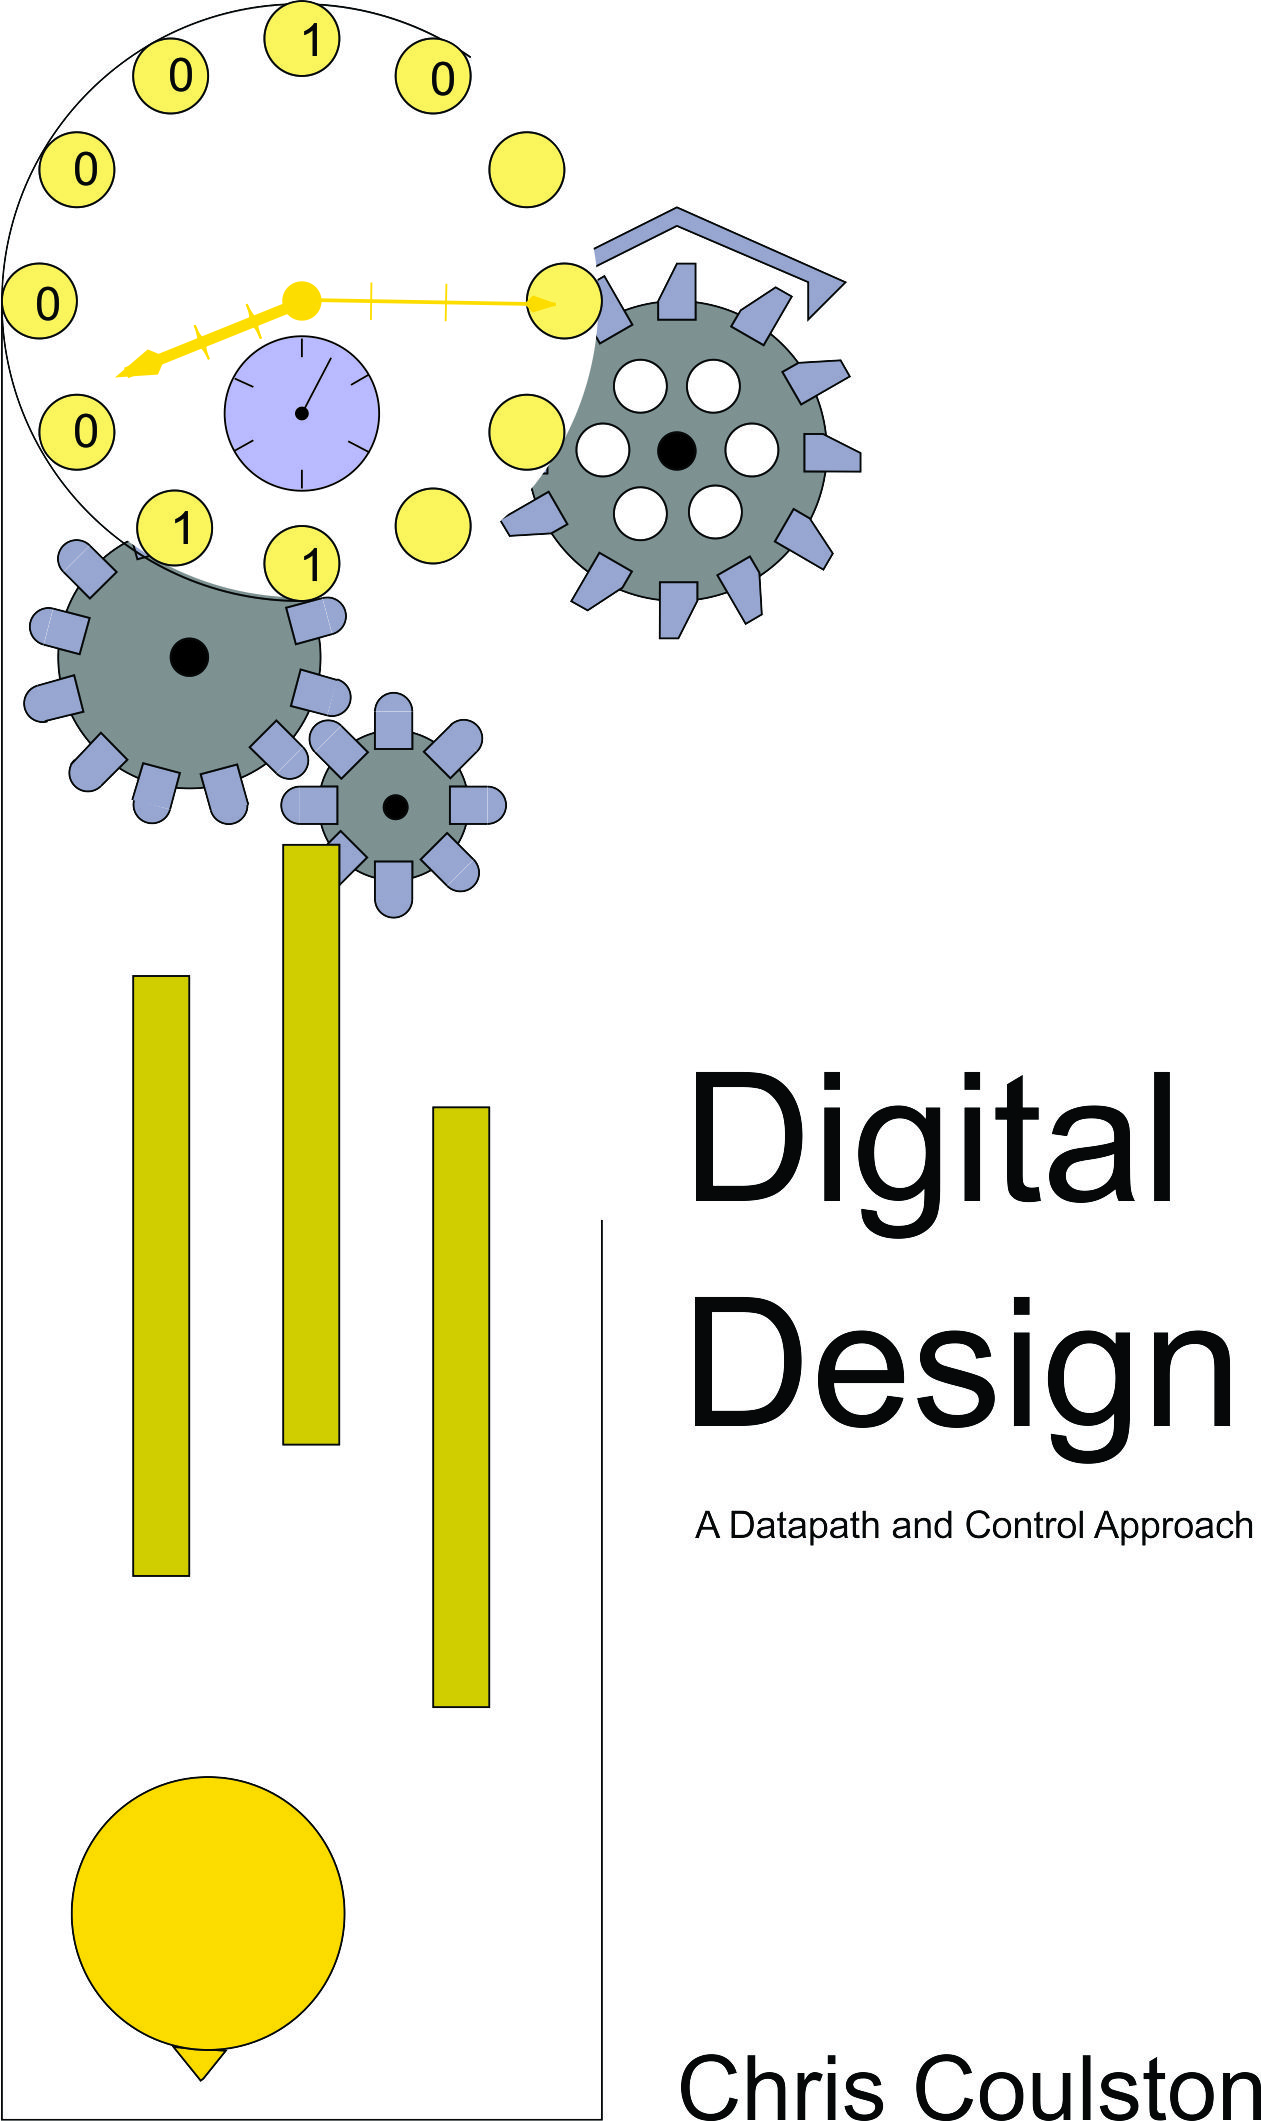
\includegraphics{./Fig/colorCover}
\maketitle

This document was prepared with \LaTeX.
\vspace{2cm}

Digital Design - A Datapath and Control Approach © 2024 by Christopher Coulston is licensed under CC BY-NC-SA 4.0
For more infomation about the Create Commons license see: https://creativecommons.org/licenses/by-nc-sa/4.0/

\begin{figure}[h]
    
\includegraphics[width=1cm]{./Fig/cc-logo.pdf}
    
\includegraphics[width=1cm]{./Fig/cc-by.pdf}
    
\includegraphics[width=1cm]{./Fig/cc-nc.pdf}
    
\includegraphics[width=1cm]{./Fig/cc-sa.pdf}
\end{figure}

\tableofcontents
\listofprocesses
\listofbuildingblocks

%\showanswers
\hideanswers

\mainmatter

\chapter{Numbering Systems}
\label{chapter:NumberingSystems}
\graphicspath{ {./chapter01/Fig} }

The goal of this textbook is to teach students how to design digital systems.
To understand what this means, it is necessary to understand the behavior of
a digital system.  A digital system is a device which receives binary
numbers as input and generates binary numbers as output.  A binary number
is a number composed of bits, or binary digits.  A bit is equal to 
0 or 1.  Generally, bits are represented by voltages, a 0 by a ground 
potential and a 1 by a 3.3v or 5v potential.  However, for most of this 
text, the physical representation of bits will take a back seat to the
the logical representation.  Figure~\ref{fig:chap01sys} shows 
a digital system with three bits of input and two bits of output.

\begin{figure}[ht]
\center{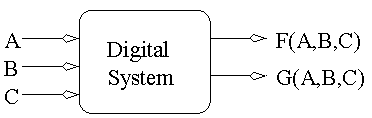
\includegraphics{sys}}
\caption{An abstract digital system with three bits of input
labeled A,B,C and two bits of output, F(A,B,C) and G(A,B,C).}
\label{fig:chap01sys}
\end{figure}

The letters $A,B,C$ in Figure~\ref{fig:chap01sys} represent \textit{ Boolean variables}, 
\index{Boolean variable} variables which are only allowed to assume the values 
0 or 1.  The notation $F(A,B,C)$ means that the output depends on the values 
of $A,B,C$. 

Unfortunately, there is a disconnect between the normal way of describing
quantities using the digits $0 \ldots 9$ and that used by digital systems
using the bits $0,1$.  The study of digital systems starts by describing
the numbering system used to describe decimal numbers and binary numbers.  
These systems are
\textit{ positional numbering systems} \index{numbering system!positional} 
- the position of a digit in a number determines its significance.  The
familiar decimal numbering system is used to illustrate the main concepts
in positional numbering system.

\section{Decimal}
The goal of any numbering system (this includes both
decimal and binary) is to represent quantities using a fixed set of
symbols.  One feature which distinguishes numbering systems is 
the number of symbols used to represent quantities, the numbering 
system's \textit{ base} \index{numbering system!base}.

Decimal is a base-10 numbering system where quantities are expressed using 
10 symbols $\{0,1,2,3,4,5,6,7,8,9\}$.  To explicitly denote a 
number's base, include the base as a subscript after the number.  For example, 
the number of days in a year could be represented as $365_{10}$. 

Each digit in a number represents a quantity which depends on the digit, 
the base, and the position of the digit.  The value of a digit is determined 
by the formula $d * b^i$ where $d$ is the digit, $i$ is the position of the 
digit and $b$ is the base.  The position of the digit immediately to the 
left of the decimal point is 0, every other digit is indexed starting from 
this position.  The value of a multidigit number is the sum of the values of 
the digits, $\sum_{i=0}^N d_i*b^i$, where $N$ is the number of digits in
the number.  Thus $365_{10}$ is interpreted as 
$$3*10^2 + 6*10^1 + 5*10^0 $$

The leftmost digit is called the most significant
digit and the rightmost digit is called the least 
significant digit.  

\section{Binary}
Binary is a base-2 numbering system where quantities are expressed using
two symbols $\{0,1\}$.  When verbally communicating a binary value like $101_2$,
do not say ``one hundred and one base two".  The term \textit{ hundred} is a decimal 
concept and implies the quantity being described is decimal, contradicting
the ``base two".  Instead,  say ``one zero one base two", with the ``base
two" part being optional.   Enough about the nomenclature used to communicate
binary numbers, how to represent values in binary?  Since binary is a 
positional numbering system, then apply the formula $\sum_{i=0}^N d_i*b^i$.

\subsection{Binary to Decimal}
The value of $101_2$ is interpreted as 
$$101_2 = 1*2^2 + 0*2^1 + 1*2^0 = \\
1*4_{10} + 0*2_{10} + 1*1_{10} = \\
4_{10} + 0_{10} + 1_{10} = 5_{10}$$

Application of the positional numbering formula to a binary number
converts it into a decimal number.  As in the decimal case 
there are special names for two of the bits. The leftmost bit is 
called the most significant bit (MSB) and the 
rightmost bit is called the least significant 
bit (LSB).  As a final example, convert $1101_2$ to decimal.

$$1*2^3 + 1*2^2 + 0*2^1 + 1*2^0 = \\
1*8_{10} + 1*4_{10} + 0*2_{10} + 1*1_{10} = \\
8_{10} + 4_{10} + 0_{10} + 1_{10} = 13_{10}$$
\label{page:bin2dec}


\subsection{Decimal to Binary}
In order to provide inputs to a digital system, real world values
represented in decimal need to be converted into binary.
While there are several ways to perform
this conversion, it makes sense to adapt a familiar procedure, 
the binary to decimal conversion.  The key idea is to represent the 
decimal number as the sum of distinct powers-of-two.  To assist in this
procedure, use a power-of-two table.
\\ \\
\begin{tabular}{|c|c|c|c|c|c|c|c|c|c|c|}\hline
$i$   & 0 & 1 &  2 &  3 &  4 &  5 &  6 &  7  &  8  &  9  \\ \hline
$2^i$ & 1 & 2 &  4 &  8 & 16 & 32 & 64 & 128 & 256 &  512\\ \hline 
\end{tabular}
\\ \\
The power-of-two table lists indices, $i$, and its value when it is
raised to the exponent of 2.  This table is used in the following
3-step decimal to binary conversion procedure.

\begin{description}
\item [Step 1] Find the largest power of two less than or equal to the 
number to convert.  
\item [Step 2] Subtract this power of two from the number being converting.
This is the remaining number to convert.
\item [Step 3] If the reminder is not equal to 0, go to step 1; otherwise stop.
\end{description}

The set of values found in Step 1 are the distinct powers-of-two that
when added together equal the number to be converted.  The conversion
is completed by putting the sum into the positional numbering notation.  
The procedure is now applied to convert $13_{10}$ into binary.

\begin{tabular}{ll}
Step & Action \\
1 & The largest power-of-two less than or equal to 13 is 8. \\
2 & The remaining number to convert is 13-8=5. \\
3 & The new remainder is not 0. \\
1 & The largest power-of-two less than or equal to 5 is 4. \\
2 & The remaining number to convert is 5-4=1. \\
3 & The new remainder is not 0. \\
1 & The largest power-of-two less than or equal to 1 is 1. \\
2 & The remaining number to convert is 1-1=0. \\
3 & The new remainder is 0 so the conversion is complete. \\
\end{tabular}

Thus, $13_{10} = 8+4+1$.  This derivation can also be expressed in the
positional numbering notation as follows.

$$13_{10} = 8_{10} + 4_{10} + 1_{10} = 1*2^3 + 1*2^2 + 1*2^0 $$

At this point the ``missing" powers of two are included in the
summation by setting their coefficients to 0.  In the final step, all
the coefficients are stripped off to form the binary number.  Continuing
with the previous example,

$$13_{10} = 1*2^3 + 1*2^2 + 0*2^1 + 1*2^0 = 1101_2$$

Notice that this derivation is the exact reverse of the binary to
decimal conversion shown on page~\pageref{page:bin2dec}.  


\label{page:two-to-N}
What range of values can be described by $N$ bits?  Clearly, the smallest 
number to be represented is 0.  To determine the largest number 
calculate how many different binary numbers can be formed with $N$ bits.
Each bit can be written in two different ways, 0 or 1. Since these choices
are independent events, then the total number of 
possible outcomes is the product of the individual events.  Hence, the 
number of ways to arrange $N$ bits is equal to $2*2* \ldots *2$ ($N$ times) 
which is equal to $2^N$.  Thus, $N$ bits can be arranged in $2^N$ different 
ways. Since 0 is the smallest binary number then the maximum binary number
is $2^N-1$.  The range of an $N$-bit binary number can be represented
as $[0,2^{N}-1]$, where the $[$ and $]$ symbols mean that values 0 and
$2^{N}-1$ are included in the range. 


\section{Hexadecimal}
Hexadecimal is a base-16 numbering system where quantities are expressed using
16 symbols $\{0,1,2,3,4,5,6,7,8,9,A,B,C,D,E,F\}$.  The symbols
$\{A \ldots F \}$ represent quantities just like the symbols $\{0 \ldots 9 \}$.
The symbol $A$ represents the quantity 10, $B$ 11, $C$ 12, $D$ 13, $E$ 14, and
$F$ 15.  So if humans had adopted the hexadecimal numbering system instead of 
decimal you might say to a friend, ``I had $A$ friends over for a party last 
night"  meaning that 10 people showed up. To show how hexadecimal is used 
as a shorthand for binary, consider the conversion of hexadecimal numbers
into binary.

\subsection{Hexadecimal to Binary}
To convert a number from hexadecimal to binary, \textit{ unpack} it.  That is, 
each hexadecimal digit is converted into a 4-bit binary representation.  
This conversion 
is possible because four bits exactly represents every hexadecimal digit
as shown in Table~\ref{table:First16}.

\begin{table}
\begin{center}
\begin{tabular}{|c|c|c|c|}\hline
Decimal & Binary & Hexadecimal \\ \hline
0	& 0000	& 0	 \\ \hline
1	& 0001	& 1	 \\ \hline
2	& 0010	& 2	 \\ \hline
3	& 0011	& 3	 \\ \hline
4	& 0100	& 4	 \\ \hline
5	& 0101	& 5	 \\ \hline
6	& 0110	& 6	 \\ \hline
7	& 0111	& 7	 \\ \hline
8	& 1000	& 8	 \\ \hline
9	& 1001	& 9	 \\ \hline
10	& 1010	& A	 \\ \hline
11	& 1011	& B	 \\ \hline
12	& 1100	& C	 \\ \hline
13	& 1101	& D	 \\ \hline
14	& 1110	& E	 \\ \hline
15	& 1111	& F	 \\ \hline
\end{tabular}
\caption{The first 16 counting numbers represented in 
decimal, binary, and hexadecimal.}
\label{table:First16}
\end{center}
\end{table}

In order to convert $1DAD_{16}$ to binary, replace each hexadecimal
digit with its binary counterpart by consulting Table~\ref{table:First16}.
For example $1DAD_{16} = 0001~1101~1010~1101_{2}$.  The spaces between the
binary numbers are included to make reading the number easier.

\subsection{Binary to Hexadecimal}
The above procedure can be reversed to convert binary numbers into 
hexadecimal.  Group the bits into sets of four, starting at the least
significant bit, then convert each set of four bits into its corresponding
hexadecimal digit in Table~\ref{table:First16}.  
If there are not four digits in the most significant 
grouping, then just add 0s to make a grouping of three -- that is 
pad the number with zeros.  For example, convert  $1110101011_2$ into 
hexadecimal. $1110101011_2 = 0011~1010~1011 = 3AB_{16}$.

To understand why this conversion works, consider the binary 
number $1110101011_2$.  Start by writing down this number using the 
technique from the previous section and then convert it to hexadecimal.
\\ \\
{\tiny
$\begin{array}{l}
1110101011_2= \\
1*2^9+1*2^8+1*2^7+0*2^6+1*2^5+0*2^4+1*2^3+0*2^2+1*2^1+1*2^0 = \\
2^8(0*2^3+0*2^2+1*2^1+1*2^0) + 2^4(1*2^3+0*2^2+1*2^1+0*2^0) + 2^0*(1*2^3+0*2^2+1*2^1+1*2^0) =\\
2^8(0011_2) + 2^4(1010_2) +  2^0(1011_2) =\\
2^{4*2}(0011_2) + 2^{4*1}(1010_2) +  2^{4*0}(1011_2) =\\
16^2(0011_2) + 16^1(1010_2) + 16^0*(1011_2) =\\
16^2(3_{16}) + 16^1(A_{16}) + 16^0*(B_{16}) =\\
3AB_{16}
\end{array}$
} 


\section{Addition of Binary Numbers}
\label{page:addition}
The fact that the addition of binary numbers is similar to the 
addition of decimal numbers should not come as a surprise as both
are positional numbering systems. However, when adding binary numbers
with a digital system, it is possible that the result may exceed the
digital system's capacity because the digital system can only accommodate a 
finite number of bit positions.  The number of bits to be 
simultaneously manipulated by a digital system is refereed to as 
its \textit{ word size} \index{word size}.  A digital system with a
word size of N-bits can represent binary numbers in the range 
$[0, 2^N-1]$.  \textit{ Overflow} \index{overflow} occurs when a 
digital system is forced to represent a value outside the range 
of its word size.

The process of adding binary numbers is exactly the same as adding
decimal numbers: Start in the LSB and work towards the 
MSB.  Each of the bit-positions is called a \textit{ bit-slice} 
\index{bit-slice}.  At each bit-slice, the two bits of the sum are
added together along with the carry-in generated in the previous 
bit-slice.  This addition in a bit-slice will generate one bit of 
sum and possibly one bit of carry to the next bit-slice. The addition 
of bits must be performed in base-2, hence the results may look 
strange.  For example, $1_2 + 1_2 = 10_2$. In this case the sum-bit 
equals 0 and the carry-bit equals 1.  Now, consider a more 
complex problem, adding $3+2$ in binary, assuming a word size of 
four bits.  
\\ \\
\begin{tabular}{r|rrrr}
    &   & 1 &   &    \\
 3  & 0 & 0 & 1 & 1  \\
+2  & 0 & 0 & 1 & 0  \\ \hline
 5  & 0 & 1 & 0 & 1  \\ 
\end{tabular}
\\ \\
Notice, one of the additions produced a carry which is
propagated to the next significant bit position.
The next example demonstrates an addition where the 
result is larger than the word size can accommodate.
\\ \\
\begin{tabular}{r|rrrrr}
    & 1 & 1 & 1 & 1 & 1  \\
13  &   & 1 & 1 & 0 & 1  \\ 
+7  &   & 0 & 1 & 1 & 1  \\ \hline
20  & 1 & 0 & 1 & 0 & 0  \\
\end{tabular}
\\ \\
The decimal result, 20, cannot be represented in four bits, hence
the addition produced overflow.  When adding binary numbers,
overflow occurs whenever there is a carry-out from the most
significant bit-slice.  That is, the result requires more bits 
than are available in the word size.

After being introduced to binary numbering it might be tempting
to look at all collections of bits as being binary numbers.
In truth, a collection of bits has no implicit meaning.  The 
sequence of bits, 0101, could just as easily represent the 
value 5 as it could represent the intensity of red on a display.
A collection of bits gets its meaning from the interpretation
used.  When bits are used to represent integer quantities, 
two main interpretations, binary numbering and 2's complement,
predominate.
 
\section{Negative Numbers}
The binary numbering systems is often called an \textit{ unsigned}
numbering representation.  The term unsigned arises from the 
fact that there is no need to write a sign symbol in front of
a binary number because all binary numbers are positive --
the positive sign is implicit.  A \textit{ signed} numbering representation, 
2's complement, is capable of representing both positive and 
negative numbers.

Like binary numbering, 2's-complement numbers exist within the 
confines of a word size.  One way to determine the 2's-complement 
representation of a decimal number $x$, is to write 
down the binary representation for the quantity $2^N+x$ using 
$N$ bits, where $N$ is the word size.  For example, assuming a 
word size of four bits, determine the 2's-complement representation 
for 6.  To do this, compute $2^N + x = 2^4 + 6 = 16+6=22 = 10110_2$.  
Taking the least significant four bits yields $0110$.  

There are two
points to note.  First, this representation is the same as in 
binary numbering.  Second, the 2's-complement value is written
without a subscript 2, because it is not a binary number.  Now
consider the 2's-complement representation of a negative number.

Assuming a word size of four bits, determine the 2's-complement
representation for -6.  Compute 
$2^N + x = 2^4 - 6 = 16-6 = 10 = 01010_2$.  Taking the least
significant four bits yields $1010$.  

To determine the decimal value of a 2's-complement number,
inspect its MSB.  If the MSB is 0, then the number is
positive, hence can be interpreted as a binary number.
If the MSB is 1, then $2^N+x$ must be solved for $x$.
There is, however an easier way to approach this problem.

Negating a 2's-complement number will mean changing 
the sign of the underlying decimal representation.  The
negation of a 2's-complement number, $x$, can be formed
by flipping all the bits of $x$ and then adding 1.  For
example, take the complement of the 4-bit 2's-complement 
number $x=0110$ which equals 6.  Flipping all 
the bits of $x$ yields $1001$.  Adding 1 to this yields 
$1010$, which was previously shown to equal -6. 

This technique aids in interpreting negative 2's-complement 
numbers as follows.  Given a 2's-complement number that is 
negative, form its
negation, convert that to decimal, then stick a negative
sign in front of the decimal representation.  For example,
determine the decimal representation for the 4-bit 2's-complement 
quantity 1010.  Since the MSB is 1, this
2's-complement number represents a negative quantity.
Flipping the bits, 0101, then adding 1, results in 0110.  
This is the representation for 6, so the original 2's-complement 
number 1010 represent -6.

Figure~\ref{fig:chap012wheel} shows every combination of four bits
and their associated 2's-complement representation.

\begin{figure}[ht]
\center{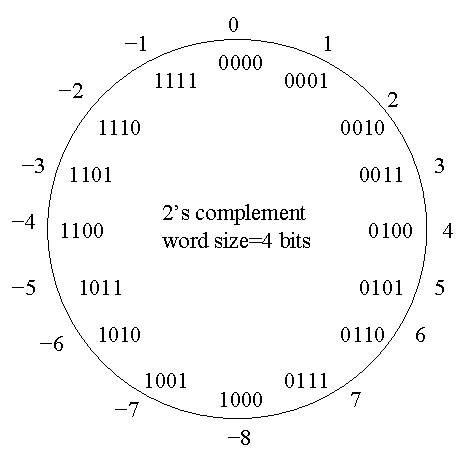
\includegraphics{2wheel}}
\caption{All possible combinations of four bits and their 2's-complement
interpretations.}
\label{fig:chap012wheel}
\end{figure}

Clearly, half of the numbers in Figure~\ref{fig:chap012wheel} have
a leading 0 as their MSB, and are positive; 0 is considered 
a positive number.  The other half of the numbers have their
MSB equal to 1 and are negative.  Since 0 is considered a 
positive number, the largest negative number is 1 larger 
than the largest positive number.  Given a word size of $N$ 
bits the range of 2's-complement numbers is $[-2^{N-1}, 2^{N-1}-1]$.

2's-complement numbers are added in the same way that
binary numbers are added as shown in the 
following three problems.

{\small
\begin{tabular}{ccc}
\begin{tabular}{r|rrrrr}
     &   &   &   &   &     \\
   6 &   & 0 & 1 & 1 & 0   \\
+ -7 &   & 1 & 0 & 0 & 1   \\ \hline
= -1 &   & 1 & 1 & 1 & 1   \\
\end{tabular}
&
\begin{tabular}{r|rrrrr}
     & 1 & 1 & 1 &   &     \\
   3 &   & 0 & 0 & 1 & 1   \\
+ -2 &   & 1 & 1 & 1 & 0   \\ \hline
=  1 &   & 0 & 0 & 0 & 1   \\
\end{tabular}
&
\begin{tabular}{r|rrrrr}
     &   & 1 & 1 &   &     \\
   6 &   & 0 & 1 & 1 & 0   \\
+  6 &   & 0 & 1 & 1 & 0   \\ \hline
= 12 &   & 1 & 1 & 0 & 0   \\
\end{tabular} \\
\end{tabular}
}

The first example, 
$6 + -7$, shows  the addition process working correctly when
the operands have different signs.  The other two problems 
illustrate the need for a new definition of overflow for 2's-complement 
numbers.  The general rule for overflow in 2's complement 
is, \label{page:Ovf} if the carry-in and carry-out 
into and out from the MSB are not equal, then overflow has 
occurred.  The carry-out from the MSB is always thrown away.
For example, the carry-in and carry-out of the MSB in second
problem are both 1, hence the result is valid.  In the third
problem, the carry in to the MSB is 1 and the carry-out from the
MSB is 0, hence overflow has occurred.  This result should not be a 
surprise because the expected result, 12, cannot be represented
as a 4-bit 2's-complement number.

Taking the complement of a 2's-complement number allows subtraction
problems to be converted into addition problems.  \label{page:2sub}
For example, the subtraction problem $3 - 2$ can be rewritten as 
$3 + (-2)$.

\begin{tabular}{ccc}
\begin{tabular}{r ccccc}
   3 &   & 0 & 0 & 1 & 1   \\
- +2 &   & 0 & 0 & 1 & 0   \\ \hline
\end{tabular} 
& Becomes &
\begin{tabular}{r ccccc}
     & 1 & 1 & 1 &   &     \\
   3 &   & 0 & 0 & 1 & 1   \\
+ -2 &   & 1 & 1 & 1 & 0   \\ \hline
=  1 &   & 0 & 0 & 0 & 1   \\
\end{tabular} \\

\end{tabular}
\\ \\
Situations will arise which require increasing the number of bits 
required to represent a number while retaining the value of the
number.  For example, imagine having a 
4-bit binary number that must be stored in a device that holds 
eight bits.  How can this be done while preserving
the magnitude of the number?  For binary numbers, the answer is
easy, add 4 leading zeros, an operation called \textit{ padding with 0s}.  

For 2's-complement numbers this 
solution will not work.  For example, consider the
4-bit 2's-complement representation for -1 (1111) that needs to
be store in a 8-bit device.  Adding 4 leading 0s 
will change the value of the number to 00001111, the value 
15.  The solution, in this case, is to pad with 1s, yielding
11111111, which represents -1 in 8-bit 2's complement.  As 
with the binary numbering example,
positive 2's-complement numbers can be padded with 0s and
still retain their value.  The general rule for padding
in 2's complement is called \textit{ sign extension}; 
\index{sign extension} \label{page:2sPad} and involves copying 
the MSB to fill in the needed space.  
Table~\ref{table:SignExt} shows five examples of sign extension
on 2-bit 2's-complement numbers.

\begin{table}
\begin{center}
\begin{tabular}{l|l}
4-bit 2's complement & 8-bit 2's complement \\ \hline
1110=-2			& 11111110=-2 \\ \hline
1010=-6			& 11111110=-6 \\ \hline
1000=-8			& 11111000=-8 \\ \hline
0011=3			& 00000011=3 \\ \hline
0111=7			& 00000111=7 \\ 
\end{tabular}
\caption{Five examples showing how to sign-extend a 4-bit
2's-complement number.}
\label{table:SignExt}
\end{center}
\end{table}

\section{Other codes}

\subsection{Octal}

\subsection{Grey Code}

\subsection{Ones Hot}

\subsection{ASCII}

\subsection{BCD}

\subsection{Fixed Point}

\subsection{Floating Point}


\section{Exercises}
\label{section:chap01Exercises}

\begin{enumerate}
\item \textbf{ (1 pt. each)} Syllabus:
	\begin{enumerate}
	\item What is the late penalty for homework?
	
	\begin{onlysolution}
	\itshape
	There is a 33\% deduction per day.
	\end{onlysolution}

	\item True or False: Calculators can be used during exams.
	
	\begin{onlysolution}
	\itshape
	You cannot use calculators at my exams.
	\end{onlysolution}
	
	
	\item True of False: University ID is required during exams.
	
		
	\begin{onlysolution}
	\itshape
	I check ID at the exams.  After I learn 
		your names its not such a big
		deal, but bring it to be safe.
	\end{onlysolution}
	
	\item What is my thesis regarding grades?
	\item Bob L. Student has the following grades.  Determine his final
	overall course percentage and grade.

		\begin{tabular}{l|l}
		Component & Percentage \\ \hline \hline
		Homework & $60\%$ \\ \hline
		Exam 1	 & $90\%$ \\ \hline
		Exam 2	 & $80\%$ \\ \hline
		Final	 & $70\%$ \\ 
		\end{tabular}


	\begin{onlysolution}
	\itshape
                \begin{tabular}{l|l|l}
                Component & Percentage & Weight \\ \hline \hline
                Homework & $60\%$    & 60*0.35 = 21\\ \hline
                Exam 1   & $90\%$    & 90*0.20 = 18\\ \hline
                Exam 2   & $80\%$    & 80*0.20 = 16\\ \hline
                Final    & $70\%$    & 70*0.25 = 17.5 \\ \hline
                Total    & $72.5\%$ & C \\
                \end{tabular}
	\end{onlysolution}

	\item How should you prepare for the 43$^{rd}$ lecture?

	\begin{onlysolution}
	\itshape
	 Look over homework problem 8.10, page 165
	 \end{onlysolution}
	 
	\end{enumerate}

\item \textbf{ (1 pt. each)} Convert the following numbers to decimal. 
Show work, or receive 1/2 credit.
	\begin{enumerate}
	\item $100_2$
	\begin{onlysolution}	\itshape $100_2 = 2^2 = 4_{10}$\end{onlysolution}
	
	\item $1000_2$
	\begin{onlysolution}	\itshape $1000_2 = 2^3 = 8_{10}$\end{onlysolution}
	
	\item $10000_2$
	\begin{onlysolution}	\itshape $10000_2 = 2^4 = 16_{10}$\end{onlysolution}
	
	\item $100000_2$
	\begin{onlysolution}	\itshape $100000_2 = 2^5 = 32_{10}$\end{onlysolution}
	
	\item $111111_2$
	\begin{onlysolution}	\itshape $111111_2 = 2^5+2^4+2^3+2^2+2^1+2^0=63_{10}$\end{onlysolution}
	
	\item $1000100101000101_2$
	\begin{onlysolution}	\itshape $1000100101000101_2=2^{15}+2^{11}+2^8+2^6+2^5+2^0=35141_{10}$\end{onlysolution}
	
	\item $3EA_{16}$
	\begin{onlysolution}	\itshape$3EA_{16}=0011 1110 1010 = 2^9+2^8+2^7+2^6+2^5+2^3+2^1=1002_{10}$\end{onlysolution}
	
     \end{enumerate}


\item \textbf{ (1 pt. each)} Convert the following number to binary. Show 
work, or receive 1/2 credit.
	\begin{enumerate}
	\item $44_{16}$
	\begin{onlysolution}	\itshape $44_{16} =0100 0100_2$\end{onlysolution}
	
	\item $44_{10}$
	\begin{onlysolution}	\itshape $44_{10} = 32+8 = 2^5+2^3=101100_2$\end{onlysolution}
	
	\item $1023_{10}$
	\begin{onlysolution}	\itshape$1023_{10} = 512+256+128+64+32+16+8+4+2+1=
        2^9+2^8+2^7+2^6+2^5+2^4+2^3+2^2+2^1+2^0=1111111111_2$\end{onlysolution}
        
	\end{enumerate}


\item \textbf{ (1 pt. each)} Convert the following number to hex. Show work, or receive 1/2 credit.
	\begin{enumerate}
	
	\item $101011101_2$
	\begin{onlysolution}	\itshape$1 0101 1101_2 = 15D_{16}$ \end{onlysolution}
	
	\item $77_{10}$
	\begin{onlysolution}	\itshape $77_{10} = 64+8+4+1=2^6+2^3+2^2+2^0=100 1101_2=4D_{16}$ \end{onlysolution}
	
	\end{enumerate}


\item \textbf{ (2 pts. each)} Toughies:
	\begin{enumerate}
	\item Convert $123_5$ to base-12
	\begin{onlysolution} 	\itshape
		$123_5 = 1*5^2 + 2*5^1 + 3*5^0 = 25+10+3=38_{10}=
        3*12^1 + 2*12^0 = 32_{12}$ \end{onlysolution}
        
	\item Convert $789_{12}$ to base-5
	\begin{onlysolution}
	\itshape	$789_{12} = 7*12^2+8*12^1+9*12^0=1008+96+9=1113_{10}= \\
        1*5^4+3*5^3 + 4*5^2 + 2*5^1 + 3*5^0 = 13423_5$ \end{onlysolution}
        
	\item What is the largest base-10 quantity that can be represented
	using 5 digits in base 12?

	\begin{onlysolution}
	\itshape $BBBBB_{12} = 11*12^4+11*12^3+11*12^2+11*12^1+11*12^0=248831_{10}$ \end{onlysolution}
	
	\end{enumerate}


\item \textbf{ (1 pt. each)} Perform the following additions, assume a word 
size of four bits. Determine if overflow occurs.
	\begin{enumerate}
	
	\item $0110_2 + 0101_2$
	\begin{onlysolution}	\itshape0110 + 0101 = 1011\end{onlysolution}
	
	\item $0010_2 + 0110_2$
	\begin{onlysolution}	\itshape0010 + 0110 = 1000\end{onlysolution}
	
	\item $0111_2 + 0011_2$
	\begin{onlysolution}	\itshape0111 + 0011 = 1010\end{onlysolution}
	
	\item $0010_2 + 0101_2$
	\begin{onlysolution}	\itshape0010 + 0101 = 0111\end{onlysolution}
	
	\item $0010_2 + 1010_2$
	\begin{onlysolution}	\itshape0010 + 1010 = 1100\end{onlysolution}
	
	\item $0101_2 + 1011_2$
	\begin{onlysolution}	\itshape0101 + 1011 = 10000 overflow\end{onlysolution}
	
	\item $0011_2 + 1001_2$
	\begin{onlysolution}	\itshape0011 + 1001 = 1100\end{onlysolution}
	
	\end{enumerate}
\end{enumerate}


\chapter{Representations of Logical Functions}
A digital system starts its life deep inside an engineer's mind.  
In the beginning it is an abstract device; its very far removed 
from reality.  In order to realize the digital system, the engineer
undertakes the design process; a series of refinements to bring
the digital system closer and closer to a real working system.  This 
iterative approach is necessary in complex designs because going straight
to a final implementation is overwhelming, error-prone, difficult
to modify, and difficult to debug and test.  The goal in breaking the 
design process into steps is to allow the proper specification of the
digital system using a ``language" which is easy to understand and modify,
and then to show how to implement this specification using real circuit 
elements. 

Four refinements in the design of digital systems are 
considered.  Each of these refinements define the input, output, and 
behavior of the digital system.  

\begin{description}
\item [Word Statement] - A written description of the expected 
	input, output, and behavior of the digital system.
\item [Truth Table] -  A listing of every possible input to the
	digital system and the corresponding output.  
\item [Symbolic] - A symbolic (math-like) description of the 
	output(s) as a function of the input variable(s).
\item [Circuit Diagram] - A pictorial representation of the 
	physical interconnections of the circuit elements.
\end{description}

When designing a digital system each of these representations should
describe the same system, just in different ways.  The most abstract 
representation of a digital system is the word statement.  Word 
statements are notoriously ambiguous and have no standardized structure.  
However, these shortcomings are the strengths of this representation. The great
expressibility of language allows very complex processes to be captured 
in brief statements.  Hence, ideas can be quickly refined 
without having to expend much engineering effort.  Also, because 
word statements have no prescribed form, there is a great deal 
of flexibility in structuring a word statements.  Because of its
potential ambiguity and unclear boundaries, the word statement's step 
in the design process diagram shown in Figure~\ref{fig:Design} is 
drawn inside a puffy cloud.

\begin{figure}[ht]
\center{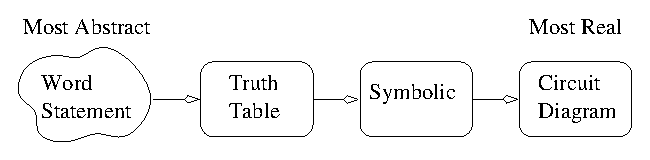
\includegraphics{./Fig2/Design}}
\caption{The steps in the design of a digital system.}
\label{fig:Design}
\end{figure}

Each of the four design stages shown in Figure~\ref{fig:Design} 
is a description of a digital system.  The arrows in 
Figure~\ref{fig:Design} are 
transformations described in this chapter.  

After the word statement, all subsequent stages of the design process
are unambiguous, they have one clearly understood interpretation.  The first
refinement of a word statement is a truth table.  The truth table strikingly 
illustrates the difference between digital and analog circuits.  When
working with analog phenomena, like the AC voltage from a wall outlet,
it is impossible to list all possible values of the voltage, because 
an infinite number of potential values exists.  However, when working
with digital phenomena, each signal can have only one of two possible values,
making it quite easy to enumerate them all.  When working with a
digital system with three bits of inputs, like that shown in 
Figure~\ref{fig:sys}, there are only eight
different combinations of the inputs.  For each of these input 
combinations, a truth table specifies what the output should be.  

The symbolic form is a set of equations written in Boolean Algebra.
These equations look similar to those encountered
in an algebra class. However, instead of operations like addition 
and multiplication, Boolean Algebra uses the operations AND, OR, and 
NOT.  These operations have hardware counterparts - real physical 
circuits which ``compute" their values.  A circuit diagram shows how
these hardware components are interconnected to realize the 
digital system.  As real devices, these circuits represent the bit 
values, 0 and 1 as voltages.  Typically, logic 1 is represented by 
a high voltage level (5v) and logic 0 is represented by a low 
voltage level (0v). 

This text takes a bottom-up approach in designing digital systems.  
The design process starts with the most fundamental digital hardware 
components and shows how they are interconnected to form basic building 
blocks.  These building blocks are then arranged into datapath and 
control circuit.  Thus, all the digital circuits studies in this text
will be built from a small pallet of fundamental digital hardware 
components, called the elementary logical functions.

\section{Elementary Logical Functions}

Elementary logical functions get their name because they are 
the fundamental (elementary) building blocks of digital design, they 
use the logical operators like AND, OR, and NOT (logical), and 
they describe a transformation (function) from input to output.  For each 
elementary logical function, its word statement, truth table, symbolic and 
circuit diagram are presented.


\label{page:elf1}
\begin{tabular}{ll}

{\huge AND} & 
\begin{tabular}{l|l}
Word Statement &  
\begin{tabular}{l}
AND is a logical function with two inputs and   \\
one output.  The output equals 1 only when all the \\
inputs are equal to 1, otherwise the output   \\
equals 0. 
\end{tabular} \\ \hline
Symbolic  & A*B \\ \hline
Truth Table &
	\begin{tabular}{c|c||c}
	A & B & A*B \\ \hline \hline
	0 & 0 & 0   \\ \hline
	0 & 1 & 0   \\ \hline
	1 & 0 & 0   \\ \hline
	1 & 1 & 1   \\ 
	\end{tabular} \\ \hline
Circuit Diagram & 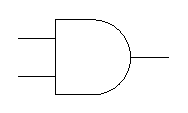
\includegraphics{./Fig2/and} \\
%% \end{tabular} \\ \hline \hline
\end{tabular} \\ 
\end{tabular}

\begin{tabular}{ll}
{\huge OR} &
\begin{tabular}{l|l}
Word Statement &
\begin{tabular}{l}
OR is a logical function with two inputs and one  \\
output.  The output equals 1 when any input  \\
is equal to 1, otherwise the output equals 0. \\
\end{tabular} \\ \hline
Symbolic &  A+B \\ \hline
Truth Table &
	\begin{tabular}{c|c||c}
	A & B & A+B \\ \hline \hline
	0 & 0 & 0   \\ \hline
	0 & 1 & 1   \\ \hline
	1 & 0 & 1   \\ \hline
	1 & 1 & 1   \\ 
	\end{tabular} \\ \hline
Circuit Diagram & 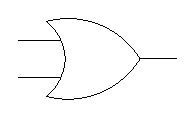
\includegraphics{./Fig2/or} \\
\end{tabular} \\ \hline \hline

{\huge NOT} & 
\begin{tabular}{l|l}
Word Statement &
\begin{tabular}{l}
NOT is a logical function with one input and one  \\
output.  The output is not equal to the input. \\
\end{tabular} \\ \hline
Symbolic & A' \\ \hline
Truth Table &
	\begin{tabular}{c||c}
	A & A' \\ \hline \hline
	0 & 1   \\ \hline
	1 & 0   \\ 
	\end{tabular} \\ \hline
Circuit Diagram & 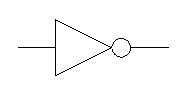
\includegraphics{./Fig2/not} \\
\end{tabular} \\ \hline \hline

{\huge NAND} & 
\begin{tabular}{l|l}
Word Statement &
\begin{tabular}{l}
NAND is a logical function with two inputs and \\
one output.  The output equals 1 when any input \\
is equal to 0, otherwise the output equals 0. \\
\end{tabular} \\ \hline
Symbolic &  (A*B)' \\ \hline
Truth Table & 
	\begin{tabular}{c|c||c}
	A & B & (A*B)' \\ \hline \hline
	0 & 0 & 1   \\ \hline
	0 & 1 & 1   \\ \hline
	1 & 0 & 1   \\ \hline
	1 & 1 & 0   \\
	\end{tabular} \\ \hline
Circuit Diagram & 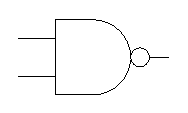
\includegraphics{./Fig2/nand} \\
\end{tabular} \\ \hline \hline
\end{tabular}

\begin{tabular}{ll}
{\huge NOR} & 
\begin{tabular}{l|l}
Word Statement & 
\begin{tabular}{l}
NOR is a logical function with two inputs and  \\
one output.  The output equals 0 when any input  \\
is equal to 1, otherwise the output equals 0. \\
\end{tabular} \\ \hline
Symbolic & (A+B)' \\ \hline
Truth Table &
	\begin{tabular}{c|c||c}
	A & B & (A+B)' \\ \hline \hline
	0 & 0 & 1   \\ \hline
	0 & 1 & 0   \\ \hline
	1 & 0 & 0   \\ \hline
	1 & 1 & 0   \\
	\end{tabular} \\ \hline
Circuit Diagram & 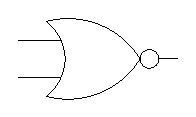
\includegraphics{./Fig2/nor} \\
\end{tabular} \\ \hline \hline

{\huge XOR} & 
\begin{tabular}{l|l}
Word Statement &
\begin{tabular}{l}
XOR is a logical function with two inputs and  \\
one output.  The output equals 1 when the inputs  \\
are different, otherwise the output is equal  \\
to 0.
\end{tabular} \\ \hline
Symbolic & $A \oplus B$ \\ \hline
Truth Table &
	\begin{tabular}{c|c|c}
	A & B & A $\oplus$ B \\ \hline \hline
	0 & 0 & 0   \\ \hline
	0 & 1 & 1   \\ \hline
	1 & 0 & 1   \\ \hline
	1 & 1 & 0   \\ 
	\end{tabular} \\ \hline
Circuit Diagram & 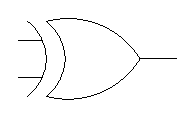
\includegraphics{./Fig2/xor} \\
\end{tabular} \\ \hline \hline
%% \caption{The elementary logical functions.}
%% \label{table:elf}
\end{tabular}
\label{page:elf2}

The physical elements for the elementary logical functions are
typically called {\it gates}.   Thus, the physical circuit for 
the AND logical function is called an AND gate.

The AND/OR functions can be enlarged to handle more than
two inputs because their word statements use words ALL/ANY
respectively.  Thus a 4-input AND gate will output 1
only when all four inputs equal 1.  The circuit diagram for 
this AND gate would look just like a 2-input AND gate with
two additional inputs.

\section{Conversion Between Representations}
Figure~\ref{fig:forms} shows the four representations of a digital system
along with the different transformations covered in this section.  
The arrows are numbered by the subsection in which the transformation is
covered.  The design process shown in Figure~\ref{fig:Design} is captured
in Steps 7, 6, and 3.  The other transformations introduced in this 
section enable designs to be optimized as well as to explore 
the relationships between the representations.

\begin{figure}[ht]
\center{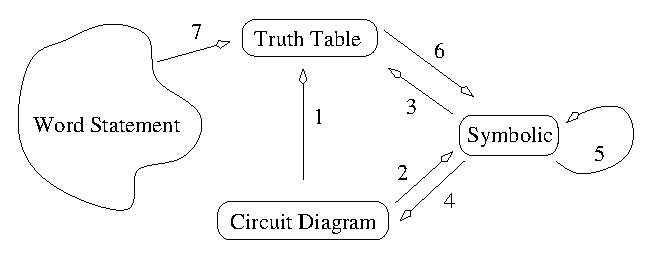
\includegraphics{./Fig2/forms}}
\caption{The four representations of a logical function.  The
numbered arrows are the transformations examined in this chapter.}
\label{fig:forms}
\end{figure}

\subsection{Circuit Diagram to Truth Table}

The first transformation is the circuit diagram to truth table.  
Where the circuit diagram came from is unimportant for now.
Figure~\ref{fig:CD-TT} is a circuit diagram with three bits of 
input labeled $A,B,C$ and one bit of output $F(A,B,C)$ that will
be transformed into a truth table.

\begin{figure}[ht]
\center{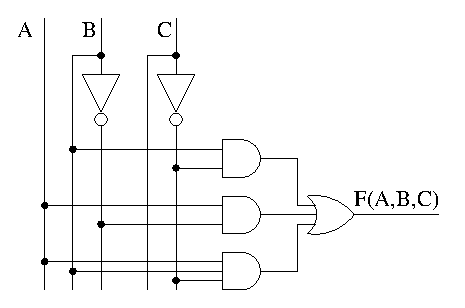
\includegraphics{./Fig2/cd-tt}}
\caption{A simple 3-input, 1-output circuit.}
\label{fig:CD-TT}
\end{figure}

Before starting with the transformation there are some important
observations to make about Figure~\ref{fig:CD-TT}.  The gates in a circuit 
may have different numbers of inputs.  For example, this circuit contains 
two AND gates with two bits of input and an AND gate with three bits of
input.  Next, the lines drawn in the figure represent physical wire.
When a voltage is applied to one end of the wire by an external source
or by one of the gates, it is assumed to propagate instantaneously to 
all points on the wire.  The black dots on intersecting wires means 
that the two wires are connected.  For example, the vertical wire
labeled ``$A$" is connected to the second and third AND gates. 
 Wires that cross one another and do not have a dot are assumed not
to be connected.  For example, the $C$ signal does not go into the
second AND gates.  The output from a gate is always connected to the
input of another gate.  Outputs are never connected directly together, because 
they could create a short-circuit destroying the participating gates.  Inputs 
are always tied to some signal source. Otherwise their values
would float between logic 0 and logic 1, and cause unpredictable 
behavior in the circuit.  Since
the three external inputs in Figure~\ref{fig:CD-TT} do not have sources shown,
they must be provided by some external user.  The output 
from a gate can provide input to multiple, different inputs.  For example, 
the output of the NOT gate
associated with the $C$ input feeds the first and third AND gates. 

The first step in transforming a circuit diagram into a truth table is
to identify the inputs and outputs of the circuit.
Any wire which is not being driven by some source is an input and 
any output which is not driving a source is an output.  In the case of 
Figure~\ref{fig:CD-TT}, $A,B,C$ are inputs and $F(A,B,C)$ is an output.

The second step in the transformation is to build the shell of the truth 
table to hold the solution.  
Remember that, ``A truth table is a listing of every possible  input to the 
digital system and the corresponding output."  For example $A=1$, $B=0$ and 
$C=1$ is a possible input to the circuit.  All the 
potential inputs to the circuit could be listed in a {\it ad-hoc} 
manner, but a much more organized approach is shown below.

\label{page:TTshell}
$$\begin{array}{c|c|c||c}
A & B & C & F(A,B,C) \\ \hline \hline
0 & 0 & 0 &   \\ \hline
0 & 0 & 1 &   \\ \hline
0 & 1 & 0 &   \\ \hline
0 & 1 & 1 &   \\ \hline
1 & 0 & 0 &   \\ \hline
1 & 0 & 1 &   \\ \hline
1 & 1 & 0 &   \\ \hline
1 & 1 & 1 &   \\
\end{array}$$

Two good reasons drive this choice of row ordering.
First, the columns of the truth table have a strong pattern.
The bits of the $C$-variable column repeat from top to bottom, $0 1 0 1 \ldots$.
The bits of the $B$-variable column repeat from top to bottom, two 0s followed by two 1s.
The bits of the $A$-variable column repeat from top to bottom, four 0s followed by four 1s.
Using this pattern makes filling a truth table easier.  Second,
when the $A,B,C$ variables in each row are interpreted as a 
3-bit binary number, they form consecutive integers.  This approach
makes finding a particular input/output much easier.

The third step in the transformation of a circuit diagram into a 
truth table is to determine the values in the $F(A,B,C)$ column.  
In order to do this each input is applied, one at a time, to 
the circuit and determine the output of the circuit.  This step is also
referred to as evaluating the output of the circuit.  

Imagine that 
the bits are flowing down hill from the inputs to the outputs.  A 
gate computes its output only when the values of all its inputs
are known.  The output of a gate is determined from the truth tables
given on pages \pageref{page:elf1} through \pageref{page:elf2}.  For example,
in Figure~\ref{fig:cd-tt2}A, the input $A=B=C=0$ is applied
to the input.  The third AND gate cannot compute its output until
it receives the output from the NOT gate associated with the $C$ 
input.  The outputs from each gate are shown on the signals in
Figure~\ref{fig:cd-tt2}B.  Due to size constraints, the AND gate 
inputs are written inside the gate.  

\begin{figure}[ht]
\center{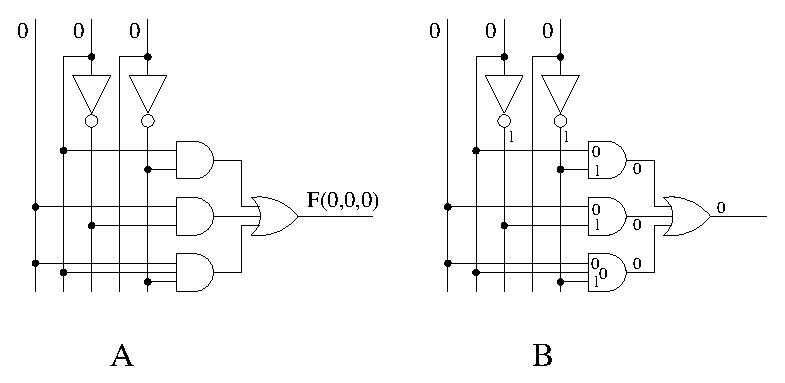
\includegraphics{./Fig2/cd-tt2}}
\caption{A) The circuit diagram from Figure~\ref{fig:CD-TT} with
input $A=B=C=0$.  B) The effect of this input shown on the wires.}
\label{fig:cd-tt2}
\end{figure}

Figures \ref{fig:CD-TT} and \ref{fig:cd-tt2} 
illustrate a subtle notational convention. 
Why is the output of the circuit shown in Figure~\ref{fig:CD-TT} 
labeled $F(A,B,C)$ and in Figure~\ref{fig:cd-tt2}A this same output is
labeled  $F(0,0,0)$?  It is because the variables $A,B,C$ in $F(A,B,C)$ 
are placeholders for the actual values of the variables.  Since these
variables are given the values $A,B,C = 0,0,0$ in Figure~\ref{fig:cd-tt2}A, 
this notational change is acknowledged by labeling the output $F(0,0,0)$.

Since Figure~\ref{fig:cd-tt2}B shows that $F(0,0,0) = 0$, then
a 0 is placed in the top row of the truth table for this 
function.  The remaining seven rows of the truth table are computed 
using this same method.  The resulting truth table is shown below.

$$\begin{array}{c|c|c||c}
A & B & C & F(A,B,C) \\ \hline \hline
0 & 0 & 0 & 0  \\ \hline
0 & 0 & 1 & 0  \\ \hline
0 & 1 & 0 & 1  \\ \hline
0 & 1 & 1 & 0  \\ \hline
1 & 0 & 0 & 1  \\ \hline
1 & 0 & 1 & 1  \\ \hline
1 & 1 & 0 & 1  \\ \hline
1 & 1 & 1 & 0  \\
\end{array}$$

While this transformation provides an excellent introduction to a variety
of important concepts, it is not a practical way to derive the truth table 
entries.  First, it is tedious because the same process must be performed 
eight times.  Second, it is prone to errors because the bits on the figure
must be overwritten seven times, once for every row of the table. 
It turns out that determining the symbolic
form for this circuit's output and then determining the truth table is a
much less tedious and less error-prone method to determine the truth table
from a circuit diagram.

\subsection{Circuit Diagram to Symbolic}
The transformation of a circuit diagram into a symbolic expression 
is very similar to evaluating the output of the circuit, except symbols
instead of bits flow through the circuit.  The symbolic output of 
a gate is written out only when symbolic inputs are present on all of the 
gate's input.  The output of a gate is determined from the symbolic forms
given on pages \pageref{page:elf1} and \pageref{page:elf2}.  For example, in 
order to determine the output of the AND gates in Figure~\ref{fig:basic}A, the
symbolic outputs of the NOT gates must first be determined.  These are
$A', B', C'$ as shown in Figure~\ref{fig:basic}B.

\begin{figure}[ht]
%% scalebox{0.5}{stuff}
\center{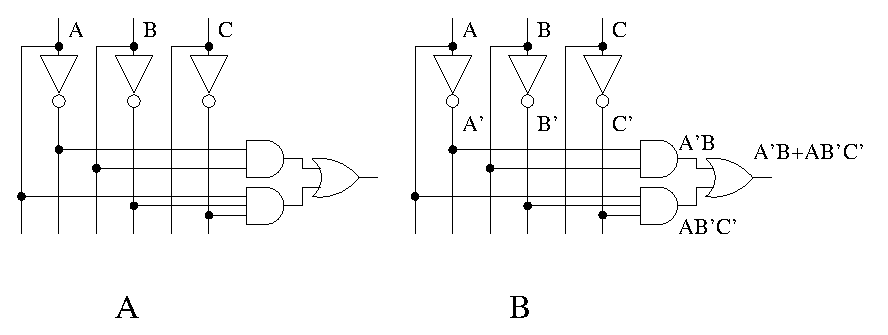
\includegraphics{./Fig2/basic}}
\caption{A) A circuit diagram.  B) The input variables propagated through
to the output.}
\label{fig:basic}
\end{figure}

Since the inputs to the top AND gate are $A'$ and $B$, the output of the AND
gate is labeled $A'B$.  The output was not labeled ``A'*B" because the
``*" is often dropped from the symbolic expressions involving AND 
in order to save space.  This is similar to the convention 
of dropping the ``*" symbol when it is used
as the multiplication operator in regular algebra.  When two Boolean 
variables appear next to one another it is assumed that they are ANDed together.
After labeling the output of the other AND gate, the output of the OR gate 
is labeled $A'B + AB'C'$ as shown in Figure~\ref{fig:basic}B.

It was earlier suggested that in order to determine the truth table for a
circuit diagram, it is easier to first determine the symbolic form for
the circuit diagram, and then determine the truth table from this symbolic 
form.  Determining the symbolic form of a circuit's output is eight times
easier than determining all eight rows of the truth table.
The next subsection will show how to transform a symbolic 
form into a truth table.

\subsection{Symbolic to Truth Table}

Like the transformation of a circuit diagram to a truth table, the
first step in this transformation is to identify the inputs and outputs 
of the circuit.  Normally, the variable on the left-hand side
of the equal sign in an equation is the output and any variables 
which appear on the 
right-hand side are inputs.  For example, in the equation 
$F(A,B,C) = A'B + AB'C'$, $F$ is the output and $A,B,C$ are the inputs.

The second step is to write down the shell of the truth table using the
ordering given on page~\pageref{page:TTshell}.  The basic structure of the
truth table is the same no matter how many variables the symbolic 
expression has.  
For example, if a symbolic expression has four input variables $A,B,C,D$,
then start by listing the variables across the top of the truth table.  
Then write the bit values for the $D$ variable by alternating 0
and 1 on every row, from top to bottom. The $C$ variable would alternate 
every other row, from top to bottom.  The $B$ variable every
fourth row, and the $A$ variable every eighth row.  The resulting 
truth table has 16 rows.  This should not come as a surprise since,
from page~\pageref{page:two-to-N}, there are 
$2^4=16$ different combinations of four input bits.

The third step in the transformation is to evaluate the symbolic 
expression for each combination of inputs.  Evaluation is the process
of substituting each variable's value into the equation and applying 
the operators to the values.  For example, evaluate $F(A,B) = (A+B)'$
for $(A,B) = (0,1)$.  Substituting in the values for the variables
yields $F(0,1) = (0+1)'$.  Applying the OR operation to 0 and 1 gives the 
result 1.  Applying the NOT operator to the result of the OR operator yields 0.
Thus, $F(A,B)$ evaluated at $(A,B)=(0,1)$ equals 0.  In other words,
$F(0,1)=0$.  The evaluation of more complex expressions requires 
a firm grasp on the rules of operator precedence in Boolean Algebra.

The symbolic expressions are written in 
{\it Boolean Algebra}, \index{Boolean Algebra} an algebra where variables
represent the values 0 and 1 and which are joined together using operators 
like AND, OR and NOT.  The symbolic expressions written in a 
high school algebra class have variables which represent real numbers and
are joined together using operators like addition and multiplication.  In 
both algebras, operator precedence must be understood in order to evaluate
complex expressions.  Operator precedence specifies the order in which the
operations of an expression are evaluated.  Operations with higher precedence
are performed before operations with lower precedence.  The rules of operator 
precedence are listed for both algebras in the following table.

\begin{tabular}[ht]{l|l|l}
			& Regular Algebra			& Boolean Algebra \\ \hline \hline
High precedence	& Parenthesis			& Parenthesis	\\ \hline
			& Exponents				& Not			\\ \hline
			& Multiplication/Division	& And			\\ \hline
Low precedence	& Addition/Subtraction 		& Or 			\\
\end{tabular}
\\ \\
Operator precedence is examined by considering the problem of
deriving the truth table for the $F(A,B,C) = A'B + AB'C'$.  This expression
has three input variables and one output variable.  An empty shell of the 
truth table is exactly the same as the one shown on 
page~\pageref{page:TTshell}.  

Next, the expression is evaluated for every possible input.  In 
other words, determine $F(0,0,0) \ldots F(1,1,1)$.  Start with 
the first row of the truth table and determine $F(0,0,0)$ by
substituting $0,0,0$ for every occurrence of $A,B,C$ in the symbolic 
expression.  This yields $0'*0+0*0'*0'$.  In order to evaluate this expression, 
perform the highest precedence operator first.  In this case, evaluate 
the three NOTs yielding, $1*0+0*1*1$.  The next highest 
precedence operator is AND, evaluating the two ANDs in the expression 
yields, $0+0$.   Evaluating the remaining OR yields 0.  Hence, $F(0,0,0)=0$.

Continuing this procedure of evaluating the function for the remaining seven
inputs, would result in the same problems encountered when converting  a
circuit diagram into a truth table namely, that the
process is tedious and error prone.  In order to make good on the 
promise to produce an efficient transformation of a circuit diagram 
to a truth table, a better method is needed to complete the truth table
from the symbolic form.

Two conditions make evaluating a symbolic expression
difficult: its size and the evaluation process itself.  Each difficulty
will be addressed in turn.  Instead of treating the symbolic expression 
as a single monolithic entity, break the expression into smaller
subexpressions, evaluate each subexpression for all the inputs, and 
then put the values of the subexpressions back together.  Three criteria govern
the decomposition of an expression into subexpressions. First, break the 
the expression into as few pieces as possible.  Second, break the expression 
into subexpressions which are easy to put back together.  Third, break the
expression into subexpressions which are easy to evaluate.  

For example, look at the expression $A'B + AB'C'$.  This expression splits nicely
into two subexpressions $A'B$ and  $AB'C'$.  This division meets the three
criteria, only two subexpressions are defined, the subexpressions can be put
back together by ORing them, and, as shown next, there is a simple 
way to evaluate the two subexpression.

In order to efficiently evaluate an expression for all of the rows of a 
truth table the number of questions asked about the expression must
be reduced.  This can be done for product terms.
A {\it product term} \index{product term} is a group of variables 
(or variables negated) which are ANDed together.   For example, $A'B$ and  
$AB'C'$ are both product terms.  Instead of evaluating a product term for each
row of a truth table, ask, ``what input(s) cause the product term to 
evaluate to 1?"  Since AND evaluates to 1 when all its inputs are 1, 
identify the rows of the truth table where the inputs equal 1.
For example the product term $AB'C'$ evaluates to 1 only when $A=1$, $B=0$, and 
$C=0$.  Note, the B and C variables are negated in the product term so the 
variable must equal 0, so that its negation equals 1 before being ANDed.  
On the row $(A,B,C) = (1,0,0)$ the product term $AB'C'$ equals 1.  What
does the product term equal for all the other rows of the truth table?  
Since the product term does not equal 1 for these rows, the only alternative
is for it to equal 0.  Consequently, the remaining seven rows of the truth 
table equal 0 as shown in Table~\ref{table:SymToTT}.

\begin{table}
$$\begin{array}{c|c|c||c|c||c}
A & B & C & A'B & AB'C' & F(A,B,C) \\ \hline \hline
0 & 0 & 0 & 0  &  0 &  0  \\ \hline
0 & 0 & 1 & 0  &  0 &  0  \\ \hline
0 & 1 & 0 & 1  &  0 &  1  \\ \hline
0 & 1 & 1 & 1  &  0 &  1  \\ \hline
1 & 0 & 0 & 0  &  1 &  1  \\ \hline
1 & 0 & 1 & 0  &  0 &  0  \\ \hline
1 & 1 & 0 & 0  &  0 &  0  \\ \hline
1 & 1 & 1 & 0  &  0 &  0 
\end{array} $$
\caption{The truth table for $F(A,B,C) = A'B + AB'C'$ and its 
two subexpressions.}
\label{table:SymToTT}
\end{table}

What inputs cause the product term $A'B$ to equal 1?  Clearly, $A=0$ and $B=1$.
While filling out the truth table for this product term there may be some
confusion
how to handle the $C$ variable.  Since the $C$ variable is not present in the 
product term then its value is irrelevant. Consequently, the product term $A'B$
evaluates to 1 for $(A,B,C)=(0,1,0)$ and $(A,B,C)=(0,1,1)$, and evaluates to 0
for all other inputs as shown in Table~\ref{table:SymToTT}.

Finally, combine these two subexpressions and compute the value
of the function $F(A,B,C) = A'B + AB'C'$ for all rows of the truth table. In 
order to do this, look at each row of the truth table and ORing the value of 
the two
subexpressions together.  Since OR evaluates to 1 when any of its inputs equals
1, then it suffices to look for rows where either of the two subexpressions equal
1 and put a 1 for the output for $F$.  All other rows will equal 0.  The result 
is shown in Table~\ref{table:SymToTT}.

The words {\it realize} and {\it implement} \index{realize} \index{implement} 
are used somewhat interchangeably to mean executing the design
process in order to build a circuit -- to make the digital system real.  
Since this text focuses on the logical 
behavior of circuits, not their physical behavior, the design process ends with
a circuit diagram, see Figure~\ref{fig:Design}.  In general, when asked
to realize or implement a circuit make it as real as 
possible.  Along similar lines, the realization or implementation of a circuit 
is its physical manifestation.  In order to answer questions about a 
digital systems realization or implementation, reason about the behavior of its 
physical implementation.  In the next section the last step in the realization
of of digital systems, symbolic to circuit diagram, is examined.


\subsection{Symbolic to Circuit Diagram}

The transformation of a symbolic expression into a circuit diagram is a journey
from the output of the circuit towards the input.  When a symbolic expression
is evaluated, some operation is always performed last, yielding
the single-bit output of the function.  This operation is the lowest 
precedence operator of the expression because all the higher precedence 
operations have already been performed.  This lowest precedence operator
is the gate which generates the output of the circuit diagram.  Draw this gate
and label its output with the name of the function.  

Now, remove this lowest precedence operator from the parent symbolic 
expression.  This change may create one 
or more child subexpressions, each of which contributes an input to the 
parent gate.  Now, look at each of these child subexpressions, and in turn and 
parse them in the same way the parent process was parsed.  The parsing is a 
4-step process.

\begin{enumerate}
\item Identify the lowest precedence operator in the subexpression,
\item Draw the gate of this lowest precedence operator,
\item Connect this gate's output to an input of its parent gate, and
\item Remove the operation from the subexpression creating one or more 
child subexpressions.
\end {enumerate}

The parsing process is repeated on the child expressions until the child
expressions consist of an input variable.  At this point, the parsing process
stops with the input variable being connected to the parent gate.

To better understand how this parsing process works, consider the expression 
$F(A,B,C) = A*(B+C')+B'C$.  The lowest precedence operation is OR, so
an OR gate is drawn and its output labeled $F(A,B,C)$.  This OR gate
is labeled ``1" in Figure~\ref{fig:advance}.  Removing the OR operator
from the expression, yields two child expressions, $A*(B+C')$, and
$B'C$.  The choice of which to consider first is arbitrary, so for 
no good reasons, start to parse $A*(B+C')$ first.  The lowest precedence
operation in this expression, AND, is drawn (labeled with a ``2"
in Figure~\ref{fig:advance}), and its output connected to one of its 
parent's inputs.  Removing the AND from this expression yields two 
subexpressions, $A$, and $(B+C')$.  Since $A$ is an input variable,
it is connected to one of the AND gates inputs.  The lowest precedence
operation of $(B+C')$ is the parenthesis.  

Parenthesis are special
operators which have no circuit representations.  They are place holders,
allowing operations with low precedence to be evaluated before operations 
with a high precedence.  Consequently, when an expression consists of
a single set of parenthesis containing a subexpression, the parenthesis
can be removed and parsing resumed with the subexpression.  Inside the 
parenthesis, the lowest precedence operation of $B+C'$ is the OR gate 
labeled ``3" in Figure~\ref{fig:advance}.  Removing the OR from the 
$B+C'$ expression yields a variable $B$ which is connected to one of the
OR gate's inputs and the expression $C'$.  The NOT operation is the lowest
precedence operation, and drawn on the circuit diagram (labeled with ``4").
Its input is clearly the $C$ variable.  The parsing process now resumes
with the other half of the OR gate ``1", the expression $B'C$.  The lowest
precedence operation in this expression is AND, drawn on the circuit 
diagram (labeled ``5"), and its output connected to the available input 
of its parent gate, the OR.  Removing AND from the expression, yields two
child expressions, the $C$ variable being an input to the AND gate, and the
$B'$ which contributes the NOT gate, labeled ``6" in Figure~\ref{fig:advance}.  

\begin{figure}[ht]
%% scalebox{0.5}{stuff}
\center{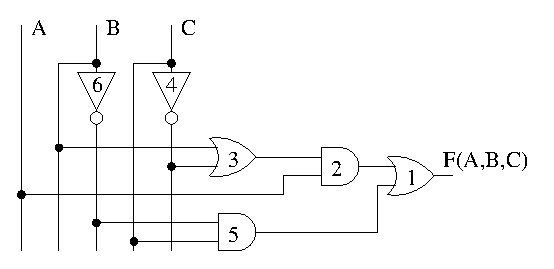
\includegraphics{./Fig2/advance}}
\caption{The circuit diagram for $F(A,B,C)=A(B+C')+B'C$.}
\label{fig:advance}
\end{figure}

During the parsing process, it is critically important to keep track of which 
parts of the expressions have been realized and which have not.  To 
do this, add lines under each of the subexpressions as they are created.
After correctly parsing the expression, each variable should have a little
line underneath it.  This parsing-management can be a dizzying process 
jumping between different levels of the parsing process to resume 
parsing pieces of the expression left unrealized.

\subsection{Symbolic to Symbolic}
The laws of ``regular" algebra are used to discover relationships
between expressions, and to manipulate expressions into more convenient forms.  
Boolean Algebra has a set of laws which can be employed to manipulate 
symbolic expressions.  The nine laws of Boolean Algebra are listed in 
Table~\ref{table:laws}.

\begin{table}
\begin{center}
\begin{tabular}[ht]{|c|c|c|}\hline
Law	&	Primary &	Dual	\\ \hline
1.	&	x+0=x	&	x*1=x	\\ \hline
2.	&	x+1=1	&	x*0=0	\\ \hline
3.	&	x+x=x	&	x*x=x	\\ \hline
4.	&	x''=x	&	     	\\ \hline
5.	&	x+x'=1		& x*x'=0	\\ \hline
6.	&	x+y=y+x		& x*y=y*x\\ \hline
7.	&	x+(y+z)=(x+y)+z	& x*(y*z)=(x*y)*z \\ \hline
8.	&	x*(y+z)=x*y+x*z	& x+(y*z)=(x+y)*(x+z)  \\ \hline
9.	&	(x+y)'=x'*y'  	& (x*y)'=x'+y' \\ \hline
\end{tabular}
\caption{The laws of Boolean Algebra using the Boolean variables $x,y,x$.}
\label{table:laws}
\end{center}
\end{table}

Notice that all laws (except Number 4) have a dual.  A dual of a 
symbolic expression is formed by swapping all ANDs and ORs and all 0s 
and 1s.  Boolean Algebra expresses the 
{\it duality principle}: \index{duality principle}
If a statement $S$ is true, then the dual of $S$ is 
also true. Later, it will be convenient to identify which law is used
to manipulate a symbolic expression.  In these cases, write
down the law's number followed by D if it is a dual.  For example, if 
the property $x*x=x$ is used to manipulate a symbolic expression, then
indicate that Law 3D was used to manipulate the symbolic expression.

The laws in Table~\ref{table:laws} can be verified as true
by plugging in every possible combination of bits and checking if the two sides
of the equation are equal.  For example, to check Law 3D, set $x=0$, 
yielding $0*0=0$ which is true, and then set $x=1$ and verify that $1*1=1$.

The laws of Boolean Algebra can be used to prove two symbolic expressions are 
equal.  This proof is performed by manipulating one of the expressions until it
exactly equals the other side.  For example, to prove that $A + A'B' = A + B'$,
transform the more complex expression into the simpler
expression.  In the example, $A+A'B'$ is the more complex expression and $A+B'$
is the simpler expression.  At each step of the transformation 
provide the law used to yield the next step.

\begin{tabular}[ht]{ll}
$A + A'B' =$		& Law 8D \\
$(A+A')*(A+B')=$	& Law 5 \\
$1*(A+B')=$ 		& Law 1D \\
$A+B'$ \\
\end{tabular}

Working on these derivations is a little like solving a maze or playing
a good game of chess.  Both require a player to ``look ahead" and see what the 
implications of a decision will be.  Not looking far enough ahead may
result in arriving at one of the preceding steps.  For example, consider what 
happened in the following loopy-derivation of $A(A+B)=A$.  The correct 
derivation is shown on the right.

\begin{tabular}[ht]{ll|ll}
Loopy		&		& Correct	&		\\ \hline
$A(A+B)=$ 	& Law 8	& $A(A+B)=$ & Law 8	\\ 
$AA + AB=$ 	& Law 3D	& $A*A+A*B=$& Law 3	\\ 
$A+AB=$	& Law 8D	& $A+A*B$ 	& Law 1D	\\ 
$(A+A)(A+B)=$& Law 3	& $A*1+A*B$	& Law 8	\\ 
$A(A+B)$	& huh?	& $A(1+B)$	& Law 2	\\
		&		& $A(1)$	& Law 1D	\\
		&		& $A$		& \\
\end{tabular}

The {\it expansion trick} can be used to show that two expressions are 
equal to one another.
\index{trick!expansion}  The first step in the expansion trick is
to remove all the parenthesis using Law 8 and reduce the expression
to a set of product terms ORed together. The second step in the 
expansion trick is to add the ``missing" variables to each product 
in the expression.  This second step is illustrated in the following
derivation.

{\bf Show:} $A'B'C' + B'C + ABC = A'B' + AC$

{\bf Derivation:} 

$\begin{array}[ht]{ll}
A'B'C' + B'C + ABC =		& {\rm Law\ 1D} \\
A'B'C' + 1B'C + ABC = 		& {\rm Law\ 3} \\
A'B'C' + (A+A')B'C + ABC = 	& {\rm Law\ 8} \\
A'B'C' + AB'C +A'B'C + ABC = 	& {\rm Law\ 6} \\
A'B'C' + A'B'C +AB'C + ABC = 	& {\rm Law\ 8} \\
A'B'(C' + C) +AC(B' + B) = 	& {\rm Law\ 5} \\
A'B'1 +AC1 = 			& {\rm Law\ 1D} \\
A'B' +AC = 				&  \\
\end{array}$

Since both expressions consist of product terms, Law 8 need not be applied.
 The second step of the expansion trick,
adding the missing variable occurs when $B'C$ is expanded 
into $A'B'C + AB'C$.  In this case, the $B'C$ product term is 
``missing" the $A$ variable.  It is included by first ANDing 1 
with $B'C$, then replacing 1 with $(A+A')$, and finally
distributing $B'C$.  

Finishing this formal derivation is 
straightforward, but requires some scratch work.  Start by 
expanding the right-hand side of the derivation $A'B' + AC$,
using the expansion trick, into $A'B'C' + AB'C +A'B'C + ABC$ 
on some scratch paper.  Now, 
write the second to last step of the scratch work derivation underneath 
the $A'B'C' + AB'C +A'B'C + ABC$ expression in the formal 
derivation.  Then, write the third to last step of the scratch 
work derivation as the next step of the formal derivation.
Continue until $A'B'+AC$ is written as the last step in
the formal derivation.  This idea is similar to a common maze-solving 
strategy, work at both ends of the maze and try to meet 
in the middle. 

The expansion trick runs into problems when there are a large
number of terms in parenthesis.  With a large number
of terms in parenthesis, the distribution process becomes tedious
and error prone. The following derivation utilizes Laws
4 and 9 to avoid this problem.

{\bf Show:} $(A+B)(A'+B)(B+C) = B$

{\bf Derivation:}

$\begin{array}[ht]{ll}
(A+B)(A'+B)(B+C) = 			& {\rm Law\ 4} \\
\left[ (A+B)(A'+B)(B+C) \right] '' =& {\rm Law\ 9D} \\
\left[ (A+B)'+(A'+B)'+(B+C)' \right]' = & {\rm Law\ 9} \\
\left[ A'B'+AB'+B'C' \right]' = 	& {\rm Law\ 8} \\
\left[ B'(A'+A)+B'C' \right]' = 	& {\rm Law\ 5} \\
\left[ [B'1+ B'C' \right]' = 		& {\rm Law\ 1D} \\
\left[ B'(1+C') \right]' = 		& {\rm Law\ 2} \\
\left[ B'1 \right]' = 			& {\rm Law\ 1} \\
\left[ B' \right]' = 			& {\rm Law\ 4} \\
B  &  
\end{array}$

The first step in the derivation, double negating the expression, establishes 
the conditions for the application of Law 9D. One of the negations is
pulled into the bracketed expression converting the product into 
the OR of each product term, negated.  As shown, Law 9 can be applied
to an expression with more than two terms.  In the next step, Law 9 is 
applied to each term in parenthesis.  What remains is a set of product 
terms inside the brackets.  Over the next five steps this product term 
is simplified.  In the final step, the second negation introduced 
back in the first step of the proof is combined with the $B'$ 
inside the brackets, yielding the desired result.

\subsection{Truth Table to Symbolic}
\label{sec:TTtoSymb}

The most technical transformation in the design process is transforming 
a truth table to symbolic expression.  The idea behind this conversion is 
captured by the following analogy.  Imagine eight members of the college 
cheer squad, each have a number between $0 \ldots 7$ pinned to his/her
uniform, are gathered together.  Whenever members of the squad hears
the number pinned to their uniform they give a cheer.  If a member hears
any other number, they do nothing, even if someone else is cheering like crazy.

In order to get a cheer whenever 1, 4, 6, or 7 was announced 
over the public address system, which members of the squad should be
selected?  Clearly, four members of the squad would be selected, the member
with number 1, the member with number 4, the member with number 6,
and the member with number 7.

The squad members in this analogy are circuit elements called 
{\it minterms}. \index{minterm!definition} A minterm for a function 
is a Boolean expression evaluating to logic 1 for a single 
combination of the inputs and evaluates to logic 0 for every 
other input.  A cheering squad member corresponds to a minterm with 
an output of 1.  The number pinned to each squad member corresponds
to the binary input which causes the minterm to output 1.  In order 
to build a symbolic expression for a truth table, first select the
minterms corresponding to the inputs where the function equals 1.  
Next, OR together these minterms and label the output of
the OR gate with the function.  In the cheer squad analogy, the ability of
sound from any member of the cheer squad to be heard corresponds
to the OR gates.  

\paragraph{Minterms}
Up till now minterms have been abstract entities, albeit with
well-defined properties.  To change that, consider all
the minterms for a function  with three input variables 
$A,B,C$.  Since $F$ has eight different inputs, it will have eight 
minterms.  Next, build the minterm that ``recognizes" the input $A=B=C=1$.  
This task is accomplished by creating an expression which outputs 1 only when 
$A=B=C=1$.  In this case, the minterm is $ABC$ because it equals 
1 when all the inputs are 1, and for any other input, a 0.
This minterm is denoted $m_7$, the lowercase $m$ signifies that 
this is a minterm and the 7 denotes the decimal representation 
of the input which causes this minterm to equal 1.  

The minterm
for the input $A=0, B=1, C=0$, $m_2$, is $A'BC'$.  Negating the
$A$ and $C$ variables allows a 0 input value for these variables to 
be inverted to 1 before being ANDed.  

In order to make generating 
the remaining six minterms easier, formalize the observation 
just made and call it the {\it minterm trick}.  
\index{trick!minterm} \label{page:MinTrick}
A minterm for a particular input needs to include all the variables.
If a variable's value is equal to 0, the variable should be negated in 
the AND expression, if its value is 1, it appears as itself in the
AND expression. The table below shows all the minterms for three 
variables A,B,C.

\begin{tabular}{c|c|c||c|c}
A & B & C & minterm & symbol	\\ \hline
0 & 0 & 0 & A'B'C'  & $m_0$	\\ \hline
0 & 0 & 1 & A'B'C   & $m_1$	\\ \hline
0 & 1 & 0 & A'BC'   & $m_2$	\\ \hline
0 & 1 & 1 & A'BC    & $m_3$	\\ \hline
1 & 0 & 0 & AB'C'   & $m_4$	\\ \hline
1 & 0 & 1 & AB'C    & $m_5$	\\ \hline
1 & 1 & 0 & ABC'    & $m_6$	\\ \hline
1 & 1 & 1 & ABC     & $m_7$	\\ 
\end{tabular}

A minterm is said to ``recognizes its input" when that input
causes the minterm to evaluate to 1.  Thus, minterm $m_3$ recognizes
the input $(A,B,C)=(0,1,1)$ and ignores all other inputs.  In order 
to construct the symbolic expression for a truth table, OR together 
the minterms for which the function equals 1. Thus, when any one of 
the minterms recognizes its input, one of the inputs to the OR gate 
will equal 1 causing the output of the OR gate to become 1.  Note, 
that at most one of the OR gates inputs will equal 1, since only one 
of the minterms will recognize its input.  If none of the minterms 
recognizes the input, all the inputs of the OR gate will equal 0, 
causing the output of the OR gate to equal 0.  To better understand
these concepts, consider the function $F(A,B,C)$ defined below.

\begin{tabular}{c|c|c||c|c|c}
A & B & C & F(A,B,C)	& minterm & symbol	\\ \hline
0 & 0 & 0 & 0		& A'B'C'  & $m_0$	\\ \hline
0 & 0 & 1 & 1		& A'B'C   & $m_1$	\\ \hline
0 & 1 & 0 & 1		& A'BC'   & $m_2$	\\ \hline
0 & 1 & 1 & 1		& A'BC    & $m_3$	\\ \hline
1 & 0 & 0 & 1		& AB'C'   & $m_4$	\\ \hline
1 & 0 & 1 & 0		& AB'C    & $m_5$	\\ \hline
1 & 1 & 0 & 0		& ABC'    & $m_6$	\\ \hline
1 & 1 & 1 & 1		& ABC     & $m_7$	\\ 
\end{tabular}
\\ \\
There are five inputs for which $F(A,B,C)$ equals 1, so the symbolic
expression for $F$ will include the five minterms from the rows where
$F$ equals 1.  Hence, 
$$F(A,B,C) =  A'B'C + A'BC' + A'BC + AB'C' + ABC$$
Now, examine what happens to $F$ for the input $(A,B,C)=(0,0,1)$.  
The minterm $m_1=A'B'C$ evaluates to 1 while all the other minterms 
evaluate to 0.  Since the OR function evaluates to 1 when any of 
the inputs are equal 1, $F$ equals to 1. Hence, $F(0,0,1)=1$ as
expected.  When $(A,B,C)=(1,1,0)$ is applied, all the
minterms in the symbolic expression for $F$ evaluate to 0 because
none of them recognize this input.  Thus, $F(1,1,0)=0$ as expected.

When a function is constructed by ORing together minterms, it is
said to be in {\it canonical sum of products} 
\index{SOP!canonical} form or canonical SOP form.  A symbolic
expression is said to be in SOP form when it consists
exclusively of a collection of product terms ORed together.  
The term sum/product is used to refer to the operators OR/AND 
respectively because these are what the operators look like in 
normal arithmetic. The term canonical is used because this 
symbolic form is the most elementary form possible to describe 
the function.

The canonical SOP representation for $F$ defined above can be 
abbreviated as $F(A,B,C) = \sum m(1,2,3,4,7)$  where the $\sum$
symbol denotes the ORing together of minterms 1,2,3,4 and 7.
In general, $\sum m(list)$ describes the inputs for which the
function equals 1.  When asked for a canonical SOP expression
in the homework, write either the symbolic expression
out, or use this abbreviated form.

Engineers are always striving to minimize the cost of their solutions.
Towards this end, a second way to transform a truth table into a 
symbolic expression is introduced.  It replaces the minterms with 
a different kind of building block, the maxterm.

\paragraph{Maxterms}
\index{maxterm!definition}
A {\it maxterm} for a function is a symbolic expression evaluating
to 0 for a single combination of the inputs and evaluates to 1 for 
every other input.  Before constructing symbolic expressions for
a truth table, it is necessary to examine the structure of maxterms.

Since the function $F(A,B,C)$ has three inputs, it will have eight 
maxterms.  Start by creating the maxterm for the input $(A,B,C)=(0,0,0)$.
Many different expressions can be derived which equal 0 only for
this input, but the simplest is $A+B+C$.  This maxterm is
abbreviated $M_0$, the uppercase $M$ signifying a maxterm 
and the 0 denoting the decimal representation of the input which 
causes this maxterm to equal 0.  The {\it maxterm trick} 
\index{trick!maxterm} is used to simplify the process of creating
maxterms.  

A maxterm for a particular input needs to include all the variables.
If a variable's value is equal to 1, the variable should be negated 
in the OR expression; if its value is 0, the expression appears as itself in the
OR expression. The table below lists all the maxterms for the three 
variables $A,B,C$.

\begin{tabular}{c|c|c||c|c}
A & B & C & maxterm   & symbol \\ \hline
0 & 0 & 0 & A+B+C     & $M_0$   \\ \hline
0 & 0 & 1 & A+B+C'    & $M_1$   \\ \hline
0 & 1 & 0 & A+B'+C    & $M_2$   \\ \hline
0 & 1 & 1 & A+B'+C'   & $M_3$   \\ \hline
1 & 0 & 0 & A'+B+C    & $M_4$   \\ \hline
1 & 0 & 1 & A'+B+C'   & $M_5$   \\ \hline
1 & 1 & 0 & A'+B'+C   & $M_6$   \\ \hline
1 & 1 & 1 & A'+B'+C'  & $M_7$   \\ 
\end{tabular}


In order to construct the symbolic expression for a truth table, 
AND together the maxterms for which the function equals 0. Thus, 
when any one of the maxterms recognizes its input, one of the 
inputs to the AND gate will equal 0, causing the output of the 
AND gate to go to 1.  Note, that at most one of the AND gate's 
inputs will equal 0, since only one of the maxterms will recognize 
the input.  If none of the maxterms recognizes the input, all the 
inputs of the AND gate equal 1, causing the output of the 
AND gate to equal 1.  These ideas are applied to 
the function $F(A,B,C)$ below.

\begin{tabular}{c|c|c||c|c|c}
A & B & C & F(A,B,C) & maxterm   & symbol \\ \hline
0 & 0 & 0 & 0        & A+B+C     & $M_0$   \\ \hline
0 & 0 & 1 & 1        & A+B+C'    & $M_1$   \\ \hline
0 & 1 & 0 & 1        & A+B'+C    & $M_2$   \\ \hline
0 & 1 & 1 & 1        & A+B'+C'   & $M_3$   \\ \hline
1 & 0 & 0 & 1        & A'+B+C    & $M_4$   \\ \hline
1 & 0 & 1 & 0        & A'+B+C'   & $M_5$   \\ \hline
1 & 1 & 0 & 0        & A'+B'+C   & $M_6$   \\ \hline
1 & 1 & 1 & 1        & A'+B'+C'  & $M_7$   \\ 
\end{tabular}
\\ \\
There are three inputs of $F(A,B,C)$ equal to 0, so the symbolic
expression for $F$ includes the three maxterms from the rows where
$F$ equals 0.  Hence, 

$$F(A,B,C) =  (A+B+C)(A'+B+C')(A'+B'+C)$$

What happens when the input $(A,B,C)=(1,0,1)$ is applied?  
The maxterm $M_5=(A'+B+C')$ evaluates to 0 while all the other maxterms 
evaluate to 1.  Since the AND function evaluates to 0 when any of 
the inputs are equal 0, $F$ equals to 0. Hence, $F(1,0,1)=0$ as
expected.  When $(A,B,C)=(1,1,1)$ is applied, all the
maxterms in the symbolic expression for $F$ evaluate to 1 because
none of them recognize this input.  Thus $F(1,1,1)=1$ as expected.

\index{POS!canonical}
This representation of $F$ is called its {\it canonical product of sums} 
form or canonical POS form, because $F$ is represented in its most
elementary form as the AND (product) of a collection of OR (sum) terms.  
The canonical POS representation in the example can be abbreviated by 
the expression $F(A,B,C) = \prod M(0,5,6)$  where the $\prod$
symbol denotes the AND, the $M$ symbol stands for maxterm, and the 
numbers in the list are the inputs for which $F(A,B,C)$ equals 0.

Notice, the functions in the two minterm and maxterm examples are the 
same.  This was done to illustrate two points.  First, the inputs 
present in the minterm list are those that do not appear in the maxterm 
list.  In other words, $F(A,B,C) = \sum m(1,2,3,4,7) = \prod M (0,5,6)$.  
This should make sense. The minterm list denotes those inputs for 
which the function equals 1.  If the function does not equal 1 for 
a particular input, this input is not in the minterm list, and then the 
function must equal 0 for this input, hence this input will appear 
in the maxterm list.

The second reason for using the same function is to illustrate
how different realizations of the same function have different costs.
A solution requiring fewer gates
will cost less.  The following table summarizes the number of gates 
required in the SOP and POS realization of $F(A,B,C)$.
\\ \\
\begin{tabular}[ht]{l|c|c}
		    & SOP 	& POS	\\ \hline
 number of NOTs & 3	& 3	\\ \hline
 number of ANDs & 5	& 1	\\ \hline
 number of ORs  & 1	& 3	\\ 
\end{tabular}
\\ \\
Assuming that AND gates and OR gates have the same cost then the POS 
solution costs less.  Thus a good engineer would recommend a 
canonical POS realization over a canonical SOP realization.

While, the transformation from a truth table to a symbolic expression
may be the most technically challenging, it is certainly not the
most difficult.  This title belongs to the transformation of a word
statement into a truth table.  The difficulty of this transformation
has its origin in the puffy cloud outline of a word statement shown in
Figures \ref{fig:Design} \ref{fig:forms}. Words can be ambiguous and 
the ability of authors to convey precisely what the digital system
needs to accomplish depends on their skill with the English language.

\subsection{Word Statement to Truth Table}
There is no algorithmic approach guaranteed to transform a word statement 
into a truth table.  That said, the following list outlines essential
information to obtain from the word statement in order to
have any hope of transforming it into a truth table.

\begin{description}
\item [Step 1] Understand the number and meaning of the
inputs and the outputs of the digital system.  The meaning of inputs
will vary from system to system.  Typically, the inputs are broken into
collections of bits.  Each collection will have its own meaning attached
to it.

\item [Step 2] Write down an empty truth table.  If
the digital system has $N$ bits of input, then the truth table
has $2^N$ rows.  

\item [Step 3] Use the word statement to determine the output for 
each input, one row at a time.  This requires understanding what the inputs 
and outputs mean and then determining the relationship between each
input and output pair.
\end{description}

The following example shows how to apply these steps to a word statement.

\begin{quote}
Determine the truth table for 
a function with two bits of input and one bit of output.  The
output equals 1 when all the inputs are equal to 1.
\end{quote}

The 3-step process for transforming a word statement into a 
truth table are shown below.

\begin{description}
\item [Step 1] The function has two bits of input and one bit of output.  
Since the inputs and output were not given names, use the default labels
$A,B$ for the inputs and $F$ for the output.

\item [Step 2] The truth table for a 2-variable function has four 
rows.

	\begin{tabular}{c|c||c}
	A & B & F \\ \hline \hline
	0 & 0 &   \\ \hline
	0 & 1 &   \\ \hline
	1 & 0 &   \\ \hline
	1 & 1 &   \\
	\end{tabular}

\item [Step 3] The only row of the truth table where $A$ and $B$ both
equal to 1 is the last row; set this row's output equal to 1.  
All the other rows of the table have $F=0$ because they have
at least one input which equals 0.

	\begin{tabular}{c|c||c}
	A & B & F \\ \hline \hline
	0 & 0 & 0  \\ \hline
	0 & 1 & 0  \\ \hline
	1 & 0 & 0  \\ \hline
	1 & 1 & 1  \\
	\end{tabular}
\end{description}

This should be recognizable as the AND function.  In the
AND example, each of the bits was a distinct input by itself.  
Sometimes, the inputs work together to form some larger unit of
information, like a binary number.  This is the case in the next
example.

\begin{quote}
Determine the truth table for a function with three bits of input and
one bit of output.  The output of the function should equal 1 when
the 3-bit binary input represents a binary number greater than 4.
\end{quote}

\begin{description}
\item [Step 1] The function has three bits of input and one bit of output.  
Since the inputs and outputs were not given names, use the default labels
$a_2,a_1,a_0$ for the inputs and $F$ for the output.  The input
variables are given subscripts because they are working together to 
form a 3-bit binary number.  The binary number is referred to as
$A$ and its individual bits as $a_2$, $a_1$, and $a_0$.  Hence,
when $(a_2,a_1,a_0) = (1,0,1)$ then $A=5$.

\item [Step 2] Many 3-variable truth tables have been shown in this
chapter.  The notable point in this example is that the output is 
abbreviated as $F(A)$ to save space.

$\begin{array}[ht]{l|l|l||l}
a_2 & a_1 & a_0 & F(A)		\\ \hline
0   & 0   & 0   &		\\ \hline
0   & 0   & 1   &		\\ \hline
0   & 1   & 0   &		\\ \hline
0   & 1   & 1   &		\\ \hline
1   & 0   & 0   &		\\ \hline
1   & 0   & 1   &		\\ \hline
1   & 1   & 0   &		\\ \hline
1   & 1   & 1   &		\\ 
\end{array}$

\item [Step 3] The output of the function equals 0 for all inputs
less than or equal to $(a_2,a_1,a_0) = (1,0,0)$ and equals 1 for 
inputs greater or equal to $(a_2,a_1,a_0) = (1,0,1)$.  This yields
the following truth table.

$\begin{array}[ht]{l|l|l||l}
a_2 & a_1 & a_0 & F(A)		\\ \hline
0   & 0   & 0   &	0	\\ \hline
0   & 0   & 1   &	0	\\ \hline
0   & 1   & 0   &	0	\\ \hline
0   & 1   & 1   &	0	\\ \hline
1   & 0   & 0   &	0	\\ \hline
1   & 0   & 1   &	1	\\ \hline
1   & 1   & 0   &	1	\\ \hline
1   & 1   & 1   &	1	\\ 
\end{array}$

\end{description}

In the third and final example, there are two twists.  The truth
table will describe a function with four variables and the function
has three bits of output.  For the sake of brevity, the second and the 
third steps of the transformation process are combined.

\begin{quote}
Determine the truth table for a digital system having two, 2-bit 
inputs $A=a_1 a_0$ and $B=b_1 b_0$. Each 2-bit input represents a 
2-bit binary number.  The function has three bits of output called
$G$, $L$, and $E$, which stand for greater, less, and equal, respectively.
$E$ equals 1 when $A=B$, $G=1$ when $A>B$, and $L=1$ when $A<B$.
\end{quote}

\begin{description}
\item [Step 1] The function has four bits of input and three bits of output.
The names of these variables are clear from the word statement.

\item[Step 2 \& 3]  The truth table for this function has 16 rows
because there are $2^4=16$ combinations of four bits 
(see page~\pageref{page:two-to-N}).
In order to better visualize the solution to the problem, the values of $A$ and
$B$ (derived from their values of $a_1,a_0$ and $b_1,b_0$) are included 
in the truth table.  

$$\begin{array}{c|c|c|c||c|c||c|c|c}
a_1 & a_0 & b_1 & b_0 & A & B & G & L & E \\ \hline
0 & 0 & 0 & 0 & 0 & 0 & 0 & 0 & 1  \\ \hline
0 & 0 & 0 & 1 & 0 & 1 & 0 & 1 & 0  \\ \hline
0 & 0 & 1 & 0 & 0 & 2 & 0 & 1 & 0  \\ \hline
0 & 0 & 1 & 1 & 0 & 3 & 0 & 1 & 0  \\ \hline
0 & 1 & 0 & 0 & 1 & 0 & 1 & 0 & 0  \\ \hline
0 & 1 & 0 & 1 & 1 & 1 & 0 & 0 & 1  \\ \hline
0 & 1 & 1 & 0 & 1 & 2 & 0 & 1 & 0  \\ \hline
0 & 1 & 1 & 1 & 1 & 3 & 0 & 1 & 0  \\ \hline
1 & 0 & 0 & 0 & 2 & 0 & 1 & 0 & 0  \\ \hline
1 & 0 & 0 & 1 & 2 & 1 & 1 & 0 & 0  \\ \hline
1 & 0 & 1 & 0 & 2 & 2 & 0 & 0 & 1  \\ \hline
1 & 0 & 1 & 1 & 2 & 3 & 0 & 1 & 0  \\ \hline
1 & 1 & 0 & 0 & 3 & 0 & 1 & 0 & 0  \\ \hline
1 & 1 & 0 & 1 & 3 & 1 & 1 & 0 & 0  \\ \hline
1 & 1 & 1 & 0 & 3 & 2 & 1 & 0 & 0  \\ \hline
1 & 1 & 1 & 1 & 3 & 3 & 0 & 0 & 1  \\ 
\end{array}$$
\end{description}

In order to transform this truth table into a symbolic expression, 
realize each of the three outputs are independent of the
others.  For example, to determine the symbolic expression for $G$,
cover-up the output columns corresponding to the $L$ and $E$ outputs
and implement $G$.  In order to realize $L$, just cover-up the 
columns associated with $G$ and $E$ and implement $L$ as if
the other two outputs did not exist.  This yields the following
three equations for the outputs.

$$\begin{array}{l}
G(a_1,a_0,b_1,b_0)=\sum m(4,8,9,12,13,14)	\\
L(a_1,a_0,b_1,b_0)=\sum m(1,2,3,6,7,11)	\\
E(a_1,a_0,b_1,b_0)=\sum m(0,5,10,15)	\\
\end{array}$$

Of course this leads to the question of how to build the circuit
diagram for this 4-input, 3-output function.  Students often
want to OR together the $G$, $L$, and $E$ outputs in order to have
a single output, but this is would be incorrect because the word 
statement asked for three separate outputs.  The correct way to build
the circuit diagram is to build each of the circuits separately, give
each its own output, and have them share the same inputs.  A rough
sketch of the circuit is shown in Figure~\ref{fig:ThreeOutputs}.

\begin{figure}[ht]
\center{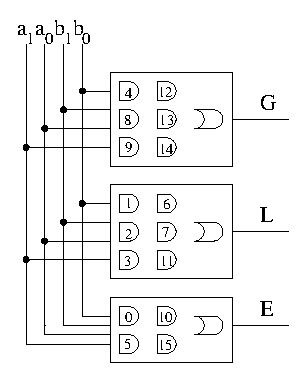
\includegraphics{./Fig2/ThreeOutputs}}
\caption{The circuit diagram for a circuit which compares the 
magnitude of the two inputs $A=a_1 a_0$ and $B=b_1 b_0$.  Many of 
the internal details have been omitted.}
\label{fig:ThreeOutputs}
\end{figure}

Notice that the three output circuits share the same inputs, but otherwise
are independent of one another.  Sharing inputs allows each
circuit to coordinate its output with the other circuits.  When
each circuit does what it is supposed to do for that input, the
output looks like a unified whole even though it is generated from
three separate circuits.

\section{Timing Diagrams}
\index{timing!diagrams}
After a circuit has been realized in hardware, the logical
representation of 0s and 1s is replaced by physical voltages
representing these logic levels.  In order to observe the behavior
of a physical digital system, an engineer typically uses a
logic analyzer or oscilloscope.  The waveforms drawn by the logic
analyzer when applying inputs and examining the outputs is called
a {\it timing diagram}.  A timing diagram is a graph of the logic value 
of a signal versus time.  Typically, several signals are combined on the
same timing diagram to save space and in order to clearly 
show the relationship between the signals.

It is imperative to check if the digital system implemented
behaves according to its specification. Hence, an understanding of
timing diagrams is essential.  With a small circuit it is reasonable
to apply every possible combination of inputs and examine the 
output of the circuit.  For example, Figure~\ref{fig:time} shows
the timing diagram for $F(A,B,C) = A'B+AB'C$.

\begin{figure}[ht]
\center{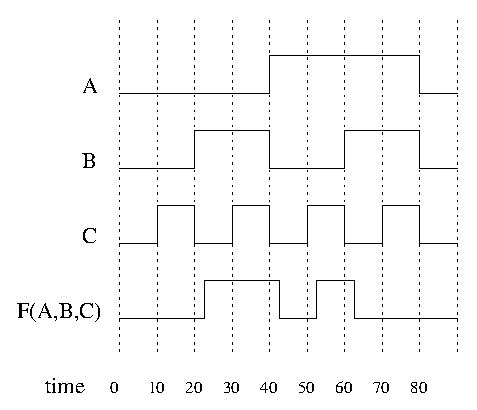
\includegraphics{./Fig2/time}}
\caption{A timing diagram for $F(A,B,C) = A'B + AB'C$.}
\label{fig:time}
\end{figure}

Observe that the time intervals are spaced 10 units apart.  For
now, the meaning of the units is unimportant.  Most likely, they would
be nanoseconds.  In practice, the timing behavior of a circuit
may be very important because circuits must not only have the 
correct output, but the circuit must meet strict timing constraints.

At time=5 the input $(A,B,C)=(0,0,0)$ and the output in response
to this input is 0.  At time=15 the input is $(0,0,1)$, and the
output due to this input is 0.  At time=75 the input is $(1,1,1)$
and the output is 0.  Every combination of the inputs has been 
applied to the circuit allowing the test engineer to verify the 
functional behavior of the circuit.

\subsection{Propagation Delay}
Notice that when the inputs change at time=20, the output $F$ 
transitions from 0 to 1 a little after time=20. This delay in the 
output transition is a manifestation of a real physical effect 
called {\it propagation delay}.  
\begin{quote}
Propagation delay is the time difference between the application of 
inputs and when the outputs becoming valid. 
\end{quote}
The physical basis of propagation delay is due to the finite amount 
of time required to charge or discharge a capacitor.  Propagation delay
is a limiting factor in processor speeds and has been know to cause
logical errors in circuit behavior.  It is so important that parts vendors
state the propagation delays of their circuits.  For example, 
consulting the technical documents for the Texas Instruments
74LS32, an OR gate, reveals four different values for propagation
delay: A typical, and a maximum value for both \Tphl and \Tplh.

\begin{tabular}{c|c|c}
         & TYPICAL & MAX  \\ \hline
\Tplh    & 10nS    & 15nS \\ 
\Tphl    & 14nS    & 22nS \\
\end{tabular}
\\ \\
\Tphl stands for the propagation delay to switch the output from
logic 1 to logic 0.  Likewise, \Tplh stands for the propagation delay 
to switch the output from 0 to 1. The TYPICAL and MAX columns 
give the tolerances the manufacture guarantees.  To simplify
analysis, the largest maximum delay can be used as a single value
for the propagation delay.  For example, it is safe to assume that
the outputs of a 74LS32 will switch in 22nS. 

\subsection{Hazards}
\pagebreak
.
\pagebreak
.

\section{VHSIC Hardware Description Language}
\pagebreak
.
\subsection{Entity and Architecture}
\pagebreak
.
\pagebreak
.
\subsection{Concurrent Signal Assignment Statements}
\pagebreak
.
\pagebreak
.

\section{Exercises}
\section{Exercises}
\label{section:representationsExercises}
\graphicspath{ {./chapter02/FigHw} }

\begin{enumerate}
\item \textbf{(2 pts. each)} Given: $F(A,B,C,D) = (AB' + (C+(AD)')(BD))'$

\begin{enumerate}
	\item Determine the truth table for $F(A,B,C,D)$

\begin{onlysolution}  \textbf{Solution} \itshape

Let T3 = C+(AD)'\\
T4 = BD\\
T1 = AB'
T5 = T3 * T4\\

\begin{tabular}{l|l|l|l|l|l|l|l|l|l|l} 
 A &  B &  C &  D & AB' & (AD)' & C+(AD)' & BD & T3*T4 & T1+T5  &  F \\ \hline
 0 &  0 &  0 &  0 &  0  &  1    &  1      &  0 & 0     &  0     &  1  \\ \hline
 0 &  0 &  0 &  1 &  0 &  1 &  1 &  0 & 0 &  0 &  1  \\ \hline
 0 &  0 &  1 &  0 &  0 &  1 &  1 &  0 & 0 &  0 &  1  \\ \hline
 0 &  0 &  1 &  1 &  0 &  1 &  1 &  0 & 0 &  0 &  1  \\ \hline
 0 &  1 &  0 &  0 &  0 &  1 &  1 &  0 & 0 &  0 &  1  \\ \hline
 0 &  1 &  0 &  1 &  0 &  1 &  1 &  1 & 1 &  1 &  0  \\ \hline
 0 &  1 &  1 &  0 &  0 &  1 &  1 &  0 & 0 &  0 &  1  \\ \hline
 0 &  1 &  1 &  1 &  0 &  1 &  1 &  1 & 1 &  1 &  0  \\ \hline
 1 &  0 &  0 &  0 &  1 &  1 &  1 &  0 & 0 &  1 &  0  \\ \hline
 1 &  0 &  0 &  1 &  1 &  0 &  0 &  0 & 0 &  1 &  0  \\ \hline
 1 &  0 &  1 &  0 &  1 &  1 &  1 &  0 & 0 &  1 &  0  \\ \hline
 1 &  0 &  1 &  1 &  1 &  0 &  1 &  0 & 0 &  1 &  0  \\ \hline
 1 &  1 &  0 &  0 &  0 &  1 &  1 &  0 & 0 &  0 &  1  \\ \hline
 1 &  1 &  0 &  1 &  0 &  0 &  0 &  1 & 0 &  0 &  1  \\ \hline
 1 &  1 &  1 &  0 &  0 &  1 &  1 &  0 & 0 &  0 &  1  \\ \hline
 1 &  1 &  1 &  1 &  0 &  0 &  1 &  1 & 1 &  1 &  0  \\  
\end{tabular} 
\end{onlysolution}

	\item Draw a schematic of the logic circuit which realizes $F$ as
	shown, i.e. do not use Boolean Algebra on $F$.

\begin{onlysolution}  \textbf{Solution} \itshape
	\begin{figure}[ht]
	\includegraphics{Sol2-1}
	\end{figure}
\end{onlysolution}
\end{enumerate}


\item \textbf{(2 pts. each)} For the circuit in Figure~\ref{fig:representationsHwCir2Bool}
\begin{enumerate}
	\item Write a Boolean expression for the function.

	\begin{onlysolution}  \textbf{Solution} \itshape 
	F(A,B,C,D) = (AB+C)D'+ABD'\end{onlysolution}
	
\item Draw the truth table for the function.


	\begin{onlysolution}  \textbf{Solution} \itshape
	
	\begin{tabular}{l|l|l|l|l|l|l|l}
	 A &  B &  C &  D & AB+C  & (AB+C)D' & ABD'  &  F  \\ \hline
	 0 &  0 &  0 &  0 &  0 &  0 &  0 &  0  \\ \hline
	 0 &  0 &  0 &  1 &  0 &  0 &  0 &  0  \\ \hline
	 0 &  0 &  1 &  0 &  1 &  0 &  0 &  1  \\ \hline
	 0 &  0 &  1 &  1 &  1 &  1 &  0 &  0  \\ \hline
	 0 &  1 &  0 &  0 &  0 &  0 &  0 &  0  \\ \hline
	 0 &  1 &  0 &  1 &  0 &  0 &  0 &  0  \\ \hline
	 0 &  1 &  1 &  0 &  1 &  0 &  0 &  1  \\ \hline
	 0 &  1 &  1 &  1 &  1 &  1 &  0 &  0  \\ \hline
	 1 &  0 &  0 &  0 &  0 &  0 &  0 &  0  \\ \hline
	 1 &  0 &  0 &  1 &  0 &  0 &  0 &  0  \\ \hline
	 1 &  0 &  1 &  0 &  1 &  0 &  0 &  1  \\ \hline
	 1 &  0 &  1 &  1 &  1 &  1 &  0 &  0  \\ \hline
	 1 &  1 &  0 &  0 &  1 &  0 &  1 &  1  \\ \hline
	 1 &  1 &  0 &  1 &  1 &  1 &  0 &  0  \\ \hline
	 1 &  1 &  1 &  0 &  1 &  0 &  1 &  1  \\ \hline
	 1 &  1 &  1 &  1 &  1 &  0 &  0 &  0  \\ 
	\end{tabular}
\end{onlysolution}
\end{enumerate}
\begin{figure}[ht]
\includegraphics{Prob2-3}
\caption{The circuit for Problems 2 and 3.}
\label{fig:representationsHwCir2Bool}
\end{figure}

\item \textbf{ (2 pts. each)} For the functions F,G,H,I defined by the 
truth table shown below:
\begin{enumerate}
	\item Determine the canonical SOP and POS realization for $F,G,H,I$.

	\begin{onlysolution}  \textbf{Solution} \itshape
	
F(A,B,C) = (A+B+C)(A+B'+C')(A'+B+C')(A'+B'+C)  =
A'B'C + A'BC' + AB'C' + ABC \\

G(A,B,C) = (A'+B+C)(A'+B'+C') = \\
A'B'C' + A'B'C + A'BC' + A'BC + AB'C + ABC'  \\

H(A,B,C) = (A+B'+C)(A+B'+C')(A'+B+C)(A'+B+C')(A'+B'+C') =\\
A'B'C' + A'B'C + ABC' \\

I(A,B,C) = (A+B+C)(A+B'+C)(A'+B+C)(A'+B'+C) =\\
A'B'C + A'BC + AB'C + ABC \\
\end{onlysolution}

	\item Draw the circuit diagram for the canonical SOP and POS 
		realization.

	\begin{onlysolution}  \textbf{Solution} \itshape
	\begin{figure}[ht]
	\includegraphics{Sol2-4}
	\end{figure}
\end{onlysolution}
\end{enumerate}
Treat each output independently of the other.  For example when
working with function $I$, cover up the columns $F,G$ and $H$.

$$\begin{array}{c|c|c||c|c|c|c}
 	A & B & C & F & G & H & I \\ \hline
 	0 & 0 & 0 & 0 & 1 & 1 & 0 \\ \hline
 	0 & 0 & 1 & 1 & 1 & 1 & 1 \\ \hline
 	0 & 1 & 0 & 1 & 1 & 0 & 0 \\ \hline
 	0 & 1 & 1 & 0 & 1 & 0 & 1 \\ \hline
 	1 & 0 & 0 & 1 & 0 & 0 & 0 \\ \hline
 	1 & 0 & 1 & 0 & 1 & 0 & 1 \\ \hline
 	1 & 1 & 0 & 0 & 1 & 1 & 0 \\ \hline
 	1 & 1 & 1 & 1 & 0 & 0 & 1 \\
\end{array}$$

\item  \textbf{ (2 pts. each)} Prove the validity of the following 
statements using the laws of Boolean Algebra. For each step of 
the proof, identify which law was used.
\begin{enumerate}
	\item $X'Y' + XY + X'Y = X' + Y$

\begin{onlysolution}  \textbf{Solution} \itshape

\begin{tabular}{lr}
X'Y' + XY + X'Y = 	& 3D\\
X'Y' + X'Y + XY+ X'Y =	& 8 \\
X'(Y' + Y )+ Y(X+ X')Y=	& 5 \\
X' + Y 			& QED \\
\end{tabular} \end{onlysolution}

	\item $(X+Y')X'Y' = X'Y'$

\begin{onlysolution}  \textbf{Solution} \itshape

\begin{tabular}{lr}
(X+Y')X'Y' = 	& 8 \\
XX'Y + X'Y'Y' = & 5D \\
0+X'Y'= 	& 1 \\
X'Y' 		& QED \\
\end{tabular}\end{onlysolution}

	\item $(X+Y)(X'+Z) = XZ + X'Y$

\begin{onlysolution}  \textbf{Solution} \itshape

\begin{tabular}{lr}
(X+Y)(X'+Z) = 		& 8 \\
(X+Y)X' + (X+Y)Z = 	& 8 \\
XX' + YX' + XZ + YZ =	& 1D,5 \\
YX' + XZ + YZ(X+X') =  	& 8 \\
YX' + XZ + XYZ + X'YZ =	& 6  \\
X'Y + X'YZ + XZ + XYZ =	& 1D, 8 \\
X'Y(1+Z) + XZ(1+Y) =  	& 2, 1D \\
X'Y + XZ 		& QED \\
\end{tabular} \end{onlysolution}

	\item $X'Y' + (X+Y)Z = X'Y' + Z$

\begin{onlysolution}  \textbf{Solution} \itshape

\begin{tabular}{lr}
X'Y' + (X+Y)Z = 				& 8\\
X'Y' + XZ + YZ = 				& 1D,5 \\
X'Y'*(Z+Z') + XZ + YZ(X+X') =  			& 8 \\
X'Y'Z' + X'Y'Z + XZ + XYZ + X'YZ =  		& 3 \\
X'Y'Z' + X'Y'Z + X'Y'Z + XZ + XYZ + X'YZ =  	& 8 \\
X'Y'(Z+Z') + XZ(1+Y) + X'Z(Y'+Y) =  		& 5,1D \\
X'Y' + XZ + X'Z  =  				& 8 \\
X'Y' + Z(X+X') =  				& 5, 1D\\
X'Y' + Z 					& QED \\
\end{tabular} \end{onlysolution}

	\item $A'C+BC+AB = A'C+AB$

\begin{onlysolution}  \textbf{Solution} \itshape

\begin{tabular}{lr}
A'C + BC+AB =  					& 1D, 5 \\
A'C + (A+A')BC + AB(C+C') 			& 8  \\
A'C + ABC + A'BC + ABC + ABC'= 			& 3\\
A'C + A'BC + ABC + ABC'= 			& 8\\
A'C(1+B) + AB(C+C')= 				& 5, 1D\\
A'C + AB 					& QED \\
\end{tabular} \end{onlysolution}
	\item $A(B+C)=AB+AB'C$

\begin{onlysolution}  \textbf{Solution} \itshape

\begin{tabular}{lr}
AB+AB'C= 					& 1D,5\\
AB(C+C') + AB'C= 				& 8 \\
ABC+ABC'+AB'C= 					& 3 \\
ABC + ABC + ABC' + AB'C= 			& 6\\
ABC + ABC' + ABC + AB'C= 			& 8\\
AB(C+C'+C) + AB'C = 				& 8\\	
AB + AB'C= 					& QED\\
\end{tabular}	\end{onlysolution}
	\item $(A+B+C)(A+B+C')(A'+B+C')(A'+B'+C') = (A+B)(A'+C')$

\begin{onlysolution}  \textbf{Solution} \itshape

\begin{tabular}{lr}
(A+B+C)(A+B+C')(A'B+C')(A'+B'+C')= 		& 4\\
((A+B+C)(A+B+C')(A'B+C')(A'+B'+C'))''= 		& 9D\\
(A'B'C + A'B'C' + AB'C + ABC)'= 		& 8\\
(A'B'(C+C') + AC(B'+B))'= 			& 5, 1D\\
(A'B' + AC)'= 					& 9 \\
(A+B)(A'+C')= 					& QED \\
\end{tabular}	\end{onlysolution}
\end{enumerate}

\item \textbf{ (4 pts.)} Design a circuit called MUX2.  MUX2 has three bits 
of input $S, y_0, y_1$ and one bit of output $F$.  If $S=0$, then 
$F=y_0$; else if $S=1$, then $F=y_1$.
\begin{enumerate}
	\item Write down the truth table for the MUX2 function.

\begin{onlysolution}  \textbf{Solution} \itshape

	\begin{tabular}{l|l|l|l}
	S & y0 &  y1 & F \\ \hline
	0 & 0  &  0  & 0 \\ \hline
	0 & 0  &  1  & 0 \\ \hline
	0 & 1  &  0  & 1 \\ \hline
	0 & 1  &  1  & 1 \\ \hline
	1 & 0  &  0  & 0 \\ \hline
	1 & 0  &  1  & 1 \\ \hline
	1 & 1  &  0  & 0 \\ \hline
	1 & 1  &  1  & 1 \\ 
	\end{tabular}
\end{onlysolution}

	\item Determine the canonical SOP realization for MUX2; 
		do not simplify.

\begin{onlysolution}  \textbf{Solution} \itshape 
F = S'y0y1' + S'y0y1 + Sy0'y1 + Sy0y1
\end{onlysolution}
\end{enumerate}

\item \textbf{ (6 pts.)} Design a circuit called MUX4.  MUX4 has six bits of input 
$S_1 S_0, y_0, y_1, y_2, y_3$ and one bit of output $F$.  \\
If      $S_1 S_0 = 00$ then $F=y_0$  \\
else if $S_1 S_0 = 01$ then $F=y_1$ \\
else if $S_1 S_0 = 10$ then $F=y_2$ \\
else if $S_1 S_0 = 11$ then $F=y_3$ \\
Without writing down the truth table determine a SOP expression
to realize F by listing all possible inputs which will cause F to equal 1.
Then try to simplify your expression using Boolean Algebra.

\begin{onlysolution}  \textbf{Solution} \itshape

The output F only equals one in the following cases.
\begin{description}
\item S1=0 S0=0 and y0=1
\item S1=0 S0=1 and y1=1
\item S1=1 S0=0 and y2=1
\item S1=1 S0=1 and y3=1
\end{description}

With this information we can form four product terms, one for each input, 
that equal 1 only for that input.  ORing together these product terms 
will give us the solution to the problem.

$F = S_1'S_0'y_0 + S_1'S_0 y_1 + S_1 S_0'y_2 + S_1 S_0 y_3$
\end{onlysolution}

\item  \textbf{ (4 pts.)} Design a logic circuit called \textit{MAJ} which 
has three inputs $A,B,C$ and one output $Z$. The output equals 1 
when a majority of the inputs are equal to 1, otherwise the output is 0.
\begin{enumerate}
	\item Write the truth table for the MAJ function.

\begin{onlysolution}  \textbf{Solution} \itshape

	\begin{tabular}{l|l|l||l} \\ 
	A & B & C &  F \\ \hline
	0 & 0 & 0 &  0 \\ \hline
	0 & 0 & 1 &  0 \\ \hline
	0 & 1 & 0 &  0 \\ \hline
	0 & 1 & 1 &  1 \\ \hline
	1 & 0 & 0 &  0 \\ \hline
	1 & 0 & 1 &  1 \\ \hline
	1 & 1 & 0 &  1 \\ \hline
	1 & 1 & 1 &  1 \\ 
	\end{tabular}
\end{onlysolution}

	\item Determine the canonical SOP realization for the MAJ
	function, do not simplify.

\begin{onlysolution}  \textbf{Solution} \itshape
 F = A'BC + AB'C+ABC'+ABC
\end{onlysolution}
\end{enumerate}

\item \textbf{ (4 pts.)} Let $X$ and $Y$ each be 2-bit signals whose 
elements are $x_1 x_0$ and $y_1 y_0$ respectively.  Determine the 
$\sum m$ and $\prod M$ expression for a circuit whose 1-bit 
output $z$ is defined by the following statement.
\begin{verbatim}
        if (X == Y) then z = 1 else z =0
\end{verbatim}

\begin{onlysolution}  \textbf{Solution} \itshape

$$\begin{array}{c|c|c|c||c|c||c}
a_1 & a_0 & b_1 & b_0 & A  & B & z  \\ \hline
0 & 0 & 0 & 0 & 0 & 0 & 1  \\ \hline
0 & 0 & 0 & 1 & 0 & 1 & 0  \\ \hline
0 & 0 & 1 & 0 & 0 & 2 & 0  \\ \hline
0 & 0 & 1 & 1 & 0 & 3 & 0  \\ \hline
0 & 1 & 0 & 0 & 1 & 0 & 0  \\ \hline
0 & 1 & 0 & 1 & 1 & 1 & 1  \\ \hline
0 & 1 & 1 & 0 & 1 & 2 & 0  \\ \hline
0 & 1 & 1 & 1 & 1 & 3 & 0  \\ \hline
1 & 0 & 0 & 0 & 2 & 0 & 0  \\ \hline
1 & 0 & 0 & 1 & 2 & 1 & 0  \\ \hline
1 & 0 & 1 & 0 & 2 & 2 & 1  \\ \hline
1 & 0 & 1 & 1 & 2 & 3 & 0  \\ \hline
1 & 1 & 0 & 0 & 3 & 0 & 1  \\ \hline
1 & 1 & 0 & 1 & 3 & 1 & 0  \\ \hline
1 & 1 & 1 & 0 & 3 & 2 & 0  \\ \hline
1 & 1 & 1 & 1 & 3 & 3 & 1  \\
\end{array}$$

Yielding

$z = \sum m(0,5,10,15) = \prod M(1,2,3,4,6,7,8,9,11,12,13,14)$
\end{onlysolution}


\item \textbf{ (4 pts.)} Let $X$ and $Y$ each be 2-bit signals whose 
elements are $x_1 x_0$ and $y_1 y_0$, respectively.  Determine the 
$\sum m$ and $\prod M$ expressions for a circuit whose 1-bit
output $z$ is defined by the following statement.
\begin{verbatim}
        if (X + Y > 3) then z = 0 else z =1
\end{verbatim}

\begin{onlysolution}  \textbf{Solution} \itshape

$$\begin{array}{c|c|c|c||c|c||c}
a_1 & a_0 & b_1 & b_0 & A  & B & z  \\ \hline
0 & 0 & 0 & 0 & 0 & 0 & 1  \\ \hline
0 & 0 & 0 & 1 & 0 & 1 & 1  \\ \hline
0 & 0 & 1 & 0 & 0 & 2 & 1  \\ \hline
0 & 0 & 1 & 1 & 0 & 3 & 1  \\ \hline
0 & 1 & 0 & 0 & 1 & 0 & 1  \\ \hline
0 & 1 & 0 & 1 & 1 & 1 & 1  \\ \hline
0 & 1 & 1 & 0 & 1 & 2 & 1  \\ \hline
0 & 1 & 1 & 1 & 1 & 3 & 0  \\ \hline
1 & 0 & 0 & 0 & 2 & 0 & 1  \\ \hline
1 & 0 & 0 & 1 & 2 & 1 & 1  \\ \hline
1 & 0 & 1 & 0 & 2 & 2 & 0  \\ \hline
1 & 0 & 1 & 1 & 2 & 3 & 0  \\ \hline
1 & 1 & 0 & 0 & 3 & 0 & 1  \\ \hline
1 & 1 & 0 & 1 & 3 & 1 & 0  \\ \hline
1 & 1 & 1 & 0 & 3 & 2 & 0  \\ \hline
1 & 1 & 1 & 1 & 3 & 3 & 0  \\
\end{array}$$
Leading to the answer
$ z = \sum m(0,1,2,3.4,5,6,8,12) = \prod M(7,9,10,11,13,14,15)$
\end{onlysolution}

	

\item \textbf{ (3 pts.)} Determine the canonical SOP and POS expression for 
$F(A,B,C) = \prod M (0,1,4,5)$  Hint, compose the truth table for $F$.

\begin{onlysolution}  \textbf{Solution} \itshape

F(A,B,C)=A'BC' + A'BC +ABC' +ABC  \\
F(A,B,C)=(A+B+C)(A+B+C')(A'+B+C)(A'+B+C')
\end{onlysolution}

\item \textbf{ (3 pts.)} Determine the canonical SOP and POS expression for 
$F(A,B,C,D) = \sum m(0,4,12,15)$ Hint, write out the truth table for $F$.

\begin{onlysolution}  \textbf{Solution} \itshape

F(A,B,C)=A'B'C'D' + A'BC'D' + ABC'D' + ABCD  \\
F(A,B,C)=(A+B+C+D')(A+B+C'+D)(A+B+C'+D') (A+B'+C+D')(A+B'+C'+D) \\
(A+B'+C'+D')(A'+B+C+D)(A'+B+C+D') (A'+B+C'+D)(A'+B+C'+D')(A'+B'+C+D')\\
(A'+B'+C'+D)
\end{onlysolution}

\item \textbf{ (4 pts.)} For the function $F(A,B,C)= BC+AB'C'$,  draw
a timing diagram for an input sequence that follows the same order 
as the rows of the truth table.  Assume a propagation delay for NOT, 
AND and OR gate are all 10nS.

\begin{onlysolution}  \textbf{Solution} \itshape 
skipped for now
\end{onlysolution}

\item \textbf{ (4 pts.)} Complete the timing diagram in Figure~\ref{fig:HWtime}
for the functions
$F(A,B,C) = AB' + BC + ABC'$ and $G(A,B,C) = (A+B')C + (BC')'$
\begin{figure}[ht]
\includegraphics{Prob2-14}
\caption{The timing diagram for two functions, $F$ and $G$.}
\label{fig:HWtime}
\end{figure}

\begin{onlysolution}  \textbf{Solution} \itshape

\begin{figure}[ht]
\includegraphics{Sol2-14}
\end{figure}
\end{onlysolution}

\item\textbf{ (16 pts.)} Design a circuit to control
the water pump of a washing machine.  The pump will not pump 
water if
\begin{description}
\item The lid is closed and the cycle is not fill
\item The cycle is fill and the detergent level is empty
\item The detergent is not empty and the lid is open
\end{description}
                                                                                
The variables for this problem are:
\begin{description}
\item L = lid is closed
\item C = cycle is fill
\item D = detergent is empty
\item P = pump will pump water
\end{description}
                                                                                
                                                                                
Create a truth table which describes when the pump will not
pump water.  Call this output P'.  Determine the canonical SOP
expression for P'.  Use this canonical SOP expression to generate
a circuit diagram for P.  This can be done by inserting an
inverter onto the output of the circuit.
                                                                                
Take the P' column from truth table and invert all the entries
to generate a new output column called P (because
the negation of P' is P).  Determine the canonical SOP
realization for P using this new column.
\end{enumerate}


\begin{enumerate}
\item {\bf(2 pts. each)} Given: $F(A,B,C,D) = (AB' + (C+(AD)')(BD))'$
\begin{enumerate}
	\item Determine the truth table for $F(A,B,C,D)$

\begin{solution}{ 
Let T3 = C+(AD)'\\
T4 = BD\\
T1 = AB'
T5 = T3 * T4\\

\begin{tabular}{l|l|l|l|l|l|l|l|l|l|l} 
 A &  B &  C &  D & AB' & (AD)' & C+(AD)' & BD & T3*T4 & T1+T5  &  F \\ \hline
 0 &  0 &  0 &  0 &  0  &  1    &  1      &  0 & 0     &  0     &  1  \\ \hline
 0 &  0 &  0 &  1 &  0 &  1 &  1 &  0 & 0 &  0 &  1  \\ \hline
 0 &  0 &  1 &  0 &  0 &  1 &  1 &  0 & 0 &  0 &  1  \\ \hline
 0 &  0 &  1 &  1 &  0 &  1 &  1 &  0 & 0 &  0 &  1  \\ \hline
 0 &  1 &  0 &  0 &  0 &  1 &  1 &  0 & 0 &  0 &  1  \\ \hline
 0 &  1 &  0 &  1 &  0 &  1 &  1 &  1 & 1 &  1 &  0  \\ \hline
 0 &  1 &  1 &  0 &  0 &  1 &  1 &  0 & 0 &  0 &  1  \\ \hline
 0 &  1 &  1 &  1 &  0 &  1 &  1 &  1 & 1 &  1 &  0  \\ \hline
 1 &  0 &  0 &  0 &  1 &  1 &  1 &  0 & 0 &  1 &  0  \\ \hline
 1 &  0 &  0 &  1 &  1 &  0 &  0 &  0 & 0 &  1 &  0  \\ \hline
 1 &  0 &  1 &  0 &  1 &  1 &  1 &  0 & 0 &  1 &  0  \\ \hline
 1 &  0 &  1 &  1 &  1 &  0 &  1 &  0 & 0 &  1 &  0  \\ \hline
 1 &  1 &  0 &  0 &  0 &  1 &  1 &  0 & 0 &  0 &  1  \\ \hline
 1 &  1 &  0 &  1 &  0 &  0 &  0 &  1 & 0 &  0 &  1  \\ \hline
 1 &  1 &  1 &  0 &  0 &  1 &  1 &  0 & 0 &  0 &  1  \\ \hline
 1 &  1 &  1 &  1 &  0 &  0 &  1 &  1 & 1 &  1 &  0  \\  
\end{tabular} 
} \end{solution}

	\item Draw a schematic of the logic circuit which realizes $F$ as
	shown, i.e. do not use Boolean Algebra on $F$.

\begin{solution}{
	\begin{figure}[ht]
	\center{\includegraphics{./FigHw2/Sol2-1}}
	\end{figure}
}\end{solution}
\end{enumerate}


\item {\bf(2 pts. each)} For the circuit in Figure~\ref{fig:hw2}: 
\begin{enumerate}
	\item Write a Boolean expression for the function.

	\begin{solution}{ F(A,B,C,D) = (AB+C)D'+ABD'}\end{solution}
\item Draw the truth table for the function.


	\begin{solution}{
	\begin{tabular}{l|l|l|l|l|l|l|l}
	 A &  B &  C &  D & AB+C  & (AB+C)D' & ABD'  &  F  \\ \hline
	 0 &  0 &  0 &  0 &  0 &  0 &  0 &  0  \\ \hline
	 0 &  0 &  0 &  1 &  0 &  0 &  0 &  0  \\ \hline
	 0 &  0 &  1 &  0 &  1 &  0 &  0 &  1  \\ \hline
	 0 &  0 &  1 &  1 &  1 &  1 &  0 &  0  \\ \hline
	 0 &  1 &  0 &  0 &  0 &  0 &  0 &  0  \\ \hline
	 0 &  1 &  0 &  1 &  0 &  0 &  0 &  0  \\ \hline
	 0 &  1 &  1 &  0 &  1 &  0 &  0 &  1  \\ \hline
	 0 &  1 &  1 &  1 &  1 &  1 &  0 &  0  \\ \hline
	 1 &  0 &  0 &  0 &  0 &  0 &  0 &  0  \\ \hline
	 1 &  0 &  0 &  1 &  0 &  0 &  0 &  0  \\ \hline
	 1 &  0 &  1 &  0 &  1 &  0 &  0 &  1  \\ \hline
	 1 &  0 &  1 &  1 &  1 &  1 &  0 &  0  \\ \hline
	 1 &  1 &  0 &  0 &  1 &  0 &  1 &  1  \\ \hline
	 1 &  1 &  0 &  1 &  1 &  1 &  0 &  0  \\ \hline
	 1 &  1 &  1 &  0 &  1 &  0 &  1 &  1  \\ \hline
	 1 &  1 &  1 &  1 &  1 &  0 &  0 &  0  \\ 
	\end{tabular}
}\end{solution}
\end{enumerate}
\begin{figure}[ht]
\center{\includegraphics{./FigHw2/Prob2-3}}
\caption{The circuit for Problems 2 and 3.}
\label{fig:hw2}
\end{figure}

\item {\bf(2 pts.)} For the circuit in Figure~\ref{fig:hw2}, show what 
happens when the input (A,B,C,D)=0010 is switched to (A,B,C,D)=1101.
Assume the first input (0010) has been held steady
for a long time.  Use a timing diagram and assume that 
the propagation delay of each gate is 2nS.

	\begin{solution}{ Skipped, a glitch is created for sure.}\end{solution}

\item {\bf (2 pts. each)} For the functions F,G,H,I defined by the 
truth table shown below:
\begin{enumerate}
	\item Determine the canonical SOP and POS realization for $F,G,H,I$.

	\begin{solution}{
F(A,B,C) = (A+B+C)(A+B'+C')(A'+B+C')(A'+B'+C)  =
A'B'C + A'BC' + AB'C' + ABC \\

G(A,B,C) = (A'+B+C)(A'+B'+C') = \\
A'B'C' + A'B'C + A'BC' + A'BC + AB'C + ABC'  \\

H(A,B,C) = (A+B'+C)(A+B'+C')(A'+B+C)(A'+B+C')(A'+B'+C') =\\
A'B'C' + A'B'C + ABC' \\

I(A,B,C) = (A+B+C)(A+B'+C)(A'+B+C)(A'+B'+C) =\\
A'B'C + A'BC + AB'C + ABC \\
}\end{solution}

	\item Draw the circuit diagram for the canonical SOP and POS 
		realization.

	\begin{solution}{
	\begin{figure}[ht]
	\center{\includegraphics{./FigHw2/Sol2-4}}
	\end{figure}
}\end{solution}
\end{enumerate}
Treat each output independently of the other.  For example when
working with function $I$, cover up the columns $F,G$ and $H$.

$$\begin{array}{c|c|c||c|c|c|c}
 	A & B & C & F & G & H & I \\ \hline
 	0 & 0 & 0 & 0 & 1 & 1 & 0 \\ \hline
 	0 & 0 & 1 & 1 & 1 & 1 & 1 \\ \hline
 	0 & 1 & 0 & 1 & 1 & 0 & 0 \\ \hline
 	0 & 1 & 1 & 0 & 1 & 0 & 1 \\ \hline
 	1 & 0 & 0 & 1 & 0 & 0 & 0 \\ \hline
 	1 & 0 & 1 & 0 & 1 & 0 & 1 \\ \hline
 	1 & 1 & 0 & 0 & 1 & 1 & 0 \\ \hline
 	1 & 1 & 1 & 1 & 0 & 0 & 1 \\
\end{array}$$

\item  {\bf (2 pts. each)} Prove the validity of the following 
statements using the laws of Boolean Algebra. For each step of 
the proof, identify which law was used.
\begin{enumerate}
	\item $X'Y' + XY + X'Y = X' + Y$

\begin{solution}{
\begin{tabular}{lr}
X'Y' + XY + X'Y = 	& 3D\\
X'Y' + X'Y + XY+ X'Y =	& 8 \\
X'(Y' + Y )+ Y(X+ X')Y=	& 5 \\
X' + Y 			& QED \\
\end{tabular} }\end{solution}

	\item $(X+Y')X'Y' = X'Y'$

\begin{solution}{
\begin{tabular}{lr}
(X+Y')X'Y' = 	& 8 \\
XX'Y + X'Y'Y' = & 5D \\
0+X'Y'= 	& 1 \\
X'Y' 		& QED \\
\end{tabular}}\end{solution}

	\item $(X+Y)(X'+Z) = XZ + X'Y$

\begin{solution}{
\begin{tabular}{lr}
(X+Y)(X'+Z) = 		& 8 \\
(X+Y)X' + (X+Y)Z = 	& 8 \\
XX' + YX' + XZ + YZ =	& 1D,5 \\
YX' + XZ + YZ(X+X') =  	& 8 \\
YX' + XZ + XYZ + X'YZ =	& 6  \\
X'Y + X'YZ + XZ + XYZ =	& 1D, 8 \\
X'Y(1+Z) + XZ(1+Y) =  	& 2, 1D \\
X'Y + XZ 		& QED \\
\end{tabular} }\end{solution}

	\item $X'Y' + (X+Y)Z = X'Y' + Z$

\begin{solution}{
\begin{tabular}{lr}
X'Y' + (X+Y)Z = 				& 8\\
X'Y' + XZ + YZ = 				& 1D,5 \\
X'Y'*(Z+Z') + XZ + YZ(X+X') =  			& 8 \\
X'Y'Z' + X'Y'Z + XZ + XYZ + X'YZ =  		& 3 \\
X'Y'Z' + X'Y'Z + X'Y'Z + XZ + XYZ + X'YZ =  	& 8 \\
X'Y'(Z+Z') + XZ(1+Y) + X'Z(Y'+Y) =  		& 5,1D \\
X'Y' + XZ + X'Z  =  				& 8 \\
X'Y' + Z(X+X') =  				& 5, 1D\\
X'Y' + Z 					& QED \\
\end{tabular} }\end{solution}

	\item $A'C+BC+AB = A'C+AB$

\begin{solution}{
\begin{tabular}{lr}
A'C + BC+AB =  					& 1D, 5 \\
A'C + (A+A')BC + AB(C+C') 			& 8  \\
A'C + ABC + A'BC + ABC + ABC'= 			& 3\\
A'C + A'BC + ABC + ABC'= 			& 8\\
A'C(1+B) + AB(C+C')= 				& 5, 1D\\
A'C + AB 					& QED \\
\end{tabular} }\end{solution}
	\item $A(B+C)=AB+AB'C$

\begin{solution}{
\begin{tabular}{lr}
AB+AB'C= 					& 1D,5\\
AB(C+C') + AB'C= 				& 8 \\
ABC+ABC'+AB'C= 					& 3 \\
ABC + ABC + ABC' + AB'C= 			& 6\\
ABC + ABC' + ABC + AB'C= 			& 8\\
AB(C+C'+C) + AB'C = 				& 8\\	
AB + AB'C= 					& QED\\
\end{tabular}	}\end{solution}
	\item $(A+B+C)(A+B+C')(A'+B+C')(A'+B'+C') = (A+B)(A'+C')$

\begin{solution}{
\begin{tabular}{lr}
(A+B+C)(A+B+C')(A'B+C')(A'+B'+C')= 		& 4\\
((A+B+C)(A+B+C')(A'B+C')(A'+B'+C'))''= 		& 9D\\
(A'B'C + A'B'C' + AB'C + ABC)'= 		& 8\\
(A'B'(C+C') + AC(B'+B))'= 			& 5, 1D\\
(A'B' + AC)'= 					& 9 \\
(A+B)(A'+C')= 					& QED \\
\end{tabular}	}\end{solution}
\end{enumerate}

\item {\bf (4 pts.)} Design a circuit called MUX2.  MUX2 has three bits 
of input $S, y_0, y_1$ and one bit of output $F$.  If $S=0$, then 
$F=y_0$; else if $S=1$, then $F=y_1$.
\begin{enumerate}
	\item Write down the truth table for the MUX2 function.

\begin{solution}{
	\begin{tabular}{l|l|l|l}
	S & y0 &  y1 & F \\ \hline
	0 & 0  &  0  & 0 \\ \hline
	0 & 0  &  1  & 0 \\ \hline
	0 & 1  &  0  & 1 \\ \hline
	0 & 1  &  1  & 1 \\ \hline
	1 & 0  &  0  & 0 \\ \hline
	1 & 0  &  1  & 1 \\ \hline
	1 & 1  &  0  & 0 \\ \hline
	1 & 1  &  1  & 1 \\ 
	\end{tabular}
}\end{solution}

	\item Determine the canonical SOP realization for MUX2; 
		do not simplify.

\begin{solution}{F = S'y0y1' + S'y0y1 + Sy0'y1 + Sy0y1}\end{solution}
\end{enumerate}

\item {\bf (6 pts.)} Design a circuit called MUX4.  MUX4 has six bits of input 
$S_1 S_0, y_0, y_1, y_2, y_3$ and one bit of output $F$.  \\
If      $S_1 S_0 = 00$ then $F=y_0$  \\
else if $S_1 S_0 = 01$ then $F=y_1$ \\
else if $S_1 S_0 = 10$ then $F=y_2$ \\
else if $S_1 S_0 = 11$ then $F=y_3$ \\
Without writing down the truth table determine a SOP expression
to realize F by listing all possible inputs which will cause F to equal 1.
Then try to simplify your expression using Boolean Algebra.

\begin{solution}{
The output F only equals one in the following cases.
\begin{description}
\item S1=0 S0=0 and y0=1
\item S1=0 S0=1 and y1=1
\item S1=1 S0=0 and y2=1
\item S1=1 S0=1 and y3=1
\end{description}

With this information we can form four product terms, one for each input, 
that equal 1 only for that input.  ORing together these product terms 
will give us the solution to the problem.

$F = S_1'S_0'y_0 + S_1'S_0 y_1 + S_1 S_0'y_2 + S_1 S_0 y_3$
} \end{solution}

\item  {\bf (4 pts.)} Design a logic circuit called {\it MAJ} which 
has three inputs $A,B,C$ and one output $Z$. The output equals 1 
when a majority of the inputs are equal to 1, otherwise the output is 0.
\begin{enumerate}
	\item Write the truth table for the MAJ function.

\begin{solution}{
	\begin{tabular}{l|l|l||l} \\ 
	A & B & C &  F \\ \hline
	0 & 0 & 0 &  0 \\ \hline
	0 & 0 & 1 &  0 \\ \hline
	0 & 1 & 0 &  0 \\ \hline
	0 & 1 & 1 &  1 \\ \hline
	1 & 0 & 0 &  0 \\ \hline
	1 & 0 & 1 &  1 \\ \hline
	1 & 1 & 0 &  1 \\ \hline
	1 & 1 & 1 &  1 \\ 
	\end{tabular}
}\end{solution}
	\item Determine the canonical SOP realization for the MAJ
	function, do not simplify.

\begin{solution}{ F = A'BC + AB'C+ABC'+ABC} \end{solution}
\end{enumerate}

\item {\bf (4 pts.)} Let $X$ and $Y$ each be 2-bit signals whose 
elements are $x_1 x_0$ and $y_1 y_0$ respectively.  Determine the 
$\sum m$ and $\prod M$ expression for a circuit whose 1-bit 
output $z$ is defined by the following statement.
\begin{verbatim}
	if (X == Y) then z = 1 else z =0
\end{verbatim}

\begin{solution}{
The truth table for the solution is shown below.
$$\begin{array}{c|c|c|c||c|c||c}
a_1 & a_0 & b_1 & b_0 & A  & B & z  \\ \hline
0 & 0 & 0 & 0 & 0 & 0 & 1  \\ \hline
0 & 0 & 0 & 1 & 0 & 1 & 0  \\ \hline
0 & 0 & 1 & 0 & 0 & 2 & 0  \\ \hline
0 & 0 & 1 & 1 & 0 & 3 & 0  \\ \hline
0 & 1 & 0 & 0 & 1 & 0 & 0  \\ \hline
0 & 1 & 0 & 1 & 1 & 1 & 1  \\ \hline
0 & 1 & 1 & 0 & 1 & 2 & 0  \\ \hline
0 & 1 & 1 & 1 & 1 & 3 & 0  \\ \hline
1 & 0 & 0 & 0 & 2 & 0 & 0  \\ \hline
1 & 0 & 0 & 1 & 2 & 1 & 0  \\ \hline
1 & 0 & 1 & 0 & 2 & 2 & 1  \\ \hline
1 & 0 & 1 & 1 & 2 & 3 & 0  \\ \hline
1 & 1 & 0 & 0 & 3 & 0 & 1  \\ \hline
1 & 1 & 0 & 1 & 3 & 1 & 0  \\ \hline
1 & 1 & 1 & 0 & 3 & 2 & 0  \\ \hline
1 & 1 & 1 & 1 & 3 & 3 & 1  \\
\end{array}$$

The solution is shown below.

$z = \sum m(0,5,10,15) = \prod M(1,2,3,4,6,7,8,9,11,12,13,14)$
} \end{solution}


\item {\bf (4 pts.)} Let $X$ and $Y$ each be 2-bit signals whose 
elements are $x_1 x_0$ and $y_1 y_0$, respectively.  Determine the 
$\sum m$ and $\prod M$ expressions for a circuit whose 1-bit
output $z$ is defined by the following statement.
\begin{verbatim}
        if (X + Y > 3) then z = 0 else z =1
\end{verbatim}

\begin{solution}{
The truth table for the problem is shown below
$$\begin{array}{c|c|c|c||c|c||c}
a_1 & a_0 & b_1 & b_0 & A  & B & z  \\ \hline
0 & 0 & 0 & 0 & 0 & 0 & 1  \\ \hline
0 & 0 & 0 & 1 & 0 & 1 & 1  \\ \hline
0 & 0 & 1 & 0 & 0 & 2 & 1  \\ \hline
0 & 0 & 1 & 1 & 0 & 3 & 1  \\ \hline
0 & 1 & 0 & 0 & 1 & 0 & 1  \\ \hline
0 & 1 & 0 & 1 & 1 & 1 & 1  \\ \hline
0 & 1 & 1 & 0 & 1 & 2 & 1  \\ \hline
0 & 1 & 1 & 1 & 1 & 3 & 0  \\ \hline
1 & 0 & 0 & 0 & 2 & 0 & 1  \\ \hline
1 & 0 & 0 & 1 & 2 & 1 & 1  \\ \hline
1 & 0 & 1 & 0 & 2 & 2 & 0  \\ \hline
1 & 0 & 1 & 1 & 2 & 3 & 0  \\ \hline
1 & 1 & 0 & 0 & 3 & 0 & 1  \\ \hline
1 & 1 & 0 & 1 & 3 & 1 & 0  \\ \hline
1 & 1 & 1 & 0 & 3 & 2 & 0  \\ \hline
1 & 1 & 1 & 1 & 3 & 3 & 0  \\
\end{array}$$
Leading to this answer
$ z = \sum m(0,1,2,3.4,5,6,8,12) = \prod M(7,9,10,11,13,14,15)$
}\end{solution}

	

\item {\bf (3 pts.)} Determine the canonical SOP and POS expression for 
$F(A,B,C) = \prod M (0,1,4,5)$  Hint, compose the truth table for $F$.

\begin{solution}{
F(A,B,C)=A'BC' + A'BC +ABC' +ABC  \\
F(A,B,C)=(A+B+C)(A+B+C')(A'+B+C)(A'+B+C')
}\end{solution}

\item {\bf (3 pts.)} Determine the canonical SOP and POS expression for 
$F(A,B,C,D) = \sum m(0,4,12,15)$ Hint, write out the truth table for $F$.

\begin{solution}{
F(A,B,C)=A'B'C'D' + A'BC'D' + ABC'D' + ABCD  \\
F(A,B,C)=(A+B+C+D')(A+B+C'+D)(A+B+C'+D') (A+B'+C+D')(A+B'+C'+D) \\
(A+B'+C'+D')(A'+B+C+D)(A'+B+C+D') (A'+B+C'+D)(A'+B+C'+D')(A'+B'+C+D')\\
(A'+B'+C'+D)
}\end{solution}

\item {\bf (4 pts.)} For the function $F(A,B,C)= BC+AB'C'$,  draw
a timing diagram for an input sequence that follows the same order 
as the rows of the truth table.  Assume a propagation delay for NOT, 
AND and OR gate are all 10nS.

	\begin{solution}{skipped for now}\end{solution}

\item {\bf (4 pts.)} Complete the timing diagram in Figure~\ref{fig:HWtime}
for the functions
$F(A,B,C) = AB' + BC + ABC'$ and $G(A,B,C) = (A+B')C + (BC')'$
\begin{figure}[ht]
\center{\includegraphics{./FigHw2/Prob2-14}}
\caption{The timing diagram for two functions, $F$ and $G$.}
\label{fig:HWtime}
\end{figure}

\begin{solution}{

\begin{figure}[ht]
\center{\includegraphics{./FigHw2/Sol2-14}}
\end{figure}
}\end{solution}

\item{\bf (16 pts.)} Design a circuit to control
the water pump of a washing machine.  The pump will not pump 
water if
\begin{description}
\item The lid is closed and the cycle is not fill
\item The cycle is fill and the detergent level is empty
\item The detergent is not empty and the lid is open
\end{description}
                                                                                
The variables for this problem are:
\begin{description}
\item L = lid is closed
\item C = cycle is fill
\item D = detergent is empty
\item P = pump will pump water
\end{description}
                                                                                
                                                                                
Create a truth table which describes when the pump will not
pump water.  Call this output P'.  Determine the canonical SOP
expression for P'.  Use this canonical SOP expression to generate
a circuit diagram for P.  This can be done by inserting an
inverter onto the output of the circuit.
                                                                                
Take the P' column from truth table and invert all the entries
to generate a new output column called P (because
the negation of P' is P).  Determine the canonical SOP
realization for P using this new column.
\end{enumerate}


\chapter{Minimization of Logical Functions}
The intent of this chapter is to explore how to realize 
circuits efficiently.  Efficiency can be measured in
many different ways; number of gates, speed, power
dissipation, and layout size, being just a few. A generally
accepted meaning of minimization is to 
 minimize the number of gates required to realize 
a function in SOP or POS form.  It should be clear that
any logic function can be realized in an SOP or an POS form.
For all but the simplest digital systems, the OR gate cannot 
be eliminated from the SOP realization.  Hence, the focus should 
be on eliminating as many AND gates as possible.
To do this, similar minterms are combined together 
using a trick from Boolean Algebra.

Consider the function $F(A,B,C,D)$ defined by the truth table
below.
$$\begin{array}{c|c|c||c}
A & B & C & F(A,B,C)  \\ \hline
0 & 0 & 0 & 0 \\ \hline
0 & 0 & 1 & 0 \\ \hline
0 & 1 & 0 & 1 \\ \hline
0 & 1 & 1 & 1 \\ \hline
1 & 0 & 0 & 0 \\ \hline
1 & 0 & 1 & 0 \\ \hline
1 & 1 & 0 & 0 \\ \hline
1 & 1 & 1 & 0 \\
\end{array} $$

The canonical SOP expression for this function is $F(A,B,C)=A'BC' + A'BC$.  
This digital circuit requires two NOT gates, two AND gates and one OR gate.  
This realization, however, is not the most minimal one for $F$.  Consider 
the following Boolean Algebra manipulations:

$$\begin{array}{cl}
1 & A'BC' + A'BC = \\
2 & A'B(C' + C) = \\
3 & A'B(1) = \\
4 & A'B
\end{array}$$

This realization of $F$ requires one NOT gate, one AND gate and 
zero OR gates.  Clearly, this realization requires fewer gates then the
first realization.  Hence, it is a more efficient solution.

The minterms used to realize $F(A,B,C)$ are $A'BC'$ and $A'BC$, corresponding 
to the inputs $010$ and $011$ respectively.  The factoring in Line
2 takes advantage of the fact that each of the minterms has two 
variables in common, $A'$ and $B$. This factoring could also be viewed
as a result of the fact that the binary inputs 
of the two minterms have two bits in common $A=0$ and $B=1$ (see 
the truth table for $F$).  The input variable changing between 
the two minterms, $C$, is factored out in Steps 2 and 3 in the above
derivation.  This observation forms the basis of the 
{\it simplification trick}: \index{trick!simplification}

\begin{quote}
If a function has two minterms whose inputs differ by a single bit, 
then only one product term is needed to realize the function.  This
product term contains the variables which are the same in both minterms
and excludes the variable which changes.  If a variable is equal 
to 0 in both minterms, it appears negated in the product term,
otherwise it appears as itself.
\end{quote}


The simplification trick is used to obtain a simplified form 
for the function $G$ defined by the truth table below.
$$\begin{array}{c|c|c||c}
A & B & C & G(A,B,C)  \\ \hline
0 & 0 & 0 & 0 \\ \hline
0 & 0 & 1 & 1 \\ \hline
0 & 1 & 0 & 1 \\ \hline
0 & 1 & 1 & 0 \\ \hline
1 & 0 & 0 & 0 \\ \hline
1 & 0 & 1 & 1 \\ \hline
1 & 1 & 0 & 1 \\ \hline
1 & 1 & 1 & 0 \\
\end{array} $$


$G$ has four minterms; the main task is to identify which
pairs differ by a single bit.  Inputs 001 and 101 differ by 
a single bit, $A$.  Thus, with the simplification trick,
the product term derived for this pair of minterms is: $B'C$.  
Likewise, the inputs 010 and 110 differ in the $A$ bits, hence
their product term is $BC'$.  Since the product terms are
ORed together in the SOP realization, the reduced product
terms generated by the simplification trick are ORed together,
hence $G(A,B,C)=B'C+BC'$.  Trying to use Boolean Algebra on 
this expression will not produce a more minimal SOP form.

This simplification trick works fine for small examples.
However, when the number of inputs to the function
increases by 1, the number of rows in the truth table
doubles.  Identifying pairs of inputs which differ
by a single bit would quickly become tedious and error-prone.
A more efficient technique requires rearranging the
truth table to make executing the simplification trick easier.

In order to accomplish this goal, the truth table is 
arranged so that rows of the truth table whose inputs differ 
by a single bit are adjacent to one another.  With this 
accomplished, the simplification trick can be invoked by
looking for adjacent 1s.  Such a rearranged truth table
is called a {\it Karnaugh-map} or Kmap for short.  A
Kmap for a function with three input variables $A,B,C$ is 
shown in the leftmost Kmap.

$$ \begin{array}{ccc}
	\begin{array} {c||c|c|c|c}
        A \bs BC & 00 & 01 & 11 & 10 \\ \hline \hline
        0        &    &    &    &    \\ \hline
        1        &    &    &    &    \\
	\end{array}$$ 
& &
	\begin{array} {c||c|c|c|c}
        A \bs BC & 00 & 01 & 11 & 10 \\ \hline \hline
        0        & 0  & 1  & 3  & 2  \\ \hline
        1        & 4  & 5  & 7  & 6  \\
	\end{array} \\
\end{array}
$$

Each of the cells in the Kmap corresponds to a row of the truth 
table and consequently has a unique combination of $A,B,C$ 
variables.  The $A,B,C$ value of a cell is determined by reading 
off the $A$ bit from the row index on the left and reading the 
$B,C$ bits from the column index at the top.  The Kmap to the 
right has the decimal representation of $ABC$ placed in each
cell.  This numbering of the cells make the placement of 
the 1s of a function easier when specified in the $\sum m$ form.

Most importantly, notice that, given any cell, the cells
to the left, right, up, and down all differ by a single
bit.  For example, the neighbors of the cell for the 
value 5 (``cell 5") are 1, 4, 7, 
each differing from 5 in the $A,C,B$ variable, respectively.
Cells 0 and 3 are not considered neighbors of cell 5 because 
they differ by two bits.  Finally, notice that cell 4 and cell 6 
differ by a single bit $B$, so they should be placed adjacent
to one another, but are separated on the Kmap.  To do this,  
imagine a 3-variable Kmap residing on the surface of a 
torus (doughnut) \index{doughnut}.  The process of manipulating a 
3-variable Kmap onto the surface of a torus is shown in 
Figure~\ref{fig:Torus}.

\begin{figure}[ht]
\center{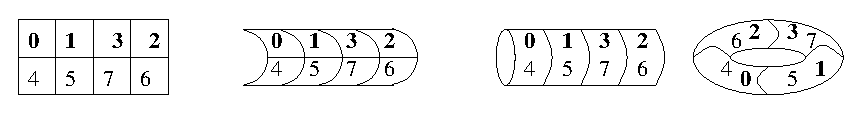
\includegraphics{./Fig3/Torus}}
\caption{The folding and stretching required to transform
a 3-variable Kmap onto the surface of a torus.  The shaded
numbers are on the back side of the surface.}
\label{fig:Torus}
\end{figure}

When a Kmap is solved correctly the resulting SOP expression
uses the minimum number of gates to realize the circuit 
in SOP form.  Such a minimal SOP expression is referred 
to as a \SOPmin \index{SOP!\SOPmin} expression.

\section{Karnaugh Maps}
Using a Kmap to determine a \SOPmin realization of a function
is a 4-step process.  This process is examined by 
determining the \SOPmin expression for the function 
$G(A,B,C)=\sum m(1,2,5,6)$.  Note, this expression is the
same function minimized earlier.  The first step is to draw
an empty Kmap using the input variables of the function $A,B,C$.
The second step is to place 1s in the Kmap for those inputs
for which the function is to equal 1.  Typically, the 0s of
the function are not put into the Kmap -- a blank space
in a Kmap occurs when the function is equal to 0.  The Kmap
below shows the Kmap for $G$.

$$ \begin{array} {c||c|c|c|c}
	A \bs BC & 00 & 01 & 11 & 10 \\ \hline \hline
	0        &    & 1  &    & 1  \\ \hline
	1        &    & 1  &    & 1  \\ 
\end{array} $$

The third step when using a Kmap is to identify pairs of
adjacent 1s in the Kmap, circle them, and then write down
the Boolean expression for the grouping.
In the example, the 1s in cell 1 and cell 5 are adjacent.  The
Boolean expression for this group is formed by applying
the minterm trick \label{trick!minterm}
(see page~\pageref{page:MinTrick}) to the variables which do 
not change.  Notice that $B=0$ for both cells and $C=1$ for 
both cells.  Since the $A$ variable changes, its value between
the two cells it will not be included in the product.  The 
Boolean expression for this grouping is $B'C$.  Circle 
this pair of cells indicating they have been covered.
Likewise, cell 2 and cell 6 can be combined resulting in the 
product term $BC'$.  The fourth step when using a Kmap 
is to OR together the products formed in the third step.  
This yields: $G(A,B,C) = B'C + BC'$.

To explore more fully how to solve Kmaps, consider the
following truth table which lists seven functions $F \ldots M$ 
each having three inputs.  The \SOPmin expression is derived 
for each of these functions, along the way 
illustrating many of the properties needed to solve Kmaps.

\begin{tabular}{c|c|c||c|c|c|c|c|c|c|c}
A & B & C & F & G & H & I & J & K & L & M  \\ \hline
0 & 0 & 0 & 0 & 0 & 0 & 1 & 1 & 1 & 1 & 0  \\ \hline
0 & 0 & 1 & 0 & 0 & 1 & 1 & 0 & 1 & 1 & 0  \\ \hline
0 & 1 & 0 & 0 & 1 & 0 & 0 & 1 & 1 & 0 & 0  \\ \hline
0 & 1 & 1 & 1 & 1 & 1 & 0 & 0 & 0 & 1 & 0  \\ \hline
1 & 0 & 0 & 1 & 0 & 0 & 0 & 1 & 0 & 1 & 0  \\ \hline
1 & 0 & 1 & 1 & 0 & 1 & 1 & 1 & 1 & 1 & 0  \\ \hline
1 & 1 & 0 & 0 & 0 & 0 & 0 & 0 & 1 & 0 & 0  \\ \hline
1 & 1 & 1 & 0 & 1 & 1 & 1 & 0 & 1 & 1 & 0  
\end{tabular}

\begin{description}
\item [$F= AB' + A'BC$]
\marginpar{ \tiny $$ \begin{array} {c||c|c|c|c}
        A \bs BC & 00 & 01 & 11 & 10 \\ \hline \hline
        0        &    &    & 1  &    \\ \hline
        1        & 1  & 1  &    &    \\
\end{array} $$ 
{\rm Kmap for }F }
The grouping of cell 4 and cell 5 yields the product term $AB'$.  
Cell 5 and cell 3 cannot be combined because they differ in two bits.
What is to do be done with the single cell 3?  Since this cell 
cannot be combined
with another cell, it is just a minterm by itself.  Sad perhaps, 
but perfectly legal.  Hence, $F(A,B,C) = AB' + A'BC$.

\item [$G=A'B + BC$]
\marginpar{ \tiny $$ \begin{array} {c||c|c|c|c}
        A \bs BC & 00 & 01 & 11 & 10 \\ \hline \hline
        0        &    &    & 1  & 1  \\ \hline
        1        &    &    & 1  &    \\
\end{array} $$ 
{\rm Kmap for }G }
The natural question arising from this Kmap is, ``Can 
cell 3 be reused in two different groups?"  The answer is ``Yes," and the reason
can be demonstrated by performing some Boolean Algebra on the canonical 
SOP expression for $G$.
$$\begin{array}{ll}
G(A,B,C) =	& A'BC' + A'BC + ABC = \\
		& A'BC' + A'BC + A'BC + ABC = \\
		& A'B(C' + C) + BC(A'+A) = \\
		& A'B(1) + BC(1) = \\
		& A'B + BC 
\end{array}$$
In the second line, the minterm $A'BC$ was duplicated using Law 3 of Boolean 
Algebra.  Note, this is the same minterm covered twice in the 
Kmap.  Consequently, if a cell of the Kmap is covered by three different
groupings then it would have to be replicated three times in the Boolean 
Algebra simplification.  

The grouping of cell 2 and cell 3 yields the product term $A'B$.  The 
grouping of cell 3 and cell 7 yield the product term $BC$.  
Consequently, $G(A,B,C) = A'B + BC$.  It is now possible to relate what 
happens in the symbolic expression when $(A,B,C) = (0,1,1)$ to the method
used to solve the Kmap.

\item [$H=C$] 
Grouping can be of size four.  This can be explained by performing Boolean 
Algebra on the canonical SOP expression for $H$.
\marginpar{ \tiny $$ \begin{array} {c||c|c|c|c}
        A \bs BC & 00 & 01 & 11 & 10 \\ \hline \hline
        0        &    & 1  & 1  &    \\ \hline
        1        &    & 1  & 1  &    \\
\end{array} $$
{\rm Kmap for }H }
$$\begin{array}{ll}
H(A,B,C) = 	& A'B'C + A'BC + AB'C + ABC = \\
		& (B+B')A'C + (B'+B)AC =  \\
		& A'C + AC = \\
		& (A'+A)C = \\
		& C 
\end{array}$$
In general, grouping can be of size $2^i \times 2^j$ for integer $i$ and $j$.
It is a common mistake of students to make a grouping of size 3x2 --  3 is not
a power of 2!

\item [$I=A'B'+AC$]
\marginpar{ \tiny $$ \begin{array} {c||c|c|c|c}
        A \bs BC & 00 & 01 & 11 & 10 \\ \hline \hline
        0        & 1  & 1  &    &    \\ \hline
        1        &    & 1  & 1  &    \\
\end{array} $$ 
{\rm Kmap for }I }
One does not have to form every possible grouping.  It is
a common error for students to include the term $B'C$ in the expression
for $I$.  The expression $B'C'$  does not cause the function to output
an incorrect value. Rather, this expression is not necessary for the
circuit to function properly.  Hence, including the expression $B'C'$ 
would make the circuit larger by one more AND gate than necessary.

\item [$J=A'C'+AB'$] 
\marginpar{ \tiny $$ \begin{array} {c||c|c|c|c}
        A \bs BC & 00 & 01 & 11 & 10 \\ \hline \hline
        0        & 1  &    &    & 1  \\ \hline
        1        & 1  & 1  &    &    \\
\end{array} $$ 
{\rm Kmap for }J }
Grouping can be made over the edge of the Kmap using the doughnut
\index{doughnut} (torus) property illustrated in Figure~\ref{fig:Torus}.
Notice, the minterms in the grouping on the upper row 
differ in the $B$ bit.

\item [$K=A'B'+AC+BC'$ or $K=A'C'+B'C+AC$]
\marginpar{ \tiny $$ \begin{array} {c||c|c|c|c}
        A \bs BC & 00 & 01 & 11 & 10 \\ \hline \hline
        0        & 1  & 1  &    & 1  \\ \hline
        1        &    & 1  & 1  & 1  \\
\end{array} $$ 
{\rm Kmap for }K }
A Kmap may have more than one correct solution.

\item [$L=B'+C$]
\marginpar{ \tiny
$$ \begin{array} {c||c|c|c|c}
        A \bs BC & 00 & 01 & 11 & 10 \\ \hline \hline
        0        & 1  & 1  & 1  &    \\ \hline
        1        & 1  & 1  & 1  &    \\
\end{array} $$ 
{\rm Kmap for }L }
Avoid the temptation to make a grouping of size $3 \times 2$.
Instead, make two groupings of size $2 \times 2$ which overlap 
in two cells.  Yes, overlapping big groupings is legal, too.

\item [$M=0$] \marginpar{ \tiny
$$ \begin{array} {c||c|c|c|c}
        A \bs BC & 00 & 01 & 11 & 10 \\ \hline \hline
        0        &    &    &    &    \\ \hline
        1        &    &    &    &    \\
\end{array} $$
{\rm Kmap for }M }
This trivial function can be confusing when first encountered.
Notice that regardless of the input, the output of the function 
is always 0.  Hence, $M=0$.
\end{description}

The process of ``solving" a Kmap correctly leads to a minimal 2-level 
SOP expression (abbreviated \SOPmin).  SOP expressions are composed
of two main levels of gates. A set of AND gates (level 1) leading 
into an OR gate (level 2).  The NOT gates are ignored because they are 
both small and fast compared to AND and OR gates.  The term ``minimal"
refers to the fact that the realization of the function requires 
the fewest possible gates among any 2-level SOP realizations.  

In order to understand how to most efficiently solve a Kmap, some
notation needs to be defined.
An {\it implicant} \index{Implicant} is a legal grouping of 1s in 
a Kmap.  An implicant which is not contained in any other implicant 
is called a {\it prime implicant} \index{Implicant!Prime}.  An 
{\it essential prime implicant} \index{Implicant!Essential Prime} 
is a prime implicant which covers a minterm not covered by any other 
prime implicant. For example, $ABC$ is an implicant in the function 
$L(A,B,C)$, but it is not a prime implicant because it is contained in 
the essential prime implicant $C$.

When solving a Kmap, look for essential prime implicants and 
remove them from consideration.  Removing the 1s from consideration does not
mean removing the 1s from the problem.  If needed, the 1s in an essential
prime implicant can be used to form other groupings.
After the essential prime implicants 
have been removed, look for {\it secondary essential prime implicants}, 
the essential largest groupings covering the remaining 1s.
 This identification of essential
prime implicants goes on until either all the 1s are covered or 
a situation like the $K$ function results.  The $K$ function has no 
essential prime implicants.  At this point, resort to intuition 
(or brute force search) to minimize the number of groupings
to cover the remaining 1s in the Kmap.  Kmaps can be used to 
minimize functions in a variety of ways.  One such use is discussed below.

Determine the \SOPmin expression for $F(A,B,C) = B'C' + BC' + ABC$.  The
\label{page:SymbToSymb} term \SOPmin implies that a Kmap is 
required to solve the problem. In this case, figure out a way 
determine which region of the Kmap is described by each product term.  
For example, the product term $B'C'$ is equal to 1 when $(B,C) = (0,0)$.
Thus, 1s are placed in cell 0 and cell 4 of the Kmap. The product term $BC'$
results in 1s being placed in cell 2 and cell 6.  The product term $ABC$
requires a 1 to be placed in cell 7.  The resulting Kmap is shown in the 
margin.
\marginpar{\tiny
$$ \begin{array} {c||c|c|c|c}
	A \bs BC & 00 & 01 & 11 & 10 \\ \hline \hline
	0        & 1  &    &    & 1  \\ \hline
	1        & 1  &    & 1  & 1  \\ 
\end{array} $$
}
This Kmap can now be solved to determine the \SOPmin expression;
$F(A,B,C) = C'+AB$.  Incidentally, the grouping of cells 0, 2, 4, 6
in the Kmap above is affectionately referred to as a 
\index{doughnut!Texas} {\it Texas doughnut} because it has a big 2x2 
grouping straddling the ends of the Kmap.


\section{4-Variable Kmaps}
The Kmap method can be adapted to work with functions of more than three
variables.  These larger Kmaps must be constructed so that adjacent 
cells differ by a single bit in order for the simplification trick 
to work.  For example, a 4-variable Kmap is shown below with the 
decimal equivalent of the binary inputs shown in each cell.

$$ \begin{array} {c||c|c|c|c}
	AB \bs CD & 00 & 01 & 11 & 10 \\ \hline \hline
	00        & 0  & 1  & 3  & 2  \\ \hline
	01        & 4  & 5  & 7  & 6  \\ \hline
	11        & 12 & 13 & 15 & 14 \\ \hline
	10        & 8  & 9  & 11 & 10 \\ 
\end{array} $$

It is easy to verify that adjacent cells differ by a single bit.
In addition, notice that adjacencies run across the top/bottom 
and left/right margins of the Kmap.  In order to better 
understand this new structure, determine the \SOPmin
expressions for the following functions. 

\begin{itemize}
\item $F(A,B,C,D) = \sum m(0,1,4,5,8,9)$
\item $G(A,B,C,D) = \sum m(0,5,7,10,11,14,15)$
\item $H(A,B,C,D) = \sum m(0,2,3,5,6,7,8,10,11,14,15)$
\end{itemize}

\begin{description}
\item [$F=A'C'+B'C'$]  
\marginpar{ \tiny $$ \begin{array} {c||c|c|c|c}
       AB \bs CD & 00 & 01 & 11 & 10 \\ \hline \hline
       00        &  1 &  1 &    &    \\ \hline
       01        &  1 &  1 &    &    \\ \hline
       11        &    &    &    &    \\ \hline
       10        &  1 &  1 &    &    \\
\end{array} $$ 
{\rm Kmap for} F}
Resist the temptation to make a grouping of size $3 \times 2$;
3 is not a power of 2.  Notice, one of the $2 \times 2$
groupings, $B'C'$ spans the edge of the Kmap (Texas doughnut style).


\item [$G=A'B'C'D'+A'BD+AC$] 
\marginpar{ \tiny $$ \begin{array} {c||c|c|c|c}
       AB \bs CD & 00 & 01 & 11 & 10 \\ \hline \hline
       00        &  1 &    &    &    \\ \hline
       01        &    &  1 &  1 &    \\ \hline
       11        &    &    &  1 & 1  \\ \hline
       10        &    &    &  1 & 1  \\
\end{array} $$ 
{\rm Kmap for} G}
This example demonstrates an interesting point: The size of the 
grouping determines the number of variables in the \SOPmin expression.
For example, the grouping for covering one cell, $A'B'C'D'$, has four
variables, the grouping covering two cells, $A'BD$, has three variables 
and the grouping covering four cells, $AC$, has two variables.  The 
larger the grouping, the fewer variables that are required to describe
the grouping, and consequently requires a smaller AND gate.

\item [$H=B'D'+A'BD+C$] 
\marginpar{ \tiny $$ \begin{array} {c||c|c|c|c}
       AB \bs CD & 00 & 01 & 11 & 10 \\ \hline \hline
       00        &  1 &    &  1 &  1 \\ \hline
       01        &    &  1 &  1 &  1 \\ \hline
       11        &    &    &  1 &  1 \\ \hline
       10        &  1 &    &  1 &  1 \\
\end{array} $$ 
{\rm Kmap for} H}
This solution is notable because it contains the 
{\it HyperDoughnut} \index{Doughnut!Hyper} grouping -- the cells
0,2,8,10 forming the product $B'D'$.  The only other notable 
feature in this Kmap is the large grouping of size 8, $C$.
\end{description}


\section{5-Variable Kmaps}
A 5-variable Kmap is a rearrangement of the rows of a 5-variable
truth table such that adjacent cells of the Kmap differ by a single
input bit.  This rearrangement is accomplished by floating two, 4-variable 
Kmaps one above the other.  A cell in a 5-variable Kmap can be combined with
the cell to its left, right, below, above, up or down!  That is, the three
perpendicular directions along which adjacencies lie must be checked.

Determine the \SOPmin expression for \\
$F(A,B,C,D,E) = \sum m(0,1,2,5,7,8,10,15,16,18,23,24,26,28,29,31)$.
Each of the 4-variable Kmaps is labeled with one of the two possible
values of $A$, 0, or 1.  The decimal values of the inputs can be formed
by converting the binary input $ABCDE$ for each cell into decimal.  The 
4-variable Kmap with $A=0$ is labeled just like an ordinary 4-variable 
Kmap.  The 4-variable Kmap with $A=1$ is labeled in the same order as a 
regular 4-variable Kmap, except the numbering starts at 16 because the MSB
is 1.

$$\begin{array}{cc} 
\begin{array} {c||c|c|c|c}
	BC \bs DE & 00 & 01 & 11 & 10 \\ \hline \hline
	00        & 1  & 1  &    & 1  \\ \hline
	01        &    & 1  & 1  &    \\ \hline
	11        &    &    & 1  &    \\ \hline
	10        & 1  &    &    & 1  \\ 
\end{array}
&
\begin{array} {c||c|c|c|c}
	BC \bs DE & 00 & 01 & 11 & 10 \\ \hline \hline
	00        & 1  &    &    & 1  \\ \hline
	01        &    &    & 1  &    \\ \hline
	11        & 1  & 1  & 1  &    \\ \hline
	10        & 1  &    &    & 1  \\ 
\end{array} \\
A=0 & A=1 \\
\end{array}
$$

This Kmap is notable because it contains the granddaddy of all the
border jumping groupings, the \index{Doughnut!Ultra} {\it ultra-doughnut}.  
This grouping occupies the eight corners of the 5-variable Kmap.  
A grouping of size four jumps between the two Kmaps.  
Other than this aspect, the solution is fairly straightforward.
$F(A,B,C,D,E)=C'E'+A'B'D'E+CDE+ABCD'$

To conclude the Kmap concept, a few trends 
should be noted.  First, there is a relationship between the
number of variables in a Kmap and the number of neighbors.
\\ \\
\begin{tabular}{l|l}
Variables & Neighbors	\\ \hline
3	  &  3		\\ \hline
4	  &  4		\\ \hline
5	  &  5		\\ 
\end{tabular}
\\ \\
The relationship is linear, that is a cell in a Kmap with 
$N$ variables should have $N$ neighbors.   By considering
the simplification trick, this relationship should make sense. Two cells
are adjacent if their binary representations differ by a single
bit.  An $N$-bit number has $N$ positions where a single bit
could be changed, thus it has $N$ neighbors in the Kmap.  

Also there is a relationship between the number of 1s in a 
grouping and the number of variables appearing in the grouping's
product term.  For example, in the $G(A,B,C,D)$ function
above, the grouping of a single minterm was described by the
product term $A'B'C'D'$ containing four variables.  The largest
grouping of four  minterms was described by the product term
$AC$ containing two variables.  The following table describes 
this relationship for a 5-variable function.
\\ \\
\begin{tabular}{l|l}
Number of 1's	& Variables  \\ \hline
32		&	0	\\ \hline
16		&	1	\\ \hline
8		&	2	\\ \hline
4		&	3	\\ \hline
2		&	4	\\ \hline
1		&	5	\\ 
\end{tabular}
\\ \\
This table demonstrates why making the groupings as large
as possible is desirable, large groupings have smaller AND gates.

\section{Multiple Output Circuits}
In the previous chapter, digital systems with more than one output 
were considered.  Multiple output functions are realized by
realizing each output independently of the others. For example, 
consider a digital system with three inputs $A,B,C$ and two outputs 
$F(A,B,C)$ and $G(A,B,C)$ shown in the truth table below:

\marginpar{ \tiny
$$ \begin{array} {c||c|c|c|c}
        A \bs BC & 00 & 01 & 11 & 10 \\ \hline \hline
        0        &    &    & 1  &    \\ \hline
        1        & 1  & 1  &    &    \\
\end{array} $$
$F(A,B,C) = AB' + A'BC$

$$ \begin{array} {c||c|c|c|c}
        A \bs BC & 00 & 01 & 11 & 10 \\ \hline \hline
        0        &    &    & 1  & 1  \\ \hline
        1        &    &    & 1  &    \\
\end{array} $$
$G(A,B,C) = BC + A'BC'$
}

$$\begin{array}{c|c|c||c|c}
A & B & C & F & G \\ \hline
0 & 0 & 0 & 0 & 0 \\ \hline
0 & 0 & 1 & 0 & 0 \\ \hline
0 & 1 & 0 & 0 & 1 \\ \hline
0 & 1 & 1 & 1 & 1 \\ \hline
1 & 0 & 0 & 1 & 0 \\ \hline
1 & 0 & 1 & 1 & 0 \\ \hline
1 & 1 & 0 & 0 & 0 \\ \hline
1 & 1 & 1 & 0 & 1 \\
\end{array}$$

If the functions are solved independently of one another,
$F(A,B,C)=AB'+A'BC$ and $G(A,B,C) = BC + A'BC'$.  The only
connection the two circuits have to each other is their inputs, both
share the same $(A,B,C)$.  Thus, when $(A,B,C) = (1,0,1)$ 
$F=1$ and $G=0$ just as expected according to
the truth table.  The circuit diagram of the $F$ and $G$ 
functions is shown in Figure~\ref{fig:MultiOut}.

\begin{figure}[ht]
\center{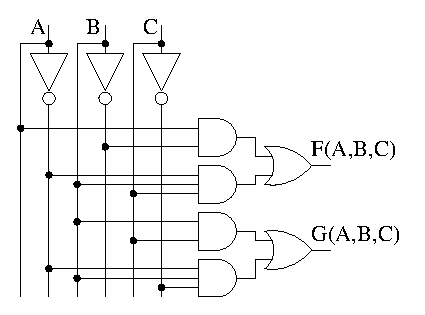
\includegraphics{./Fig3/MultiOut}}
\caption{Two functions, $F$ and $G$, which share inputs.}
\label{fig:MultiOut}
\end{figure}

When more than one function shares the same input, 
often product terms are shared.  A shared product term is an AND
gate that can be used in the realization of more than one 
function.  For example, consider the two functions 
$H(A,B,C) = \sum m(1,4,5,6)$ and $I(A,B,C) = \sum m(1,2,3,5)$.
\label{page:DualFnc}
\marginpar{ \tiny
$$ \begin{array} {c||c|c|c|c}
        A \bs BC & 00 & 01 & 11 & 10 \\ \hline \hline
        0        &    & 1  &    &    \\ \hline
        1        & 1  & 1  &    & 1  \\
\end{array} $$
$H(A,B,C) = \sum m(1,4,5,6) = B'C + AC'$

$$ \begin{array} {c||c|c|c|c}
        A \bs BC & 00 & 01 & 11 & 10 \\ \hline \hline
        0        &    & 1  & 1  & 1  \\ \hline
        1        &    & 1  &    &    \\
\end{array} $$
$I(A,B,C) = \sum m(1,2,3,5) = B'C + A'B$ 
}

The Kmaps and the solutions for these two functions are shown in 
the margins.  Notice that the grouping $B'C$ appears in both
\SOPmin expressions.  This AND gate need appear only once in the
circuit diagram because its output can be directed to both OR gates 
which form the outputs for $H$ and $I$.  The circuit diagram for 
these two functions is shown in Figure~\ref{fig:Share}.

\begin{figure}[ht]
\center{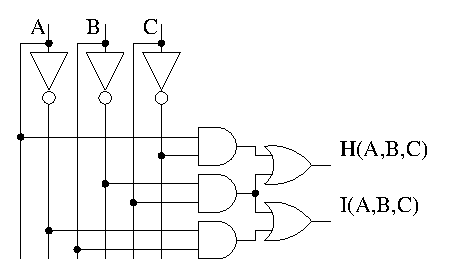
\includegraphics{./Fig3/Share}}
\caption{Two functions which share the product term $B'C$.}
\label{fig:Share}
\end{figure}

\section{``Don't Cares"}
There are situations when engineers ``don't care" what the output of a
digital system is for certain inputs.  This situation often happens when 
a particular input will never occur.  For example, consider the 
a digital system which classifies its inputs as either even or
odd.  It has four bits of input $a_3 a_2 a_1 a_0$, and one bit 
of output, $F$.  The 4-bit input represents a decimal number, 
$0 \le A \le 9$, the inputs $10 \le A \le 15$ should never be
applied.  The output equals 1 when $A$ is even ( 0 is considered 
an even number) and outputs 0 when $A$ is odd.

As a first attempt to solve this problem, ignore the inputs 
corresponding to $10 \le A \le 15$ and leave the 
corresponding outputs blank.  The outputs are to be defined
for inputs $0 \le A \le 9$. The resulting Kmap and its solution
is shown in the margins.

\marginpar{ \tiny
$$ \begin{array} {c||c|c|c|c}
a_3 a_2 \bs a_1 a_0 & 00 & 01 & 11 & 10 \\ \hline \hline
	00          & 1  &    &    & 1  \\ \hline
	01          & 1  &    &    & 1  \\ \hline
	11          &    &    &    &    \\ \hline
	10          & 1  &    &    &    \\ 
\end{array} $$
$F(a_3,a_2,a_1,a_0)=a_3'a_0'+ a_2'a_1'a_0'$
}

The solution shown in the margin will certainly work correctly,
since the outputs are correctly defined for the legitimate inputs.
However, the realization could have been made more efficient
if the fact that the inputs $10 \le A \le 15$ will never be applied 
had been taken into consideration. Then, it does not matter what the 
circuit outputs when $10 \le A \le 15$.  Notice, that in the first 
solution, implicitly
the illegal inputs were treated as odd numbers; the circuit would
output a 0 for $10 \le A \le 15$. Since these are illegal inputs,
they are assigned any convenient value with an eye on making 
the final realization as
efficient as possible.  To denote this freedom in assigning the
output of the function either value, an ``X" is placed in any 
cell of the Kmap where the output doesn't matter.  These
Xs are referred to as ``don't cares".

The utility of ``don't cares" lies in the fact that they can be 
used to make groupings larger and consequently the realization
of the function more efficient.  If an X can be used to make a 
grouping larger, then it should be included in that grouping.
Including ``don't cares" in a group will cause the circuit to
output 1 for the input corresponding to the ``don't care".  
If, on the other hand,
an X cannot be used in any grouping, then leave it uncovered.
The circuit will output a 0 for the uncovered ``don't care".

To better understand how ``don't cares" are used, they are included
into the even/odd function for inputs $10 \le A \le 15$ and the
resulting Kmap shown in the margin is solved.

\marginpar{ \tiny
$$ \begin{array} {c||c|c|c|c}
a_3 a_2 \bs a_1 a_0 & 00 & 01 & 11 & 10 \\ \hline \hline
	00          & 1  &    &    & 1  \\ \hline
	01          & 1  &    &    & 1  \\ \hline
	11          & X  & X  & X  & X  \\ \hline
	10          & 1  &    & X  & X  \\ 
\end{array} $$
$F(a_3,a_2,2_1,a_0)=a_0'$
}

By using the ``don't cares" in cells 10, 12, and 14, a grouping of
size eight is formed.  This grouping reduces the cost of the solution
to a single inverter.

``Don't cares" are included in the abbreviated canonical SOP form by 
writing a ``$d$" followed by a list of inputs for which the output is
unimportant.  For example, the even/odd function is described 
as $F(A,B,C,D) = \sum m(0,2,4,6,8) + \sum d(10,11,12,13,14,15)$.

``Don't cares" can be used on the input variables of a truth table 
in order to compress the size of the truth table.  Two rows can
be combined when their outputs are the same and their inputs are
adjacent (in the Kmap sense) to one another.  A single ``don't care"
on an input of a row of a truth table generates two rows; one 
with the ``don't care" set to 1 and another with the ``don't care"
set to 0.  For example, the following two truth tables describe 
the same function.

\begin{tabular}{ll}
\begin{tabular}{c|c|c||c}
A & B & C & F(A,B) \\ \hline
x & 0 & x & 0 \\ \hline
x & 1 & 0 & 1 \\ \hline
0 & 1 & 1 & 0 \\ \hline
1 & 1 & 1 & 1 \\ 
\end{tabular} 

&

\begin{tabular}{c|c|c||c}
A & B & C & F(A,B) \\ \hline
0 & 0 & 0 & 0 \\ \hline
0 & 0 & 1 & 0 \\ \hline
0 & 1 & 0 & 1 \\ \hline
0 & 1 & 1 & 0 \\ \hline
1 & 0 & 0 & 0 \\ \hline
1 & 0 & 1 & 0 \\ \hline
1 & 1 & 0 & 1 \\ \hline
1 & 1 & 1 & 1 \\ 

\end{tabular}  \\
Compressed Truth Table & Full Truth Table \\
\end{tabular}

The row $(x,1,0)$ generates two rows in the full truth 
table, $(0,1,0)$ and $(1,1,0)$.  
The row $(A,B,C)=(x,0,x)$ has two ``don't cares".  Since
the values of these ``don't cares" can be selected
independent of one another, this row generates four
rows in the full truth table, $(0,0,0)$, $(0,0,1)$,
$(1,0,0)$, and $(1,0,1)$. In general, a row with $N$ 
``don't cares" generates $2^N$ rows in the full 
truth table.  The motivation for using ``don't cares"
will become more clear in later chapters when digital 
systems with six or more inputs are encountered.

\section{Minimizing to POS}
So far, the chapter has focused on finding efficient 
\SOPmin realizations of circuits.  However, 
Section~\ref{sec:TTtoSymb} provided a function whose POS 
realization was less costly than the SOP realization.
It is not difficult to imagine functions 
for which the \POSmin realization is less costly than 
the \SOPmin realization. In order to derive the 
\POSmin realization of a function $F$, the function
is transformed -- put into a Kmap, a \SOPmin realization
found, and then the \SOPmin realization transformed 
into a \POSmin realization for $F$.  In order for this 
process to work, the two transformations of the function
will have to ``undo" one another so they have no net 
effect on the function.

In order to cover all possibilities, the transform from any of 
the starting forms into one of the ending forms is investigated.

\begin{tabular}{lcr}
$\sum m$   &                    & 	  \\ 
$\prod M$  & $\longrightarrow$  & \SOPmin  \\ 
SOP        &                    & \POSmin \\ 
POS        &                    &     	  \\ \hline
Starting   &                    &  Ending \\ 
Form       &                    &  Form   \\ 
\end{tabular}
\\ \\
Eight potential transforms need to be
explored.  For each transformation, a plan is developed;
a series of steps.  The following five facts 
become the steps in all these plans.

\begin{description}
\item [1] Negating a Kmap for $F$ negates $F$.  If all the 
bits in a Kmap for a function $F$ are flipped, then it is
the same as negating the output of $F$.

\item [2] Negating a SOP expression for $F$ yields a POS 
\label{page:second} expression for $F'$.  This statement is 
based on Law 9 and Law 9D of Boolean Algebra.  Law 9 states that 
$(x+y)' = x'y'$.  Law 9D states that $(xy)' = x'+y'$.
The transformation from SOP to POS is illustrated
in the following example.

\begin{tabular}[ht]{ll}
$F  = A'B'C' + A'BC + AB' + C$      & negate F \\
$F' = (A'B'C' + A'BC + AB' + C)'$   & Law 9 \\
$F' = (A'B'C')'(A'BC)'(AB')'(C)'$   & Law 9D \\
$F' = (A+B+C)(A+B'+C')(A'+B)(C')$  \\
\end{tabular}

The shortcut typically used to determine the POS expression
is to replace all ANDs and ORs and negate each variable. 

\item [3] Negating a POS expression for $F$ yields a SOP 
expression for $F'$.  The proof of this statement is
derived by examining the previous algebraic example from
bottom to top.

\item [4] $\sum m(list) = \prod M(list')$.  $list'$ 
denotes the decimal numbers not in $list$.  Since $list$ 
describes those inputs for which the function equals 1, 
$list'$ describes those inputs for which the function 
equals 0. 

\item [5] $F'' = F$.  This expression is just Law 4 of Boolean Algebra.
\end{description}

The plans used to transform between forms consist 
of a sequence of steps.  At each step, the function 
(or its complement) is represented in one
of its various forms (Kmap, SOP, $\sum m$, etc..). 
Step 1 always describes the given form of the function.  
Likewise, the last step always describes the desired form
of the function.  The action between the steps is implicit
from the beginning and ending forms.  

To better understand how a plan is put together and how the
transformations are performed, consider a plan for the
transformation of a $\sum m$ expression into a \SOPmin realization.

%% \subsection{$\sum m(\ldots)$ to \SOPmin}
\begin{tabular}{|c|c|c|c|}\hline
Step	  & 1  & 2  & 3   \\ \hline
Function  & F  & F  & F \\ \hline
Form	  & $\sum m(\ldots)$ & Kmap & \SOPmin \\ \hline
\end{tabular}
\\ \\
The plan consists of three steps.  The function in all three steps is $F$.   
In Step 1, the function $F$ is written in the $\sum m(\ldots)$
notation.  In the second step, the function is placed into
a Kmap using the process outlined in this chapter. In the 
third step, the \SOPmin expression is derived from the Kmap.
Another familiar transform is handled next.

%% \subsection{SOP to \SOPmin}
\begin{tabular}{|c|c|c|c|}\hline
Step	  & 1  & 2  & 3   \\ \hline
Function  & F  & F  & F \\ \hline
Form	  & SOP & Kmap & \SOPmin \\ \hline
\end{tabular}
\\ \\
The only difference in this transformation is the beginning 
form.  The discussion on page~\pageref{page:SymbToSymb} 
illustrates how to put a SOP form into a Kmap.  Once in a 
Kmap, the remaining steps should be clear.  The next 
transformation is slightly trickier.

%% \subsection{$\sum m(\ldots)$ to \POSmin}
\begin{tabular}{|c|c|c|c|c|c|}\hline
Step	  & 1  & 2  & 3  & 4  & 5   \\ \hline
Function  & F  & F  & F' & F' & F''=F \\ \hline
Form	  & $\sum m(\ldots)$ & Kmap & Kmap' & \SOPmin & \POSmin \\ \hline
\end{tabular}
\\ \\
In Steps 1 and 2 of the plan, the function, $F$, is placed into a Kmap.
In Step 3, the Kmap is inverted (all the 1s replaced with 0s and 
0s replaced with 1s).  With this inversion, the 
\SOPmin expression for $F'$ determined from the Kmap 
can be negated, yielding a \POSmin expression for $F''=F$.  

An example shows how this plan is put into practice.
Determine the \POSmin expression for $F(A,B,C) = \sum m(3,4,5)$.

\begin{description}

\item [Step 1] $F(A,B,C) = \sum m(3,4,5)$.

\item [Step 2] The Kmap for $F$ is shown in the margin.
\marginpar{ \tiny 
$$ \begin{array} {c||c|c|c|c}
        A \bs BC & 00 & 01 & 11 & 10 \\ \hline \hline
        0        &    &    & 1  &    \\ \hline
        1        & 1  & 1  &    &    \\ 
\end{array} $$
{\rm Kmap for }F }


\item [Step 3] The Kmap for $F'$ is shown in the margin.
\marginpar{ \tiny 
$$ \begin{array} {c||c|c|c|c}
        A \bs BC & 00 & 01 & 11 & 10 \\ \hline \hline
        0        & 1  & 1  &    & 1  \\ \hline
        1        &    &    & 1  & 1  \\ 
\end{array} $$
{\rm Kmap for }F' }


\item [Step 4] $F'(A,B,C)= A'B'+AB+BC'$; note, the
		two potential solutions.
\item [Step 5] $F(A,B,C)= (A+B)(A'+B')(B'+C)$ 
		
\end{description}

The \POSmin expression for $F$ can be checked to generate
the correct outputs, by plugging in values for $A,B,C$.
The \SOPmin expression
for $F$ can be determined from the Kmap in Step 2 as
$F(A,B,C)=AB'+A'BC$.  This fact demonstrates, in general,
the \SOPmin and \POSmin realizations have different costs.

%% \subsection{SOP to \POSmin} \index{SOP!to \POSmin}
\begin{tabular}{|c|c|c|c|c|c|}\hline
Step	  & 1  & 2  & 3  & 4  & 5  \\ \hline
Function  & F  & F  & F'  & F' &  F''=F \\ \hline
Form	  & SOP & Kmap & Kmap' & \SOPmin & \POSmin \\ \hline
\end{tabular}
\\ \\
This transformation is the same as the $\sum m(\ldots)$ to \POSmin
transformation from Step 2 onward.

%% \subsection{$\prod M(\ldots)$ to \SOPmin}
\begin{tabular}{|c|c|c|c|c|}\hline
Step	  & 1  & 2  & 3  & 4     \\ \hline
Function  & F  & F  & F  & F  \\ \hline
Form	  & $\prod M(\ldots)$ & $\sum m(\ldots)$ & Kmap & \SOPmin \\ \hline
\end{tabular}
\\ \\
This transformation utilizes the fourth helpful fact.  The swapping of the
list of 0s for a list of 1s.  From Step 2 onwards this transformation 
should look familiar.

%% \subsection{$\prod M(\ldots)$ to \POSmin}
\begin{tabular}{|c|c|c|c|c|c|c|}\hline
Step	  & 1  & 2  & 3  & 4  & 5  & 6\\ \hline
Function  & F  & F  & F  & F' & F' & F''=F \\ \hline
Form	  & $\prod M(\ldots)$ & $\sum m(\ldots)$ & Kmap & Kmap' & \SOPmin & \POSmin \\ \hline
\end{tabular}
\\ \\
In Step 2, the list of maxterms, given in Step 1, is transformed into a list
of minterms.  The Kmap is negated in Step 4 so that the \SOPmin description
of $F'$ can be negated, yielding a \POSmin expression for $F$.

%% \subsection{POS to \SOPmin} \index{POS!to \SOPmin}
\begin{tabular}{|c|c|c|c|c|c|}\hline
Step	  & 1  & 2  & 3  & 4  & 5  \\ \hline
Function  & F  & F'  & F'  & F''=F &  F \\ \hline
Form	  & POS & SOP & Kmap & Kmap' & \SOPmin \\ \hline
\end{tabular}
\\ \\
This is an interesting transformation because $F$ must be negated
before being placed into a Kmap.  Since $F'$ is in the Kmap, the
Kmap must be negated so that the solution to the Kmap
yields a \SOPmin expression for $F$.

%% \subsection{POS to \POSmin}
\begin{tabular}{|c|c|c|c|c|c|}\hline
Step	  & 1  & 2  & 3  & 4  & 5  \\ \hline
Function  & F  & F'  & F'  & F' &  F''=F \\ \hline
Form	  & POS & SOP & Kmap & \SOPmin & \POSmin \\ \hline
\end{tabular}
\\ \\
In Step 2 the POS expression, given in Step 1, is negated 
so that it can be placed into a Kmap.  But this time the Kmap is not
negated because the \SOPmin expression $F'$ is negated, yielding 
a \POSmin expression for $F$.

\section{Espresso}
The Kmap minimization method can be applied to problems with up to
eight variables.  Beyond eight variable, the process becomes too tedious and error-prone to
be practical.  Functions with 20 variables are not uncommon, but 
would require a truth table containing over a million rows!  An 
algorithmic approach is needed to handle such large instances.  
Espresso is a 2-level logic minimization tool, that while not 
guaranteed to find a minimal solution, does a good job on most 
functions.  Since Espresso was written before the days 
of visual interfaces, it is a small program, run from a command line interface.  
(A command line interface
is a text interface to the programs and operating services
available to the user of a computer.) The operating system prompts
the user by displaying a ``$>$" character in a window. The user
then types in the name of the program or service they want to 
access.  Typing ``espresso" at the command
line prompt invokes the Espresso program.

Espresso is simple to use, just create the truth table for 
a function in a text editor, then run Espresso on the file.
The input file for Espresso contains:
\begin{enumerate}
\item {\bf Comments.}  Comments are always preceded with 
the \# symbol.  If a comment is encountered, Espresso 
ignores the rest of the line.

\item {\bf The number of inputs.}
The number of inputs is 
described by the statement \verb+.i+ followed by a 
number describing the number of inputs to the function. 
The \verb+.i+  must be included in an Espresso file.

\item {\bf The number of outputs.}
The number of outputs 
is described by the statement \verb+.o+ followed by 
a number describing the number of outputs from the function. 
The \verb+.o+ must be included in an Espresso file.

\item {\bf The labels for the inputs.}
The labels for the inputs are described by the statement \verb+.ilb+ 
followed by a list of names of the inputs separated by spaces.  
The \verb+.ilb+ does not have to be included in an
Espresso file.  If not included, then Espresso assigns its
own names to the inputs.

\item {\bf The labels for the output(s).}
The labels for the outputs are described by the statement \verb+.ob+ 
followed by a list of names of the outputs separated by spaces.
The \verb+.ob+ does not have to be included in an
Espresso file.  If not included, then Espresso assigns its
own names to the outputs.

\item {\bf The truth table.}
The truth table is organized with the input bits on the left and the 
output(s) bit(s) on the right.  ``Don't cares" in the inputs or outputs
are denoted with a minus sign -.  The order of the rows in the truth
table is unimportant.  

\end{enumerate}

The following is an example Espresso input file for the function
$F(a,b,c) = \sum m(1,3,6,7)$.  

\begin{verbatim}
        # File: simple.txt
        # Name: <your name>
        #       <course name>
        # Date: <semester>
        # Desc: F(a,b,c) = sum m(1,3,6,7)
        .i 3
        .o 1
        .ilb a b c
        .ob F
        
        000 0
        001 1
        010 0
        011 1
        100 0
        101 0
        110 1
        111 1
\end{verbatim}

This file must be created in text format -- do not create this document
in a ``word processor" such as MS Word or WordPerfect.  NotePad, Edit, 
emacs, or vi are preferable choices for creating this file.  Save 
the example Espresso file as \verb+simple.txt+.  The command
line 

Running
Espresso on the example file produces the following output.

\begin{verbatim}
        > espresso simple.txt
        # File:	simple.txt
        # Name: <your name>
        #       <course name>
        # Date: <semester>
        # Desc:	F(a,b,c) = minterms (1,3,6,7)
        .i 3
        .o 1
        .ilb a b c
        .ob F
        .p 2
        11-     1
        0-1     1
        .e
\end{verbatim}

Espresso echoes back comments, the number of inputs, outputs, 
and labels defined in the input file,  and identifies the number of product
terms used in the realization.  In the example, the 
\verb+.p 2 + statement means that the solution found by Espresso 
required two product terms.  The two lines after the \verb+.p 2 + 
statement describe the realization in a programmable logic 
array (PLA) format.  In the PLA format, each row represents a 
product term.  The left three columns of each row represent the 
state of the inputs variable in the product term.  The variables 
are in the same order as they were defined in the truth table.
The state of a variable can be ``1", ``0", or ``-".
\begin{itemize}
\item 1 means, include the variable in the product.
\item 0 means, include the negated variable in the product.
\item - means, exclude the variable from the product.
\end{itemize}

Thus, the row ``11-" represents the product term $AB$ and the row ``0-1"
represents the product term $A'C$.  The column of 1s to the right 
of these bits describes which product terms to use in the realization
of the function.  A 1 means to include the product term in the 
function, 0 means exclude the product term from the function -- 
and is seen only for two or more outputs.

Putting both of Espresso's product terms together yields the
optimal solution $F=A'C+AB$.  The Kmap for this function and
its \SOPmin solution is shown in the margin.

\marginpar{ \tiny 
$$ \begin{array} {c||c|c|c|c}
        A \bs BC & 00 & 01 & 11 & 10 \\ \hline \hline
        0        &    & 1  & 1  &    \\ \hline
        1        &    &    & 1  & 1  \\ 
\end{array}$$ 
$F(A,B,C) = A'C + AB$}


Command line parameters can be included to specify options, 
 changing the behavior of Espresso.
All options consist of a minus sign, a letter, and a command, 
placed between ``espresso" and the name of the input file. As an 
example the \verb+-o eqntott+ option will force Espresso to generate a
symbolic output instead of the default PLA output.

\begin{verbatim}
        > espresso -o eqntott simple.txt
        #comments
        F = (a&b) | (!a&c);
\end{verbatim}

The entire set of options is listed by typing 
\verb+espresso -help+ at the command prompt. The \verb+-epos+ option
inverts the truth table, yielding a SOP solution for
$F'$.  The POS solution is generated by inverting Espresso's
output using the second helpful fact on page~\pageref{page:second}.
This option allows a digital designer to quickly compare the
cost of a SOP and POS realization.

Generated output can be saved by Espresso by redirecting standard
output to a file.  This option is indicated by putting a ``greater than" symbol after a
command, followed by the name of the output file.
Think of the ``greater than" symbol as a funnel, taking 
the streaming output of the Espresso program and funneling it into
the output file.  For example, the output of the previous Espresso example can
be saved into a file called \verb+simple.out+ using the following command.

\begin{verbatim}
        a:\> espresso -o eqntott simple.txt > simple.out
\end{verbatim}

Espresso can solve design problems involving multiple outputs. The
following Espresso file describes the example on 
page~\pageref{page:DualFnc}, where 
$F(A,B,C) = \sum m(1,4,5,6)$ and $G(A,B,C) = \sum m(1,2,3,5)$.  

\begin{verbatim}
        # File: harder.txt
        # Name: <your name>
        #       <course name>
        # Date: Fall 2020
        # Desc: F(a,b,c) = minterms(1,4,5,6)
        #       G(a,b,c) = minterms(1,2,3,5)
        
        .i 3
        .o 2
        .ilb a b c
        .ob F G
        
        
        000 00
        001 11
        010 01
        011 01
        100 10
        101 11
        110 10
        111 00
        .e
\end{verbatim}

The output from Espresso is:
\begin{verbatim}
        a:\> espresso harder.txt 
        # Comments
        .i 3
        .o 2
        .ilb a b c
        .ob F G
        .p 3
        1-0 10
        01- 01
        -01 11
        .e
\end{verbatim}

Espresso used three product terms to realize the functions $AC'$, $A'B$,
and $B'C$.  The two columns to the right of the product terms 
describe which product terms are used to realize each outputs. 
Symbolically, the solution found by Espresso is:
\begin{itemize}
\item $F(A,B,C)= AC' + B'C$
\item $G(A,B,C)= A'B + B'C $
\end{itemize}

The circuit diagram of the realization for the three functions is
shown in Figure~\ref{fig:Share}.  Notice, the connections --
denoted by dots -- between the inputs and the AND gates has a pattern
which is similar to the PLA description of the product terms by
Espresso.  Likewise, the pattern formed by the connections of the AND
gates and OR gates is similar to the rightmost three columns of the
Espresso output.  This similarity is no accident; the designers of Espresso 
used a generalized layout of the of the circuit diagram in 
Figure~\ref{fig:Share} as a template to describe the output.

\section{Minimizing Multiple Output Functions}
\pagebreak
.
\pagebreak
.
\pagebreak
.
\pagebreak
.

\section{Exercises}
\begin{enumerate}
\item {\bf (6 pts.)} Design a circuit called DECODE.  DECODE has two bits of 
input $S, D$ and two bit of output $y_1 y_0$.  If $S=0$ then $y_0=D$ and 
$y_1=0$ else if $S=1$ then $y_0=0$ and $y_1 = D$.
\begin{enumerate}
        \item Write down the truth table for the DECODE function.


\begin{solution}{
	\begin{tabular}{l|l||l|l}
	S & D & $y_1$ & $y_0$ \\ \hline
	0 & 0 & 0   & 0   \\ \hline
	0 & 1 & 0   & 1   \\ \hline
	0 & 0 & 0   & 0   \\ \hline
	1 & 1 & 1   & 0   \\ 
	\end{tabular}
} \end{solution}
        \item Determine the \SOPmin realization for DECODE.


\begin{solution}{
$y_0 = S'D$\\
$y_1 = S D$
} \end{solution}
\end{enumerate}

\item {\bf (6 pts.)} Design a circuit called FULLADD.  FULLADD has 
three bits of input $a,b,c$ and two bits of output $s_1 s_0$.  The output 
represents the sum of the three bits.
\begin{enumerate}
        \item Write down the truth table for the FULLADD function.


\begin{solution}{
	\begin{tabular}{l|l|l|l|l}
	a & b & c & $s_1$ & $s_0$ \\ \hline
	0 & 0 & 0 & 0   & 0   \\ \hline
	0 & 0 & 1 & 0   & 1   \\ \hline
	0 & 1 & 0 & 0   & 0   \\ \hline
	0 & 1 & 1 & 1   & 1   \\ \hline
	1 & 0 & 0 & 0   & 0   \\ \hline
	1 & 0 & 1 & 1   & 1   \\ \hline
	1 & 1 & 0 & 1   & 0   \\ \hline
	1 & 1 & 1 & 1   & 1   \\ 
\end{tabular}
} \end{solution}
        \item Determine the \SOPmin realization for FULLADD.

\begin{solution}{
$s_1 = ab + ac + bc $ \\
$s_0 = a'b'c + a'bc' + ab'c' + abc $
} \end{solution}
\end{enumerate}

\item  {\bf (4 pts.)} Determine \SOPmin expression for the following circuit
and draw the circuit using the fewest number of gates possible.
\begin{figure}[ht]
%% scalebox
\center{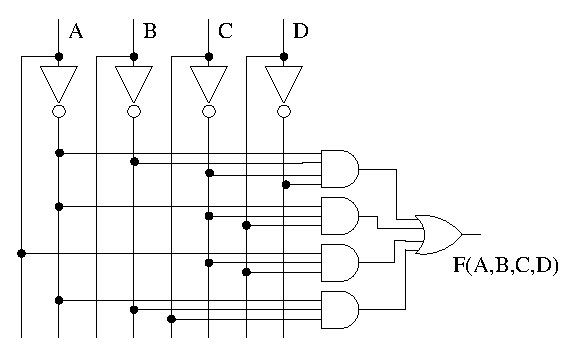
\includegraphics{./FigHw3/Prob3-3}}
\label{fig:Hw3}
\end{figure}

\begin{solution}{
From the circuit we have:
F(A,B,C,D) = A'B'C'D' + A'C'D + AC'D + A'B'C
$$ \begin{array} {c||c|c|c|c}
       AB \bs CD & 00 & 01 & 11 & 10 \\ \hline \hline
       00        & 1  & 1  & 1  & 1  \\ \hline
       01        &    & 1  &    &    \\ \hline
       11        &    & 1  &    &    \\ \hline
       10        &    & 1  &    &    \\
\end{array} $$ 
From this it follows that 
F(A,B,C,D) =  A'B' + C'D
} \end{solution}

\item  {\bf (8 pts.)} Design a digital system with four bits of inputs 
$I_3 I_2 I_1 I_0$ and two bits of outputs $O_1 O_0$.  At least one
of the inputs is always equal to 1.  The output encodes the 
index of the most significant 1 in the input.
For example, if $I_3 I_2 I_1 I_0 = 0101$, then the index
of the most significant 1 is 2, hence $O_1 O_0 = 10$.  Submit:
\begin{itemize}
\item The truth table.

\begin{solution}{
	\begin{tabular}{l|l|l|l||l|l}
	$I_3$ & $I_2$ & $I_1$ & $I_0$ & $O_1$ & $O_0$ \\ \hline
	0 & 0 & 0 & 0 &  x & x \\ \hline
	0 & 0 & 0 & 1 &  0 & 0 \\ \hline
	0 & 0 & 1 & 0 &  0 & 1 \\ \hline
	0 & 0 & 1 & 1 &  0 & 1 \\ \hline
	0 & 1 & 0 & 0 &  1 & 0 \\ \hline
	0 & 1 & 0 & 1 &  1 & 0 \\ \hline
	0 & 1 & 1 & 0 &  1 & 0 \\ \hline
	0 & 1 & 1 & 1 &  1 & 0 \\ \hline
	1 & 0 & 0 & 0 &  1 & 1 \\ \hline
	1 & 0 & 0 & 1 &  1 & 1 \\ \hline
	1 & 0 & 1 & 0 &  1 & 1 \\ \hline
	1 & 0 & 1 & 1 &  1 & 1 \\ \hline
	1 & 1 & 0 & 0 &  1 & 1 \\ \hline
	1 & 1 & 0 & 1 &  1 & 1 \\ \hline
	1 & 1 & 1 & 0 &  1 & 1 \\ \hline
	1 & 1 & 1 & 1 &  1 & 1 \\ 
	\end{tabular}
} \end{solution}
\item \SOPmin expression for $O_1$ and $O_0$.

\begin{solution}{
\begin{tabular}{ll}
$ \begin{array} {c||c|c|c|c}
 I3 I2 \bs I1 I0 & 00 & 01 & 11 & 10 \\ \hline \hline
       00        & x  &    &    &    \\ \hline
       01        & 1  & 1  & 1  & 1  \\ \hline
       11        & 1  & 1  & 1  & 1  \\ \hline
       10        & 1  & 1  & 1  & 1  \\
\end{array} $ & 
$ \begin{array} {c||c|c|c|c}
 I3 I2 \bs I1 I0 & 00 & 01 & 11 & 10 \\ \hline \hline
       00        & x  &    & 1  & 1  \\ \hline
       01        &    &    &    &    \\ \hline
       11        & 1  & 1  & 1  & 1  \\ \hline
       10        & 1  & 1  & 1  & 1  \\
\end{array} $ \\
$O_1 = I_3 + I_2$ & $O_0=I_3 + I_2'I_1$ \\
\end{tabular}
} \end{solution}
\end{itemize}

\item {\bf (8 pts.)}
Design a 4-input $a_1 a_0 b_1 b_0$, 4 -output $O_3 O_2 O_1 O_0$
digital system.  $A=a_1 a_0$ and $B=b_1 b_0$ represent 2-bit binary
numbers.  The output should be the product (multiplication) of the inputs, 
that is $O = A*B$.  In addition to determining the output, determine the
number of bits of output. Submit:
\begin{itemize}
\item Truth tables.

\begin{solution}{
\begin{tabular}{l|l|l|l||l|l|l|l}
$a_1$ & $a_0$ & $b_1$ & $b_0$ & $O_3$ & $O_2$ & $O_1$ & $O_0$ \\ \hline
0&0&0&0 &0&0&0&0 \\ \hline
0&0&0&1 &0&0&0&0 \\ \hline
0&0&1&0 &0&0&0&0 \\ \hline
0&0&1&1 &0&0&0&0 \\ \hline
0&1&0&0 &0&0&0&0 \\ \hline
0&1&0&1 &0&0&0&1 \\ \hline
0&1&1&0 &0&0&1&0 \\ \hline
0&1&1&1 &0&0&1&1 \\ \hline
1&0&0&0 &0&0&0&0 \\ \hline
1&0&0&1 &0&0&1&0 \\ \hline
1&0&1&0 &0&1&0&0 \\ \hline
1&0&1&1 &0&1&1&0 \\ \hline
1&1&0&0 &0&0&0&0 \\ \hline
1&1&0&1 &0&0&1&1 \\ \hline
1&1&1&0 &0&1&1&0 \\ \hline
1&1&1&1 &1&0&0&1 \\
\end{tabular}
} \end{solution}

\item Minimal SOP expression for the outputs.

\begin{solution}{
\begin{tabular}{ll}
$\begin{array} {c||c|c|c|c}
 a1 a0 \bs b1 b0 & 00 & 01 & 11 & 10 \\ \hline \hline
       00        &    &    &    &    \\ \hline
       01        &    &    &    &    \\ \hline
       11        &    &    & 1  &    \\ \hline
       10        &    &    &    &    \\
\end{array}$ &
$\begin{array} {c||c|c|c|c}
 a1 a0 \bs b1 b0 & 00 & 01 & 11 & 10 \\ \hline \hline
       00        &    &    &    &    \\ \hline
       01        &    &    &    &    \\ \hline
       11        &    &    &    & 1  \\ \hline
       10        &    &    & 1  & 1  \\
\end{array} $ \\
$O_3 = a_1a_0b_1b_0$ & $O_2 = a_1a_0'b_1 + a_1b_1b_0'$\\
\end{tabular}
} \end{solution}


\begin{solution}{
\begin{tabular}{ll}
$\begin{array} {c||c|c|c|c}
 a1 a0 \bs b1 b0 & 00 & 01 & 11 & 10 \\ \hline \hline
       00        &    &    &    &    \\ \hline
       01        &    &    & 1  & 1  \\ \hline
       11        &    & 1  &    & 1  \\ \hline
       10        &    & 1  & 1  &    \\
\end{array}$ &
$\begin{array} {c||c|c|c|c}
 a1 a0 \bs b1 b0 & 00 & 01 & 11 & 10 \\ \hline \hline
       00        &    &    &    &    \\ \hline
       01        &    & 1  & 1  &    \\ \hline
       11        &    & 1  & 1  &    \\ \hline
       10        &    &    &    &    \\
\end{array}$ \\
$O_1 = a_1b_1'b_0 + a_1a_0'b_0 + a_1'a_0b_1+a_0b_1b_0'$ & $O_0 = a_0b_0$ \\
\end{tabular}
} \end{solution}

\end{itemize}

\item  {\bf (8 pts.)}
Design a 4-bit Gray-code to binary converter.  A 4-bit gray-code is a 
sequence of 4-bit values where successive values differ by a single
bit.  For this problem use the sequence: 0000, 0001, 0011, 0010, 
0110, 0111, 0101, 0100, 1100, 1101, 1111, 1110, 1010, 1011, 1001, 
1000.  The index of the 4-bit gray code is its binary value.  For
example, the 4-bit gray code 0111 is at index 5, therefore when
presented with 0111 on its input, the converter should output 0101.
Submit:
\begin{itemize}
\item A truth table for the converter.

\begin{solution}{
\begin{tabular}{l|l|l|l||l|l|l|l}
$a_3$ & $a_2$ & $a_1$ & $a_0$ & $f_3$ & $f_2$ & $f_1$ & $f_0$ \\ \hline
0&0&0&0 &0&0&0&0 \\ \hline
0&0&0&1 &0&0&0&1 \\ \hline
0&0&1&0 &0&0&1&1 \\ \hline
0&0&1&1 &0&0&1&0 \\ \hline
0&1&0&0 &0&1&1&0 \\ \hline
0&1&0&1 &0&1&1&1 \\ \hline
0&1&1&0 &0&1&0&1 \\ \hline
0&1&1&1 &0&1&0&0 \\ \hline
1&0&0&0 &1&1&0&0 \\ \hline
1&0&0&1 &1&1&0&1 \\ \hline
1&0&1&0 &1&1&1&1 \\ \hline
1&0&1&1 &1&1&1&0 \\ \hline
1&1&0&0 &1&0&1&0 \\ \hline
1&1&0&1 &1&0&1&1 \\ \hline
1&1&1&0 &1&0&0&1 \\ \hline
1&1&1&1 &1&0&0&0 \\ 
\end{tabular}
} \end{solution}

\item Four k-maps for the converter.

\begin{solution}{
\begin{tabular}{ll}
$\begin{array} {c||c|c|c|c}
 a3 a2 \bs a1 a0 & 00 & 01 & 11 & 10 \\ \hline \hline
       00        &    &    &    &    \\ \hline
       01        &    &    &    &    \\ \hline
       11        & 1  & 1  & 1  & 1  \\ \hline
       10        & 1  & 1  & 1  & 1  \\
\end{array}$ &
$\begin{array} {c||c|c|c|c}
 a3 a2 \bs a1 a0 & 00 & 01 & 11 & 10 \\ \hline \hline
       00        &    &    &    &    \\ \hline
       01        & 1  & 1  & 1  & 1  \\ \hline
       11        &    &    &    &    \\ \hline
       10        & 1  & 1  & 1  & 1  \\
\end{array} $ \\
$f_3 = a_3$ & $f_2 = a_3a_2'+a_3'a_2$\\
\end{tabular}
} \end{solution}


\begin{solution}{
\begin{tabular}{ll}
$\begin{array} {c||c|c|c|c}
 a3 a2 \bs a1 a0 & 00 & 01 & 11 & 10 \\ \hline \hline
       00        &    &    & 1  & 1  \\ \hline
       01        & 1  & 1  &    &    \\ \hline
       11        & 1  & 1  &    &    \\ \hline
       10        &    &    & 1  & 1  \\
\end{array}$ &
$\begin{array} {c||c|c|c|c}
 a3 a2 \bs a1 a0 & 00 & 01 & 11 & 10 \\ \hline \hline
       00        &    & 1  &    & 1  \\ \hline
       01        &    & 1  &    & 1  \\ \hline
       11        &    & 1  &    & 1  \\ \hline
       10        &    & 1  &    & 1  \\
\end{array}$ \\
$f_1 = a_2a_1'+a_2'a_1$ & $f_0 = a_1'a_0+a_1a_0'$ \\
\end{tabular}
} \end{solution}

\item \SOPmin expression for the outputs, no product sharing please
(use the \verb+-Dso+ command line option).
\item Espresso file for the converter
\item Espresso output in PLA format
\item Compare the number of gates required in your solution
versus the number of gates required by Espresso.
\end{itemize}

\item {\bf (4 pts. each)} Determine \SOPmin expression for:
\begin{enumerate}
\item $F(A,B,C)=\sum m(0,1,3,4,5)$

\begin{solution}{
$\begin{array} {c||c|c|c|c}
   A   \bs B C  & 00 & 01 & 11 & 10 \\ \hline \hline
       0        &  1 & 1  & 1  &    \\ \hline
       1        &  1 & 1  &    &    \\ 
\end{array}$ \\
F(A,B,C)= B'+A'C
} \end{solution}
\item $F(A,B,C,D)=\sum m(1,5,6,7,11,12,13,15)$

\begin{solution}{
$\begin{array} {c||c|c|c|c}
   A B \bs C D   & 00 & 01 & 11 & 10 \\ \hline \hline
       00        &    & 1  &    &    \\ \hline
       01        &    & 1  & 1  & 1  \\ \hline
       11        & 1  & 1  & 1  &    \\ \hline
       10        &    &    & 1  &    \\
\end{array}$  \\
F(A,B,C)= ABC'+A'C'D+ACD+A'BC
} \end{solution}
\item $F(A,B,C,D)=\sum m(0,2,5,6,8,11,12,13,14,15)$

\begin{solution}{
$\begin{array} {c||c|c|c|c}
   A B \bs C D   & 00 & 01 & 11 & 10 \\ \hline \hline
       00        & 1  &    &    & 1  \\ \hline
       01        &    & 1  &    & 1  \\ \hline
       11        & 1  & 1  & 1  & 1  \\ \hline
       10        & 1  &    & 1  &    \\
\end{array}$  \\
F(A,B,C,D) =  AB + BC'D + ACD + B'C'D' + A'CD'
} \end{solution}
\item $F(A,B,C,D,E)=\sum m(0,8,9,10,13,15,22,26,29,30,31)$

\begin{solution}{
\begin{tabular}{cc}
$\begin{array} {c||c|c|c|c}
   B C \bs D E   & 00 & 01 & 11 & 10 \\ \hline \hline
       00        & 1  &    &    &    \\ \hline
       01        &    &    &    &    \\ \hline
       11        &    & 1  & 1  &    \\ \hline
       10        & 1  & 1  &    & 1  \\
\end{array}$ &
$\begin{array} {c||c|c|c|c}
   B C \bs D E   & 00 & 01 & 11 & 10 \\ \hline \hline
       00        &    &    &    &    \\ \hline
       01        &    &    &    & 1  \\ \hline
       11        &    & 1  & 1  & 1  \\ \hline
       10        &    &    &    & 1  \\
\end{array}$ \\
A=0 & A=1 \\
\end{tabular} \\
F(A,B,C,D,E) = BCE + A'C'D'E' + BC'DE + ACDE' + A'BD'E or \\
F(A,B,C,D,E) = BCE + A'C'D'E' + BC'DE + ACDE' + A'BC'D'
} \end{solution}

\item $F(A,B,C,D,E)=\sum m(0,2,4,5,7,10,13,15,18,21,24,26,28,29)$

\begin{solution}{
\begin{tabular}{cc}
$\begin{array} {c||c|c|c|c}
   B C \bs D E   & 00 & 01 & 11 & 10 \\ \hline \hline
       00        & 1  &    &    & 1  \\ \hline
       01        & 1  & 1  & 1  &    \\ \hline
       11        &    & 1  & 1  &    \\ \hline
       10        &    &    &    & 1  \\
\end{array}$ &
$\begin{array} {c||c|c|c|c}
   B C \bs D E   & 00 & 01 & 11 & 10 \\ \hline \hline
       00        &    &    &    & 1  \\ \hline
       01        &    & 1  &    &    \\ \hline
       11        & 1  & 1  &    &    \\ \hline
       10        & 1  &    &    & 1  \\
\end{array}$ \\
A=0 & A=1 \\
\end{tabular} \\
F(A,B,C,D,E) = A'B'D'E' + CD'E+C'DE'+ABD'E'+A'CE
} \end{solution}

\end{enumerate}

\item {\bf (4 pts. each)} Determine \SOPmin expression for:
\begin{enumerate}
\item $F(A,B,C,D)=\sum m(4,7,9,12,13,15)+\sum d(0,1,2,3,10,14)$

\begin{solution}{
$\begin{array} {c||c|c|c|c}
   A B \bs C D   & 00 & 01 & 11 & 10 \\ \hline \hline
       00        & x  & x  & x  &    \\ \hline
       01        & 1  &    & 1  &    \\ \hline
       11        & 1  & 1  & 1  & x  \\ \hline
       10        &    & 1  &    & x  \\
\end{array}$  \\
F(A,B,C,D) = BC'D'+AC'D+BCD
} \end{solution}

\item $F(A,B,C,D)=\sum m(0,1,5,7,10,14,15)+\sum d(2,8)$

\begin{solution}{
$\begin{array} {c||c|c|c|c}
   A B \bs C D   & 00 & 01 & 11 & 10 \\ \hline \hline
       00        & 1  & 1  &    & x  \\ \hline
       01        &    & 1  & 1  &    \\ \hline
       11        &    &    & 1  & 1  \\ \hline
       10        & x  &    &    & 1  \\
\end{array}$ \\
F(A,B,C,D) = B'D'+A'C'D+BCD+ABC
} \end{solution}
\item $F(A,B,C,D)=\sum m(0,1,3,4,15)+\sum d(10,12)$

\begin{solution}{

$\begin{array} {c||c|c|c|c}
   A B \bs C D   & 00 & 01 & 11 & 10 \\ \hline \hline
       00        & 1  & 1  & 1  &    \\ \hline
       01        & 1  &    &    &    \\ \hline
       11        & x  &    & 1  &    \\ \hline
       10        &    &    &    & x  \\
\end{array}$ \\
F(A,B,C,D)=ABCD+A'C'D'+A'B'D
} \end{solution}
\item $F(A,B,C,D,E)=\sum m(2,3,5,7,11,13,17,19,29,31)+\sum d(1,4,9,16,25)$

\begin{solution}{

\begin{tabular}{cc}
$\begin{array} {c||c|c|c|c}
   B C \bs D E   & 00 & 01 & 11 & 10 \\ \hline \hline
       00        &    & x  & 1  & 1  \\ \hline
       01        & x  & 1  & 1  &    \\ \hline
       11        &    & 1  &    &    \\ \hline
       10        &    & x  & 1  &    \\
\end{array}$ &
$\begin{array} {c||c|c|c|c}
   B C \bs D E   & 00 & 01 & 11 & 10 \\ \hline \hline
       00        & x  & 1  & 1  &    \\ \hline
       01        &    &    &    &    \\ \hline
       11        &    & 1  & 1  &    \\ \hline
       10        &    & x  &    &    \\
\end{array}$ \\
A=0 & A=1 \\
\end{tabular} \\
F(A,B,C,D,E)=A'D'E+A'C'E+A'B'C'D+B'C'E+ABCE +A'B'E
} \end{solution}

\item $F(A,B,C,D,E)=\sum m(2,3,6,10,12,13,14,18,25,26,28,29)+\sum d(11,27)$

\begin{solution}{

\begin{tabular}{cc}
$\begin{array} {c||c|c|c|c}
   B C \bs D E   & 00 & 01 & 11 & 10 \\ \hline \hline
       00        &    &    & 1  & 1  \\ \hline
       01        &    &    &    & 1  \\ \hline
       11        & 1  & 1  &    & 1  \\ \hline
       10        &    &    & x  & 1  \\
\end{array}$ &
$\begin{array} {c||c|c|c|c}
   B C \bs D E   & 00 & 01 & 11 & 10 \\ \hline \hline
       00        &    &    &    & 1  \\ \hline
       01        &    &    &    &    \\ \hline
       11        & 1  & 1  &    &    \\ \hline
       10        &    & 1  & x  & 1  \\
\end{array}$ \\
A=0 & A=1 \\
\end{tabular} \\
F(A,B,C,D,E)=A'C'D+C'DE'+A'DE' +BCD' + ABC'E 
} \end{solution}

\end{enumerate}

\item {\bf (8 pts. each)} Determine \SOPmin and \POSmin expressions for:
\begin{enumerate}
\item  $F(A,B,C,D) = \sum m(0,1,2,5,8,10,13,15)$

\begin{solution}{

\begin{tabular}{cc}
$\begin{array} {c||c|c|c|c}
   A B \bs C D   & 00 & 01 & 11 & 10 \\ \hline \hline
       00        & 1  & 1  &    & 1  \\ \hline
       01        &    & 1  &    &    \\ \hline
       11        &    & 1  & 1  &    \\ \hline
       10        & 1  &    &    & 1  \\
\end{array}$ &
$\begin{array} {c||c|c|c|c}
   A B \bs C D   & 00 & 01 & 11 & 10 \\ \hline \hline
       00        &    &    & 1  &    \\ \hline
       01        & 1  &    & 1  & 1  \\ \hline
       11        & 1  &    &    & 1  \\ \hline
       10        &    & 1  & 1  &    \\
\end{array}$ \\
F  & F' \\
\end{tabular} \\
\SOPmin F(A,B,C,D) =  B'D'+A'C'D+ABD\\
\POSmin F(A,B,C,D) =  (B'+D)(A+C'+D')(A'+B+D')
} \end{solution}

\item  $F(A,B,C,D) = \prod M(0,4,6,10,11,12)$

\begin{solution}{

\begin{tabular}{cc}
$\begin{array} {c||c|c|c|c}
   A B \bs C D   & 00 & 01 & 11 & 10 \\ \hline \hline
       00        &    & 1  & 1  & 1  \\ \hline
       01        &    & 1  & 1  &    \\ \hline
       11        &    & 1  & 1  & 1  \\ \hline
       10        & 1  & 1  &    &    \\
\end{array}$ &
$\begin{array} {c||c|c|c|c}
   A B \bs C D   & 00 & 01 & 11 & 10 \\ \hline \hline
       00        & 1  &    &    &    \\ \hline
       01        & 1  &    &    & 1  \\ \hline
       11        & 1  &    &    &    \\ \hline
       10        &    &    & 1  & 1  \\
\end{array}$ \\
F  & F' \\
\end{tabular} \\
\SOPmin F(A,B,C,D) = AB'C'+A'B'C+ABC+C'D+A'D  or \\
\SOPmin F(A,B,C,D) = AB'C'+A'B'C+ABC+C'D+BD  or \\
\SOPmin F(A,B,C,D) = AB'C'+A'B'C+ABC+A'D+BD \\
\POSmin F(A,B,C,D) =  (A+C+D)(B'+C+D)(A+B'+D)(A'+B+C')
} \end{solution}
\item  $F(A,B,C,D) = \sum m(0,5,7,10,11,14) + \sum d(3,12,15)$

\begin{solution}{

\begin{tabular}{cc}
$\begin{array} {c||c|c|c|c}
   A B \bs C D   & 00 & 01 & 11 & 10 \\ \hline \hline
       00        & 1  &    & x  &    \\ \hline
       01        &    & 1  & 1  &    \\ \hline
       11        & x  &    & x  & 1  \\ \hline
       10        &    &    & 1  & 1  \\
\end{array}$ &
$\begin{array} {c||c|c|c|c}
   A B \bs C D   & 00 & 01 & 11 & 10 \\ \hline \hline
       00        &    & 1  & x  & 1  \\ \hline
       01        & 1  &    &    & 1  \\ \hline
       11        & x  & 1  & x  &    \\ \hline
       10        & 1  & 1  &    &    \\
\end{array}$ \\
F  & F' \\
\end{tabular} \\
\SOPmin F(A,B,C,D) =  A'B'C'D'+A'BD+AC\\
\POSmin F(A,B,C,D) =  (A'+C)(A+C'+D)(A+B+D')(B'+C+D) or \\ 
\POSmin F(A,B,C,D) =  (A'+C)(A+C'+D)(B+C+D')(B'+C+D) or \\ 
\POSmin F(A,B,C,D) =  (A'+C)(A+C'+D)(A+B+D')(A+B'+D) or \\ 
\POSmin F(A,B,C,D) =  (A'+C)(A+C'+D)(B+C+D')(A+B'+D)  \\ 
} \end{solution}
\item  $F(A,B,C,D) = \prod M(2,6,7,9,15) * \prod d(4,12,13) $

\begin{solution}{

\begin{tabular}{cc}
$\begin{array} {c||c|c|c|c}
   A B \bs C D   & 00 & 01 & 11 & 10 \\ \hline \hline
       00        & 1  & 1  & 1  &    \\ \hline
       01        & x  & 1  &    &    \\ \hline
       11        & x  & x  &    & 1  \\ \hline
       10        & 1  &    & 1  & 1  \\
\end{array}$ &
$\begin{array} {c||c|c|c|c}
   A B \bs C D   & 00 & 01 & 11 & 10 \\ \hline \hline
       00        &    &    &    & 1  \\ \hline
       01        & x  &    & 1  & 1  \\ \hline
       11        & x  & x  & 1  &    \\ \hline
       10        &    & 1  &    &    \\
\end{array}$ \\
F  & F' \\
\end{tabular} \\
\SOPmin F(A,B,C,D) =  A'C'+AD'+A'CD\\
\POSmin F(A,B,C,D) =  (A+C'+D)(B'+C'+D')(A'+C+D')
} \end{solution}
\item  $F(W,X,Y,Z) = WX'Z' + X'YZ + W'Y'Z + XYZ + WXY'$

\begin{solution}{
\begin{tabular}{cc}
$\begin{array} {c||c|c|c|c}
   W X \bs Y Z   & 00 & 01 & 11 & 10 \\ \hline \hline
       00        &    & 1  & 1  &    \\ \hline
       01        &    & 1  & 1  &    \\ \hline
       11        & 1  & 1  & 1  &    \\ \hline
       10        & 1  &    & 1  & 1  \\
\end{array}$ &
$\begin{array} {c||c|c|c|c}
   W X \bs Y Z   & 00 & 01 & 11 & 10 \\ \hline \hline
       00        & 1  &    &    & 1  \\ \hline
       01        & 1  &    &    & 1  \\ \hline
       11        &    &    &    & 1  \\ \hline
       10        &    & 1  &    &    \\
\end{array}$ \\
F  & F' \\
\end{tabular} \\
\SOPmin F(W,X,Y,Z) =  W'Z+XZ+WY'Z'+WX'Y\\
\POSmin F(W,X,Y,Z) = (W+Z)(X'+Y'+Z)(W'+X+Y+Z')
} \end{solution}

\item  $F(W,X,Y,Z) = (W + X'+Y')(W'+Z')(W+Y')$

\begin{solution}{

We have that $F'(W,X,Y,Z) = W'XY+ WZ+ W'Y$

\begin{tabular}{cc}
$\begin{array} {c||c|c|c|c}
   W X \bs Y Z   & 00 & 01 & 11 & 10 \\ \hline \hline
       00        &    &    & 1  & 1  \\ \hline
       01        &    &    & 1  & 1  \\ \hline
       11        &    & 1  & 1  &    \\ \hline
       10        &    & 1  & 1  &    \\
\end{array}$ &
$\begin{array} {c||c|c|c|c}
   W X \bs Y Z   & 00 & 01 & 11 & 10 \\ \hline \hline
       00        & 1  & 1  &    &    \\ \hline
       01        & 1  & 1  &    &    \\ \hline
       11        & 1  &    &    & 1  \\ \hline
       10        & 1  &    &    & 1  \\
\end{array}$ \\
F'  & F \\
\end{tabular} \\
\SOPmin F(W,X,Y,Z) =  W'Y'+WZ'\\
\POSmin F(W,X,Y,Z) = (W'+Z')(W+Y')
} \end{solution}
\end{enumerate}
Hint, the negation of a ``Don't care" is a ``Don't care".

\item {\bf (3 pts.)} While grading homework for a digital design class 
the following question/answer pair is encountered.  What is 
the problem with the answer given?

\begin{tabular}{l}
Question: Generate the \POSmin expression for $F(A,B,C) = \sum m(2,3,4,5)$ \\
Answer: $F(A,B,C) = (A+B')(A'+B)$ \\
\end{tabular}

\item {\bf (6 pts.)} Determine the \SOPmin realization of the following
function.

\begin{tabular}{c|c|c|c||c}
A & B & C & D & F(A,B,C,D) \\ \hline
x & 1 & 1 & x & 0 \\ \hline
0 & x & 0 & 1 & 0 \\ \hline
x & x & 0 & 0 & x \\ \hline
x & 0 & 1 & x & 1 \\ \hline
1 & x & 0 & 1 & 1 \\ 
\end{tabular}


\begin{solution}{
$\begin{array} {c||c|c|c|c}
   A B \bs B C   & 00 & 01 & 11 & 10 \\ \hline \hline
       00        & x  & 0  & 1  & 1  \\ \hline
       01        & x  & 0  & 0  & 0  \\ \hline
       11        & x  & 1  & 0  & 0  \\ \hline
       10        & x  & 1  & 1  & 1  \\
\end{array}$  \\
F(A,B,C) = AC'+B'C
} \end{solution}

\item {\bf (6 pts.)} What is the worst function \SOPmin of 3 variable 
that can be created?  That is, define a function whose minimal SOP form 
has the largest possible number of product terms.  What is the largest 
number of product terms that a 4-variable \SOPmin expression can 
have?  How about $N$ variables?

\begin{solution}{
The worst function of three variable is shown in the Kmap below:

$\begin{array} {c||c|c|c|c}
   A \bs B C   & 00 & 01 & 11 & 10 \\ \hline \hline
      0        & 1  &    & 1  &    \\ \hline
      1        &    & 1  &    & 1  \\ 
\end{array}$

This function requires four product terms.  Any additional minterm added to 
this Kmap would create a grouping with neighboring minterms, perhaps not 
decreasing the
the number of product terms, but certainly making the product terms simpler.
Its important to note that this configuration looks like a checkerboard.
The worst function of four variables looks like:

$\begin{array} {c||c|c|c|c}
   A B \bs B C   & 00 & 01 & 11 & 10 \\ \hline \hline
       00        & 1  &    & 1  &    \\ \hline
       01        &    & 1  &    & 1  \\ \hline
       11        & 1  &    & 1  &    \\ \hline
       10        &    & 1  &    & 1  \\
\end{array}$

This function requires 8 product terms, each containing every variable.  Boy that's
one bad realization.  In a general, the worst realization of an $N$ variable function 
requires $2^{N-1}$ product terms.  This is because the checkerboard configuration can
be applied to any Kmap, with half of the cells containing 1's.  Since a function with
$N$ variables has $2^{N}$ cells, then 1/2 of these cells works out to $2^{N-1}$.
} \end{solution} 


\item {\bf (16 pts.)} Sometimes a logic circuit needs to output 
a logic 0 in order to produce some behavior.  For example, an LED can be
attached to a digital circuit output so that it lights up when the circuit
outputs a 0.  This response is called an active low output; the output
device is {\it active} then the digital output is {\it low}.
                                                                                
Build a digital circuit that takes as input two 2-bit numbers,
A and B.  The circuit has three outputs which drive three
LEDs labeled G, L, and E.
The G LED should be illuminated when A$>$B.
The L LED should be illuminated when A$<$B.
The E LED should be illuminated when A=B.
The LEDs are illuminated when the circuit outputs a 0, otherwise
they are turned off.
                                                                                
Determine \SOPmin expression for the G, L and E outputs.
Determine \POSmin expression for the G, L and E outputs.
                                                                                


\end{enumerate}


\begin{enumerate}
\item {\bf (6 pts.)} Design a circuit called DECODE.  DECODE has two bits of 
input $S, D$ and two bit of output $y_1 y_0$.  If $S=0$ then $y_0=D$ and 
$y_1=0$ else if $S=1$ then $y_0=0$ and $y_1 = D$.
\begin{enumerate}
        \item Write down the truth table for the DECODE function.


\begin{solution}{
	\begin{tabular}{l|l||l|l}
	S & D & $y_1$ & $y_0$ \\ \hline
	0 & 0 & 0   & 0   \\ \hline
	0 & 1 & 0   & 1   \\ \hline
	0 & 0 & 0   & 0   \\ \hline
	1 & 1 & 1   & 0   \\ 
	\end{tabular}
} \end{solution}
        \item Determine the \SOPmin realization for DECODE.


\begin{solution}{
$y_0 = S'D$\\
$y_1 = S D$
} \end{solution}
\end{enumerate}

\item {\bf (6 pts.)} Design a circuit called FULLADD.  FULLADD has 
three bits of input $a,b,c$ and two bits of output $s_1 s_0$.  The output 
represents the sum of the three bits.
\begin{enumerate}
        \item Write down the truth table for the FULLADD function.


\begin{solution}{
	\begin{tabular}{l|l|l|l|l}
	a & b & c & $s_1$ & $s_0$ \\ \hline
	0 & 0 & 0 & 0   & 0   \\ \hline
	0 & 0 & 1 & 0   & 1   \\ \hline
	0 & 1 & 0 & 0   & 0   \\ \hline
	0 & 1 & 1 & 1   & 1   \\ \hline
	1 & 0 & 0 & 0   & 0   \\ \hline
	1 & 0 & 1 & 1   & 1   \\ \hline
	1 & 1 & 0 & 1   & 0   \\ \hline
	1 & 1 & 1 & 1   & 1   \\ 
\end{tabular}
} \end{solution}
        \item Determine the \SOPmin realization for FULLADD.

\begin{solution}{
$s_1 = ab + ac + bc $ \\
$s_0 = a'b'c + a'bc' + ab'c' + abc $
} \end{solution}
\end{enumerate}

\item  {\bf (4 pts.)} Determine \SOPmin expression for the following circuit
and draw the circuit using the fewest number of gates possible.
\begin{figure}[ht]
%% scalebox
\center{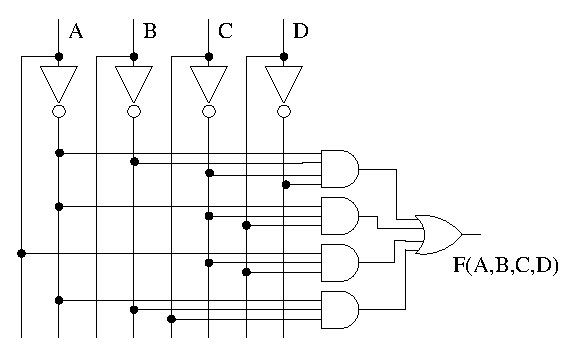
\includegraphics{./FigHw3/Prob3-3}}
\label{fig:Hw3}
\end{figure}

\begin{solution}{
From the circuit we have:
F(A,B,C,D) = A'B'C'D' + A'C'D + AC'D + A'B'C
$$ \begin{array} {c||c|c|c|c}
       AB \bs CD & 00 & 01 & 11 & 10 \\ \hline \hline
       00        & 1  & 1  & 1  & 1  \\ \hline
       01        &    & 1  &    &    \\ \hline
       11        &    & 1  &    &    \\ \hline
       10        &    & 1  &    &    \\
\end{array} $$ 
From this it follows that 
F(A,B,C,D) =  A'B' + C'D
} \end{solution}

\item  {\bf (8 pts.)} Design a digital system with four bits of inputs 
$I_3 I_2 I_1 I_0$ and two bits of outputs $O_1 O_0$.  At least one
of the inputs is always equal to 1.  The output encodes the 
index of the most significant 1 in the input.
For example, if $I_3 I_2 I_1 I_0 = 0101$, then the index
of the most significant 1 is 2, hence $O_1 O_0 = 10$.  Submit:
\begin{itemize}
\item The truth table.

\begin{solution}{
	\begin{tabular}{l|l|l|l||l|l}
	$I_3$ & $I_2$ & $I_1$ & $I_0$ & $O_1$ & $O_0$ \\ \hline
	0 & 0 & 0 & 0 &  x & x \\ \hline
	0 & 0 & 0 & 1 &  0 & 0 \\ \hline
	0 & 0 & 1 & 0 &  0 & 1 \\ \hline
	0 & 0 & 1 & 1 &  0 & 1 \\ \hline
	0 & 1 & 0 & 0 &  1 & 0 \\ \hline
	0 & 1 & 0 & 1 &  1 & 0 \\ \hline
	0 & 1 & 1 & 0 &  1 & 0 \\ \hline
	0 & 1 & 1 & 1 &  1 & 0 \\ \hline
	1 & 0 & 0 & 0 &  1 & 1 \\ \hline
	1 & 0 & 0 & 1 &  1 & 1 \\ \hline
	1 & 0 & 1 & 0 &  1 & 1 \\ \hline
	1 & 0 & 1 & 1 &  1 & 1 \\ \hline
	1 & 1 & 0 & 0 &  1 & 1 \\ \hline
	1 & 1 & 0 & 1 &  1 & 1 \\ \hline
	1 & 1 & 1 & 0 &  1 & 1 \\ \hline
	1 & 1 & 1 & 1 &  1 & 1 \\ 
	\end{tabular}
} \end{solution}
\item \SOPmin expression for $O_1$ and $O_0$.

\begin{solution}{
\begin{tabular}{ll}
$ \begin{array} {c||c|c|c|c}
 I3 I2 \bs I1 I0 & 00 & 01 & 11 & 10 \\ \hline \hline
       00        & x  &    &    &    \\ \hline
       01        & 1  & 1  & 1  & 1  \\ \hline
       11        & 1  & 1  & 1  & 1  \\ \hline
       10        & 1  & 1  & 1  & 1  \\
\end{array} $ & 
$ \begin{array} {c||c|c|c|c}
 I3 I2 \bs I1 I0 & 00 & 01 & 11 & 10 \\ \hline \hline
       00        & x  &    & 1  & 1  \\ \hline
       01        &    &    &    &    \\ \hline
       11        & 1  & 1  & 1  & 1  \\ \hline
       10        & 1  & 1  & 1  & 1  \\
\end{array} $ \\
$O_1 = I_3 + I_2$ & $O_0=I_3 + I_2'I_1$ \\
\end{tabular}
} \end{solution}
\end{itemize}

\item {\bf (8 pts.)}
Design a 4-input $a_1 a_0 b_1 b_0$, 4 -output $O_3 O_2 O_1 O_0$
digital system.  $A=a_1 a_0$ and $B=b_1 b_0$ represent 2-bit binary
numbers.  The output should be the product (multiplication) of the inputs, 
that is $O = A*B$.  In addition to determining the output, determine the
number of bits of output. Submit:
\begin{itemize}
\item Truth tables.

\begin{solution}{
\begin{tabular}{l|l|l|l||l|l|l|l}
$a_1$ & $a_0$ & $b_1$ & $b_0$ & $O_3$ & $O_2$ & $O_1$ & $O_0$ \\ \hline
0&0&0&0 &0&0&0&0 \\ \hline
0&0&0&1 &0&0&0&0 \\ \hline
0&0&1&0 &0&0&0&0 \\ \hline
0&0&1&1 &0&0&0&0 \\ \hline
0&1&0&0 &0&0&0&0 \\ \hline
0&1&0&1 &0&0&0&1 \\ \hline
0&1&1&0 &0&0&1&0 \\ \hline
0&1&1&1 &0&0&1&1 \\ \hline
1&0&0&0 &0&0&0&0 \\ \hline
1&0&0&1 &0&0&1&0 \\ \hline
1&0&1&0 &0&1&0&0 \\ \hline
1&0&1&1 &0&1&1&0 \\ \hline
1&1&0&0 &0&0&0&0 \\ \hline
1&1&0&1 &0&0&1&1 \\ \hline
1&1&1&0 &0&1&1&0 \\ \hline
1&1&1&1 &1&0&0&1 \\
\end{tabular}
} \end{solution}

\item Minimal SOP expression for the outputs.

\begin{solution}{
\begin{tabular}{ll}
$\begin{array} {c||c|c|c|c}
 a1 a0 \bs b1 b0 & 00 & 01 & 11 & 10 \\ \hline \hline
       00        &    &    &    &    \\ \hline
       01        &    &    &    &    \\ \hline
       11        &    &    & 1  &    \\ \hline
       10        &    &    &    &    \\
\end{array}$ &
$\begin{array} {c||c|c|c|c}
 a1 a0 \bs b1 b0 & 00 & 01 & 11 & 10 \\ \hline \hline
       00        &    &    &    &    \\ \hline
       01        &    &    &    &    \\ \hline
       11        &    &    &    & 1  \\ \hline
       10        &    &    & 1  & 1  \\
\end{array} $ \\
$O_3 = a_1a_0b_1b_0$ & $O_2 = a_1a_0'b_1 + a_1b_1b_0'$\\
\end{tabular}
} \end{solution}


\begin{solution}{
\begin{tabular}{ll}
$\begin{array} {c||c|c|c|c}
 a1 a0 \bs b1 b0 & 00 & 01 & 11 & 10 \\ \hline \hline
       00        &    &    &    &    \\ \hline
       01        &    &    & 1  & 1  \\ \hline
       11        &    & 1  &    & 1  \\ \hline
       10        &    & 1  & 1  &    \\
\end{array}$ &
$\begin{array} {c||c|c|c|c}
 a1 a0 \bs b1 b0 & 00 & 01 & 11 & 10 \\ \hline \hline
       00        &    &    &    &    \\ \hline
       01        &    & 1  & 1  &    \\ \hline
       11        &    & 1  & 1  &    \\ \hline
       10        &    &    &    &    \\
\end{array}$ \\
$O_1 = a_1b_1'b_0 + a_1a_0'b_0 + a_1'a_0b_1+a_0b_1b_0'$ & $O_0 = a_0b_0$ \\
\end{tabular}
} \end{solution}

\end{itemize}

\item  {\bf (8 pts.)}
Design a 4-bit Gray-code to binary converter.  A 4-bit gray-code is a 
sequence of 4-bit values where successive values differ by a single
bit.  For this problem use the sequence: 0000, 0001, 0011, 0010, 
0110, 0111, 0101, 0100, 1100, 1101, 1111, 1110, 1010, 1011, 1001, 
1000.  The index of the 4-bit gray code is its binary value.  For
example, the 4-bit gray code 0111 is at index 5, therefore when
presented with 0111 on its input, the converter should output 0101.
Submit:
\begin{itemize}
\item A truth table for the converter.

\begin{solution}{
\begin{tabular}{l|l|l|l||l|l|l|l}
$a_3$ & $a_2$ & $a_1$ & $a_0$ & $f_3$ & $f_2$ & $f_1$ & $f_0$ \\ \hline
0&0&0&0 &0&0&0&0 \\ \hline
0&0&0&1 &0&0&0&1 \\ \hline
0&0&1&0 &0&0&1&1 \\ \hline
0&0&1&1 &0&0&1&0 \\ \hline
0&1&0&0 &0&1&1&0 \\ \hline
0&1&0&1 &0&1&1&1 \\ \hline
0&1&1&0 &0&1&0&1 \\ \hline
0&1&1&1 &0&1&0&0 \\ \hline
1&0&0&0 &1&1&0&0 \\ \hline
1&0&0&1 &1&1&0&1 \\ \hline
1&0&1&0 &1&1&1&1 \\ \hline
1&0&1&1 &1&1&1&0 \\ \hline
1&1&0&0 &1&0&1&0 \\ \hline
1&1&0&1 &1&0&1&1 \\ \hline
1&1&1&0 &1&0&0&1 \\ \hline
1&1&1&1 &1&0&0&0 \\ 
\end{tabular}
} \end{solution}

\item Four k-maps for the converter.

\begin{solution}{
\begin{tabular}{ll}
$\begin{array} {c||c|c|c|c}
 a3 a2 \bs a1 a0 & 00 & 01 & 11 & 10 \\ \hline \hline
       00        &    &    &    &    \\ \hline
       01        &    &    &    &    \\ \hline
       11        & 1  & 1  & 1  & 1  \\ \hline
       10        & 1  & 1  & 1  & 1  \\
\end{array}$ &
$\begin{array} {c||c|c|c|c}
 a3 a2 \bs a1 a0 & 00 & 01 & 11 & 10 \\ \hline \hline
       00        &    &    &    &    \\ \hline
       01        & 1  & 1  & 1  & 1  \\ \hline
       11        &    &    &    &    \\ \hline
       10        & 1  & 1  & 1  & 1  \\
\end{array} $ \\
$f_3 = a_3$ & $f_2 = a_3a_2'+a_3'a_2$\\
\end{tabular}
} \end{solution}


\begin{solution}{
\begin{tabular}{ll}
$\begin{array} {c||c|c|c|c}
 a3 a2 \bs a1 a0 & 00 & 01 & 11 & 10 \\ \hline \hline
       00        &    &    & 1  & 1  \\ \hline
       01        & 1  & 1  &    &    \\ \hline
       11        & 1  & 1  &    &    \\ \hline
       10        &    &    & 1  & 1  \\
\end{array}$ &
$\begin{array} {c||c|c|c|c}
 a3 a2 \bs a1 a0 & 00 & 01 & 11 & 10 \\ \hline \hline
       00        &    & 1  &    & 1  \\ \hline
       01        &    & 1  &    & 1  \\ \hline
       11        &    & 1  &    & 1  \\ \hline
       10        &    & 1  &    & 1  \\
\end{array}$ \\
$f_1 = a_2a_1'+a_2'a_1$ & $f_0 = a_1'a_0+a_1a_0'$ \\
\end{tabular}
} \end{solution}

\item \SOPmin expression for the outputs, no product sharing please
(use the \verb+-Dso+ command line option).
\item Espresso file for the converter
\item Espresso output in PLA format
\item Compare the number of gates required in your solution
versus the number of gates required by Espresso.
\end{itemize}

\item {\bf (4 pts. each)} Determine \SOPmin expression for:
\begin{enumerate}
\item $F(A,B,C)=\sum m(0,1,3,4,5)$

\begin{solution}{
$\begin{array} {c||c|c|c|c}
   A   \bs B C  & 00 & 01 & 11 & 10 \\ \hline \hline
       0        &  1 & 1  & 1  &    \\ \hline
       1        &  1 & 1  &    &    \\ 
\end{array}$ \\
F(A,B,C)= B'+A'C
} \end{solution}
\item $F(A,B,C,D)=\sum m(1,5,6,7,11,12,13,15)$

\begin{solution}{
$\begin{array} {c||c|c|c|c}
   A B \bs C D   & 00 & 01 & 11 & 10 \\ \hline \hline
       00        &    & 1  &    &    \\ \hline
       01        &    & 1  & 1  & 1  \\ \hline
       11        & 1  & 1  & 1  &    \\ \hline
       10        &    &    & 1  &    \\
\end{array}$  \\
F(A,B,C)= ABC'+A'C'D+ACD+A'BC
} \end{solution}
\item $F(A,B,C,D)=\sum m(0,2,5,6,8,11,12,13,14,15)$

\begin{solution}{
$\begin{array} {c||c|c|c|c}
   A B \bs C D   & 00 & 01 & 11 & 10 \\ \hline \hline
       00        & 1  &    &    & 1  \\ \hline
       01        &    & 1  &    & 1  \\ \hline
       11        & 1  & 1  & 1  & 1  \\ \hline
       10        & 1  &    & 1  &    \\
\end{array}$  \\
F(A,B,C,D) =  AB + BC'D + ACD + B'C'D' + A'CD'
} \end{solution}
\item $F(A,B,C,D,E)=\sum m(0,8,9,10,13,15,22,26,29,30,31)$

\begin{solution}{
\begin{tabular}{cc}
$\begin{array} {c||c|c|c|c}
   B C \bs D E   & 00 & 01 & 11 & 10 \\ \hline \hline
       00        & 1  &    &    &    \\ \hline
       01        &    &    &    &    \\ \hline
       11        &    & 1  & 1  &    \\ \hline
       10        & 1  & 1  &    & 1  \\
\end{array}$ &
$\begin{array} {c||c|c|c|c}
   B C \bs D E   & 00 & 01 & 11 & 10 \\ \hline \hline
       00        &    &    &    &    \\ \hline
       01        &    &    &    & 1  \\ \hline
       11        &    & 1  & 1  & 1  \\ \hline
       10        &    &    &    & 1  \\
\end{array}$ \\
A=0 & A=1 \\
\end{tabular} \\
F(A,B,C,D,E) = BCE + A'C'D'E' + BC'DE + ACDE' + A'BD'E or \\
F(A,B,C,D,E) = BCE + A'C'D'E' + BC'DE + ACDE' + A'BC'D'
} \end{solution}

\item $F(A,B,C,D,E)=\sum m(0,2,4,5,7,10,13,15,18,21,24,26,28,29)$

\begin{solution}{
\begin{tabular}{cc}
$\begin{array} {c||c|c|c|c}
   B C \bs D E   & 00 & 01 & 11 & 10 \\ \hline \hline
       00        & 1  &    &    & 1  \\ \hline
       01        & 1  & 1  & 1  &    \\ \hline
       11        &    & 1  & 1  &    \\ \hline
       10        &    &    &    & 1  \\
\end{array}$ &
$\begin{array} {c||c|c|c|c}
   B C \bs D E   & 00 & 01 & 11 & 10 \\ \hline \hline
       00        &    &    &    & 1  \\ \hline
       01        &    & 1  &    &    \\ \hline
       11        & 1  & 1  &    &    \\ \hline
       10        & 1  &    &    & 1  \\
\end{array}$ \\
A=0 & A=1 \\
\end{tabular} \\
F(A,B,C,D,E) = A'B'D'E' + CD'E+C'DE'+ABD'E'+A'CE
} \end{solution}

\end{enumerate}

\item {\bf (4 pts. each)} Determine \SOPmin expression for:
\begin{enumerate}
\item $F(A,B,C,D)=\sum m(4,7,9,12,13,15)+\sum d(0,1,2,3,10,14)$

\begin{solution}{
$\begin{array} {c||c|c|c|c}
   A B \bs C D   & 00 & 01 & 11 & 10 \\ \hline \hline
       00        & x  & x  & x  &    \\ \hline
       01        & 1  &    & 1  &    \\ \hline
       11        & 1  & 1  & 1  & x  \\ \hline
       10        &    & 1  &    & x  \\
\end{array}$  \\
F(A,B,C,D) = BC'D'+AC'D+BCD
} \end{solution}

\item $F(A,B,C,D)=\sum m(0,1,5,7,10,14,15)+\sum d(2,8)$

\begin{solution}{
$\begin{array} {c||c|c|c|c}
   A B \bs C D   & 00 & 01 & 11 & 10 \\ \hline \hline
       00        & 1  & 1  &    & x  \\ \hline
       01        &    & 1  & 1  &    \\ \hline
       11        &    &    & 1  & 1  \\ \hline
       10        & x  &    &    & 1  \\
\end{array}$ \\
F(A,B,C,D) = B'D'+A'C'D+BCD+ABC
} \end{solution}
\item $F(A,B,C,D)=\sum m(0,1,3,4,15)+\sum d(10,12)$

\begin{solution}{

$\begin{array} {c||c|c|c|c}
   A B \bs C D   & 00 & 01 & 11 & 10 \\ \hline \hline
       00        & 1  & 1  & 1  &    \\ \hline
       01        & 1  &    &    &    \\ \hline
       11        & x  &    & 1  &    \\ \hline
       10        &    &    &    & x  \\
\end{array}$ \\
F(A,B,C,D)=ABCD+A'C'D'+A'B'D
} \end{solution}
\item $F(A,B,C,D,E)=\sum m(2,3,5,7,11,13,17,19,29,31)+\sum d(1,4,9,16,25)$

\begin{solution}{

\begin{tabular}{cc}
$\begin{array} {c||c|c|c|c}
   B C \bs D E   & 00 & 01 & 11 & 10 \\ \hline \hline
       00        &    & x  & 1  & 1  \\ \hline
       01        & x  & 1  & 1  &    \\ \hline
       11        &    & 1  &    &    \\ \hline
       10        &    & x  & 1  &    \\
\end{array}$ &
$\begin{array} {c||c|c|c|c}
   B C \bs D E   & 00 & 01 & 11 & 10 \\ \hline \hline
       00        & x  & 1  & 1  &    \\ \hline
       01        &    &    &    &    \\ \hline
       11        &    & 1  & 1  &    \\ \hline
       10        &    & x  &    &    \\
\end{array}$ \\
A=0 & A=1 \\
\end{tabular} \\
F(A,B,C,D,E)=A'D'E+A'C'E+A'B'C'D+B'C'E+ABCE +A'B'E
} \end{solution}

\item $F(A,B,C,D,E)=\sum m(2,3,6,10,12,13,14,18,25,26,28,29)+\sum d(11,27)$

\begin{solution}{

\begin{tabular}{cc}
$\begin{array} {c||c|c|c|c}
   B C \bs D E   & 00 & 01 & 11 & 10 \\ \hline \hline
       00        &    &    & 1  & 1  \\ \hline
       01        &    &    &    & 1  \\ \hline
       11        & 1  & 1  &    & 1  \\ \hline
       10        &    &    & x  & 1  \\
\end{array}$ &
$\begin{array} {c||c|c|c|c}
   B C \bs D E   & 00 & 01 & 11 & 10 \\ \hline \hline
       00        &    &    &    & 1  \\ \hline
       01        &    &    &    &    \\ \hline
       11        & 1  & 1  &    &    \\ \hline
       10        &    & 1  & x  & 1  \\
\end{array}$ \\
A=0 & A=1 \\
\end{tabular} \\
F(A,B,C,D,E)=A'C'D+C'DE'+A'DE' +BCD' + ABC'E 
} \end{solution}

\end{enumerate}

\item {\bf (8 pts. each)} Determine \SOPmin and \POSmin expressions for:
\begin{enumerate}
\item  $F(A,B,C,D) = \sum m(0,1,2,5,8,10,13,15)$

\begin{solution}{

\begin{tabular}{cc}
$\begin{array} {c||c|c|c|c}
   A B \bs C D   & 00 & 01 & 11 & 10 \\ \hline \hline
       00        & 1  & 1  &    & 1  \\ \hline
       01        &    & 1  &    &    \\ \hline
       11        &    & 1  & 1  &    \\ \hline
       10        & 1  &    &    & 1  \\
\end{array}$ &
$\begin{array} {c||c|c|c|c}
   A B \bs C D   & 00 & 01 & 11 & 10 \\ \hline \hline
       00        &    &    & 1  &    \\ \hline
       01        & 1  &    & 1  & 1  \\ \hline
       11        & 1  &    &    & 1  \\ \hline
       10        &    & 1  & 1  &    \\
\end{array}$ \\
F  & F' \\
\end{tabular} \\
\SOPmin F(A,B,C,D) =  B'D'+A'C'D+ABD\\
\POSmin F(A,B,C,D) =  (B'+D)(A+C'+D')(A'+B+D')
} \end{solution}

\item  $F(A,B,C,D) = \prod M(0,4,6,10,11,12)$

\begin{solution}{

\begin{tabular}{cc}
$\begin{array} {c||c|c|c|c}
   A B \bs C D   & 00 & 01 & 11 & 10 \\ \hline \hline
       00        &    & 1  & 1  & 1  \\ \hline
       01        &    & 1  & 1  &    \\ \hline
       11        &    & 1  & 1  & 1  \\ \hline
       10        & 1  & 1  &    &    \\
\end{array}$ &
$\begin{array} {c||c|c|c|c}
   A B \bs C D   & 00 & 01 & 11 & 10 \\ \hline \hline
       00        & 1  &    &    &    \\ \hline
       01        & 1  &    &    & 1  \\ \hline
       11        & 1  &    &    &    \\ \hline
       10        &    &    & 1  & 1  \\
\end{array}$ \\
F  & F' \\
\end{tabular} \\
\SOPmin F(A,B,C,D) = AB'C'+A'B'C+ABC+C'D+A'D  or \\
\SOPmin F(A,B,C,D) = AB'C'+A'B'C+ABC+C'D+BD  or \\
\SOPmin F(A,B,C,D) = AB'C'+A'B'C+ABC+A'D+BD \\
\POSmin F(A,B,C,D) =  (A+C+D)(B'+C+D)(A+B'+D)(A'+B+C')
} \end{solution}
\item  $F(A,B,C,D) = \sum m(0,5,7,10,11,14) + \sum d(3,12,15)$

\begin{solution}{

\begin{tabular}{cc}
$\begin{array} {c||c|c|c|c}
   A B \bs C D   & 00 & 01 & 11 & 10 \\ \hline \hline
       00        & 1  &    & x  &    \\ \hline
       01        &    & 1  & 1  &    \\ \hline
       11        & x  &    & x  & 1  \\ \hline
       10        &    &    & 1  & 1  \\
\end{array}$ &
$\begin{array} {c||c|c|c|c}
   A B \bs C D   & 00 & 01 & 11 & 10 \\ \hline \hline
       00        &    & 1  & x  & 1  \\ \hline
       01        & 1  &    &    & 1  \\ \hline
       11        & x  & 1  & x  &    \\ \hline
       10        & 1  & 1  &    &    \\
\end{array}$ \\
F  & F' \\
\end{tabular} \\
\SOPmin F(A,B,C,D) =  A'B'C'D'+A'BD+AC\\
\POSmin F(A,B,C,D) =  (A'+C)(A+C'+D)(A+B+D')(B'+C+D) or \\ 
\POSmin F(A,B,C,D) =  (A'+C)(A+C'+D)(B+C+D')(B'+C+D) or \\ 
\POSmin F(A,B,C,D) =  (A'+C)(A+C'+D)(A+B+D')(A+B'+D) or \\ 
\POSmin F(A,B,C,D) =  (A'+C)(A+C'+D)(B+C+D')(A+B'+D)  \\ 
} \end{solution}
\item  $F(A,B,C,D) = \prod M(2,6,7,9,15) * \prod d(4,12,13) $

\begin{solution}{

\begin{tabular}{cc}
$\begin{array} {c||c|c|c|c}
   A B \bs C D   & 00 & 01 & 11 & 10 \\ \hline \hline
       00        & 1  & 1  & 1  &    \\ \hline
       01        & x  & 1  &    &    \\ \hline
       11        & x  & x  &    & 1  \\ \hline
       10        & 1  &    & 1  & 1  \\
\end{array}$ &
$\begin{array} {c||c|c|c|c}
   A B \bs C D   & 00 & 01 & 11 & 10 \\ \hline \hline
       00        &    &    &    & 1  \\ \hline
       01        & x  &    & 1  & 1  \\ \hline
       11        & x  & x  & 1  &    \\ \hline
       10        &    & 1  &    &    \\
\end{array}$ \\
F  & F' \\
\end{tabular} \\
\SOPmin F(A,B,C,D) =  A'C'+AD'+A'CD\\
\POSmin F(A,B,C,D) =  (A+C'+D)(B'+C'+D')(A'+C+D')
} \end{solution}
\item  $F(W,X,Y,Z) = WX'Z' + X'YZ + W'Y'Z + XYZ + WXY'$

\begin{solution}{
\begin{tabular}{cc}
$\begin{array} {c||c|c|c|c}
   W X \bs Y Z   & 00 & 01 & 11 & 10 \\ \hline \hline
       00        &    & 1  & 1  &    \\ \hline
       01        &    & 1  & 1  &    \\ \hline
       11        & 1  & 1  & 1  &    \\ \hline
       10        & 1  &    & 1  & 1  \\
\end{array}$ &
$\begin{array} {c||c|c|c|c}
   W X \bs Y Z   & 00 & 01 & 11 & 10 \\ \hline \hline
       00        & 1  &    &    & 1  \\ \hline
       01        & 1  &    &    & 1  \\ \hline
       11        &    &    &    & 1  \\ \hline
       10        &    & 1  &    &    \\
\end{array}$ \\
F  & F' \\
\end{tabular} \\
\SOPmin F(W,X,Y,Z) =  W'Z+XZ+WY'Z'+WX'Y\\
\POSmin F(W,X,Y,Z) = (W+Z)(X'+Y'+Z)(W'+X+Y+Z')
} \end{solution}

\item  $F(W,X,Y,Z) = (W + X'+Y')(W'+Z')(W+Y')$

\begin{solution}{

We have that $F'(W,X,Y,Z) = W'XY+ WZ+ W'Y$

\begin{tabular}{cc}
$\begin{array} {c||c|c|c|c}
   W X \bs Y Z   & 00 & 01 & 11 & 10 \\ \hline \hline
       00        &    &    & 1  & 1  \\ \hline
       01        &    &    & 1  & 1  \\ \hline
       11        &    & 1  & 1  &    \\ \hline
       10        &    & 1  & 1  &    \\
\end{array}$ &
$\begin{array} {c||c|c|c|c}
   W X \bs Y Z   & 00 & 01 & 11 & 10 \\ \hline \hline
       00        & 1  & 1  &    &    \\ \hline
       01        & 1  & 1  &    &    \\ \hline
       11        & 1  &    &    & 1  \\ \hline
       10        & 1  &    &    & 1  \\
\end{array}$ \\
F'  & F \\
\end{tabular} \\
\SOPmin F(W,X,Y,Z) =  W'Y'+WZ'\\
\POSmin F(W,X,Y,Z) = (W'+Z')(W+Y')
} \end{solution}
\end{enumerate}
Hint, the negation of a ``Don't care" is a ``Don't care".

\item {\bf (3 pts.)} While grading homework for a digital design class 
the following question/answer pair is encountered.  What is 
the problem with the answer given?

\begin{tabular}{l}
Question: Generate the \POSmin expression for $F(A,B,C) = \sum m(2,3,4,5)$ \\
Answer: $F(A,B,C) = (A+B')(A'+B)$ \\
\end{tabular}

\item {\bf (6 pts.)} Determine the \SOPmin realization of the following
function.

\begin{tabular}{c|c|c|c||c}
A & B & C & D & F(A,B,C,D) \\ \hline
x & 1 & 1 & x & 0 \\ \hline
0 & x & 0 & 1 & 0 \\ \hline
x & x & 0 & 0 & x \\ \hline
x & 0 & 1 & x & 1 \\ \hline
1 & x & 0 & 1 & 1 \\ 
\end{tabular}


\begin{solution}{
$\begin{array} {c||c|c|c|c}
   A B \bs B C   & 00 & 01 & 11 & 10 \\ \hline \hline
       00        & x  & 0  & 1  & 1  \\ \hline
       01        & x  & 0  & 0  & 0  \\ \hline
       11        & x  & 1  & 0  & 0  \\ \hline
       10        & x  & 1  & 1  & 1  \\
\end{array}$  \\
F(A,B,C) = AC'+B'C
} \end{solution}

\item {\bf (6 pts.)} What is the worst function \SOPmin of 3 variable 
that can be created?  That is, define a function whose minimal SOP form 
has the largest possible number of product terms.  What is the largest 
number of product terms that a 4-variable \SOPmin expression can 
have?  How about $N$ variables?

\begin{solution}{
The worst function of three variable is shown in the Kmap below:

$\begin{array} {c||c|c|c|c}
   A \bs B C   & 00 & 01 & 11 & 10 \\ \hline \hline
      0        & 1  &    & 1  &    \\ \hline
      1        &    & 1  &    & 1  \\ 
\end{array}$

This function requires four product terms.  Any additional minterm added to 
this Kmap would create a grouping with neighboring minterms, perhaps not 
decreasing the
the number of product terms, but certainly making the product terms simpler.
Its important to note that this configuration looks like a checkerboard.
The worst function of four variables looks like:

$\begin{array} {c||c|c|c|c}
   A B \bs B C   & 00 & 01 & 11 & 10 \\ \hline \hline
       00        & 1  &    & 1  &    \\ \hline
       01        &    & 1  &    & 1  \\ \hline
       11        & 1  &    & 1  &    \\ \hline
       10        &    & 1  &    & 1  \\
\end{array}$

This function requires 8 product terms, each containing every variable.  Boy that's
one bad realization.  In a general, the worst realization of an $N$ variable function 
requires $2^{N-1}$ product terms.  This is because the checkerboard configuration can
be applied to any Kmap, with half of the cells containing 1's.  Since a function with
$N$ variables has $2^{N}$ cells, then 1/2 of these cells works out to $2^{N-1}$.
} \end{solution} 


\item {\bf (16 pts.)} Sometimes a logic circuit needs to output 
a logic 0 in order to produce some behavior.  For example, an LED can be
attached to a digital circuit output so that it lights up when the circuit
outputs a 0.  This response is called an active low output; the output
device is {\it active} then the digital output is {\it low}.
                                                                                
Build a digital circuit that takes as input two 2-bit numbers,
A and B.  The circuit has three outputs which drive three
LEDs labeled G, L, and E.
The G LED should be illuminated when A$>$B.
The L LED should be illuminated when A$<$B.
The E LED should be illuminated when A=B.
The LEDs are illuminated when the circuit outputs a 0, otherwise
they are turned off.
                                                                                
Determine \SOPmin expression for the G, L and E outputs.
Determine \POSmin expression for the G, L and E outputs.
                                                                                


\end{enumerate}


\chapter{Combinational Logic Building Blocks}

In Chapter 1, Figure~\ref{fig:sys}, a digital system was defined 
as a box that transforms binary inputs to binary output.  This definition 
of a digital system was sufficient to introduce  a wide variety of 
concepts but is a handicap, now. Following is a more detailed 
definition of a digital system.
\begin{quote}  A digital system transforms the data inputs into 
data outputs.  The transformation performed by the digital system is 
specified by the control inputs.  The status outputs indicate any
exceptional events occurring during the processing of the data.
\end{quote}

Figure~\ref{fig:Asys} shows a digital system with these four types
of input and output, namely, data input, control input, data output, status output.
This classification of inputs and outputs aids in the
construction of complex digital systems using the datapath and
control methodology.

\begin{figure}[ht]
\center{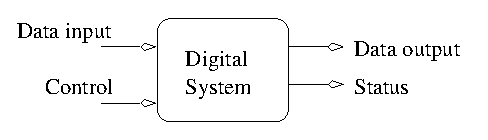
\includegraphics{./Fig4/Asys}}
\caption{A modified diagram of a digital system showing the classification
of the inputs and outputs.}
\label{fig:Asys}
\end{figure}

Some basic building blocks of digital systems are introduced.  
While a wide variety of blocks can be considered, those
proven to be most useful in the construction 
of digital circuits are presented.  If the right block for a particular
task does not exist, create a new block using the methods presented 
in the last chapter.  First in the examination of basic building 
blocks is a device that routes one bit of data to one of several
outputs based on an address.

\section{Decoder}
\index{decoder|(}
\begin{tabular}{|l|p{3.5in}|} \hline
Nomenclature:  & N:M decoder				\\ \hline
Data Input:    & 1-bit D		\\ \hline
Data Output:   & M-bit vector $y = y_{M-1} \ldots y_1 y_0$	\\ \hline
Control:       & N-bit vector $s = s_{N-1} \ldots s_1 s_0$	\\ \hline
Status:        & none					\\ \hline
Behavior:      & $y_s = D$ all other outputs equal 0	\\ \hline
\end{tabular}
\label{page:dec}
\\ \\
To understand this definition, examine an
instance of a 3:8 decoder shown at left in Figure~\ref{fig:3:8}.
Normally, the arrows indicating the direction of the information 
flow in to and out from the decoder are not drawn.  
To understand the behavior of the decoder, its
truth table is shown to the right of Figure~\ref{fig:3:8}. 
Due to space constraints, only part of the entire truth
table is shown.

\begin{figure}[ht]
\begin{tabular}[b]{p{1.0in}p{0.5in}l}
\includegraphics[0mm,20mm][12mm,12mm]{./Fig4/3:8.eps} & &
$\begin{array}{c|c|c|c||c|c|c}
s_2 & s_1 & s_0 & D & y_0 & y_1 & y_2\\ \hline
0 & 0 & 0 & 0 	& 0  &   0 &   0\\ \hline
0 & 0 & 0 & 1 	& 1  &   0 &   0\\ \hline
0 & 0 & 1 & 0 	& 0  &   0 &   0\\ \hline
0 & 0 & 1 & 1 	& 0  &   1 &   0\\ \hline
0 & 1 & 0 & 0 	& 0  &   0 &   0\\ \hline
0 & 1 & 0 & 1 	& 0  &   0 &   1\\ \hline
0 & 1 & 1 & 0 	& 0  &   0 &   0\\ \hline
0 & 1 & 1 & 1 	& 0  &   0 &   0\\ \hline
1 & 0 & 0 & 0 	& 0  &   0 &   0\\ \hline
1 & 0 & 0 & 1 	& 0  &   0 &   0\\
\end{array}$ \\
\end{tabular}
\caption{A 3:8 decoder (left) and part of its truth table (right).}
\label{fig:3:8}
\end{figure}

From the behavior listed in the description of the decoder, 
see that the $i^{th}$ output equals the data input, where
$i$ is the binary code of the select inputs.  In other
words, when $S=s_2 s_1 s_0 = 011_2 = 3_{10}$ and $D=1$,
then $y_7 y_6 y_5 y_4 y_3 y_2 y_1 y_0 = 00001000$.  If 
$S= s_2 s_1 s_0 = 011_2 = 3_{10}$ and $D=0$, then
$y_7 y_6 y_5 y_4 y_3 y_2 y_1 y_0 = 00000000$.   

The utility of this second case might be questionable because
all the outputs are the same and consequently one cannot
``see" where the output is being routed.  The resolution
to this dilemma requires considering the outputs 
through time.  A decoder is a box which sends a ``stream" of 
bits to some destination determined by the select lines.
If the destination knows that it is receiving the stream, then it
will be expecting both 1s and 0s through time.

The internal organization of a 3:8 decoder must process its four bits
of input, consisting of a 3-bit select and a 1-bit data input, and
eight bits of outputs.  In 
the previous chapter, each bit of the output could
be solved independently of the others. Hence, let's examine the $y_0$
output first.  Examination of the truth table and the behavior of
the decoder shows $y_0$ only equals 1 when
$(s_2, s_1, s_0) = (0, 0, 0)$ and $D=1$.  Borrowing the minterm
trick from page~\pageref{page:MinTrick}, $y_0=s_2's_1's_0'D$ results.
Every other output shares the characteristic that its output is
equal to 1 for a single input. Thus, each output is represented
by a minterm as shown in Figure~\ref{fig:3:8Guts}.

\begin{figure}[ht]
%% scalebox
\center{\scalebox{0.5}{\includegraphics{./Fig4/3:8Guts}}}
\caption{The internal organization of a 3:8 decoder.}
\label{fig:3:8Guts}
\end{figure}

In some digital applications, the need arises to build a larger decoder
from multiple smaller decoders.  This is done by fanning-out the data input
in a tree-like structure.  The following 4:16 decoder shows how a larger decoder is
built from several smaller 2:4 decoders. 

In order to accommodate the 16 outputs, four 2:4 decoders are stacked
on top of one another as shown in Figure~\ref{fig:BigDecoder}.  These
four 2:4 decoders have a total of four bits of input.  These four bits
are sourced by the output of a single 2:4 decoder.  The
single data input of this decoder is the input of the overall 4:16
decoder.  

\begin{figure}[ht]
\center{\scalebox{0.7}{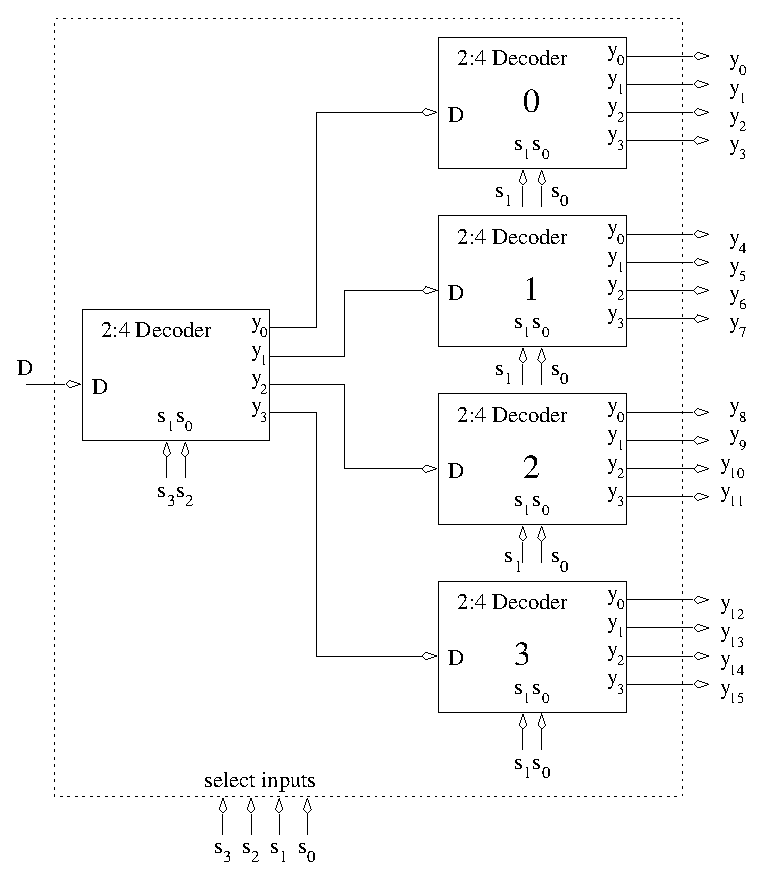
\includegraphics{./Fig4/BigDecoder}}}
\caption{A 4:16 decoder built from 2:4 decoders.} 
\label{fig:BigDecoder}
\end{figure}

Having organized the structure of the 2:4 decoders, all that remains 
is to route the select lines.  The outputs of the decoder labeled 
{\bf 3} in Figure~\ref{fig:BigDecoder} corresponds to outputs 
$y_{15} y_{14} y_{13} y_{12}$ 
of the 4:16 decoder.  Each of these outputs requires four bits of 
select with the form $s_3 s_2 s_1 s_0 = 11xx$.  Hence, $s_3 s_2 = 11$ 
must route the data input, $D$, to decoder {\bf 3}.  Hence, $s_3 s_2$ 
must be the select to the first level decoder in 
Figure~\ref{fig:BigDecoder}.   A similar argument for the 2:4 decoders 
labeled {\bf 0,1,2} reinforces the fact that $s_3 s_2$ must be the select 
to the first level decoder.  

Data routed to output $y_{12}$ has $s_3 s_2 s_1 s_0 = 1100$.  Thus, routing
at the second level of 2:4 decoders seems to be controlled by $s_1 s_0$.
Examining all the other outputs reinforces this assumption for all
the outputs.
\index{decoder|)}


\section{Multiplexer}
A multiplexer, often referred to as a mux, is data routing device 
which behaves exactly opposite of a decoder.  Its structure and
behavior is defined in the following table.
\\ \\
\index{multiplexer|(}
\begin{tabular}{|l|p{3.5in}|} \hline
Nomenclature:  & N:1 multiplexer                        \\ \hline
Data Input:    & M-bit vector $y=y_{M-1} \ldots y_1 y_0$    \\ \hline
Data Output:   & 1-bit F          \\ \hline
Control:       & $log_2(N)$-bit vector $s = s_{log_2(N)} \ldots s_1 s_0$	\\ \hline
Status:        & none                                   \\ \hline
Behavior:      & $F = y_s$				\\ \hline
\end{tabular}
\label{page:mux}
\\ \\
To understand this definition, examine an
instance of an 8:1 mux shown on the left in Figure~\ref{fig:8:1}.
From the behavior listed in the description of the multiplexer, 
the $i^{th}$ data input is routed to the data
output where the binary code of the select inputs is $i$.
For example, if $S=s_2 s_1 s_0 = 101_2 = 5_{10}$  and 
$y_7 y_6 y_5 y_4 y_3 y_2 y_1 y_0 = 00100000$, then
$F=1$.
\\ \\
\begin{figure}[ht]
\begin{tabular}{p{1.5in}p{0.5in}l}
\includegraphics[0mm,20mm][12mm,12mm]{./Fig4/8:1.eps} & &
$\begin{array}{c|c|c||c}
s_2 & s_1 & s_0 & F \\ \hline
0 & 0 & 0 & y_0 \\ \hline
0 & 0 & 1 & y_1 \\ \hline
0 & 1 & 0 & y_2 \\ \hline
0 & 1 & 1 & y_3 \\ \hline
1 & 0 & 0 & y_4 \\ \hline
1 & 0 & 1 & y_5 \\ \hline
1 & 1 & 0 & y_6 \\ \hline
1 & 1 & 1 & y_7 \\
\end{array}$
\end{tabular}
\caption{An 8:1 mux (left) and its truth table (right).}
\label{fig:8:1}
\end{figure}

The unusual form of the truth table shown in Figure~\ref{fig:8:1}
results from the fact that an 8:1 mux has a total of 11 
inputs.  There are a total of $2^{11}$ rows in this truth table
making it infeasible to list every combination of the inputs.
Consequently, in order to build an 8:1 mux, the structure of the truth table 
must be determined without
listing every combination of inputs.  Observe the $y_0$ input is routed 
to the output when 
$s_2 s_1 s_0 = 000$.  Consequently, $F=s_2' s_1' s_0' y_0$
for this input.  Each of the other outputs has a similar
minterm form.  Since only one of these ``minterms" can equal
1 for a particular select input, the minterms are ORed
together to form the output. The resulting internal 
organization of an 8:1 mux is shown in Figure~\ref{fig:8:1Guts}.

\begin{figure}[ht]
%% scalebox
\center{\scalebox{0.5}{\includegraphics{./Fig4/8:1Guts}}}
\caption{The internal organization of an 8:1 mux.}
\label{fig:8:1Guts}
\end{figure}

As with decoders, situations arise when a larger
mux is built from smaller muxes.  The key idea is to funnel down the many data 
inputs from smaller muxes to a single output.  For example, construct 
a 16:1 mux from several 4:1 muxes.  

In order to accommodate the 16 inputs, four 4:1 muxes are stacked
on top of one another as shown in Figure~\ref{fig:BigMux}.  These
four 4:1 muxes have a total of four bits of output.  These four bits
can nicely be routed by the inputs of a single 4:1 mux.  The
single data output of this mux is the input of the overall 16:1 mux.

\begin{figure}[ht]
\center{\scalebox{0.7}{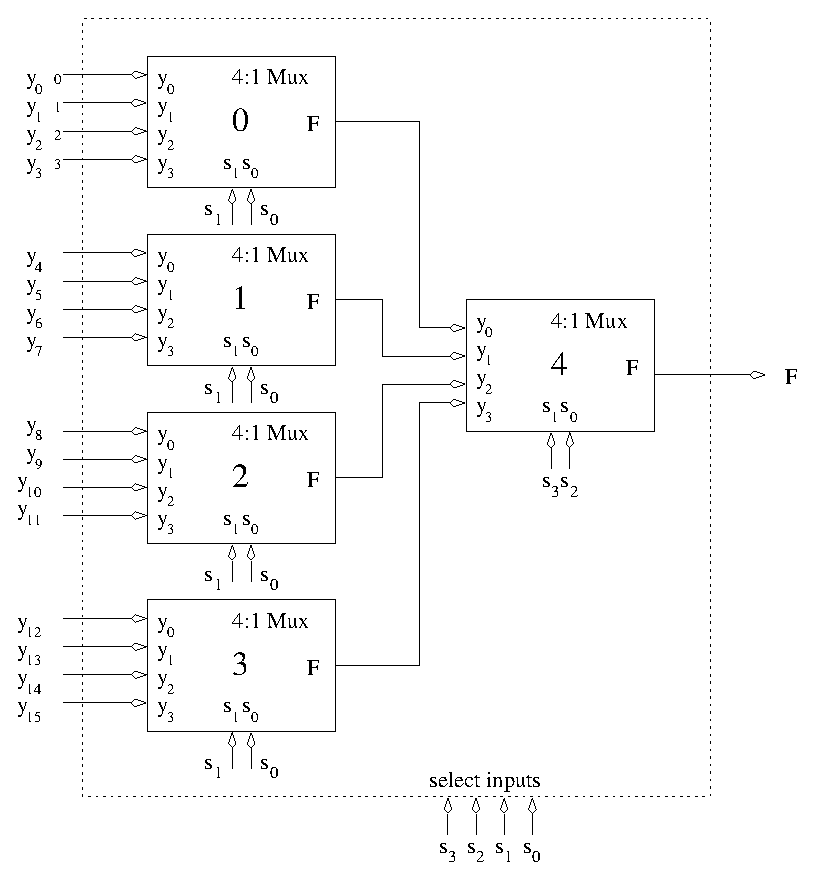
\includegraphics{./Fig4/BigMux.eps}}}
\caption{The construction of a 16:1 mux from 4:1 muxes.}
\label{fig:BigMux}
\end{figure}

The select lines are assigned to the 4:1 muxes based on the following 
argument.  The inputs of the mux labeled {\bf 3} in
Figure~\ref{fig:BigMux} corresponds to inputs $y_{15} y_{14} y_{13} y_{12}$ 
of the 16:1 mux.  Each of these inputs requires four bits of 
select with the form $s_3 s_2 s_1 s_0 = 11xx$.  Hence, $s_3 s_2 = 11$ 
must be the select for the output mux {\bf 4}.  
A similar argument for the 4:1
muxes labeled {\bf 0,1,2} reinforces the fact that $s_3 s_2$ must be 
the select to the output mux.

In order to route $y_{12}$ to the output, the select must equal
$s_3 s_2 s_1 s_0 = 1100$.  Thus, routing at the input level of 4:1 
muxes is controlled by $s_1 s_0$.  Examining all the other 
inputs reinforces this assumption.

Occasionally the need arises to construct a mux to handle
``wide" data inputs, that is data inputs which consist of more than
a single bit.  A mux that can handle many bits is referred to 
as a {\it multibit mux}.  \label{multibit mux} A M-bit N:1 mux is 
defined as a N:1 mux whose data inputs and data outputs are M-bits
wide.  For example, the 4-bit 2:1 mux shown in Figure~\ref{fig:4x2x1mux} 
has two data inputs and one data output each 4-bits wide.  The internal
organization of this mux is shown on the right-hand side of 
Figure~\ref{fig:4x2x1mux}.  Four, 2:1 muxes are needed to 
accommodate all the data.  Since the data inputs are to 
be handled as a single whole, they must be routed to the
same input on each of the 2:1 muxes.
\label{page:wmu}

\begin{figure}[ht]
%% scalebox
\center{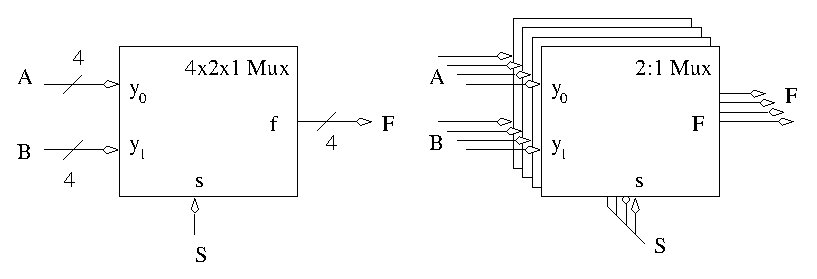
\includegraphics{./Fig4/4x2x1mux}}
\caption{The organization of a 4-bit 2:1 mux.  The slash labeled ``4" 
denotes the fact that these signals are 4-bits wide.}
\label{fig:4x2x1mux}
\end{figure}
\index{multiplexer|)}


\section{The Adder}
An N-bit adder is a circuit which adds two N-bit binary numbers 
$A,B$ together generating an N-bit sum $S$ and an overflow 
indication, Ovf.   

\index{adder|(}
\begin{tabular}{|l|p{3.5in}|} \hline                    
Nomenclature:  & N-bit adder				\\ \hline
Data Input:    & two N-bit vectors $A$ and $B$		\\ \hline
Data Output:   & N-bit vector sum			\\ \hline
Control:       & none					\\ \hline
Status:        & 1-bit ovf 				\\ \hline
Behavior:      & $sum = A+B$				\\ \hline
\end{tabular}
\\ \\
The behavior of the adder is exactly as expected after reading
page~\pageref{page:addition}.  Furthermore, the overflow output is asserted 
when the adder output is greater than or equal to $2^N$.  The construction 
of an adder illustrates an approach that can be utilized for circuits 
whose function can be broken down into modular pieces. 

Approaching the design of a 4-bit adder ($N=4$) using the design 
philosophy introduced in Chapter 2, the truth table has eight bits
of inputs, 256 rows, and nine bits of outputs.  The task would be tedious,
error-prone, producing a realization with a large number of 
gates.  Instead of building the circuit as one monolithic piece, a module 
is designed that adds one set of bits together.  Four of these modules are
then connected in series to add four bits together.
For example, in Figure~\ref{fig:add} $A=1011$ and $B=0001$ are added
together using the approach of page~\pageref{page:addition}.

\begin{figure}[ht]
\center{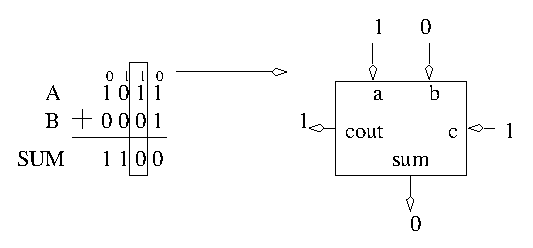
\includegraphics{./Fig4/add}}
\caption{An addition problem and the values of one of its
bit slices placed on a full adder.}
\label{fig:add}
\end{figure}

This addition problem contains four {\it bit-slices} \index{bit-slice}.
Each bit-slice adds one bit's worth of the overall addition problem.  
The addition circuit is then constructed by stringing together four
of these bit-slice adders (called full-adders).  In the example shown
in Figure~\ref{fig:add}, the second bit-slice of the addition problem 
is outlined.  The inputs and outputs of this bit-slice are placed on 
a full adder.  The full adder has three bits of input and two bits of output.
To build a 4-bit adder, four full adders are strung together in series
using the carry lines.  The truth table for the full adder is created 
by enumerating every combination of inputs and determining the sum and 
carry-out for each.  The carry-out and sum together are the 2-bit sum
created by adding together the three input bits.

\begin{tabular}{lp{0.5in}l}
$\begin{array}{c|c|c||c|c}
a & b & c & cout & sum \\ \hline
0 & 0 & 0 & 0 & 0 \\ \hline
0 & 0 & 1 & 0 & 1 \\ \hline
0 & 1 & 0 & 0 & 1 \\ \hline
0 & 1 & 1 & 1 & 0 \\ \hline
1 & 0 & 0 & 0 & 1 \\ \hline
1 & 0 & 1 & 1 & 0 \\ \hline
1 & 1 & 0 & 1 & 0 \\ \hline
1 & 1 & 1 & 1 & 1 \\
\end{array}$
			&
{\footnotesize
\begin{tabular}{ll}
$ \begin{array} {c||c|c|c|c}
        a \bs bc & 00 & 01 & 11 & 10 \\ \hline \hline
        0          &    &    & 1  &    \\ \hline
        1          &    & 1  & 1  & 1  \\
\end{array}$					&
$ \begin{array} {c||c|c|c|c}
        a \bs bcin & 00 & 01 & 11 & 10 \\ \hline \hline
        0          &    & 1  &    & 1  \\ \hline
        1          & 1  &    & 1  &    \\
\end{array}$ 					\\
cout = bc + a b + ac				&
sum=a b' c' + a'b'c + abc + a'bc'		\\
\end{tabular}	}
\end{tabular}


The \SOPmin expression for the outputs is arrived at by
solving Kmaps for each of the outputs.  Once, the internal
organization of a full adder is complete, four of them
are connected together as shown in Figure~\ref{fig:adder}
to build a 4-bit adder.

\begin{figure}[ht]
\center{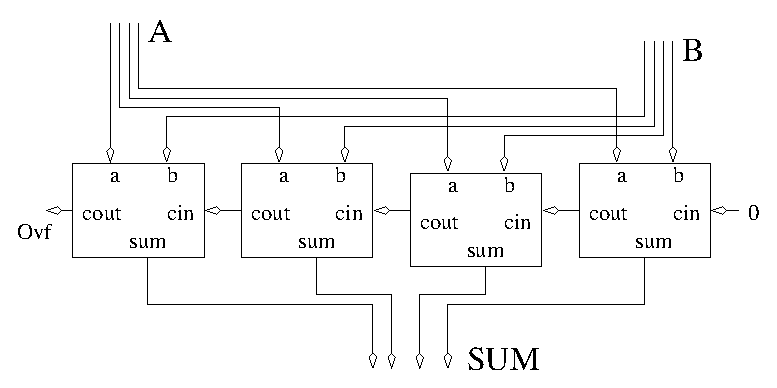
\includegraphics{./Fig4/adder}}
\caption{The arrangement of full adders to create a multi-bit
adder.}
\label{fig:adder}
\end{figure}
\label{page:add}

The carry-out of each bit-slice becomes the carry-in of the
next, more significant, full adder.  This sequence is necessarily
broken at the beginning and end of the chain of full 
adders.  Since there is no carry-in to the least significant
bit of an addition problem, the carry-in to the least significant
full adder is set to 0.  Since overflow occurs when the result 
of the addition process requires more bits than the word size, a 
carry-out from the most significant full adder indicates overflow.
\index{adder|)}

\section{The Adder Subtractor}
\index{adder subtractor|(}
As its name implies, an adder subtractor can perform two separate
functions.  From a black-box perspective, the only difference between
this module and an adder is the presence of a control input to select
which function the adder subtractor performs.
 

\begin{tabular}{|l|p{3.5in}|} \hline
Nomenclature:  & N-bit adder subtractor                 \\ \hline
Data Input:    & two N-bit vectors $A$ and $B$           \\ \hline  
Data Output:   & N-bit vector  $s$               \\ \hline
Control:       & 1-bit $f$                     \\ \hline
Status:        & 1-bit ovf 				\\ \hline
Behavior:      & if c=0 then $s = A+B$ else $s=A-B$     \\ \hline
\end{tabular}
\\ \\
For now, assume the inputs and output of an adder subtractor are
2's-complement numbers.  Addition of 2's-complement numbers proceeds 
like the addition of regular binary numbers.  For now, 
ignore overflow conditions.  The subtraction process
for 2's-complement numbers, described on page~\pageref{page:2sub}, rewrites
the subtraction problem $A-B$ as an addition problem $A+(-B)$.  The caveat
is that $B$ must be negated.  Since both the addition and the subtraction 
problem
require an adder, all that is required is to pass either $B$ or $-B$ to the
adder depending on which operation is to be performed.  This idea is
presented in Figure~\ref{fig:AddSub}.

\begin{figure}[ht]
\center{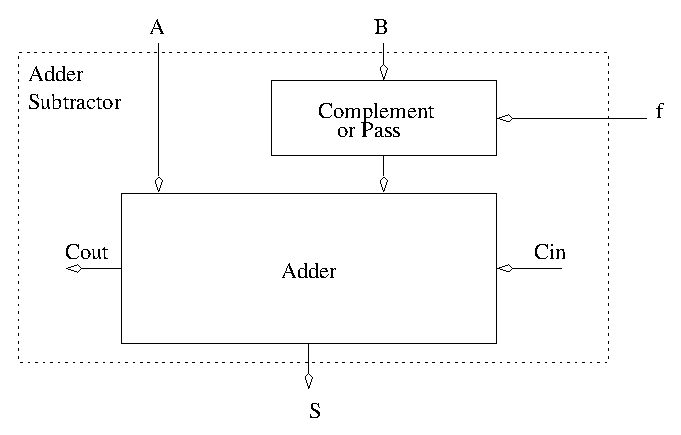
\includegraphics{./Fig4/AddSub}}
\caption{The idea behind the creation of an adder subtractor circuit.}
\label{fig:AddSub}
\end{figure}

The ``Complement or Pass" box in Figure~\ref{fig:AddSub} produces 
either $B$ when $f=0$ (addition) or $-B$ when $f=1$ (subtraction).
The process of complementing $B$ is to flip the bits and to add 1.
To avoid adding a second adder to perform the ``add 1" 
operation the adder shown in Figure~\ref{fig:AddSub} performs 
both $A+B$ and the ``add 1".  This little piece of magic is 
accomplished by hijacking the carry-in to the least significant 
bit of the full adder chain shown Figure~\ref{fig:adder}.  Instead
of hardwiring $cin$ shown in Figure~\ref{fig:AddSub} to 0, $cin$ is 
connected to $f$.  
When $f=1$, an extra 1 will be added to sum. The 2's-complement of
$B$ is computed in two separate steps: The ``Complement or Pass" box 
negates the bits of $B$ (when $f=1$) and the adder adds 1
(when $f=1$). Hence, the circuit performs a subtraction when $f=1$.
When $f=0$, the ``Complement or Pass" box will pass through $B$
unchanged, the adder does not add anything extra to the inputs and,
consequently, the circuit performs $A+B$.

The ``Complement or Pass" box is broken down into bit-slices, each
bit of $B$ is sent to its own slice along with the $f$ control
bit.  If $f=0$, then the slice outputs the input $B$ bit.  If $f=1$, 
then the slice outputs the complement of the $B$ bit.
The truth table is shown below.

$$\begin{array}{c|c||c}
b & f & out \\ \hline
0 & 0 & 0 \\ \hline
0 & 1 & 1 \\ \hline
1 & 0 & 1 \\ \hline
1 & 1 & 0 \\
\end{array}$$

Solving the truth table yields $out = b'f + bf' = b \oplus f$.
Each of these bit-slices is organized along with the components
in Figure~\ref{fig:AddSub} yielding the circuit diagram in
Figure~\ref{fig:TotalAddSub}.


\begin{figure}[ht]
\center{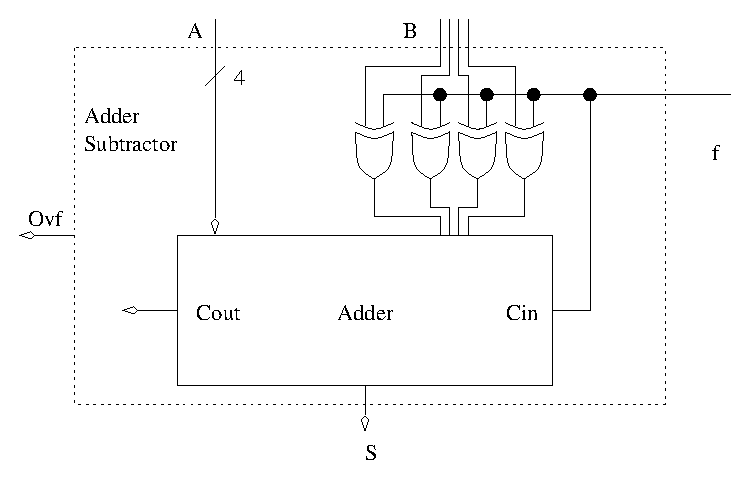
\includegraphics{./Fig4/TotalAddSub}}
\caption{The construction of 4-bit adder subtractor.}
\label{fig:TotalAddSub}
\end{figure}
\label{page:as}


According to page~\pageref{page:Ovf}, overflow in a 2's-complement 
operation occurs when the carry-in and carry-out to the most
significant bit-slice of the addition disagree.  In order to 
build a circuit to check this condition, the ``Adder" box shown in 
Figure~\ref{fig:TotalAddSub} must be opened revealing
the chain of full adders as shown in Figure~\ref{fig:AddSub}.
The derivation of the truth table and the circuit realization
is left as an exercise at the end of the chapter.
\index{adder subtractor|)}

\section{The Comparator}
A comparator is a device which determines the relative magnitude
of its two inputs.

\index{comparator|(}
\begin{tabular}{|l|p{3.5in}|} \hline
Nomenclature:  & N-bit comparator                \\ \hline
Data Input:    & two N-bit vectors $X$ and $Y$           \\ \hline  
Data Output:   & none               \\ \hline
Control:       & none                      \\ \hline
Status:        & 1-bit $G,L,E$ \\ \hline
Behavior:      & 
		$$\begin{array}{l|l|l|l}
      			cond  & E & L & G \\ \hline
			X = Y & 1 & 0 & 0 \\ \hline
			X < Y & 0 & 1 & 0 \\ \hline
			X > Y & 0 & 0 & 1 \\
		\end{array}$$			\\ \hline
\end{tabular}
\label{page:com}
\index{comparator!truth table}

Comparators are rather unique because they lack data output.  That is
not to say, comparators do not have any output. Rather, their status outputs are quite
useful.  The comparator examines its two $N$-bit inputs, denoted $X$ and
$Y$, and outputs three bits describing their relative magnitudes.  
Each of these three bits, $E,L,G$, is asserted when $X$ equals $Y$, 
$X$ is less than $Y$, or $X$ is greater than $Y$, respectively.  

Much like the adder circuit the truth table method is not very 
useful for designing large comparators.  For example, a 16-bit 
comparator has two 16-bit inputs, or 32 bits of inputs, for an 
astounding $2^{32}$ rows in the truth table.  

The construction of large comparators is based on the method that 
employed to determine the relative magnitude of two numbers $X$
and $Y$, working from the most to least significant
bits.  At each step, compare a bit of $X$ and $Y$.  If the bits
are equal, then continue to the next least significant bit.  Otherwise,
either $X$ or $Y$ is larger, and the comparison is over.

Large comparators are constructed by stringing together a series
of modified 1-bit comparators as shown in Figure~\ref{fig:Compare}.  
Each bit-slice has as input a pair 
of bits from $X$ and $Y$, and $Ein$, $Gin$ and $Lin$ signals from a
more significant bit-slice.  $Ein$, $Lin$ and $Gin$ tell a bit-slice the 
status of the magnitude of $X$ and $Y$ in the bit positions to
its left.  Each bit-slice has three bits of output, $Eout$, $Lout$, and 
$Gout$, communicating the relative magnitude of the inputs so far.

\begin{figure}[ht]
\center{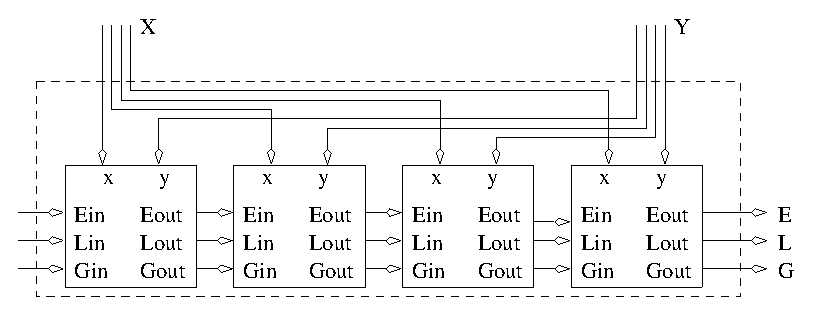
\includegraphics{./Fig4/Compare}}
\caption{The arrangement of the bit-slices for the comparator.}
\label{fig:Compare}
\end{figure}

The truth table for a bit-slice of the comparator has five inputs, 
$x, y, Ein, Lin$ and $Gin$.  Each bit-slice has three outputs, 
$Eout, Lout$ and $Gout$.  A portion of the truth table is shown below.

$$\begin{array}{c|c|c|c|c||c|c|c}
x & y & Ein & Lin & Gin & Eout & Lout & Gout	\\ \hline
0 & 0 & 0   & 0   & 0 	& x    & x    & x	\\ \hline
0 & 0 & 0   & 0   & 1 	& 0    & 0    & 1	\\ \hline
0 & 0 & 0   & 1   & 0 	& 0    & 1    & 0	\\ \hline
0 & 0 & 0   & 1   & 1 	& x    & x    & x	\\ \hline
0 & 0 & 1   & 0   & 0 	& 1    & 0    & 0	\\
\end{array}$$

With five bits of input, the truth table has a total of 32 rows, only
five of which are shown above.  Two rows have their outputs set to 
``don't cares" because they represent impossible situations.  The inputs
in the first row, state that the two numbers have no relative 
magnitude relative to one another.  The inputs on the fourth row 
claim that $X<Y$ and $X>Y$ simultaneously, an impossible situation.
The second row states that it has already been determined that $X>Y$,
so it does not matter what $x$ and $y$ are because their value cannot 
effect a decision that has occurred
in a more significant bit-slice.  Similarly, the third row states
that $X<Y$, so the outputs just propagate this fact, regardless 
of $x$ and $y$, because the bits of this slice are less significant
than those which decided $X<Y$.  The fifth row states that
so far $X=Y$ and since the bit-slice inputs are equal, the 
two inputs are still equal.  The remainder of the truth table will
be completed in an exercise at the end of the chapter.

The final question that must be answered is ``What should $Ein$, $Lin$,
and $Gin$, on the far left of the Figure~\ref{fig:Compare}, be assigned?"
The answer is that the $Ein, Lin,Gin$ inputs to the most significant bit-slice
should be set to 1,0,0 because $X$ and $Y$ are initially assumed to be equal.
From the preceding paragraph, observe that whenever it is determined
that $X>Y$ or $X<Y$, the comparator bit-slices will not change this 
fact.  Hence, starting the circuit off from any other initial condition
would cause an irreversible bias.  Another way to view this situation
is to realize that any binary number can be considered to have an infinite 
number of leading 0s, all of which are equal.
\index{comparator|)}

\section{Three-State Buffer}
\index{three-state buffer|(}
\begin{tabular}{|l|p{3.5in}|} \hline
Nomenclature:  & Three-state buffer	\\ \hline
Data Input:    & 1-bit X		\\ \hline
Data Output:   & 1-bit Y		\\ \hline
Control:       & 1-bit $c$              \\ \hline
Status:        & none			\\ \hline
Others:        & none			\\ \hline
Behavior:      & The output equals the input when 
		$C=1$ otherwise the output is 
		disconnected from input. \\ \hline                                                                               
\end{tabular}
\label{page:tsb}
\\ \\
When several devices share a common signaling pathway, as with
a data bus, it is important for every device to be capable of 
asserting data onto the bus, but only one device at a time
actually asserts data.  This effect can only be accomplished if each
device is capable of electrically disconnecting itself from the
bus.  The three-state buffer shown in Figure~\ref{fig:tsb} does
this under the control of the $c$ signal.
                                                                                
\begin{figure}[ht]
\begin{tabular}[b]{p{1.0in}p{0.5in}l}
\includegraphics[10mm,10mm][12mm,12mm]{./Fig4/tsb} & &
                                                                                
$\begin{array}{c|c||c}
X & C & Y \\ \hline
x & 0 & Z \\ \hline
0 & 1 & 0 \\ \hline
1 & 1 & 1 \\
\end{array}$
\end{tabular}
\caption{The symbol and truth table for a three-state buffer.}
\label{fig:tsb}
\end{figure}

Notice, when $C=1$, then $Y=X$; the output equals the
input.  But, when $C=0$, the output equals $Z$.  $Z$ is
a symbol commonly used in electrical engineering
to refer to impedance (reciprocal of resistance).  The
$Z$ means the output is not connected to anything.

It is common to see $N$ three-state buffers organized together to
produce an N-bit three-state buffer.  In such an arrangement, 
each bit of input is routed to its own three-state buffer,
and the control input is routed to all of the three-state 
buffers.  Each three-state buffer contributes its one bit 
of output to the overall output from the N-bit three-state
buffer.
 

Directly connecting together outputs of two gates creates
a situation where the two gates may produce different outputs
resulting in a short circuit.  This connection will
eventually lead to the failure of one or both of the gates.
Clearly, a system should not be designed with such a flaw.
However, cases arise when it makes sense to want to wire
together the outputs of several gates.

The bus \index{bus} in a computer is a collection
of related signals that move information between any pair
of devices on the bus.  Allowing a bus to be used by many
different devices increases its utilization at the expense 
of increased complexity.  Look at the example bus in 
Figure~\ref{fig:bus} which connects a CPU, RAM, and Disk.
Each of these devices may want data to be sent or
received from any of the others.  The shaded box in each device 
(CPU, RAM, Disk) is called out on the right side of Figure~\ref{fig:bus}.
The input register latches data from the bus and the output
register holds the data to be asserted on the bus.  The 
three-state buffer can disconnect the output register from the bus 
allowing one of the other devices to assert data on the bus.  
It is important, and fairly obvious, that only one device at a 
time can assert data on the bus.  

\begin{figure}[ht]
\center{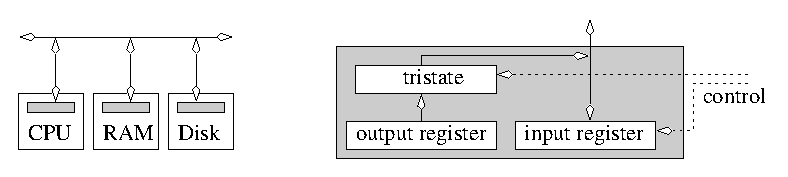
\includegraphics{./Fig4/bus}}
\caption{Three devices on a bus.  The internal circuitry in
each device to make it work.}
\label{fig:bus}
\end{figure}
\index{three-state buffer|)}

\section{Wire Logic}
\index{wire logic|(}
When  designing a digital system which contains a device
such as an adder which manipulates a pair of N-bit inputs representing
binary numbers, it is easy to forget that those N bits are really
N separate wires being grouped together.  As a
digital designer, one has access to each of these wires
and can manipulate them as necessary.  This point is important
to remember when designing with the basic building
blocks in this chapter because the number of bits representing a 
value must match the size of the device input.  For example, 
a 4-bit value cannot be run into an 8-bit-wide input and 
expected to work without some consideration of how to
handle the four, remaining bit positions.

For example, assume a 4-bit binary number 
needs to be added to an 8-bit number.  In order to 
accommodate the 8-bit number, an 8-bit
adder needs to be used.  Unfortunately, this decision creates a 
problem with the 
4-bit operand because the upper four bits of its input
are unoccupied.  The solution is to fill in the upper
four bits with 0s.  This solution is called padding with 0s 
because just like when padding is placed around an item
being shipped in a container to prevent it 
from moving around, padding a binary number with 0s 
keeps it aligned in its word-sized container. Further, the padding operation does not 
change the value of the 4-bit number.

Padding a 2's-complement number, a process called sign-extension,
is slightly more complex. Consider the problem of adding or 
subtracting a 4-bit 2's-complement number to an 8-bit 2's-complement 
number using an 8-bit adder subtractor.  The important 
point to keep in mind is that the value of the original, 4-bit, 
2's-complement must be the same as the value of the sign-extended 
8-bit 2's-complement value.  If the 4-bit value were 1111, 
representing -1 in decimal, then padding the upper four
bits with 0s would yield 00001111, which represents +15
in 8-bit 2's-complement.  This approach is not the correct way to proceed
because the original value of -1 was converted into +15 
through the sign-extension process.  Instead, the value should have been padded 
with 1s yielding 11111111, which represents -1 in an
8-bit 2's-complement number.  To show
that any negative 4-bit value padded with 1s retains its value,
show that the values of original and sign-extended 
numbers are the same when the bits are flipped and 1 is added.
Further,  any positive 4-bit value should
be padded with 0s to retain its value.  In general, the 4-bit
value needs to be padded with four copies of the most significant 
bit.

When representing a decimal value, using the base-10 numbering system, 
multiplication of a 
number by 10 can be accomplished by moving all the digits
one position to the left and inserting a 0 in the vacated
digit position.  With binary-represented values,
multiplication by 2 can be accomplished by moving all the
bits one position to the left and inserting a 0 in the 
vacated position.  This manipulation can be handled by padding the least
significant bit position with a 0.

Another useful manipulation is to combine signals together.  For 
example, consider a pair of 4-bit binary numbers
are to be added together, and their 5-bit sum is to be reported.
One alternative might be to pad each of the 4-bit inputs with a 0 and 
pass them along to a 5-bit adder.  Alternatively, 
the numbers could be used unmodified as inputs to a 4-bit adder, 
and combine the overflow output
of the 4-bit adder to the 4-bit sum output, producing a 5-bit result.
Though unconventional, this manipulation is perfectly legal and perfectly 
correct because, the overflow signal is just the 
carry-out from the most significant full adder.

\index{wire logic|)}

\section{Combinations}
The devices introduced in this section have limited utility when
used by themselves. Their real potential is realized when combined together. 
When connecting two components, the data 
outputs of one device are typically connected to the data inputs 
of other.  Likewise, the status outputs are typically connected 
to control inputs of another device.  But how are the components arranged? 
A useful starting point is to phrase the solution 
of the design problem in terms of a simple algorithm.  Algorithms 
are composed of statements. The algorithms to be constructed 
have several different types of statements.

\subsection{Arithmetic Statements}
Arithmetic statements perform the data manipulations required by
design problems.  An arithmetic statement consists of two parts,
a left-hand side (LHS) and a right-hand side (RHS), related to one
another by an equal sign.  The RHS describes the operation and its
inputs, while the LHS represents the variable denoting the output 
of the arithmetic operation.  For example, the following line of
code describes the addition of two values.

\begin{verbatim}
    x = y + 3
\end{verbatim}

The hardware realization of this line of code is an adder with \verb+y+ 
and 3 as inputs and \verb+x+ as its output.  The algorithm does not
specify the width of the \verb+x+ and \verb+y+ signals. These must
be determined from accompanying information.


\subsection{Conditional Statements}
Conditional statements arise in programming languages in the
form of \verb+if/then/else+ statements.  All conditional statements consist 
of three parts, the condition to be checked (the \verb+if+ clause), the 
statement to be evaluated when the condition is true (the \verb+then+ clause), 
and the statement to be evaluated when the condition is false (the
\verb+else+ clause).

Typically, the condition being evaluated seeks the relative
magnitude of two binary numbers.  For example, consider checking whether
 \verb+(a<4)+.  This comparison can be
realized by routing \verb+a+ and \verb+4+ into the $x$ and
$y$ inputs of a comparator and using the $L$ output.

The consequence of the condition is to cause the evaluation either of
the \verb+then+ clause or of the \verb+else+ clause.  For now, these 
clauses will 
be arithmetic statements.  In order to illustrate the hardware
realization of a conditional statement, consider the following
example.

\begin{verbatim}
    if (a<4) then x=y+3 else x=y+7
\end{verbatim}

The solution to the conditional assignment statement utilizes 
a comparator to determine the relative magnitudes of \verb+a+ 
and \verb+4+.  It is important to note in the solution shown in
Figure~\ref{fig:cond} which of the 
comparator's inputs is $x$ and $y$.  Of the three status outputs, 
the $L$ signal is used as the select on the multiplexer's inputs.  The 
other two comparator outputs should not be shown since they are
not used. 


\begin{figure}[ht]
\center{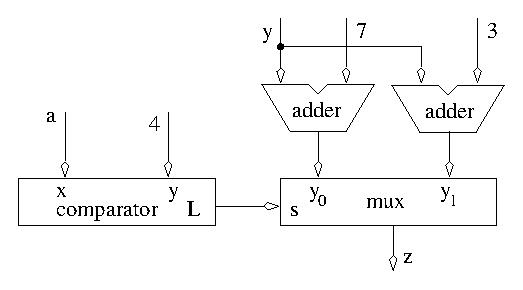
\includegraphics{./Fig4/cond}}
\caption{A combination of components to realize a conditional assignment
statement.}
\label{fig:cond}
\end{figure}

Each of the arithmetic operations in the algorithm is realized 
by its own adder. Notice in Figure~\ref{fig:cond} that both 
adders compute their values, and the job of the multiplexer is to 
select one of the adder outputs based on the results of the $L$ output 
from the comparator.    Since the LHS of both assignment statements
involved the same variable, the output of the mux is labeled with
$x$.  When \verb+a<4+, then 
$L=1$ and, consequently, the $y_1$ output of the mux is routed to the
output.  According to the algorithm, when \verb+a<4+, then $x=y+3$.
Consequently, $y+3$ should be routed to the $y_1$ input of the mux.
Now, only $y+7$ is left to be routed to the $y_0$ input of the mux.  It is
important to annotate the mux inputs with $y_1$ and $y_0$ in order
demonstrate that the solution works correctly.

The previous solution is more complex than it needs to be. An adder
can be removed from the circuit by noting that in the RHS of both 
assignments, the variable $y$ has either 3 or 7 added to it.  
Consequently, a mux can be used to switch through either a 3 or
7 and then to add this mux's output to $y$ as shown in 
Figure~\ref{fig:cond2}.

\begin{figure}[ht]
\center{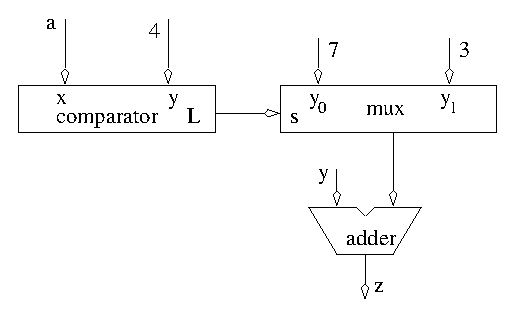
\includegraphics{./Fig4/cond2}}
\caption{A better realization of the conditional assignment statement.}
\label{fig:cond2}
\end{figure}

Make it a habit to identify ways to reduce the complexity
of a circuit whenever possible.  After all, one of the core
principles of engineering is always endeavor to do the most with 
the least.

\section{Exercises}
\section{Exercises}
\label{section:comboBbExercises}
\graphicspath{ {./chapter04/FigHw} }

\begin{enumerate}
    \item \textbf{ (2 pts. each)}Short answer:
        \begin{enumerate}
            \item How many 3:8 decoders would it take to build a 9:512 decoder?

                \begin{onlysolution} \textbf{Solutions} \itshape{A total of 73 decoders are required.  There
                        are 512/8 = 64 on
                    the output layer, 64/8 = 8 in the middle layer and 1 on the input.}
                \end{onlysolution}
            \item How many AND gates are there in a $2^N$:1 mux?

                \begin{onlysolution} \textbf{Solutions} \itshape{ Each input requires 1 AND gate, hence $2^N$
                    AND gates.}
                \end{onlysolution}
            \item How many AND gates are there in a $2^N:1$ mux which is
                constructed out of 2:1 muxes?

                \begin{onlysolution} \textbf{Solutions} \itshape{ A $2^N$ Mux requires the following number
                        of 2:1 muxes:
                        $$ 2^N/2 + 2^N/4 + ... + 2^N/2^N = $$
                        $$ 2^N(1/2 + 1/4 + ... + 1/2^N) = $$
                        $$ 2^N(1-1/2^(N+1)) =  $$
                        $$ 2^N - 1  $$
                        Since each 2:1 mux contains 2 AND gates, the total number of AND gates is
                        $2^(N+1) - 2$.
                    }
                \end{onlysolution}

            \item How many AND gates are there in a $2^N$:1 mux which is
                constructed out of $2^L$:1 muxes, assume that
                $2^N$ is an integer multiple of $2^L$?

                \begin{onlysolution} \textbf{Solutions} \itshape{
                        A $2^N$ Mux requires the following number of $2^L:1$ muxes:
                        $$ 2^N/2^L + 2^N/2^(2L) + ... 2^N/2^(kL) $$
                        $$ 2^N(1/2^L + 1/2^(2L) + ... 1/2^(kL)) $$
                        Where $k = N/L$.  Each $2^L:1$ mux requires $2^L$ AND gates for its construction,
                        so the number of AND gates is the product of the number of $2^L:1$ muxes and the
                        number of AND gates in a single $2^L:1$ mux, or:
                        $$ 2^N * 2^L(1/2^L + 1/2^(2L) + ... 1/2^(kL)) $$
                        $$ 2^N (1 + 1/2 + ... 1/2^k) $$
                        $$ 2^N (2-1/2^(k+1)) $$
                        $$ 2^N (2-1/2^(N/L+1) $$
                            $$ 2^(N+1) - 2^(N-N/L-1) $$
                        }
                    \end{onlysolution}

            \end{enumerate}

        \item \textbf{ (6 pts.)}Determine the \SOPmin expression for each of the
            three outputs of a bit-slice of the comparator.

            \begin{onlysolution} \textbf{Solutions} \itshape{
                    The following five variable Kmap describes $E_{out}$

                    \begin{tabular}{cc}
                        $
                        \begin{array} {c||c|c|c|c}
                            L_{in} G_{in}  \bs x  y & 00 & 01 & 11 & 10 \\ \hline \hline
                            00       & x  & x  & x  &  x \\ \hline
                            01       & 0  & 0  & 0  &  0 \\ \hline
                            11       & x  & x  & x  &  x \\ \hline
                            10       & 0  & 0  & 0  &  0 \\
                        \end{array}$
                        &
                        $
                        \begin{array} {c||c|c|c|c}
                            L_{in} G_{in}  \bs x  y & 00 & 01 & 11 & 10 \\ \hline \hline
                            00       & 1  & 0  & 1  & 0  \\ \hline
                            01       & x  & x  & x  & x  \\ \hline
                            11       & x  & x  & x  & x  \\ \hline
                            10       & x  & x  & x  & x  \\
                        \end{array}$  \\
                        $E_{in}=0$ & $E_{in}=1$ \\
                        \multicolumn{2}{c}{$E_{out} = L_{in}'G_{in}'x'y' + L_{in}'G_{in}'xy $} \\
                    \end{tabular}

                    The following five variable Kmap describes $G_{out}$

                    \begin{tabular}{cc}
                        $
                        \begin{array} {c||c|c|c|c}
                            L_{in} G_{in}  \bs x  y & 00 & 01 & 11 & 10 \\ \hline \hline
                            00       & x  & x  & x  & x  \\ \hline
                            01       & 1  & 1  & 1  & 1  \\ \hline
                            11       & x  & x  & x  & x  \\ \hline
                            10       & 0  & 0  & 0  & 0  \\
                        \end{array}$
                        &
                        $
                        \begin{array} {c||c|c|c|c}
                            L_{in} G_{in}  \bs x  y & 00 & 01 & 11 & 10 \\ \hline \hline
                            00       & 0  & 0  & 0  & 1  \\ \hline
                            01       & x  & x  & x  & x  \\ \hline
                            11       & x  & x  & x  & x  \\ \hline
                            10       & x  & x  & x  & x  \\
                        \end{array}$  \\
                        $E_{in}=0$ & $E_{in}=1$ \\
                        \multicolumn{2}{c}{$G_{out} = G_{in} + L_{in}'xy'$} \\
                    \end{tabular}

                    The following five variable Kmap describes $L_{out}$

                    \begin{tabular}{cc}
                        $
                        \begin{array} {c||c|c|c|c}
                            L_{in} G_{in}  \bs x  y & 00 & 01 & 11 & 10 \\ \hline \hline
                            00       & x  & x  & x  & x  \\ \hline
                            01       & 0  & 0  & 0  & 0  \\ \hline
                            11       & x  & x  & x  & x  \\ \hline
                            10       & 1  & 1  & 1  & 1  \\
                        \end{array}$
                        &
                        $
                        \begin{array} {c||c|c|c|c}
                            L_{in} G_{in}  \bs x  y & 00 & 01 & 11 & 10 \\ \hline \hline
                            00       & 0  & 1  & 0  & 0  \\ \hline
                            01       & x  & x  & x  & x  \\ \hline
                            11       & x  & x  & x  & x  \\ \hline
                            10       & x  & x  & x  & x  \\
                        \end{array}$  \\
                        $E_{in}=0$ & $E_{in}=1$ \\
                        \multicolumn{2}{c}{$L_{out} = L_{in} + G_{in}'x'y$} \\
                    \end{tabular}
                }
            \end{onlysolution}

        \item \textbf{ (2 pts.)}Show how to connect together four 4-bit comparators to
            construct a 16-bit comparator.

            \begin{onlysolution} \textbf{Solutions} \itshape{ Figure forthcoming}
            \end{onlysolution}

        \item \textbf{ (2 pts.)}Determine the circuitry for the overflow detection
            circuit for a 2's-complement adder subtractor.  See page~\pageref{page:Ovf}.

            \begin{onlysolution} \textbf{Solutions} \itshape{
                    $
                    \begin{array} {c||c|c} \\
                        c_{in}  \bs c_{out} & 0 & 1 \\ \hline
                        0    &   & 1 \\ \hline
                        1    & 1 &   \\
                    \end{array}$   \\
                    Thus $ovf = c_{in}' c_{out} + c_{in} c_{out}' =  c_{in} \oplus c_{out} $
                }
            \end{onlysolution}

        \item \textbf{ (10 pts.)}Build a BCD to 7-Segment Display converter using
            Espresso.

            \begin{buildingblock}{BCD to 7-segment}
                \index{bcd to 7-segment}
                \label{page:7seg}
                \begin{tabular}{|l|p{3.5in}|} \hline
                    Nomenclature:  & BCD to 7-segment converter                \\ \hline
                    Data Input:    & 4-bit vector $D=d_3 d_2 d_1 d_0$  \\ \hline
                    Data Output:   & 7-bit vector $Y=y_6 \ldots y_1 y_0$    \\ \hline
                    Control:       & none                                   \\ \hline
                    Status:        & none                                   \\ \hline
                    Behavior:      & The output drives a 7-segment display pattern
                    representing the BCD digit.  \\ \hline
                \end{tabular}
            \end{buildingblock}

            A binary coded digit (BCD) is a 4-bit binary number that is constrained
            to assume the values of 0-9. That is, 1010 ... 1111 are illegal BCD digits.

            A 7-segment display is a box with seven inputs and seven output LED bars.
            Each input is wired to an LED bar that is illuminated when a 1 is applied
            to its input.
            Each of the seven LED segments is numbered according to the pattern shown
            on the left-hand side of Figure~\ref{fig:BCD}.

            \begin{figure}[ht]
                \center{\scalebox{0.7}{\includegraphics{Prob4-5}}}
                \caption{The numbering of the segments in a 7-segment display.
                The patterns of the BCD digits.}
                \label{fig:BCD}
            \end{figure}

            The pattern of LEDs to illuminate for each BCD digit is shown on the
            right-hand side of Figure~\ref{fig:BCD}.  A BCD to 7-segment converter
            has four inputs, $d_3 d_2 d_1 d_0$ and seven outputs $S_7 \ldots S_1$.
            Complete the design using Espresso.  Make sure to include ``Don't cares"
            in the truth table specification.
            \begin{enumerate}
                \item Use Espresso to determine the \SOPmin expression for the outputs
                    $S_7 \ldots S_1$.  Underline product terms that are shared.
                    Submit the Espresso source file.

                    \begin{onlysolution} \textbf{Solutions} \itshape{
                            The following is the source file for the BCD to 7-segment converter.

%% \begin{verbatim}
%% # BCD to 7-segment display
%% #
%% .i 4
%% .o 7
%% .ilb b3 b2 b1 b0
%% .ob  s7 s6 s5 s4 s3 s2 s1
%% 0000 1110111
%% 0001 0100100
%% 0010 1011101
%% 0011 1101101
%% 0100 0101110
%% 0101 1101011
%% 0110 1111011
%% 0111 0100111
%% 1000 1111111
%% 1001 0101111
%% 101- -------
%% 11-- -------
%% .e
%% \end{verbatim}

                            The following is the output from espresso on the
                            BCD to 7-segment converter.

%% \begin{verbatim}
%% .i 4
%% .o 7
%% .ilb b3 b2 b1 b0
%% .ob s7 s6 s5 s4 s3 s2 s1
%% .p 9
%% --11 0100100
%% -00- 0100100
%% -000 1010011
%% --10 1011000
%% -100 0101110
%% -11- 0100011
%% -101 1101011
%% -01- 1001101
%% 1--- 0001011
%% .e
%% \end{verbatim}
                        }
                    \end{onlysolution}

                \item Use Espresso to determine the \POSmin expression for the outputs
                    $S_7 \ldots S_1$.  Underline sum terms that are shared.
                    Submit the Espresso source file
                    \begin{onlysolution} \textbf{Solutions} \itshape {
                            The following output was generated by using the same file
                            as the solution in the previous part; but using the epos
                            option in espresso.

%% \begin{verbatim}
%% # BCD to 7-segment display
%% #
%% .i 4
%% .o 7
%% .ilb b3 b2 b1 b0
%% .ob s7 s6 s5 s4 s3 s2 s1
%% #.phase 0000000
%% .p 9
%% 000- 0001000
%% -110 0000100
%% -010 0100010
%% -101 0010100
%% 0001 1010011
%% -011 0010010
%% -100 1010001
%% 1--1 1010000
%% -111 1011000
%% .e
%% \end{verbatim}

                            Remember that these are the negation of the output variables, hence
                            we have to use DeMorgan's to put them into \POSmin form.
                            Symbolically we have:
%% \begin{verbatim}
s7=(b3+b2+b1+b0')(b2'+b1+b0)(b3'+b0')(b2'+b1'+b0'); \\
s6=(b2+b1'+b0); \\
s5=(b2'+b1+b0')(b3+b2+b1+b0')(b2+b1+b0')(b2'+b1+b0)(b3'+b0')(b2'+b1'+b0'); \\
s4=(b3+b2+b1)(b2'+b1'+b0'); \\
s3=(b2'+b1'+b0)(b2'+b1+b0'); \\
s2=(b2+b1'+b0)(b3+b2+b1+b0')(b2+b1'+b0'); \\
s1=(b3+b2+b1+b0')(b2'+b1+b0); \\
%% \end{verbatim}
                        }
                    \end{onlysolution}
            \end{enumerate}

        \item \textbf{ (10 pts.)} Build a box which has one 4-bit input called A and
            one 4-bit output called T. The output T is the 2's-complement value
            of the input A.  Use the bit slice paradigm to solve this
            problem.  That is, create a building block for one bit of the problem
            then string four of them together to solve the problem.
            For the problem at hand this can be done as follows:
            \begin{enumerate}
                \item Start at the LSB of A.
                \item If this is the first, least significant, 1, flip all bits
                    to the left.
                \item If this is not the first 1, leave the bit alone.
                \item Move one bit to the left.
                \item Goto Step b.
            \end{enumerate}
            A bit-slice should communicate whether there has been a 1 to the right,
            to the more significant bit.  Submit:
            \begin{itemize}
                \item How the above "algorithm" behaves when presented with
                    the inputs A=1100
                \item The truth table for one bit slice
                \item \SOPmin expression and circuit diagram for a bit slice.
                \item The organization of four bit slices to solve the problem
            \end{itemize}

            \begin{onlysolution} \textbf{Solutions} \itshape{
                    The key to the begin solution  is to figure out the structure
                    of the begin solution  and then give meaning to the signals involved.
                    The problem will be sliced into four bit-slices; each handled
                    but its own complement box.  Thus, there will be four complement
                    box in the begin solution.  Each box will have 2 inputs, one being
                    a bit of A and the other being a "carry in" from the less
                    significant less, immediately to the right.  Each box
                    will have two bits of output, a bit of T and a "carry out".
                    The carry bits (both into and out of a box will convey
                        information regarding the rightmost 1 in the number A.

                        If the carry in is equal 1 then there is a one to the right.
                        If the carry in is equal 0 then there is not a one to the right.
                        The truth table for a box is then

                        \begin{table}
                            \begin{tabular}{l|l||l|l|l}
                                $A$ & $c_{in}$  & $T$ & $c_{out}$ & comment \\ \hline
                                0   & 0       &   0 & 0          & There is no 1 to the right \\ \hline
                                0   & 1       &   1 & 1          & There is a 1 to the right, flip A \\ \hline
                                1   & 0       &   1 & 1          & There is is no 1 to the right, but we've
                                created one \\ \hline
                                1   & 1       &   0 & 1          & There is a 1 to the right, flip A \\
                            \end{tabular}
                        \end{table}

                        From this it follows that: \\
                        $T=A'c_{in} + A c_{in}'=A \oplus c_{in}$ \\
                        $c_{out} = A + c_{in}$
                    }
                \end{onlysolution}

            \item \textbf{ (4 pts.)} Build a 7:128 decoder using a minimum number of
                4:16, 2:4 and 1:2 decoders. Describe the wiring of the select lines.
                \begin{onlysolution} \textbf{Solutions} \itshape {

                        \begin{figure}[ht]
                            \center{\includegraphics{Sol4-7}}
                            \caption{A 7:128 decoder built from 4:16, 2:4 and 1:2 decoders.}
                            \label{fig:bighwdec}
                        \end{figure}
                    }
                \end{onlysolution}

            \item \textbf{ (4 pts. each)} Design a circuit with two 8-bit inputs $X,Y$, an
                8-bit output $Z$ and a 1-bit input $sel$.  Construct a circuit that yields the
                correct value of $Z$ using only the basic building blocks presented in this
                chapter; do NOT show the internal organization of these building blocks.  If
                a mux is used, denote which input is the $y_0$ and which is $y_1$.
                If a comparator is used denote which input is $X$ and which is $Y$.
                Do not use any AND or OR gates; it will tempting in the later problems.
                \begin{enumerate}
                    \item \verb^ if (sel==0) then Z = X else Z = Y ^

                        \begin{onlysolution} \textbf{Solutions} \itshape{
                                \includegraphics{Sol4-8a}
                            }
                        \end{onlysolution}

                    \item \verb^ if (sel==0) then Z = X+Y else Z = Y ^

                        \begin{onlysolution} \textbf{Solutions} \itshape{
                                \includegraphics{Sol4-8b}
                            }
                        \end{onlysolution}

                    \item \verb^ if (sel==0) then Z = X+Y else Z = X-Y ^

                        \begin{onlysolution} \textbf{Solutions} \itshape{
                                \includegraphics{Sol4-8c}
                            }
                        \end{onlysolution}

                    \item \verb^ if (X==0) then Z = X else Z = Y ^

                        \begin{onlysolution} \textbf{Solutions} \itshape{
                                \includegraphics{Sol4-8d}
                            }
                        \end{onlysolution}

                    \item \verb^ if (X==Y) then Z = X-Y else Z = Y ^

                        \begin{onlysolution} \textbf{Solutions} \itshape{
                                \includegraphics{Sol4-8e}
                            }
                        \end{onlysolution}

                    \item \verb^ if (X==Y) then Z = X+Y else Z = X-Y ^

                        \begin{onlysolution} \textbf{Solutions} \itshape{
                                \includegraphics{Sol4-8f}
                            }
                        \end{onlysolution}

                    \item \verb^ if (X < Y) then Z = X else Z = Y ^

                        \begin{onlysolution} \textbf{Solutions} \itshape{
                                \includegraphics{Sol4-8g}
                            }
                        \end{onlysolution}

                    \item \verb^ if (X <= Y) then Z = X else Z = Y ^

                        \begin{onlysolution} \textbf{Solutions} \itshape{
                                \includegraphics{Sol4-8h}
                            }
                        \end{onlysolution}

                    \item \verb^ if (X > Y) then Z = X else Z = Y ^

                        \begin{onlysolution} \textbf{Solutions} \itshape{
                                \includegraphics{Sol4-8i}
                            }
                        \end{onlysolution}

                    \item \verb^ if (X > Y) then Z = X+X else Z = Y+Y ^

                        \begin{onlysolution} \textbf{Solutions} \itshape{
                                \includegraphics{Sol4-8j}
                            }
                        \end{onlysolution}

                \end{enumerate}

            \item \textbf{ (10 pts.)} Build a 4-bit priority encoder.

                \begin{buildingblock}{Priority Encoder}
                    \index{priority encoder}
                    \begin{tabular}{|l|p{3.5in}|} \hline
                        Nomenclature:  & N-bit priority encoder                \\ \hline
                        Data Input:    & N-bit vectored  $D=d_{N-1} \ldots d_1 d_0$  \\ \hline
                        Data Output:   & $\log_2(N)$-bit vector $Y=y_{log_2(N)} \ldots y_1 y_0$    \\ \hline
                        Control:       & none                    \\ \hline
                        Status:        & none                                   \\ \hline
                        Behavior:      & $F = i$ where $i$ is the highest indexed input
                        which equals 1.  When all inputs equal
                        0, the output is a ``don't care".  \\ \hline
                    \end{tabular}
                    \label{page:prior}
                \end{buildingblock}

                The idea is for the outputs to represent (in binary code) the highest
                input index which equals 1.  For example, a 4-bit priority encoder
                with input $D=1010$ has inputs $d_3=1$ and $d_0=1$.  Of these two
                inputs, the index of $d_3$ is greater than the index of $d_0$ so the
                output, $F$ is equal to 3, or in binary $11$.  If the input were
                $D=0111$ then $F=10$.

                \begin{enumerate}
                    \item Write down the truth table for a 4-bit priority encoder.  Hint,
                        the truth table could be structured so that it contains only five rows
                        by using ``don't cares" on the inputs.

                        \begin{onlysolution} \textbf{Solutions} \itshape{
                                \begin{tabular}{l|l|l|l||l|l}
                                    $d_3$ & $d_2$ & $d_1$ & $d_0$ & $f_1$ & $F_0$ \\ \hline
                                    0  &    0  &    0  &    0  &    x  &    x  \\ \hline
                                    0  &    0  &    0  &    1  &    0  &    0  \\ \hline
                                    0  &    0  &    1  &    x  &    0  &    1  \\ \hline
                                    0  &    1  &    x  &    x  &    1  &    0  \\ \hline
                                    1  &    x  &    x  &    x  &    1  &    1  \\
                                \end{tabular}
                            }
                        \end{onlysolution}

                    \item An \SOPmin realization of the circuit.
                        \begin{onlysolution} \textbf{Solutions} \itshape{
                                $f_1 = d_3 + d_2$ \\
                                $f_0 = d_3 + d_2'd_1$
                            }
                        \end{onlysolution}
                \end{enumerate}

            \item \textbf{ (10 pts.)} Build a 4-bit saturation adder.  A
                saturation adder performs normal 4-bit addition when the
                resulting sum is less than 15.  If the sum is
                greater than 15, the saturation adders outputs 15.  The
                following table summarizes.

                \begin{buildingblock}{Saturation Adder}
                    \index{saturation adder}
                    \label{page:saturation}
                    \begin{tabular}{|l|p{3.5in}|} \hline
                        Nomenclature:  & 4-bit saturation adder                \\ \hline
                        Data Input:    & 2, 4-bit vectors \verb+A, B+  \\ \hline
                        Data Output:   & 4-bit vector \verb+sum+    \\ \hline
                        Control:       & none                                   \\ \hline
                        Status:        & none                                   \\ \hline
                        Behavior:      &
                \begin{verbatim}
                if (A+B > 15) sum = 15
                else sum = A+B
                \end{verbatim}
                        \\ \hline
                    \end{tabular}
                \end{buildingblock}

                Submit a schematic showing the basic building blocks, their
                data status, and control interconnections.  Show any truth
                tables used to build glue logic.

                \begin{onlysolution} \textbf{Solutions} \itshape{
                        All we need to do is to determine when the sum is greater then
                        15 and output 15 when it is.  The comparator/mux combo mentioned
                        several times in the chapter should do the trick.

                        \includegraphics{Sol4-10}

                    }
                \end{onlysolution}

            \item \textbf{ (10 pts.)} Build a mod-6 adder.  The mod-6 adder
                takes as input two 3-bit (mod 6) numbers and adds them together
                modulus 6.

                \index{modular arithmetic}
                \label{page:mod}
                Modular arithmetic only operates with a limited portion of the
                integers.  The range of numbers is $\{0,1,2, \ldots ,m-1\}$ where
                $m$ is called the \textit{ modulus}; note there are $m$ different
                integers because counting started at 0.  For example, when working
                in mod-6 arithmetic use the integers $\{0,1,2,3,4,5\}$.
                To solve any addition problem in modular arithmetic, it is only
                necessary to perform regular addition with the special rule that
                the addition process rolls over from the largest number, $m-1$ to 0
                when the result is larger than $m-1$.  For
                example, in mod-6 arithmetic $(5+1) \mod 6 = 0$.  The statement
                ``$\mod 6$" is always included in the addition problem to indicate
                to the reader that mod-6 arithmetic is being performed.  Here
                are a few more examples to help

                \begin{tabular}{l}
                    $2+3~\mod 6 = 5$ \\
                    $3+3~\mod 6 = 0$ \\
                    $4+3~\mod 6 = 1$ \\
                    $5+5~\mod 6 = 4$
                \end{tabular}

                \index{modular adder}
                \label{page:modadder}
                \begin{tabular}{|l|p{3.5in}|} \hline
                    Nomenclature:  & 3-bit mod 6 adder                \\ \hline
                    Data Input:    & two, 3-bit (mod-6) vectors \verb+A, B+  \\ \hline
                    Data Output:   & 3-bit (mod-6) vector \verb+sum+    \\ \hline
                    Control:       & none                                   \\ \hline
                    Status:        & none                                   \\ \hline
                    Behavior:      &
                \begin{verbatim}
                sum = A+B mod 6
                \end{verbatim}
                    \\ \hline
                \end{tabular}

                Submit a schematic showing the basic building blocks, their
                data status, and control interconnections.  Show any truth
                tables used to build glue logic.  Be careful that the word
                size of the result is handled correctly.

                \begin{onlysolution} \textbf{Solutions} \itshape{
                        Since the inputs are mod 6 numbers then the inputs can be in the
                        range [0-5].  Adding two such values will yield a value in the
                        range [0-10].  Hence a simple adjustment of the sum when its larger
                        that 5 is required.

                        \includegraphics{Sol4-11}

                    }
                \end{onlysolution}

            \item \textbf{ (1pt. each)}Convert the following to 2's-complement
                assuming a word size of eight bits.
                \begin{enumerate}
                    \item -35

                        \begin{onlysolution} \textbf{Solutions} \itshape{
                                $35 = 32+2+1 = 100011 = 00100011$, thus $-35=11011101$
                            }
                        \end{onlysolution}

                    \item  -128

                        \begin{onlysolution} \textbf{Solutions} \itshape{
                                This is a special case, see page 10 for more information.
                                $-128 = 10000000$
                            }
                        \end{onlysolution}

                    \item  67

                        \begin{onlysolution} \textbf{Solutions} \itshape{
                                $67=64+2+1 = 100 0011 = 0100 0011$
                            }
                        \end{onlysolution}

                    \item  128

                        \begin{onlysolution} \textbf{Solutions} \itshape{
                                There are not enough bits to represent this positive number; hence
                                the 8-bit representation does not exist.
                            }
                        \end{onlysolution}

                \end{enumerate}

            \item \textbf{ (1 pt. each)} Perform the following operations for the given
                2's-complement numbers. Assume a word size of eight bits
                in all cases. Indicate where overflow occurs. If there is no overflow,
                convert the result to decimal.
                \begin{enumerate}

                    \item 01011101 + 00110111

                        \begin{onlysolution} \textbf{Solutions} \itshape{
                                01011101 + 00110111 = 10010100  overflow
                            }
                        \end{onlysolution}

                    \item 11101011 + 11110001

                        \begin{onlysolution} \textbf{Solutions} \itshape{
                                11101011 +
                                11110001 =
                                11011100
                            }
                        \end{onlysolution}

                    \item 01011101 + 10101011

                        \begin{onlysolution} \textbf{Solutions} \itshape{
                                01011101 +
                                10101011 =
                                00001000
                            }
                        \end{onlysolution}

                    \item 10111011 - 11110001

                        \begin{onlysolution} \textbf{Solutions} \itshape{
                                10111011 -
                                11110001 =

                                10111011 +
                                00001111 =
                                11001010
                            }
                        \end{onlysolution}

                    \item 01011101 - 00110111

                        \begin{onlysolution} \textbf{Solutions} \itshape{
                                01011101 -
                                00110111 =

                                01011101 +
                                11001001 =
                                00100110
                            }
                        \end{onlysolution}

                    \item 01011101 - 10101111

                        \begin{onlysolution} \textbf{Solutions} \itshape{
                                01011101 -
                                10101111 =

                                01011101 +
                                01010001 =
                                10101110, overflow
                            }
                        \end{onlysolution}

                \end{enumerate}

            \item \textbf{ (10 pts.)}
                \label{page:flipbox}
                Build a flip box.  A flip box is defined by the following input,
                output, and behavior definition.

                \begin{tabular}{|l|p{3.5in}|} \hline
                    Nomenclature:  & 8-bit flip box.                    \\ \hline
                    Data Input:    & 8-bit $D=d_7 \ldots d_0$          \\ \hline
                    Data Output:   & 8-bit $F=f_7 \ldots f_0$          \\ \hline
                    Control:       & 3-bit $S=s_2 s_1 s_0$            \\ \hline
                    Status:        & none                                   \\ \hline
                    Behavior:      & The output is the same as the input except for
                    one bit which is inverted.  The index of the inverted
                    bit is given by $S$. \\ \hline
                \end{tabular}

                The flip box takes the 8-bit data input, flips a single bit identified
                by $S$, then sends the new 8-bit value to the output.
                For example, if $D=11110000$ and $S=010$ then
                $F=11110100$.  If $D=11110000$ and $S=101$ then $F=11010000$.  The solution
                should rely heavily on the basic building blocks.

                \begin{onlysolution} \textbf{Solutions} \itshape {
                        Arrange 8, 2:1 muxes with $d_i$ and $d_i'$ going into the data inputs.
                        Run the select into a 3:8 decoder and route the data outputs to the
                        individual selects of the 2:1 muxes.
                    }
                \end{onlysolution}

            \item \textbf{ (10 pts.)}
                \label{page:IsScan}
                Build a box which recognizes some keyboard scancode.  When a key is
                pressed on a keyboard, the keyboard transmits (among other things)
                an 8-bit scancode of the pressed key.  Each key has its own scancode
                listed in Table~\ref{table:scancodes}.  The relationship between the
                keys and their scancode is not based on ASCII.

                \begin{table}
                    \begin{tabular}{|l|l||l|l||l|l||l|l|} \hline
                        Key & scancode & Key & scancode & Key & scancode & Key & scancode \\ \hline \hline
                        0 & $45_{16}$ & 1 & $16_{16}$ & 2 & $1E_{16}$ & 3 & $26_{16}$ \\ \hline
                        4 & $25_{16}$ & 5 & $2E_{16}$ & 6 & $36_{16}$ & 7 & $3D_{16}$ \\ \hline
                        8 & $3E_{16}$ & 9 & $46_{16}$ & A & $1C_{16}$ & B & $32_{16}$ \\ \hline
                        C & $21_{16}$ & D & $23_{16}$ & E & $24_{16}$ & F & $2B_{16}$ \\ \hline
                        P & $4D_{16}$ & L & $4B_{16}$ & M & $3A_{16}$ & I & $43_{16}$ \\ \hline
                    \end{tabular}
                    \caption{Some keyboard scancodes.}
                    \label{table:scancodes}
                \end{table}

                \label{page:scanclass}
                \begin{tabular}{|l|p{3.5in}|} \hline
                    Nomenclature:  & scancode classifier                   \\ \hline
                    Data Input:    & 8-bit $D=d_7 \ldots d_0$          \\ \hline
                    Data Output:   & IsP, IsL, IsM, IsI, IsS \\ \hline
                    Control:       & none             \\ \hline
                    Status:        & none                                   \\ \hline
                    Behavior:      & IsP =1 when $D$ is the scan code for the letter ``P".
                    IsL =1 when $D$ is the scan code for the letter ``L".
                    IsM =1 when $D$ is the scan code for the letter ``M".
                    IsI =1 when $D$ is the scan code for the letter ``I".
                    IsS =1 when $D$ is the scan code for the letter ``S".  \\ \hline
                \end{tabular}

            \item \textbf{ (10 pts.)}
                \label{page:ScanDecode}
                Build a box which converts an 8-bit scancode for a hexadecimal
                digit into a 4-bit hexadecimal values.

                \label{page:scanconv}
                \begin{tabular}{|l|p{3.5in}|} \hline
                    Nomenclature:  & scancode classifier                   \\ \hline
                    Data Input:    & 8-bit $D=d_7 \ldots d_0$          \\ \hline
                    Data Output:   & 4-bit $H=h_3h_2h_1h_0$ \\ \hline
                    Control:       & none             \\ \hline
                    Status:        & none                                   \\ \hline
                    Behavior:      & Converts the scancode $D$, representing a the
                    key of a hexadecimal character, into its 4-bit
                    value $H$.
                    \\ \hline
                \end{tabular}

                For example, if $D=25_{16}$, the scancode for the "4" key, then the converter
                should output $H=0100_2$.  Assume that the inputs are always
                legal hexadecimal scancodes.

        \end{enumerate}


\begin{enumerate}
\item {\bf (2 pts. each)}Short answer:
\begin{enumerate}
        \item How many 3:8 decoders would it take to build a 9:512 decoder?

	\begin{solution}{A total of 73 decoders are required.  There are 512/8 = 64 on
	the output layer, 64/8 = 8 in the middle layer and 1 on the input.}\end{solution}
        \item How many AND gates are there in a $2^N$:1 mux?

	\begin{solution}{ Each input requires 1 AND gate, hence $2^N$ AND gates.} \end{solution}
        \item How many AND gates are there in a $2^N:1$ mux which is
                constructed out of 2:1 muxes?

	\begin{solution}{ A $2^N$ Mux requires the following number of 2:1 muxes: 
        $$ 2^N/2 + 2^N/4 + ... + 2^N/2^N = $$
        $$ 2^N(1/2 + 1/4 + ... + 1/2^N) = $$
        $$ 2^N(1-1/2^(N+1)) =  $$
        $$ 2^N - 1  $$
	Since each 2:1 mux contains 2 AND gates, the total number of AND gates is
	$2^(N+1) - 2$.
	} \end{solution}

        \item How many AND gates are there in a $2^N$:1 mux which is
                constructed out of $2^L$:1 muxes, assume that
                $2^N$ is an integer multiple of $2^L$?

	\begin{solution}{
	A $2^N$ Mux requires the following number of $2^L:1$ muxes:
        $$ 2^N/2^L + 2^N/2^(2L) + ... 2^N/2^(kL) $$
        $$ 2^N(1/2^L + 1/2^(2L) + ... 1/2^(kL)) $$
	Where $k = N/L$.  Each $2^L:1$ mux requires $2^L$ AND gates for its construction,
	so the number of AND gates is the product of the number of $2^L:1$ muxes and the
	number of AND gates in a single $2^L:1$ mux, or:
        $$ 2^N * 2^L(1/2^L + 1/2^(2L) + ... 1/2^(kL)) $$
        $$ 2^N (1 + 1/2 + ... 1/2^k) $$
        $$ 2^N (2-1/2^(k+1)) $$
        $$ 2^N (2-1/2^(N/L+1) $$
        $$ 2^(N+1) - 2^(N-N/L-1) $$
	} \end{solution}

\end{enumerate}

\item {\bf (6 pts.)}Determine the \SOPmin expression for each of the 
three outputs of a bit-slice of the comparator.

	\begin{solution}{
	The following five variable Kmap describes $E_{out}$

\begin{tabular}{cc}
$\begin{array} {c||c|c|c|c}
 L_{in} G_{in}  \bs x  y & 00 & 01 & 11 & 10 \\ \hline \hline
       		00       & x  & x  & x  &  x \\ \hline
       		01       & 0  & 0  & 0  &  0 \\ \hline
       		11       & x  & x  & x  &  x \\ \hline
       		10       & 0  & 0  & 0  &  0 \\
\end{array}$ 
&
$\begin{array} {c||c|c|c|c}
 L_{in} G_{in}  \bs x  y & 00 & 01 & 11 & 10 \\ \hline \hline
       		00       & 1  & 0  & 1  & 0  \\ \hline
       		01       & x  & x  & x  & x  \\ \hline
       		11       & x  & x  & x  & x  \\ \hline
       		10       & x  & x  & x  & x  \\
\end{array}$  \\
$E_{in}=0$ & $E_{in}=1$ \\
\multicolumn{2}{c}{$E_{out} = L_{in}'G_{in}'x'y' + L_{in}'G_{in}'xy $} \\
\end{tabular}

The following five variable Kmap describes $G_{out}$

\begin{tabular}{cc}
$\begin{array} {c||c|c|c|c}
 L_{in} G_{in}  \bs x  y & 00 & 01 & 11 & 10 \\ \hline \hline
       		00       & x  & x  & x  & x  \\ \hline
       		01       & 1  & 1  & 1  & 1  \\ \hline
       		11       & x  & x  & x  & x  \\ \hline
       		10       & 0  & 0  & 0  & 0  \\
\end{array}$ 
&
$\begin{array} {c||c|c|c|c}
 L_{in} G_{in}  \bs x  y & 00 & 01 & 11 & 10 \\ \hline \hline
       		00       & 0  & 0  & 0  & 1  \\ \hline
       		01       & x  & x  & x  & x  \\ \hline
       		11       & x  & x  & x  & x  \\ \hline
       		10       & x  & x  & x  & x  \\
\end{array}$  \\
$E_{in}=0$ & $E_{in}=1$ \\
\multicolumn{2}{c}{$G_{out} = G_{in} + L_{in}'xy'$} \\
\end{tabular}

The following five variable Kmap describes $L_{out}$

\begin{tabular}{cc}
$\begin{array} {c||c|c|c|c}
 L_{in} G_{in}  \bs x  y & 00 & 01 & 11 & 10 \\ \hline \hline
       		00       & x  & x  & x  & x  \\ \hline
       		01       & 0  & 0  & 0  & 0  \\ \hline
       		11       & x  & x  & x  & x  \\ \hline
       		10       & 1  & 1  & 1  & 1  \\
\end{array}$ 
&
$\begin{array} {c||c|c|c|c}
 L_{in} G_{in}  \bs x  y & 00 & 01 & 11 & 10 \\ \hline \hline
       		00       & 0  & 1  & 0  & 0  \\ \hline
       		01       & x  & x  & x  & x  \\ \hline
       		11       & x  & x  & x  & x  \\ \hline
       		10       & x  & x  & x  & x  \\
\end{array}$  \\
$E_{in}=0$ & $E_{in}=1$ \\
\multicolumn{2}{c}{$L_{out} = L_{in} + G_{in}'x'y$} \\
\end{tabular}
} \end{solution}

\item {\bf (2 pts.)}Show how to connect together four 4-bit comparators to
construct a 16-bit comparator.

	\begin{solution}{ Figure forthcoming} \end{solution}

\item {\bf (2 pts.)}Determine the circuitry for the overflow detection 
circuit for a 2's-complement adder subtractor.  See page~\pageref{page:Ovf}.

	\begin{solution}{
$\begin{array} {c||c|c} \\
 c_{in}  \bs c_{out} & 0 & 1 \\ \hline 
                0    &   & 1 \\ \hline
                1    & 1 &   \\
\end{array}$   \\
Thus $ovf = c_{in}' c_{out} + c_{in} c_{out}' =  c_{in} \oplus c_{out} $
} \end{solution}


\item {\bf (10 pts.)}Build a BCD to 7-Segment Display converter using 
Espresso.  

\index{bcd to 7-segment}
\label{page:7seg}
\begin{tabular}{|l|p{3.5in}|} \hline
Nomenclature:  & BCD to 7-segment converter                \\ \hline
Data Input:    & 4-bit vector $D=d_3 d_2 d_1 d_0$  \\ \hline
Data Output:   & 7-bit vector $Y=y_6 \ldots y_1 y_0$    \\ \hline
Control:       & none                                   \\ \hline
Status:        & none                                   \\ \hline
Behavior:      & The output drives a 7-segment display pattern
		 representing the BCD digit.  \\ \hline
\end{tabular}

A binary coded digit (BCD) is a 4-bit binary number that is constrained
to assume the values of 0-9. That is, 1010 ... 1111 are illegal BCD digits.

A 7-segment display is a box with seven inputs and seven output LED bars.  
Each input is wired to an LED bar that is illuminated when a 1 is applied 
to its input.
Each of the seven LED segments is numbered according to the pattern shown
on the left-hand side of Figure~\ref{fig:BCD}. 

\begin{figure}[ht]
\center{\scalebox{0.7}{\includegraphics{./FigHw4/Prob4-5}}}
\caption{The numbering of the segments in a 7-segment display.
The patterns of the BCD digits.}
\label{fig:BCD}
\end{figure}

The pattern of LEDs to illuminate for each BCD digit is shown on the 
right-hand side of Figure~\ref{fig:BCD}.  A BCD to 7-segment converter 
has four inputs, $d_3 d_2 d_1 d_0$ and seven outputs $S_7 \ldots S_1$.  
Complete the design using Espresso.  Make sure to include ``Don't cares" 
in the truth table specification. 
\begin{enumerate}
	\item Use Espresso to determine the \SOPmin expression for the outputs 
	$S_7 \ldots S_1$.  Underline product terms that are shared.
	Submit the Espresso source file.

\begin{solution}{
The following is the source file for the BCD to 7-segment converter.

%% \begin{verbatim}
%% # BCD to 7-segment display
%% #
%% .i 4 
%% .o 7  
%% .ilb b3 b2 b1 b0  
%% .ob  s7 s6 s5 s4 s3 s2 s1 
%% 0000 1110111 
%% 0001 0100100 
%% 0010 1011101 
%% 0011 1101101 
%% 0100 0101110 
%% 0101 1101011 
%% 0110 1111011 
%% 0111 0100111 
%% 1000 1111111 
%% 1001 0101111 
%% 101- ------- 
%% 11-- -------  
%% .e  
%% \end{verbatim}

The following is the output from espresso on the 
BCD to 7-segment converter.

%% \begin{verbatim}
%% .i 4 
%% .o 7 
%% .ilb b3 b2 b1 b0 
%% .ob s7 s6 s5 s4 s3 s2 s1 
%% .p 9 
%% --11 0100100 
%% -00- 0100100 
%% -000 1010011 
%% --10 1011000 
%% -100 0101110 
%% -11- 0100011 
%% -101 1101011 
%% -01- 1001101 
%% 1--- 0001011 
%% .e 
%% \end{verbatim}
} \end{solution}

	\item Use Espresso to determine the \POSmin expression for the outputs 
	$S_7 \ldots S_1$.  Underline sum terms that are shared.
	Submit the Espresso source file
\begin{solution} {
The following output was generated by using the same file
as the solution in the previous part; but using the epos
option in espresso.

%% \begin{verbatim}
%% # BCD to 7-segment display 
%% # 
%% .i 4 
%% .o 7 
%% .ilb b3 b2 b1 b0 
%% .ob s7 s6 s5 s4 s3 s2 s1 
%% #.phase 0000000 
%% .p 9 
%% 000- 0001000 
%% -110 0000100 
%% -010 0100010 
%% -101 0010100 
%% 0001 1010011 
%% -011 0010010 
%% -100 1010001 
%% 1--1 1010000 
%% -111 1011000 
%% .e 
%% \end{verbatim}

Remember that these are the negation of the output variables, hence
we have to use DeMorgan's to put them into \POSmin form.  
Symbolically we have:
%% \begin{verbatim}
s7=(b3+b2+b1+b0')(b2'+b1+b0)(b3'+b0')(b2'+b1'+b0'); \\
s6=(b2+b1'+b0); \\
s5=(b2'+b1+b0')(b3+b2+b1+b0')(b2+b1+b0')(b2'+b1+b0)(b3'+b0')(b2'+b1'+b0'); \\
s4=(b3+b2+b1)(b2'+b1'+b0'); \\
s3=(b2'+b1'+b0)(b2'+b1+b0'); \\
s2=(b2+b1'+b0)(b3+b2+b1+b0')(b2+b1'+b0'); \\
s1=(b3+b2+b1+b0')(b2'+b1+b0); \\
%% \end{verbatim}
}\end{solution}
\end{enumerate}

\item {\bf (10 pts.)} Build a box which has one 4-bit input called A and  
one 4-bit output called T. The output T is the 2's-complement value
of the input A.  Use the bit slice paradigm to solve this
problem.  That is, create a building block for one bit of the problem 
then string four of them together to solve the problem.
For the problem at hand this can be done as follows:
\begin{enumerate}
	\item Start at the LSB of A.
        \item If this is the first, least significant, 1, flip all bits 
		to the left.
        \item If this is not the first 1, leave the bit alone.
        \item Move one bit to the left.
        \item Goto Step b.
\end{enumerate}
A bit-slice should communicate whether there has been a 1 to the right,
to the more significant bit.  Submit:
\begin{itemize}
	\item How the above "algorithm" behaves when presented with
        the inputs A=1100
        \item The truth table for one bit slice
        \item \SOPmin expression and circuit diagram for a bit slice.
        \item The organization of four bit slices to solve the problem
\end{itemize}

\begin{solution}{
	The key to the begin solution  is to figure out the structure
	of the begin solution  and then give meaning to the signals involved.
	The problem will be sliced into four bit-slices; each handled
	but its own complement box.  Thus, there will be four complement
	box in the begin solution.  Each box will have 2 inputs, one being
	a bit of A and the other being a "carry in" from the less
	significant less, immediately to the right.  Each box
	will have two bits of output, a bit of T and a "carry out".
	The carry bits (both into and out of a box will convey
	information regarding the rightmost 1 in the number A.

	If the carry in is equal 1 then there is a one to the right. 
	If the carry in is equal 0 then there is not a one to the right. 
	The truth table for a box is then

	\begin{table}
	\begin{tabular}{l|l||l|l|l}
	$A$ & $c_{in}$  & $T$ & $c_{out}$ & comment \\ \hline
	0   & 0   	&   0 & 0    	  & There is no 1 to the right \\ \hline
	0   & 1   	&   1 & 1    	  & There is a 1 to the right, flip A \\ \hline
	1   & 0   	&   1 & 1    	  & There is is no 1 to the right, but we've created one \\ \hline
	1   & 1   	&   0 & 1    	  & There is a 1 to the right, flip A \\ 
	\end{tabular}
	\end{table}

	From this it follows that: \\
	$T=A'c_{in} + A c_{in}'=A \oplus c_{in}$ \\
	$c_{out} = A + c_{in}$
}\end{solution}

\item {\bf (4 pts.)} Build a 7:128 decoder using a minimum number of 
4:16, 2:4 and 1:2 decoders. Describe the wiring of the select lines.
\begin{solution} {

\begin{figure}[ht]
\center{\includegraphics{./FigHw4/Sol4-7}}
\caption{A 7:128 decoder built from 4:16, 2:4 and 1:2 decoders.}
\label{fig:bighwdec}
\end{figure}
} \end{solution}



\item {\bf (4 pts. each)} Design a circuit with two 8-bit inputs $X,Y$, an 
8-bit output $Z$ and a 1-bit input $sel$.  Construct a circuit that yields the 
correct value of $Z$ using only the basic building blocks presented in this 
chapter; do NOT show the internal organization of these building blocks.  If 
a mux is used, denote which input is the $y_0$ and which is $y_1$.  
If a comparator is used denote which input is $X$ and which is $Y$.
Do not use any AND or OR gates; it will tempting in the later problems.
\begin{enumerate}
\item \verb^ if (sel==0) then Z = X else Z = Y ^

\begin{solution}{ 
\includegraphics{./FigHw4/Sol4-8a}
} \end{solution}

\item \verb^ if (sel==0) then Z = X+Y else Z = Y ^

\begin{solution}{ 
\includegraphics{./FigHw4/Sol4-8b}
} \end{solution}

\item \verb^ if (sel==0) then Z = X+Y else Z = X-Y ^

\begin{solution}{
\includegraphics{./FigHw4/Sol4-8c}
} \end{solution}

\item \verb^ if (X==0) then Z = X else Z = Y ^

\begin{solution}{
\includegraphics{./FigHw4/Sol4-8d}
} \end{solution}

\item \verb^ if (X==Y) then Z = X-Y else Z = Y ^

\begin{solution}{
\includegraphics{./FigHw4/Sol4-8e}
} \end{solution}

\item \verb^ if (X==Y) then Z = X+Y else Z = X-Y ^

\begin{solution}{
\includegraphics{./FigHw4/Sol4-8f}
} \end{solution}

\item \verb^ if (X < Y) then Z = X else Z = Y ^

\begin{solution}{
\includegraphics{./FigHw4/Sol4-8g}
} \end{solution}

\item \verb^ if (X <= Y) then Z = X else Z = Y ^

\begin{solution}{
\includegraphics{./FigHw4/Sol4-8h}
} \end{solution}

\item \verb^ if (X > Y) then Z = X else Z = Y ^

\begin{solution}{
\includegraphics{./FigHw4/Sol4-8i}
} \end{solution}

\item \verb^ if (X > Y) then Z = X+X else Z = Y+Y ^

\begin{solution}{
\includegraphics{./FigHw4/Sol4-8j}
} \end{solution}

\end{enumerate}

\item {\bf (10 pts.)} Build a 4-bit priority encoder.

\index{priority encoder}
\begin{tabular}{|l|p{3.5in}|} \hline
Nomenclature:  & N-bit priority encoder                \\ \hline
Data Input:    & N-bit vectored  $D=d_{N-1} \ldots d_1 d_0$  \\ \hline
Data Output:   & $\log_2(N)$-bit vector $Y=y_{log_2(N)} \ldots y_1 y_0$    \\ \hline
Control:       & none					\\ \hline
Status:        & none                                   \\ \hline
Behavior:      & $F = i$ where $i$ is the highest indexed input
			which equals 1.  When all inputs equal
			0, the output is a ``don't care".  \\ \hline
\end{tabular}
\label{page:prior}

The idea is for the outputs to represent (in binary code) the highest
input index which equals 1.  For example, a 4-bit priority encoder
with input $D=1010$ has inputs $d_3=1$ and $d_0=1$.  Of these two
inputs, the index of $d_3$ is greater than the index of $d_0$ so the
output, $F$ is equal to 3, or in binary $11$.  If the input were
$D=0111$ then $F=10$.

\begin{enumerate}
\item Write down the truth table for a 4-bit priority encoder.  Hint, 
the truth table could be structured so that it contains only five rows
by using ``don't cares" on the inputs.

\begin{solution}{
\begin{tabular}{l|l|l|l||l|l}
$d_3$ & $d_2$ & $d_1$ & $d_0$ & $f_1$ & $F_0$ \\ \hline
   0  &    0  &    0  &    0  &    x  &    x  \\ \hline
   0  &    0  &    0  &    1  &    0  &    0  \\ \hline
   0  &    0  &    1  &    x  &    0  &    1  \\ \hline
   0  &    1  &    x  &    x  &    1  &    0  \\ \hline
   1  &    x  &    x  &    x  &    1  &    1  \\
\end{tabular}
} \end{solution}

\item An \SOPmin realization of the circuit.
\begin{solution}{
$f_1 = d_3 + d_2$ \\
$f_0 = d_3 + d_2'd_1$
}\end{solution}
\end{enumerate}

\item {\bf (10 pts.)} Build a 4-bit saturation adder.  A
saturation adder performs normal 4-bit addition when the 
resulting sum is less than 15.  If the sum is
greater than 15, the saturation adders outputs 15.  The
following table summarizes.

\index{saturation adder}
\label{page:saturation}
\begin{tabular}{|l|p{3.5in}|} \hline
Nomenclature:  & 4-bit saturation adder                \\ \hline
Data Input:    & 2, 4-bit vectors \verb+A, B+  \\ \hline
Data Output:   & 4-bit vector \verb+sum+    \\ \hline
Control:       & none                                   \\ \hline
Status:        & none                                   \\ \hline
Behavior:      & 
				\begin{verbatim}
				if (A+B > 15) sum = 15
				else sum = A+B
				\end{verbatim}
		 \\ \hline
\end{tabular}

Submit a schematic showing the basic building blocks, their
data status, and control interconnections.  Show any truth
tables used to build glue logic.

\begin{solution}{
All we need to do is to determine when the sum is greater then
15 and output 15 when it is.  The comparator/mux combo mentioned
several times in the chapter should do the trick.

\includegraphics{./FigHw4/Sol4-10}

} \end{solution}

\item {\bf (10 pts.)} Build a mod-6 adder.  The mod-6 adder
takes as input two 3-bit (mod 6) numbers and adds them together
modulus 6.  

\index{modular arithmetic}
\label{page:mod}
Modular arithmetic only operates with a limited portion of the
integers.  The range of numbers is $\{0,1,2, \ldots ,m-1\}$ where 
$m$ is called the {\it modulus}; note there are $m$ different 
integers because counting started at 0.  For example, when working
in mod-6 arithmetic use the integers $\{0,1,2,3,4,5\}$.
To solve any addition problem in modular arithmetic, it is only 
necessary to perform regular addition with the special rule that 
the addition process rolls over from the largest number, $m-1$ to 0
when the result is larger than $m-1$.  For 
example, in mod-6 arithmetic $(5+1) \mod 6 = 0$.  The statement 
``$\mod 6$" is always included in the addition problem to indicate 
to the reader that mod-6 arithmetic is being performed.  Here
are a few more examples to help

\begin{tabular}{l}
$2+3~\mod 6 = 5$ \\
$3+3~\mod 6 = 0$ \\
$4+3~\mod 6 = 1$ \\
$5+5~\mod 6 = 4$ 
\end{tabular}

\index{modular adder}
\label{page:modadder}
\begin{tabular}{|l|p{3.5in}|} \hline
Nomenclature:  & 3-bit mod 6 adder                \\ \hline
Data Input:    & two, 3-bit (mod-6) vectors \verb+A, B+  \\ \hline
Data Output:   & 3-bit (mod-6) vector \verb+sum+    \\ \hline
Control:       & none                                   \\ \hline
Status:        & none                                   \\ \hline
Behavior:      & 
				\begin{verbatim}
				sum = A+B mod 6
				\end{verbatim}
		 \\ \hline
\end{tabular}

Submit a schematic showing the basic building blocks, their
data status, and control interconnections.  Show any truth
tables used to build glue logic.  Be careful that the word
size of the result is handled correctly.

\begin{solution}{
Since the inputs are mod 6 numbers then the inputs can be in the
range [0-5].  Adding two such values will yield a value in the 
range [0-10].  Hence a simple adjustment of the sum when its larger
that 5 is required.

\includegraphics{./FigHw4/Sol4-11}

} \end{solution}

\item {\bf (1pt. each)}Convert the following to 2's-complement 
assuming a word size of eight bits. 
\begin{enumerate}
\item -35 

\begin{solution}{
$35 = 32+2+1 = 100011 = 00100011$, thus $-35=11011101$
} \end{solution}

\item  -128 

\begin{solution}{
This is a special case, see page 10 for more information.
$-128 = 10000000$
} \end{solution}

\item  67 

\begin{solution}{
$67=64+2+1 = 100 0011 = 0100 0011$
} \end{solution}

\item  128 

\begin{solution}{
There are not enough bits to represent this positive number; hence
the 8-bit representation does not exist.
} \end{solution}

\end{enumerate}


\item {\bf (1 pt. each)} Perform the following operations for the given 
2's-complement numbers. Assume a word size of eight bits
in all cases. Indicate where overflow occurs. If there is no overflow, 
convert the result to decimal. 
\begin{enumerate}

\item 01011101 + 00110111 

\begin{solution}{
 01011101 + 00110111 = 10010100  overflow
} \end{solution}

\item 11101011 + 11110001 

\begin{solution}{
 11101011 + 
 11110001 =
 11011100
} \end{solution}

\item 01011101 + 10101011 

\begin{solution}{
 01011101 + 
 10101011 =
 00001000
} \end{solution}

\item 10111011 - 11110001 

\begin{solution}{
 10111011 - 
 11110001 =

 10111011 +
 00001111 =
 11001010
} \end{solution}

\item 01011101 - 00110111 

\begin{solution}{
 01011101 - 
 00110111 =

 01011101 +
 11001001 =
 00100110
} \end{solution}

\item 01011101 - 10101111 

\begin{solution}{
 01011101 - 
 10101111 =

 01011101 +
 01010001 =
 10101110, overflow
} \end{solution}

\end{enumerate}

\item{\bf (5 pts.)} Build a 4-bit bus transceiver.  A bus transceiver
is defined by the following truth table.
                                                                                
\index{bus transceiver}
\label{page:bustranciever}
\begin{tabular}{|l|p{3.5in}|} \hline
Nomenclature:  & N-bit bus transceiver.                    \\ \hline
Data:          & two bidirectional N-bits vectors $X=x_{N-1} \ldots x_1 x_0$.                                                                                 
                        $Y=y_{N-1} \ldots y_1 y_0$.          \\ \hline
Control:       & 1-bit $F$ and $R$             \\ \hline
Status:        & none                                   \\ \hline
Behavior:      &
                        \begin{tabular}{c|c|c|c||c}
                        F  & R  & X & Y & comment \\ \hline
                        0  & 0  & Z & Z & X and Y tristate \\ \hline
                        0  & 1  & Y & Y & X = Y  \\ \hline
                        1  & 0  & X & X & Y = X  \\ \hline
                        1  & 1  & x & x & never applied \\
                        \end{tabular} \\ \hline
\end{tabular}
\label{page:bus}
\\ \\
Flow is determined by the $F$ and $R$ signals denoting forward and reverse
respectively.  When $F=1$, data flows from $X$ to $Y$.  In this case,
$X$ is acting like and input and $Y$ is acting like an output.  When
$R=1$, data flows from the $Y$ input to the $X$ output.  This design
relies heavily on tristate buffers.
                                                                                
\begin{solution} {
\begin{figure}[ht]
\center{\includegraphics{./FigHw4/Prob4-16}}
\end{figure}
} \end{solution}
                                                                                
\item{\bf (3 pts.)} Build a 2:1 mux using some tristate buffers and an inverter.                                                                                
\item{\bf (3 pts.)} Build a 4:1 mux using some tristate buffers and two inverters.
                                                                                
\begin{solution} {
\begin{figure}[ht]
\center{\includegraphics{./FigHw4/Prob4-17}}
\end{figure}
} \end{solution}
                                                                                
\item {\bf (10 pts.)}
\label{page:flipbox}
Build a flip box.  A flip box is defined by the following input,
output, and behavior definition.

\begin{tabular}{|l|p{3.5in}|} \hline
Nomenclature:  & 8-bit flip box.                    \\ \hline
Data Input:    & 8-bit $D=d_7 \ldots d_0$          \\ \hline
Data Output:   & 8-bit $F=f_7 \ldots f_0$          \\ \hline
Control:       & 3-bit $S=s_2 s_1 s_0$            \\ \hline
Status:        & none                                   \\ \hline
Behavior:      & The output is the same as the input except for
		one bit which is inverted.  The index of the inverted
		bit is given by $S$. \\ \hline
\end{tabular}

The flip box takes the 8-bit data input, flips a single bit identified
by $S$, then sends the new 8-bit value to the output.  
For example, if $D=11110000$ and $S=010$ then
$F=11110100$.  If $D=11110000$ and $S=101$ then $F=11010000$.  The solution
should rely heavily on the basic building blocks.

\begin{solution} {
Arrange 8, 2:1 muxes with $d_i$ and $d_i'$ going into the data inputs.
Run the select into a 3:8 decoder and route the data outputs to the 
individual selects of the 2:1 muxes.
} \end{solution}


\item {\bf (10 pts.)}
\label{page:IsScan}
Build a box which recognizes some keyboard scancode.  When a key is 
pressed on a keyboard, the keyboard transmits (among other things) 
an 8-bit scancode of the pressed key.  Each key has its own scancode 
listed in Table~\ref{table:scancodes}.  The relationship between the 
keys and their scancode is not based on ASCII.

\begin{table}
\begin{tabular}{|l|l||l|l||l|l||l|l|} \hline
Key & scancode & Key & scancode & Key & scancode & Key & scancode \\ \hline \hline 
0 & $45_{16}$ & 1 & $16_{16}$ & 2 & $1E_{16}$ & 3 & $26_{16}$ \\ \hline
4 & $25_{16}$ & 5 & $2E_{16}$ & 6 & $36_{16}$ & 7 & $3D_{16}$ \\ \hline
8 & $3E_{16}$ & 9 & $46_{16}$ & A & $1C_{16}$ & B & $32_{16}$ \\ \hline
C & $21_{16}$ & D & $23_{16}$ & E & $24_{16}$ & F & $2B_{16}$ \\ \hline
P & $4D_{16}$ & L & $4B_{16}$ & M & $3A_{16}$ & I & $43_{16}$ \\ \hline
\end{tabular}
\caption{Some keyboard scancodes.}
\label{table:scancodes}
\end{table}

\label{page:scanclass}
\begin{tabular}{|l|p{3.5in}|} \hline
Nomenclature:  & scancode classifier                   \\ \hline
Data Input:    & 8-bit $D=d_7 \ldots d_0$          \\ \hline
Data Output:   & IsP, IsL, IsM, IsI, IsS \\ \hline
Control:       & none             \\ \hline
Status:        & none                                   \\ \hline
Behavior:      & IsP =1 when $D$ is the scan code for the letter ``P".
		 IsL =1 when $D$ is the scan code for the letter ``L".
		 IsM =1 when $D$ is the scan code for the letter ``M".
		 IsI =1 when $D$ is the scan code for the letter ``I".
		 IsS =1 when $D$ is the scan code for the letter ``S".  \\ \hline
\end{tabular}

\item {\bf (10 pts.)}
\label{page:ScanDecode}
Build a box which converts an 8-bit scancode for a hexadecimal
digit into a 4-bit hexadecimal values.

\label{page:scanconv}
\begin{tabular}{|l|p{3.5in}|} \hline
Nomenclature:  & scancode classifier                   \\ \hline
Data Input:    & 8-bit $D=d_7 \ldots d_0$          \\ \hline
Data Output:   & 4-bit $H=h_3h_2h_1h_0$ \\ \hline
Control:       & none             \\ \hline
Status:        & none                                   \\ \hline
Behavior:      & Converts the scancode $D$, representing a the
		key of a hexadecimal character, into its 4-bit 
		value $H$.
		 \\ \hline
\end{tabular}

For example, if $D=25_{16}$, the scancode for the "4" key, then the converter
should output $H=0100_2$.  Assume that the inputs are always
legal hexadecimal scancodes.

\end{enumerate}


\chapter{Sequential Circuits}
The preceding four chapters have focused on {\it combinational
circuits}, digital systems whose output depends solely on 
the input.  That is, 

$$output = F(input)$$

A good example of a combinational circuit is an adder.  When
the inputs 3 and 2 are applied to a 3-bit adder, the output 
is always 5 regardless of what inputs were applied to the 
circuit in the past. However, another whole class of 
circuits remembers events in the past and adjusts
their outputs to reflect these events.


The output of a {\it sequential circuit} to a given input
depends on what inputs were applied in the past.  A good 
example of a sequential circuit is a counter: a 
digital circuit that outputs a count value, increasing
every time a ``count up" signal is asserted.  Clearly, the 
same input (telling the counter to count up) may elicit 
many different outputs depending on the current count 
value.  A desktop PC is another good example of a 
sequential circuit.  The same input (clicking a mouse) may cause an
English paper to be saved or an alien invader to be destroyed.  Thus, the 
relationship between the inputs and outputs of a sequential circuit
is more complex than in a combinational circuit and needs 
to be described in a fundamentally different way. In order to relate 
the inputs of a sequential circuit to the output, the concept of a 
state variable needs to be introduced.  In some sequential circuits, the 
state of a system can be thought of as a memory of the past inputs.  
In other sequential circuits
representing a process, it is best to regard the state as the current 
step within that process.  The relationship between the output of 
a sequential circuit is described as,

$$output = F(input, state)$$

A digital circuit which  controls a home heating furnace is examined
in order  to emphasize the differences between combinational and 
sequential circuits as well as to clarify the concept of state.

When the temperature is below $T_{set}$, the furnace should be on 
and when the temperature is above $T_{set}$, the furnace should be 
off.  The furnace controller circuit has 1-bit of output, when 
it is 0, the furnace turns off and when its output is 1, the furnace turns on.  
The input to the furnace controller comes
from a temperature sensor which outputs a 0 when the temperature 
is below $T_{set}$ and outputs a 1 when the temperature 
is above $T_{set}$.  This behavior is captured in the graph shown 
in Figure~\ref{fig:SimpleFurnace}.

\begin{figure}[ht]
\center{\includegraphics{./Fig5/SimpleFurnace}}
\caption{A simple furnace controller for a house.}
\label{fig:SimpleFurnace}
\end{figure}

The y-axis of this graph describes the state of the furnace; 
the furnace is either on or off.  The x-axis describes the 
temperature of the house.  
If the temperature is less than $T_{set}$, then the furnace is on.  
If the temperature is greater than $T_{set}$, then the furnace is off.  
It should not be hard to surmise that the digital circuit required to
control the temperature is a NOT gate.  While this may seem like a
satisfactory solution to the temperature control problem, it would
perform quite poorly in practice.  It is instructive to examine why.

Assume the house was initially cold when the
furnace controller was turned on.  Clearly, the controller would turn on the furnace
and warm the house up. At some point, the temperature in the house would
warm up to $T_{set}$ causing the controller to turn off the furnace.  
Because of the residual heat in the furnace the temperature may overshoot 
$T_{set}$.  Soon however, the temperature would drop below $T_{set}$ causing
the controller to turn the furnace on.  This time however only a small amount
of heat would be required to raise the temperature of the house
above $T_{set}$.  In a short time, the controller would turn the furnace off.
Since little heat had been added to the house, the house would quickly cool 
down.  Thus, starting a cycle where the furnace would turn on and off
rapidly. While the temperature of the house would be held right near 
$T_{set}$, the continuous cycling of the furnace would be annoying to 
the occupants as well as introducing wear on the furnace.  In addition, the 
controller would be susceptible to thermal noise in the environment.  Any
slight disturbance might cause air to pass over the temperature
sensor causing the furnace to switch on and off.

The shortcomings of the controller are addressed utilizing the principle
of hysteresis.  The design is changed to have two temperature 
sensors called hi-sensor and low-sensor, each having its own set 
points $T_{hi}$ and
$T_{low}$, respectively. From their names it should be clear that 
$T_{hi} > T_{low}$.
The hi-sensor outputs a 1 when the temperature is greater than
$T_{hi}$; otherwise it outputs 0.
The low-sensor outputs a 1 when the temperature is greater than 
$T_{low}$; otherwise it outputs 0.
The new controller turns the furnace on when the house temperature 
drops below $T_{low}$ and turns off the furnace when the house temperature 
rises above $T_{hi}$.  When the temperature is between $T_{hi}$ and 
$T_{low}$, the furnace continues whatever it was doing.
The behavior of the new controller is described by the graph shown in 
Figure~\ref{fig:HysteresisGraph}.

\begin{figure}[ht]
\center{\includegraphics{./Fig5/HysteresisGraph}}
\caption{A more complex furnace controller for a house.}
\label{fig:HysteresisGraph}
\end{figure}

The y-axis of this graph describes the state of the furnace; either it is 
on or it is off.  The x-axis describes the temperature of the house.  If the 
house temperature is less than $T_{low}$, then the furnace is on.  If the 
house temperature is greater than $T_{hi}$, then the furnace is off.  However, 
when the house temperature is between $T_{hi}$ and $T_{low}$, then the 
behavior of the furnace depends on what it was doing before the 
temperature reached this value.  If the furnace was on, then it continues
to be on while it passes through the region $T_{low}$ to $T_{hi}$. This behavior
is the upper horizontal line with the right-facing arrow in 
Figure~\ref{fig:HysteresisGraph}.  If the furnace was off, then it continues 
to be off while in the region $T_{low}$ to $T_{hi}$.  This behavior is the 
horizontal line with the left-facing arrow in Figure~\ref{fig:HysteresisGraph}.

The graph in Figure~\ref{fig:HysteresisGraph} describes a relation because 
for a given $x$ value there can be more than one $y=f(x)$ value.  In order to
describe the relationship between the input and output, a variable 
storing the {\it state} of the furnace is needed.  The output of the controller 
is then a function of the input and the state.  Instead of using the graph
shown in Figure~\ref{fig:HysteresisGraph} to describe the behavior of the
furnace controller, digital designers utilize {\it state diagrams}.
\index{state diagram}

A state diagram is a diagram which describes the behavior of a sequential
circuit (a digital system with states).  In a state diagram, each of the
states is given a name and placed inside a circuit.  States are then 
connected together with arcs. States {\bf A} and {\bf B} are connected together 
with an arc pointing from {\bf A} to {\bf B} if there is an input which causes 
the system to transition from state {\bf A} to state {\bf B}.  

The furnace controller has two states, ``on" and ``off" as shown in
Figure~\ref{fig:HysteresisSD}.  The arc from ``on" to ``off" is labeled
$T_{hi}$ because when $T_{hi}$ is true the furnace is turned off.  
The ``*" in the off state indicates that it is the reset state; the 
state the system starts in when first turned on.

\begin{figure}[ht]
\center{\includegraphics{./Fig5/HysteresisSD}}
\caption{A state diagram describing the furnace controller of
Figure~\ref{fig:HysteresisGraph}.}
\label{fig:HysteresisSD}
\end{figure}

In general, when building a state diagram, visit each state
and identify the transition the system makes for every possible 
input combination.  For example, ``What state should the controller go into 
when it is currently in the on state and $T_{hi}$ is false and $T_{low}$ is 
false?" Since this case means that the temperature is below $T_{low}$, 
the furnace should stay in the on state.  Notice that this 
transition is not shown in Figure~\ref{fig:HysteresisSD}.  This is an 
instance of the general principle used in the construction of all state 
diagrams; any input combination not explicitly shown on the state diagram 
is assumed to not cause a change of state. This principle helps reduce the 
clutter on state diagrams by removing a multitude of arcs beginning and ending
in the same state.  The state diagram in Figure~\ref{fig:HysteresisSD} also
exhibits two other properties, completeness and consistency, necessary
for its correctness.

\begin{description}
\label{page:completeness}
\item[Completeness] - The logical OR of the conditions on all the outgoing
arcs must equal 1.  This implies that every possible combination of the 
variables used on the outgoing arcs has been described.  In other words,
the transitions out of a state have been completely specified.  For 
example, state {\bf A} in Figure~\ref{fig:SDproperties} 
is complete because $x + x'y + x'y' = x + x'(y+y') = x + x' = 1$.  State 
{\bf B} in Figure~\ref{fig:SDproperties} is not complete because 
$x + xy + x'y' = x(1+y) + x'y' = x + x'y' \ne 1$.

\item[Unequivocal] - The logic AND of the conditions on any pair of arcs
must equal 0.  This implies that no pair of arcs include the same input
condition.  If two arcs included the same input condition, then
this would make the decision of which state to go to next ambiguous or
equivocal.  For example, state {\bf A} in Figure~\ref{fig:SDproperties}
is unequivocal because $(x)(x'y) = 0$, and $(x)(x'y')=0$, and
$(x'y)(x'y') = 0$.  State {\bf B} in Figure~\ref{fig:SDproperties} is not
unequivocal because $(x)(xy) = xy$.  If the circuit was in state {\bf B} and 
the input $(x,y)=(1,1)$ arrived, then the arc labeled $x$ and the arc
labeled $xy$ are both true and would both be taken.  However, the
circuit may only be in one state at a time, leaving it to decide which
true condition to accept.
\end{description}

\begin{figure}[ht]
\center{\includegraphics{./Fig5/SDproperties}}
\caption{A portion of a state diagram showing two states.
State {\bf A} is complete and unequivocal, while state {\bf B} is
neither complete nor unequivocal.}
\label{fig:SDproperties}
\end{figure}

A state diagram in which every state is complete and unequivocal 
is completely unambiguous.  In every state, for any combination of
inputs, there is exactly one next state.  In order to 
build machines whose behavior can be described by state diagrams,
a circuit element is needed which can store information.  These
circuit elements, called the basic memory elements, are the 
sequential circuit analogy of the AND, OR, and NOT gates to
combinational logic. 


\section{Basic Memory Elements}
The fundamental building blocks of sequential circuits are basic memory
elements.  A basic memory element has the ability to store one bit of 
information.  This stored bit is the state of the basic memory element.
The state is always available on an output signal called $Q$.  
There are a variety of basic memory elements; they are 
differentiated by two fundamental characteristics:

\begin{enumerate}
\item {\bf Clock} - Basic memory elements are characterized by 
when they sample their inputs.  Having tight restrictions on the
times when a memory element can sample its inputs greatly 
simplifies the design of sequential circuits.  A {\it clock}
input is used to tell the basic memory element when it should sample 
its data input(s).  A digital clock is a signal which 
changes its logic level between 0 and 1 with a fixed frequency.
A basic memory element can be either a latch, clocked latch, or
a flip flop.

\begin{enumerate}

\index{latch}
\item Latches: A latch continuously samples its inputs.  
Latches do not have a clock input.

\index{clocked latch}
\item Clocked latches: A clocked latch samples its inputs when 
the clock input equals 1.  When the clock input equals 0, the 
clocked latch does not change the currently stored bit.

\index{flip flop}
\item Flip flops: A flip flop samples its input when the its 
clock input rises.  The clock is said to rise when it goes 
from a logic 0 to a logic 1.  When the clock input is not rising, 
the flip flop does not change the currently stored bit.
\end{enumerate}


\item {\bf Data} - Basic memory elements are characterized by 
their data inputs and how the inputs are transformed into the 
stored bit value; the clock is not considered a data input.
A basic memory element can be either a D, T, SR, or JK device.

\begin{enumerate}

\item 
\marginpar{\tiny
\begin{tabular}{c||c}
D & Q+   \\ \hline
0 & 0 \\ \hline
1 & 1 \\
\end{tabular}
}
A D memory element has a single data input called $D$;
the D stands for {\it data}.  When the
D memory device samples its input, it stores this value.  

\item 
\marginpar{\tiny
\begin{tabular}{c||c}
T & Q+   \\ \hline
0 & Q \\ \hline
1 & Q' \\
\end{tabular}
}
A T memory element has a single data input called T;
the T stands for {\it toggle}.  If $T=1$ when the input
is sampled, then the T device toggles (flips) its stored bit.
If $T=0$ when the input is sampled, then the T device holds its 
current stored bit.

\item 
\marginpar{\tiny
\begin{tabular}{c|c||c}
S & R & Q+   \\ \hline
0 & 0 & Q \\ \hline
0 & 1 & 0 \\ \hline
1 & 0 & 1 \\ \hline
1 & 1 & x \\
\end{tabular}
}
A SR memory element has two data inputs called SR;
the S stands for {\it set} and the R for {\it reset}.
If $SR=00$ when the input is sampled, then the SR device retains
its stored bit; the device {\it holds} its stored bit.
If $SR=01$ when the input is sampled, then the SR device stores a 0;
the device {\it resets} its stored bit.
If $SR=10$ when the input is sampled, then the SR device stores a 1;
the device {\it sets} its stored bit.
The input of a SR device should never be set to 11.

\item 
\marginpar{\tiny
\begin{tabular}{c|c||c}
J & K & Q+   \\ \hline
0 & 0 & Q \\ \hline
0 & 1 & 0 \\ \hline
1 & 0 & 1 \\ \hline
1 & 1 & Q' \\
\end{tabular} 
}
A JK memory element has two data inputs called $J$ and $K$. They have
no good acronym, but act very much like $S$ and $R$, respectively.
If $JK=00$ when the input is sampled, then the JK device retains
its stored bit; {\it holds}.
If $JK=01$ when the input is sampled, then the JK device stores a 0; {\it resets}.
If $JK=10$ when the input is sampled, then the JK device stores a 1; {\it sets}.
If $JK=11$ when the input is sampled, then the JK device toggles its
stored bit value; {\it toggles}.
\end{enumerate}
\end{enumerate}

The information on how a basic memory element processes the input into 
the stored bit is summarized in the state tables shown in the margins.
A state table is a truth table describing the changes in state 
of a sequential  circuit.  Remember that the state of a basic memory 
element is the value of its stored bit.  Notice the state column 
is headed by $Q^+$. The ``$+$" indicates the state to be assumed
in the (very) near future.

The type of basic memory element being used in a 
circuit diagram is indicated by the labels present on the data inputs and the 
notation present on the clock input.  A latch does not have a clock
input, a clocked latch has the label ``clk" on its clock input,
while a flip flop's clock input has a triangular notch accompanying 
the label ``clk".  Figure~\ref{fig:devices} shows a D latch, 
D clocked latch, and a D flip flop.  Whenever an input is accompanied
by a triangular notch it means that the input is {\it edge sensitive}
\index{edge sensitive}.  

\begin{figure}[ht]
\center{\includegraphics{./Fig5/devices}}
\caption{Different symbols are used to describe {\it when} a basic
memory element samples its input.  A) D latch. B) D clocked latch.  
C) D flip flop.}
\label{fig:devices}
\end{figure}

Edge sensitive means that the input responds (or is sensitive)
to changes in the logic level of the input, not the level of the 
of input.  There are two types of edge sensitive inputs, positive
and negative.  An input sensitive to positive edges responds to an
input  transition from logic 0 to 1, a positive change in the logic 
level.  An input sensitive to a negative edge responds to an input
transition from logic 1 to logic 0, a negative change in the logic 
level.  Input which are sensitive to negative edges have a inversion
``bubble" placed to the left of the triangular notch, like that shown
in Figure~\ref{fig:DFF}.

Forming every combination of the two characteristics of basic
memory elements yields 12 variations.  These variations are
organized by listing the data characteristics as column 
headers and listing the clock characteristics as rows headers.
The resulting table is shown below.
\\ \\
\begin{tabular}{|c|c|c|c|}\hline
   &  Latch & Clocked Latch  & Flip Flop   \\ \hline
D  &        &	  &	\\ \hline
T  &        &     &	\\ \hline
SR &	    &	  &	\\ \hline
JK &        &     &	\\ \hline
\end{tabular}
\\ \\
While this table encompasses every possible basic memory 
element, several of them are not built either because they
exhibit non-deterministic behavior or because their implementation
is trivial.  Before delving into these issues, a well-behaved basic memory 
element, the D clocked latch, is examined.


\section{The D Clocked Latch}
Understanding the behavior of the D clocked latch requires
an understanding of its two characteristics, its clock
input and its data input.  Being a latch, it samples its
data inputs when the clock is 1 and holds its stored bit
when the clock is 0.  Being a D device, its sampled value
becomes the stored bit. Putting these two characteristics 
together, a D clocked latch is defined as a memory
element that samples its D input continuously while the clock 
equals 1, stores this value as the state, and outputs it on 
the $Q$ output.  In other words, when the clock equals 1, the
$Q$ output follows the $D$ inputs. When the clock input is 0, 
the D clocked latch ignores the D input and holds the value 
of its stored bit.  Hence, when the clock is 0, the
$Q$ output does not change.

To better understand the behavior of the D clocked latch, 
examine how the device responds to inputs through 
the timing diagram in Figure~\ref{fig:DCL}.

\begin{figure}[ht]
\center{\includegraphics{./Fig5/DCL}}
\caption{A timing diagram showing the behavior of a D clocked latch.
The shaded regions describe when the latch samples its data inputs.}
\label{fig:DCL}
\end{figure}

Initially, the value of $Q$ is given as 0.  The initial value
of any basic memory element on power-up is an important issue 
to be addressed later. For now, assume the
D clock latch starts off in the 0 state.  From time=0 to time=10, the 
clock input is 0. Hence, $Q$ holds its value of 0.  When the 
clock input goes to logic 1 at time=10, the device immediately
starts sampling the D input, storing this value as the state, 
and then making the state available as the $Q$ output.  From
time=10 to time=40, the clock equals 1 and the $Q$ output follows 
the D input.  From time=40 to time=70, the clock input is 0, and
the device holds its stored state, so $Q$ does not change
regardless of what D is doing.

\section{The JK Flip Flop}
The JK flip flop has two data inputs, an edge sensitive clock 
input and an output $Q$, representing the stored bit.  The 
JK flip flop samples its two data inputs on the rising edge 
of the clock and transforms the stored bit according to the 
JK's state table.  At all other times, the stored bit remains
unchanged, hence $Q$ remains unchanged.

The behavior of the JK flip flop can be better understood
by examining how it responds to inputs through time in the 
timing diagram of Figure~\ref{fig:JKFF}.  
The timing diagram of Figure~\ref{fig:JKFF}
is used to explain its behavior.
\begin{figure}[ht]
\center{\includegraphics{./Fig5/JKFF}}
\caption{A timing diagram showing the behavior of a JK flip flop.}
\label{fig:JKFF}
\end{figure}

Since a flip flop only samples its inputs during the rising edge 
of the clock input, its $J$ and $K$ values are examined 
at times 10, 30, 50, 70. At all other times the stored bit, and 
hence $Q$, does not change. The initial value of $Q$ is 0.  At 
time=10, the clock rises, and so the inputs are sampled, $J=1$ and
$K=0$.  According to the state table, this input combination causes
the JK flip flop to sets its stored bit to 1, causing $Q$ to go
to 1 at time=10.  At the next rising edge of the clock at time=30, 
$J=1$ and $K=1$, and so the JK flip flop toggles its stored bit value.  
Since the stored bit was 1 before the clock edge, the stored bit
becomes 0 and $Q$ goes to 0.  The reader is invited to verify the
remainder of the timing diagram.

\section{The Negative Edge Triggered D Flip Flop}
Often, the polarity of the clock input to a 
basic memory element is reversed.  For a clocked latch, this
means the data input is sampled while the clock equals 0.
For a flip flop, this means the data input is sampled on
the negative edge of the clock, when the clock transitions 
from a 1 to a 0. The term ``negative edge" is used because when
drawn on a timing diagram, the slope of the clock signal is
negative.  The transition from logic 1 to logic 0 is also referred 
to as a falling edge for similar reasons.
One indicates the polarity 
of the clock is inverted by placing a ``bubble" in front of 
the clock input on the schematic representation as shown
in Figure~\ref{fig:DFF}.  The bubble is reminiscent 
of the bubble on the output side of an inverter and 
represents inversion of the clock input. Beside the fact 
that a negative edge-triggered D flip flop samples its 
data input on the falling edge of the clock, it acts like 
a D flip flop in all other respects.

To better understand the behavior of the negative edge-triggered 
D flip flop its behavior is observed when subjected to the inputs 
shown in Figure~\ref{fig:DFF}.

\begin{figure}[ht]
\center{\includegraphics{./Fig5/DFF}}
\caption{A timing diagram showing the behavior of a 
negative edge triggered D flip flop.}
\label{fig:DFF}
\end{figure}

The negative edge-triggered D flip flop samples its inputs on the
falling edges of the clock, at times 20, 40, 60, and 80.  Only
at these times does the stored bit take on the value of the 
D input.  In other words, when the clock transitions from logic 1 to
logic 0, the D input is sampled, and then asserted on the $Q$ output.
At all other times, the $Q$ output remains unchanged.

\section{The SR Latch}
\index{latch!SR|(}
The SR latch has two data inputs, no clock input and an output $Q$, 
representing the stored bit. The SR latch continuously samples
its $S$ and $R$ inputs and sets the stored bit when $S=1$, resets the
stored bit when $R=1$, and holds its stored bit when $S=0$ and $R=0$.
Since simultaneously setting and resetting the
stored bit makes no sense, the input $S=1$ and $R=1$ should never be applied to
the device.  Thus, the stored bit is a ``don't care" for this input
combination.

The behavior of the SR latch can be better understood
by examining how it responds to inputs through time in the 
timing diagram in Figure~\ref{fig:SRLtime}.

\begin{figure}[ht]
\center{\includegraphics{./Fig5/SRLtime}}
\caption{A timing diagram showing the behavior of a 
SR latch.}
\label{fig:SRLtime}
\end{figure}

Initially, at time=0, the SR latch is in a set condition, so its
stored bit and consequently its output $Q$ equals 1.  At around
time=15, both S and R go to 0, so the stored bit holds a 1.  From
time=20 to time=30, the device is being reset, so $Q$ goes to 0.  Between
time=30 and time=38, both S and R are 0, so the stored bit holds at 0.
The reader can verify the remainder of the timing diagram.  
Note that at time=18 and time=32, the SR latch has the same input, both
S and R are 0.  However, the output of the device is different because
of the past history of the inputs.  In other words, the SR latch
remembers what its inputs were in the past.

The SR latch is the only basic memory element whose internal
organization will be analyzed.  The goal is to understand how
the circuit for a SR latch realizes the state table for a SR
device.  

Consider the circuit realization of an SR latch 
given in Figure~\ref{fig:SRL}.  Three important
observations can be made about this figure. First, the SR 
latch is a simple circuit, sometimes referred to as cross-coupled 
NORs for obvious reasons.  Second, the circuit contains feedback;
outputs are routed back to the inputs.  Feedback is an essential 
feature of any system which has memory.  Third, the outputs are 
labeled $Q$ and $Q'$ even though there is no inverter between the 
$Q$ and $Q'$ outputs.  In most, but not all cases, these 
outputs will have opposing values.

\begin{figure}[ht]
\center{\includegraphics{./Fig5/SRL}}
\caption{The circuit inside a SR latch.}
\label{fig:SRL}
\end{figure}

The behavior of the circuit in Figure~\ref{fig:SRL} is governed
by the behavior of a NOR gate.  Thus, it makes sense to start with
the truth table for a NOR gate.

$$\begin{array}{c|c||c}
A  & B  & (A+B)'  \\ \hline
0  & 0  & 1  \\ \hline
0  & 1  & 0  \\ \hline
1  & 0  & 0  \\ \hline
1  & 1  & 0  \\ 
\end{array}$$

From this truth table, a simple observation should be made:  
Whenever the input to a NOR gate equals 1, the output equals 0.
This will be referred to as the {\it NOR gate heuristic}.

To understand the behavior of the circuit shown in 
Figure~\ref{fig:SRL}, start by examining what happens when 
$S=1$ and $R=0$.  According to the NOR gate heuristic, the output
associated with the top NOR gate will output 0, hence $Q'=0$.  
The $Q'$ output is an input to the bottom NOR gate.  Since both
of the bottom NOR gates' inputs are 0, it outputs 1.  Hence, 
$Q=1$.  Thus, when $S=1$ and $R=0$, the $Q$ output is set to 1 and 
its negation, $Q'$ is 0.

The analysis of the circuits behavior when $S=0$ and $R=1$ is
identical except the roles of the top and bottom NOR gates
are interchanged.  Consequently, the device is reset causing
$Q$ to output 0 and its negation, $Q'$ to output 1.

The behavior of the circuit shown in Figure~\ref{fig:SRL},
is more complicated when $S=0$ and $R=0$ because the output 
depends on what has happened in the past. (See time=18 and time=32
in Figure~\ref{fig:SRLtime}.)  Furthermore, the NOR gate 
heuristic does not help, at least initially, because neither 
input is 1.  

In order to make some headway into the analysis, start
by assuming the SR latch is being reset ($S=0$ and $R=1$),
causing $Q=0$ and $Q'=1$.  Figure~\ref{fig:SRL1}A shows what 
happens in the instant after the R input is changed to 0.
The inputs to the upper NOR gate, labeled TOP, are both 0.
Hence, the output of the upper NOR gate is 1, consistent with 
the existing value of $Q'$.  This result causes one of the inputs to
the lower NOR gate, labeled BOT, to equal 1.  By the NOR
gate heuristic, the output of the lower NOR gate goes to 0,
consistent with the existing value of $Q$.  Thus, when the
inputs to a SR latch which is being reset are changed to 
$S=0$ and $R=0$, the output remains unchanged.  Now, change this
assumption and start by setting the SR latch and see what happens
when the inputs are changed to $S=0$ and $R=0$.

If $S=1$ and $R=0$, then $Q=1$ and $Q'=0$.  Figure~\ref{fig:SRL1}B
shows what happens in the instant after $S=0$.  The inputs to 
the upper NOR gate, labeled TOP, are 1 and 0.  By the NOR
gate heuristic, $Q'=0$, consistent with its value.  The 
inputs to the lower NOR gate, labeled BOT, are both 0. Hence, 
$Q=0$, consistent with its existing value of $Q$.  

\begin{figure}[ht]
\center{\includegraphics{./Fig5/SR1}}
\caption{The analysis of the SR latch when the S and R
inputs are both 0.}
\label{fig:SRL1}
\end{figure}

In either case when $S=0$ and $R=0$, the outputs $Q$ and $Q'$ retain 
their values.  In other words, the SR latch holds its value when 
both inputs are 0. 
\index{latch!SR|)}

\section{Unimplemented Basic Memory Elements}
As mentioned earlier, there are some basic memory elements 
which are not realized because they exhibit non-deterministic 
behavior or their implementation is trivial.  The sole example
of the latter is the D latch.  \index{latch!silly}
Since it is a latch, it is continuously sampling its input.  Since it is a 
D device, its sampled input is stored and output to $Q$. Hence, the 
D latch continuously samples its input and outputs it to $Q$.
The D latch is nothing more than a piece of wire.

A basic memory element which exhibits non-deterministic behavior
is the  T latch. \index{latch!bad}  A T latch continuously samples
its input and updates its stored bits.  As a T device, it toggles
its stored bit when it samples $T=1$.  Unfortunately, when $T=1$,
a T latch will continuously toggle its stored bit. The problem is 
there is no way to know how fast the T latch is toggling its stored 
bit and consequently the state of the stored bit after the T input 
returns to 0 is undetermined.  Hence, a T latch exhibits 
non-deterministic behavior, behavior that cannot be 
determined/predicted beforehand.  The only situation when this 
behavior is beneficial is for a random number generator.  

Any latch or clocked latch which can be forced to continuously toggle 
its stored bit exhibits non-deterministic behavior.  Consequently,
T latches, T clock latches, JK latches, and JK clocked latches are
not commonly constructed.  However, T flop flops and JK flips flops
are constructed because they do not continuously sample their inputs,
because the clock edge is a singular event.  Hence, these two devices
sample their inputs once (per clock edge) and toggle at most
one time (per clock edge).

\section{Flip Flop Details}
There are two issues that have, up till now, been ignored
that must now be addressed.  The first involves
the possibility of changing the data input of a flip flop at the
same time as the clock input.  The second involves the initial
value of a basic memory element at power-up. The first question
is now examined.

What would happen if the D input to a D flip flop were changed at 
the same time the clock signal changed?  Since flip flops are
real devices, the answer is that the stored bit will be 
undetermined because the sample taken could be prior to, 
or after, the clock edge.  In order to avoid the problem,
manufacturers of flip flops specify a region of time, before and
after the clock edge, during which changes to the data input are
prohibited.  Changing the data input in the prohibited region
may result in the stored bit being undetermined.

Setup time, \index{setup time} \label{page:setup} denoted $T_{su}$, is the
amount of time before the rising edge of the clock when the data
inputs must be stable, graphically illustrated in 
Figure~\ref{fig:ff-time}.  Hold time, \index{hold time} denoted $T_h$, 
is the amount of time after the rising edge of the clock when the data
input must be stable.  Finally, propagation delay, denoted $T_p$,
\index{propagation delay!flip flop} \index{flip flop!propagation delay} 
is the amount of time after the rising edge of the clock required for the 
new $Q$ value to become valid. 

\begin{figure}[ht]
\center{\includegraphics{./Fig5/ff-time}}
\caption{The significant time intervals for flip flop inputs and outputs.}
\label{fig:ff-time}
\end{figure}

Typical values for a D flip flop are shown in the following
table.  Notice the propagation delay is longer than the hold time.  
This characteristic makes it possible to cascade flip flops, that is, to 
run the $Q$ output of one flip flop into the data input of a second
flip flop.  Since $T_p > T_h$, the hold time of the second flip flop
will be completed before the first flip flop changes its value.
\label{page:FFdelay}

\begin{tabular}{c|c}
Quantity & Time \\ \hline
$T_{su}$ & 20nS  \\ \hline
$T_h$    & 5nS  \\ \hline
$T_p$    & 15nS  \\ 
\end{tabular}

Of the three times associated with a flip flop, only the setup
time is relevant to the design of the circuits in this text.
The only situation where the setup time is needed is to determine
the maximum clocking frequency of a circuit.  When doing so,
the clocking frequency must be set slow enough to allow all the
inputs to the flip flops to stabilize prior to clocking them.  This
problem will be taken up in a latter chapter.  This section will
finish by examining the second problem mentioned at the beginning
of this section, namely, what is the value of the stored bit at power-up?

When a basic memory element is powered-up, it has no previous history
and consequently its stored bit is undefined until one is assigned to
the device.  To address this problem, manufacturers often equip 
basic memory elements with \index{flip flop!asynchronous set, reset}
asynchronous active low set and 
asynchronous active low reset inputs, shown at the top 
and bottom on the D flip flop in Figure~\ref{fig:DFFSR}
as $S$ and $R$ respectively.

\begin{figure}[ht]
\center{\includegraphics{./Fig5/DFFSR}}
\caption{A D flip flop with asynchronous active low set and asynchronous
active low reset inputs, labeled $S$ and $R$ respectively.}
\label{fig:DFFSR}
\end{figure}

To understand what these inputs do, examine each word in its
name in turn.  {\it Asynchronous} means that the $S$ and $R$ inputs 
function without regard to the clock.  {\it Active low} means that these 
inputs elicit their behavior when the signal value equals 0.  {\it Set 
and reset} means that these inputs either set $Q=1$ or reset $Q=0$.
Thus, when $R=1$, the output is $Q=0$ -- regardless of what the clock is doing.
Consider the $S$ and $R$ inputs to have the highest priority 
of all the inputs to the flip flop.  That is, when $R$ is pulled 
low, the $Q$ output immediately goes to logic 0, every other input
is ignored, and stays there as long as R=0.  

Normally, all the asynchronous active low reset lines in a digital
system are tied together in one massive reset net.  Pulling this
line low then resets all the memory elements in the circuit giving
them a known state.  If some of the memory elements should be
initialized to 1, then their asynchronous active low sets are tied
together to form a set net.  Often, the reset net (and the set net)
is connected to a special output from the system power supply.  This
power supply output holds the system in reset until the power 
supply has reached its operating output voltage.

\section{Exercises}
\begin{enumerate}

\item {\bf (8 pts.)}Determine the state table for the circuit in Figure~\ref{fig:NANDs}.
\begin{figure}[ht]
\center{\includegraphics{./FigHw5/Prob5-1}}
\caption{}
\label{fig:NANDs}
\end{figure}


\begin{solution}{
The analysis of the cross-coupled NANDs show in Figure~\ref{fig:nand} is
almost exactly the same as that for the cross coupled NORs.  Start with
the truth table for an NAND gate:

\begin{tabular}{l|l||l}
a & b & (ab)' \\ \hline
0 & 0 & 1 \\ \hline
0 & 1 & 1 \\ \hline
1 & 0 & 1 \\ \hline
1 & 1 & 0 \\ 
\end{tabular}

Observe that the output is 1 whenever
either input is 0.  Now onto the state table for the cross coupled NANDs:

\begin{tabular}{l|l||l|l}
A & B & $F^+$ & $G^+$ \\ \hline
0 & 0 & 1 & 1 \\ \hline
0 & 1 & 1 & 0 \\ \hline
1 & 0 & 0 & 1 \\ \hline
1 & 1 & F & G \\ 
\end{tabular}

For the cross coupled NANDs the output holds when the input $A,B=1,1$ occurs.
In fact if you compare this table to that of the cross coupled NORs, you will
notice that $A,B = S',R'$ and $F,G = Q,Q'$.
} \end{solution}

\item {\bf (8 pts.)} Determine the state table for the circuit 
in Figure~\ref{fig:DLatch}.  Which basic memory element does it act 
like?  Hint, one of the inputs is acting like a clock.  Additional
hint, in order to simplify the analysis, replace a portion of the 
circuit with a component from this chapter.
\begin{figure}[ht]
\center{\includegraphics{./FigHw5/Prob5-2}}
\caption{}
\label{fig:DLatch}
\end{figure}

\begin{solution}{
The main idea in this problem is to simplify the cross coupled NOR gates into
an SR latch.  Then use the state table for the SR latch.  This substitution
will simplify the analysis of this circuit.  Since the lower NOR gate is denoted
$A$, call the lower input of the SR latch $R$ and the upper input $S$
(see Figure 5.6).

This yields the following truth table:

\begin{tabular}{l|l|l|l|l||l}
A & B & S & R & comment & $Q^+$ \\ \hline
0 & 0 & 0 & 0 & Hold    & $Q$   \\ \hline
0 & 1 & 0 & 0 & Hold    & $Q$   \\ \hline
1 & 0 & 0 & 1 & Reset   & 0     \\ \hline
1 & 1 & 1 & 0 & Set     & 1     \\ 
\end{tabular}

It is behaving exactly like a D clocked latch, where $A=clk$ and $B=D$.
} \end{solution}

\item {\bf (8 pts.)} Complete the timing diagram for the circuit 
shown in Figure~\ref{fig:DMS}.  Which basic memory element 
does this circuit act like? 

\begin{figure}[ht]
\label{fig:nand}
\center{\scalebox{0.8}{\includegraphics{./FigHw5/Prob5-3}}}
\caption{A 2-stage sequential circuit.}
\label{fig:DMS}
\end{figure}

\item {\bf (15 pts.)} Complete the timing diagram for the basic memory 
elements in Figure~\ref{fig:ExTim}.  The clock cycle is 20 ns. When 
necessary, assume that $Q$ is initialized to 0 and the output settles to 
0 after a period of rapid toggling. 

\begin{figure}[ht]
\center{\scalebox{0.5}{\includegraphics{./FigHw5/Prob5-4}}}
\caption{A variety of basic memory elements and the signals applied to them.}
\label{fig:ExTim}
\end{figure}

\begin{solution}{
\begin{figure}[ht]
\center{\scalebox{0.5}{\includegraphics{./FigHw5/Sol5-4}}}
\end{figure}
} \end{solution}


\item {\bf (15 pts.)} Complete the timing diagram for the basic memory elements in 
Figure~\ref{fig:ExTim2}.  The clock cycle is 20 ns. When necessary, 
assume that Q is initialized to 0 and the output settles to 0 after 
a period of rapid toggling. 
\begin{figure}[ht]
\center{\scalebox{0.5}{\includegraphics{./FigHw5/Prob5-5}}}
\caption{}
\label{fig:ExTim2}
\end{figure}

\begin{solution}{
\begin{figure}[ht]
\center{\scalebox{0.5}{\includegraphics{./FigHw5/Sol5-5}}}
\end{figure}
} \end{solution}


\item {\bf (4 pts.)} Consider the furnace 
controller discussed at the beginning of this chapter.  Determine 
which state the controller should transition into when in a particular state
and given a particular combination of inputs.  
Fill in the eight entries in the following table with the next state
the system should move into.  The next state should be either ON if the 
system should transition (or remain in) the ON state, OFF if the system 
should transition (or remain in) the OFF state, or X if the input 
combination is meaningless. 

\begin{table}[ht]
\center{
\begin{tabular}{c||c|c|c|c}
Current State $\bs T_{hi} T_{low}$& 00	& 01	& 11	& 10	\\ \hline \hline
	ON			&	&	&	&	\\ \hline
	OFF			&	&	&	&	\\ 
\end{tabular}
}
\end{table}
 
\item {\bf (8 pts.)} Derive the next state equations for each 
type (D, T, SR, and JK) of basic memory element.  The next state equation 
is a symbolic equation describing the next state ($Q^+$) 
as a function of the inputs (D,T,SR, or JK) and state ($Q$).
In order to determine the next state equations for a
a JK memory element, build a 3-variable Kmap with 
$Q$, $J$, and $K$ as the inputs.  The entries in the Kmap should 
be $Q^+$.  Solving this Kmap will yield the next state equation.
Show all work for full credit.

\item {\bf (16 pts.)} Derive the transition list for each
type (D, T, JK, and SR) of basic memory element.  A transition 
list describes the input(s) necessary to elicit a particular 
change in state.  For example, imagine that a D flip flop output
is currently in the 0 state and it needs to transition to 
the 1 state after the clock edge.  In other words, $Q=0$ and 
$Q^+ = 1$.  What input would have to be provided on the
$D$ input to make this happen?  Clearly, $D=1$.  This entry
is filled in Table~\ref{table:tl}.

Hint, the Kmaps used to determine the next state equations
will help in visualizing all the conditions which elicit 
a particular change of input.  Complete the transition list 
for all four memory types.  For full credit, show how the
entries in the transition list are determined.

\begin{table}[ht]
\center{
\begin{tabular}{cccc}

\begin{tabular}{c||c}
$Q \rightarrow Q^+$	&	D		\\ \hline \hline
$0 \rightarrow 0$		&		\\ \hline
$0 \rightarrow 1$		&	1	\\ \hline
$1 \rightarrow 0$		&		\\ \hline
$1 \rightarrow 1$		&		\\ 
\end{tabular}

&

\begin{tabular}{c||c}
$Q \rightarrow Q^+$	&	T		\\ \hline \hline
$0 \rightarrow 0$		&		\\ \hline
$0 \rightarrow 1$		&		\\ \hline
$1 \rightarrow 0$		&		\\ \hline
$1 \rightarrow 1$		&		\\ 
\end{tabular}

&

\begin{tabular}{c||c|c}
$Q \rightarrow Q^+$	&	J	&	K		\\ \hline \hline
$0 \rightarrow 0$		&		&		\\ \hline
$0 \rightarrow 1$		&		&		\\ \hline
$1 \rightarrow 0$		&		&		\\ \hline
$1 \rightarrow 1$		&		&		\\ 
\end{tabular}

&

\begin{tabular}{c||c|c}
$Q \rightarrow Q^+$	&	S	&	R		\\ \hline \hline
$0 \rightarrow 0$		&		&		\\ \hline
$0 \rightarrow 1$		&		&		\\ \hline
$1 \rightarrow 0$		&		&		\\ \hline
$1 \rightarrow 1$		&		&		\\ 
\end{tabular}

\\
\end{tabular}
}
\caption{The transition lists for the four types of basic memory elements.}
\label{table:tl}
\end{table}


\end{enumerate}


\begin{enumerate}

\item {\bf (8 pts.)}Determine the state table for the circuit in Figure~\ref{fig:NANDs}.
\begin{figure}[ht]
\center{\includegraphics{./FigHw5/Prob5-1}}
\caption{}
\label{fig:NANDs}
\end{figure}


\begin{solution}{
The analysis of the cross-coupled NANDs show in Figure~\ref{fig:nand} is
almost exactly the same as that for the cross coupled NORs.  Start with
the truth table for an NAND gate:

\begin{tabular}{l|l||l}
a & b & (ab)' \\ \hline
0 & 0 & 1 \\ \hline
0 & 1 & 1 \\ \hline
1 & 0 & 1 \\ \hline
1 & 1 & 0 \\ 
\end{tabular}

Observe that the output is 1 whenever
either input is 0.  Now onto the state table for the cross coupled NANDs:

\begin{tabular}{l|l||l|l}
A & B & $F^+$ & $G^+$ \\ \hline
0 & 0 & 1 & 1 \\ \hline
0 & 1 & 1 & 0 \\ \hline
1 & 0 & 0 & 1 \\ \hline
1 & 1 & F & G \\ 
\end{tabular}

For the cross coupled NANDs the output holds when the input $A,B=1,1$ occurs.
In fact if you compare this table to that of the cross coupled NORs, you will
notice that $A,B = S',R'$ and $F,G = Q,Q'$.
} \end{solution}

\item {\bf (8 pts.)} Determine the state table for the circuit 
in Figure~\ref{fig:DLatch}.  Which basic memory element does it act 
like?  Hint, one of the inputs is acting like a clock.  Additional
hint, in order to simplify the analysis, replace a portion of the 
circuit with a component from this chapter.
\begin{figure}[ht]
\center{\includegraphics{./FigHw5/Prob5-2}}
\caption{}
\label{fig:DLatch}
\end{figure}

\begin{solution}{
The main idea in this problem is to simplify the cross coupled NOR gates into
an SR latch.  Then use the state table for the SR latch.  This substitution
will simplify the analysis of this circuit.  Since the lower NOR gate is denoted
$A$, call the lower input of the SR latch $R$ and the upper input $S$
(see Figure 5.6).

This yields the following truth table:

\begin{tabular}{l|l|l|l|l||l}
A & B & S & R & comment & $Q^+$ \\ \hline
0 & 0 & 0 & 0 & Hold    & $Q$   \\ \hline
0 & 1 & 0 & 0 & Hold    & $Q$   \\ \hline
1 & 0 & 0 & 1 & Reset   & 0     \\ \hline
1 & 1 & 1 & 0 & Set     & 1     \\ 
\end{tabular}

It is behaving exactly like a D clocked latch, where $A=clk$ and $B=D$.
} \end{solution}

\item {\bf (8 pts.)} Complete the timing diagram for the circuit 
shown in Figure~\ref{fig:DMS}.  Which basic memory element 
does this circuit act like? 

\begin{figure}[ht]
\label{fig:nand}
\center{\scalebox{0.8}{\includegraphics{./FigHw5/Prob5-3}}}
\caption{A 2-stage sequential circuit.}
\label{fig:DMS}
\end{figure}

\item {\bf (15 pts.)} Complete the timing diagram for the basic memory 
elements in Figure~\ref{fig:ExTim}.  The clock cycle is 20 ns. When 
necessary, assume that $Q$ is initialized to 0 and the output settles to 
0 after a period of rapid toggling. 

\begin{figure}[ht]
\center{\scalebox{0.5}{\includegraphics{./FigHw5/Prob5-4}}}
\caption{A variety of basic memory elements and the signals applied to them.}
\label{fig:ExTim}
\end{figure}

\begin{solution}{
\begin{figure}[ht]
\center{\scalebox{0.5}{\includegraphics{./FigHw5/Sol5-4}}}
\end{figure}
} \end{solution}


\item {\bf (15 pts.)} Complete the timing diagram for the basic memory elements in 
Figure~\ref{fig:ExTim2}.  The clock cycle is 20 ns. When necessary, 
assume that Q is initialized to 0 and the output settles to 0 after 
a period of rapid toggling. 
\begin{figure}[ht]
\center{\scalebox{0.5}{\includegraphics{./FigHw5/Prob5-5}}}
\caption{}
\label{fig:ExTim2}
\end{figure}

\begin{solution}{
\begin{figure}[ht]
\center{\scalebox{0.5}{\includegraphics{./FigHw5/Sol5-5}}}
\end{figure}
} \end{solution}


\item {\bf (4 pts.)} Consider the furnace 
controller discussed at the beginning of this chapter.  Determine 
which state the controller should transition into when in a particular state
and given a particular combination of inputs.  
Fill in the eight entries in the following table with the next state
the system should move into.  The next state should be either ON if the 
system should transition (or remain in) the ON state, OFF if the system 
should transition (or remain in) the OFF state, or X if the input 
combination is meaningless. 

\begin{table}[ht]
\center{
\begin{tabular}{c||c|c|c|c}
Current State $\bs T_{hi} T_{low}$& 00	& 01	& 11	& 10	\\ \hline \hline
	ON			&	&	&	&	\\ \hline
	OFF			&	&	&	&	\\ 
\end{tabular}
}
\end{table}
 
\item {\bf (8 pts.)} Derive the next state equations for each 
type (D, T, SR, and JK) of basic memory element.  The next state equation 
is a symbolic equation describing the next state ($Q^+$) 
as a function of the inputs (D,T,SR, or JK) and state ($Q$).
In order to determine the next state equations for a
a JK memory element, build a 3-variable Kmap with 
$Q$, $J$, and $K$ as the inputs.  The entries in the Kmap should 
be $Q^+$.  Solving this Kmap will yield the next state equation.
Show all work for full credit.

\item {\bf (16 pts.)} Derive the transition list for each
type (D, T, JK, and SR) of basic memory element.  A transition 
list describes the input(s) necessary to elicit a particular 
change in state.  For example, imagine that a D flip flop output
is currently in the 0 state and it needs to transition to 
the 1 state after the clock edge.  In other words, $Q=0$ and 
$Q^+ = 1$.  What input would have to be provided on the
$D$ input to make this happen?  Clearly, $D=1$.  This entry
is filled in Table~\ref{table:tl}.

Hint, the Kmaps used to determine the next state equations
will help in visualizing all the conditions which elicit 
a particular change of input.  Complete the transition list 
for all four memory types.  For full credit, show how the
entries in the transition list are determined.

\begin{table}[ht]
\center{
\begin{tabular}{cccc}

\begin{tabular}{c||c}
$Q \rightarrow Q^+$	&	D		\\ \hline \hline
$0 \rightarrow 0$		&		\\ \hline
$0 \rightarrow 1$		&	1	\\ \hline
$1 \rightarrow 0$		&		\\ \hline
$1 \rightarrow 1$		&		\\ 
\end{tabular}

&

\begin{tabular}{c||c}
$Q \rightarrow Q^+$	&	T		\\ \hline \hline
$0 \rightarrow 0$		&		\\ \hline
$0 \rightarrow 1$		&		\\ \hline
$1 \rightarrow 0$		&		\\ \hline
$1 \rightarrow 1$		&		\\ 
\end{tabular}

&

\begin{tabular}{c||c|c}
$Q \rightarrow Q^+$	&	J	&	K		\\ \hline \hline
$0 \rightarrow 0$		&		&		\\ \hline
$0 \rightarrow 1$		&		&		\\ \hline
$1 \rightarrow 0$		&		&		\\ \hline
$1 \rightarrow 1$		&		&		\\ 
\end{tabular}

&

\begin{tabular}{c||c|c}
$Q \rightarrow Q^+$	&	S	&	R		\\ \hline \hline
$0 \rightarrow 0$		&		&		\\ \hline
$0 \rightarrow 1$		&		&		\\ \hline
$1 \rightarrow 0$		&		&		\\ \hline
$1 \rightarrow 1$		&		&		\\ 
\end{tabular}

\\
\end{tabular}
}
\caption{The transition lists for the four types of basic memory elements.}
\label{table:tl}
\end{table}


\end{enumerate}


\chapter{Sequential Building Blocks}

In order to design complex systems, a suitable 
abstraction is required for building them.  This requirement stems from the
limitations of the human mind to only manage about a dozen items
at once.  A complex system containing hundreds of components
simply cannot be organized in one pass.  Instead, the components 
are organized into larger units which compose the system. Thus, 
the number of components need to be considered at a development stage is reduced
by an order of complexity. These intermediate units should have
a high utility and be modular.  In other words, they should be
useful and applicable in a wide variety of design situations.

As an example, consider the design problem of writing a technical 
document describing the operation of a pacemaker for a human heart.
This process does not begin by thinking about the spelling of
the individual words, instead it makes more sense to first
draft an outline.  This outline is an abstraction of the 
written document, it is a simplified representation of the final 
written document.  In somewhat the same way as an author ignores
spelling issues when constructing the outline, a designer is not concerned with 
the operation of AND and OR gates
when designing a digital-signal processing chip.  

Clearly, choosing components, or as they are called ``basic 
building blocks," which are reusable and have non-overlapping
functionality, result in a small number of highly useful 
components.  The set of available building blocks has largely 
been determined by the electronics industry which provides basic
blocks as off-the-shelf prepackaged components.  These 
time-tested components have established themselves over the years 
as the accepted language of hardware design. 
Several sequential logic building blocks are examined, next.  
The word ``sequential" in their name implies that these building 
blocks are different from those presented in Chapter 4 because 
they have memory. 

Like the combinational building blocks shown in 
Figure~\ref{fig:Asys} each of the sequential basic building 
blocks have control and data inputs, and status and
data outputs.  In addition, being sequential devices, most
also have an edge-sensitive clock input.  First to be examined is 
the most basic sequential basic building block, the register.

\section{The Register}
\index{register|(}
\label{page:reg}
\begin{tabular}{|l|p{3.5in}|} \hline
Nomenclature:  & N-bit register                           \\ \hline
Data Input:    & N-bits vector $D=d_{N-1} \ldots d_1 d_0$.          \\ \hline
Data Output:   & N-bit vector $Q=q_{N-1} \ldots q_1 q_0$    \\ \hline
Control:       & 1-bit $C$              \\ \hline
Status:        & none                                   \\ \hline
Others:		& 1-bit edge-sensitive clock.  1-bit asynchronous
		active low reset.			\\ \hline
Behavior:      & 
			\begin{tabular}{c|c|c|c||c||c}
			$reset$ & $clk$          & $C$ & $D$ & $Q^+$ & comment \\ \hline
			0     & x            & x & x & $0$   & reset   \\ \hline
			1     & 0,1,falling  & x & x & $Q$   & hold  \\ \hline
			1     & rising       & 0 & x & $Q$   &  hold \\ \hline
			1     & rising       & 1 & D & D     &  load \\
			\end{tabular} \\ \hline
\end{tabular}
\\ \\
An N-bit register is very much like a wide D flip flop.  It samples
its N data inputs, denoted $D$ on the rising edge of the clock input.
Depending on the control input, $C$, the register either holds its current 
value when $C=0$ or loads the new value when $C=1$.  The stored value 
of the register is asserted on its output, denoted $Q$. The columns 
in the register's state table are organized from left to right, from 
highest priority to lowest priority.   Holding the
asynchronous active low reset line to 0 causes the stored value
and the outputs to remain at 0 regardless of the value on any other
input; the reset input has priority over all other inputs.

A timing diagram for a 4-bit register is shown in Figure~\ref{fig:RegTime}.
The initial value of the register is arbitrarily set to $A_{16}=0001_2$.  
Since the value of $Q$ is represented using four bits, its value on the timing
diagram is shown as a wide trace.  This reflects the fact that $Q$ is 
composed of many bits.  At time=10, a positive edge of the clock arrives
with $C=1$, hence the register loads $D=5_{16}=0101_2$, as its new value.  
The fact that the $Q$ outputs changes slightly after time=10 is an 
acknowledgment that the circuit elements inside the register have 
propagation delay.  The goofy behavior of the $C$ input around time=20 has
no effect on the $Q$ outputs of the register because the clock is not rising.
The rising clock edge at time=30 does not change the stored value of the 
register because $C=0$, hence the register holds its stored value.  The change
in the $Q$ output at $time 50$ results from the rising clock edge and $C=1$.

\begin{figure}[ht]
\center{\includegraphics{./Fig6/RegTime}}
\caption{A timing diagram for a 4-bit register.}
\label{fig:RegTime}
\end{figure}
\index{timing!register}
\index{register|)}

An N-bit register is constructed using N, D flip flops.  A common error
committed by beginning students, and even some text books, is to AND the 
$clk$ and $C$ signals together, sending the AND gate output to the 
clock input of a D flip
flop.  This technique is incorrect because it causes the D flip flops to 
sample their input when the $clk = 1$ and $C$ rises, contrary to the behavior
described in the register's state table.  As a general rule, 
avoid modifying the clock signal unless it is absolutely necessary.

The correct construction of an N-bit register is shown in 
Figure~\ref{fig:reg}.   Two modes are present for this circuit, 
corresponding to $C=0$ and $C=1$.  When $C=1$, the four multiplexers 
shown in Figure~\ref{fig:reg}, all route the data input $D_i$ 
to the input of the D flip flop.  When a clock edge arrives,
each $D_i$ is loaded into its respective flip flop and
soon thereafter appears on the $Q$ output. 

\begin{figure}[ht]
\center{\includegraphics{./Fig6/reg}}
\caption{The internal organization of a 4-bit register.}
\label{fig:reg}
\end{figure}

When $C=0$, the four multiplexers shown in Figure~\ref{fig:reg}, 
all route their data output $Q_i$ back to the input of the 
D flip flop.  When a clock edge arrives, each $Q_i$ is  
loaded into its respective flip flop and soon thereafter appears 
on the $Q$ output. Thus, the $Q$ outputs appear to have
held their output value even though the internal 
D flip flops have loaded a value.

\index{register|)}


\section{The Shift Register}
\index{register!shift|(}
A shift register is a register with the additional capability
of shifting its stored bits to the left or to the right.  The input,
output, and behavior of a shift register are shown in the
following table.
\\ \\
\begin{tabular}{|l|p{3.5in}|} \hline
Nomenclature:  & N-bit shift register with parallel load     \\ \hline
Data Input:    & N-bits vector $D=d_{N-1} \ldots d_1 d_0$.          \\ \hline
Data Output:   & N-bit vector $Q=q_{N-1} \ldots q_1 q_0$    \\ \hline
Control:       & 2-bits $C=c_1 c_0$              \\ \hline
Status:        & none                                   \\ \hline
Others:        & 1-bit edge-sensitive clock.  1-bit asynchronous
                active low reset.                       \\ \hline
Behavior:      &
                        \begin{tabular}{c|c|c|c||c||c}
                        $reset$ & $clk$          & $C$  & $D$ & $Q^+$ & comment \\ \hline
                        0     & x            & xx & x & $0$   & reset   \\ \hline
                        1     & 0,1,falling  & xx & x & $Q$   & hold  \\ \hline
                        1     & rising       & 00 & x & $Q$   &  hold \\ \hline
                        1     & rising       & 01 & x & $Q>>1$   &  shift right \\ \hline
                        1     & rising       & 10 & x & $Q<<1$   &  shift left \\ \hline
                        1     & rising       & 11 & x & D     &  load \\ 
                        \end{tabular} \\ \hline
\end{tabular}
\label{page:shi}


If $Q=0110$ then shifting $Q$ to the left, denoted $Q<<1$, 
yields 1100.  The symbol ``$<<$" denotes a shift left and the ``1"
describes how many bits to shift.  Shifting the original 
value of $Q$ to the right by one bit, denoted $Q>>1$, yields 
0011.  The ``$>>$" symbol denotes a shift right and the ``1"
describes how many bits.

Shifting is used to examine bits one at a time and in the 
multiplication and division of binary numbers.  The bits 
could be examined by looking at the LSB of a shift register 
as it shifted its bits successively to the right.  
Multiplication and division involve a bit more explanation.

For instance, consider multiplying a 4-bit binary number 
$X=x_3 x_2 x_1 x_0$  by 2.  This task is accomplished by shifting 
$X$ to the left one bit, yielding $X<<1=x_3 x_2 x_1 x_00$.  That
is a ``0" is place in the LSB.
In order to verify this, write down the decimal equivalent of 
the shifted value of $X<<1$, $x_3*2^4 +x_2*2^3 +x_1*2^2 +x_0*2^1$.  
Now, factor a 2 from each component of the sum, yielding
$2*(x_3*2^3 +x_2*2^2 +x_1*2^1 +x_0*2^0)$.  But this is $2*X$.  

For each shift left by one bit, each of the exponents in the 
decimal representation of $X$ increases by 1, adding a factor of 
2 to every term of $X$ which can be factored out.  Hence, every 
shift left increases $X$ by a factor of 2.  These factors 
accumulate for each shift, so that shifting $X$ left three bits 
increases $X$ by a factor of $2^3=8$.  Shifting can be used to 
multiply by constants which are not powers of two by rewriting the 
constant as the sum of powers of two.  For example, \label{page:MulyBy10} 
to multiple a binary number $X$ by 10, rewrite $10$ 
as $8+2$ yielding $10X = (8+2)X = 8X+2X$.  So $10*X$ is computed
by adding together X shifted left by three bits to X shift left by one bit.

Shifting left may create a result
which cannot fit in the prescribed word-size.  For example, if
$X=12_{10}=1100_2$ is shifted left one bit in a 4-bit shift register,
the result $1000_2 = 8_{10}$ does not represent $24_{10}$ because
this value cannot fit into four bits.  It is easy to see a shift left
results in overflow whenever the MSB equals 1.

Dividing binary numbers by powers of two is accomplished by
shifting the bits to the right.  Since it is possible that division by
two results in a fraction and combined with the fact that binary numbers
represent integers, some form of rounding must occur.  For example, 
if $X=5_{10}=0101$ is shifted right by one bit, the result is
$010_2=2_{10}$.  The 1 in the LSB of $X$ is lost.  Hence, shifting
to the right divides a number by 2 and rounds down when there
is a fractional result.

In order to accommodate, the diverse set of situations
when shifting can be used, three types of shifts are available: 
arithmetic, logical, and circular.  Since each of these can
occur to the left or right, then six possible effects are to be considered due to
shifting a 4-bit string $x_3 x_2 x_1 x_0$.  These are enumerated
in the following table.

\begin{tabular}{c|c|c}

		& Left			& Right		    \\ \hline
Arithmetic	& $x_2 x_1 x_0 0$		& $x_3 x_3 x_2 x_1$ \\ \hline
Circular	& $x_2 x_1 x_0 x_3$	& $x_0 x_3 x_2 x_1$ \\ \hline
Logical 	& $x_2 x_1 x_0 0$		& $0 x_3 x_2 x_1$   \\ 

\end{tabular}

All these shifts are characterized by how they ``fill in" the void created
by the shift.  Logical shifts always fill in the void with a 0 and are 
used mainly for multiplication and division of binary numbers.

Circular shifts fill in the void with the bit that ``falls off" from the other
end of the shift.  For example, circularly shifting 0101 to the right yields
1010 because the 1 that falls off the LSB is inserted into the void created 
at the MSB.  Circular shifts are useful when each bit of a register needs to be  
inspected without destroying the registers contents.

Arithmetic shifts are used mainly to manipulate 2's-complement 
numbers.  An arithmetic shift right fills the void with a duplicate of 
the MSB, maintaining the ``sign" of the 4-bit 2's-complement number.
This process is the same as the one governing the sign-extending of 
2's-complement numbers as discussed on page~\pageref{page:2sPad}. An 
arithmetic shift left fills in the void with a 0 because this multiplies 
both positive and negative quantities by 2.

To better understand its organization 
the design of a 4-bit circular shift register that holds 
its value, circularly shifts its contents to the right, circularly 
shifts its contents to the left, or loads an external 4-bit input
is examined.
Since this circular shift register has four functions, it requires 
two bits of control, denoted $c_1 c_0$.  The assignment of bit values to 
the various functions is arbitrary and defined in the table below.  
The external 4-bit data input will be denoted $D$.  A clock signal,
$clk$, indicates when the circular shift register should perform 
its function.  Finally, the 4-bit output from the circular shift 
register is denoted $Q$.

\begin{tabular}{c|c|c||c||c}

$clk$          & $C$  & $D$  & $Q^+$     & comments 	\\ \hline 
0,1,falling  & x  & x  & $Q$       &		\\ \hline
rising       & 00 & x  & $Q$       & hold	\\ \hline
rising       & 01 & x  & $Q(0)|Q>>1$ & CSR	\\ \hline
rising       & 10 & x  & $Q<<1|Q(3)$ & CSL	\\ \hline
rising       & 11 & D  & D         & load	\\ 

\end{tabular}

The notation in $Q^+$ column of the state table needs some further
explanation.  The $Q(0)$ symbol refers to the LSB of $Q$, the $|$ symbol 
denotes concatenation, the merging of the bits to the left and right
of the $|$  symbol.  Thus, the expression $Q(0) | Q>>1$ means that the 
LSB of $Q$ should be ``glued" to the most significant three bits of
$Q$.

The circuit for the circular shift register is shown in 
Figure~\ref{fig:ShiftReg} and consists of two major components, D flip 
flops and 4:1 muxes.  

\begin{figure}[ht]
\center{\includegraphics{./Fig6/ShiftReg}}
\caption{The internal organization of a 4-bit circular shift register.}
\label{fig:ShiftReg}

\end{figure}

The organization of the shift register is similar to the register, the 
difference being the larger mux.  When the 2-bit control signal,
denoted by the slash with a 2 through it, is 00, $Q_i$ is routed to
the input of each D flip flop.  The rising edge of the clock 
causes each D flip flop to latch its previous output, causing no 
change in the outputs.  When $C=01$, the data input to each D flip 
flop is $Q$, circularly shifted to the right.  This movement is denoted by
writing the name of each $Q$ bit on the mux input instead of drawing
the lines because otherwise the diagram quickly becomes messy and confusing.
Hence, when on the rising edge of the clock, the D flip flops 
latch the shifted value of the outputs, making all the outputs 
appear to circularly shift to the right, one bit.  The $C=10$ input
cause the inputs to circularly shift to the left.  The $C=11$ input,
sometimes called a parallel load because all four bits are loaded
simultaneously, loads each bit of the external 4-bit input, $D$, to its
respective flip flop.
\index{register!shift|)}

\section{The Counter}
A counter is a simple but surprisingly versatile piece of hardware.
Its behavior is obvious from its name; it counts up when instructed
to do so.

\index{counter|(}
\begin{tabular}{|l|p{3.5in}|} \hline

Nomenclature:  & N-bit counter with parallel load                  \\ \hline
Data Input:    & N-bits vector $D=d_{N-1} \ldots d_1 d_0$.          \\ \hline
Data Output:   & N-bit vector $Q=q_{N-1} \ldots q_1 q_0$    \\ \hline
Control:       & 2-bits $C=c_1 c_0$              \\ \hline
Status:        & none                                   \\ \hline
Others:        & 1-bit edge-sensitive clock.  1-bit asynchronous
                active low reset.                       \\ \hline
Behavior:      &

\begin{tabular}{c|c|c|c||c||c}

$reset$ & $clk$          & $C$  & $D$   & $Q^+$  & comment     \\ \hline
0     & x            & xx & x   & $0$    & reset       \\ \hline
1     & 0,1,falling  & xx & x   & $Q$    & hold        \\ \hline
1     & rising       & 00 & x   & $Q$    & hold        \\ \hline
1     & rising       & 01 & x   & $D$    & load        \\ \hline
1     & rising       & 10 & $D$   & $Q+1$  & count up    \\ \hline
1     & rising       & 11 & x   & x      &             \\

\end{tabular}	\\  \hline
\end{tabular}  
\label{page:counter}

When the 2-bit control input equals 10 and a clock edge arrives, the
counter counts up.  Since number of bits are limited, the 
counting will at some point overflow.  When this happens, the count
value rolls-over back to 0 and begins counting up again.
For example, a 4-bit counter rolls-over to 0 when it tries
to count up at 15.  This behavior is similar to the behavior of the digits of
a car's odometer rolling over from 9 to 0. 

A timing diagram for a 4-bit counter is shown in Figure~\ref{fig:CountTime}.
The initial value of the counter was arbitrarily set to $E_{16}=1110_2$.
At time=10, a positive edge of the clock arrives.  Since the $C$ input
is equal to $10_2$ at time=10, then the counter counts up to $F_{16}=1111_2$.
The goofy behavior of the $C$ input between time=10 and time=20 has
no effect on the $Q$ outputs of the counter because the clock is not rising.
At time=30, the $C$ input is equal to $00_2$ so the counter holds the current 
count value.  At time=50, the $C$ input is equal $10_2$ so the counter counts up
rolling over to $0_{16}$. At time=70 the counter counts up to $1_{16}=0001_2$.
At time=90, the counter loads $7_{16}=0111_2$.  Notice, as in 
Figure~\ref{fig:RegTime}, the counter timing diagram shows a small 
propagation delay for the $Q$ output.

\begin{figure}[ht]
\center{\includegraphics{./Fig6/CountTime}}
\caption{A timing diagram for a 4-bit counter.}
\label{fig:CountTime}
\end{figure}
\index{timing!counter}

The internal organization of a counter is very similar to the structure of
the register and shift register.  A set of D flip flops holds the current
count value.  A mux decides which input is presented to the D flip flops
to be latched up when the positive clock edge arrives.  An adder is
used to add 1 to the outputs of the flip flops (current count value).  
If the overflow output of the adder is ignored, then the adder has the 
advantage of rolling over to 0 when the count value is at the 
maximum.  It is easy to verify that 111...1 + 1 = 000...0.  The 
entire circuit is shown in Figure~\ref{fig:counter}.

\begin{figure}[ht]
\center{\includegraphics{./Fig6/counter}}
\caption{The internal organization of a 4-bit counter.}
\label{fig:counter}
\end{figure}

Notice, the data inputs to the mux shown in Figure~\ref{fig:counter}
all have a slash through them with
the number 4.  This notation indicates each of the data inputs is a four
bit wide
vector, and consequently, this device is a multibit mux, as discussed on 
page~\pageref{page:wmu}.  Additionally, the $y_3$ input is unused.  This
inefficiency is the cost of using a generalized building block.  
\index{counter|)}

\section{The Read Only Memory}
\pagebreak

\section{The Static RAM}
Random Access Memory (RAM) is an unfortunate name for a digital circuit 
that has nothing random about it.  The name ``RAM" originated in the early 
days of computing when engineers used cassette tapes as an inexpensive way 
to store ``lots" of data.  One of the downfalls of a cassette tape is the
sequential nature of data access.  That is, the time to access a piece of 
data depends on its position on the tape and the current position of the
tape.  RAMs are not sequential devices; the amount of time to access any
{\it random location} is the same.  

A wide variety of random access memories are available to meet the wide
variety of applications in which users need to store data.  For situations where
data needs to be retained even though power is removed, non-volatile memories are employed.  
The memories typically trade-off access and storage speed for the 
convenience of non-volatility.  Volatile memories, memories which lose
their contents when power is removed, can be either static/dynamic, or 
synchronous/asynchronous.  

Dynamic memories store data on tiny capacitors and
consequently require periodic refreshing in order to retain their values.  These versions
are typically the highest density memories available, but the refresh circuitry
adds to their complexity.  Static memories store data in an arrangement
of transistors which does not need refreshing.  Static memories generally 
consume much less power than their dynamic counterparts.  

Access to a synchronous memory requires a clock and is reminiscent of a flip flop.
Asynchronous memories require the control and data signals be applied
for certain minimum durations in order for the operations to take effect.

In order to convey the behavior and utilization of a RAM, consider one
of the most simple and utilitarian memories, the asynchronous static RAM.
The input, output, and behavior of asynchronous RAM is defined by the following table.

\index{RAM|(}

\begin{tabular}{|l|p{3.5in}|} \hline

Nomenclature:  & NxM RAM (random access memory)    \\ \hline
Data Input:    &  M-bit vector $D=d_{M-1} \ldots d_1 d_0$  
		$log_2(N)$-bit address $A=a_{log_2(N)-1} \ldots a_1 a_0$ \\ \hline
Data Output:   & M-bit vector $D=d_{M-1} \ldots d_1 d_0$	 \\ \hline
Control:       & 1-bit $CS$ (chip select), $R/W'$ (Read Write),        \\ \hline
Status:        & none                                   \\ \hline
Others:        & none                 \\ \hline
Behavior:      &
			\begin{tabular}{c|c|c||c|l}
			$A$ & $CS$  & $R/W'$ & $D$  	& Note   	       \\ \hline
			x   & 0     & x      & $Z$  	& RAM deactivated      \\ \hline
			$A$ & 1     & 0      & $D$  	& RAM[$A$] = $D$ (write) \\ \hline
			$A$ & 1     & 1      & RAM[$A$]	& $D$ = RAM[$A$] (read)  \\
			\end{tabular} \\ \hline

\end{tabular}
\label{page:ram}

A RAM is a storage device that stores and retrieves bundles of bits, called 
a word, stored at an address.  Envision a RAM as an array
of binary numbers.  The width of a RAM is called
the word size.  Each word in the RAM has an address. By convention addressing
starts at Location 0. The following process is used in order to read data out 
of a RAM:

\begin{tabular}{l}

1. Assert the address $A$, $CS$ and $R/W'=1$ \\
2. Wait \\
3. Read $data$ \\

\end{tabular}

Assume the contents of the RAM are shown in Figure~\ref{fig:ram}.
If $A=101_2=5_{10}$ and $CS=R/W'=1$ then a little while later $D=0001$.  

\begin{figure}[ht]

\center{\includegraphics{./Fig6/ram}}
\caption{A 8x4 RAM has eight words each containing four bits.  The addresses
(which are not stored in the RAM) are shown to the left.}
\label{fig:ram}

\end{figure}

The notation \verb^ D = RAM[A]^ used to describe the read operation
in the RAM's truth table is reminiscent of array access in a 
typical programming language.  Notice, the data 
$D$ is used as both input and output.  Hence, a RAM can either read 
or write over the same set of lines, but not both at the same time. 
Writing data into a RAM is a 3-step process:

\begin{tabular}{l}

1. Assert $data$ and the address $A$. \\
2. Assert $CS$ and $R/W'=0$ \\
3. Wait \\

\end{tabular}

Consider the contents of the RAM shown in Figure~\ref{fig:ram}.
If $A=110_2=6_{10}$, $CS=1$, $R/W'=0$, and $D=0101$, then a little while 
later the memory word at address 6 would be changed from $1101$ to
$0101$.  

While there is no relationship between the word size and the number of 
words stored in the RAM, there is a relationship between the number
of words stored in the RAM and the number of address bits:
The number of bits in the address must be sufficient to assign 
each word a unique binary address.  The $N$ address bits can be arranged 
in $2^N$ different ways.  Hence, a RAM with $N$ address lines can have 
up to $2^N$ words.  The number of words in a RAM is often described 
using the metric system notation.

\begin{tabular}{ccc}

1k & $2^{10}$ & kilo \\ 
1M & $2^{20}$ & mega \\ 
1G & $2^{30}$ & giga \\ 
1T & $2^{40}$ & tera \\ 

\end{tabular}

The metric names are only close approximations to the actual, binary values
they describe.  For example, 1 kilometer is a 1,000 meters, but 
1k bytes of memory is $2^{10}$ bytes, or $1024$ bytes.  The number of 
address bits can be determined quickly from the metric abbreviations.
For example, a 256k RAM has $256k=2^8*2^{10}=2^{18}$ words, or 18 bits 
of address.

Cases occur when it is necessary to build a larger RAM from several
smaller RAMs.  RAMs have two dimensions which can be increased: (1) the word size or 
(2) the number of words.  

Increasing the word size of a RAM is fairly straightforward because 
each RAM chip gets all the address lines and handles some portion of 
the data lines.  Structurally, this transformation is accomplished by
placing several RAM chips side-by-side as shown. For example, in order 
to construct a 256kx32 RAM from 256kx8 RAM chips, then four, 256kx8 RAM are 
placed side-by-side as shown in Figure~\ref{fig:ram}.

\begin{figure}[ht]
\center{\includegraphics{./Fig6/wide}}
\caption{The construction of a 256kx32 RAM from 256kx8 RAM chips.}
\label{fig:wide}
\end{figure}

Each of the four chips have the same address lines and control
lines $R/W'$, and $CS$.  Thus, all the RAM chips behave in exactly the same 
fashion, each handling its own set of eight bits.  Their actions are coordinated
by the common address and control signals.

Combining RAM chips to increase the number of words involves some manipulation
of addresses.  For example, consider the problem of using 64kx8 RAM chips to 
construct a circuit which behaves like a 256kx8 RAM.  Stacking four, 64kx8 RAM
chips above one another would create the required depth of 256k words.  However,
each of the 64k RAMs would have 16 address lines, but the 256k RAM being 
constructed requires 18 address lines.  How is this discrepancy of the extra 
two address bits resolved?  The 18 bits of address are split into two 
components; the lower 16 bits are sent to all four of the 64kx8 RAMs 
and the upper two bits are used to decide which of the four 64k RAM chips 
is activated.  A decoder uses
the two bits as select, and routes a chip select signal to one of its four outputs
which are attached to the chip select lines of each 64k RAM.  Since a decoder
routes the chip select to only one of the RAMs, there is no potential 
conflicts on the data lines and they can safely be tied together. 
Figure~\ref{fig:deep} shows the complete circuit diagram.

\begin{figure}[ht]

\center{\includegraphics{./Fig6/deep}}
\caption{The construction of a 256kx4 RAM from 64kx4 RAM chips.}
\label{fig:deep}

\end{figure}
\index{RAM|)}

\section{The Dynamic RAM}
\pagebreak

\section{Register Transfer}
A digital system designed using the datapath and control approach 
transforms data into some predetermined sequence.  For now, focus 
on the task of transforming the data performed by the datapath.  
The datapath is composed of the basic building blocks discussed in 
Chapters 4 and 6; their input, output and behavior is summarized on 
page~\pageref{page:boxlist}.  Although a gross simplification, a 
datapath can be considered as some combinational logic ``sandwiched" 
between registers.  The clock signal to the datapath governs how 
data moves in the datapath. After the rising edge of the clock, the 
register outputs become valid. The output data from the registers 
flows into the combinational logic which transforms this input into 
an output.  The outputs of the combinational logic flow into the 
register inputs.  The next rising edge of the clock causes the 
registers to latch these new values.  This process then proceeds 
into the next clock cycle.  In order to understand this discussion, 
consider the simplified datapath shown in Figure~\ref{fig:simple}.  
In this datapath, an adder is sandwiched between three registers.  
Here, the control inputs on all three registers are assumed to be 
hardwired to 1, causing them to load on every positive edge.  The 
inputs $A$ and $B$ to the two registers are provided by some 
external agent.
  
\begin{figure}[ht]

\center{\scalebox{0.8}{\includegraphics{./Fig6/simple}}}
\caption{A simple datapath and the timing diagram describing its
behavior.}
\label{fig:simple}

\end{figure}

When a signal has an unknown value, it is given a shaded regions.  Prior to 
time=0, none of the registers contains a known value, therefore all 
their outputs are shaded.  Since $A=3$ and $B=4$ prior to the 
positive edge at time=0, the outputs of register $A/B$ equals 3/4 
after the positive edge at time=0, respectively. The slight delay 
in the $A_{out}$ signal becoming valid, emphasizes how the 
real outputs of a register exhibit propagation delay. Note, the output of the
$B$ register is not shown because its behavior is similar to $A_{out}$ and
would clutter up the timing diagram.  Since the outputs of the $A$ and $B$ 
registers are unknown prior to time=0, causing the 
inputs to the adders to be unknown, causing the outputs of the 
adder to be unknown, causing the input to the $S$ register to be 
unknown.  Since the inputs to the $S$ 
register are unknown when the clock edge arrives at time=0, the outputs of the
$S$ register remain unknown after that clock edge.  

It might seem as if the new outputs of registers $A/B$ available 
just after the clock edge at time=0 would be able to propagate 
to the $S$-register's input, allowing it to latch a valid value 
on the time=0 clock edge.  This is incorrect because all the
registers in the datapath latch their values at exactly the same 
instant in time and then output their new values.  This assertion 
is simply a restatement of the observation made on 
page~\pageref{page:FFdelay}: the propagation delay of a flip flop 
should be larger than the hold time in order to allow flip flops 
to be daisy-chained together.

The $A$ and $B$ signals are changed at time=5, on a negative edge 
of the clock, in order to keep the changes on the register inputs 
as far away from a positive edge of the clock as possible.

After the rising edge of the clock at time=0, the outputs of the 
$A$ and $B$ registers become valid, causing the inputs to the adder 
to become valid, causing the output to become valid, causing the 
input to the $S$ register to become valid.  Thus, the $S_{in}$ 
signal becomes valid after the positive clock edge at time=0.

When the positive clock edge at time=10 arrives at the circuit in 
Figure~\ref{fig:simple}, registers $A/B/S$ latch the values on their 
inputs, 6/3/7, respectively.  The new outputs of $A$ and $B$ are 
sent to the adder causing $S_{in} = 9$.  This value cannot be 
latched into the $S$ register until the next rising edge of the 
clock at time=20, because the rising edge at time=10 is long gone.

The positive clock edge at time=20 causes registers $A/B/S$ to latch 1/5/9, 
respectively.  Once the analysis is started, it is a matter of waiting for a 
positive clock edge, latch all the register inputs simultaneously, propagating 
outputs through the combinational logic, and waiting for the next positive edge.
                                                                                

%%------------------------------------------------
%% Add a complex analysis problem here that uses
%% the reset and control lines.
%%------------------------------------------------

\section{Combinations}
The basic building blocks in Chapters 4 and 6 can be combined in interesting ways
to produce complex behavior.  The behavior of these digital systems can be described 
using a programming-language-like syntax, initially presented in Chapter 4. First, examine
the counter, counting over a subinterval of its possible range.

\begin{verbatim}
    while(1) {
        if (count<10) count += 1;
        else count = 3;
    }
\end{verbatim}

The \verb+while(1)+ statement means that the statements contained 
in \verb+while+-brackets should be executed forever.  In other 
words, it is a never-ending loop.  The \verb+if+ statement checks 
the count value. If it is less than 10, \verb+count+ is incremented, 
otherwise the value is reset back to 3. The circuit is implemented 
with a counter to perform the count-up function and a comparator 
to perform the magnitude comparison between \verb+count+ and 9.  
Why 9?  Because if the value is compared against 10, then the 
\verb+count+ value would have to reach 10 in order for the $L$ 
output of the comparator to change, by which time it would be too 
late to stop the \verb+count+ value from reaching 10.  The completed 
circuit and a timing diagram is shown in Figure~\ref{fig:comb1}.

\begin{figure}[ht]
\center{\includegraphics{./Fig6/comb1}}
\caption{A circuit to count between 3 and 9 and its associated timing diagram.}
\label{fig:comb1}

\end{figure}

The $L$ output of the comparator is used because the condition checked is 
\verb+count < 10+.  This single-bit output cannot be directly connected to the
counter's 2-bit control input because there just are not enough bits.  The
``glue" box shown in Figure~\ref{fig:comb1} contains glue-logic, a
combinational logic circuit which interfaces or glues together two pieces
of logic.  When the counter's output is less than 10, $L=1$, and the
counter is supposed to count up by 1.  According to 
page~\pageref{page:counter}, this requires the control to be $c_1c_0=10$.

When the counter's output is greater than or equal to than 10, $L=0$, 
the counter should load 3.  According to 
page~\pageref{page:counter}, a load is elicited by asserting 
$c_1c_0=01$ on the counter's control input.  The 
resulting truth table for the glue logic is shown in the margins.  
From this table, it is easy to ascertain that $c_1 = L$ and $c_0 = L'$.

\marginpar { \tiny
$$\begin{array}{c||c|c}
L & c_1 & c_0	\\ \hline \hline
0 & 0 & 1 		\\ \hline
1 & 1 & 0 		\\ 
\end{array} $$
}

The timing diagram shows the counter starting at 6.  Since 6 is less 
than 10, then $L=1$.  When $L=1$ is present on the input of the
glue logic it will output $C=c_1c_0=10$, causing the counter
to count up when the clock input arrives at time=0.  Successive clock edges
see the count value increment to 9 at time=20.  At this moment, the $L$ output
of the comparator changes to 0 causing the glue logic box to output 
$C=c_1c_0=01$ telling the counter to load 3 on the next positive clock edge 
at time=30.  When the value of 3 is loaded into the counter at time=30, the
$L$ output of the comparator changes to 1, causing the glue logic box to
tell the counter to count up on the next positive clock edge at time=40.
Without a finite state machine, it is difficult to get a combination of basic 
building blocks to perform a sequence of actions. Difficult, but not 
impossible as the following circuit shows.
 
Design a circuit which searches the first 
100 memory locations of an eight bit wide random access memory for the smallest 
value is examined.  Assume the RAM is preloaded with data values, so 
only the memory needs to be read.  The approach reads each value 
and checks if it is smaller than the smallest 8-bit value found
thus far.  This smallest value is stored in a register, \verb+min+, which
will be assumed as initialized to the largest possible value, 0xFF.  The ``0x"
in front of ``0xFF" is used in many program languages to signify that 
``FF" is a hexadecimal number.
\label{page:minsearch} 

\begin{verbatim}
    // assume that min is initialized to 0xFF
    for(i=0; i<100; i++) {
        MBR = RAM[i];
        if (MBR < min) MBR = min;
    }
\end{verbatim}

The variable \verb+MBR+, standing for memory buffer register, is a generic
term applied to a register used to buffer data operations between a RAM and 
a datapath.  The line \\
\verb^for(i=0; i<100; i++)^ will be implemented with a 
counter and a comparator.  The comparator examines the counter's output and  
stops the counter when the count value reaches 99.  The line 
\verb+MBR = RAM[i];+ is implemented with a RAM and a register.  The address
of the RAM \verb+[i]+ comes from the counter, and the data output of the RAM
is sent to the data input of a register called MBR.  The line 
\verb+if (MBR < min) MBR = min;+ is realized with a comparator and 
a register.  The comparator compares the output of the MBR and the min
registers and asserts its $L$ output when MBR is less than min.  This 
$L$ output runs to the control input of the min register.  The data 
input of the min register comes from the data output of the MBR 
register.  The control of the MBR register should also be controlled 
by the counter comparator so that the MBR register stops loading when 
the count value is greater or equal to 99.  The circuit diagram is 
shown in Figure~\ref{fig:min} 

\begin{figure}[ht]
\center{\scalebox{0.8}{\includegraphics{./Fig6/min}}}
\caption{A circuit to find the smallest value in a RAM.  The min 
register is initialized to 0xFF.}
\label{fig:min}
\end{figure}

\section{Timing}
\pagebreak
.
\pagebreak
.
\pagebreak
.
\pagebreak
.
\pagebreak
.

\section{Exercises}
\section{Exercises}
\label{section:sequentialBB}
\graphicspath{ {./chapter06/FigHw} }

\begin{enumerate}
    \item \textbf{ (8 points)} Build a 4-bit universal shift register in
        Table~\ref{table:uni} using D flip-flops and 8:1 multiplexers.

        \begin{table}
            \begin{tabular}{c|c|c||c}
                S2 & S1 & S0 & Operation \\ \hline
                0  &  0 &  0 & Hold \\ \hline
                0  &  0 &  1 & Load \\ \hline
                0  &  1 &  0 & ASR  \\ \hline
                0  &  1 &  1 & ASL  \\ \hline
                1  &  0 &  0 & LSR  \\ \hline
                1  &  0 &  1 & LSL  \\ \hline
                1  &  1 &  0 & CSR  \\ \hline
                1  &  1 &  1 & CSL  \\
            \end{tabular}
            \caption{The truth table for a universal shift register.}
            \label{table:uni}
        \end{table}

        \begin{onlysolution}  \textbf{Solution} \itshape{
                \begin{figure}[ht]
                    \center{\includegraphics{Prob6-1}}
                \end{figure}
            }
        \end{onlysolution}

    \item \textbf{ (8 pts.)} Use a counter and a comparator
        to implement the following circuits.

        \begin{enumerate}
            \item Show how to modify the counter (by adding some external logic)
                to implement a mod-10 counter.  A mod-10 counter counts from 0 to
                9 and then goes back to 0.  It spends one full clock cycle on each
                of these count values.

                \begin{onlysolution}  \textbf{Solution} \itshape{
                        Our mod 10 counter will have 1 data input, representing
                        the state of the least significant counter.  Call this input
                        Nine In.  Nine In equals 1 when the less significant counters
                        output equals 9, otherwise Nine In equals 0.  Our mod 10 counter
                        will have four bits of output representing the current count value.
                        The mod 10 counter will also have a Nine Out output which will
                        equal 1 when our current count value equals 9, otherwise
                        Nine Out equals 0.  Let the constant value 9 be sent to the Y
                        input of the comparator and the 4-bit register (Q) sent to the X
                        input.  When Q<9 the comparator outputs G=0, L=1, E=0.  When
                        Q=0 then the comparator outputs G=0, L=0, E=1.  Hence by running
                        the E output of the comparator to the select input of the mux,
                        the Q+1 will be sent to the register input when Q<9.  Notice
                        that the register will only latch a new value (Q+1 or 0) when
                        the less significant counter has rolled over.

                        \begin{figure}[ht]
                            \center{\includegraphics{Prob6-2}}
                        \end{figure}

                    }
                \end{onlysolution}

            \item Use four mod-10 counters to build a 4-digit decimal counter which
                counts up from 0 to 9999.  Draw a schematic for the 4-digit decimal
                counter.

                \begin{onlysolution}  \textbf{Solution} \itshape{
                        Just ripple four of the above counter head to tail via Nine In and Nine
                        Out.  Set the Nine In input of the least significant counter to 1.
                    }
                \end{onlysolution}

        \end{enumerate}

    \item \textbf{ (8 pts.)} Design a circuit which contains three 8-bit
        registers X,Y,Z.  The behavior of the circuit is determined by the statement:
\begin{verbatim}
if (X > Y) then Z = X+X else Z = Y+Y
\end{verbatim}
        The registers are preloaded with values in them.
        Submit a circuit diagram showing the building blocks uses,
        their interconnections and any miscellaneous logic required to make
        them operate together.
        \begin{onlysolution}  \textbf{Solution} \itshape{
                \begin{figure}[ht]
                    \center{\includegraphics{Prob6-3}}
                \end{figure}
            }
        \end{onlysolution}

    \item \textbf{ (8 pts.)} Design a circuit which contains three registers X,Y,Z.
        The behavior of the circuit is determined by the statements:
\begin{verbatim}
1. while (X > 0) {
2.     Z = Z+Y;
3.     X = X-1;
4. }
\end{verbatim}
        The registers are preloaded with values in them.
        Submit a circuit diagram showing the building blocks used,
        their interconnections and any miscellaneous logic required to make
        them operate together.  The design should use an adder and an
        adder subtractor plus some other building blocks.  Hint, use
        the enable inputs of the registers to control when they
        latch information.

        \begin{onlysolution}  \textbf{Solution} \itshape{
                \begin{figure}[ht]
                    \center{\includegraphics{Prob6-4}}
                \end{figure}
            }
        \end{onlysolution}

    \item \textbf{ (8 pts.)} Given three 32-bit registers A,B,PC, design a circuit
        which adds PC and A (putting the result back into PC) when A is equal
        to B.  Otherwise, add 1 to PC.  The contents of A and B
        are to remain unchanged.

        \begin{onlysolution}  \textbf{Solution} \itshape{
                \begin{figure}[ht]
                    \center{\includegraphics{Prob6-5}}
                \end{figure}
            }
        \end{onlysolution}

    \item \textbf{ (8 pts.)} Build a circuit that performs the following:
\begin{verbatim}
    for(i=0; i<100; i++)
        total = total + i;
\end{verbatim}
        Use the counter described in this chapter for the $i$ variable;
        assume that the counter is initialized to 0. \verb^total^ is stored
        in a register and its initialized to 0.  Use a comparator to shut
        down the counter and put the register in hold when the count value
        reaches a critical value. Until this critical value is
        reached the comparator should allow the counter to count and the
        register to load.

        \begin{onlysolution}  \textbf{Solution} \itshape{
                Note that the counter really needs only one of two control settings
                00 for holding and 10 for counting up.  Thus, the LSB of the counters
                control input can be hardwired to 0.  Its the MSB of the counters control
                that needs controlled by the comparator.  Since the counter is in the
                range of 0-100, the counter has a 7-bit output.  It is an interesting exercise to
                determine the number of bits required for the adder's output so that it
                does not overflow during the computation.  The figure below shows that
                13 bits are required (the upper six bits of the counter's output are padded
                with 0's so that the counters output can be feed into the adder).

                \begin{figure}[ht]
                    \center{\includegraphics{Prob6-6}}
                \end{figure}
            }
        \end{onlysolution}

    \item\textbf{ (8 pts.)} Build a circuit that performs the following:
\begin{verbatim}
    for(i=0; i<100; i++)
        total = total + 1;
\end{verbatim}

        \begin{onlysolution}  \textbf{Solution} \itshape{
                \begin{figure}[ht]
                    \center{\includegraphics{Prob6-7}}
                \end{figure}
            }
        \end{onlysolution}

    \item\textbf{ (8 pts.)} Design a circuit that can shift (circular
        to the right) the contents of register X by an amount given in
        register Y. X is stored in the circular shift register described
        in this chapter. The solution will require a comparator and a
        counter.
        \begin{onlysolution}  \textbf{Solution} \itshape{
                \begin{figure}[ht]
                    \center{\includegraphics{Prob6-8}}
                \end{figure}
            }
        \end{onlysolution}

    \item\textbf{ (8 pts.)} Assume a 32kx8 RAM is full of data. Show
        the hardware required to realize the following algorithm.
\begin{verbatim}
    for(i=0; i<32767; i++)
        total = total + M[i];
\end{verbatim}

        Where \verb+M[i]+ is the 8-bit word stored at address \verb^i^.
        Assume the total register is initialized to 0. The $i$ variable should
        be the output of a counter. Use a comparator to shut down the counter
        and to put the register in hold when the count value reaches a critical
        value.
        \begin{onlysolution}  \textbf{Solution} \itshape{
                \begin{figure}[ht]
                    \center{\includegraphics{Prob6-9}}
                \end{figure}
            }
        \end{onlysolution}

    \item\textbf{ (8 pts.)} Show how to initialize a 32kx8 RAM in the following manner.
\begin{verbatim}
    for(i=0; i<32767; i++)
        M[i] = i mod 256;
\end{verbatim}

        Where the ``i mod 256" statement means store the least significant
        eight bits of the $i$ variable into the RAM.

        \begin{onlysolution}  \textbf{Solution} \itshape{
                \begin{figure}[ht]
                    \center{\includegraphics{Prob6-10}}
                \end{figure}
            }
        \end{onlysolution}

    \item\textbf{ (5 pts.)} Complete the timing diagram in Figure~\ref{fig:hwshift}
        \label{item:shifter}
        for a 4-bit arithmetic shift register.  Use the control setting from the
        truth table on page~\pageref{page:shi}.
        \begin{figure}[ht]
            \center{\includegraphics{Prob6-14}}
            \caption{The timing diagram for a 4-bit arithmetic shift register in
            Problem~\ref{item:shifter}.}
            \label{fig:hwshift}
        \end{figure}

        \begin{onlysolution}  \textbf{Solution} \itshape{
                \begin{figure}[ht]
                    \center{\includegraphics{Prob6-13}}
                \end{figure}
            }
        \end{onlysolution}

    \item\textbf{ (5 pts.)} Complete the timing diagram in Figure~\ref{fig:hwcount}
        \label{item:counter}
        for a 4-bit counter.  Use the control setting from the truth table on
        page~\pageref{page:counter}.
        \begin{figure}[ht]
            \center{\includegraphics{Prob6-15}}
            \caption{The timing diagram for a 4-bit counter in
            Problem~\ref{item:counter}.}
            \label{fig:hwcount}
        \end{figure}

        \begin{onlysolution}  \textbf{Solution} \itshape{
                \begin{figure}[ht]
                    \center{\includegraphics{Prob6-14}}
                \end{figure}
            }
        \end{onlysolution}

    \item\textbf{ (5 pts.)} Complete the timing waveforms for $A_1, A_0, Q_1, Q_0$
        \label{item:cascade}
        based on the circuit diagram shown in Figure~\ref{fig:cascade}.  Use the truth
        table on page~\pageref{page:reg} for the register. Put the decimal
        representation of the signals in the timing diagram (like the timing
        diagram in Figure~\ref{fig:comb1}).
        \begin{figure}[ht]
            \center{\includegraphics{Prob6-16}}
            \caption{The circuit diagram and incomplete timing diagram for
            Problem~\ref{item:cascade}.}
            \label{fig:cascade}
        \end{figure}

        \begin{onlysolution}  \textbf{Solution} \itshape{
                \begin{figure}[ht]
                    \center{\includegraphics{Prob6-15}}
                \end{figure}
            }
        \end{onlysolution}

    \item\textbf{ (4 pts.)} The circuit shown in Figure~\ref{fig:fib} generates a
        Fibonacci sequence, a sequence starting with 1,1,2,3...  The next number in
        the sequence is the sum of the preceding two numbers.  Complete the
        timing diagram, assuming the circuit starts with the values shown.
        Identify the signal which generates a complete Fibonacci sequence.

        \begin{figure}[ht]
            \center{\includegraphics{fib}}
            \caption{A circuit which generates a Fibonacci sequence.}
            \label{fig:fib}
        \end{figure}

\end{enumerate}



\begin{enumerate}
\item {\bf (8 points)} Build a 4-bit universal shift register in
Table~\ref{table:uni} using D flip-flops and 8:1 multiplexers.

\begin{table}
\begin{tabular}{c|c|c||c}
S2 & S1 & S0 & Operation \\ \hline
0  &  0 &  0 & Hold \\ \hline
0  &  0 &  1 & Load \\ \hline
0  &  1 &  0 & ASR  \\ \hline
0  &  1 &  1 & ASL  \\ \hline
1  &  0 &  0 & LSR  \\ \hline
1  &  0 &  1 & LSL  \\ \hline
1  &  1 &  0 & CSR  \\ \hline
1  &  1 &  1 & CSL  \\ 
\end{tabular}
\caption{The truth table for a universal shift register.}
\label{table:uni}
\end{table}

\begin{solution}{
\begin{figure}[ht]
\center{\includegraphics{./FigHw6/Prob6-1}}
\end{figure}
}\end{solution}

\item {\bf (8 pts.)} Use a counter and a comparator
to implement the following circuits.

\begin{enumerate}
\item Show how to modify the counter (by adding some external logic)
to implement a mod-10 counter.  A mod-10 counter counts from 0 to
9 and then goes back to 0.  It spends one full clock cycle on each
of these count values.

\begin{solution}{
Our mod 10 counter will have 1 data input, representing
the state of the least significant counter.  Call this input
Nine In.  Nine In equals 1 when the less significant counters
output equals 9, otherwise Nine In equals 0.  Our mod 10 counter
will have four bits of output representing the current count value.
The mod 10 counter will also have a Nine Out output which will
equal 1 when our current count value equals 9, otherwise
Nine Out equals 0.  Let the constant value 9 be sent to the Y
input of the comparator and the 4-bit register (Q) sent to the X
input.  When Q<9 the comparator outputs G=0, L=1, E=0.  When
Q=0 then the comparator outputs G=0, L=0, E=1.  Hence by running
the E output of the comparator to the select input of the mux,
the Q+1 will be sent to the register input when Q<9.  Notice
that the register will only latch a new value (Q+1 or 0) when
the less significant counter has rolled over.

\begin{figure}[ht]
\center{\includegraphics{./FigHw6/Prob6-2}}
\end{figure}

}\end{solution}

\item Use four mod-10 counters to build a 4-digit decimal counter which 
counts up from 0 to 9999.  Draw a schematic for the 4-digit decimal 
counter. 
\begin{solution} {
Just ripple four of the above counter head to tail via Nine In and Nine
Out.  Set the Nine In input of the least significant counter to 1.
} \end{solution}

\end{enumerate}


\item {\bf (8 pts.)} Design a circuit which contains three 8-bit 
registers X,Y,Z.  The behavior of the circuit is determined by the statement:
\begin{verbatim}
if (X > Y) then Z = X+X else Z = Y+Y
\end{verbatim}
The registers are preloaded with values in them.
Submit a circuit diagram showing the building blocks uses,
their interconnections and any miscellaneous logic required to make
them operate together.
\begin{solution} {
\begin{figure}[ht]
\center{\includegraphics{./FigHw6/Prob6-3}}
\end{figure}
} \end{solution}


\item {\bf (8 pts.)} Design a circuit which contains three registers X,Y,Z.
The behavior of the circuit is determined by the statements:
\begin{verbatim}
1. while (X > 0) {
2.     Z = Z+Y;
3.     X = X-1;
4. } 
\end{verbatim}
The registers are preloaded with values in them.
Submit a circuit diagram showing the building blocks used,
their interconnections and any miscellaneous logic required to make
them operate together.  The design should use an adder and an
adder subtractor plus some other building blocks.  Hint, use
the enable inputs of the registers to control when they
latch information.

\begin{solution} {
\begin{figure}[ht]
\center{\includegraphics{./FigHw6/Prob6-4}}
\end{figure}
} \end{solution}

\item {\bf (8 pts.)} Given three 32-bit registers A,B,PC, design a circuit
which adds PC and A (putting the result back into PC) when A is equal
to B.  Otherwise, add 1 to PC.  The contents of A and B
are to remain unchanged.

\begin{solution} {
\begin{figure}[ht]
\center{\includegraphics{./FigHw6/Prob6-5}}
\end{figure}
} \end{solution}

\item {\bf (8 pts.)} Build a circuit that performs the following: 
\begin{verbatim}
    for(i=0; i<100; i++) 
        total = total + i;
\end{verbatim}
Use the counter described in this chapter for the $i$ variable; 
assume that the counter is initialized to 0. \verb^total^ is stored 
in a register and its initialized to 0.  Use a comparator to shut 
down the counter and put the register in hold when the count value 
reaches a critical value. Until this critical value is 
reached the comparator should allow the counter to count and the 
register to load.  

\begin{solution} {
Note that the counter really needs only one of two control settings
00 for holding and 10 for counting up.  Thus, the LSB of the counters
control input can be hardwired to 0.  Its the MSB of the counters control
that needs controlled by the comparator.  Since the counter is in the
range of 0-100, the counter has a 7-bit output.  It is an interesting exercise to
determine the number of bits required for the adder's output so that it 
does not overflow during the computation.  The figure below shows that
13 bits are required (the upper six bits of the counter's output are padded
with 0's so that the counters output can be feed into the adder).

\begin{figure}[ht]
\center{\includegraphics{./FigHw6/Prob6-6}}
\end{figure}
} \end{solution}


\item{\bf (8 pts.)} Build a circuit that performs the following: 
\begin{verbatim}
    for(i=0; i<100; i++) 
        total = total + 1;
\end{verbatim}

\begin{solution} {
\begin{figure}[ht]
\center{\includegraphics{./FigHw6/Prob6-7}}
\end{figure}
} \end{solution}


\item{\bf (8 pts.)} Design a circuit that can shift (circular 
to the right) the contents of register X by an amount given in 
register Y. X is stored in the circular shift register described 
in this chapter. The solution will require a comparator and a
counter.
\begin{solution} {
\begin{figure}[ht]
\center{\includegraphics{./FigHw6/Prob6-8}}
\end{figure}
} \end{solution}


\item{\bf (8 pts.)} Assume a 32kx8 RAM is full of data. Show 
the hardware required to realize the following algorithm. 
\begin{verbatim}
    for(i=0; i<32767; i++)
        total = total + M[i];
\end{verbatim}

Where \verb+M[i]+ is the 8-bit word stored at address \verb^i^. 
Assume the total register is initialized to 0. The $i$ variable should 
be the output of a counter. Use a comparator to shut down the counter 
and to put the register in hold when the count value reaches a critical 
value.  
\begin{solution} {
\begin{figure}[ht]
\center{\includegraphics{./FigHw6/Prob6-9}}
\end{figure}
} \end{solution}


\item{\bf (8 pts.)} Show how to initialize a 32kx8 RAM in the following manner. 
\begin{verbatim}
    for(i=0; i<32767; i++) 
        M[i] = i mod 256;
\end{verbatim}

Where the ``i mod 256" statement means store the least significant 
eight bits of the $i$ variable into the RAM. 

\begin{solution} {
\begin{figure}[ht]
\center{\includegraphics{./FigHw6/Prob6-10}}
\end{figure}
}\end{solution}

\item{\bf (5 pts.)} Complete the timing diagram in Figure~\ref{fig:hwshift}
\label{item:shifter}
for a 4-bit arithmetic shift register.  Use the control setting from the
truth table on page~\pageref{page:shi}.
\begin{figure}[ht]
\center{\includegraphics{./FigHw6/Prob6-14}}
\caption{The timing diagram for a 4-bit arithmetic shift register in 
Problem~\ref{item:shifter}.}
\label{fig:hwshift}
\end{figure}

\begin{solution} {
\begin{figure}[ht]
\center{\includegraphics{./FigHw6/Prob6-13}}
\end{figure}
} \end{solution}


\item{\bf (5 pts.)} Complete the timing diagram in Figure~\ref{fig:hwcount}
\label{item:counter}
for a 4-bit counter.  Use the control setting from the truth table on 
page~\pageref{page:counter}.
\begin{figure}[ht]
\center{\includegraphics{./FigHw6/Prob6-15}}
\caption{The timing diagram for a 4-bit counter in 
Problem~\ref{item:counter}.}
\label{fig:hwcount}
\end{figure}

\begin{solution} {
\begin{figure}[ht]
\center{\includegraphics{./FigHw6/Prob6-14}}
\end{figure}
} \end{solution}


\item{\bf (5 pts.)} Complete the timing waveforms for $A_1, A_0, Q_1, Q_0$
\label{item:cascade}
based on the circuit diagram shown in Figure~\ref{fig:cascade}.  Use the truth 
table on page~\pageref{page:reg} for the register. Put the decimal 
representation of the signals in the timing diagram (like the timing 
diagram in Figure~\ref{fig:comb1}).
\begin{figure}[ht]
\center{\includegraphics{./FigHw6/Prob6-16}}
\caption{The circuit diagram and incomplete timing diagram for 
Problem~\ref{item:cascade}.}
\label{fig:cascade}
\end{figure}

\begin{solution} {
\begin{figure}[ht]
\center{\includegraphics{./FigHw6/Prob6-15}}
\end{figure}
} \end{solution}

\item{\bf (4 pts.)} The circuit shown in Figure~\ref{fig:fib} generates a
Fibonacci sequence, a sequence starting with 1,1,2,3...  The next number in
the sequence is the sum of the preceding two numbers.  Complete the 
timing diagram, assuming the circuit starts with the values shown.
Identify the signal which generates a complete Fibonacci sequence.

\begin{figure}[ht]
\center{\includegraphics{./FigHw6/fib}}
\caption{A circuit which generates a Fibonacci sequence.}
\label{fig:fib}
\end{figure}

\end{enumerate}


\chapter{Finite State Machines}

In Chapter 5 the exploration began with sequential circuits, circuits
whose output is a function of the input and current state, and by examining
the basic memory elements. Now, utilization of these basic
memory elements to build general sequential circuit is considered.

The sequential design process starts the same as the combination design
process, with a word statement.  From this word statement, a state diagram is created. 
The logic to control the transitions between the
states is derived directly from
the state diagram.  In cases where the finite state machine (FSM) controls a 
complex system, it may be necessary to build a control word table to 
determine the output equations.  Otherwise, the output equations are derived
directly from the state diagram.  In order to make this discussion more 
concrete, all the FSMs to be designed in this chapter have the 
structure shown in Figure~\ref{fig:GenFSM}.

\begin{figure}[ht]
\center{\scalebox{1.0}{\includegraphics{./Fig7/GenFSM}}}
\caption{The standard structure of a FSM for the current chapter.}
\label{fig:GenFSM}
\end{figure}
\label{page:GenFSM}

Each of the signals $X,Y,Q,Z$ is a vector, consisting of zero or more bits.  
The $X$ signal is the input to the FSM from the system being controlled.  
The $Z$ signal is the output from the FSM to the system being controlled.
The combinational logic circuit generating $Z$ is called the {\it output 
equations} (OE).  The state of the FSM is carried on the $Q$ 
lines.  Each bit of $Q$ is the output of a D flip flop. Thus, if $Q$ is
six bits wide, then the FSM has six D flip flops.  The $Y$ signals are 
called the 
memory inputs; they are the data inputs to the D flip flops.  The combinational
logic circuit generating the $Y$ signals is called the {\it memory input
equations} (MIEs). In order to improve the readability of circuit 
diagrams, from now on, the clock signal will not be shown.
With respect to Figure~\ref{fig:GenFSM}, the design 
of a FSM requires three questions be answered: What are the MIEs; what 
are the OEs; and how many D flip flops are required?  These questions are  
answered by first understanding how to convert a word statement into a state
diagram.


\section{Word Statement to State Diagram}

Since the design of a FSM starts with the conversion of a word statement into
a state diagram, it is imperative to understand what information is captured
in the states of a state diagram.

The states of a FSM can be thought of as the history of previous 
inputs, the operating modes of a system, or the steps in a process.

A state can be used to capture the history of previous inputs.  For example, 
consider a FSM controlling a vending machine which dispenses 
35\textcent sodas.  The
FSM has two bits of inputs, N and D which equal 1 when a nickel or dime is 
inserted.  It has one bit of output which equals when to dispense a soda.  The
states in this FSM would represent how much money has been deposited so far.

A state can be used to capture the operating mode of a system.  For example,
the FSM which controls a furnace in a house might have two states;
on or off.

A state can be used to capture which step a process is in.  For example, 
consider a FSM which controls the movement of milking cows through a chute
in order to read their ID tags.  The FSM has two inputs, one which detects 
if a cow is present in the chute and the other if the ID tag has been
read correctly. The FSM has two outputs, each controlling the position of either
the entrance or exit gates.  The FSM has states such as CowPresent,
WaitToConfirmRead, WaitForCowToLeave, etc..

Regardless of what the states represent, the state diagram must be drawn in the 
same standardized way.  Each state name is drawn inside a circle.  
One of the states is selected to be the state the FSM starts in when 
first powered-up.  This state, referred to as the reset state, is 
denoted by putting an asterisk inside its 
circle.  The FSM is in exactly one state at a given time.  When the clock edge 
arrives, the FSM samples its inputs and transitions to a next state.  Outgoing
arcs from the state are labeled with the input condition which elicits the
corresponding transition.  As mentioned in Chapter 5, the collection of 
outgoing arcs from a state should be complete and unequivocal.  Complete means
that every possible combination of the variables used on the outgoing arcs has 
been described.  Unequivocal means  no ambiguity in the decision of 
the next state exists.

%%----------------State Diagram to Circuit Diagram------------

\section{Design Using Ones Hot Encoding}

In order to transform an abstract state diagram into a real circuit, the 
symbolic state names in the state diagram must be given some binary encoding.  
When the FSM is in a particular state, $S$, the binary coding for $S$ 
is present on the outputs of the flip flops; $Q$ in Figure~\ref{fig:GenFSM}.
Many different ways can be proposed to choose the encoding of states.  The two most 
popular are dense and one-hot.

A dense encoding minimizes the number of bits used to encode the 
states.  This approach 
is a reasonable goal as minimizing the number of bits to encode the states
has the effect of minimizing the number of flip flops in the FSM.  According to
the arguments made on page~\pageref{page:two-to-N}, if a state diagram has $N$ 
states, then each can be assigned a unique binary code using $log_2(N)$ bits.  
For example, if the vending machine state diagram mentioned earlier had eight  
states, then its FSM designed using a dense encoding of states requires 
three bits.  These three bits could be arranged in eight different ways, each representing
one of the states.  Consequently, its FSM would have three flip flops.

A one-hot encoding assigns one flip flop to each state.  When the FSM is in
state $S$, the flip flop associated with state $S$ outputs 1. Since a FSM can
only be in one state at a time, exactly one flip flop in a one-hot encoded FSM 
outputs 1 and all the others output 0.  The name ``one-hot" refers to the 
fact that one of the flip flop outputs is ``hot" or at a logic 1.

Each encoding technique has its own strength and weakness which should 
influence the choice of which to use.  The strength of the dense encoding 
is it minimizes the number of flip flops in the design.  The biggest 
draw-back of using a dense
encoding is it requires a significant effort to minimize the circuits
in the MIEs and OEs. The strength of the one-hot encoding is the fact that
the process of determining the MIEs and OEs is quick and simple.  Furthermore, 
when compared to a dense encoding, the MIEs and OEs of a one-hot encoded FSM
generally require far less logic.
The weakness of the one-hot encoding is it requires far more flip flops
than the dense encoding.

The choice of which encoding boils down to deciding the medium to
use to implement the digital circuit.  Field programmable gate arrays (FPGAs) 
contain a large number of 
standard cells which can be configured and interconnected in a variety of ways.
A one-hot encoding makes sense for FPGAs because the automated design tools 
would have a difficult time optimizing a dense encoding and there is an 
abundance of flip flops available.  In a custom-designed VLSI chip, it would 
make sense to utilize a dense encoding in order to minimize the number of 
gates in the implementation, and hence, the size of the resulting circuit.  
Given the prevalence of FPGAs, 
one-hot encoding is the focus for the states of the chapter's FSMs.

Three steps transform a state diagram into a 
circuit diagram when using a one-hot encoding of the states.  First, 
determine the number of flip flops.  Second, determine the MIEs.
Third, determine the OEs.

The first step is easy; assign one flip flop to each state.  For
each state $S$, label the input of the flip flop $D_S$ and the
output of the flip flop $Q_S$.

The second step requires the derivation of the MIEs.  Since each state
gets its own flip flop and there is one MIE for each flip flop, then there 
is one MIE for each state.  The  MIE for state $S$ should output 1 when the 
FSM transitions to state $S$ in the next clock cycle.  In other words, 
the MIE for state $S$ is the answer to the question, ``How does the FSM get 
into state $S$?"  State $S$ is entered by starting at some state $P$ and 
meeting the condition $c$ on its arc leading to state $S$.  The transition
arc contributes a term $P*c$ to the MIE for state $S$.  If  more 
than one arc terminates at state $S$, then the MIE for $S$ is the logical
OR of the terms from each arc.

For example, in the state diagram shown in Figure~\ref{fig:ones}, three 
arcs terminate at state $S$.  Consequently, the MIE for state $S$ 
consists of three terms, one from each of the arcs.  The arc from state $A$
contributes the term $Q_Ax'y$, the arc from state $B$ contributes $Q_Bx'$,
and the arc from state $C$ contributes $Q_C(x+y')$.  Putting all these terms
together yields the memory input equation $D_S = Q_Ax'y + Q_Bx' + Q_C(x+y')$.

\begin{figure}[ht]
\center{\scalebox{0.8}{\includegraphics{./Fig7/Ones}}}
\caption{A state diagram and its FSM.}
\label{fig:ones}
\end{figure}

The third step in the transformation of a state diagram into a circuit
diagram requires the elaboration of the output bits and the definition of their
value for each state forming an output table.  From Figure~\ref{fig:GenFSM}, 
see that the OEs are dependent only on the state.  Remember the
output from the flip flop associated with $S$, $Q_S$, equals 1 when the 
FSM is in state $S$.  Consequently, if an output $Z$ equals 1 when the 
FSM is in state $S$, then the output equation for $Z$ will contain the
term $Q_S$.  Consulting the output table for a FSM reveals a list
of states for which an output $Z$ equals 1.  Since the output equals
1 when the FSM is in any of these states, the output equation for $Z$
is the logical OR of these states.

The furnace controller circuit first introduced in Chapter 5 is 
revisited to better understand the concepts illustrated in 
Figure~\ref{fig:ones}.


%%----------------FURNACE CONTROLLER------------

\paragraph{Word Statement} 
Design a FSM which controls a furnace in order to regulate the 
temperature in a house.  The FSM has two bits of input from thermometer,
$T_{hi}$ and $T_{low}$.  When the temperature inside the house 
is greater than the high threshold, then $T_{hi}$ outputs 1; otherwise 
it outputs 0.  When the temperature inside the house is greater than 
the low threshold, then $T_{low}$ outputs 1; otherwise it outputs 0.  
The output from the FSM controls a furnace.  When the FSM outputs a 
1, the furnace turns on, warming the house.  When the FSM outputs a 0, 
the furnace is turned off, causing the house to cool down.  A graph
of this controller's behavior is given in Figure~\ref{fig:HysteresisGraph}.

\paragraph{State Diagram}
The FSM has two bits of input and one bit of
output. The state diagram, shown in Figure~\ref{fig:FurnaceSD}, has
an asterisk in the state {\bf OFF} implying that this state is the reset state. 
Hence, for start-up, the furnace controller is set in the {\bf OFF}
state.

\begin{figure}[ht]
\center{\includegraphics{./Fig7/FurnaceSD}}
\caption{A state diagram describing the furnace controller.}
\label{fig:FurnaceSD}
\end{figure}

\paragraph{Circuit Diagram}
The circuit for the FSM shown in Figure~\ref{fig:FurnaceSD} requires 
two flip flops because it has two states.  These flip flops can be called
ON and OFF, their inputs $D_{on}$ and $D_{off}$, and their outputs
$Q_{on}$ and $Q_{off}$.

The MIEs are derived directly from the state diagram.  Two arcs
terminate at the {\bf ON} state, thus the MIE for this state  has
two terms, $D_{on} = Q_{off}*T_{low}' + Q_{on}*T_{hi}'$.  Likewise, the
MIE for the {\bf OFF} state has two terms, 
$D_{off} = Q_{on}*T_{hi} + Q_{off}*T_{low}$.

In order to determine the OEs, an output table is constructed.  The 
table is organized by listing each output as a column and each state as a row.
In the case of the furnace controller, this construction is quite simple.
\\ \\
\begin{tabular}{c||c}

State		& Furnace	\\ \hline 
		& 0 off		\\ \hline 
		& 1 on		\\ \hline \hline
ON		& 1		\\ \hline 
OFF		& 0		\\ 

\end{tabular}
\\ \\
Since the single output equals 1 when the FSM is in the {\bf ON} state, 
$Z_{furnace} = Q_{on}$.
Putting all this together yields the complete circuit diagram for the furnace 
controller FSM as shown in Figure~\ref{fig:FurnaceCircuit}.

\begin{figure}[ht]

\center{\includegraphics{./Fig7/FurnaceCir}}
\caption{The circuit diagram for the furnace controller.}
\label{fig:FurnaceCircuit}

\end{figure}

One final note needs to be made about the circuit diagram in 
Figure~\ref{fig:FurnaceCircuit}; its reset configuration.  According
to the state diagram shown in Figure~\ref{fig:FurnaceSD}, the
{\bf OFF} state is the reset state.  Hence, the reset signal
is wired to the asynchronous active low set input of the 
OFF D flip flop so that its output goes to logic 1 when the
reset is activated.  All the other flip flops are 
connected to the reset signal through their asynchronous
active low reset input so that their outputs all go to logic
0 on a reset event.

Since the furnace controller operates through time on real
inputs its behavior is better understood in light of applying 
inputs and examining the outputs in a timing diagram.

%%----------------TIMING------------

\section{Design Using Dense Encoding}
\pagebreak
.
\pagebreak
.
\pagebreak
.
\pagebreak
.
\pagebreak
.

\section{Mealy Machines and Moore Machines}
\pagebreak
.
\pagebreak
.
\pagebreak
.
\pagebreak
.

\section{Timing}
Once the FSM is realized, the only way to inspect the behavior of a physical
realization is by applying inputs and observing outputs.  A timing 
diagram is used to examine a sequence of inputs and the resulting behavior of the FSM.
The timing diagram is compared to the state diagram of the FSM in order 
to verify that it is operating as originally designed.  Before diving into an 
example timing diagram,  the sequence of events
occurring  inside the FSM needs to be understood.

The events occurring in the FSM are referenced to the clock input of the 
D flip flops inside the FSM; see Figure~\ref{fig:GenTime}.  Since flip
flops sample their inputs on the positive edge of the clock, this point is the
beginning of the timing analysis, denoted as Event 1 in 
Figure~\ref{fig:GenTime}.  The propagation delay of the flip flops means 
a small delay occurs between the clock edge and the flip flop outputs, $Q$,
becoming valid, Event 2 in Figure~\ref{fig:GenTime}.  The propagation delay 
of the flip flops is denoted $T_{FF}$.  In order to maximize the clocking 
frequency of the FSM, the new inputs, $X$, to the FSM should be applied at the
same moment that the flip flop outputs are becoming valid.  This event is Event 3
in Figure~\ref{fig:GenTime}. According to Figure~\ref{fig:GenFSM}, changing
$Q$ and $X$ has two effects, the outputs $Z$ change and the memory
inputs $Y$ change.  The delay between the application of the new inputs to
the MIE logic and $Y$ is the propagation delay of the combination logic, denoted
$T_{combo}$ in Figure~\ref{fig:GenTime}.  Event 4 denotes the instant in time
when $Y$ becomes valid.  When the $Y$ values are valid, a small
delay occurs while the flip flops register their new inputs, denoted $T_{su}$.  After 
this setup time, the FSM is ready for another clock edge.  

\begin{figure}[ht]

\center{\includegraphics{./Fig7/GenTime}}
\caption{A timing diagram showing the sequence of events in a FSM.
The circled numbers refer to the sequence of events in a FSM.}
\label{fig:GenTime}

\end{figure}
\label{page:GenTime}
\index{timing!FSM}

The total time between the clock rising and the FSM being ready for another 
clock edge, $T_{total} = T_{FF} + T_{combo} + T_{su}$,  is the minimal 
amount of time between successive clock edges.  If a clock edge arrived 
sooner than $T_{total}$, then at the very least, the setup time of the 
flip flops would be violated.  The maximum clocking frequency 
of a FSM is $F_{max} = 1/T_{total}$.

Consider the operation of the furnace controller through time.
To do this, consult the memory input equations of the
FSM in Figure~\ref{fig:FurnaceCircuit}.  A timing diagram, Figure~\ref{fig:FurnaceTime}, 
shows a sequence of inputs applied and the
behavior of the circuit. At some time before time=0, the reset signal is
asserted to logic 0.  This reset event causes the FSM to go into the 
{\bf OFF} state.  The 
reset signal is released prior to time=0, but the FSM stays in the {\bf OFF}
state because it has not seen a positive clock edge.  At time=0, a positive
clock edge arrives  while the 
temperature is below the low threshold. Hence, the furnace transitions
into the {\bf ON} state.  The furnace starts producing heat, so the 
temperature in the house increases. At 
time=15 the temperature goes above the lower threshold, causing 
$T_{low}=1$, but the temperature is still below the higher threshold, so $T_{hi}=0$.
The $Q_{on}*T_{hi}'$ term in $D_{on}$ will equal 1, causing the FSM
to transition into the {\bf ON} state, during the next clock edge at time=20; 
not much of a transition really.  Since the furnace remains on, it is
still producing heat and increasing the temperature in the house.
At time=25, the high temperature threshold is exceeded causing
$T_{hi}=1$ as well as $T_{low}=1$.  The $Q_{on}*T_{hi}$ term of
$D_{off}$ will equal 1, causing the FSM to transition into the {\bf OFF}
state at the next positive clock edge at time=30.  With the furnace
off, the temperature in the house starts to drop.  At time=35, the
temperature drops below the high threshold causing $T_{high}=0$,
but still remains above the low threshold causing $T_{low}=1$.
The $Q_{off}*T_{low}$ term of $D_{off}$ equals 1 causing the
FSM to transition into the {\bf OFF} state at the next clock edge at
time=40.  Again, this change is not much of a transition because the FSM stays
in the same state.  At time=45, the temperature drops below the low 
threshold.  This change causes the $Q_{off}*T_{low}'$ term of $D_{on}$ to 
equal 1, causing the FSM to transition to the {\bf ON} state at the next 
clock edge at time=50.

\begin{figure}[ht]

\center{\includegraphics{./Fig7/FurnaceTime}}
\caption{A timing diagram for the furnace controller.}
\label{fig:FurnaceTime}

\end{figure}

The furnace controller is an example of a FSM whose states capture
the operating modes of a system.  The next example, the vending
machine, is a FSM whose states capture the history of the applied
inputs.

%%----------------VENDING MACHINE------------

\section{Vending Machine}
Consider the design of a FSM controlling the operation of a
very basic vending machine.  This machine is not a very user-friendly design
as it does not give out change.

\paragraph{Word Statement}
Design a FSM which has two inputs $N, D$ representing a nickel and a dime,
respectively.  $N=1$ when a nickel has been deposited and $D=1$ 
when a dime has been deposited. $N$ and $D$ never simultaneously are  
equal to 1 because a nickel and a dime cannot be simultaneously 
inserted into the coin slot.  The FSM has one output; it equals 1 
when 35\textcent~or more has been deposited.  After dispensing a
soda, the FSM should start collecting money for another soda.

\paragraph{State Diagram}
Usually two natural choices can be phrased for what the 
FSM is to remember.
\begin{enumerate}
\item The number of nickels and dimes deposited.
\item The total amount of money deposited so far.
\end{enumerate}

Clearly, the second approach is going to yield a FSM with far fewer
states, fewer flip flops, and in all likelihood, less logic for the
MIEs.  Hence, use the second approach and move on to
defining the states.  The FSM has eight states:  
0\textcent, 5\textcent, $\ldots$ 35\textcent~each representing the total
amount of money deposited so far.  Clearly, 0\textcent~should be the 
reset state.  The complete FSM is shown in Figure~\ref{fig:vend}.

\begin{figure}[ht]

\center{\includegraphics{./Fig7/VendSD}}
\caption{The state diagram for the vending machine.}
\label{fig:vend}

\end{figure}

The state diagram is not complete in the sense of the 
definition given on page~\pageref{page:completeness} because it does not
answer the question, ``What happen when no money is deposited?"
It should be obvious that from any state $S$, the transition
arcs labeled $N'$ or $D'$ point back to $S$.  In other words,
if no money is deposited, then the total amount of money
deposited does not change.  These arcs are omitted from the diagram for the
sake of clarity.  

Another interesting feature of the state diagram is the arc 
leaving state 35\textcent.  The arc is not labeled because 
this arc represents an unconditional state transition; the condition on
the arc is assumed to be true regardless of the input 
condition.  The FSM spends only one clock cycle in this
state, dispensing a single soda, before transitioning back to state
0\textcent.  

Finally, the FSM is not very user-friendly.  A user who deposits 
10\textcent~after depositing 30\textcent~gets a soda, but
no change.  The improvement of the FSM is left for a homework 
problem.  

\paragraph{Circuit Diagram}
The design process of a FSM consists of three steps, determining the 
number of flip flops, determining the MIEs, and determining the OEs.  
Since the FSM has eight states, the FSM will have eight flip flops, 
labeled 0\textcent, 5\textcent, $\ldots$ 35\textcent.  

In writing the MIEs, remember every state {\bf S} that has an outgoing 
arc labeled $N$, also has an undrawn arc labeled $N'$.  This undrawn 
arc leaves state {\bf S} and returns to state {\bf S}.  That is, if a nickel
is not deposited, then the FSM stays in the same state.  Likewise
every state which has an outgoing arc labeled $D$, has an undrawn self arc
labeled $D'$.  For example, three arcs terminate at state 5\textcent.
They are the arc from state 0\textcent labeled $N$ and the two arcs
leaving from state 5\textcent~labeled $N'$ and $D'$.  Hence the MIE
for state 5\textcent~is
$D_{5} = Q_{0}N + Q_{5}N' + Q_{5}D'$ which
can be simplified to 
$D_{5} = Q_{0}N + Q_{5}(N' + D')$.  The complete
list of MIEs is given below.


\begin{tabular}{l}

$D_{35} = Q_{25}D + Q_{30}N + Q_{30}D$ \\
$D_{30} = Q_{20}D + Q_{25}N + Q_{30}(N'+D')$ \\
$D_{25} = Q_{15}D + Q_{20}N + Q_{25}(N'+D')$ \\
$D_{20} = Q_{10}D + Q_{15}N + Q_{20}(N'+D')$ \\
$D_{15} = Q_{5}D +  Q_{10}N + Q_{15}(N'+D')$ \\
$D_{10} = Q_{0}D +  Q_{5}N  + Q_{10}(N'+D')$ \\
$D_{5}  =           Q_{0}N  + Q_{5}(N'+D')$ \\
$D_{0}  = Q{35} + Q_{0}(N'+D')$ \\

\end{tabular}

A table listing all the states and their output values could be built,
but an inspection of the word statement reveals that the FSM only
outputs 1 when 35\textcent~has been deposited.  Hence, the FSM should
output 1 when it is in state 35\textcent.  Consequently, $Z=Q_{35}$.

%%----------------Wait States------------

\section{Waits States}
When a FSM needs to interface with an entity operating much
slower than the FSM or with an event taking an unknown amount 
of time to happen, it is often necessary to include wait states in 
the FSM.  A wait state is exactly what its name implies, a state in
which the FSM waits for some input event to occur.

For example, imagine  constructing a FSM to control
a vending machine dispenser.  The FSM asserts its dispense output, 
enabling the vending machine to dispense a bag of chips, until its 
photodetector detects a bag of chips passing down the
dispense chute.  The photodetector input to the FSM is called
$photo$ and the dispense signal is an output from the FSM.

This FSM has a (wait) state with a self loop labeled 
$photo'$ in which it asserts the dispense output.  The FSM is
waiting for the $photo$ input to go to 1, signaling the bag of
chips is being dispensed.  While the \verb+photo+ signal is equal to 
0, the FSM asserts the dispense output.  The wait state should have
a second transition arc labeled \verb+photo+ which takes the FSM out
of the wait state when $photo$ equals 1.

The next section illustrates how to incorporate wait states into 
a FSM so that it waits patiently for cows to make their way through a 
cattle chute.

%%----------------DAISY------------
\section{DAISY}
Consider the design of a FSM capturing the current step of a 
process. The task is to design a high-tech cow-tracking system
for a local dairy. The system is called the Dairy Automated Information 
SYstem, or DAISY for short.  The system operates as follows.

\paragraph{Word Statement}
Cows have a RFID tag attached to their collars.  When the cow passes through the 
cattle chute on their way into the barn, a RFID reader reads the unique 
ID stored on the RFID tag and logs the cow into the barn.  The RFID 
system outputs a single bit: a 1 means the system has read an 
RFID tag and has successfully checked a cow back into the barn; a 0 means 
the RFID system is either still processing a tag or is not 
currently reading a tag.

In order to ensure each cow is scanned, the flow of cows
into the barn is controlled by two gates at either end of the chute.  Each 
gate is controlled by a single bit. To lift a gate, this input must be 
held at logic 1; to lower a gate, the input must be held at a logic 0.
The sequence of raising and lowering the gates in order to control the 
flow of cows is illustrated in Figure~\ref{fig:daisy}.

\begin{figure}[ht]
\center{\scalebox{0.5}{\includegraphics{./Fig7/Daisy}}}
\caption{The sequence of steps to gate a cow through the RFID reader chute.}
\label{fig:daisy}
\end{figure}

In Step 1, $gate1$ is lifted allowing cow $A$ to enter the chute.
In Step 2, the DAISY system has detected cow $A$ is in the chute and 
closes $gate1$.  The cow waits in the closed off chute until the RFID 
reader signals that it has read the tag and checked in cow $A$.  The DAISY system
then raises $gate2$ and waits for cow $A$ to leave the chute before closing $gate2$ 
and transitioning back to Step 1.  If the cow takes more than 30 seconds 
to leave the chute, then the cow is ``goosed" by a three-second burst of compressed air.
The compressed air is released by an electronically-controlled valve; 
asserting a 1 on the valve's input holds the value open, asserting a
0 closes the air valve.
The system then waits another 30 seconds before firing the air
valve again.  This process continues until the cow leaves the chute.
At any time when the cow leaves the chute, the cycle is 
interrupted and the DAISY system transitions back to Step 1.

In order to give DAISY an accurate sense of time, the system is
provided with a single timer with two bits of input and one bit of
output.  To use this timer, set the timer to either 3 or
30 seconds.  By asserting a set command for a single
clock cycle, the timer is set.  Then, the control input commanding the timer to count
down is continuously applied.  The output of the timer will equal
0 until the set time limit has expired at which times its output
will stay at 1 until a new time interval is set. 

Before deriving the state diagram, the inputs and outputs of
the DAISY system are categorized.

\paragraph{System Inputs and Outputs}
The word statement infers the existence of three inputs.  The RFID 
scanner sends the DAISY system a single bit which indicates if the cow has been
processed.  A second input tells the DAISY system if a cow is in
the chute. The final system input comes from a timer used
to inform the DAISY system when 3 or 30 seconds have expired.
\\ \\
\begin{tabular}{c|c|c}
RFID Scanner = $r$	& Cow Present = $c$	& Timer Status = $t$	\\ \hline \hline
1 - Cow checked in	& 1 - cow present	& 1 - timer up		\\ \hline
0 - Cow not processed	& 0 - no cow		& 0 - timer running	\\ 
\end{tabular}
\\ \\
The word statement infers the existence of four, separate outputs.  The gates in the
DAISY system are controlled by a single bit each.  Assume
a logic 1 must be continuously applied to a gate in order to keep it raised. In order
to use the timer, set it to either 3 or 30 seconds by applying 01 or
10 for a single clock cycle.  Then, the timer is run by applying 11.  The timer
outputs a status signal (a DAISY input) which should be monitored to tell
DAISY when the set time limit has expired.  When the electronic valve
controlling the compressed air is open, air rushes out, goosing the cow.
\\ \\
\begin{tabular}{c|c|c|c}
Gate1		& Gate2		& Timer Control			& Air Valve	\\ \hline \hline
1 - gate up 	& 1 - gate up	& 00 Stop timer			& 0 closed	\\ \hline
0 - gate down	& 0 - gate down	& 01 Set timer to 30 seconds	& 1 open	\\ \hline
		&		& 10 Set timer to 3 seconds	&		\\ \hline
		&		& 11 Run timer			&		\\
\end{tabular}

\paragraph{State Diagram}
The process of creating the state diagram for the DAISY system 
requires considering movement through the steps of the process required
to get a single cow through the gated chute.  Each step in this 
process then becomes a state or a set of states.  Each state 
asserts some output to control the devices connected to 
the DAISY system.  Below is one possible list; other arrangements are possible.

\begin{enumerate}
\item Open gate1
\item Wait for cow to enter chute
\item Close gate1
\item Wait for RFID to read cow
\item Open gate2
\item Wait for cow to leave
\item If 30 seconds has transpired, then ``goose" cow; goto Step 6 
\item Else if the cow has left, then close gate2; goto Step 1
\end{enumerate}

In order to simplify the labels on the state diagram arcs, the inputs 
are abbreviated. The RFID scanner input is represented by the variable $r$,
the cow present input is represented by the variable $c$, and the timer 
status input is represented by the variable $t$.

\begin{figure}[ht]

\center{\scalebox{0.7}{\includegraphics{./Fig7/DaisySD}}}
\caption{The state diagram for the DAISY system.}
\label{fig:daisySD}

\end{figure}

In some cases the FSM combines a couple of the items
in the list together into a single state.  For example,
Item 1 and Item 2 on the list, ``open gate1" and ``wait for cow 
to enter chute" are performed in the {\bf WaitEnter} state.  The
``Open gate1" action is performed by asserting the $gate1$
output while in this state.  The ``Wait for cow" action is
performed by the self arc labeled $c'$.  That is, while $c'$ is
true (while $c=0$), the FSM waits in the {\bf WaitEnter} state.
After a cow moves into the chute, the system moves into state
{\bf WaitRead}.  This state handles Item 3 and Item 4 in the list, 
``Close gate1" and ``Wait for RFID to read cow".  Closing the gate
is handled by asserting 0 on the $gate1$ output, while
waiting for the RFID reader is handled by the self arc labeled
$r'$.  When the RFID reader has checked in the cow, the 
FSM transitions to the state {\bf  Set30} where a 30-second count-down is
set.  The FSM then waits for the timer to time-out or for
the cow to leave.

The combinations of timer status and cow present while in the 
state {\bf WaitLeave} deserves some attention. The state has four 
combinations of these two inputs which effect the next state.  
In order to reason out the consequences of each input 
combination, structuring the analysis can be achieved by putting all 
four combinations of inputs into a truth 
table.  Then, each combination can be carefully analyzed to 
determine which next state occurs as well as to simplify the
expressions placed on the arcs.

\begin{table}
\begin{tabular}{c|c||c|c}
Timer Status 	& Cow Present 	& Action		& Next State	\\ \hline \hline
0			& 0			& close gate2	& WaitEnter		\\ \hline
0			& 1			& wait		& WaitLeave		\\ \hline
1			& 0			& close gate2	& WaitEnter		\\ \hline
1			& 1			& goose the cow	& Set3, Goose		\\ 
\end{tabular}
\end{table}

The pair of transitions which lead to the {\bf WaitEnter} state can be
simplified by noting that in both cases, the cow present status
bit is 0 (denoted by $c'$ on the state diagram).

\paragraph{Memory Input Equations}
Since the FSM is built with a one-hot encoding of the states, 
then the MIEs are formed by answering the question, ``How did 
I get into this state?"  The answer to this question, answered 
for each state is given below.

\begin{tabular}{l}
$D_{WaitEnter}	= Q_{WaitEnter}c' + Q_{WaitLeave}c'$  \\
$D_{WaitRead}	= Q_{WaitEnter}c + Q_{WaitRead}r'$ \\
$D_{Set30}	= Q_{WaitRead}r + Q_{Goose}t$ \\
$D_{WaitLeave}	= Q_{Set30} + Q_{WaitLeave}t'c$ \\
$D_{Set3}	= Q_{WaitLeave}tc$ \\
$D_{Goose}	= Q_{Set3} +  Q_{Goose}t'$ \\
\end{tabular}

\paragraph{Output Equations}
The output table is shown in Table~\ref{table:daisy}.  The table is
referred to as the {\it control word} table.  The term 
``control" is used because the table describes how the FSM controls 
its associated hardware.  The term ``word" is used to indicate 
the control is formed from a collection of bits.

\begin{table}[ht]
{\small
\begin{tabular}{c||c|c|c|c}
State		& Gate1		& Gate2		& Timer Control			& Air		\\ \hline \hline
		& 1 - gate up	& 1 - gate up	& 00 Stop timer			& 0 - closed \\ \hline
		& 0 - gate down	& 0 - gate down	& 01 Set timer to 30 seconds	& 1 - open	\\ \hline
		&			&			& 10 Set timer to 3 seconds	&		\\ \hline
		&			&			& 11 Run timer			& 		\\ \hline \hline
{\bf WaitEnter}	& 1			& 0			& 00					& 0		\\ \hline
{\bf WaitRead}	& 0			& 0			& 00					& 0		\\ \hline
{\bf Set30}		& 0			& 0			& 01					& 0		\\ \hline
{\bf WaitLeave}	& 0			& 1			& 00					& 0		\\ \hline
{\bf Set3}		& 0			& 0			& 10					& 0		\\ \hline
{\bf Goose}		& 0			& 0			& 11					& 1		\\
\end{tabular}
}
\label{table:daisy}
\end{table}

The output equations are derived by looking at the columns
of the control word table.  Each column is given its own
output equation by asking, ``What states cause this 
output to go to 1?"  ORing together these states produced
the output equation for the corresponding output.  For 
example, the $Gate1$ output only goes to logic 1 when the 
FSM is in the {\bf WaitEnter} state, hence 
$Z_{Gate1} = Q_{WaitEnter}$.  The complete list of output 
equations is given below.

\begin{tabular}{l}

$Z_{Gate1}	= Q_{WaitEnter}$  \\
$Z_{Gate2}	= Q_{WaitLeave}$ \\
$Z_{Timer1}	= Q_{Set3} + Q_{Goose}$ \\
$Z_{Timer0}	= Q_{Set30} + Q_{Goose}$ \\
$Z_{Air}	= Q_{Goose}$ \\
\end{tabular}

\section{Exercises}
\section{Exercises}
\label{section:finiteStateMachines}
\graphicspath{ {./chapter07/FigHw} }

\begin{enumerate}
\item A finite state machine has been implemented with four
flip-flops, two inputs and three outputs. 
	\begin{enumerate}
	\item What are the minimum and maximum number of states in the diagram?
\begin{onlysolution}  \textbf{Solution} \itshape{
Since there are three flip flops we can have a maximum of 8 states.  The minimum
number of states is a bit tricky.  A practical answer is 5, because if you
had fewer states you would use fewer flip flops.  However, the question
asks for a minimum, in which case you could have 1 state.  Note, that a
1 state FSM would only generate a single output and hence would not be a
very interesting circuit.
}\end{onlysolution} 
	\item What are the minimum and maximum number of transition arrows 
		starting at a particular state?
\begin{onlysolution}  \textbf{Solution} \itshape{
These values are the same.  Since there are two bits of input there are four
different inputs that can be applied at each state.  Thus, four arrows must
leave each state.
}\end{onlysolution} 
	\item What are the minimum and maximum number of transition arrows 
		ending in a particular state?
\begin{onlysolution}  \textbf{Solution} \itshape{
In a typical design your systems will have a reset state, it normal for such
states to have NO input arcs.  You only visit them when the power is turned on.
This is the minimum number of arcs that can terminate at a state.  On the
other hand, I could image a machine where   transition arc points to a
particular state (not a very interesting FSM).  Hence all 32 arcs could point
to a single state.
}\end{onlysolution} 
	\item What are the minimum and maximum number of different binary patterns
		that are displayed on the outputs? 
\begin{onlysolution}  \textbf{Solution} \itshape{
this is a tricky question, you need to determine which of the inputs and outputs
constrains the number of distinct patterns on the output.  You should consult
figure 7.1 for some guidance.  There are three bits of output which have the possibility
of generating 8 different outputs.  There are a total of six bits of input to the
combinational logic box, more than enough to cope with the 8 different output.  On
the other end of the scale, I can imagine a FSM which only produces a single output,
it would however, not be very interesting.
}\end{onlysolution} 
	\end{enumerate}


\item \textbf{ (20 points)}
The state assignment for a FSM influences the amount of
combinational logic required in the realization.  In the following
problem this phenomena is investigated.  Determine the MIEs 
for the following state table using
both the state assignments.

\begin{tabular}{lll}
State Table & State Assignment 1 & State Assignment 2  \\
\begin{tabular}{c|c|c}
CS x & 0    & 1    \\ \hline
A    & A,0  & B,0  \\ \hline
B    & C,1  & F,1  \\ \hline
C    & D,0  & C,0  \\ \hline
D    & A,1  & H,1  \\ \hline
E    & F,1  & E,1  \\ \hline
F    & G,0  & F,0  \\ \hline
G    & G,1  & C,1  \\ \hline
H    & D,1  & E,1  \\ 
\end{tabular}
& 
\begin{tabular}{c||c|c|c}
State & $Q_2$ & $Q_1$ & $Q_0$ \\ \hline
A     & 0     & 0     & 0     \\ \hline
B     & 0     & 0     & 1     \\ \hline
C     & 0     & 1     & 1     \\ \hline
D     & 0     & 1     & 0     \\ \hline
E     & 1     & 0     & 0     \\ \hline
F     & 1     & 0     & 1     \\ \hline
G     & 1     & 1     & 1     \\ \hline
H     & 1     & 1     & 0     \\ 
\end{tabular}
&
\begin{tabular}{c||c|c|c}
State & $Q_2$ & $Q_1$ & $Q_0$ \\ \hline
A     & 0     & 0     & 0     \\ \hline
B     & 1     & 1     & 1     \\ \hline
C     & 0     & 0     & 1     \\ \hline
D     & 1     & 1     & 0     \\ \hline
E     & 1     & 0     & 1     \\ \hline
F     & 0     & 1     & 1     \\ \hline
G     & 1     & 0     & 0     \\ \hline
H     & 0     & 1     & 0     \\ 
\end{tabular}
\end{tabular}

After obtaining the MIEs for both realizations, determine the cost 
of each solution according to the following formula: 
$C(FSM) = A + O + 6*F$.  Where $C(FSM)$ denotes
the cost of the FSM, 
$A$ is the cost of the AND gates,  
$O$ is the cost of the OR gates, and 
$F$ is the number of flip flops.  
The cost of an AND gate is equal to the number of inputs to the 
AND gate.  Likewise the cost of an OR gate is equal to the number
of inputs.  NOT gates are free. For example, the circuit 
$A'B + ABC'$ costs $2+3+2=7$.  

Submit:
\begin{enumerate}
\item Shared steps of the design process.
\item Derive the MIEs for each of the two realizations.
\begin{onlysolution}  \textbf{Solution} \itshape{

State Assignment 1

\begin{tabular}{l|l|l|l|l}
$Q_2 Q_1 \ Q_0 x$  & 00 & 01  & 11 & 10 \\ \hline
00  & 000,0 & 001,0 & 101,1 & 011,1  \\ \hline
01  & 000,1 & 110,1 & 011,0 & 010,0  \\ \hline
11  & 010,1 & 100,1 & 011,0 & 111,1  \\ \hline
10  & 101,1 & 100,1 & 101,0 & 111,0  \\ 
\end{tabular}

$D_2 = Q_1Q_0'X + Q_1'Q_0X + Q_2Q_0X' + Q_2Q_1'$		\\
$D_1 = Q_2Q_1X' + Q_2'Q_1X + Q_1Q_0 + Q_0X'$			\\ 
$D_0 = Q_2Q_1'X' + Q_2'Q_1'X + Q_1'Q_0 + Q_2Q_0 + Q_0X$ 	\\    
$Z   = Q_2'Q_1'Q_0 + Q_1Q_0' + Q_2Q_0' + Q_2Q_1$		\\ 

State Assignment 2

\begin{tabular}{l|l|l|l|l}
$Q_2 Q_1 \ Q_0 x$  & 00 & 01  & 11 & 10 \\ \hline
00  & 000,0 & 111,0 & 001,0 & 110,0  \\ \hline
01  & 110,1 & 101,1 & 011,0 & 100,0  \\ \hline
11  & 000,1 & 010,1 & 011,1 & 001,1  \\ \hline
10  & 100,1 & 001,1 & 101,1 & 011,1  \\ 
\end{tabular} 

$D_2 = Q_2Q_1'Q_0'X' + Q_2Q_1'Q_0X + Q_2'Q_1Q_0' + Q_2'Q_0'X + Q_2'Q_0X'$ \\
$D_1 = Q_2'Q_1Q_0'X' + Q_2'Q_1'Q_0'X + Q_2Q_1X+Q_1Q_0X + Q_1'Q_0X'$\\
$D_0 = Q_1'X + Q_2'X + Q_2Q_0$					\\
$Z   = Q_1Q_0' + Q_2$						\\

}\end{onlysolution} 


\item Determine the cost of each of the two realizations.

\begin{onlysolution}  \textbf{Solution} \itshape{
\begin{tabular}{l|l|l}
	& State Assignment 1	& State Assignment 2 \\ \hline
$D_2$	& 	15		&	22	\\ \hline
$D_1$	&	14		&	22	\\ \hline
$D_0$	&	17		&	9	\\ \hline
$Z$	&	13		&	4	\\ \hline
Total	& 6*3 + 59 = 77 		& 6*3 + 57 = 75	\\ 
\end{tabular}
}\end{onlysolution} 
\item Determine the cost of each of the two realizations using Espresso.
\begin{onlysolution}  \textbf{Solution} \itshape{
Espresso cost 77 for state assignment  1 \\
Espresso cost 75 for state assignment  2
}\end{onlysolution} 
\end{enumerate}

\item \textbf{ (8 pts.)} Realize the FSM in the previous problem using 
a one-hot encoding.  Determine
the MIEs and the cost of the circuit using the same metric.
It is helpful to convert the state table into a state diagram.
\begin{onlysolution}  \textbf{Solution} \itshape{
\begin{description}
\item $D_A = Q_AX' + Q_DX'$
\item $D_B = Q_AX$
\item $D_C = Q_BX'+Q_CX+Q_GX$
\item $D_D = Q_CX'+Q_HX'$
\item $D_E = Q_EX+Q_HX$
\item $D_F = Q_BX+Q_EX'+Q_FX$
\item $D_G = Q_FX'+Q_GX'$
\item $D_H = Q_DX$
\item $Z   = Q_B + Q_D + Q_E + Q_G + Q_H$
\end{description}

The cost of this solution is 6*8 + 6 + 2 + 9 + 6 + 6 + 9 + 6 + 2 + 5 = 48 + 51 = 99
}\end{onlysolution} 

\item \textbf{ (8 points)}
Enhance the vending machine discussed in this chapter as follows.
Add two buttons for a beverage selection; \textit{ regular} soda and \textit{ diet}
soda, see Figure~\ref{fig:Vend}.  This machine will have a change dispenser.  
If the user deposits more than 35\textcent, the circuit should send a signal to
either the \textit{ nickel change} dispenser or the \textit{ dime change} dispenser, 
a single bit sent for one clock cycle to a dispenser will yield a single coin.
When the user deposits 35\textcent (or more) the machine gives any change and 
then waits for one of the two buttons to be depressed.  Depending on the 
selection, the circuit should send a signal to either the 
\textit{ regular dispenser} or
the \textit{ diet dispenser} mechanism.  The dispenser need only get a signal for
one clock cycle.  After the dispensing, go back to the reset state.
\begin{figure}[ht]
\center{\includegraphics{Prob7-10}}
\caption{A basic vending machine.}
\label{fig:Vend}
\end{figure}

\begin{onlysolution}  \textbf{Solution} \itshape{

\begin{figure}[ht]
\center{\includegraphics{Sol7-9}}
\end{figure}

Note, that in the figure if a input does not appear on
any arc emanating from a state then it is implied that
this input will have no effect on the next state.  Below
are the outputs for each of the states above.

\begin{tabular}{|l||l|l|l|} \hline
\multicolumn{4}{|c|}{outputs from the vending FSM}              \\ \hline \hline
state & nickel change	& diet dispense & regular dispense      \\ \hline
      & 0 give none	& 0 give none	& 0 given none		\\ \hline
      & 1 give nickel	& 1 dispense diet & 1 dispense regular	\\ \hline
      & 		&		&			\\ \hline
0     & 0		& 0		& 0			\\ \hline
5     & 0		& 0		& 0			\\ \hline
10    & 0		& 0		& 0			\\ \hline
15    & 0		& 0		& 0			\\ \hline
20    & 0		& 0		& 0			\\ \hline
25    & 0		& 0		& 0			\\ \hline
30    & 0		& 0		& 0			\\ \hline
35    & 0		& 0		& 0			\\ \hline
40    & 1		& 0		& 0			\\ \hline
d     & 0		& 1		& 0			\\ \hline
r     & 0		& 0		& 1			\\ \hline
\end{tabular}
}\end{onlysolution} 



\item \textbf{ (6 pts.)}
Build a FSM for a car alarm.  The input to the FSM
comes from a tilt sensor.  The tilt-sensor outputs 1 when the 
car has been physically displaced by a preset amount, otherwise the
tilt sensor outputs 0.  The output of the circuit drives an alarm,
when the alarm output equals 1 the alarm sounds, otherwise the alarm
does not sound.  Once the alarm has been set off, it will continue
sounding until a reset input equals 1, at which point the alarm will
stop sounding.

Draw the state diagram and from this determine the MIEs and OEs.


\item \textbf{ (12 pts.)}
Build a FSM which displays the revolutions per second
(RPS) of a motor.  The output shaft of the motor is attached to 
a sensor whose output pulses to logic 1 every time the motor's shaft
completes a single revolution.  This sensor signal is attached to
a counter.  The behavior of the counter to the pulse input is determined
by a 1-bit control input (coming from the FSM) given by the following 
truth table.

\begin{tabular}{l|l}
control & behavior \\ \hline \hline
0	& reset to 0 \\ \hline
1	& count up \\
\end{tabular}

The counter's output is eight bits wide, representing two BCD digits.  Thus,
the counter's output will go from 19 to 20 when the control input is 1
and there is a pulse on the sensor line.  This 8-bit output from the
counter is sent to the data input of an 8-bit register.  The register's
control input comes from the FSM.  The output of the register is split
into two nybbles (a 4-bit value is called a nybble)
each sent its own BCD to 7-segment converter.  In order to determine
when a second is up, the FSM is fed a reference signal denoted by 
the variable $R$ with a period of exactly 1Hz and a 50\% duty cycle; 
the duty cycle of a square wave is the proportion of time the signal 
spends at logic 1.   That is $R$ is at logic 1 for half a second and 
then at logic 0 for half a second.  The FSM is being supplied with a 
clock signal, $clk$, with a frequency much greater than 1Hz (perhaps 
in the MHz range).  The architecture of the FSM is given in 
the figure below.  

%% \includegraphics{RPS}

Submit:
\begin{enumerate}
\item Label the arcs of the FSM with R or R' so that the
 circuit operates correctly.
\item Determine the output for each state.  Instead of writing the
output in each state, list the outputs in the following control
word table.

\begin{tabular}{l||l|l}
state	& counter	& register \\ \hline 
	& 0 reset	& 0 hold \\ \hline
	& 1 count up& 1 reset \\ \hline \hline
RefLo	&		&	  \\ \hline
RefHi	&		&	  \\ \hline
Load 	&		&	  \\ \hline
Reset	&		&	  \\ 
\end{tabular}

\item Determine the output equations.
\item Determine the memory input equations assuming a one-hot
encoding of the states.
\end{enumerate}


\item \textbf{ (12 pts.)}
Build a digital circuit which controls an automatic garage door opener.  
The garage door circuit has three bits of input.  The first input, called 
$button$, comes from a the main control button used to open or close the 
garage door.  When pressed $button=1$ otherwise $button=0$.  The garage 
door rides in a track, at the top and bottom of of which are two 
limit switches.  The top limit switch equals 1 when the garage door 
is all the way up, otherwise its output equals 0.  The bottom limit 
switch equals 1 when the garage door is all the way down, otherwise 
its output equals 0.  The garage door circuit has two bits of output 
called $motor$.  When $motor=01$, the motor moves the door in a downward 
motion, closing the door.  When $motor=10$, the motor moves the door 
upward, opening the garage door.  When $motor=00$, the motor is turned off.

\begin{figure}[ht]
%% \center{\includegraphics{./FigWork/Door}}
\caption{The garage door and the circuit controlling it.}
\label{fig:hwgarage}
\end{figure}

Construct the FSM assuming a one-hot encoding of the states.
Determine the memory input equations and output equations.


\begin{onlysolution}  \textbf{Solution} \itshape{

\paragraph{Control unit}
The control unit includes so called wait states.  Waits states are
a result of the fact that the clock running the FSM is usually 
much faster than the physical phenomena being monitored by the FSM.
Unless told otherwise, you can assume that any FSM that you are 
building has a clock which operates on the order of megahertzs.
This means that the resulting FSM can make around 1 million 
state transitions per second.  Clearly, a garage door needs more
than one millionth of a second to open or close.  Consequently, 
the FSM in this problem needs to wait for the door to be opened.
This is done by having the FSM repetitively check the status of the
door via the up or down limit switches.  In addition to waiting 
for the garage door to open and close the FSM must wait for a 
button press.

\begin{figure}[ht]
%\center{\includegraphics{../Fig/GarageFSM}}
\caption{The FSM for the garage door controller.}
\end{figure}

The state diagram for the garage door controller has four states.
In the open and close state, the FSM is waiting for a button push,
while the button is not pressed the door stays open or closed.  As
soon as the button is pressed the door starts to open or close.
It stays in this state until the limit switches tell the FSM that
the door has reached the limit of its travel.

\paragraph{Memory Input Equations}
Since we are building the garage door controller assuming a
one hot encoding of the states, each state will get its own
flip flop.  Each flip flop will output a 1 when the FSM is 
in that state.  The memory input equations for a particular
state are determined by answering, ``how do you get into that 
state?" The four answers to this questions are provided below.

\begin{tabular}{l}
$D_{open} = Q_{open}button' + Q_{opening}up$ \\
$D_{close} = Q_{close}button' + Q_{closing}down$ \\
$D_{opening} = Q_{close}button+ Q_{opening}up'$ \\
$D_{closing}  = Q_{open}button+ Q_{closing}down'$ \\
\end{tabular}


\paragraph{Output Equations}
The outputs for complex FSMs are usually not written inside the
states, rather a separate table is constructed which contains the
output for each state.   Even though this is a simple example
we will construct an output table.

\begin{tabular}{l|l}
State	& motor		\\ \hline
	& 00 stop	\\ \hline
	& 01 down	\\ \hline
	& 10 up		\\ \hline
open    & 00 		\\ \hline
close   & 00		\\ \hline
opening & 10 		\\ \hline
closing & 01 		\\ 
\end{tabular}

Call the outputs $Z_{m1}$ and $Z_{m0}$, for the most and least
significant bits of the output respectively.  Then the outputs
are determined by asking for which states does the output
equal 1?  The answers to this question are shown below.

\begin{tabular}{l}
$Z_{m1} = Q_{opening}$ \\
$Z_{m0} = Q_{closing}$ \\
\end{tabular}

}\end{onlysolution} 


\item \textbf{ (8 pts.)}
Build a digital circuit to control a single traffic light.  The circuit
has three outputs, $Rlight, Ylight$ and $ Glight$.  When
$Rlight=1$ the red light illuminates otherwise the light is off.
The same behavior holds true for $Ylight$ and $Glight$.  In order
to sequence the lights, the circuit has three timers, Rtimer, Gtimer and 
Ytimer.  Each timer controls the length of time that its light should be 
illuminated.  Each timer has one bit of input and one bit of output.  When a 
timer's input is 0, the timer is reset.  When a timer's one bit
input is 1, the timer 
counts down its preset timer interval.  When a timer counts all the way down,
its output goes to 1 and stays there until the timer is reset (by applying
an input of 0).  The state diagram of the circuit is shown in the
figure below.  As shown in this figure the FSM receives input from the 
three timers, while the output of the FSM controls the counters. Complete
the following three tasks.

% \includegraphics{./FigWork/Light}

\begin{enumerate}
\item Label the arcs of the FSM with the input values (Rt, Yt or Gt)
needed to make the circuit operate correctly.  

\item Next, determine what the output should be in each
of the states.  Instead of writing the output in each state, the
outputs are organized in a separate table.  In this table, each
row will contain the output associated with a particular state.
Each column in the table will be associated with one bit of the output.

\begin{tabular}{l||l|l|l|l|l|l}
state	& Rlight & Ylight & Glight & Rtimer & Ytimer & Gtimer	\\ \hline 
	& 0 off  & 0 off  & 0 off  & 0 rst  & 0 rst  & 0 rst	\\ \hline
	& 1 on   & 1 on   & 1 on   & 1 run  & 1 run  & 1 run	\\ \hline \hline
R	&	 &	  &	   &	    &	     &		\\ \hline
Y	&	 &	  &	   &	    &	     &		\\ \hline
G	&	 &	  &	   &	    &	     &		\\ 
\end{tabular}

\item Finally, write the memory input equations and output 
equations for the traffic light controller.  In order to write the
memory input equations use the labels on the state transitions from 
the state diagram.   In order to write the output equations 
use the output table.

\begin{tabular}{p{2in}p{2in}}
        \begin{tabular}{l}
        $Q_{red}$= \\
        $Q_{yellow}$= \\
        $Q_{greew}$= \\
        \end{tabular} 
&
        \begin{tabular}{l}
        $Z_{Rlight}$= \\
        $Z_{Ylight}$= \\
        $Z_{Glight}$= \\
        $Z_{Rtimer}$= \\
        $Z_{Ytimer}$= \\
        $Z_{Gtimer}$= \\
        \end{tabular}
\end{tabular}
\end{enumerate}

\item \textbf{ (16 pts.)}
Build a FSM which make the hexapod robot shown in Figure~\ref{fig:hexapod}
walk forward.

\begin{figure}[ht]
\center{\includegraphics{Prob7-11}}
\caption{A hexapod walking robot.}
\label{fig:hexapod}
\end{figure}

Each leg of the hexapod robot is moved by two nitinol (Flexinol) wires.  
At rest, nitinol wire is straight.  When 5 volts (logic 1) is applied to 
the wire, it bends in a particular direction.  The two wires making up
a particular leg are positioned so that they move in perpendicular
directions.  One wire moves a leg up or down and the other will move 
the wire forward or backwards.  The table below elaborates.

\begin{tabular}{l|l|l}
wire   & logic 0 & logic 1	\\ \hline
$w_0$  & down	 & up		\\ \hline
$w_1$  & forward & backward	\\ 
\end{tabular}

The hexapod robot walks by moving three legs in unison; see $A$ and
$B$ in Figure~\ref{fig:hexapod}.  The movements of $A$ and $B$ are
coordinated so that, at times, the hexapod is balanced on three legs.
A portion of the walking gait is shown in Figure~\ref{fig:hexgate};
note that in this figure the viewer is looking down at the top of the 
robot which is moving to the right.  The dotted legs are assumed to be in
the air, solid legs are in contact with the ground.

\begin{figure}[ht]
\center{\includegraphics{Prob7-11b}}
\caption{The walking gait of the hexapod robot.}
\label{fig:hexgate}
\end{figure}

Assume that the legs can move to their correct position in one clock
cycle.  Define each state as a position of the legs in 
Figure~\ref{fig:hexgate}. Draw the state diagram,
and determine the memory input and output equations.

\begin{onlysolution}  \textbf{Solution} \itshape{

\begin{figure}[ht]
\center{\includegraphics{Sol7-11}}
\end{figure}

Note that the states have been given numbers to simplify the
description of the states.  Here is a listing of the outputs 
associated with each state:

\begin{tabular}{l|l|l|l|l}
State  & $Aw_1$ & $Aw_0$ & $Bw_1$ & $Bw_0$  \\ \hline
1	& 0	& 0	 & 1	  & 1		\\ \hline
2	& 1	& 0	 & 0	  & 1		\\ \hline
3	& 1	& 1	 & 0	  & 0		\\ \hline
4	& 0	& 1	 & 1	  & 0		\\ 
\end{tabular}

\textbf{ MIEs and OEs}

\begin{tabular}{ll}
MIEs		&	OEs			\\
$D_1 = D_4$	&	$Z_{Aw_1} = Q_2 + Q_3$	\\
$D_2 = D_1$	&	$Z_{Aw_0} = Q_3 + Q_4$	\\
$D_3 = D_2$	&	$Z_{Bw_1} = Q_1 + Q_4$	\\
$D_4 = D_3$	&	$Z_{Bw_0} = Q_1 + Q_2$	\\
\end{tabular}

}\end{onlysolution} 

\item \textbf{ (12 pts.)}
\label{item:robot}
Build a FSM which makes the simple robot shown in Figure~\ref{fig:Robot}
move along (track) the black line crossing two intersections.
\begin{figure}[ht]
\center{\scalebox{0.8}{\includegraphics{Prob7-12}}}
\caption{A simple line-tracking robot that must cross two intersections.}
\label{fig:Robot}
\end{figure}

The FSM has two inputs, a left sensor, denoted \textit{ ls}, and a right 
sensor, denoted \textit{ rs}.  These two sensors look down at the ground.  
When a sensor sees white, it outputs 0; when it see black, it outputs 1.  
The sensors are spaced far enough apart that they can straddle the black 
line and see white on either side.  The FSM has two outputs, a left
motor, denoted \textit{ lm} and a right motor, denoted \textit{ rm}.  A motor
rotates when it is sent a 1 and does not rotate when it is sent a 0.
The FSM should constantly check that the robot is straddling the line.
If it is not the FSM should take corrective action by stopping one of
the wheels.

Submit the state diagram for the FSM,  MIEs and OEs using 
a one-hot encoding of the states.

\begin{onlysolution}  \textbf{Solution} \itshape{
\begin{figure}[ht]
\center{\includegraphics{Sol7-11}}
\end{figure}

\begin{tabular}{l|l|l|l}
State & lm		  & rm			\\ \hline
      & 0 stop left wheel & 0 stop right wheel  \\ \hline
      & 1 turn left wheel & 1 turn right wheel  \\ \hline
      &                   &                     \\ \hline \hline
Reset	 & 1		  & 1			\\ \hline
Straight & 1		  & 1			\\ \hline
Left     & 0		  & 1			\\ \hline
Right    & 1		  & 0			\\ \hline
OnLine   & 1		  & 1			\\ \hline
Up	 & 1		  & 1			\\ \hline
Stop	 & 0		  & 0			\\ 
\end{tabular}
} \end{onlysolution}  

\item \textbf{ (16 pts.)}
Make the robot from Problem \ref{item:robot} cross 63 intersections.
The problem is that the number of states will grow to large to handle
with a FSM by itself.  Additional hardware, in the form of a counter 
and comparator, are added to the FSM to address this problem.

\begin{figure}[ht]
\center{\includegraphics{Prob7-13}}
\caption{The innards of a intersection counting, line tracking robot.}
\label{fig:linecounter}
\end{figure}

Assume that the counter is reset to 0 when the circuit
is first turned on.  The robot must still track the line, but
must also count up once every time it crosses an intersection.  Remember
the digital circuit shown in Figure~\ref{fig:linecounter} is
operating much faster than the robot is crossing intersections.
The state diagram needs to have wait states while it crosses
the intersection, similar to those
in the DAISY example.  Assume the counter counts up
when the control input is 1 and the clock rises.  When the control
input is 0, then the counter holds its current count value.

Submit the state diagram for the FSM, OEs and MIEs for a one-hot 
encoding of the states.  

\begin{onlysolution}  \textbf{Solution} \itshape{
\pagebreak
If you encoded 64 line crossing using only a FSM you would have
on the order of 256 states, 4 for each line crossing.  The solution
is to use a counter to keep track of how many lines have been crossed.
The states below explain.

\textbf{ DP \& CU}

\begin{figure}[ht]
\center{\includegraphics{Sol7-12}}
\end{figure}

\textbf{ Control Word}

\begin{tabular}{l|l|l|l}
State & lm		  & rm			& counter \\ \hline
      & 0 stop left wheel & 0 stop right wheel  & 00 hold \\ \hline
      & 1 turn left wheel & 1 turn right wheel  & 01 load \\ \hline
      &                   &                     & 10 count\\ \hline \hline
Reset	 & 1		  & 1			& 01	  \\ \hline
Straight & 1		  & 1			& 00	  \\ \hline
Left     & 0		  & 1			& 00	  \\ \hline
Right    & 1		  & 0			& 00	  \\ \hline
OnLine   & 1		  & 1			& 00	  \\ \hline
Up	 & 1		  & 1			& 10	  \\ \hline
Stop	 & 0		  & 0			& 00	  \\ 
\end{tabular}

One could easily derive the MIEs and OEs for the FSM.
} \end{onlysolution} 

\item \textbf{ (24 pts.)}
Construct a digital circuit to control the operation of a
simple washing machine, see Figure ~\ref{fig:Wash}.
\begin{figure}[ht]
\center{\includegraphics{Prob7-14}}
\caption{A humble washing machine with a close-up of the start
button and temperature switch.}
\label{fig:Wash}
\end{figure}
To use the simple washing machine set the temperature switch to 
either hot, tepid or cold and then press the start button.
To build a digital circuit to control the washing of clothes
its necessary to understand the washing cycle.  When the start
button is pressed water of the selected temperature pours 
into the washing drum.  The simple washing machine has two 
electronically controlled water valves, the hot valve admits 
hot water into the washing drum and the cold valve admits 
cold water.  Water continues to pour into the drum until it
fills.  There are two water level sensors; the full switch signals when 
the drum is full of water and the empty switch signals when the drum
is empty.  After the drum is full of water the simple washing machine
starts to agitate the clothes.  The simple washing machine has a motor 
controlled by two bits, which agitates (a rapid back and forth motion), 
spins (a rapid rotation in one direction) or does nothing.  After 
agitating for 15 minutes, the agitation cycle stops and
the machine drains its water.  Water leaves the drum through
a drain valve.  When the drum is emptied of water the washing machine enters
the rinse cycle.   The rinse cycle fills the drum with cold
water and agitates for 5 minutes.  The rinse cycle concludes
by draining the water from the drum.
When the drum is emptied of water the washing machine enters
the spin cycle.  This lasts for 5 minutes.  The simple washing machine 
keeps track of time  using a 5 minute timer.   To use the timer 
it must first be reset for one clock cycle.  After being reset the 
timer will count down as long as the timer input is set to run.  
After 5 minutes have elapsed the timer output will go to logic 1 and 
stay there until the timer is reset.  In order to get longer time
intervals, the timer should be reset for another 5 minutes and count 
down again.  When the spin cycle is done, the washing is complete. The 
inputs from the washing machine to the digital circuit have the 
following meaning.

\begin{tabular}{|l|l|l|l|l|} \hline
\multicolumn{5}{|c|}{inputs to the digital circuit}		\\ \hline \hline
start & temperature & empty       & full       & timer out 	\\ \hline	
0 off & 00 hot      & 0 not empty & 0 not full & 0 nothing	\\ \hline 
1 on  & 01 cold     & 1 empty     & 1 full     & 1 5 minutes elapsed 	\\ \hline 
      & 10 tepid    &		  &	       &		\\ \hline
\end{tabular}

The outputs from the digital to the washing machine have the following meaning.
The left most column is explained below.

\begin{tabular}{|l|||l|l|l|l|l|} \hline
\multicolumn{6}{|c|}{outputs from the digital circuit}			\\ \hline \hline
state & hot     & cold    & motor      & timer in   & drain 	\\ \hline
      & 0 close & 0 close & 00 off     & 00 hold    & 0 close	\\ \hline
      & 1 open  & 1 open  & 01 agitate & 01 reset   & 1 open	\\ \hline
      &		&         & 10 spin    & 10 run     &		\\ \hline \hline
\textbf{ S1}    &	&	  &	       &	    &		\\ \hline
\end{tabular}

Draw the state diagram for the FSM to control the washing machine.  
Label the arcs of the state diagram with the input (or its negation) 
that causes the transition.  Use simple Boolean expressions on these 
arcs, for example (start and hot).
For each state define the output using a table similar to the one above.
For example, if \textbf{ S1} is a state fill in the bit values for the o
outputs depending on what state \textbf{ S1} is supposed to do.
Determine the memory input equations and output equations assuming a one-hot 
encoding.

\begin{onlysolution}  \textbf{Solution} \itshape{
	\begin{enumerate}
	\item No control table (-6)
	\item Disposable washing machine (-1)
	\item No OEs (-5)
	\item start * cold (-2)
	\item no complements on arcs (-2)
	\end{enumerate}
\begin{figure}[ht]
\center{\includegraphics{Sol7-13}}
\caption{The FSM for a washing machine.}
\end{figure}

\begin{tabular}{|l|||l|l|l|l|l|} \hline
\multicolumn{6}{|c|}{outputs from the digital circuit}			\\ \hline \hline
state & hot     & cold    & motor      & timer in   & drain 	\\ \hline
      & 0 close & 0 close & 00 off     & 00 nothing & 0 close	\\ \hline
      & 1 open  & 1 open  & 01 agitate & 01 reset   & 1 open	\\ \hline
      &		&         & 10 spin    & 10 start   &		\\ \hline 
      &		&         &	       & 11 stop    &		\\ \hline \hline
HOME  &	0	& 0	  & 00	       & 00	    & 0		\\ \hline
COLD  &	0	& 1	  & 00	       & 01	    & 0		\\ \hline
TEPI  &	1	& 1	  & 00	       & 01	    & 0		\\ \hline
HOT   &	1	& 0	  & 00	       & 01	    & 0		\\ \hline
AGIT  &	0	& 0	  & 01	       & 10	    & 0		\\ \hline
ZERO  &	0	& 0	  & 00	       & 01	    & 0		\\ \hline
DRAI  &	0	& 0	  & 00	       & 01	    & 1		\\ \hline
SPIN  &	0	& 0	  & 10	       & 10	    & 0		\\ \hline
\end{tabular}

The memory input equations are a snap.  
\begin{description}
\item $D_{home} = Q_{home}start' + Q_{spin}time $
\item $D_{cold1} = Q_{home}*start*cold $
\item $D_{tepi} =  Q_{home}*start*tepid $
\item $D_{hot} =  Q_{home}*start*hot $
\item $D_{agit1} = Q_{cold1}*fill + Q_{tepid}*fill + Q_{hit}*fill + Q_{agit1}*time' $
\item $D_{zero1} =  Q_{agit1}*time $
\item $D_{agit2} = Q_{zero1}*time + Q_{agit2}*time' $
\item $D_{zero2} = Q_{agit2}*time $
\item $D_{agit3} = Q_{zero2}*time + Q_{agit2}*time' $
\item $D_{drain1} = Q_{agit3}*time + Q_{drain1}*empty' $
\item $D_{cold2} = Q_{drain1}*empty + Q_{cold2}*fill' $
\item $D_{agit4} =  Q_{cold2}*fill + Q_{agit4}*time' $
\item $D_{drain2} = Q_{agit4}*time + Q_{drain2}*empty' $
\item $D_{spin} = Q_{drain2}*empty + Q_{spin}*time' $
\end{description}

}\end{onlysolution} 


\item \textbf{ (36 pts.)}
Construct a digital circuit to control the movement of an elevator
in a four-story building.  The elevator will always wait on its current floor
until a call button is pressed; see Figure~\ref{fig:elevator}.  The elevator
then moves to the floor that was called.  The elevator then opens its doors and
waits for an elevator control button to be pressed.  If no elevator control
button is pressed and a call to another floor is received, then the elevator
closes the doors and goes to the new floor.  When a floor is selected on the
elevator control panel, then the door close and the elevator moves to the
desired floor.

\begin{figure}[ht]
\center{\includegraphics{Prob7-15}}
\caption{The layout of an elevator in a four story tall building.}
\label{fig:elevator}
\end{figure}

The inputs to the digital circuit clearly include all the buttons.
When a button is pressed on the elevators control panel two things
happen.  A 2-bit binary value representing the button pressed
becomes valid and a 1-bit panel request becomes valid.  The
panel request line will remain valid until acknowledged.

When a call button is pressed two things happen.  A 2-bit binary value
representing which call button was pressed becomes valid and a 1-bit
call request becomes valid.  The call request line will remain valid
until acknowledged.

Another input tells the circuit when the
elevator is or is not aligned with a floor.  For example, consider
an elevator moving from the first to the third floor.  Initially, the
align variable is 1.  When the elevator starts
to move away from the first floor towards the second, the align
variable goes to 0.  When the elevator reaches the second floor, the
align variable will go to logic 1 and remain there for a short
while (at least several milliseconds) because there is some
slack allowed in what is considered ``aligned".  After the elevator
passes the second floor, the align variable goes back to 0 and stays
there until the elevator reaches the third floor.

Here is the table of inputs to the FSM, their abbreviations, to be
used in the FSM, and their meaning.

\begin{tabular}{|l|l||l|l|} \hline
Control panel floor     & Pfloor        & 2-bit floor number & \\ \hline
Panel request           & Preq          & The panel has a valid floor & \\ \hline
Call floor              & Cfloor        & 2-bit floor number & \\ \hline
Call request            & Creq          & The call buttons have a valid floor & \\ \hline
Align                   & Align         & 0 not aligned & 1 Aligned \\ \hline
\end{tabular}

The outputs from the digital circuit to control the door and the
movement of the elevator.

\begin{tabular}{|l|l|l|l|} \hline
Panel acknowledge       & Pack  & Acknowledge the panel request & \\ \hline
Call acknowledge        & Cack  & Acknowledge the call request & \\ \hline
Door                    &  0 close &    1 open  &         \\ \hline
Motor                   &  00 stop &    01 up   & 10 down \\ \hline
\end{tabular}

Submit; an algorithm the datapath and control unit,
the control word table, the memory input equations, and output equations.

\item \textbf{ (36 pts.)}
Construct a digital circuit to control the movement of traffic
at the four way intersection shown in Figure~\ref{fig:crossroad}.

\begin{figure}[ht]
\center{\includegraphics{Prob7-16}}
\caption{The layout of a four way intersection.}
\label{fig:crossroad}
\end{figure}

The circuit comes equipped with timers.
The timer has 2 inputs which set the timer to some preset
amount of time or allows the timer to count down.  When the
timer reaches 0 then the output of the timer goes to 1.
When the timer is not at 0 then the output equals 1.
The specific inputs and behavior are described in the following
truth table.

\begin{tabular}{|c|c|} \hline
timer input & behavior          \\ \hline \hline
00 & count down                 \\ \hline
01 & set to timer to 5  seconds \\ \hline
10 & set to timer to 15 seconds \\ \hline
11 & set to timer to 30 seconds \\ \hline
\end{tabular}

In addition to the timer there are a variety of real world inputs
sent to the circuit described in the following table.

\begin{tabular}{|l|l|l|} \hline
Name                    & Abbreviation & Function \\                       \hline \hline
E or W Pressure Sensor  & EW-PS & 1 if 250 lb. or more on E or W sensor \\ \hline
Ped button              & ped   & 1 if any pedestrian crosswalk button  \\ \hline
\end{tabular}

The outputs from the digital circuit to control the lights are:

\begin{tabular}{|l|l|l|l|} \hline
light           & 0x red &  10 yellow & 11 green \\ \hline
\end{tabular}

The main sequence of events is outlined below;
\begin{verbatim}
while(1) {
    Nlight = Slight = green;
    Elight = Wlight = red;
    wait 30 seconds;
    while ((EW-PS == 0) && (ped == 0));
    Nlight = Slight = yellow;
    wait 5 seconds;
    if (ped == 1) {
        Nlight = Slight = red;
        Elight = Wlight = red;
        wait 15 seconds;
    }
    Nlight = Slight = red;
    Elight = Wlight = green;
    wait 15 seconds;
    Elight = Wlight = yellow;
    wait 5 seconds;
    if (ped == 1) {
        Nlight = Slight = red;
        Elight = Wlight = red;
        wait 15 seconds;
}   }
\end{verbatim}


Submit;
the control unit,
the control word table,
the memory input equations, and
output equations.


\begin{onlysolution}  \textbf{Solution} \itshape{

\begin{figure}[ht]
\center{\includegraphics{Sol7-16}}
\caption{The FSM for a traffic light controller.}
\end{figure}

\begin{tabular}{|l|||l|l|l|} \hline
\multicolumn{4}{|c|}{outputs from the digital circuit}    \\ \hline \hline
state & Timer     & NS light  & EWlight     \\ \hline
      & 00 down   & 00 red    & 00 red      \\ \hline
      & 01 5 sec  & 01 red    & 01 red      \\ \hline
      & 10 15 sec & 10 yellow & 10 yellow   \\ \hline
      & 11 30 sec & 11 green  & 11 green    \\ \hline \hline
North	& 00 	  & 11	      & 00  \\ \hline
set30 & 11 	  & 11	      & 00  \\ \hline
wait30& 00 	  & 11	      & 00  \\ \hline
Nwait	& 00 	  & 11	      & 00  \\ \hline

YRset5  & 01 	  & 10	      & 00  \\ \hline
YRwait5 & 00 	  & 10	      & 00  \\ \hline

RRset15 & 10 	  & 00	      & 00  \\ \hline
RRwait15& 00 	  & 00	      & 00  \\ \hline

RGset15 & 10 	  & 00	      & 11  \\ \hline
RGwait15& 00 	  & 00	      & 11  \\ \hline
\end{tabular}


The memory input equations are a snap.
\begin{description}
\item $D_{North} = Q_{RYwait5}*ped*timer + Q_{RRwait15}*timer $
\item $D_{Set30} = Q_{North} $
\item $D_{Wait30} = Q_{Set30} + Q_{Wait30}*timer' $
\item $D_{Nwait} = Q_{Wait30}*timer + Nwait*EW_PS'*ped' $
\item $D_{YRset5} = Q_{Nwait}*(EW_PS + ped) $
\item $D_{YRwait5} = Q_{YRset5} +Q_{YRwait5}*timer' $
\item $D_{RRset15} = Q_{YRwait5}*ped*timer $
\item $D_{RRwait15} = Q_{RRset15} + Q_{RRwait15}*timer' $
\item $D_{RGset15} = Q_{YRwait5}*ped'*timer + Q_{RRwait15}*timer $
\item $D_{RGwait15} = Q_{RGset15} $
\item $D_{RYset5} = Q_{RGwait15}*timer' $
\item $D_{RYwait5} = Q_{RYset5} + Q_{RYwait5}*timer' $
\item $D_{RRset15} = Q_{RYwait5}*ped $
\item $D_{RRwait15} = Q_{RRset15} +Q_{RRwait15}*timer' $
\end{description}

The output equations
\begin{description}
\item $Z_{t1}  = Q_{set30} + Q_{RRset15} $
\item $Z_{t0}  = Q_{set30} + Q_{YRset5} $
\item $Z_{ns1} = Q_{North} + Q_{set30} + Q_{wait30} + Q_{Nwait} +Q_{YRset5}+Q_{YRwait5} $
\item $Z_{ns0} = Q_{North} + Q_{set30} + Q_{wait30} + Q_{Nwait} $
\item $Z_{ew1} = Q_{RGset15} + Q_{RGwait15} $
\item $Z_{ew0} = Q_{RGset15} + Q_{RGwait15} $
\end{description}
}\end{onlysolution} 
\end{enumerate}


\begin{enumerate}
\item A finite state machine has been implemented with four
flip-flops, two inputs and three outputs. 
	\begin{enumerate}
	\item What are the minimum and maximum number of states in the diagram?
\begin{solution}{
Since there are three flip flops we can have a maximum of 8 states.  The minimum
number of states is a bit tricky.  A practical answer is 5, because if you
had fewer states you would use fewer flip flops.  However, the question
asks for a minimum, in which case you could have 1 state.  Note, that a
1 state FSM would only generate a single output and hence would not be a
very interesting circuit.
}\end{solution}
	\item What are the minimum and maximum number of transition arrows 
		starting at a particular state?
\begin{solution}{
These values are the same.  Since there are two bits of input there are four
different inputs that can be applied at each state.  Thus, four arrows must
leave each state.
}\end{solution}
	\item What are the minimum and maximum number of transition arrows 
		ending in a particular state?
\begin{solution}{
In a typical design your systems will have a reset state, it normal for such
states to have NO input arcs.  You only visit them when the power is turned on.
This is the minimum number of arcs that can terminate at a state.  On the
other hand, I could image a machine where   transition arc points to a
particular state (not a very interesting FSM).  Hence all 32 arcs could point
to a single state.
}\end{solution}
	\item What are the minimum and maximum number of different binary patterns
		that are displayed on the outputs? 
\begin{solution}{
this is a tricky question, you need to determine which of the inputs and outputs
constrains the number of distinct patterns on the output.  You should consult
figure 7.1 for some guidance.  There are three bits of output which have the possibility
of generating 8 different outputs.  There are a total of six bits of input to the
combinational logic box, more than enough to cope with the 8 different output.  On
the other end of the scale, I can imagine a FSM which only produces a single output,
it would however, not be very interesting.
}\end{solution}
	\end{enumerate}


\item {\bf (20 points)}
The state assignment for a FSM influences the amount of
combinational logic required in the realization.  In the following
problem this phenomena is investigated.  Determine the MIEs 
for the following state table using
both the state assignments.

\begin{tabular}{lll}
State Table & State Assignment 1 & State Assignment 2  \\
\begin{tabular}{c|c|c}
CS x & 0    & 1    \\ \hline
A    & A,0  & B,0  \\ \hline
B    & C,1  & F,1  \\ \hline
C    & D,0  & C,0  \\ \hline
D    & A,1  & H,1  \\ \hline
E    & F,1  & E,1  \\ \hline
F    & G,0  & F,0  \\ \hline
G    & G,1  & C,1  \\ \hline
H    & D,1  & E,1  \\ 
\end{tabular}
& 
\begin{tabular}{c||c|c|c}
State & $Q_2$ & $Q_1$ & $Q_0$ \\ \hline
A     & 0     & 0     & 0     \\ \hline
B     & 0     & 0     & 1     \\ \hline
C     & 0     & 1     & 1     \\ \hline
D     & 0     & 1     & 0     \\ \hline
E     & 1     & 0     & 0     \\ \hline
F     & 1     & 0     & 1     \\ \hline
G     & 1     & 1     & 1     \\ \hline
H     & 1     & 1     & 0     \\ 
\end{tabular}
&
\begin{tabular}{c||c|c|c}
State & $Q_2$ & $Q_1$ & $Q_0$ \\ \hline
A     & 0     & 0     & 0     \\ \hline
B     & 1     & 1     & 1     \\ \hline
C     & 0     & 0     & 1     \\ \hline
D     & 1     & 1     & 0     \\ \hline
E     & 1     & 0     & 1     \\ \hline
F     & 0     & 1     & 1     \\ \hline
G     & 1     & 0     & 0     \\ \hline
H     & 0     & 1     & 0     \\ 
\end{tabular}
\end{tabular}

After obtaining the MIEs for both realizations, determine the cost 
of each solution according to the following formula: 
$C(FSM) = A + O + 6*F$.  Where $C(FSM)$ denotes
the cost of the FSM, 
$A$ is the cost of the AND gates,  
$O$ is the cost of the OR gates, and 
$F$ is the number of flip flops.  
The cost of an AND gate is equal to the number of inputs to the 
AND gate.  Likewise the cost of an OR gate is equal to the number
of inputs.  NOT gates are free. For example, the circuit 
$A'B + ABC'$ costs $2+3+2=7$.  

Submit:
\begin{enumerate}
\item Shared steps of the design process.
\item Derive the MIEs for each of the two realizations.
\begin{solution}{

State Assignment 1

\begin{tabular}{l|l|l|l|l}
$Q_2 Q_1 \ Q_0 x$  & 00 & 01  & 11 & 10 \\ \hline
00  & 000,0 & 001,0 & 101,1 & 011,1  \\ \hline
01  & 000,1 & 110,1 & 011,0 & 010,0  \\ \hline
11  & 010,1 & 100,1 & 011,0 & 111,1  \\ \hline
10  & 101,1 & 100,1 & 101,0 & 111,0  \\ 
\end{tabular}

$D_2 = Q_1Q_0'X + Q_1'Q_0X + Q_2Q_0X' + Q_2Q_1'$		\\
$D_1 = Q_2Q_1X' + Q_2'Q_1X + Q_1Q_0 + Q_0X'$			\\ 
$D_0 = Q_2Q_1'X' + Q_2'Q_1'X + Q_1'Q_0 + Q_2Q_0 + Q_0X$ 	\\    
$Z   = Q_2'Q_1'Q_0 + Q_1Q_0' + Q_2Q_0' + Q_2Q_1$		\\ 

State Assignment 2

\begin{tabular}{l|l|l|l|l}
$Q_2 Q_1 \ Q_0 x$  & 00 & 01  & 11 & 10 \\ \hline
00  & 000,0 & 111,0 & 001,0 & 110,0  \\ \hline
01  & 110,1 & 101,1 & 011,0 & 100,0  \\ \hline
11  & 000,1 & 010,1 & 011,1 & 001,1  \\ \hline
10  & 100,1 & 001,1 & 101,1 & 011,1  \\ 
\end{tabular} 

$D_2 = Q_2Q_1'Q_0'X' + Q_2Q_1'Q_0X + Q_2'Q_1Q_0' + Q_2'Q_0'X + Q_2'Q_0X'$ \\
$D_1 = Q_2'Q_1Q_0'X' + Q_2'Q_1'Q_0'X + Q_2Q_1X+Q_1Q_0X + Q_1'Q_0X'$\\
$D_0 = Q_1'X + Q_2'X + Q_2Q_0$					\\
$Z   = Q_1Q_0' + Q_2$						\\

}\end{solution}


\item Determine the cost of each of the two realizations.

\begin{solution}{
\begin{tabular}{l|l|l}
	& State Assignment 1	& State Assignment 2 \\ \hline
$D_2$	& 	15		&	22	\\ \hline
$D_1$	&	14		&	22	\\ \hline
$D_0$	&	17		&	9	\\ \hline
$Z$	&	13		&	4	\\ \hline
Total	& 6*3 + 59 = 77 		& 6*3 + 57 = 75	\\ 
\end{tabular}
}\end{solution}
\item Determine the cost of each of the two realizations using Espresso.
\begin{solution}{
Espresso cost 77 for state assignment  1 \\
Espresso cost 75 for state assignment  2
}\end{solution}
\end{enumerate}

\item {\bf (8 pts.)} Realize the FSM in the previous problem using 
a one-hot encoding.  Determine
the MIEs and the cost of the circuit using the same metric.
It is helpful to convert the state table into a state diagram.
\begin{solution}{
\begin{description}
\item $D_A = Q_AX' + Q_DX'$
\item $D_B = Q_AX$
\item $D_C = Q_BX'+Q_CX+Q_GX$
\item $D_D = Q_CX'+Q_HX'$
\item $D_E = Q_EX+Q_HX$
\item $D_F = Q_BX+Q_EX'+Q_FX$
\item $D_G = Q_FX'+Q_GX'$
\item $D_H = Q_DX$
\item $Z   = Q_B + Q_D + Q_E + Q_G + Q_H$
\end{description}

The cost of this solution is 6*8 + 6 + 2 + 9 + 6 + 6 + 9 + 6 + 2 + 5 = 48 + 51 = 99
}\end{solution}

\item {\bf (8 points)}
Enhance the vending machine discussed in this chapter as follows.
Add two buttons for a beverage selection; {\it regular} soda and {\it diet}
soda, see Figure~\ref{fig:Vend}.  This machine will have a change dispenser.  
If the user deposits more than 35\textcent, the circuit should send a signal to
either the {\it nickel change} dispenser or the {\it dime change} dispenser, 
a single bit sent for one clock cycle to a dispenser will yield a single coin.
When the user deposits 35\textcent (or more) the machine gives any change and 
then waits for one of the two buttons to be depressed.  Depending on the 
selection, the circuit should send a signal to either the 
{\it regular dispenser} or
the {\it diet dispenser} mechanism.  The dispenser need only get a signal for
one clock cycle.  After the dispensing, go back to the reset state.
\begin{figure}[ht]
\center{\includegraphics{./FigHw7/Prob7-10}}
\caption{A basic vending machine.}
\label{fig:Vend}
\end{figure}

\begin{solution}{

\begin{figure}[ht]
\center{\includegraphics{./FigHw7/Sol7-9}}
\end{figure}

Note, that in the figure if a input does not appear on
any arc emanating from a state then it is implied that
this input will have no effect on the next state.  Below
are the outputs for each of the states above.

\begin{tabular}{|l||l|l|l|} \hline
\multicolumn{4}{|c|}{outputs from the vending FSM}              \\ \hline \hline
state & nickel change	& diet dispense & regular dispense      \\ \hline
      & 0 give none	& 0 give none	& 0 given none		\\ \hline
      & 1 give nickel	& 1 dispense diet & 1 dispense regular	\\ \hline
      & 		&		&			\\ \hline
0     & 0		& 0		& 0			\\ \hline
5     & 0		& 0		& 0			\\ \hline
10    & 0		& 0		& 0			\\ \hline
15    & 0		& 0		& 0			\\ \hline
20    & 0		& 0		& 0			\\ \hline
25    & 0		& 0		& 0			\\ \hline
30    & 0		& 0		& 0			\\ \hline
35    & 0		& 0		& 0			\\ \hline
40    & 1		& 0		& 0			\\ \hline
d     & 0		& 1		& 0			\\ \hline
r     & 0		& 0		& 1			\\ \hline
\end{tabular}
}\end{solution}



\item {\bf (6 pts.)}
Build a FSM for a car alarm.  The input to the FSM
comes from a tilt sensor.  The tilt-sensor outputs 1 when the 
car has been physically displaced by a preset amount, otherwise the
tilt sensor outputs 0.  The output of the circuit drives an alarm,
when the alarm output equals 1 the alarm sounds, otherwise the alarm
does not sound.  Once the alarm has been set off, it will continue
sounding until a reset input equals 1, at which point the alarm will
stop sounding.

Draw the state diagram and from this determine the MIEs and OEs.


\item {\bf (12 pts.)}
Build a FSM which displays the revolutions per second
(RPS) of a motor.  The output shaft of the motor is attached to 
a sensor whose output pulses to logic 1 every time the motor's shaft
completes a single revolution.  This sensor signal is attached to
a counter.  The behavior of the counter to the pulse input is determined
by a 1-bit control input (coming from the FSM) given by the following 
truth table.

\begin{tabular}{l|l}
control & behavior \\ \hline \hline
0	& reset to 0 \\ \hline
1	& count up \\
\end{tabular}

The counter's output is eight bits wide, representing two BCD digits.  Thus,
the counter's output will go from 19 to 20 when the control input is 1
and there is a pulse on the sensor line.  This 8-bit output from the
counter is sent to the data input of an 8-bit register.  The register's
control input comes from the FSM.  The output of the register is split
into two nybbles (a 4-bit value is called a nybble)
each sent its own BCD to 7-segment converter.  In order to determine
when a second is up, the FSM is fed a reference signal denoted by 
the variable $R$ with a period of exactly 1Hz and a 50\% duty cycle; 
the duty cycle of a square wave is the proportion of time the signal 
spends at logic 1.   That is $R$ is at logic 1 for half a second and 
then at logic 0 for half a second.  The FSM is being supplied with a 
clock signal, $clk$, with a frequency much greater than 1Hz (perhaps 
in the MHz range).  The architecture of the FSM is given in 
the figure below.  

\includegraphics{./FigWork/RPS}

Submit:
\begin{enumerate}
\item Label the arcs of the FSM with R or R' so that the
 circuit operates correctly.
\item Determine the output for each state.  Instead of writing the
output in each state, list the outputs in the following control
word table.

\begin{tabular}{l||l|l}
state	& counter	& register \\ \hline 
	& 0 reset	& 0 hold \\ \hline
	& 1 count up& 1 reset \\ \hline \hline
RefLo	&		&	  \\ \hline
RefHi	&		&	  \\ \hline
Load 	&		&	  \\ \hline
Reset	&		&	  \\ 
\end{tabular}

\item Determine the output equations.
\item Determine the memory input equations assuming a one-hot
encoding of the states.
\end{enumerate}


\item {\bf (12 pts.)}
Build a digital circuit which controls an automatic garage door opener.  
The garage door circuit has three bits of input.  The first input, called 
$button$, comes from a the main control button used to open or close the 
garage door.  When pressed $button=1$ otherwise $button=0$.  The garage 
door rides in a track, at the top and bottom of of which are two 
limit switches.  The top limit switch equals 1 when the garage door 
is all the way up, otherwise its output equals 0.  The bottom limit 
switch equals 1 when the garage door is all the way down, otherwise 
its output equals 0.  The garage door circuit has two bits of output 
called $motor$.  When $motor=01$, the motor moves the door in a downward 
motion, closing the door.  When $motor=10$, the motor moves the door 
upward, opening the garage door.  When $motor=00$, the motor is turned off.

\begin{figure}[ht]
\center{\includegraphics{./FigWork/Door}}
\caption{The garage door and the circuit controlling it.}
\label{fig:hwgarage}
\end{figure}

Construct the FSM assuming a one-hot encoding of the states.
Determine the memory input equations and output equations.


\begin{solution} {

\paragraph{Control unit}
The control unit includes so called wait states.  Waits states are
a result of the fact that the clock running the FSM is usually 
much faster than the physical phenomena being monitored by the FSM.
Unless told otherwise, you can assume that any FSM that you are 
building has a clock which operates on the order of megahertzs.
This means that the resulting FSM can make around 1 million 
state transitions per second.  Clearly, a garage door needs more
than one millionth of a second to open or close.  Consequently, 
the FSM in this problem needs to wait for the door to be opened.
This is done by having the FSM repetitively check the status of the
door via the up or down limit switches.  In addition to waiting 
for the garage door to open and close the FSM must wait for a 
button press.

\begin{figure}[ht]
\center{\includegraphics{./Fig7/GarageFSM}}
\caption{The FSM for the garage door controller.}
\end{figure}

The state diagram for the garage door controller has four states.
In the open and close state, the FSM is waiting for a button push,
while the button is not pressed the door stays open or closed.  As
soon as the button is pressed the door starts to open or close.
It stays in this state until the limit switches tell the FSM that
the door has reached the limit of its travel.

\paragraph{Memory Input Equations}
Since we are building the garage door controller assuming a
one hot encoding of the states, each state will get its own
flip flop.  Each flip flop will output a 1 when the FSM is 
in that state.  The memory input equations for a particular
state are determined by answering, ``how do you get into that 
state?" The four answers to this questions are provided below.

\begin{tabular}{l}
$D_{open} = Q_{open}button' + Q_{opening}up$ \\
$D_{close} = Q_{close}button' + Q_{closing}down$ \\
$D_{opening} = Q_{close}button+ Q_{opening}up'$ \\
$D_{closing}  = Q_{open}button+ Q_{closing}down'$ \\
\end{tabular}


\paragraph{Output Equations}
The outputs for complex FSMs are usually not written inside the
states, rather a separate table is constructed which contains the
output for each state.   Even though this is a simple example
we will construct an output table.

\begin{tabular}{l|l}
State	& motor		\\ \hline
	& 00 stop	\\ \hline
	& 01 down	\\ \hline
	& 10 up		\\ \hline
open    & 00 		\\ \hline
close   & 00		\\ \hline
opening & 10 		\\ \hline
closing & 01 		\\ 
\end{tabular}

Call the outputs $Z_{m1}$ and $Z_{m0}$, for the most and least
significant bits of the output respectively.  Then the outputs
are determined by asking for which states does the output
equal 1?  The answers to this question are shown below.

\begin{tabular}{l}
$Z_{m1} = Q_{opening}$ \\
$Z_{m0} = Q_{closing}$ \\
\end{tabular}

}\end{solution}


\item {\bf (8 pts.)}
Build a digital circuit to control a single traffic light.  The circuit
has three outputs, $Rlight, Ylight$ and $ Glight$.  When
$Rlight=1$ the red light illuminates otherwise the light is off.
The same behavior holds true for $Ylight$ and $Glight$.  In order
to sequence the lights, the circuit has three timers, Rtimer, Gtimer and 
Ytimer.  Each timer controls the length of time that its light should be 
illuminated.  Each timer has one bit of input and one bit of output.  When a 
timer's input is 0, the timer is reset.  When a timer's one bit
input is 1, the timer 
counts down its preset timer interval.  When a timer counts all the way down,
its output goes to 1 and stays there until the timer is reset (by applying
an input of 0).  The state diagram of the circuit is shown in the
figure below.  As shown in this figure the FSM receives input from the 
three timers, while the output of the FSM controls the counters. Complete
the following three tasks.
\includegraphics{./FigWork/Light}

\begin{enumerate}
\item Label the arcs of the FSM with the input values (Rt, Yt or Gt)
needed to make the circuit operate correctly.  

\item Next, determine what the output should be in each
of the states.  Instead of writing the output in each state, the
outputs are organized in a separate table.  In this table, each
row will contain the output associated with a particular state.
Each column in the table will be associated with one bit of the output.

\begin{tabular}{l||l|l|l|l|l|l}
state	& Rlight & Ylight & Glight & Rtimer & Ytimer & Gtimer	\\ \hline 
	& 0 off  & 0 off  & 0 off  & 0 rst  & 0 rst  & 0 rst	\\ \hline
	& 1 on   & 1 on   & 1 on   & 1 run  & 1 run  & 1 run	\\ \hline \hline
R	&	 &	  &	   &	    &	     &		\\ \hline
Y	&	 &	  &	   &	    &	     &		\\ \hline
G	&	 &	  &	   &	    &	     &		\\ 
\end{tabular}

\item Finally, write the memory input equations and output 
equations for the traffic light controller.  In order to write the
memory input equations use the labels on the state transitions from 
the state diagram.   In order to write the output equations 
use the output table.

\begin{tabular}{p{2in}p{2in}}
        \begin{tabular}{l}
        $Q_{red}$= \\
        $Q_{yellow}$= \\
        $Q_{greew}$= \\
        \end{tabular} 
&
        \begin{tabular}{l}
        $Z_{Rlight}$= \\
        $Z_{Ylight}$= \\
        $Z_{Glight}$= \\
        $Z_{Rtimer}$= \\
        $Z_{Ytimer}$= \\
        $Z_{Gtimer}$= \\
        \end{tabular}
\end{tabular}
\end{enumerate}

\item {\bf (16 pts.)}
Build a FSM which make the hexapod robot shown in Figure~\ref{fig:hexapod}
walk forward.

\begin{figure}[ht]
\center{\includegraphics{./FigHw7/Prob7-11}}
\caption{A hexapod walking robot.}
\label{fig:hexapod}
\end{figure}

Each leg of the hexapod robot is moved by two nitinol (Flexinol) wires.  
At rest, nitinol wire is straight.  When 5 volts (logic 1) is applied to 
the wire, it bends in a particular direction.  The two wires making up
a particular leg are positioned so that they move in perpendicular
directions.  One wire moves a leg up or down and the other will move 
the wire forward or backwards.  The table below elaborates.

\begin{tabular}{l|l|l}
wire   & logic 0 & logic 1	\\ \hline
$w_0$  & down	 & up		\\ \hline
$w_1$  & forward & backward	\\ 
\end{tabular}

The hexapod robot walks by moving three legs in unison; see $A$ and
$B$ in Figure~\ref{fig:hexapod}.  The movements of $A$ and $B$ are
coordinated so that, at times, the hexapod is balanced on three legs.
A portion of the walking gait is shown in Figure~\ref{fig:hexgate};
note that in this figure the viewer is looking down at the top of the 
robot which is moving to the right.  The dotted legs are assumed to be in
the air, solid legs are in contact with the ground.

\begin{figure}[ht]
\center{\includegraphics{./FigHw7/Prob7-11b}}
\caption{The walking gait of the hexapod robot.}
\label{fig:hexgate}
\end{figure}

Assume that the legs can move to their correct position in one clock
cycle.  Define each state as a position of the legs in 
Figure~\ref{fig:hexgate}. Draw the state diagram,
and determine the memory input and output equations.

\begin{solution}{

\begin{figure}[ht]
\center{\includegraphics{./FigHw7/Sol7-11}}
\end{figure}

Note that the states have been given numbers to simplify the
description of the states.  Here is a listing of the outputs 
associated with each state:

\begin{tabular}{l|l|l|l|l}
State  & $Aw_1$ & $Aw_0$ & $Bw_1$ & $Bw_0$  \\ \hline
1	& 0	& 0	 & 1	  & 1		\\ \hline
2	& 1	& 0	 & 0	  & 1		\\ \hline
3	& 1	& 1	 & 0	  & 0		\\ \hline
4	& 0	& 1	 & 1	  & 0		\\ 
\end{tabular}

{\bf MIEs and OEs}

\begin{tabular}{ll}
MIEs		&	OEs			\\
$D_1 = D_4$	&	$Z_{Aw_1} = Q_2 + Q_3$	\\
$D_2 = D_1$	&	$Z_{Aw_0} = Q_3 + Q_4$	\\
$D_3 = D_2$	&	$Z_{Bw_1} = Q_1 + Q_4$	\\
$D_4 = D_3$	&	$Z_{Bw_0} = Q_1 + Q_2$	\\
\end{tabular}

}\end{solution}

\item {\bf (12 pts.)}
\label{item:robot}
Build a FSM which makes the simple robot shown in Figure~\ref{fig:Robot}
move along (track) the black line crossing two intersections.
\begin{figure}[ht]
\center{\scalebox{0.8}{\includegraphics{./FigHw7/Prob7-12}}}
\caption{A simple line-tracking robot that must cross two intersections.}
\label{fig:Robot}
\end{figure}

The FSM has two inputs, a left sensor, denoted {\it ls}, and a right 
sensor, denoted {\it rs}.  These two sensors look down at the ground.  
When a sensor sees white, it outputs 0; when it see black, it outputs 1.  
The sensors are spaced far enough apart that they can straddle the black 
line and see white on either side.  The FSM has two outputs, a left
motor, denoted {\it lm} and a right motor, denoted {\it rm}.  A motor
rotates when it is sent a 1 and does not rotate when it is sent a 0.
The FSM should constantly check that the robot is straddling the line.
If it is not the FSM should take corrective action by stopping one of
the wheels.

Submit the state diagram for the FSM,  MIEs and OEs using 
a one-hot encoding of the states.

\begin{solution}{
\begin{figure}[ht]
\center{\includegraphics{./FigHw7/Sol7-11}}
\end{figure}

\begin{tabular}{l|l|l|l}
State & lm		  & rm			\\ \hline
      & 0 stop left wheel & 0 stop right wheel  \\ \hline
      & 1 turn left wheel & 1 turn right wheel  \\ \hline
      &                   &                     \\ \hline \hline
Reset	 & 1		  & 1			\\ \hline
Straight & 1		  & 1			\\ \hline
Left     & 0		  & 1			\\ \hline
Right    & 1		  & 0			\\ \hline
OnLine   & 1		  & 1			\\ \hline
Up	 & 1		  & 1			\\ \hline
Stop	 & 0		  & 0			\\ 
\end{tabular}
} \end{solution} 

\item {\bf (16 pts.)}
Make the robot from Problem \ref{item:robot} cross 63 intersections.
The problem is that the number of states will grow to large to handle
with a FSM by itself.  Additional hardware, in the form of a counter 
and comparator, are added to the FSM to address this problem.

\begin{figure}[ht]
\center{\includegraphics{./FigHw7/Prob7-13}}
\caption{The innards of a intersection counting, line tracking robot.}
\label{fig:linecounter}
\end{figure}

Assume that the counter is reset to 0 when the circuit
is first turned on.  The robot must still track the line, but
must also count up once every time it crosses an intersection.  Remember
the digital circuit shown in Figure~\ref{fig:linecounter} is
operating much faster than the robot is crossing intersections.
The state diagram needs to have wait states while it crosses
the intersection, similar to those
in the DAISY example.  Assume the counter counts up
when the control input is 1 and the clock rises.  When the control
input is 0, then the counter holds its current count value.

Submit the state diagram for the FSM, OEs and MIEs for a one-hot 
encoding of the states.  

\begin{solution} {
\pagebreak
If you encoded 64 line crossing using only a FSM you would have
on the order of 256 states, 4 for each line crossing.  The solution
is to use a counter to keep track of how many lines have been crossed.
The states below explain.

{\bf DP \& CU}

\begin{figure}[ht]
\center{\includegraphics{./FigHw7/Sol7-12}}
\end{figure}

{\bf Control Word}

\begin{tabular}{l|l|l|l}
State & lm		  & rm			& counter \\ \hline
      & 0 stop left wheel & 0 stop right wheel  & 00 hold \\ \hline
      & 1 turn left wheel & 1 turn right wheel  & 01 load \\ \hline
      &                   &                     & 10 count\\ \hline \hline
Reset	 & 1		  & 1			& 01	  \\ \hline
Straight & 1		  & 1			& 00	  \\ \hline
Left     & 0		  & 1			& 00	  \\ \hline
Right    & 1		  & 0			& 00	  \\ \hline
OnLine   & 1		  & 1			& 00	  \\ \hline
Up	 & 1		  & 1			& 10	  \\ \hline
Stop	 & 0		  & 0			& 00	  \\ 
\end{tabular}

One could easily derive the MIEs and OEs for the FSM.
} \end{solution}

\item {\bf (24 pts.)}
Construct a digital circuit to control the operation of a
simple washing machine, see Figure ~\ref{fig:Wash}.
\begin{figure}[ht]
\center{\includegraphics{./FigHw7/Prob7-14}}
\caption{A humble washing machine with a close-up of the start
button and temperature switch.}
\label{fig:Wash}
\end{figure}
To use the simple washing machine set the temperature switch to 
either hot, tepid or cold and then press the start button.
To build a digital circuit to control the washing of clothes
its necessary to understand the washing cycle.  When the start
button is pressed water of the selected temperature pours 
into the washing drum.  The simple washing machine has two 
electronically controlled water valves, the hot valve admits 
hot water into the washing drum and the cold valve admits 
cold water.  Water continues to pour into the drum until it
fills.  There are two water level sensors; the full switch signals when 
the drum is full of water and the empty switch signals when the drum
is empty.  After the drum is full of water the simple washing machine
starts to agitate the clothes.  The simple washing machine has a motor 
controlled by two bits, which agitates (a rapid back and forth motion), 
spins (a rapid rotation in one direction) or does nothing.  After 
agitating for 15 minutes, the agitation cycle stops and
the machine drains its water.  Water leaves the drum through
a drain valve.  When the drum is emptied of water the washing machine enters
the rinse cycle.   The rinse cycle fills the drum with cold
water and agitates for 5 minutes.  The rinse cycle concludes
by draining the water from the drum.
When the drum is emptied of water the washing machine enters
the spin cycle.  This lasts for 5 minutes.  The simple washing machine 
keeps track of time  using a 5 minute timer.   To use the timer 
it must first be reset for one clock cycle.  After being reset the 
timer will count down as long as the timer input is set to run.  
After 5 minutes have elapsed the timer output will go to logic 1 and 
stay there until the timer is reset.  In order to get longer time
intervals, the timer should be reset for another 5 minutes and count 
down again.  When the spin cycle is done, the washing is complete. The 
inputs from the washing machine to the digital circuit have the 
following meaning.

\begin{tabular}{|l|l|l|l|l|} \hline
\multicolumn{5}{|c|}{inputs to the digital circuit}		\\ \hline \hline
start & temperature & empty       & full       & timer out 	\\ \hline	
0 off & 00 hot      & 0 not empty & 0 not full & 0 nothing	\\ \hline 
1 on  & 01 cold     & 1 empty     & 1 full     & 1 5 minutes elapsed 	\\ \hline 
      & 10 tepid    &		  &	       &		\\ \hline
\end{tabular}

The outputs from the digital to the washing machine have the following meaning.
The left most column is explained below.

\begin{tabular}{|l|||l|l|l|l|l|} \hline
\multicolumn{6}{|c|}{outputs from the digital circuit}			\\ \hline \hline
state & hot     & cold    & motor      & timer in   & drain 	\\ \hline
      & 0 close & 0 close & 00 off     & 00 hold    & 0 close	\\ \hline
      & 1 open  & 1 open  & 01 agitate & 01 reset   & 1 open	\\ \hline
      &		&         & 10 spin    & 10 run     &		\\ \hline \hline
{\bf S1}    &	&	  &	       &	    &		\\ \hline
\end{tabular}

Draw the state diagram for the FSM to control the washing machine.  
Label the arcs of the state diagram with the input (or its negation) 
that causes the transition.  Use simple Boolean expressions on these 
arcs, for example (start and hot).
For each state define the output using a table similar to the one above.
For example, if {\bf S1} is a state fill in the bit values for the o
outputs depending on what state {\bf S1} is supposed to do.
Determine the memory input equations and output equations assuming a one-hot 
encoding.

\begin{solution}{
	\begin{enumerate}
	\item No control table (-6)
	\item Disposable washing machine (-1)
	\item No OEs (-5)
	\item start * cold (-2)
	\item no complements on arcs (-2)
	\end{enumerate}
\begin{figure}[ht]
\center{\includegraphics{./FigHw7/Sol7-13}}
\caption{The FSM for a washing machine.}
\end{figure}

\begin{tabular}{|l|||l|l|l|l|l|} \hline
\multicolumn{6}{|c|}{outputs from the digital circuit}			\\ \hline \hline
state & hot     & cold    & motor      & timer in   & drain 	\\ \hline
      & 0 close & 0 close & 00 off     & 00 nothing & 0 close	\\ \hline
      & 1 open  & 1 open  & 01 agitate & 01 reset   & 1 open	\\ \hline
      &		&         & 10 spin    & 10 start   &		\\ \hline 
      &		&         &	       & 11 stop    &		\\ \hline \hline
HOME  &	0	& 0	  & 00	       & 00	    & 0		\\ \hline
COLD  &	0	& 1	  & 00	       & 01	    & 0		\\ \hline
TEPI  &	1	& 1	  & 00	       & 01	    & 0		\\ \hline
HOT   &	1	& 0	  & 00	       & 01	    & 0		\\ \hline
AGIT  &	0	& 0	  & 01	       & 10	    & 0		\\ \hline
ZERO  &	0	& 0	  & 00	       & 01	    & 0		\\ \hline
DRAI  &	0	& 0	  & 00	       & 01	    & 1		\\ \hline
SPIN  &	0	& 0	  & 10	       & 10	    & 0		\\ \hline
\end{tabular}

The memory input equations are a snap.  
\begin{description}
\item $D_{home} = Q_{home}start' + Q_{spin}time $
\item $D_{cold1} = Q_{home}*start*cold $
\item $D_{tepi} =  Q_{home}*start*tepid $
\item $D_{hot} =  Q_{home}*start*hot $
\item $D_{agit1} = Q_{cold1}*fill + Q_{tepid}*fill + Q_{hit}*fill + Q_{agit1}*time' $
\item $D_{zero1} =  Q_{agit1}*time $
\item $D_{agit2} = Q_{zero1}*time + Q_{agit2}*time' $
\item $D_{zero2} = Q_{agit2}*time $
\item $D_{agit3} = Q_{zero2}*time + Q_{agit2}*time' $
\item $D_{drain1} = Q_{agit3}*time + Q_{drain1}*empty' $
\item $D_{cold2} = Q_{drain1}*empty + Q_{cold2}*fill' $
\item $D_{agit4} =  Q_{cold2}*fill + Q_{agit4}*time' $
\item $D_{drain2} = Q_{agit4}*time + Q_{drain2}*empty' $
\item $D_{spin} = Q_{drain2}*empty + Q_{spin}*time' $
\end{description}

}\end{solution}


\item {\bf (36 pts.)}
Construct a digital circuit to control the movement of an elevator
in a four-story building.  The elevator will always wait on its current floor
until a call button is pressed; see Figure~\ref{fig:elevator}.  The elevator
then moves to the floor that was called.  The elevator then opens its doors and
waits for an elevator control button to be pressed.  If no elevator control
button is pressed and a call to another floor is received, then the elevator
closes the doors and goes to the new floor.  When a floor is selected on the
elevator control panel, then the door close and the elevator moves to the
desired floor.

\begin{figure}[ht]
\center{\includegraphics{./FigHw7/Prob7-15}}
\caption{The layout of an elevator in a four story tall building.}
\label{fig:elevator}
\end{figure}

The inputs to the digital circuit clearly include all the buttons.
When a button is pressed on the elevators control panel two things
happen.  A 2-bit binary value representing the button pressed
becomes valid and a 1-bit panel request becomes valid.  The
panel request line will remain valid until acknowledged.

When a call button is pressed two things happen.  A 2-bit binary value
representing which call button was pressed becomes valid and a 1-bit
call request becomes valid.  The call request line will remain valid
until acknowledged.

Another input tells the circuit when the
elevator is or is not aligned with a floor.  For example, consider
an elevator moving from the first to the third floor.  Initially, the
align variable is 1.  When the elevator starts
to move away from the first floor towards the second, the align
variable goes to 0.  When the elevator reaches the second floor, the
align variable will go to logic 1 and remain there for a short
while (at least several milliseconds) because there is some
slack allowed in what is considered ``aligned".  After the elevator
passes the second floor, the align variable goes back to 0 and stays
there until the elevator reaches the third floor.

Here is the table of inputs to the FSM, their abbreviations, to be
used in the FSM, and their meaning.

\begin{tabular}{|l|l||l|l|} \hline
Control panel floor     & Pfloor        & 2-bit floor number & \\ \hline
Panel request           & Preq          & The panel has a valid floor & \\ \hline
Call floor              & Cfloor        & 2-bit floor number & \\ \hline
Call request            & Creq          & The call buttons have a valid floor & \\ \hline
Align                   & Align         & 0 not aligned & 1 Aligned \\ \hline
\end{tabular}

The outputs from the digital circuit to control the door and the
movement of the elevator.

\begin{tabular}{|l|l|l|l|} \hline
Panel acknowledge       & Pack  & Acknowledge the panel request & \\ \hline
Call acknowledge        & Cack  & Acknowledge the call request & \\ \hline
Door                    &  0 close &    1 open  &         \\ \hline
Motor                   &  00 stop &    01 up   & 10 down \\ \hline
\end{tabular}

Submit; an algorithm the datapath and control unit,
the control word table, the memory input equations, and output equations.

\item {\bf (36 pts.)}
Construct a digital circuit to control the movement of traffic
at the four way intersection shown in Figure~\ref{fig:crossroad}.

\begin{figure}[ht]
\center{\includegraphics{./FigHw7/Prob7-16}}
\caption{The layout of a four way intersection.}
\label{fig:crossroad}
\end{figure}

The circuit comes equipped with timers.
The timer has 2 inputs which set the timer to some preset
amount of time or allows the timer to count down.  When the
timer reaches 0 then the output of the timer goes to 1.
When the timer is not at 0 then the output equals 1.
The specific inputs and behavior are described in the following
truth table.

\begin{tabular}{|c|c|} \hline
timer input & behavior          \\ \hline \hline
00 & count down                 \\ \hline
01 & set to timer to 5  seconds \\ \hline
10 & set to timer to 15 seconds \\ \hline
11 & set to timer to 30 seconds \\ \hline
\end{tabular}

In addition to the timer there are a variety of real world inputs
sent to the circuit described in the following table.

\begin{tabular}{|l|l|l|} \hline
Name                    & Abbreviation & Function \\                       \hline \hline
E or W Pressure Sensor  & EW-PS & 1 if 250 lb. or more on E or W sensor \\ \hline
Ped button              & ped   & 1 if any pedestrian crosswalk button  \\ \hline
\end{tabular}

The outputs from the digital circuit to control the lights are:

\begin{tabular}{|l|l|l|l|} \hline
light           & 0x red &  10 yellow & 11 green \\ \hline
\end{tabular}

The main sequence of events is outlined below;
\begin{verbatim}
while(1) {
    Nlight = Slight = green;
    Elight = Wlight = red;
    wait 30 seconds;
    while ((EW-PS == 0) && (ped == 0));
    Nlight = Slight = yellow;
    wait 5 seconds;
    if (ped == 1) {
        Nlight = Slight = red;
        Elight = Wlight = red;
        wait 15 seconds;
    }
    Nlight = Slight = red;
    Elight = Wlight = green;
    wait 15 seconds;
    Elight = Wlight = yellow;
    wait 5 seconds;
    if (ped == 1) {
        Nlight = Slight = red;
        Elight = Wlight = red;
        wait 15 seconds;
}   }
\end{verbatim}


Submit;
the control unit,
the control word table,
the memory input equations, and
output equations.


\begin{solution}{

\begin{figure}[ht]
\center{\includegraphics{./FigHw7/Sol7-16}}
\caption{The FSM for a traffic light controller.}
\end{figure}

\begin{tabular}{|l|||l|l|l|} \hline
\multicolumn{4}{|c|}{outputs from the digital circuit}    \\ \hline \hline
state & Timer     & NS light  & EWlight     \\ \hline
      & 00 down   & 00 red    & 00 red      \\ \hline
      & 01 5 sec  & 01 red    & 01 red      \\ \hline
      & 10 15 sec & 10 yellow & 10 yellow   \\ \hline
      & 11 30 sec & 11 green  & 11 green    \\ \hline \hline
North	& 00 	  & 11	      & 00  \\ \hline
set30 & 11 	  & 11	      & 00  \\ \hline
wait30& 00 	  & 11	      & 00  \\ \hline
Nwait	& 00 	  & 11	      & 00  \\ \hline

YRset5  & 01 	  & 10	      & 00  \\ \hline
YRwait5 & 00 	  & 10	      & 00  \\ \hline

RRset15 & 10 	  & 00	      & 00  \\ \hline
RRwait15& 00 	  & 00	      & 00  \\ \hline

RGset15 & 10 	  & 00	      & 11  \\ \hline
RGwait15& 00 	  & 00	      & 11  \\ \hline
\end{tabular}


The memory input equations are a snap.
\begin{description}
\item $D_{North} = Q_{RYwait5}*ped*timer + Q_{RRwait15}*timer $
\item $D_{Set30} = Q_{North} $
\item $D_{Wait30} = Q_{Set30} + Q_{Wait30}*timer' $
\item $D_{Nwait} = Q_{Wait30}*timer + Nwait*EW_PS'*ped' $
\item $D_{YRset5} = Q_{Nwait}*(EW_PS + ped) $
\item $D_{YRwait5} = Q_{YRset5} +Q_{YRwait5}*timer' $
\item $D_{RRset15} = Q_{YRwait5}*ped*timer $
\item $D_{RRwait15} = Q_{RRset15} + Q_{RRwait15}*timer' $
\item $D_{RGset15} = Q_{YRwait5}*ped'*timer + Q_{RRwait15}*timer $
\item $D_{RGwait15} = Q_{RGset15} $
\item $D_{RYset5} = Q_{RGwait15}*timer' $
\item $D_{RYwait5} = Q_{RYset5} + Q_{RYwait5}*timer' $
\item $D_{RRset15} = Q_{RYwait5}*ped $
\item $D_{RRwait15} = Q_{RRset15} +Q_{RRwait15}*timer' $
\end{description}

The output equations
\begin{description}
\item $Z_{t1}  = Q_{set30} + Q_{RRset15} $
\item $Z_{t0}  = Q_{set30} + Q_{YRset5} $
\item $Z_{ns1} = Q_{North} + Q_{set30} + Q_{wait30} + Q_{Nwait} +Q_{YRset5}+Q_{YRwait5} $
\item $Z_{ns0} = Q_{North} + Q_{set30} + Q_{wait30} + Q_{Nwait} $
\item $Z_{ew1} = Q_{RGset15} + Q_{RGwait15} $
\item $Z_{ew0} = Q_{RGset15} + Q_{RGwait15} $
\end{description}
}\end{solution}
\end{enumerate}


\chapter{Datapath and Control}
The datapath and control design methodology break the design
of digital systems into two components: a datapath and a control 
unit.  The datapath is responsible for all the data manipulations
and the control unit is responsible for sequencing the
actions of the datapath.  The datapath is constructed from the basic 
building blocks presented in Chapters 4 and 6.  The control unit is
a FSM.  

A digital system built using the datapath and control design approach
is still a digital system whose inputs and outputs can be categorized
using the terminology introduced Figure~\ref{fig:Asys}.  The 
digital system shown in this figure is broken down into two components,
a datapath and a control unit.  The addition of a clock and a reset signal for the 
sequential logic elements yields Figure~\ref{fig:Abstract}.

\begin{figure}[ht]
\center{\scalebox{0.7}{\includegraphics{./Fig8/Abstract}}}
\caption{An abstract digital system constructed from a datapath and
a control unit.}
\label{fig:Abstract}
\end{figure}
\label{page:Abstract}

The datapath can perform a variety of data transformations.  The control 
unit instructs the datapath which transformation to perform using a set 
of control signals called the control word.  An often overlooked portion 
of the control word are signals provided by the external world such as
the acknowledge signal in a two-line handshake.  The datapath 
provides status information about the state of its transformation to the 
control unit.  Then, the control unit uses this information to determine 
the next instruction to the datapath.

A structured approach to designing digital systems with a
datapath and control architecture is offered next.

%% ----------------------------------Conversion-----------------------
\section{Conversion}
Building digital systems using the datapath and control approach is a
three-step process.

\begin{enumerate}
\item Write an algorithmic description for the solution to the problem.
\item Parse the algorithmic description into datapath building blocks and control states.
\item Define the MIEs and OEs for the control unit.
\end{enumerate}

The algorithmic descriptions are written in a simple programming language.
The algorithmic description is then transformed into hardware by
parsing the algorithm one line at a time.  Each statement in the 
algorithm introduces additional building blocks in the datapath and
additional states in the control unit.  After the algorithm is finished
being parsed, the design is completed by deriving the MIEs and OEs of the 
FSM.

\subsection{Word Statement to Algorithm}
The programming language used to formalize an algorithmic
solution to design problem is a derivative of the popular C-programming
language referred to as mini-C.  The mini-C programming language contains
four types of statements.

\begin{itemize}
\item \verb^if (condition) then BODY_1 else BODY_2^
\item \verb^for (i=A; i<B; i+= 1) BODY^
\item \verb^while(condition) BODY^
\item \verb^X = value^
\end{itemize}

The term ``BODY" is a place holder for 0 or more statements.  In this way, 
statements can be nested.  For example, the body of a for loop may contain
a for loop, the body of which may contain a while loop, etc...  In addition
to statements, the mini-C language also requires variables to hold the state
of the program.

In digital circuit design, the variable types in the mini-C language 
are limited to be either binary or 2's-complement integers.  Arrays 
of these types are common.  Limiting the discussion to integer types  
is not an inherent limitation of the mini-C language, rather it limits
the discussion to the essential points of the design process.  Complex
types like floating-point numbers can be accommodated if the necessary
representations and hardware are developed.

No effort is made to explain the process of transforming a word statement
into an algorithm; the process should be a familiar task from writing 
programs.  Rather, consideration of the transformation
of the algorithm into hardware is presented.

%%--------------------------------ALGORITHM TO CIRCUIT---------------------
\subsection{Algorithm to Circuit}
From an algorithmic statement, its conversion into hardware is desired.
The conversion  is accomplished by parsing the algorithm.  In 
computer science, parsing is the process of analyzing a program for its 
structure.  Here, parsing means analyzing
a program line-by-line, sequentially, from the first line to the last line, to 
determine its hardware structure.  The analysis process takes a line 
of code, a mini-C statement, and transforms it into some additional
building blocks in the datapath and some additional states in
the control unit.  When the parsing is complete, the datapath 
has all the functionality present in the algorithm, and the control
unit has all the control structures present in the algorithm.

As an example of the process, a familiar statement first introduced
in Chapter 4, the if/then/else statement, is transformed.

\begin{description}
\item[]\verb^if (condition) then BODY_1 else BODY_2^

When an if/then/else statement is encountered in a program, 
\verb^BODY_1^ is executed when the condition is true.  If condition 
is false, then \verb^BODY_2^ is executed.  \verb^BODY_1^ and \verb^BODY_2^ 
contain 0 or more statements.  Typically, the datapath computes 
the condition using a comparator.  In such a case, the datapath 
requires a comparator, the output of which is
the status signal shown in Figure~\ref{fig:IfThen}.  

While the control unit is in state {\bf IfThen}, the condition 
is being evaluated, the status signal
is being communicated to the control unit, and the control
unit is deciding whether to transition to either the 
{\bf BODY}$_1$ or {\bf BODY}$_2$ states.  When the clock 
edge arrives, the control unit will transition to its next state.
The {\bf BODY}$_1$ or {\bf BODY}$_2$ states contain the entire 
collection of states derived by parsing all the statements in 
their respective bodies.  Regardless of which path the control 
unit takes, both threads return to the {\bf Next} state, which 
is the next statement after the if/then/else statement in the algorithm.

\begin{figure}[ht]
\center{\includegraphics{./Fig8/IfThen}}
\caption{The datapath and control components required to realize
an if/then/else structure.}
\label{fig:IfThen}
\end{figure}

\item[]\verb^for(i=A; i<B; i+=1) BODY^

When a for loop is encountered in a program, \verb^BODY^ is 
executed B-A times and the value of \verb^i^ is available 
for use inside \verb^BODY^.  \verb^BODY^ contains 
zero or more statements.  A for statement requires a counter and a 
comparator arranged as shown in Figure~\ref{fig:For}.  The initial
value of the for loop is the data input to the counter.  The 
output of the counter is the \verb+i+ variable of the for loop.  The
\verb+i+ variable is compared to the terminal value of the for loop.
The status of this comparison is passed to the control 
unit so that the control unit knows to terminate the for loop
when the counter has reached its terminal value.

The control unit sequences the actions of the hardware in the
datapath.  The execution of the for loop begins with an 
initialization of the counter in the {\bf Init} state.  In this state,
the control unit asserts a load signal on the control lines to
the counter causing the counter to be initialized to A.  On the
next clock edge, the counter loads A and the control unit
transitions to the {\bf Comp} state.  In this state, the control unit
does nothing, giving the comparator time to determine the 
relative magnitude of i and B, and to assert its L output
to the control unit in the form of a status signal. The control
unit uses the status signal to either execute the body of 
the for loop, or to exit the for loop and proceed with
the next instruction after the for loop.  The {\bf Body} state 
represents the collection of states derived by parsing all 
the statements in the body of the for loop.  At the end of the 
for loop's body, the control unit enters the {\bf Inc} state where the 
control unit asserts an increment signal on the control lines 
to the counter.  This assertion causes the counter to count up on the 
next edge which also causes the control unit to transition
back to the {\bf Comp} state.

\begin{figure}[ht]
\center{\includegraphics{./Fig8/For}}
\caption{The datapath and control components required to realize
a for loop.}
\label{fig:For}
\end{figure}

\item[]\verb+while(condition) BODY+


When a while loop is encountered in a program, \verb^Body^ is executed 
while the condition is true.  Typically, 
the datapath computes the condition using a comparator, the 
output of which is the status signal shown in 
Figure~\ref{fig:While}.  While the control unit is in state
{\bf Comp}, the condition is being evaluated, the status signal is
being communicated to the control unit, and the control unit 
deciding on whether to transition to either the {\bf Body} or 
{\bf Next} states.  The {\bf Body} state represents the 
collection of states derived by parsing all the statements 
in the body of the while loop.

In some cases the status signal may be determined by some external 
source.  Then, the status line shown in Figure~\ref{fig:While} 
as emanating from the datapath would in fact be sent in from the 
external world as shown in Figure~\ref{fig:Abstract}.

\begin{figure}[ht]
\center{\includegraphics{./Fig8/While}}
\caption{The datapath and control components required to realize
a {\bf while} statement.}
\label{fig:While}
\end{figure}

\item[]\verb^X = value^

When an assignment statement is encountered in a program, 
\verb^X^ is assigned a new value.  This statement is realized by 
placing a register in the datapath whose input is the 
value on the right-hand side of the assignment statement.  
In order to make the assignment, the control unit
enters the {\bf Op} state, where it asserts a load signal on the
registers control input.  On the next positive edge of the 
clock, the register loads its value and the control unit
moves on to the {\bf Next} state.

The size of the register storing X is determined by the range
of values  required to be stored in X.  In some
cases, this size is defined by the word statement; in 
other cases, the designer must make a judgment call on a reasonable
value range.

Statements like \verb^X = X+Y^ often occur in 
algorithms.  In cases when a variable appears on both the left-hand
and right-hand side of an assignment statement, feedback must
be employed as shown in Figure~\ref{fig:Op}.  In this case, the 
output from the X register is added to Y, the output of the summation
is sent to the data input of the X register.  The control unit
asserts a load signal on the X register's control input when
it is in the {\bf Op} state.  Most likely, the control unit would assert
a hold signal on the Y register's control input while it
was in the {\bf Op} state.

\begin{figure}[ht]
\center{\includegraphics{./Fig8/Op}}
\caption{The datapath and control components required to realize
an assignment statement of the form X+Y.}
\label{fig:Op}
\end{figure}

What prevents the X register from rapidly adding Y to itself 
multiple times?  The answer is that the X register will 
only latch X+Y on the positive edge of the clock.  So 
X+Y cannot ``get into" the X register until the positive 
clock edge.

A variable often appears on the left-hand side (LHS) 
of two or more assignment statements.  For example, consider a
algorithmic description which contains the statements \verb+X=Y+ 
and \verb+X=Z+.  In this case, the variable \verb^X^ appears on the LHS
of two assignments.  Since the variable \verb^X^ is stored in a register
which has a single input, a problem occurs because there are two 
different sources for the input.  This conflict is resolved by
inserting a mux between the two data sources and the single
data input of the X register as shown in Figure~\ref{fig:2Source}.
The control unit aids in resolving this conflict by asserting 
control$_1$ to route the correct value to the data input of 
register X when the control unit asserts a load signal on the 
control$_2$ line.

\begin{figure}[ht]
\center{\includegraphics{./Fig8/2Source}}
\caption{The datapath and control components required to resolve
the problem of a register requiring two different sources of
data input.}
\label{fig:2Source}
\end{figure}

\end{description}

%%-----------------------HERE------------------------------

\subsection{Control Word}
After the algorithm is parsed, the design of the datapath is complete
and the architecture of the control unit is complete.  The details of 
the control unit, its MIEs and OEs, remain to be defined.  A 
one-hot encoding of the states means the MIEs can be derived directly
from the state diagram constituting the control unit.  The real work
comes from the definition of the control word for each state.

\begin{quote}
A control word is a complete listing of the names and meanings of 
all the control signals sent {\bf from} the control unit {\bf to} the
datapath.  
\end{quote}

Chapters 4 and 6 introduced a variety of basic building
blocks with a variety of inputs and outputs.  Table~\ref{table:bbblist}
summarizes all inputs and outputs from these basic building blocks
as well as their page numbers.

\begin{table}
{\small
\begin{tabular}{|l|l|l|l|l|l|} \hline
Device      & Page & Data in     & Data out & Status   & Control \\ \hline
N:M Decoder & \pageref{page:dec}          & 1 bit       & M bits  & 	& N bits  \\ \hline
N:1 Mux     & \pageref{page:mux}          & N bits  & 1 bit    & 	&  $\log_2(N)$ bits  \\ \hline
M-bit N:1 Mux   & \pageref{page:wmu}          & N, each M-bits  & M bits & 	&  $\log_2(N)$ bits  \\ \hline
N-bit adder & \pageref{page:add}          & 2, each N-bits & N bits & Overflow &   \\ \hline
N-bit add/sub & \pageref{page:as}         & 2, each N-bits & N bits & Overflow & 1 bit  \\ \hline
N-bit comparator & \pageref{page:com}     & 2, each N-bits &  & 3 bits &   \\ \hline
BCD to 7-segment & \pageref{page:7seg}  & 4 bits & 7 bits & &   \\ \hline
N-bit priority encoder & \pageref{page:prior}  & N bits & $\log(N)$-bits & &   \\ \hline
N-bit register & \pageref{page:reg}       & N bits & N-bits &  & 1 bit  \\ \hline
N-bit shift register & \pageref{page:shi} & N bits & N-bits &  & 2 bits  \\ \hline
N-bit counter & \pageref{page:counter}        & N bits & N bits &  & 2 bits  \\ \hline
Three state buffer& \pageref{page:tsb}      & N bits & N bits & & 1 bit  \\ \hline
N:M RAM & \pageref{page:ram}              & $\log_2(N)$ bits, M bits & M bit & & 2 bits  \\ \hline
N-bit Bus transceiver & \pageref{page:bus}      & N bits & N bits & & 2 bit  \\ \hline
\end{tabular}
}
\caption{The list of all the basic building blocks and some of their attributes.}
\label{table:bbblist}
\end{table}
\label{page:boxlist}

The control word is defined by listing the control inputs and their effects
for every basic building block in the datapath.  The control word defines 
the language of the datapath; any task performed by the datapath must
be expressed using this collection of bits.  The list of control inputs
forms the header of the control word table, the table which 
contains the control word for every state.  The rows of the control word 
table are labeled with all the state names used in the control unit.  Then,
the actions each state needs to perform in the datapath are translated 
into the language defined by the control word.  

In order to give this discussion concrete meaning, a circuit from Chapter
6, the minimum search problem, is reexamined.

%% ----------------Minimum Search -----------------------

\section{Minimum Search}

The minimum search problem on page~\pageref{page:minsearch} is reexamined 
for two reasons.  First, the solution presented was unable to initialize
the min register.  Second, the problem will now be solved using the 
datapath and control approach, allowing the comparison of two different 
control approaches.  All control
decisions in a datapath and control circuit are centralized in 
the control unit, whereas the control strategy used in the Chapter 
6 solution was distributed throughout the circuit.

\begin{quote}
Design a digital circuit that looks for the smallest 8-bit integer 
in a 128x8 RAM.  The numbers are stored at addresses 
$0\ldots 99$. Assume the RAM is preloaded with data.
\end{quote}

The strategy used to solve this problem is the same as the strategy
outlined on page~\pageref{page:minsearch}: Compare successive elements
of the RAM to the smallest value found so far, and update the smallest value
if the RAM value is smaller.  The caveat of the strategy is to 
initialize the value of the register holding
the minimum value found so far to the largest
possible 8-bit value, 0xFF.

\begin{verbatim}
1.  min = 0xFF;               // Set the min reg to largest 8-bit value
2.  for (i=0; i<100; i++) {   // Search through the entire array
3.      MBR=RAM[i];           // Read an 8-bit value from the RAM
4.      if (MBR<min) then     // If MBR is smaller than min
5.          min = MBR;        //   then set min to the smallest value
6.  } // end for
\end{verbatim}

Now the translation of this algorithm to hardware proceeds by examining
line-by-line the algorithm and transforming each statement into some datapath
and control.

{\bf Line 1.} The min register is initialized to the largest 8-bit integer,
in this case hexadecimal FF.  When this assignment statement is parsed
according to Figure~\ref{fig:Op}, one state is added to
the control unit and a register to the datapath.  The state is called
{\bf InitMin}. Other initialization states in the 
control unit are to be expected and each should be given a distinct name.  An 8-bit 
register, labeled min, is placed in the datapath.  Since min is on the 
LHS of two assignment statements (Line 1 and Line 5), place a 8-bit 2:1 
mux in front of the min register; see Figure~\ref{fig:2Source}.  When
the control unit is in the {\bf InitMin} state, it asserts a load
signal on the min register's control input and should route 0xFF through
the min register's mux.

{\bf Line 2.} The for loop is used to search every address in the 
RAM looking for the smallest value.  When this for loop is parsed 
according to Figure~\ref{fig:For}, three states are added to
the control unit and a counter and comparator is added to the datapath. In 
Figure~\ref{fig:MinSearch}, the {\bf InitI, CompC, Inc} states correspond 
to the {\bf Init, Comp, Inc} in Figure~\ref{fig:For}, respectively. The 
body of the for loop is composed of Lines 3-5.  The {\bf Body} state of 
the for loop in Figure~\ref{fig:For} is composed of the 
{\bf Read, CompM, NewMin} states in Figure~\ref{fig:MinSearch}.  The
output of the counter is sent to a comparator whose output, labeled
IC, is sent to the control unit so, allowing the for loop to acknowledge when
completed. 

When the control unit is in the {\bf InitI} state, it asserts a load
signal on the counter's control input.  In the {\bf CompC} state, the control unit
should have the counter hold its value.  In the {\bf Inc} state, the control
unit should assert an increment signal on the counter's control input.

{\bf Line 3.} In this line, the RAM is read and its value is stored in the MBR.  When this
assignment statement is parsed according to Figure~\ref{fig:Op}, one state is added 
to the control unit, and a register and RAM is added to the 
datapath. The state {\bf Read} in Figure~\ref{fig:MinSearch} corresponds to the state
{\bf OP} in Figure~\ref{fig:Op}.  Since the expression \verb+RAM[i]+ is on the RHS
of the assignment statement, the RAM provides the data to the 
MBR register.  When the control unit is in the {\bf Read} state, 
a read signal is asserted on the RAM's control input and a load signal is asserted 
on the MBR register's control input.

{\bf Line 4.}  The output of MBR is compared to min.  When the if/then/else statement
is parsed according to Figure~\ref{fig:IfThen}, one state is added
to the control unit and a comparator is added to the datapath.  The state {\bf CompM} in 
Figure~\ref{fig:MinSearch} plays the role of the state {\bf IfThen} in Figure~\ref{fig:IfThen}.
This state uses the output of the comparator labeled MC to determine which 
state to enter next.  If min is less than the MBR, MC=1 and the 
control unit 
goes to the state {\bf NewMin} in the next clock cycle.  Otherwise, the control goes 
to the state {\bf Inc}.

{\bf Line 5.}  The line of code is only executed if MBR is less than min.  
When the assignment statement is parsed according to Figure~\ref{fig:Op},
one state is added to the control unit and no additional hardware
to the datapath because the min and MBR registers are already in the datapath.
The state {\bf NewMin} in Figure~\ref{fig:MinSearch} corresponds to the state
{\bf OP} in Figure~\ref{fig:Op}.  When the control unit is in the {\bf NewMin}
state, a load signal is asserted on the min registers control input 
and routes MBR through the min register's mux.

{\bf Line 6.}  The line of code halts the machine.  When the while loop is parsed,
one state is added to the control unit and no hardware to the 
datapath.  The {\bf Done} state in Figure~\ref{fig:MinSearch} corresponds to 
the state {\bf Comp} in Figure~\ref{fig:While}.  The unconditional self arc
to/from the {\bf Done} state halts a FSM when it gets to the {\bf Done}
state.  However, in most cases the circuit will restart its primary 
operation from the beginning when it has completed one iteration. 

\begin{figure}[ht]
\center{\scalebox{0.7}{\includegraphics{./Fig8/MinSearch}}}
\caption{The datapath and control components required to implement
the minimum search circuit.}
\label{fig:MinSearch}
\end{figure}

The dotted lines representing the status information are generated in the 
datapath by comparators and sent to the control unit which uses them to 
decide which course of action to take next.  The dashed lines 
represent control information generated by the control unit to instruct
the datapath which actions to perform.  The control lines should not be 
drawn on the datapath and control circuits as they unnecessarily clutter 
the figure and do not add any useful information.  Since the basic 
building blocks are assumed to be controlled by the control unit, 
assume these connections are present even when they are not drawn.
Since the control unit handles all processing of the status bits,
the status outputs from all the comparators in the datapath must
be sent to the datapath.  Since it is implicit that the status bits
are sent to the control unit, they do not need to be drawn all the
way to the control unit.  Draw just enough of the status output 
in order to fit the name of the status signal.  

Since a one-hot encoding of the states is employed, MIEs are determined 
for the control unit by inspection as shown below.

$\begin{array}{l}
D_{IM} = 0 \\
D_{II} = Q_{IM} \\
D_{CC} = Q_{II} + Q_{I} \\
D_{R}  = Q_{CC} * IC \\
D_{CM} = Q_{R}  \\
D_{D}  = Q_{CC} * IC' \\
D_{NM} = Q_{CM} * MC \\
D_{I}  = Q_{NM} + Q_{CM}*MC' \\
\end{array}$

The control word for the circuit is determined by listing every control
input in the datapath along with its associated action.  In 
Figure~\ref{fig:MinSearch}, the collection of dashed lines forms the 
control word.  It is a good idea to form the control word while parsing 
the algorithm's statements.  By using the table on 
page~\pageref{page:boxlist}, the control input to each 
type of box can be determined.

The header of Table~\ref{table:MinSearch} is the control word table for
the minimum search circuit. Each state is listed as a row in the control 
word table.  The values filled in for each state are determined by examining
the actions each state performs and is discussed next.

\begin{table}
\begin{tabular}{c||c|c|c|c|c|c}  
{\bf State}   & CS       & R/W'   &  Reg Min  & Min mux       & Counter & MBR	\\ \hline
        & 0 off    & 0 write&  0 hold   & 0 load FF     & 00 hold & 0 hold	\\ \hline
        & 1 active & 1 read &  1 load   & 1 load RAM    & 01 load & 1 load	\\ \hline
        &          &        &           &               & 10 count& 		\\ \hline
        &          &        &           &               & 11 reset& \\ \hline \hline
{\bf InitMin } & 0        &    x   & 1         & 0             & 00      & 0   \\ \hline
{\bf InitI }  & 0        &    x   & 0         & x             & 01      & 0   \\ \hline
{\bf CompC }  & 0        &    x   & 0         & x             & 00      & 0   \\ \hline
{\bf Read  }  & 1        &    1   & 0         & x             & 00      & 1   \\ \hline
{\bf CompM }  & 0        &    x   & 0         & x             & 00      & 0   \\ \hline
{\bf NewMin }  & 0        &    x   & 1         & 1             & 01      & 0   \\ \hline
{\bf Inc  }   & 0        &    x   & 0         & x             & 10      & 0   \\ \hline
{\bf Done }   & 0        &    x   & 0         & x             & 00      & 0   \\ 
\end{tabular}
\caption{The control word for the minimum search circuit and its values for each state.}
\label{table:MinSearch}
\end{table}

Determining the values of the control-word bits for each state 
requires understanding what is supposed to happen in each 
state.  For example, parsing Line 1 resulted in adding the 
{\bf NewMin} state.  In this state, the min register was
to be assigned the value 0xFF.  The datapath can accomplish
this by asserting a ``load" to min register and a ``load FF" on the 
Min mux control lines.  All the other basic building blocks 
in the datapath must be inactive, thus the RAM is ``turned off"
and the counter and MBR are told to ``hold" their values.
Closely reading how each line of code is parsed should clearly
indicate which control bits need to be set in the remaining states
of the control unit.

A note about ``don't cares" is appropriate at this point.  As a general
rule, never set the control input of a sequential device to 
``don't care."  The reason is fairly obvious; since sequential devices 
have memory, the effects of a spurious operation will be remembered
and may result in an erroneous operation later on.  On the other hand, a
combinational logic block like an mux can have its control input set 
to ``don't care" when its output is not being used because it will not
remember this decision in the future.  For example, when the min 
register is holding its value, the Min mux's control input is set 
to a ``don't care."  In general,  always set a combinational
logic device's control input to ``don't care" whenever possible to 
communicate the associated device's output is not being used.  While
this will not help reduce the complexity of the control unit when
implemented with a one-hot encoding, it may be helpful under
other encoding schemes.  Once the control word is defined for all the
states, it is time to determine the output equations for the FSM which
is the control unit.

One output equation occurs for each bit in the control word table.
For example, there are eight bits of control in the min search control.
While seven bits of control may seem correct, remember 
the counter requires two bits of control, giving 
eight, total control bits.  The output equation for a control bit is the
OR of the states which cause the output to equal 1.  For example, the 
R/W' output of the control unit equals 1 when the control unit is in the 
{\bf Read} state. Hence, $Z_{RW} = Q_{Read}$.  
All the OEs are summarized in the list below.

$\begin{array}{l}
Z_{CS} = Q_{CM} + Q_{NM} \\
Z_{RW} = Q_{R} \\
Z_{RM} = Q_{IM}  + Q_{NM} \\
Z_{MM} = Q_{NM} \\
Z_{C1} = Q_{I} \\
Z_{C0} = Q_{II} + Q_{NM} \\
Z_{MBR} = Q_{R} 
\end{array}$


In order to understand how the elements of the minimum search circuit 
operate together to complete its task, examine its 
behavior through time using a sequence of modified circuit 
diagrams.  The state diagram representation of 
the control unit is replaced with the circuit diagram 
representation of the one-hot encoded control unit.  When a 
component is active it is shaded.  For example,
when a local signal is asserted on the min register's control
input, the min register is shaded. When a control
or status line is active, it is drawn as a solid line instead 
of a dotted or dashed line.  Each diagram represents the
circuit in one state; the name of the state is written 
underneath the circuit diagram.

The operation of the minimum search circuit starts at time=1
in the {\bf InitMin} state, shown in the upper left of 
Figure~\ref{fig:mintable}.  The flip flop labeled IM ({\bf InitMin}) 
is shaded grey because its output, $Q_{IM}=1$; it is the current state.  
The control word for the {\bf InitMin} state asserts ``load" on the 
min register' control input and ``route FF" to the min mux. Hence, 
these control signals are drawn as solid lines.
The MIE, $D_{II} = Q_{IM}$, means that when the clock edge 
arrives, the control unit transitions to the {\bf InitI} 
state and the min register will latch the value FF.

When the control unit is in the {\bf InitI} state, $Q_{II}=1$
causes the OEs to assert a ``load" on the counter's control
input.  The control unit transitions into state {\bf CompC},
where the IC output of the comparator is used
to send the control unit to the {\bf Read} state.
During this state, the counter is used as the address to
the RAM, which sends its data output to the MBR.  When the 
positive edge of the clock arrives, the MBR latches its
value and the control unit transitions into the {\bf CompM} 
state.  While in this state, the MC output of the comparator
is being used by the control unit to determine whether it 
should transition into the {\bf NewMin} or the {\bf Inc} state
(see Figure~\ref{fig:MinSearch}).  It is assumed that the 
value stored at address 0 in the RAM is less than 0xFF, so
the MC output is 1 and the control unit transitions to the 
{\bf NewMin} state.  In this state, the control 
unit loads the MBR into the min register.  When it is in the {\bf Inc}
state, the control unit is getting ready to enter another loop of the
for loop, by incrementing the counter.  It then transitions
back into the {\bf CompC} state on the next positive clock edge.


\begin{figure}

\begin{tabular}{ll}
\scalebox{0.3}{\includegraphics{./Fig8/MinSearch2a}} & 
	\scalebox{0.3}{\includegraphics{./Fig8/MinSearch2e}} \\
1. State {\bf InitMin}                               & 5. State {\bf CompM} \\
\scalebox{0.3}{\includegraphics{./Fig8/MinSearch2b}} & 
	\scalebox{0.3}{\includegraphics{./Fig8/MinSearch2f}} \\
2. State {\bf InitI}                                 & 6. State {\bf NewMin} \\
\scalebox{0.3}{\includegraphics{./Fig8/MinSearch2c}} & 
	\scalebox{0.3}{\includegraphics{./Fig8/MinSearch2g}} \\
3. State {\bf CompC}                                 & 7. State {\bf Inc} \\
\scalebox{0.3}{\includegraphics{./Fig8/MinSearch2d}} & 
	\scalebox{0.3}{\includegraphics{./Fig8/MinSearch2h}} \\
4. State {\bf Read}                                  & 8. State {\bf CompC} \\
\end{tabular}

\caption{A sequence of figures showing the operation of 
the minimum search circuit through time.  Active components 
are shaded.}
\label{fig:mintable}
\end{figure}

Before moving on with another example, a more
detailed examination of the minimum search circuit's timing
with the goal of determining the maximum clocking frequency
of the circuit is considered.

%% ----------------Timing  -----------------------

\section{Timing}
The timing analysis of a datapath and control circuit is
based on the behavior of the general model of its organization
shown in Figure~\ref{fig:Abstract}.  Since the control unit in
this figure is just a FSM, understanding
the timing analysis of the FSM presented in 
Figure~\ref{fig:GenTime} on page~\pageref{page:GenTime} is imperative.  The goal 
of this analysis is to determine the maximum clock frequency at which
a datapath and control circuit can operate. In order to do 
this, the worst case delay, called the 
critical path, between successive clock edges offers insight.

The positive edge of the clock is used as the reference point
of the timing analysis since this is when the primary source of change
in the circuit, the D flip flops latching their values, occurs.
The positive clock edge has two primary effects: It causes the 
FSM to transition into a new state and it causes the registers in
the datapath to latch new values.  The propagation delay of the
flip flops is referred to as $T_p(A)$ in Figure~\ref{fig:DPTime}.  Since
the datapath requires a valid control word before it can begin, 
the critical path includes the output equation logic. 

The D flip flops which store the state of the control unit's FSM
are the input of the OEs; see Figure~\ref{fig:GenFSM}.  The delay
between the application of a valid $Q$ to when the OEs assert their new
values is referred to as $T_p(B)$ in Figure~\ref{fig:DPTime}.

The OEs of the FSM are the control word of the datapath and
control circuit, telling the elements in the datapath what operation
to perform.  Sequential logic components do not actually
perform their instructed operations until the next clock edge
arrives.  On the other hand, combinational logic components 
perform their operations immediately.  It is easy to construct
datapath instances where the control word effects the status
input to the control unit.  For example, the control word
selects an input of a mux, whose output is routed to a comparator,
whose status output is sent to the control unit.  Thus, the 
combinational logic is on the critical path because its delay 
constrains the maximum clocking frequency.  The time difference 
between the application of a valid control word to the datapath
and the status input to the control unit becoming valid is referred 
to as $T_p(C)$ in Figure~\ref{fig:DPTime}.

The status input to the control unit are routed to the MIE logic;
see Figure~\ref{fig:GenFSM}.  The delay between the status inputs
becoming valid and the MIEs becoming valid is referred to as $T_p(D)$ 
in Figure~\ref{fig:DPTime}.

Once the memory inputs have stabilized, they must be allowed
some setup time, (see page~\pageref{page:setup}), before the next
clock edge.  The setup time is referred to as $T_p(E)$ in 
Figure~\ref{fig:DPTime}.

\begin{figure}[ht]
\center{\includegraphics{./Fig8/DPTime}}
\caption{A clock waveform annotated with the delays on the
critical path of a datapath and control circuit.}
\label{fig:DPTime}
\end{figure}
\index{timing!datapath and control}

After the setup time, the outputs of all the circuit elements 
are stable.  Thus, all the flip flops should be ready to latch new 
values on the next clock edge.  Adding together all the
delays on the critical path yields the minimum clocking frequency
$T_{CRITICAL}=T_p(A)+T_p(B)+T_p(C)+T_p(D)+T_p(E)$. The maximum
clocking frequency is the reciprocal of the minimum period.

This timing analysis assumes that there are no combinational devices in 
the datapath requiring more than $T_p(C)+T_p(D)$ time to compute their 
values.  Components like large adders require a lot of time to compute
their values and may exceed these time bounds.  When this happen these 
components become part of the critical path in the timing analysis.

%% -------------------- Parallelism ---------------------------
\subsection{Increasing Parallelism}

Two approaches are used to decrease the amount of time for a 
datapath and control circuit to perform a task: To increase 
the clocking frequency of the circuit, or to decrease the number of
steps required to perform a task.  The first method relies on a
combination of technology and organization of the components in 
the datapath.  The second method relies on increasing the utilization 
of the hardware components in the datapath and consequently decreasing
the number of steps required to perform the task.  
The second approach follows.

In order to have a datapath perform a task in fewer steps, it is
necessary to have the datapath perform multiple steps at the 
same time.  In other words, the goal is to increase the
parallelism of the datapath.  This modification can be done by combining
one or more states of the control unit together.   
Following some common sense rules accomplishes the change.

Two or more assignment statements can be combined if there are 
no conflicts in the hardware resources required for the operations
or if there is no conflict in the order of operations.
For example, the {\bf InitMin} and {\bf InitI} states in the 
minimum search circuit can be performed at the same time because
they operate on separate pieces of hardware.  

Successive ``branches" of the control unit can be combined when
their values are available as shown in Figure~\ref{fig:Branch}.  
In Figure~\ref{fig:Branch}, notice when $X=1$ and $Y=1$,
the control unit moves from state {\bf A} to state {\bf D} via the
state {\bf B}.  If states {\bf B} and {\bf C} do not perform any
operations, then they can be eliminated by transitioning directly
from state {\bf A} to state {\bf D} via an arc labeled $XY$.

\begin{figure}[ht]
\center{\scalebox{0.6}{\includegraphics{./Fig8/Branch}}}
\caption{Consecutive branches by the control unit can be combined
using AND.}
\label{fig:Branch}
\end{figure}


%% ---------------- Two-line handshake -----------------------
\section{Two-Line Handshake}
In most cases, digital systems require data from the external world
in order to perform their tasks. In cases where the digital system and
the outside word operate on independent clocks, the transfer of data
is complicated by the lack of a common clock.  To understand how a
reliable transfer of data can be performed in this circumstance, consider the following
scenario of a producer trying to deliver a packet of candies to a
consumer.

Two participants associate in the scenario called {\it producer} and 
{\it consumer}.  The producer has a bag of 32 candies; (the number of 
candies in the bag really does not matter). The candies are to be given to
the consumer and the producer is to receive an acknowledgment from the consumer of their receipt.
Unfortunately, the producer is blind-folded 
and is wearing a rather thick pair of ski mittens so they do not know
when the consumer has actually taken the candies.  The producer and 
consumer must synchronize the transfer of candies using signals sent
with their voices.  The transfer protocol is described in the 
following four steps:

\begin{enumerate}
\item The producer stumbles into consumer's room and calls out, 
``Candies, Candies, $\ldots$"  (non-stop).

\item The consumer gets up, takes the box of candies and then calls
out, ``Received, Received, $\ldots$" (non-stop).  

\item The producer upon hearing the consumer has received the candies
stops calling ``Candies" and walks out of the room. 

\item The consumer upon hearing the producer has stopped 
calling out ``Candies," stops calling out ``Received."
\end{enumerate}

Figure~\ref{fig:ProdConTime} shows a timing diagram for this scenario.
During the time interval labeled 1, both the producer and consumer are
quiet.  Perhaps the producer is negotiating through the 
consumer's rooms.  During time interval 2, the producer is calling out 
and the consumer is quiet.  The consumer, may be busy with some other
task, and is not able to attend to the producer. At the end of time
interval 2, the consumer has taken the candies.  During time interval 3,
perhaps the most annoying time in the scenario, both the producer and
consumer are calling out.  At the end of time interval 3, the producer 
has heard the consumer and is about to stop offering candies.
At the beginning of time 
interval 4, the producer becomes quiet; the producer knows for certain 
the consumer has received the box because the consumer is calling out
``Received."  At the end of time interval 4, the consumer hears the 
producer has stopped calling out ``Candies."  At the beginning of time
interval 5, the consumer stops calling out.  The consumer knows that the
producer knows that the consumer got the box of candies  because the
producer has acknowledged the consumer's thanks by being quiet.

\begin{figure}[ht]
\center{\includegraphics{./Fig8/ProdConTime}}
\caption{A timing diagram of a data transfer between a producer and a consumer.}
\label{fig:ProdConTime}
\end{figure}
\index{timing!producer consumer}

In the above scenario, the producer is the active agent, the
entity initiating the exchange of candies and the consumer is 
the passive agent, the agent that waited for the candies.  This 
protocol, regardless of who is the producer or consumer, is called a 
two-line handshake because the communicating agents must have 
two, coordinating signals, Request (REQ) and Acknowledge (ACK) and at
least one data line.  The REQ signal is used by the active 
agent to signal a readiness to perform a data transfer.  The ACK 
signal is used by the passive agent to acknowledge the data has been 
transferred.  An algorithm description of the two-line handshake for a
digital circuit which is the passive consumer is shown below.

\begin{verbatim}
1.  while(REQ==0);         // Do nothing but wait
2.  register = DATA        // Latch the data
3.  ACK=1;                 // Acknowledge the producer
4.  while(REQ==1);         // Do nothing but wait
5.  ACK=0;                 // Acknowledge the producer
\end{verbatim}

In Line 1 and Line 4, the body of the while loops are empty; there is nothing
to do but wait.  Furthermore, with respect to the external world, (see
Figure~\ref{fig:Abstract}), the ACK and REQ signals act as status and 
command bits, respectively.  The algorithm above is translated into
datapath and control in Figure~\ref{fig:2Line}.

\begin{figure}[ht]
\center{\includegraphics{./Fig8/2Line}}
\caption{The datapath and control components required to implement
a two-line handshake where the digital system is the passive consumer.}
\label{fig:2Line}
\end{figure}

The most important feature of the control unit are the two self-arcs
at states {\bf Wait$_1$ and Wait$_2$}.  In state {\bf Wait$_1$}, the
control unit does nothing except check the value of the REQ signal.
As long as REQ=0, the control unit waits.  As soon as REQ=1,
the control unit proceeds to state {\bf Get} where it enables
the register to load the external data.  The control unit spends a single 
clock cycle in this state before moving to state {\bf Wait$_2$}.  In
state {\bf Wait$_2$}, the control unit asserts and acknowledges,
(ACK=1), and waits for the REQ signal to drop.  It is important
to assert an acknowledge only after latching the data into
the register.  If an acknowledge is sent in the {\bf Get} state,
then it is possible for a very fast external world to be
able to change the data signal before the end of the circuit's 
clock cycle, giving the wrong data.  When the REQ signal is 
dropped, the control unit goes to state {\bf Next} which represents 
some further actions expected of the digital system to perform. In 
state {\bf Next}, (and in all other states except {\bf Wait$_2$}), 
the ACK signal should be set to 0.  

Notice that no matter how different the clock speeds are between the
producer and the consumer, this circuit transfers data correctly.
If the consumer is faster, it will wait patiently for the producer.
If the consumer is slower, it will work as fast as possible to 
latch the data.  

%% ---------------- RAM Counter -----------------------

\section{RAM counter}
The following circuit uses a two-line handshake to transfer a
data item (called the key) to a digital circuit which scans a 
RAM, counting the number of words which match the key.  The word 
statement for this problem is:

\begin{quote}
Build a circuit to read in an 8-bit KEY using a 
two-line handshake; the circuit is a passive consumer.
The circuit should search an 8kx8 RAM, counting the number
of words that match KEY.  Assume the RAM is
preloaded with data and it can respond to a read
request with valid data within one clock cycle.  After 
counting the number of matches, the circuit should wait 
for another key and repeat.
\end{quote}

The algorithm for this circuit needs to read in the key using
a two-line handshake and then needs to read through the RAM, one word
at a time.  Similar to the minimum search algorithm, the
RAM is depicted as an array.  Since it takes a full 
clock cycle to read the
RAM, then it is best to store the currently read word in a 
register for further use.  A register which buffers the contents
of a memory is often called a memory buffer register, or MBR
for short.  Once the RAM value is in the MBR, the value is compared
against the key.  If there is a match, then a register called
match is incremented.

\begin{verbatim}
1.  while(1) {
2.      while(REQ == 0);
3.      KEY = data;
4.      ACK = 1;
5.      while(REQ == 1);
6.      ACK = 0;
7.      match = 0;
8.      for(i=0; i<8191; i++) {
9.          MBR = RAM[i]; 
10.         if (MBR == KEY) {
11.             match=match+1;
12.         } // end if
13.     } // end for 
14. } // end while
\end{verbatim}

{\bf Lines 2-6.} The two-line handshake is formed.  The datapath and control
are similar to Figure~\ref{fig:2Line} with the register being 
named key.

{\bf Line 8.} The for loop generates the address of each word in RAM.  
This line of code adds several states to the control unit and adds
a counter and a comparator to the datapath.  The data output from
the counter provides the address input of the RAM.

{\bf Line 9.} The assignment statement takes the data output from the
RAM and sends it to the MBR register.  While in this state, the 
control unit should read from the memory and assert load on the
MBR's control input.

{\bf Line 10.}  The comparison adds a state to the control unit
in which the E output from the comparator is used in the 
datapath to determine if it should increment the match.

{\bf Line 11.}  The assignment statement increments the number of 
matches if the key is equal to the current memory word.  There
are two reasonable hardware solutions for the match register,
a counter or a register with an adder.  The solution chosen
largely is a matter of preference or of available hardware.
In the solution presented, the register with an adder 
combination is used.  The completed datapath and control is shown in 
Figure~\ref{fig:RAMmatch}.

\begin{figure}[ht]
\center{\scalebox{0.4}{\includegraphics{./Fig8/RAMmatch}}}
\caption{The datapath and control for the RAM match circuit.}
\label{fig:RAMmatch}
\end{figure}

The control word, shown in Table~\ref{table:RAMmatch},
is formed by enumerating the control inputs in the datapath, and by 
listing their values for each state in the control unit.  

\begin{table}
{\tiny
\begin{tabular}{c||c|c|c|c|c|c|c|c}  
{\bf State }  & ACK   & mux       &  Reg match& Reg KEY & Counter     & MBR    & CS       & R/W'    \\ \hline
        & 0     & 0 pass 0  &  0 hold   & 0 hold  & 00 hold     & 0 hold & 0 NULL   & 0 write \\ \hline
        &       &           &           &         & 01 load     &        &          &         \\ \hline
        & 1     & 1 match+1 &  1 load   & 1 load  & 10 count    & 1 load & 1 active & 1 read  \\ \hline \hline
{\bf Wait$_1$ }  & 0     & x         & 0         & 0       & 00          & 0      & 0        & x       \\ \hline
{\bf Get   }  & 0     & x         & 0         & 1       & 00          & 0      & 0        & x       \\ \hline
{\bf Wait$_2$ }  & 1     & x         & 0         & 0       & 00          & 0      & 0        & x       \\ \hline
{\bf match }   & 0     & 0         & 1         & 0       & 00          & 0      & 0        & x       \\ \hline
{\bf Init }   & 0     & x         & 0         & 0       & 01          & 0      & 0        & x       \\ \hline
{\bf For  }   & 0     & x         & 0         & 0       & 10          & 0      & 0        & x       \\ \hline
{\bf Read }   & 0     & x         & 0         & 0       & 00          & 1      & 1        & 1       \\ \hline
{\bf Comp }   & 0     & x         & 0         & 0       & 00          & 0      & 0        & x       \\ \hline
{\bf Inc }    & 0     & 1         & 1         & 0       & 00          & 0      & 0        & x       \\ 
\end{tabular}
}
\caption{The control word for the RAM match circuit and its value for each state.}
\label{table:RAMmatch}
\end{table}


%% -------------------------Keyboard --------------------

\section{Keyboard Scancode Reader}
Even though PS/2 keyboards are being replaced with their USB counterparts,
they are still a common piece of technology that can easily be incorporated 
into digital systems with the help of a scan code reader.  Before building
a scan code reader, understanding how a keyboard works must come first.
Using the input, output, and behavior tables utilized
in Chapters 4 and 6 supports this goal.

\begin{tabular}{|l|p{3.5in}|} \hline
Nomenclature:  & PS/2 Keyboard				\\ \hline
Data Input:    & none					\\ \hline
Data Output:   & 1-bit data, nominally logic 1		\\ \hline
Control:       & none					\\ \hline
Status:        & none					\\ \hline
Others:        & 1-bit clk, nominally logic 1		\\ \hline
Physical Input:& key press and key release events 	\\ \hline
Physical Output:& none		\\ \hline
Behavior:      & When a key is pressed, its 8-bit make code
		is transmitted.  When a key is released, an
		8-bit break code is transmitted, immediately
		followed by the key's 8-bit scan code.	\\ \hline
\end{tabular}

While the table implies a keyboard is an output-only device, the
truth is the clock and data lines are open collector signals.  In other words, 
the clock and data lines can safely be manipulated by the 
external world to configure a keyboard.  A common example of such 
bidirectional communication occurs every time the
``Caps Lock" key is pressed on a keyboard.  When this happens, the keyboard 
sends the ``Caps Lock" scan code to the PC and the PC in return writes 
a ``Toggle Caps Lock LED" command to the keyboard.  Since the keyboard 
scan code reader does not write to the keyboard, it assumes that the
clock and data signals are outputs from the keyboard.

When a keyboard key is pressed, the keyboard sends one 
packet of information as shown at the top of Figure~\ref{fig:Keyboard}.
The 8-bit data contained in this make code is the scan code of the 
key pressed.  The relationship between the keys and their scan codes
is not at all obvious and is not based on ASCII. The exact codes are
immaterial to the discussion; the curious reader can perform a quick 
Internet search on ``PS/2 keyboard scan codes" to get a complete listing.
When a key is released, two packets are transmitted as shown at the 
top of Figure~\ref{fig:Keyboard}.  The break code is almost always 
equal to 0xF0.  The final packet is the scan code of the released 
key.  

While there is a scan code for ``a" key, there is not a scan code
for ``A".  The device reading the keyboard interprets the make code
for ``shift," and then sees a make code for ``a".  From this, the device
reading the keyboard should understand that the user wants a capital
``A".  More than likely, the user will release the ``a", first causing 
its break code and scan code to be transmitted, followed by the break
and scan code for the ``shift" key.

Each of these packets consists of 11 bits as shown in the lower half 
of Figure~\ref{fig:Keyboard}.  The data from the keyboard is always 
valid on the falling edge of the clock signal.  The keyboard asserts
new data on or around the rising edge of the clock.  The 11-bit data 
packet always begins with a start bit equal to 0.  Following the
start bit are 8-bits of data, transmitted least-significant bit first.
Following the data bits is an odd-parity bit, whose value is set by the 
keyboard so that the total number of 1s transmitted in the eight data
bits plus the parity bit equals an odd number.  For example, if the
eight data bits are 01100011, then the parity bit would equal 1 so that 
the total number of 1s would be an odd number, in this case 5.  By
adding some additional circuitry, the parity bit can be used to detect 
errors in transmission.   Following the parity bit, the final bit of
the data packet, the stop bit, is sent and is always equal to 1.

\begin{figure}[ht]
\center{\scalebox{0.7}{\includegraphics{./Fig8/Keyboard}}}
\caption{The behavior of the keyboard clock and data lines to a 
key press event.}
\label{fig:Keyboard}
\end{figure}

The keyboard scan code reader circuit assumes only one key is
pressed at a time.  That is, while a key is being held down,  
no other key is assumed to be pressed.  Thus, typing in ``A" may 
result in the keyboard scan code reader generating an invalid output. 
Furthermore, the circuit ignores the parity bit, forgoing any 
possibility of checking for errors in the transmitted data.  The
input, output, and behavior of the keyboard scan code reader is
summarized in the following table.

\begin{tabular}{|l|p{3.5in}|} \hline
Nomenclature:  & Keyboard scan code reader		\\ \hline
Data Input:    & 1-bit kd\_data, nominally logic 1
		 1-bit kd\_clk, nominally logic 1	\\ \hline
Data Output:   & 8-bit scan code				\\ \hline
Control:       & none					\\ \hline
Status:        & 1-bit busy, nominally logic 0		\\ \hline
Others:        & 1-bit clk, nominally logic 1		\\ \hline
Behavior:      & Interprets the PS/2 keyboard clk and data signal
		from a keypress event and outputs the associated
		scan code.  The busy signal goes high when the
		first data bit arrives and stays high until the
		last data bit is received.  Busy is low only when
		there is a valid scan code on the output. \\ \hline
\end{tabular}
\\ \\
The keyboard scan code reader algorithm just shifts in the 33 bits
sent from the keyboard and holds the busy signal high while doing 
this.  The scan code is extracted from the low-order bits of the shift
register outputs.

\begin{verbatim}
1.  while(1) {
2.      busy=0;
3.      while (kb_clk == 1);
4.      busy=1;
5.      for (count=0 count<33; count++) {
6.          while(kb_clk == 1);
7.          shift = (shift << 1) | kb_data;
8.          while(kb_clk == 0);
9.      } 
10.     scan = shift[9-2]
11. } 
\end{verbatim}

Note the keyboard clock, kb\_clk, signal is being treated as an ordinary 
data input signal, rather than as a clock signal.  This decision seems to 
increase the complexity of the solution, but actually makes implementing 
the circuit easier on FPGAs because the clock does not require special 
clock net resources and it makes integrating
clock debouncing circuits easier.  The keyboard scan algorithm is converted
into datapath and control by parsing it line-by-line.

{\bf Line 1.} The while loop formed by Line 1 and Line 9 means the scan code reader 
is expected to operate forever.	This statement is responsible for the 
{\bf start} state in Figure ~\ref{fig:kbscan}.

{\bf Line 2.} The assignment statement can be handled with the control unit
because busy is a single bit.  Thus, the assignment state does not introduce
any states in the control unit.

{\bf Line 3.} The delay loop waits for the falling edge of the keyboard clock.
Introducing a 1-bit comparator in the datapath to check if kb\_clk is equal
to 1 is wasteful because the E output of the comparator is equal to kb\_clk
itself.  Hence, the kb\_clk signal is sent directly to the control unit as
a status signal.  The while loop is responsible for the {\bf while} state 
in Figure ~\ref{fig:kbscan}.

{\bf Line 4.} The statement is incorporated into the control word.  Its
value is assigned in the states which make up the surrounding statements.

{\bf Line 5.} This line of code requires  a 6-bit counter and a 6-bit 
comparator to be added to the datapath.  The statement is responsible 
for the {\bf clear}, {\bf inc} and {\bf done?} states in 
Figure ~\ref{fig:kbscan}.  Note that the {\bf done?} state closes the 
infinite loop started in Line 1.

{\bf Line 6.} The delay loop in Line 3 is used to distinguish the start of a 
keypress event and consequently, when to set the busy bit to 1.  The 
delay loop on Line 6 indicates the presence of a negative edge on the 
keyboard clock and hence a valid data bit.  This statement is responsible 
for the {\bf wait1} state in Figure ~\ref{fig:kbscan}.

{\bf Line 7.} In order to get to Line 7, a negative edge on kb\_clk occurred.
Hence, the keyboard data is latched up into a shift register.  This 
statement is responsible for the {\bf shift} state in Figure ~\ref{fig:kbscan}.

{\bf Line 8.} A delay loop is waiting for the rising edge of the keyboard clock.  
As with Line 3 and Line 6, this statement requires no hardware in the datapath.  
The statement is responsible for the {\bf wait0} state in Figure ~\ref{fig:kbscan}.

\begin{figure}[ht]
\center{\scalebox{0.7}{\includegraphics{./Fig8/Kbscan}}}
\caption{The datapath and control for the kbscan circuit.}
\label{fig:kbscan}
\end{figure}

The control word is formed by writing down the control settings for 
all the components in the datapath.  Next, each state is listed, each 
in its own row, and the binary control word for each state is defined
in Table~\ref{table:kscan}.

\begin{table}
\begin{tabular}{c||c|c|c}  
{\bf State }  & Counter	& Shift Reg	&  Busy  		\\ \hline
        & 00 hold	& 00 hold	& 0 valid output	\\ \hline
        & 01 load	& 01 load	& 1 invalid output	\\ \hline
        & 10 count	& 10 shift left	& 			\\ \hline
        &      		& 11 shift right&			\\ \hline \hline
{\bf start }	&	01	&	00	&	0	\\ \hline
{\bf while }	&	00	&	00	&	0	\\ \hline
{\bf start }	&	00	&	00	&	0	\\ \hline
{\bf clear }	&	01	&	00	&	1	\\ \hline
{\bf done? }	&	00	&	00	&	1	\\ \hline
{\bf wait1 }	&	00	&	00	&	1	\\ \hline
{\bf shift }	&	00	&	11	&	1	\\ \hline
{\bf wait0 }	&	00	&	00	&	1	\\ \hline
{\bf inc }	&	10	&	00	&	1	\\ 
\end{tabular}
\caption{The control word for the keyboard scan circuit and its values for each state.}
\label{table:kscan}
\end{table}

This concludes the construction of the keyboard scan code reader circuit.
The circuit, however, is used in the following section in order to build a
circuit to generate a light show.

%% ---------------- Light Show -----------------------

\pagebreak
\section{Light Show}

A light show consists of an endlessly repeating sequence of up to 16 frames. 
A frame is an illuminated pattern of LEDs on a LED bar graph. The user 
creates a light show by specifying the number of frames in the show, editing 
those frames, and then instructing the circuit to cycle through the frames. 
The input to the circuit comes from a standard PS/2 keyboard. The output of 
the circuit is displayed on a LED bar graph and a 7-segment display. The 
behavior of the Light Show circuit is given in Figure~\ref{fig:LSbehavior}.
 
\begin{figure}[ht]
\center{\includegraphics{./Fig8/Behavior}}
\caption{A state diagram describing the behavior of the Light Show circuit.}
\label{fig:LSbehavior}
\end{figure}

The Light Show circuit changes state when the users presses a key on 
the keyboard. For example, pressing ``M" while in the {\bf index } state causes 
the circuit to transition into the {\bf modify state}. The behavior of the 
Light Show circuit in each of its states is described in 
Table~\ref{table:LSbehavior}.

\begin{table}
\begin{tabular}{l|l|l|p{2.0in}}
{\bf State }	& LED bar graph	& 7-segment	& Behavior 				\\ \hline \hline
{\bf reset }	& blank		& blank		& All sequential elements are reset 	\\ \hline
{\bf prompt }	& blank		& ``P"		& Waiting for user input		\\ \hline
{\bf limit }	& blank		& current limit	& The number of frames in the light show is called 
	the limit. If the user enters a hex value between 0-F it is stored as the new limit. \\  \hline
{\bf index }	& current frame	& current index	& Each frame in the show has an index which defines 
	its position in the show. If the user enters a hex value between 0-F, this frame will 
	be edited in the {\bf modify } state. 						\\ \hline
{\bf modify }	& current frame	& current index	& Each frame has eight bits which specify the state of 
	the 8 LEDs on the bar graph.  These bits are toggled by pressing the corresponding 
	key. For example, if LED 5 is on, pressing ``5", causes LED 5 
	to go off.								\\ \hline
{\bf show }	& cycle through frames & current index & Consecutive frames are displayed on the 
	LED bar graph at around 4Hz. After the last frame is displayed, the circuit loops 
	back to the 0th frame. 							\\ 
\end{tabular}
\caption{The behavior of the Light Show circuit in each of its states.}
\label{table:LSbehavior}
\end{table}

The algorithm for the light show circuit continually scans the busy signal 
and the keyboard scan code.  When the user presses either a ``L", 
``I", or ``S", 
the algorithm drops into one of the subfunctions described in 
Table~\ref{table:LSbehavior}.  Assume the Light Show circuit is
clocked at 16MHz.  The clock rate is needed in order to create a delay of
0.25 seconds required to pace the frames during the show phase.  The delay is
created by having the circuit wait for a counter to count up from 0 to 
4,000,000.  The function calls in the algorithm are explained in the 
subsequent line-by-line analysis.

\pagebreak
\begin{verbatim}
1.  while(1) {
2.      HexDisplay = ``P"
3.      if (!busy and IsL(ScanCode)) {
4.          while (!busy' and !IsP(ScanCode)) {
5.             HexDisplay = Hex2Seven(limit);
6.             BarGraph = 0x00;
7.             if (!busy and IsHex(ScanCode)) {
8.                  limit = Scan2Hex(ScanCode);
9.                  while(!busy);
10.     }   }  }

11.     if (!busy and IsI(ScanCode)) {
12.         while (busy or !IsP(ScanCode)) {
13.             HexDisplay = Hex2Seven(index);
14.             if (!busy and IsHex(ScanCode)) {
15.                index = Scan2Hex(ScanCode);
16.                 while(!busy);
17.             }

18.             if (!busy and IsM(ScanCode)) {
19.                 while (busy or !IsI(ScanCode)) {
20.                     HexDisplay = Hex2Seven(index);
21.                     BarGraph = RAM[index];
22             	        while(!busy);
23             	        while(busy);
24.                     if (!busy and IsOct(ScanCode)) {
25.                         RAM[index] = Flip(IsOct(ScanCode),RAM[index]);
26.	}   }   }   }   }

27.     if (!busy and IsS(ScanCode)) {
28.	    index = 0;
29.         while(!busy and !IsP(ScanCode)) {
30.             BarGraph = RAM[index];
31.             HexDisplay = Hex2Seven(index);
32.             for (timer=0; timer<2^22; timer++);
33.             index += 1;
34.             if (index == limit) index=0;
35.  }  }   }
\end{verbatim}

As each line is parsed, new states are added to the control unit and basic building 
blocks are added to the datapath.  In several cases, brand new building blocks need 
to be created in order to perform the tasks required of the datapath.  Descriptions of
these components are provided, but the structure of their internal organization 
is left to the reader to determine.

{\bf Line 1.} The infinite loop formed by Line 1 and Line 35 means that the outermost loop 
in the control unit cycles in the {\bf prompt} state in Figure~\ref{fig:LightShowCir} 
until something happens.

{\bf Line 2.} From the word statement, the 7-segment display shows ``P" or a numerical value.
A 2:1 mux in the datapath resolves this conflict. Since the assignment statement
is performed without the need to actually assign a value to a register, no 
explicit state is required.  The control unit selects the ``P" input when in the 
{\bf prompt} state.  

{\bf Line 3.} The busy signal is generated by the kbscan component in the datapath.  
The functional notation ``IsL(ScanCode)" is just short-hand for the IsL output from 
the ScanDecode component in the datapath.  The ScanDecode component takes in the
8-bit scan code from the kbscan component and outputs 1 when the scan code corresponds
to the scan code for the letter ``l".  The ANDing of busy' and IsL signals is handled 
by the internal logic in the control unit.  When the condition is true, the control 
unit transitions to the {\bf set limit} state.

{\bf Line 4.} The condition of the while statement is checked in the {\bf set limit} 
state.  When the user presses a ``p" in the {\bf set limit} state, the control 
unit transitions back to the {\bf prompt} state.  See page \pageref{page:IsScan}
for more details regarding the scan code recognizer circuit.

{\bf Line 5.} Two different numerical values can be displayed on the 
7-segment display, limit and index (Line 13).  The 2:1 multiplexer in front of 
the Hex2Seven component allows the control unit to select which of these two values is 
converted and sent onto the display.  The control unit asserts its control 
outputs to route the limit register's output to the 7-segment display in 
the {\bf set limit} state.

{\bf Line 6.} The LED bargraph displays two different values on its output, 0x00 and 
RAM[index], (Line 21).  The 2:1 multiplexer placed in front of the LED bargraph 
resolves this conflict.  The control unit selects 0x00 when it is in the 
{\bf set limit} state.

{\bf Line 7.} If the control unit detects a hexadecimal character has arrived while 
in the {\bf set limit} state, the control unit transitions to the {\bf load 
limit} state.  The datapath already contains the hardware necessary to check 
this condition.

{\bf Line 8.} This assignment is performed in the {\bf load limit} state where the control 
unit asserts a load command to the limit register.  The data input to the limit 
register comes from the converted scan code via the Scan2Hex component.  The Scan2Hex
component takes in an 8-bit scan code corresponding to a key representing a hexadecimal
character and converts it into its 4-bit value. See page \pageref{page:ScanDecode}
for more details.

{\bf Line 9.}  After loading the limit register, the control unit immediately transitions 
to the {\bf wait limit} state.  Then, the control unit waits for some keyboard activity 
before transitioning back to the {\bf set limit} state.  This action is done in order to prevent 
the limit register from being continuously loaded while waiting for keyboard activity.
Such repetitive loading is considered bad form.  While waiting in this state the control 
unit should display the new limit register on the 7-segment display.

{\bf Line 10.} The If/Then statement started on Line 3 is terminated.

{\bf Line 11.} This statement causes the control unit to transition to the {\bf set index}
 state.

{\bf Line 12.} The while statement returns the control unit transition to the {\bf prompt} state when 
``p" is pressed.

{\bf Line 13.} When the control unit is in the {\bf set index} state, the 7-segment display 
should show the current index by asserting the correct control signals.

{\bf Line 14.} When the control unit is in the {\bf set index} state and a hexadecimal 
character is typed, the control unit should transition to the {\bf load index} state.

{\bf Line 15.} Since the primary purpose of the index is to walk through the memory 
during a light show, it is stored in a counter.  The control unit signals the 
counter to load the index in the {\bf load index} state.

{\bf Line 16.} After loading the index register, the control unit transitions to the {\bf wait 
limit} state where it waits for keyboard activity before transitioning back 
to the {\bf set index} state.

{\bf Line 17.} Closes the if/then statement from Line 14.

{\bf Line 18.} When the control unit is in the {\bf set index} state, a keypress of ``m" 
causes it to transition to the {\bf modify} state.

{\bf Line 19.} When the control unit is in the {\bf modify} state, a keypress of ``i" 
causes it to transition to the {\bf set index} state.  Otherwise the control 
unit transitions to the {\bf read} state.  

{\bf Line 20.} When in the {\bf read} state, the control unit should route the current 
index to the 7-segment display.

{\bf Line 21.} When in the {\bf read} state the control unit instructs the bargraph register 
to load the current frame from the RAM.


{\bf Line 22.} After reading the current frame, the control unit transitions 
to the {\bf wait! busy} state where it displays the frame on the LED bargraph 
and waits for a keypress event.

{\bf Line 23.} The control unit waits for a key press event in order 
to leave the {\bf wait busy} state.

{\bf Line 24.} If the keypress event was an octal digit, the control 
unit transitions to the {\bf write} state, otherwise it goes to the 
{\bf modify} state to check if the keypress was an ``i".

{\bf Line 25.}  In the {\bf write} state, one of the current frame's 
bits are flipped and then the altered frame is stored back into the 
RAM.  The lower three bits of the converted scan code tell the flip 
component which bit of the frame to invert.  Refer to 
page \pageref{page:flipbox} for further details regarding the flip 
component.  After this, the control unit goes to the {\bf read} state 
which started the while loop on Line 19.

{\bf Line 26.} The preceding control structures are terminated, ending with the if/then on Line 11.

{\bf Line 27.} This statement causes the control unit to transition to the 
{\bf reset index} state.

{\bf Line 28.} When in the {\bf reset index} state, the control unit instructs the index 
counter to synchronously reset its value to 0.

{\bf Line 29.} Pressing ``p" stops the light show and returns the control unit to the 
{\bf prompt} state.  This check is performed during the first state, {\bf load frame}, 
of the while loop.

{\bf Line 30.} The bargraph register is loaded with the current frame during the 
{\bf load frame} state.

{\bf Line 31.} The control unit should display the current index on the 7-segment display 
during all the states which make up the while loop of the light show.  In preparation for 
the loop in the next line, the timer counter is reset to 0 in the {\bf load frame}
 state.

{\bf Line 32.} In the {\bf wait frame} state, the control unit increments the 
delay counter from 0 to 4,000,000.  The comparator on the delay counters output 
signals to the control unit when this happens.  Since the clock is running at 
16MHz, this count value will hold the control unit in the {\bf wait frame} state
for 1/4 of a second.

{\bf Line 33.}  When in the {\bf inc index} state, the control unit increments 
the index of the current frame.

{\bf Line 34.} When the control unit is in the {\bf comp index} state, it checks 
the index equals the limit.  If it does, the control unit transitions to 
the {\bf reset index} state, otherwise the next frame is loaded in the 
{\bf load frame} state.

{\bf Line 35.}  The program is closed.

The net accumulation of the states and hardware added in the parsing of the Light Show 
algorithm are shown in Figure~\ref{fig:LightShowCir}.
 
\begin{figure}[ht]
\center{\scalebox{0.6}{\includegraphics{./Fig8/LightShowCir}}}
\caption{The datapath and control for the Light show circuit.}
\label{fig:LightShowCir}
\end{figure}

The next step in the design of Light Show circuit is to define the control word and 
its value for each of the states shown in Figure~\ref{fig:LightShowCir}.  The control 
word is the set of signals from the control unit to the control inputs of the 
components in the datapath.  The top row of Table~\ref{table:LightShow} lists all 
the components in the datapath which have control inputs.  The resulting 11-bit control 
word is then defined for each of the 17 states. The actions performed in each state 
are determined from the line-by-line analysis of the light show algorithm.

\begin{table}
{\tiny
\begin{tabular}{c||c|c|c|c|c|c|c|c|c|c|c}
{\bf State } 	& bar & 7-seg & hex & index & delay & limit    & bargraph & CS & R/W' & tsb & flip \\  
	& mux & mux   & mux & count & count & register & register &       &       & &      \\  \hline \hline
	& 0 0x00 & 0 index & 0 7-seg & 00 hold & 00 hold & 0 hold & 0 hold & 0 off & 0 write & 0 tri & 0 pass \\ 
	& 1 bar	& 1 limit & 1 ``P"& 01 cnt & 01 cnt & 1 load &    1 load & 1 on    &  1 read & 1 pass & 1 flip \\
	& 	&     &     & 10 load & 10 load & & & & & \\
	& 	&     &	    & 11 reset	& 11 reset & & & & \\ \hline \hline
{\bf prompt } 	 & 	0 &	x &	1 &	00 &	00 &	0 &	0 &	0 & x &	0 & x \\ \hline
{\bf set limit }  & 	0 &	1 &	0 &	00 &	00 &	0 &	0 &	0 & x &	0 & x \\ \hline
{\bf load limit } &	0 &	1 &	0 &	00 &	00 &	1 &	0 &	0 & x &	0 & x \\ \hline
{\bf waitlimit } &	0 &	1 &	0 &	00 &	00 &	0 &	0 &	0 & x &	0 & x \\ \hline
{\bf reset index } &	1 &	0 & 	0 &	11 &	00 &	0 &	0 &	0 & x &	0 & x \\ \hline
{\bf load frame } &	1 &	0 &	0 &	00 &	11 &	0 &	1 &	1 & 1 & 0 & x \\ \hline
{\bf wait frame } &	1 &	0 &	0 &	00 &	01 &	0 &	0 &	0 & x &	0 & x \\ \hline
{\bf inc index } &	1 &	0 &	0 &	01 &	00 &	0 &	0 &	0 & x &	0 & x \\ \hline
{\bf comp index } &	1 &	0 &	0 &	00 &	00 &	0 &	0 &	0 & x &	0 & x \\ \hline
{\bf set index } &	0 &	0 &	0 &	00 & 	00 &	0 & 	0 &	0 & x &	0 & x \\ \hline
{\bf load index } &	0 &	0 & 	0 &	10 &	00 &	0 &	0 &	0 & x & 0 & x \\ \hline
{\bf wait index } &	0 &	0 &	0 &	00 &	00 &	0 &	0 &	0 & x &	0 & x \\ \hline
{\bf modify	} &	0 &	0 &	0 &	00 &	00 &	0 &	0 &	0 & x &	0 & x \\ \hline
{\bf modify read} &	1 &	0 &	0 &	00 &	00 &	0 &	1 &	1 & 1 &	1 & x \\ \hline
{\bf modify write } &	1 &	0 &	0 &	00 &	00 &	0 &	0 & 	1 & 0 &	0 & 1 \\ \hline
{\bf wait !busy } &	1 &	0 &	0 &	00 &	00 &	0 &	0 &	0 & x &	0 & x \\ \hline
{\bf wait busy } &	1 &	0 &	0 &	00 &	00 &	0 &	0 &	0 & x &	0 & x \\ 
\end{tabular} 
}
\caption{The control word for the LightShow circuit and its value for each state.}
\label{table:LightShow}
\end{table}

The reader is left to derive the MIEs and OEs for the control unit.
\section{Exercises}
\section{Exercises}
\label{section:datapathControl}
\graphicspath{ {./chapter08/FigHw} }

\begin{enumerate}
\item \textbf{ (4 pts.)}
Show how to eliminate the 4-bit 2:1 mux in the bit counter by
assuming that the Y register had an asynchronous active low reset input.
Consider the fact that the external world still needs the ability to hit
a single button to reset the state of the entire circuit. 

\item  \textbf{ (6 pts.)}
A control unit has been built with the following control word:

\begin{tabular}{|c|c|c|c|c|}  \hline
Reg A       & Reg B         &  Reg P        & P mux         \\ \hline
00 hold     & 00 hold       &  1 hold       & 1 Load 0      \\ \hline
11 lsr      & 11 lsr        &               &               \\ \hline
10 lsl      & 10 lsl        &  0 load       & 0 Load Add    \\ \hline
01 load     & 01 load       &               &               \\ \hline 
\end{tabular}

Regrettably, these setting were completely wrong.  In reality here is what the control word should
have been:

\begin{tabular}{|c|c|c|c|c|}  \hline
Reg A       & Reg B         &  Reg P        & P mux         \\ \hline
00 hold     & 00 hold       &  0 hold       & 0 Load 0      \\ \hline
01 lsr      & 01 lsr        &               &               \\ \hline
10 lsl      & 10 lsl        &  1 load       & 1 Load Add    \\ \hline
11 load     & 11 load       &               &               \\ \hline 
\end{tabular}

The design team is in a total panic.
The design team thinks that it will take weeks to straighten out the error, 
they claim that the control unit needs to be redesigned.  However, there is
a cheap and easy solution.  Design some combinational 
logic to insert between the faulty control unit and the datapath in order
to straighten out the bum control signals.  There is one error can be 
fixed by changing something in the datapath, no extra hardware is 
required.  Identify this error and its solution.

\item \textbf{ (8 pts.)}
Modify the algorithm for the bit counting circuit so that it uses a 
two-line handshake to transmit the Y register.  The circuit should take
the role of an active producer in the transmission of Y.  The circuit
has four handshaking lines and two data lines.  Hint, a common
error of students is to insert a three-state buffer on the output of
the Y register to the outside world to prevent its transmission to
the outside world until the value of Y is finalized.  Don't do this!
If the outside world reads the value of Y before the circuit's signals
are valid (via the send\_REQ signal) then its their own dumb fault.
Just send the Y signal outside the datapath as is.

\item \textbf{ (16 pts.)} 
A 8kx32 RAM is full of integer data.  Design a circuit to scan
the RAM and find its smallest value.  

Turn in; an algorithm the datapath and control unit, the control word 
table, the memory input equations, and output equations.  
The control unit is to be implemented using a ones hot encoding.


\item \textbf{ (16 pts.)}
A 8kx32 RAM is full of integer data.  Design a
circuit that determines the sum of the integers {\em between} addresses
A and B.  The values of A and B are to be read in using a two-line
handshake where the circuit is to act as a passive consumer.  
The sum is to be placed in a 32-bit register S.
Turn in; an algorithm the datapath and control unit, the control word 
table, the memory input equations, and output equations.  
The control unit is to be implemented using a ones hot encoding.

\begin{onlysolution}  \textbf{Solution} \itshape{

\textbf{ Algorithm}

while(REQ==0); \\
A = datain; \\
ACK=1; \\
while(REQ==1); \\
ACK=0; \\
while(REQ==0); \\
B = datain; \\
ACK=1; \\
while(REQ==1); \\
ACK=0; \\
S=0; \\
for(i=A; i<B; i++)  { \\
 MBR=RAM[i]; \\
 S=S+MBR; \\
} // end for \\

\textbf{ DP \& CU}

\begin{figure}[ht]
\center{\scalebox{0.7}{\includegraphics{Sol8-5}}}
\caption{The datapath and control to determine the sum between
addresses A and B.}
\end{figure}


\textbf{ Control Word}

\begin{tabular}{l|l|l|l|l|l|l}
STATE & A      & B      &MUX          &S      &MBR    &counter	\\ \hline
      & 0 hold & 0 hold &0 pass 0     &0 hold &0 hold &00 hold	\\ \hline
      & 1 load & 1 load &1 pass S+MBR &1 load &1 load &01 UP	\\ \hline
      &        &        &             &       &       &10 load	\\ \hline
Wait1A& 0      & 0      &0            &0      &0      &00	\\ \hline
GetA  & 1      & 0      &0            &0      &0      &00	\\ \hline
Wait2A& 0      & 0      &0            &0      &0      &00	\\ \hline
Wait1B& 0      & 0      &0            &0      &0      &00	\\ \hline
GetB  & 0      & 1      &1            &1      &0      &10	\\ \hline
Wait2B& 0      & 0      &0            &0      &0      &00	\\ \hline
For   & 0      & 0      &0            &0      &0      &00	\\ \hline
Read  & 0      & 0      &0            &0      &1      &01	\\ \hline
Inc   & 0      & 0      &1            &1      &0      &00	\\ \hline
Done  & 0      & 0      &0            &0      &0      &00	\\ 
\end{tabular}

\textbf{ MIEs and OEs}

\begin{tabular}{ll}
MIE					&	OE			\\
$D_{Wait1a}= Q_{wait1a}req'$		&  $Z_{A} = Q_{getA}$		\\
$D_{GetA } = Q_{wait1a}req$		&  $Z_{B} = Q_{getB}$		\\
$D_{wait2a}= Q_{getA} + Q_{wait2A}req$	&  $Z_{MUX} = Q_{getB} + Q_{Inc}$		\\
$D_{wait1b}= Q_{wait2a}req' + Q_{wait1B}req'$	&  $Z_{S} = Q_{getB} + Q_{Inc}$		\\
$D_{GetB } = Q_{wait1b}req$		&  $Z_{MBR} = Q_{Read}$		\\
$D_{wait2B}= Q_{GetB} + Q_{wait2b}req$	&  $Z_{c1} = Q_{GetB}$		\\
$D_{For  } = Q_{wait2B}req'$		&  $Z_{c0} = Q_{Read}$		\\
$D_{Read } = Q_{For}LB$			&  		\\
$D_{Inc  } = Q_{Read}$			& 		\\
$D_{Done } = Q_{For}LB'$		&  		\\
\end{tabular}

} \end{onlysolution} 

\item  \textbf{ (16 pts.)}
Design a circuit that repetitively looks at a 1-bit input X.
Anytime X changes logic values increment an 8-bit
register Y.  
Turn in; an algorithm the datapath and control unit, the control word 
table, the memory input equations, and output equations.  
The control unit is to be implemented using a ones hot encoding.


\item \textbf{ (16 pts.)}
A 256x8 RAM is full of data.  Design a circuit that jumps
around in memory.  It does this by fetching a word and using the
retrieved word as the next address to jump to.  The circuit is to 
start at address 0. 
Turn in; an algorithm the datapath and control unit, the control word 
table, the memory input equations, and output equations.  
The control unit is to be implemented using a ones hot encoding.


To desired behavior of the circuit is illustrates in 
Figure~\ref{fig:RAMhopper}.  If the address=0 then the circuit will
jump to address 3F then 28, 53, 3F and continue cycling
for ever amount these three addresses.

\begin{figure}[ht]
\center{\includegraphics{Prob8-7}}
\caption{A 256x8 RAM loaded with some data.}
\label{fig:RAMhopper}
\end{figure}

\item \textbf{ (16 pts.)}
A 256x8 RAM is full of data.  Design a circuit that jumps 
around in memory.   The current address should be stored in a
register called PC.  If the MSB of the fetched word is 1, then the 
remaining seven bits represent a 7-bit 2's complement number;  add these 
seven bits to the PC.  If the MSB of the fetched word is 0 then just 
increment the PC.  Repeat this process forever.
Turn in; an algorithm the datapath and control unit, the control word 
table, the memory input equations, and output equations.  
The control unit is to be implemented using a ones hot encoding.

The desired behavior of the circuit is illustrated in 
Figure~\ref{fig:RAMhopper2}.  In this figure if PC=0 then the word at
that address (3F) has a MSB of 0 so the PC is incrementde to 1. The
word at address 1 is fetched (BC) and has an MSB of 1 so the least
significant seven bits of BC are added to the PC, making its new value
3D.  repeating this process sees the PC goto address 21, 22, 21, 22
into a never ending cycle.   Make sure the solution identifies how
to add the least significant seven bits to an 8-bit PC.

\begin{figure}[ht]
\center{\includegraphics{Prob8-8}}
\caption{A 256x8 RAM loaded with some data.}
\label{fig:RAMhopper2}
\end{figure}

\begin{onlysolution}  \textbf{Solution} \itshape{

\begin{figure}[ht]
\center{\includegraphics{Sol8-8}}
\caption{The datapath and control to conditionally hop around
in RAM.}
\end{figure}


\textbf{ Control Word}

\begin{tabular}{l|l|l|l|l|l|l}
STATE & RE     & CS     &MUX          &MBR    & PC	\\ \hline
      & 0 nada & 0 nada &0 pass 1     &0 hold &0 hold	\\ \hline
      & 1 read & 1 RAM  &1 pass MBR   &1 load &1 load	\\ \hline
      &        &        &             &       &       	\\ \hline
READ  & 1      & 1      & x           & 1     & 0	\\ \hline
MSB?  & 0      & 0      & x           & 0     & 0	\\ \hline
INC   & 0      & 0      & 0           & 0     & 1	\\ \hline
MBR   & 0      & 0      & 1           & 0     & 1	\\ \hline
\end{tabular}

\textbf{ MIEs and OEs}

\begin{tabular}{ll}
MIE					&	OE			\\
$D_{read}= Q_{mbr}+Q_{inc}$		&  $Z_{re} = Q_{read}$		\\
$D_{msb} = Q_{read}$			&  $Z_{cs} = Q_{read}$		\\
$D_{inc}= Q_{msb} m'$			&  $Z_{MUX} = Q_{mbr}$		\\
$D_{mbr}= Q_{msb} m$			&  $Z_{mbr} = Q_{read}$		\\
\end{tabular}

} \end{onlysolution} 


\item \textbf{ (16 pts.)}
Modify the circuit in the previous problem as follows.  Anytime
an external input, called IRQ, is asserted the circuit is to stop
jumping around and assert and ACK.  The outside world will then read
the PC (which must be routed outside the datapath) and then drop the 
IRQ.  The circuit should then drop the ACK and resume jumping.
Turn in; an algorithm the datapath and control unit, the control word 
table, the memory input equations, and output equations.  
The control unit is to be implemented using a ones hot encoding.


\item  \textbf{ (16 pts.)} Design a circuit that reads successive words from 
a 1kx12 RAM and
updates a 12-bit register called \textbf{ ACC} based on the upper two bits of the 
memory word.  The address of the current memory word should be contained
in a register called PC (Program Counter).  Since the words read from the
RAM will tell us what operation to perform on the ACC, the memory word will
be stored in a register called IR (Instruction Register).  If the upper
two bits of IR are:
\begin{enumerate}
\item  00 then add the lower 10 bits of the IR to ACC.  Pad the upper two
    bits of the IR with 0's before adding to the ACC.
\item  01 then store the ACC to the address specified by the 
    lower 10 bits of the IR.
\item  10 then load the ACC from from the address specified by the lower 
    10 bits of the IR.
\item  11 then clear the value of ACC to 0.
\end{enumerate}

The PC is to be initialized to 0.  After the each memory word is read
and the appropriate operation performed on ACC, the PC should be
incremented.
Turn in; an algorithm the datapath and control unit, the control word 
table, the memory input equations, and output equations.  
The control unit is to be implemented using a ones hot encoding.


\begin{onlysolution}  \textbf{Solution} \itshape{ 

\textbf{ Algorithm}
%% \begin{verbatim}
%% PC = 0;
%% while(1) {
    %% IR = RAM[PC];
    %% if (IR(11,10) == 00) 
    %% ACC += 00 & IR(9 downto 0);
    %% if (IR(11,10) == 01) 
    %% RAM[IR(9 downto 0) = ACC;
    %% if (IR(11,10) == 10) 
    %% ACC = RAM[IR(9 downto 0)];
    %% if (IR(11,10) == 11) 
    %% ACC = 0;
    %% PC += 1;
%% }
%% \end{verbatim}

\textbf{ Datapath and Control}

\begin{figure}[ht]
\center{\scalebox{0.7}{\includegraphics{Sol8-10}}}
\end{figure}

\textbf{ Control Word}

\tiny{
\begin{tabular}{l|l|l|l|l|l|l|l|l}
State & ACC mux	& Acc   & IR    & TSB   & PC	    & Addr Mux & CS	& R/W'	\\ \hline
      & 00 add & 0 hold & 0 hold & 0 Z    & 00 hold & 0 PC	& 0 no & 0 write \\ \hline
      & 01 0   & 0 load & 0 load & 1 pass & 01 load & 1 IR	& 0 on & 1 read \\ \hline
      & 10 RAM & 	& 	& 	& 10 up	&	 	& 	 & 	\\ \hline
      & 	& 	& 	& 	& 	& 	 	& 	 & 	\\ \hline
Init  &	01	& 1	& 0	& 0	& 01	&	x	& 0	& x	\\ \hline
Read  & xx	& 0	& 1	& 0	& 00	&	0	& 1	& 1	\\ \hline
Comp  & xx	& 0	& 0	& 0	& 00	&	x	& 0	& x	\\ \hline
Add   & 00	& 1	& 0	& 0	& 00	&	x	& 0	& x	\\ \hline
Stor  & xx	& 0	& 0	& 1	& 00	&	1	& 1	& 0	\\ \hline
Load  & 10	& 0	& 0	& 0	& 00	&	1	& 1	& 1	\\ \hline
Clr   & 01	& 1	& 0	& 0	& 00	&	x	& 0	& x	\\ \hline
Inc   & xx	& 0	& 0	& 0	& 10	&	x	& 0	& x	\\ 
\end{tabular}
}


\textbf{ MIEs and OEs}

\begin{tabular}{ll}
MIE                                     &       OE                      \\
$D_{Init}= Q_{wait1a}req'$            &  $Z_{m1} = Q_{load}$           \\
$D_{Read } = Q_{wait1a}req$             &  $Z_{Init} = Q_{Clr}$           \\
$D_{Comp}= Q_{getA} + Q_{wait2A}req$  &  $Z_{Acc} = Q_{Init} + Q_{Add} + Q_{Clr}$               \\
$D_{Add}= Q_{wait2a}req' + Q_{wait1B}req'$   &  $Z_{IR} = Q_{Read}$     \\
$D_{Stor} = Q_{wait1b}req$             &  $Z_{TSB} = Q_{Stor}$         \\
$D_{Load}= Q_{GetB} + Q_{wait2b}req$  &  $Z_{PC1} = Q_{Inc}$          \\
$D_{Clr  } = Q_{wait2B}req'$            &  $Z_{PC0} = Q_{Init}$          \\
$D_{Inc } = Q_{For}LB$                 &   $Z_{CS} = Q_{Read}+Q_{Stor}+Q_{Load}$     \\
                    &   $Z_{Amux} = Q_{Read}+Q_{Stor}+Q_{Load}$   \\
                    &   $Z_{RW} = Q_{Read}+Q_{Load}$            \\
\end{tabular}

}\end{onlysolution} 

\item \textbf{ (16 pts.)}
Design a circuit that moves $M$ consecutive words from address $S$ (source) to
address $D$ (destination).  For example, if $M=4$, $S=3EA$ and $D=1FE$ then the 
circuit would move words 3EA, 3EB, 3EC and 3ED to address 1FE, 1FF, 200 and 201.
Each of $M,S,D$ is preloaded into a register.  While this problem appears simple,
its really rather treacherous.  The circuit will have to handle cases where 
$S+M > D$.  In such a case the order of the data movement must be carefully planned.
In order to simplify the design, assume that $S<D$.  
Turn in; an algorithm the datapath and control unit, the control word 
table, the memory input equations, and output equations.  
The control unit is to be implemented using a ones hot encoding.
Do not worry about the sizes of the
registers or RAM.

\item \textbf{ (16 pts.)}
Design a circuit that determines how many times a user
specified 8-bit value, called \textbf{ key}, occurs in an 1kx8 RAM.  
\textbf{ key} is to be read using a two-line handshake; the circuit 
is the passive consumer.
Turn in; an algorithm the datapath and control unit, the control word 
table, the memory input equations, and output equations.  
The control unit is to be implemented using a ones hot encoding.


\item \textbf{ (16 pts.)} Design a circuit that records the number of times that it
has seen an 8-bit, user specified value, \textbf{ key}.  The key will
is shown to the circuit, at most, 16 times.  The collection of 
keys is stored in a 1kx12 RAM.  The RAM is larger
than it needs to be because it is thought that in the future
the number of keys will be increased.  Each word of the RAM is 
organized as follows; The upper eight bits hold the key and the lower
four bits hold the ``hit count", the number of times that this key has
been seen.  The circuit should read in the key using a two-line
handshake; the circuit is the passive consumer.  The circuit
should then scan the RAM looking for a matching key; a match, if
it exists, will only occur once in the RAM.  If a match is 
found then increment the lower four bit and store the key and the
incremented hit count back to RAM.  
Turn in; an algorithm the datapath and control unit, the control word 
table, the memory input equations, and output equations.  
The control unit is to be implemented using a ones hot encoding.


\item \textbf{ (36 pts.)}
Design a digital circuit to control access to an
automated parking garage containing 828 parking spaces.  
Drivers pull up to the garages gate and insert 
their pass card into a card reader.  The card reader sends the pass card
ID number to the digital circuit.  If their pass card has a valid
code then the gate opens.  There is a pressure sensor just inside the
entry way which sends a signal to the circuit whenever a significant
load is present (over 150 lbs).
The exit procedure is similar, the users have to insert their pass card
into a card reader.  The digital circuit then raises the exit gate bar,
a pressure sensor at the exit tells the circuit when it is OK to close
the exit gate.  See Figure~\ref{fig:Garage}.
\begin{figure}[ht]
\center{\includegraphics{Prob8-14}}
\caption{The layout of an automated garage.}
\label{fig:Garage}
\end{figure}

The signal names are defined in the following table:

\begin{tabular}{|l|l||l|l|} \hline
Entrance gate	& InGate	& 0 Close gate & 1 Open gate \\ \hline
Entrance sensor	& InSen		& 0 No weight &  1 Weight present \\ \hline
Entrance REQ	& InREQ		& 0 No card read data & 1 Card reader has data  \\ \hline
Entrance ACK	& InACK		& \multicolumn{2}{c|}{Circuit control}   \\ \hline
Entrance ID	& InID		& \multicolumn{2}{c|}{Card ID} \\ \hline
Exit gate	& OutGate	& 0 Close gate &  1 Open gate \\ \hline
Exit sensor	& OutSen	& 0 No weight & 1 Weight present\\ \hline
Exit REQ	& OutREQ	& 0 No card read data & 1 Card reader has data  \\ \hline
Exit ACK	& OutACK	& \multicolumn{2}{c|}{Circuit control}   \\ \hline
Exit ID		& OutID		& \multicolumn{2}{c|}{Card ID} \\ \hline
\end{tabular}

The gate requires a logic 1 to start and to stay open. The sensor will 
generate a logic 1 while there is more than 150 lbs. on the sensor.  Only
close the gate when the rear wheels of the car activate the
sensor (hope no unicycle use the garage).  The entrance card reader 
will provide InID or OutID using a 
two-line handshake, where the circuit is the passive consumer.
Assume that at any point in time only one car is
entering or leaving the garage.  That is, deal with only
one direction at a time.

In addition to controlling access to the garage, the clients would also
like to keep track track of how many times a pass ID has been used to
gain access in-to and out-of the garage.  The count will be checked and
reset once a month.  Cars pass into and out of the garage at most 4
times a day.

To implement this circuit use a \textit{ single} RAM.  Each word of the
RAM must be divided into three fields; ID, Ins and Outs corresponding to
the pass ID number, number of times into the garage and number of times
out of the garage respectively.   The digital circuit will scan successive
IDs in the RAM looking for a match.  If a match 
is found then either increment the Ins or Outs field then store this 
item back into the RAM.  A major issue in this design is determining
the sizes of the data items.  Use the information in the word statement
to make the design as space efficient as possible.
\begin{figure}[ht]
\center{\includegraphics{Prob8-14b}}
\caption{The format of the RAM in the garage circuit problem.}
\label{fig:GarRAM}
\end{figure}
Turn in; an algorithm the datapath and control unit, the control word 
table, the memory input equations, and output equations.  
The control unit is to be implemented using a ones hot encoding.


\item \textbf{ (16 pts.)} Design a circuit that converts a 6-bit binary number into a 2 
digit BCD representation.  The circuit acquires a 6-bit number through
a two-line handshake where the circuit is a passive consumer.  The 
circuit is then to convert this 6-bit number into two BCD digits and
signals it completion via a DONE signal.

A number X can be converted from binary into BCD digits by iteratively
checking that X is greater than 10, then subtracting 10 from X.  Each
subtraction should increment a tens digit counter.

Make sure to identify the size of all the signals in the datapath
and the size of any register, counters, etc...
Turn in; an algorithm the datapath and control unit, the control word 
table, the memory input equations, and output equations.  
The control unit is to be implemented using a ones hot encoding.

 
\item \textbf{ (8 pts.)}
Design a circuit that converts a 2 digit BCD number into a
binary number.  The circuit acquires the BCD digits through 2 read
operations most significant digit first.  Each read operation takes 
the form of a two-line handshake where the circuit is a passive 
consumer.

A 2 digit BCD number can be converted into binary by multiplying the
most significant digit by 10 then adding it to the least significant
BCD digit.  A number can be multiplied by 10 using the shift-and-add
technique presented on page~\pageref{page:MulyBy10}.  Note, this
task can be accomplished without using a single shift register.
For example, the adder in Figure~\ref{fig:NineTimes} generates the value
of 9*X from a 4-bit register by adding X, shifted left by three bits, to X.

\begin{figure}[ht]
\center{\includegraphics{Prob8-16}}
\caption{A simple circuit to compute 9*X.}
\label{fig:NineTimes}
\end{figure}

Make sure to identify the size of all the signals in the datapath
and the size of any register, counters, etc...
Turn in; an algorithm the datapath and control unit, the control word 
table, the memory input equations, and output equations.  
The control unit is to be implemented using a ones hot encoding.

 
\item \textbf{ (36 pts.)}
Design a digital circuit that plays a game of
roulette, allows betting and keeps track of total earnings.
The roulette wheel has 8 slots, labeled $1 \ldots 8$.  The player
can play one of the numbers straight or play even or odd.
The player starts with \$10. 
The layout of the machine is shown in Figure~\ref{fig:Roulette}.
\begin{figure}[ht]
\center{\includegraphics{Prob8-17}}
\caption{The layout of the roulette playing machine.  
The two 7-segment displays at the top are used for a variety
of purposes.}
\label{fig:Roulette}
\end{figure}

The sequence of events is as follows:
\begin{enumerate}
\item	The circuit lights up the PICK LED.
    The player enters their guess; a number between 1-8, even or odd.
    While holding down their guess they press the roll button.
\item	The circuit displays the picked number in the left most
    7-segment display.  The circuit lights up the BET LED.
    The player enters a one digit bet between 1 to 8.  While holding
    down their bet they press the roll button.
\item 	The circuit displays the bet on the rightmost 7-segment
    display.
    The player pushes and holds down the roll button.
    The circuit increments a mod 8 counter while the roll 
    button is depressed. It would be nice to display the
    current count value on right 7-seven segment display.
    Since the clock cycle is on the order of milliseconds,
    then the user would not be able to anticipate the roll.
\item	The player releases the roll button.  The final roll
    is displayed on the rightmost 7-segment display.
    The circuit stops incrementing the counter and checks
    to see if the final value matches the players guess.
    If the match is correct then light the WIN LED and
    increment the players earnings.  If the match is incorrect
    then light the LOOSE LED and decrement the players
    earnings.
\item	The play hits the roll button to clear the roll information
    from the 7-segment displays.
\item	The circuit displays the players earnings on the 7-segment
    display.
\item	When the user pushes the roll button then go to step 1.
\end{enumerate}

Set reasonable bounds on the maximum winnings.  Values may be displayed
in hexadecimal (assume there is a hex to 7-segment display converter
available).  See page~\pageref{page:7seg} for more
information.
Turn in; an algorithm the datapath and control unit, the control word 
table, the memory input equations, and output equations.  
The control unit is to be implemented using a ones hot encoding.


\begin{onlysolution}  \textbf{Solution} \itshape{

\textbf{ Algorithm}

%% cash = 10; 
%% left_seven = blank; 
%% right_seven = cash; 
%% while(cash > 0) { 
%%     led_array = 1 0 0 0;    // Pick Bet Win Loose 
%%     while(ROLL == 0); 
%%     guess = Datain; 
%%     while(ROLL == 1); 
%%      
%%     led_array = 0 1 0 0;    // Pick Bet Win Loose 
%%     left_seven = guess; 
%%     right_seven = blank; 
%%     while(ROLL == 0); 
%%     bet = Datain; 
%%     while(ROLL == 1); 
%%      
%%     led_array = 0 0 0 0;    // Pick Bet Win Loose 
%%     right_seven = bet; 
%%     while(ROLL == 0); 
%%     while(ROLL == 1) count = count + 1; 
%%  
%%     right_seven = count; 
%%     if (count == guess) { 
%%         cash = cash + (bet << 2); 
%%         led_array = 0 0 1 0;    // Pick Bet Win Loose 
%%     } else { 
%%         cash = cash - bet; 
%%         led_array = 0 0 0 1;    // Pick Bet Win Loose 
%%     } 
%%     while(ROLL == 0); 
%%     while(ROLL == 1); 
%%     right_seven = cash; 
%%  
%% }	 
%% led_array = 0 0 0 1;    // The user is out of money 
%% while(1);		// Halt the machine 
 
\textbf{ Datapath and Control}

\begin{figure}[ht]
\center{\includegraphics{Sol8-16}}
\end{figure}

Note from the figure that, the user may acquire
up to 0xFF cash.  Each hex digit of the users total cash will 
be displayed on its own 7-segment display.

\textbf{ Control Word}

{\tiny
\begin{tabular}{l|l|l|l|l|l|l|l|l|l|l}
State &  counter& guess  & bet    & cmux      & bmux     & cash   & add/sub & ledmux    & rmux   & lmux \\ \hline
      & 00 hold & 0 hold & 0 hold & 0 \$10    & 0 bet    & 0 hold & 0 add  & 00 (pick) &00 cash &00 cash  \\ \hline
      & 01 load & 0 load & 1 load & 1 add/sub & 1 bet<<2 & 1 load & 1 sub  & 01 (bet ) &01 bet  &01 guess \\ \hline
      & 10 up   &        &        &  	      &          &        &        & 10 (win ) &10 count&10 blank \\ \hline
      &         &        &        &  	      &          &        &        & 11 (loose)&11 blank&         \\ \hline
      &         &        &        &  	      &          &        &        &          &         &   \\ \hline
init  & 00      & 0      &  1     & 0	      & x        &  1     &  x     & 00       &  11     & 11\\ \hline
wg1   & 00      & 0      &  0     & x	      & x        &  0     &  x     & 00       &  00     & 00\\ \hline
guess & 00      & 1      &  0     & x	      & x        &  0     &  x     & 00       &  11     & 01\\ \hline
wg2   & 00      & 0      &  0     & x	      & x        &  0     &  x     & 00       &  11     & 01\\ \hline
wb1   & 00      & 0      &  0     & x	      & x        &  0     &  x     & 01       &  11     & 01\\ \hline
bet   & 01      & 0      &  1     & x	      & x        &  0     &  x     & 01       &  11     & 01\\ \hline
wb2   & 00      & 0      &  0     & x	      & x        &  0     &  x     & 00       &  01     & 01\\ \hline
wr1   &         &        &        & x	      & x        &        &  x     &          &         &   \\ \hline
spin  & 10      & 0      &  0     & x	      & x        &  0     &  x     & 00       &  10     & 01\\ \hline
load 1& 01      & 0      &  0     & x	      & x        &  0     &  x     & 00       &  10     & 01\\ \hline
comp  & 00      & 0      &  0     & x	      & x        &  0     &  x     & 00       &  10     & 01\\ \hline
win   & 00      & 0      &  0     & 1	      & 1        &  1     &  0     & 10       &  10     & 01\\ \hline
add    &         &        &        &  	      &          &        &        &          &         &   \\ \hline
loose & 00      & 0      &  0     & 1	      & 0        &  1     &  1     & 11       &  10     & 01\\ \hline
sub   &         &        &        &  	      &          &        &        &          &         &   \\ \hline
wn    & 00      & 0      &  0     & x	      & x        &  0     &  x     & 00       &  00     & 00\\ 
\end{tabular}
}

\textbf{ MIEs and OEs}

$$
\begin{array}{ll}
MIE						&       OE                      \\
D_{init}= 0					&  Q_{c1} = Q_{spin}          \\
D_{wg1}= Q_{wg1}*roll'+Q_{wn}*roll'		&  Z_{c0} = Q_{bet} + Q_{load1}           \\
D_{guess} = Q_{wg1}*roll           		&  Z_{guess} = Q_{guess}           \\
D_{wg2}= Q_{guess} + Q_{wg2}*roll		&  Z_{bet}= Q_{init} + Q_{bet} \\
D_{wb1}= Q_{wg2}*roll'+Q_{wb1}*roll		&  Z_{cmux} = Q_{win}+Q_{loose}           \\
D_{bet } = Q_{wb1}*roll'			&  Z_{bmux} = Q_{win}           \\
D_{wb2}= Q_{bet} + Q_{wb2}*roll'		&  Z_{cash} = Q_{init} + Q_{win} + Q_{loose}    \\
D_{spin}= Q_{wb2}roll + Q_{spin}*8E'roll + Q_{load1}  &  Z_{addsub} = Q_{loose}     \\
D_{load1}= Q_{spin}*8E*roll    		& Z_{led1} = Q_{win} + Q_{loose} \\
D_{comp} = Q_{spin}roll'			& Z_{led0} = Q_{wb1}+Q_{bet}+Q{loose}         \\
D_{win}= Q_{comp}*GE				& Z_{rseg1} = not (Q_{wg1}+Q_{wb2}+Q_{wn})      \\
D_{loose} = Q_{comp}*GE'			& Z_{rseg0} = Q_{init,guess,wg2,wb1,bet,wb2}\\
D_{wn2} = Q_{wn}*roll + Q_{win}*roll + Q_{loose}*roll & Z_{lseg1} = Q_{init}  \\
\end{array} $$

} \end{onlysolution} 

\item \textbf{ (20 pts.)}
Design a tone generator.  The tone generator is a box with two buttons
on it labeled ``Up" and ``Down" and a 1-bit output.  At start-up the tone 
generator outputs
a 440Hz square wave (clock-like signal).  Every time that the Up button
is pressed the tone generator should increase the frequency of the square
wave by $\sqrt[12]{2}-1.0 = 0.059463094 \approx 7/128$ of its current frequency.  
To determine the fraction $7/128$ of $X$, shift $X$ left by 7-bits (dividing by
128) then multiplying it by 4+2+1.  Every time that the down button is pressed
the circuit should decrease the frequency by 7/128 of its current value.  Assume
that the master clock frequency of the circuit is 4Mhz.  Turn in 
any relevant calculations, algorithm, datapath and control, control word,
MIEs, OEs and the maximum tone frequency of the circuit.
Turn in; an algorithm the datapath and control unit, the control word 
table, the memory input equations, and output equations.  
The control unit is to be implemented using a ones hot encoding.


\end{enumerate}


\begin{enumerate}
\item {\bf (4 pts.)}
Show how to eliminate the 4-bit 2:1 mux in the bit counter by
assuming that the Y register had an asynchronous active low reset input.
Consider the fact that the external world still needs the ability to hit
a single button to reset the state of the entire circuit. 

\item  {\bf (6 pts.)}
A control unit has been built with the following control word:

\begin{tabular}{|c|c|c|c|c|}  \hline
Reg A       & Reg B         &  Reg P        & P mux         \\ \hline
00 hold     & 00 hold       &  1 hold       & 1 Load 0      \\ \hline
11 lsr      & 11 lsr        &               &               \\ \hline
10 lsl      & 10 lsl        &  0 load       & 0 Load Add    \\ \hline
01 load     & 01 load       &               &               \\ \hline 
\end{tabular}

Regrettably, these setting were completely wrong.  In reality here is what the control word should
have been:

\begin{tabular}{|c|c|c|c|c|}  \hline
Reg A       & Reg B         &  Reg P        & P mux         \\ \hline
00 hold     & 00 hold       &  0 hold       & 0 Load 0      \\ \hline
01 lsr      & 01 lsr        &               &               \\ \hline
10 lsl      & 10 lsl        &  1 load       & 1 Load Add    \\ \hline
11 load     & 11 load       &               &               \\ \hline 
\end{tabular}

The design team is in a total panic.
The design team thinks that it will take weeks to straighten out the error, 
they claim that the control unit needs to be redesigned.  However, there is
a cheap and easy solution.  Design some combinational 
logic to insert between the faulty control unit and the datapath in order
to straighten out the bum control signals.  There is one error can be 
fixed by changing something in the datapath, no extra hardware is 
required.  Identify this error and its solution.

\item {\bf (8 pts.)}
Modify the algorithm for the bit counting circuit so that it uses a 
two-line handshake to transmit the Y register.  The circuit should take
the role of an active producer in the transmission of Y.  The circuit
has four handshaking lines and two data lines.  Hint, a common
error of students is to insert a three-state buffer on the output of
the Y register to the outside world to prevent its transmission to
the outside world until the value of Y is finalized.  Don't do this!
If the outside world reads the value of Y before the circuit's signals
are valid (via the send\_REQ signal) then its their own dumb fault.
Just send the Y signal outside the datapath as is.

\item {\bf (16 pts.)} 
A 8kx32 RAM is full of integer data.  Design a circuit to scan
the RAM and find its smallest value.  Assume that the RAM 
returns data within 1 clock cycle.  
Turn in; an algorithm
the datapath and control unit,
the control word table,
the memory input equations, and
output equations.  
The control unit is to be implemented using a ones hot encoding.


\item {\bf (16 pts.)}
A 8kx32 RAM is full of integer data.  Design a
circuit that determines the sum of the integers {\em between} addresses
A and B.  The values of A and B are to be read in using a two-line
handshake where the circuit is to act as a passive consumer.  
The sum is to be placed in a 32-bit register S.
Turn in; an algorithm
the datapath and control unit,
the control word table,
the memory input equations, and
output equations.  
The control unit is to be implemented using a ones hot encoding.

\begin{solution} {

{\bf Algorithm}

while(REQ==0); \\
A = datain; \\
ACK=1; \\
while(REQ==1); \\
ACK=0; \\
while(REQ==0); \\
B = datain; \\
ACK=1; \\
while(REQ==1); \\
ACK=0; \\
S=0; \\
for(i=A; i<B; i++)  { \\
 MBR=RAM[i]; \\
 S=S+MBR; \\
} // end for \\

{\bf DP \& CU}

\begin{figure}[ht]
\center{\scalebox{0.7}{\includegraphics{./FigHw8/Sol8-5}}}
\caption{The datapath and control to determine the sum between
addresses A and B.}
\end{figure}


{\bf Control Word}

\begin{tabular}{l|l|l|l|l|l|l}
STATE & A      & B      &MUX          &S      &MBR    &counter	\\ \hline
      & 0 hold & 0 hold &0 pass 0     &0 hold &0 hold &00 hold	\\ \hline
      & 1 load & 1 load &1 pass S+MBR &1 load &1 load &01 UP	\\ \hline
      &        &        &             &       &       &10 load	\\ \hline
Wait1A& 0      & 0      &0            &0      &0      &00	\\ \hline
GetA  & 1      & 0      &0            &0      &0      &00	\\ \hline
Wait2A& 0      & 0      &0            &0      &0      &00	\\ \hline
Wait1B& 0      & 0      &0            &0      &0      &00	\\ \hline
GetB  & 0      & 1      &1            &1      &0      &10	\\ \hline
Wait2B& 0      & 0      &0            &0      &0      &00	\\ \hline
For   & 0      & 0      &0            &0      &0      &00	\\ \hline
Read  & 0      & 0      &0            &0      &1      &01	\\ \hline
Inc   & 0      & 0      &1            &1      &0      &00	\\ \hline
Done  & 0      & 0      &0            &0      &0      &00	\\ 
\end{tabular}

{\bf MIEs and OEs}

\begin{tabular}{ll}
MIE					&	OE			\\
$D_{Wait1a}= Q_{wait1a}req'$		&  $Z_{A} = Q_{getA}$		\\
$D_{GetA } = Q_{wait1a}req$		&  $Z_{B} = Q_{getB}$		\\
$D_{wait2a}= Q_{getA} + Q_{wait2A}req$	&  $Z_{MUX} = Q_{getB} + Q_{Inc}$		\\
$D_{wait1b}= Q_{wait2a}req' + Q_{wait1B}req'$	&  $Z_{S} = Q_{getB} + Q_{Inc}$		\\
$D_{GetB } = Q_{wait1b}req$		&  $Z_{MBR} = Q_{Read}$		\\
$D_{wait2B}= Q_{GetB} + Q_{wait2b}req$	&  $Z_{c1} = Q_{GetB}$		\\
$D_{For  } = Q_{wait2B}req'$		&  $Z_{c0} = Q_{Read}$		\\
$D_{Read } = Q_{For}LB$			&  		\\
$D_{Inc  } = Q_{Read}$			& 		\\
$D_{Done } = Q_{For}LB'$		&  		\\
\end{tabular}

} \end{solution}

\item  {\bf (16 pts.)}
Design a circuit that repetitively looks at a 1-bit input X.
Anytime X changes logic values increment an 8-bit
register Y.  
Turn in; an algorithm
the datapath and control unit,
the control word table,
the memory input equations, and
output equations.  
The control unit is to be implemented using a ones hot encoding.

\item {\bf (16 pts.)}
A 256x8 RAM is full of data.  Design a circuit that jumps
around in memory.  It does this by fetching a word and using the
retrieved word as the next address to jump to.  The circuit is to 
start at address 0. 
Turn in; an algorithm
the datapath and control unit,
the control word table,
the memory input equations, and
output equations.  
The control unit is to be implemented using a ones hot encoding.

To desired behavior of the circuit is illustrates in 
Figure~\ref{fig:RAMhopper}.  If the address=0 then the circuit will
jump to address 3F then 28, 53, 3F and continue cycling
for ever amount these three addresses.

\begin{figure}[ht]
\center{\includegraphics{./FigHw8/Prob8-7}}
\caption{A 256x8 RAM loaded with some data.}
\label{fig:RAMhopper}
\end{figure}

\item {\bf (16 pts.)}
A 256x8 RAM is full of data.  Design a circuit that jumps 
around in memory.   The current address should be stored in a
register called PC.  If the MSB of the fetched word is 1, then the 
remaining seven bits represent a 7-bit 2's complement number;  add these 
seven bits to the PC.  If the MSB of the fetched word is 0 then just 
increment the PC.  Repeat this process forever.
Turn in; an algorithm
the datapath and control unit,
the control word table,
the memory input equations, and
output equations.  
The control unit is to be implemented using a ones hot encoding.

The desired behavior of the circuit is illustrated in 
Figure~\ref{fig:RAMhopper2}.  In this figure if PC=0 then the word at
that address (3F) has a MSB of 0 so the PC is incrementde to 1. The
word at address 1 is fetched (BC) and has an MSB of 1 so the least
significant seven bits of BC are added to the PC, making its new value
3D.  repeating this process sees the PC goto address 21, 22, 21, 22
into a never ending cycle.   Make sure the solution identifies how
to add the least significant seven bits to an 8-bit PC.

\begin{figure}[ht]
\center{\includegraphics{./FigHw8/Prob8-8}}
\caption{A 256x8 RAM loaded with some data.}
\label{fig:RAMhopper2}
\end{figure}

\begin{solution} {

\begin{figure}[ht]
\center{\includegraphics{./FigHw8/Sol8-8}}
\caption{The datapath and control to conditionally hop around
in RAM.}
\end{figure}


{\bf Control Word}

\begin{tabular}{l|l|l|l|l|l|l}
STATE & RE     & CS     &MUX          &MBR    & PC	\\ \hline
      & 0 nada & 0 nada &0 pass 1     &0 hold &0 hold	\\ \hline
      & 1 read & 1 RAM  &1 pass MBR   &1 load &1 load	\\ \hline
      &        &        &             &       &       	\\ \hline
READ  & 1      & 1      & x           & 1     & 0	\\ \hline
MSB?  & 0      & 0      & x           & 0     & 0	\\ \hline
INC   & 0      & 0      & 0           & 0     & 1	\\ \hline
MBR   & 0      & 0      & 1           & 0     & 1	\\ \hline
\end{tabular}

{\bf MIEs and OEs}

\begin{tabular}{ll}
MIE					&	OE			\\
$D_{read}= Q_{mbr}+Q_{inc}$		&  $Z_{re} = Q_{read}$		\\
$D_{msb} = Q_{read}$			&  $Z_{cs} = Q_{read}$		\\
$D_{inc}= Q_{msb} m'$			&  $Z_{MUX} = Q_{mbr}$		\\
$D_{mbr}= Q_{msb} m$			&  $Z_{mbr} = Q_{read}$		\\
\end{tabular}

} \end{solution}


\item {\bf (16 pts.)}
Modify the circuit in the previous problem as follows.  Anytime
an external input, called IRQ, is asserted the circuit is to stop
jumping around and assert and ACK.  The outside world will then read
the PC (which must be routed outside the datapath) and then drop the 
IRQ.  The circuit should then drop the ACK and resume jumping.
Turn in; an algorithm
the datapath and control unit,
the control word table,
the memory input equations, and
output equations.  
The control unit is to be implemented using a ones hot encoding.

\item  {\bf (16 pts.)} Design a circuit that reads successive words from 
a 1kx12 RAM and
updates a 12-bit register called {\bf ACC} based on the upper two bits of the 
memory word.  The address of the current memory word should be contained
in a register called PC (Program Counter).  Since the words read from the
RAM will tell us what operation to perform on the ACC, the memory word will
be stored in a register called IR (Instruction Register).  If the upper
two bits of IR are:
\begin{enumerate}
\item  00 then add the lower 10 bits of the IR to ACC.  Pad the upper two
	bits of the IR with 0's before adding to the ACC.
\item  01 then store the ACC to the address specified by the 
	lower 10 bits of the IR.
\item  10 then load the ACC from from the address specified by the lower 
	10 bits of the IR.
\item  11 then clear the value of ACC to 0.
\end{enumerate}

The PC is to be initialized to 0.  After the each memory word is read
and the appropriate operation performed on ACC, the PC should be
incremented.

\begin{solution} {

{\bf Algorithm}
%% \begin{verbatim}
%% PC = 0;
%% while(1) {
    %% IR = RAM[PC];
    %% if (IR(11,10) == 00) 
	%% ACC += 00 & IR(9 downto 0);
    %% if (IR(11,10) == 01) 
	%% RAM[IR(9 downto 0) = ACC;
    %% if (IR(11,10) == 10) 
	%% ACC = RAM[IR(9 downto 0)];
    %% if (IR(11,10) == 11) 
	%% ACC = 0;
    %% PC += 1;
%% }
%% \end{verbatim}

{\bf Datapath and Control}

\begin{figure}[ht]
\center{\scalebox{0.7}{\includegraphics{./FigHw8/Sol8-10}}}
\end{figure}

{\bf Control Word}

\tiny{
\begin{tabular}{l|l|l|l|l|l|l|l|l}
State & ACC mux	& Acc   & IR    & TSB   & PC	    & Addr Mux & CS	& R/W'	\\ \hline
      & 00 add & 0 hold & 0 hold & 0 Z    & 00 hold & 0 PC	& 0 no & 0 write \\ \hline
      & 01 0   & 0 load & 0 load & 1 pass & 01 load & 1 IR	& 0 on & 1 read \\ \hline
      & 10 RAM & 	& 	& 	& 10 up	&	 	& 	 & 	\\ \hline
      & 	& 	& 	& 	& 	& 	 	& 	 & 	\\ \hline
Init  &	01	& 1	& 0	& 0	& 01	&	x	& 0	& x	\\ \hline
Read  & xx	& 0	& 1	& 0	& 00	&	0	& 1	& 1	\\ \hline
Comp  & xx	& 0	& 0	& 0	& 00	&	x	& 0	& x	\\ \hline
Add   & 00	& 1	& 0	& 0	& 00	&	x	& 0	& x	\\ \hline
Stor  & xx	& 0	& 0	& 1	& 00	&	1	& 1	& 0	\\ \hline
Load  & 10	& 0	& 0	& 0	& 00	&	1	& 1	& 1	\\ \hline
Clr   & 01	& 1	& 0	& 0	& 00	&	x	& 0	& x	\\ \hline
Inc   & xx	& 0	& 0	& 0	& 10	&	x	& 0	& x	\\ 
\end{tabular}
}


{\bf MIEs and OEs}

\begin{tabular}{ll}
MIE                                     &       OE                      \\
$D_{Init}= Q_{wait1a}req'$            &  $Z_{m1} = Q_{load}$           \\
$D_{Read } = Q_{wait1a}req$             &  $Z_{Init} = Q_{Clr}$           \\
$D_{Comp}= Q_{getA} + Q_{wait2A}req$  &  $Z_{Acc} = Q_{Init} + Q_{Add} + Q_{Clr}$               \\
$D_{Add}= Q_{wait2a}req' + Q_{wait1B}req'$   &  $Z_{IR} = Q_{Read}$     \\
$D_{Stor} = Q_{wait1b}req$             &  $Z_{TSB} = Q_{Stor}$         \\
$D_{Load}= Q_{GetB} + Q_{wait2b}req$  &  $Z_{PC1} = Q_{Inc}$          \\
$D_{Clr  } = Q_{wait2B}req'$            &  $Z_{PC0} = Q_{Init}$          \\
$D_{Inc } = Q_{For}LB$                 &   $Z_{CS} = Q_{Read}+Q_{Stor}+Q_{Load}$     \\
					&   $Z_{Amux} = Q_{Read}+Q_{Stor}+Q_{Load}$   \\
					&   $Z_{RW} = Q_{Read}+Q_{Load}$            \\
\end{tabular}

}\end{solution}

\item {\bf (16 pts.)}
Design a circuit that moves $M$ consecutive words from address $S$ (source) to
address $D$ (destination).  For example, if $M=4$, $S=3EA$ and $D=1FE$ then the 
circuit would move words 3EA, 3EB, 3EC and 3ED to address 1FE, 1FF, 200 and 201.
Each of $M,S,D$ is preloaded into a register.  While this problem appears simple,
its really rather treacherous.  The circuit will have to handle cases where 
$S+M > D$.  In such a case the order of the data movement must be carefully planned.
In order to simplify the design, assume that $S<D$.  Turn in an algorithm, 
datapath and control, the 
control word, MIEs and OEs.  These circuit will need a three-state buffer to
be able to both read and write to the RAM.  Do not worry about the sizes of the
registers or RAM.

\item {\bf (16 pts.)}
Design a circuit that determines how many times a user
specified 8-bit value, called {\bf key}, occurs in an 1kx8 RAM.  
{\bf key} is to be read using a two-line handshake; the circuit 
is the passive consumer.
Turn in; an algorithm
the datapath and control unit,
the control word table,
the memory input equations, and
output equations.  
The control unit is to be implemented using a ones hot encoding.

\item {\bf (16 pts.)} Design a circuit that records the number of times that it
has seen an 8-bit, user specified value, {\bf key}.  The key will
is shown to the circuit, at most, 16 times.  The collection of 
keys is stored in a 1kx12 RAM.  The RAM is larger
than it needs to be because it is thought that in the future
the number of keys will be increased.  Each word of the RAM is 
organized as follows; The upper eight bits hold the key and the lower
four bits hold the ``hit count", the number of times that this key has
been seen.  The circuit should read in the key using a two-line
handshake; the circuit is the passive consumer.  The circuit
should then scan the RAM looking for a matching key; a match, if
it exists, will only occur once in the RAM.  If a match is 
found then increment the lower four bit and store the key and the
incremented hit count back to RAM.  This design will require tristate 
buffers.
Turn in; an algorithm
the datapath and control unit,
the control word table,
the memory input equations, and
output equations.  
The control unit is to be implemented using a ones hot encoding.

\item {\bf (36 pts.)}
Design a digital circuit to control access to an
automated parking garage containing 828 parking spaces.  
Drivers pull up to the garages gate and insert 
their pass card into a card reader.  The card reader sends the pass card
ID number to the digital circuit.  If their pass card has a valid
code then the gate opens.  There is a pressure sensor just inside the
entry way which sends a signal to the circuit whenever a significant
load is present (over 150 lbs).
The exit procedure is similar, the users have to insert their pass card
into a card reader.  The digital circuit then raises the exit gate bar,
a pressure sensor at the exit tells the circuit when it is OK to close
the exit gate.  See Figure~\ref{fig:Garage}.
\begin{figure}[ht]
\center{\includegraphics{./FigHw8/Prob8-14}}
\caption{The layout of an automated garage.}
\label{fig:Garage}
\end{figure}

The signal names are defined in the following table:

\begin{tabular}{|l|l||l|l|} \hline
Entrance gate	& InGate	& 0 Close gate & 1 Open gate \\ \hline
Entrance sensor	& InSen		& 0 No weight &  1 Weight present \\ \hline
Entrance REQ	& InREQ		& 0 No card read data & 1 Card reader has data  \\ \hline
Entrance ACK	& InACK		& \multicolumn{2}{c|}{Circuit control}   \\ \hline
Entrance ID	& InID		& \multicolumn{2}{c|}{Card ID} \\ \hline
Exit gate	& OutGate	& 0 Close gate &  1 Open gate \\ \hline
Exit sensor	& OutSen	& 0 No weight & 1 Weight present\\ \hline
Exit REQ	& OutREQ	& 0 No card read data & 1 Card reader has data  \\ \hline
Exit ACK	& OutACK	& \multicolumn{2}{c|}{Circuit control}   \\ \hline
Exit ID		& OutID		& \multicolumn{2}{c|}{Card ID} \\ \hline
\end{tabular}

The gate requires a logic 1 to start and to stay open. The sensor will 
generate a logic 1 while there is more than 150 lbs. on the sensor.  Only
close the gate when the rear wheels of the car activate the
sensor (hope no unicycle use the garage).  The entrance card reader 
will provide InID or OutID using a 
two-line handshake, where the circuit is the passive consumer.
Assume that at any point in time only one car is
entering or leaving the garage.  That is, deal with only
one direction at a time.

In addition to controlling access to the garage, the clients would also
like to keep track track of how many times a pass ID has been used to
gain access in-to and out-of the garage.  The count will be checked and
reset once a month.  Cars pass into and out of the garage at most 4
times a day.

To implement this circuit use a {\it single} RAM.  Each word of the
RAM must be divided into three fields; ID, Ins and Outs corresponding to
the pass ID number, number of times into the garage and number of times
out of the garage respectively.   The digital circuit will scan successive
IDs in the RAM looking for a match.  If a match 
is found then either increment the Ins or Outs field then store this 
item back into the RAM.  A major issue in this design is determining
the sizes of the data items.  Use the information in the word statement
to make the design as space efficient as possible.
\begin{figure}[ht]
\center{\includegraphics{./FigHw8/Prob8-14b}}
\caption{The format of the RAM in the garage circuit problem.}
\label{fig:GarRAM}
\end{figure}
Turn in; an algorithm
the datapath and control unit,
the control word table,
the memory input equations, and
output equations.  
The control unit is to be implemented using a ones hot encoding.

\item {\bf (16 pts.)} Design a circuit that converts a 6-bit binary number into a 2 
digit BCD representation.  The circuit acquires a 6-bit number through
a two-line handshake where the circuit is a passive consumer.  The 
circuit is then to convert this 6-bit number into two BCD digits and
signals it completion via a DONE signal.

A number X can be converted from binary into BCD digits by iteratively
checking that X is greater than 10, then subtracting 10 from X.  Each
subtraction should increment a tens digit counter.

Make sure to identify the size of all the signals in the datapath
and the size of any register, counters, etc...
 
\item {\bf (8 pts.)}
Design a circuit that converts a 2 digit BCD number into a
binary number.  The circuit acquires the BCD digits through 2 read
operations most significant digit first.  Each read operation takes 
the form of a two-line handshake where the circuit is a passive 
consumer.

A 2 digit BCD number can be converted into binary by multiplying the
most significant digit by 10 then adding it to the least significant
BCD digit.  A number can be multiplied by 10 using the shift-and-add
technique presented on page~\pageref{page:MulyBy10}.  Note, this
task can be accomplished without using a single shift register.
For example, the adder in Figure~\ref{fig:NineTimes} generates the value
of 9*X from a 4-bit register by adding X, shifted left by three bits, to X.

\begin{figure}[ht]
\center{\includegraphics{./FigHw8/Prob8-16}}
\caption{A simple circuit to compute 9*X.}
\label{fig:NineTimes}
\end{figure}

Make sure to identify the size of all the signals in the datapath
and the size of any register, counters, etc...
 
\item {\bf (36 pts.)}
Design a digital circuit that plays a game of
roulette, allows betting and keeps track of total earnings.
The roulette wheel has 8 slots, labeled $1 \ldots 8$.  The player
can play one of the numbers straight or play even or odd.
The player starts with \$10. 
The layout of the machine is shown in Figure~\ref{fig:Roulette}.
\begin{figure}[ht]
\center{\includegraphics{./FigHw8/Prob8-17}}
\caption{The layout of the roulette playing machine.  
The two 7-segment displays at the top are used for a variety
of purposes.}
\label{fig:Roulette}
\end{figure}

The sequence of events is as follows:
\begin{enumerate}
\item	The circuit lights up the PICK LED.
	The player enters their guess; a number between 1-8, even or odd.
	While holding down their guess they press the roll button.
\item	The circuit displays the picked number in the left most
	7-segment display.  The circuit lights up the BET LED.
	The player enters a one digit bet between 1 to 8.  While holding
	down their bet they press the roll button.
\item 	The circuit displays the bet on the rightmost 7-segment
	display.
	The player pushes and holds down the roll button.
	The circuit increments a mod 8 counter while the roll 
	button is depressed. It would be nice to display the
	current count value on right 7-seven segment display.
	Since the clock cycle is on the order of milliseconds,
	then the user would not be able to anticipate the roll.
\item	The player releases the roll button.  The final roll
	is displayed on the rightmost 7-segment display.
	The circuit stops incrementing the counter and checks
	to see if the final value matches the players guess.
	If the match is correct then light the WIN LED and
	increment the players earnings.  If the match is incorrect
	then light the LOOSE LED and decrement the players
	earnings.
\item	The play hits the roll button to clear the roll information
	from the 7-segment displays.
\item	The circuit displays the players earnings on the 7-segment
	display.
\item	When the user pushes the roll button then go to step 1.
\end{enumerate}

Set reasonable bounds on the maximum winnings.  Values may be displayed
in hexadecimal (assume there is a hex to 7-segment display converter
available).  See page~\pageref{page:7seg} for more
information.
Turn in; an algorithm
the datapath and control unit,
the control word table,
the memory input equations, and
output equations.  
The control unit is to be implemented using a ones hot encoding.

\begin{solution}{

{\bf Algorithm}

%% cash = 10; 
%% left_seven = blank; 
%% right_seven = cash; 
%% while(cash > 0) { 
%%     led_array = 1 0 0 0;    // Pick Bet Win Loose 
%%     while(ROLL == 0); 
%%     guess = Datain; 
%%     while(ROLL == 1); 
%%      
%%     led_array = 0 1 0 0;    // Pick Bet Win Loose 
%%     left_seven = guess; 
%%     right_seven = blank; 
%%     while(ROLL == 0); 
%%     bet = Datain; 
%%     while(ROLL == 1); 
%%      
%%     led_array = 0 0 0 0;    // Pick Bet Win Loose 
%%     right_seven = bet; 
%%     while(ROLL == 0); 
%%     while(ROLL == 1) count = count + 1; 
%%  
%%     right_seven = count; 
%%     if (count == guess) { 
%%         cash = cash + (bet << 2); 
%%         led_array = 0 0 1 0;    // Pick Bet Win Loose 
%%     } else { 
%%         cash = cash - bet; 
%%         led_array = 0 0 0 1;    // Pick Bet Win Loose 
%%     } 
%%     while(ROLL == 0); 
%%     while(ROLL == 1); 
%%     right_seven = cash; 
%%  
%% }	 
%% led_array = 0 0 0 1;    // The user is out of money 
%% while(1);		// Halt the machine 
 
{\bf Datapath and Control}

\begin{figure}[ht]
\center{\includegraphics{./FigHw8/Sol8-16}}
\end{figure}

Note from the figure that, the user may acquire
up to 0xFF cash.  Each hex digit of the users total cash will 
be displayed on its own 7-segment display.

{\bf Control Word}

{\tiny
\begin{tabular}{l|l|l|l|l|l|l|l|l|l|l}
State &  counter& guess  & bet    & cmux      & bmux     & cash   & add/sub & ledmux    & rmux   & lmux \\ \hline
      & 00 hold & 0 hold & 0 hold & 0 \$10    & 0 bet    & 0 hold & 0 add  & 00 (pick) &00 cash &00 cash  \\ \hline
      & 01 load & 0 load & 1 load & 1 add/sub & 1 bet<<2 & 1 load & 1 sub  & 01 (bet ) &01 bet  &01 guess \\ \hline
      & 10 up   &        &        &  	      &          &        &        & 10 (win ) &10 count&10 blank \\ \hline
      &         &        &        &  	      &          &        &        & 11 (loose)&11 blank&         \\ \hline
      &         &        &        &  	      &          &        &        &          &         &   \\ \hline
init  & 00      & 0      &  1     & 0	      & x        &  1     &  x     & 00       &  11     & 11\\ \hline
wg1   & 00      & 0      &  0     & x	      & x        &  0     &  x     & 00       &  00     & 00\\ \hline
guess & 00      & 1      &  0     & x	      & x        &  0     &  x     & 00       &  11     & 01\\ \hline
wg2   & 00      & 0      &  0     & x	      & x        &  0     &  x     & 00       &  11     & 01\\ \hline
wb1   & 00      & 0      &  0     & x	      & x        &  0     &  x     & 01       &  11     & 01\\ \hline
bet   & 01      & 0      &  1     & x	      & x        &  0     &  x     & 01       &  11     & 01\\ \hline
wb2   & 00      & 0      &  0     & x	      & x        &  0     &  x     & 00       &  01     & 01\\ \hline
wr1   &         &        &        & x	      & x        &        &  x     &          &         &   \\ \hline
spin  & 10      & 0      &  0     & x	      & x        &  0     &  x     & 00       &  10     & 01\\ \hline
load 1& 01      & 0      &  0     & x	      & x        &  0     &  x     & 00       &  10     & 01\\ \hline
comp  & 00      & 0      &  0     & x	      & x        &  0     &  x     & 00       &  10     & 01\\ \hline
win   & 00      & 0      &  0     & 1	      & 1        &  1     &  0     & 10       &  10     & 01\\ \hline
add    &         &        &        &  	      &          &        &        &          &         &   \\ \hline
loose & 00      & 0      &  0     & 1	      & 0        &  1     &  1     & 11       &  10     & 01\\ \hline
sub   &         &        &        &  	      &          &        &        &          &         &   \\ \hline
wn    & 00      & 0      &  0     & x	      & x        &  0     &  x     & 00       &  00     & 00\\ 
\end{tabular}
}

{\bf MIEs and OEs}

$$
\begin{array}{ll}
MIE						&       OE                      \\
D_{init}= 0					&  Q_{c1} = Q_{spin}          \\
D_{wg1}= Q_{wg1}*roll'+Q_{wn}*roll'		&  Z_{c0} = Q_{bet} + Q_{load1}           \\
D_{guess} = Q_{wg1}*roll           		&  Z_{guess} = Q_{guess}           \\
D_{wg2}= Q_{guess} + Q_{wg2}*roll		&  Z_{bet}= Q_{init} + Q_{bet} \\
D_{wb1}= Q_{wg2}*roll'+Q_{wb1}*roll		&  Z_{cmux} = Q_{win}+Q_{loose}           \\
D_{bet } = Q_{wb1}*roll'			&  Z_{bmux} = Q_{win}           \\
D_{wb2}= Q_{bet} + Q_{wb2}*roll'		&  Z_{cash} = Q_{init} + Q_{win} + Q_{loose}    \\
D_{spin}= Q_{wb2}roll + Q_{spin}*8E'roll + Q_{load1}  &  Z_{addsub} = Q_{loose}     \\
D_{load1}= Q_{spin}*8E*roll    		& Z_{led1} = Q_{win} + Q_{loose} \\
D_{comp} = Q_{spin}roll'			& Z_{led0} = Q_{wb1}+Q_{bet}+Q{loose}         \\
D_{win}= Q_{comp}*GE				& Z_{rseg1} = not (Q_{wg1}+Q_{wb2}+Q_{wn})      \\
D_{loose} = Q_{comp}*GE'			& Z_{rseg0} = Q_{init,guess,wg2,wb1,bet,wb2}\\
D_{wn2} = Q_{wn}*roll + Q_{win}*roll + Q_{loose}*roll & Z_{lseg1} = Q_{init}  \\
\end{array} $$

} \end{solution}

\item {\bf (20 pts.)}
Design a tone generator.  The tone generator is a box with two buttons
on it labeled ``Up" and ``Down" and a 1-bit output.  At start-up the tone 
generator outputs
a 440Hz square wave (clock-like signal).  Every time that the Up button
is pressed the tone generator should increase the frequency of the square
wave by $\sqrt[12]{2}-1.0 = 0.059463094 \approx 7/128$ of its current frequency.  
To determine the fraction $7/128$ of $X$, shift $X$ left by 7-bits (dividing by
128) then multiplying it by 4+2+1.  Every time that the down button is pressed
the circuit should decrease the frequency by 7/128 of its current value.  Assume
that the master clock frequency of the circuit is 4Mhz.  Turn in 
any relevant calculations, algorithm, datapath and control, control word,
MIEs, OEs and the maximum tone frequency of the circuit.


\end{enumerate}


\chapter{Digital gates}

One of the greatest skills in a computer engineers repertoire 
is their skill with electrical concepts.  Happily, a few 
key concepts are sufficient to guide you
through even the most technical assignment.  In this chapter 
you will be introduced to the analog aspect of basic gates
introduced in chapter 2.  

\section{Prerequisite Concepts}
\pagebreak
.

\subsection{Voltage Sources}

\subsection{Thevenin Equivalence}
\pagebreak
.

\subsection{RC delay}
\pagebreak
.

\subsection{Transistors}
\pagebreak
.

\section{Logic Families}

\subsection{TTL}
\pagebreak
.


\subsection{CMOS}


The nomenclature used to identify basic gates  is
composed of three pieces.  In order these are grade, technology and
device.  There are two grades of devices, 74 series are commercial
grade and 54 series are military grade.  The difference has to do 
with the amount of in-house testing that is done to the device before
it leaves the factory.  Since military grade components spend more 
time undergoing testing, hence you will
probably find 74 series devices in your university electronics
lab.  A chip's technology refers to the process used in the transistor
level design and fabrication processes used to construct the chip.
Two of the most common technologies are the LS and HC.  LS technology 
is often referred to as TTL and the HC technology is referred to as 
CMOS.  Only if you are looking for very specific device characteristics
do you need to worry about the technology.  Otherwise the tradeoffs 
between these two two technologies results in either being a fine 
choice for most university projects.  The final part of a 
devices identification is its number.  Commonly used parts have two 
digit designations, like the 00 and 32.  Three and four digit parts 
like a 373 and 4722 represent esoteric parts which generally are hard 
to find and costly.

\section{Data Sheet}
The complete specification of any basic gate is described in its
associated data sheet.  For the subsequent discussion you
will need to locate the data sheet on page~\pageref{page:74ls00} 
describing a 74LS00 quadruple 2-input nand gate.
The data on a data sheet can be overwhelming at first.  However lets
takes it one page at a time and discuss what we see along the way.

%% \subsection{Page 1}
The first page describes the devices behavior.  The text under
the {\bf description} heading tells it all,
\begin{quote}
	"These devices contain four independent 2-input NAND gates."
\end{quote}
On the right side, the data sheet shows the three possible
chips packages that you can purchase.
Generally you will find J packages in university labs, the other two
begin relegated to special purpose industrial/military applications.
Once you have located the picture of the 74LS00 J package you should
note the names and order of the labels associated with the pins.  Like
most common household electronic devices, these gates require an
independent source of power.  On most digital circuits the \VCC pin
is attached to 5 volts and $GND$ is attached to 0 volts.  The remaining
pins can be divided onto four groups according to their number.  Each
number has three associated pins, for example, 2A, 2B and 2Y.  These
letters are used in the truth table description of the circuit relating the
inputs A,B to the output Y.  Up to this point there should be no surprises
so lets flip to page 2 of the 74ls00 data sheet.

%% \subsection{Page 2}
Page 2 is a smorgasbord of transistors and other discrete components.
This page will become important later when we discuss open collector 
outputs, but for the time being we will skip all the schematics and 
turn to page 3 of the 74ls00 data sheet.


%% \subsection{Page 3+}
Congratulations, you made it to the end of the data sheet!  This is the
real meat-and-potatoes section.  Most logic devices, be they
FPGAs or PALs will have a page listing the recommended operating conditions,
electrical characteristics and switching characteristics.  Lets walk
through this third page from top to bottom starting with the 
{\bf recommended operating conditions} section.  
A portion of the recommended operating conditions table is duplicated
below with an additional figure to the right showing the I/O values
relevant to the listed parameter as well as an equivalent circuit 
superimposed on the nand gate describing its analog behavior for
the listed parameter.

\begin{tabular}{l|l|lll|l||l}
Name& Definition		& Min & Nom & Max & units & Equivlent Circuit 	\\ \hline
\VCC & Supply Voltage		& 4.75& 5   & 5.25& V     &	\\ \hline
\VIH & High-level input voltage	& 2   &     &     & V     &\includegraphics{./Fig9/vih} \\ \hline
\VIL & Low-level input voltage	&     &     & 0.8 & V     &\includegraphics{./Fig9/vil} \\ \hline
\IOH & High-level output current&     &     &-1.0 & mA    &\includegraphics{./Fig9/ioh} \\ \hline
\IOL & Low-level output current	&     &     &20.0 & mA    &\includegraphics{./Fig9/iol} \\ 
\end{tabular}

Starting at the top of the table
the \VCC measurement just describes the supply voltage that the device will
tolerate on a continued basis.  If the \VCC and GND are reversed the
chip will get so hot that it will start to melt.  Your sense of smell and 
judicious touching of chips is debugging tool frequently used early in a 
circuits development.  \VIH is the smallest voltage which is recognized by 
the input as a logic 1.  Its important to note this value is a minimum, 
clearly any larger value should also be recognized as a logic 1.  The 
equivalent circuit show that the input voltage is dropped across a resistor
to ground.  This resistor forms the input impedance of the nand gate and
is typically around a mega ohm.  \VIL is the maximum voltage which is 
recognized as a logic 0.  \IOH is the maximum current that an output can 
supply.  The Thevenin's equivalent of the output shows that current flows 
out of the output because it comes from \VCC.
\IOL is the maximum amount of current that can flow into the nand gate
output when the output is low.  It may seem counterintuitive that current flows
into an output but the equivalent circuit shows that by pulling the output
low the Thevenin's equivalent output is a resistor tied to ground.  It
should be clear from the Thevenin's equivalent circuit that current flows
to ground, hence into the output of the nand gate.

The next table on page 3 is titled 
{\bf electrical characteristics over recommended operating free-air
temperature range}.  As before select rows will be accompanied by
a figure describing the electrical behavior of the gate for the 
specified parameter.

\begin{tabular}{l|l|lll|l||l}
Name& Definition		& Min & Nom & Max & units &  	\\ \hline
\VOH & High-level output voltage& 2.7 & 3.4 &     & V     &\includegraphics{./Fig9/voh} \\ \hline
\VOL & Low-level output voltage	&     &     & 0.5 & V     &\includegraphics{./Fig9/vol} \\ \hline
\IIH & High-level input  current&     &     & 0.05& mA    &\includegraphics{./Fig9/iih} \\ \hline
\IIL & Low-level input  current	&     &     &-2.0 & mA    &\includegraphics{./Fig9/iil} \\
\end{tabular}

\VOH is the minimum voltage that a nand gate will produce as a 
logic 1.  Typically, the output of a nand gate is very close to 5V, 
but it can drop lower when the output is heavily loaded.  \VOL is the
highest voltage a nand gate will output in the guise of logic 0.
Typically, a logic 0 output is close to ground but can increase if
a lot of current is dumped into the output (see \IOL above).  \IIL is
the maximum amount of current consumed by the nand gate when a logic
0 is applied to the input.  Its somewhat counterintuitive to think
about current flowing out of an input.  However the equivalent circuit
shows that the input is attached to \VCC consequently current flows
out of the input.  \IIH is the amount current consumed by an input
then a logic 1 is applied to an input.  The equivalent circuit shows
the input dropping to GND.

There are two important device parameters that can be calculated 
from the first two tables, fan-out and noise margins.  Both parameters
as based on the assumption that the nand gate will be used in a cascade
configuration; \index{cascade configuration|(} the output of a nand 
gate is the input to other nand gate(s).  Figure~\ref{fig:cascade} 
shows three cascaded nand gates.  From this figure it should be clear
that the nand gate in the middle of the cascade has its inputs
supplied by nand gates and deliver its output to nand gates.  Since
most of the 74LS series devices have similar electrical 
characteristics the notion of a cascade 
configuration is relaxed to mean that the inputs and outputs of a
74ls devices come from and go to other 74LS type devices.

\begin{figure}[ht]
\center{\includegraphics{./Fig9/cascade}}
\caption{A cascade sequence of nand gates.}
\label{fig:cascade_conf}
\end{figure}

\section{Noise Margin}
\index{noise margin|(}
In the real world the output of a device like our nand gate is subject
to electrical interference.  One of the most common forms of interference 
is a real or apparent disturbance in the voltage level at the output of a 
logic gate.  Such a disturbance can be viewed as adding a noise signal to
the intended logic voltage.  The noise margin of the nand gates in 
Figure~\ref{fig:cascade_conf} is the maximum amount of voltage that can 
be added to the output of nand gate A while still transmitting the 
intended logic value to the input of nand gate B.  There is a noise 
margin associated with each intended logic value; 0 and 1.  Lets 
start by examining the noise margin associated with logic
1.  The lowest voltage output by nand gate A for logic 1 is \VOH=2.7
volts.  The lowest voltage recognized as logic 1 by 
nand gate B is \VIH=2V.  Consequently, the high noise margin is the 0.7 
volts because that's how much voltage can be added to the output of
nand gate A while still maintaining a logic 1 at the input of nand gate
B. A similar argument can be seen to determine that the noise
margin associated with logic 0 is \VIL-\VOL=0.8-0.5=0.3.  If a
single value is required for the noise margin then it should be
the based on the most pessimistic assumptions; in our case the  
logic 0 noise margin of 0.3V.


\section{Fan Out}
\index{fan out|(}
It should be clear from your previous studies of digital circuits 
that an output of a logic gate may be connected to many inputs.  For
example, the output of a NOT gate in the \SOPmin realization of a 
function is usually connected to many AND gates.  The fan-out of an 
output is the number of distinct inputs it connects to.  When 
designing a real circuit there is a maximum fan-out
resulting from current consumed by the inputs and the current generated
by an output.  The maximum fan-out occurs when the total current demanded
by all the inputs is equal to the current supplied by a single input.  
Since the amount of current consumed by an input and generated by an
output depends on the logic level then a fan-out calculation must
be performed for both logic levels.  For the high logic level a nand
gate produces \IOH = 1mA, while each receiving nand gate consumes
\IIH = 0.05mA.  Hence, the logic 1 fan out is \IOH / \IIH = 1mA/0.05mA = 20.
Note, that the sign of the current is ignored because the sense of the 
current directions is consistent with
the output producing current and the inputs consuming current.  The fan-out 
associated with logic 0 is \IOL / \IIL = 20A/2mA = 10.  Again the signs
of the current are ignored because the output is consuming current and the
inputs are generating current.  If a single value for the fan-out 
is required is should be based on the smaller of the logic 1 and logic 0
constrained values.  In the case of our nand gate this means that 
the fan-out is equal to 10.


\section{I/O Impedance}
Digital devices are given very specific characteristics which make them
easy to work with.  Two important characteristics which are
generally given little attention are the input and output impedance.
Fundamental to any discussion of impedance is the concept of the
Thevenin's equivalence of an output.  Thevenin stated that an output
can be consider to be a voltage source in series with an impedance.
Likewise the input of a digital circuit can be modeled as an
impedance connected to \VCC or GND.  Figure~\ref{fig:impedance} shows 
these two abstractions on top of a pair of cascaded nand gates where
the nand gate to the left is trying to transmit logic 1 to the
nand gate to the right.

\begin{figure}[ht]
\center{\includegraphics{./Fig9/impedance}}
\caption{The Thevenin's equivalence of an nand gates output feeding the
input impedance of a nand gate.}
\label{fig:impedance}
\end{figure}

The observations up to this point have been fairly straightforward.
We will now turn to investigate the relative values of the circuit
elements in Figure~\ref{fig:impedance}.  The whole point of the
circuit is to communicate the voltage generated by nand gate A to
nand gate B.  The two resistors in the equivalent circuit form the
well known voltage divider.  Hence, the voltage seen at the input
of the nand gate is 

	$$ {\rm V}_{\rm CC}  *
		{\rm R}_{\rm b}  / 
		( {\rm R}_{\rm a} + {\rm R}_{\rm b} ) $$


There are three
cases for the magnitude of \Ra and \Rb.  If \Ra were much larger
than \Rb then the \Rb/(\Ra+\Rb) would be a number less than 1 
and close to 0.  Hence, little of the nand gate A's voltage 
would reach the input of nand gate B.  Consequently, the input
to nand gate B may fall below \VIL and be interpreted as a logic
0.  Clearly, this is not
what want.  If \Ra were equal to \Rb then the ratio \Rb/(\Ra+\Rb) 
would equal 1/2, meaning that 1/2 of the voltage generated by nand
gate A would be seen at nand gate B.  While better than the first
case this still seems inefficient.  In the third case let
\Ra be much smaller than \Rb.  In this case the ration \Rb/(\Ra+\Rb)
is less than but close to 1.  Hence a majority of the voltage
generated by the nand gate A would be seen at the input of nand gate
B. This is just what we want, hence we arrive at the following
rule. {\it Generally, digital devices are built with small output
impedances and large input impedance so that the signal
generated by a source is dropped across the destination}.

\section{Open Collector}
Most digital circuits have active outputs.  This means that they drive 
their outputs to \VCC or to GND.  This is usually accomplished 
by a pair of transistors located at the output of the device.  The 
actual circuit is shown on page 2 of the 74ls00 data sheet,
a simplified view is shown in Figure~\ref{fig:transistor}.  To 
understand the behavior of this output you can consider 
a transistors as a switch.  When the base is at logic 1 there is
a short circuit between the collector and emitter.  When the base is 
at logic 0 there is an open circuit between the emitter and
collector.  With this very simplified model of a transistor in mind,
the operation of the nand gates outputs is greatly simplified.  In
order to drive the output $y$ to logic 0, the base of the lower 
transistor must be driven to logic 1 and the base of the upper
transistor must be driven to logic 0.  Thus, the output $y$ is then
connected directly to ground forcing the output to logic 0.  In order
to force the output to logic 1 the values on both bases are inverted.

\begin{figure}[ht]
\center{\includegraphics{./Fig9/transistor}}
\caption{A simplified 74ls00 output with the terminals of the 
transistor labeled.}
\label{fig:transistor}
\end{figure}

A digital circuit with an open collector output is missing the upper
transistor.  This means that the output can be connected to ground
but cannot be connected to \VCC.  In order to make an open collector
output operate properly, the output line must be tied to \VCC via
a resistor; typically 5k$\Omega$.

\section{Exercises}
\section{Exercises}
\label{section:analogFoundations}
\graphicspath{ {./chapter09/FigHw} }

\begin{enumerate}

    \item \textbf{(0 pts.)}
        No problems yet.

\end{enumerate}


\begin{enumerate}

\item {\bf (8 pts.)}
Insert design problem here.




\end{enumerate}


\chapter{Peripheral Components}
The number and variety of devices available on the market
is truly astounding.  In this chapter you will be introduced
to some basic building blocks that you may want to use for
your projects in the future.


%% Input devices
\section{Pushbutton}
\index{push button|(}
\label{page:pushbutton}
\begin{tabular}{|l|p{3.5in}|} \hline
Nomenclature:  & Pushbutton         \\ \hline
Data Input:    & none         \\ \hline
Data Output:   & none   \\ \hline
Control:       & none           \\ \hline
Status:        & none                                   \\ \hline
Physical Input:& push button		\\ \hline
Physical Output:& none		\\ \hline
Others:        & 2 wires             \\ \hline
Behavior:      & When the button is pressed a short circuit is created
between the two terminals, otherwise there is an open circuit between
the two terminals. \\ \hline
\end{tabular}

A push button is perhaps the simplest input device that you will
utilize in digital design.  Unfortunately you cannot just pop
a pushbutton into a design by itself, it (like many other devices
in this chapters) requires some support circuitry.  
Figure~\ref{fig:pushbutton} shows how to wire a normally open
pushbutton so that it outputs a logic 0 when pressed, otherwise 
it outputs a logic 1.  The term normally open refers to the fact
that the terminals of the button normally form an open circuit.
When pressed the terminals form a short circuit.

\begin{figure}[ht]
\center{\includegraphics{./Fig10/pushbutton.eps}}
\caption{A push button with a pull-up resistor.}
\label{fig:pushbutton}
\end{figure}

Usually, the button of a normally open push button will be colored
red, the button of a normally closed button colored black.
The figure shows that the right side of the button is connected to 
5 volts through a resistor; the value of the resistor is typically
set to 4.7k$\Omega$.  The left side of the button is connected directly 
to ground.  The operation of this circuit is straight forward.  When 
the button is pressed the $X$ signal is tied directly to ground,
hence $X=0$.  When the button is released (as shown in the figure) 
$X$ is connected to 5 volts through a resistor.  If we assume that
$X$ is connected to a digital circuit with a high input impedance 
then $X=1$.  

\subsection{Switch Bouncing}
No discussion of buttons (and switches) would be complete without
mentioning signal bouncing.  In an ideal world when the button
\index{switch bouncing|(}
shown in Figure~\ref{fig:pushbutton} was pressed then output $X$
would go solidly from 5 volts to ground.  Unfortunately, pushbuttons
are mechanical devices with real mechanical limitations.  The contacts
inside the pushbutton will literally bounce when contact is first 
made.  This bouncing will cause the voltage to oscillate as shown
in Figure~\ref{fig:bounce}.

\begin{figure}[ht]
\center{\includegraphics{./Fig10/bounce}}
\caption{Signal bounce out of a pushbutton pressed at time $t$.}
\label{fig:bounce}
\end{figure}

Switch bouncing can be a major problem in digital circuits because
the circuit sees the signal change several times and may take 
actions appropriate for each of these bounce values when the user
only intended a single actions to take place.  There are a variety of
methods used to get around this problem.  An electrical engineer
might approach the problem by fitting a low pass filter to the 
output of the pushbutton circuit.  Since this is involves only a
resistor and capacitor its a simple and attractive solution.  A 
computer engineer may elect for oversampling, whereby the output
of the pushbutton is sampled several times and only when all the
samples agree is the state of the pushbutton changes to the 
unanimous value.


\subsection{Switch Interfacing}
\label{page:push_dp}
Frequently, you will be building digital circuits that interface with
humans operating in the real world.  Unfortunately, humans and digital
circuits involved operate at dramatically different frequencies.  
This time difference becomes important when a FSM must respond to 
human inputs.  For example, consider a circuit which counts the number
of times that a button has been pressed using the circuit shown in 
Figure~\ref{fig:push7button}.  Assume that the clock is running at
8Mhz.

\begin{figure}[ht]
\center{\includegraphics{./Fig10/pushbutton_dp}}
\caption{A circuit to count the number of times a button is pushed.}
\label{fig:push7button}
\end{figure}

The output of the FSM drives the control inputs of an 8-bit counter.
The output of the counter is sent to two hex to seven segment converts 
which send their output to a pair of 7-segment displays.
The FSM needs to sample the button and on each push tell the counter
to count up by 1.  At all other times the FSM should tell the counter
to hold its count value.   Figure~\ref{fig:pushfsm}
shows two possible state diagrams for the FSM.

\begin{figure}[ht]
\center{\includegraphics{./Fig10/pushfsm}}
\caption{Two state diagrams for the pushbutton circuit.}
\label{fig:pushfsm}
\end{figure}

Lets first examine the incorrect state diagram on the left.  It
contains two states {\bf open, press}.  When the FSM is in state
{\bf open} it outputs a 2-bit control signal to the counter
telling it to hold.  When the FSM is in state {\bf press} the
2-bit output tells the counter to count up.  This seems to be
what the word statement asked for, except for one subtle point; digital
circuits are much faster than humans.  This fact implies that
a momentary button push by a human could easily last, say
a million clock cycles for the FSM.  This implies that the FSM
would stay in the {\bf press} state for a million clock cycles.
Hence, the circuit would count up a million times.  We wanted
our circuit to count up once for each button push.  Obviously,
the state diagram on the left is not what we wanted.

The solution to this problem is shown in the state diagram to
the right.  The difference in this state diagram is the introduction
of a third state, {\bf release}.  This state is entered when the
push button is released and is exited on the next clock cycle.
Thus, we spend only one clock cycle in the state in which the
counter is told to increment.  The memory input equations and
output equations are left as an exercise.
Finally, we turn our attention to the value of the clock frequency.
What should its value be set at?  There are two limits involved
in the answer to this question.  The highest frequency is set by
the propagation delays of the FSM and the counter.  Since we
can reasonably assume that we have access to technologies on the
order of 10's of megahertz we will use this as the upper limit
to the frequency.  On the other hand, the lowest
frequency must be greater than the fastest event your circuit
is expected to see.  A safe bet would be to set the clock
frequency equal to twice the frequency of the fastest event your
circuit should be expected to see.   In this way the circuit
will not miss any events of interest.

\section{Switch Types}
\pagebreak
.
\pagebreak
.

\section{Rotary Encoder}
\index{rotary encoder|(}
\label{page:rotary}
\begin{tabular}{|l|p{3.5in}|} \hline
Nomenclature:  & Rotary Encoder                           \\ \hline
Data Input:    & none         \\ \hline
Data Output:   & 2-bit vector $A=a_1 a_0$   \\ \hline
Control:       & none           \\ \hline
Status:        & none                                   \\ \hline
Physical Input:& rotating knob		\\ \hline
Physical Output:& none		\\ \hline
Others:        & none                   \\ \hline
Behavior:      & When the encoders know is rotated clockwise (CW) the
vector $A$ produces an increasing gray code $00, 01, 11, 10, 00, ...$.
If the know is rotated CCW then the vector produces a decreasing gray
code $00,10,11,01,00, ...$. \\ \hline
\end{tabular}

Rotary encoders are commonly used as the tuner knob on car radios.
They have a distinctive feel, when turned they click into 
position.  Each of these clicks is called a detent.   A typical
rotary encoder will have 32 detents per rotation.  Rotary encoders 
are capable of being turned endlessly,
they have no rotation stops.  Typically, a rotary encoder will always have the
same value, say 00, when it is in a detent.  When the knob is moved 
from one detent to the next the output of the encoder moves through
a gray coded sequence.  The direction of the knob twist determine whether the
output sequence is 00,01,11,10 or 00,10,11,01.   \index{gray code|(} 
Figure~\ref{fig:encoder}A shows the physical appearance of a rotary 
encoder and the support circuitry necessary to operate one.

\begin{figure}[ht]
\center{\includegraphics{./Fig10/encoder}}
\caption{a) A physical rotary encoder.  B) The support circuitry for
the encoder.}
\label{fig:encoder}
\end{figure}

Clearly, a rotary encoder is not able to produce logic levels out 
of thin air.   Figure~\ref{fig:encoder}B shows the support 
circuitry consisting of resistors and capacitors connected to 
\VCC and GND.  In this schematic the rotary encoder is shown as the
pair of switches in the shaded box.  The upper switch is closed
forcing the voltage \VCC to be applied directly to $a_1$, hence its
value is logic 1.  The lower switch is open, since no other voltage 
is being applied to $a_0$ the ground connection through the resistor 
"tugs" that line to logic 0.  The capacitors are installed to reduce 
switch bouncing.

\section{Keyboard}
\index{keyboard|(}
\label{page:keyboad}
\begin{tabular}{|l|p{3.5in}|} \hline
Nomenclature:  & Keyboard                           \\ \hline
Data Input:    & none        \\ \hline
Data Output:   & 1-bit data and 1-bit clock   \\ \hline
Control:       & none           \\ \hline
Status:        & none                                   \\ \hline
Physical Input:& many keys		\\ \hline
Physical Output:& none		\\ \hline
Others:        & none                   \\ \hline
Behavior:      & When a key is pressed the keyboard sends a make code.
When a key is released the keyboard sends a break code followed by the
keys scan code. \\ \hline
\end{tabular}

Computers are ubiquitous in today's society.  Despite being its primary 
data input mechanism, most people know very little about how a computers
keyboard functions.  Foremost, a keyboard is a serial device, it transmits
data 1 bit at a time.  Without some reference it would be impossible
to differentiate one bit from the next.  Thus, in addition to its 1-bit
data line a keyboard also outputs a clock signal.  Nominally, both the
clock and data lines are held high (they are both open collector, the 
pull-up resistor being inside the keyboard).  The act of pressing and releasing 
a key causes three discrete packages of information to be transmitted from
the keyboard as shown at the top of Figure~\ref{fig:keyboard}.

\begin{figure}[ht]
\center{\scalebox{0.8}{\includegraphics{./Fig10/keyboard}}}
\caption{A timing diagram shown the relationship between the
clock and data signals.}
\label{fig:keyboard}
\end{figure}

When you press a key on your keyboard the make code of the key is 
transmitted.  When the key is released a break code is sent immediately 
followed by the scan code of the key.  Each of these packets consists
of 11-bits as shown in the lower half of Figure~\ref{fig:keyboard}.
The data from the keyboard is always valid on the falling edge of the
clock signal; data is typically changed on or around the rising edge
of the clock.  The 11-bit data packet always starts with a start-bit
which always equals 0.  This bit is typically used to make sure that 
the clock signal didn't change because of noise.  Following the
start bit are 8-bits of data, transmitted least significant bit first.
Following the data bits is an odd parity bit, whose value is set by the 
keyboard so that the total number of 1's transmitted in the 8 data
bits and the parity bit equals an odd number.  For example, if the
8 data bits were 01100011, yielding a total of 4 1's then the parity
bit would equal 1 so that the total number of 1's would be an odd
number, in this case 5.  The parity bit can be used by the receiver
to check if a single bit error occurred.  For example, in the above 
case if the parity bit was 0 then the receiver would know that a data
or parity bit was corrupted.  It would be up to the receiver as
to what action to take next.  Following the parity bit the final
bit, the stop bit, is always a logic 1.

The relationship between the keys on the keyboard and the 8-bit data
value is not at all obvious.  Typically, characters are encoded using
ASCII, but not so with keyboards.  They are endowed with their very
own code which is refereed to as keyboard scan codes.  
Table~\ref{table:keyboard} is a short excerpt from the complete table.


\begin{table}
\begin{tabular}{l|l|l|l|l|l}
key & code	& key & code	& key & code \\ \hline \hline
a   & 0x1C	& b   & 0x32	& c   & 0x21	\\ \hline
d   & 0x23	& e   & 0x24	& f   & 0x2B	\\ \hline
g   & 0x34	& h   & 0x33	& i   & 0x43	\\ \hline
j   & 0x3B	& k   & 0x42	& l   & 0x4B	\\ \hline
m   & 0x3A	& n   & 0x31	& o   & 0x44	\\ \hline
p   & 0x4D	& q   & 0x15	& s   & 0x2D	\\ \hline
s   & 0x1B	& t   & 0x2C	& u   & 0x3C	\\ \hline
v   & 0x2A	& w   & 0x1D	& x   & 0x22	\\ \hline
y   & 0x35	& z   & 0x1A	& left shift & 0x12	\\ 
\end{tabular}
\caption{The scan codes for some keyboard keys.}
\label{table:keyboard}
\end{table}

Its interesting to note that there are not codes for the capital
letters.  The reason is that the shift key has its own scan
code just like the letters.  When you type in a capital letter
using a shift key (for example "Z") the following sequence of 
actions takes place.

\begin{tabular} {l|l}
action		&	keyboard response	\\ \hline \hline
press shift	&	0x12			\\ \hline
pressing z	&	0x1A			\\ \hline
releasing shift	&	0xF0 0x12		\\ \hline
releasing z	&	0xF0 0x1A		\\ 
\end{tabular}

Clearly, your computer must remember that the shift key was pressed 
in order to differentiate between the upper and lower case z.

\section{Keypad}
\index{keypad|(}
\label{page:keypad}
\begin{tabular}{|l|p{3.5in}|} \hline
Nomenclature:  & 16-button keypad                           \\ \hline
Data Input:    & 4-bit row        \\ \hline
Data Output:   & 4-bit column   \\ \hline
Control:       & none           \\ \hline
Status:        & none                                   \\ \hline
Physical Input:& 16 buttons		\\ \hline
Physical Output:& none		\\ \hline
Others:        & none                   \\ \hline
Behavior:      & When a key is pressed a connection is made between
the corresponding row and column. \\ \hline
\end{tabular}

You probably used a keypad the last time that you dialed a phone.
Keypads generally are laid out in a grid.
For example, on the left side of Figure~\ref{fig:keypad} 
is a keypad with 4 rows and 4 columns.  The internal organization
of this keypad is shown to the right in this figure.  A keypad is
nothing more than a set of switches, when a key is pressed a connection
is made between the corresponding row and column.  For example, when
the "6" key is pressed a connection is made between row 2 and column
3.

\begin{figure}[ht]
\center{\includegraphics{./Fig10/keypad}}
\caption{A keypad and its internal circuit.}
\label{fig:keypad}
\end{figure}

The operation of the keypad is straight forward.  Building a circuit
which determines which key was pressed is more involved.   A common
solution is to pull each column output to ground via a resistor.  Then
one at a time, each row is driven to 5 volts using a decoder.  The
columns are then monitored looking for a logic 1 denoting a key press
between the currently active row and the column.  This process
of activating a row and looking at the columns is called scanning.  The
scanning process must be fast enough so that a quick key press can be 
detected.

%% information output devices
\section{Light Emitting Diodes}
\index{led|(}
\label{page:led}
\begin{tabular}{|l|p{3.5in}|} \hline
Nomenclature: & LED \\ \hline
Data input:    & none     \\ \hline
Data output:   & none    \\ \hline
Control:       & none        \\ \hline
Status:        & none                                   \\ \hline
Physical Input:& none		\\ \hline
Physical Output:& light		\\ \hline
Others:        & An anode and a cathode                 \\ \hline
Behavior:      & When 2V is applied from the anode to the cathode the LED lights up. \\ \hline
\end{tabular}

An LED is arguably the simplest output device.  Foremost a LED
is a diode (see Figure~\ref{fig:led}A) which means that it is a 
two terminal device which operates
in two modes.  When {\it forward biased} a higher voltage is applied
to the anode and a lower voltage applied to the cathode producing a 
current flow through the diode.  In {\it reverse biased} mode the voltage
on the anode is not sufficiently higher than the voltage on the cathode,
hence no current flows.   The amount of current flowing through an LED
determines its brightness.
Typically LEDs require at least 1mA to produce a detectable
amount of light and at most 20mA at which point they are 
distinctly brilliant.  The brightness of an LED is 
quantified by how many millicandle (mcd) it produces.  A normal LED will
output around 2mcd at 10mA.  Another important parameter of an LED is the 
amount of voltage dropped across it when it is forward biased, termed $V_f$.
For a normal LED, $V_f=2.0V$ whereas for a normal diode this value is 
typically 0.7V.  A typical application of an LED is shown in 
Figure~\ref{fig:led}B.

\begin{figure}[ht]
\center{\includegraphics{./Fig10/led}}
\caption{A) The schematic representation of an LED.  B) Two LEDs wired
to the output of a TTL device.}
\label{fig:led}
\end{figure}

The LED configurations driven by out1 and out2 are denoted active 
low and active high respectively.  An active low 
\index{active high|(}
\index{active low|(}
output elicits its intended behavior when the output is at logic 0.
When out1 is at 5V there can is no voltage drop across the LED, 
hence no light is emitted.  When out1 is at ground then there is 
a 2V drop across the LED and a 3V drop across the resistor $R_1$.  
Since current is 
flowing into the chip when out1 is low we say that out1 is 
{\it sinking} current when the output is low.  Now, out2 works in
completely the opposite manner.  When out2 is high there is a 
2V drop across the LED and a 3V drop across $R_2$.  Since current 
flows out of out2 we say that out2 {\it sources} current when its 
output is high.  Since active high outputs are the most intuitive
way to configure an LED, most students wonder why anyone would 
wire up an LE in an active low configuration.  The answer lies on
the third page of the data sheet; \IOL > \IOH.  This means
that a typical TTL output can sink more current than it can source.
Since the brightness of an LED is determine by the amount of current
run through an LED, LEDs are generally wired up to TTL outputs
in an active low configuration.

It is useful to think of the resistor in either configuration as 
"absorbing" the left over voltage not used by the LED.  The resistors 
other main function is set the current 
flowing through the LED.  If $R_1 = 1k \Omega$ then the current 
through the resistor must be $3V/1k \Omega = 3mA$.  Clearly, any
current which flows through the resistor must flow through the
LED, hence the LED will be dimly illuminated with 3mA of current.  
Decreasing the resistance of a  
resistor will allow more current to flow through the LED and hence
make the LED brighter.  However, the process of decreasing the
resistance value cannot be continued indefinitely.  Either the 20mA
current limit of the LED will be reached or the current rating of
the chips will be reached.  


\subsection{Pulse Width Modulation}
Living in a digital domain, one can get in the habit of thinking about
the world in terms of 0/1, true/false and on/off.  However, there are
techniques that can be used to  give a digital output a more "analog"
feel.  Pulse width modulation (PWM) is one of these techniques whereby
the average power delivered to a device is altered by changing the 
duty cycle of the driving voltage.  For example, in Figure~\ref{fig:pulse}
a LED is connected to a TTL device in an active high configuration.  To the
right in this figure is the timing diagram of the devices output which has
a 25\% duty cycle.  The average power delivered to the LED for
this waveform is determine by first noting that the power dissipate by
the LED is given by the familiar formula $P_{led} = V_{led}*I_{led}$.  
We will assume the LED has a nominal 2V drop, hence $V_{led}=2V$.  The current
through the LED is equal to the current through the resistor.  The current
through the resistor is computed using Ohms law, $I=V/R = 3V/470\Omega = 6.4mA$.
Next we note that 25\% of the time the power dissipated by the LED is
2V*6.4mA = 12.8mW and 75\% of the time the power dissipated through the LED
is 0V*0mA = 0mW.  Computing the weighted average of these two contributions
yields 0.25*12.8mW + 0.75*0mW = 3.2mW.  It should be clear that the general
formula relating the pulse width $pw$ to the average power dissipated by the 
LED, $D$, is $D = pw*12.8mW$.  

\begin{figure}[ht]
\center{\includegraphics{./Fig10/pulse}}
\caption{An active high LED and the waveform driving it.}
\label{fig:pulse}
\end{figure}

The only point that remains is to discuss the fundamental frequency of
the waveform being applied to the LED.  Clearly, a frequency of 1hz
will be perceived as a visible blinking on and off.  If however the 
frequency is pushed above 60hZ, the fastest frequency detectable by humans,
then something apparently miraculous happens.  The rapid blinking disappears
and is replaced with a steady glow.  As the average power dissipated by the
LED increases so does the perceived illumination level.



\section{Alphanumeric Display}
\index{alphanumeric display|(}
\label{page:alpha}
\begin{tabular}{|l|p{3.5in}|} \hline
Nomenclature:  & 14-segment Alphanumeric Display  \\ \hline
Data Input:    & 14-bits A,B,...,N     \\ \hline
Data Output    & none    \\ \hline
Control:       & none           \\ \hline
Status:        & none                                   \\ \hline
Physical Input:& none		\\ \hline
Physical Output:& light pattern		\\ \hline
Others:        & none                   \\ \hline
Behavior:      & when data input is high corresponding segment 
is illuminated. \\ \hline
\end{tabular}

The 14-segment alphanumeric display is just a variation on the
7-segment display discussed on page \pageref{page:7seg}.  The addition
of 7 extra illuminating segments to the 7-segment display gives
it the capability of displaying a range of letters as well as
numbers.  Figure~\ref{fig:alpha}A shows the arrangement of segments
and their designations.  In Figure~\ref{fig:alpha}B three displays
are used together to form the word "BIT".

\begin{figure}[ht]
\center{\includegraphics{./Fig10/alpha}}
\caption{A) The arrangement of segments and their designations.  B) Three
displays forming the word "BIT".}
\label{fig:alpha}
\end{figure}

Its important to note that both the 7 and 14 segment displays are
merely a collection of LEDs placed in the same package.  Its impractical 
and unnecessary to route both ends of every LED out to the package.
Typically either the anode or cathode of every LED in a display is 
tied together
and routed outside the package.  If all the cathodes are collected
together then the displays is called a common cathode display.  If
all the anodes are collected together then the displays is referred
to as a common anode.  Figure~\ref{fig:common} shows a common
cathode display.
\index{common anode|(}
\index{common cathode|(}

\begin{figure}[ht]
\center{\includegraphics{./Fig10/common}}
\caption{A schematic of a 14-segment common cathode display.}
\label{fig:common}
\end{figure}


\section{Hall Effect Sensor}
\pagebreak
.

\section{Infrared Range Finder}
\pagebreak
.

\section{Ultrasonic Range Finder}
\index{Ultrasonic sensor|(}
\label{page:ultrasonic}
\begin{tabular}{|l|p{3.5in}|} \hline
Nomenclature:  & ultrasonic sensor  \\ \hline
Data Input:    & 1-bit Enable     \\ \hline
Data Output:   & 1-bit Echo   \\ \hline
Control:       & none           \\ \hline
Status:        & none                                   \\ \hline
Physical Input:& echo of audio output		\\ \hline
Physical Output:& high frequency audio chirp		\\ \hline
Others:        & none                   \\ \hline
Behavior:      & When enable make a positive edge transition
a ultrasonic chirp is generated by the transducer.  When the 
transducer detects an echo it sends the corresponding output hi. \\ \hline
\end{tabular}

Ultrasonic range finders are useful when you need a device which
can detect the absence or presence of an object over a 20 foot
range regardless of the lighting conditions.   As their name implies, 
an ultrasonic range finder does this by sending out a sound wave
and then listening for the return echo.  This sound can be heard (and
felt) by humans and will be refereed to as a chirp.
Figure~\ref{fig:ultra} shows the transducer generating a chirp in
response to enable going high, the resulting sound striking the 
hexagon and then returning back to the transducer.  This return
sound would cause the echo signal to go to logic 1.

\begin{figure}[ht]
\center{\includegraphics{./Fig10/ultra}}
\caption{An ultrasonic range finder.}
\label{fig:ultra}
\end{figure}

Given that the transducer is performing both transmit and receive
roles, hence the name transducer, it has to be careful not to get 
the two confused.  This can
happen if the processing board tries to "listen" to the transducer
immediately after the transducer has generated a chirp.  In this case
the processing board may interpret the residual transducer vibration
caused in the process of generating a chirp as an echo.  Consequently,
ultrasonic range finders 
usually have a minimum range, objects closer than this cannot be detected.

You may be asking yourself, "how can detecting an echo help me determine
the distance to an object?"  Since sound travels at a know speed
then knowing how long it took the sound to travel
to an object and back can be used to determine the distance.  If we assume
that it takes X seconds to travel to an object and back then the distance
to the object is given by the equation below.

$$	\frac{779 {\rm \ miles}}{{\rm \ hour}} * 
	\frac{1 {\rm \ hour}} {3600 {\rm \ seconds}} * 
	\frac{5280 {\rm \ feet}}{{\rm \ mile}} * 
	\frac{X {\rm \ seconds}}{2} =
	X * 571 {\rm \ feet} $$

The factor of X/2 results from the fact that X is the time to the 
object and back, whereas X/2 is the time required to reach the object. 



%% motion output devices

\section{DC Motor}
\index{motor!dc}
\label{page:dvmotor}
\begin{tabular}{|l|p{3.5in}|} \hline
Nomenclature:  & DC motor  \\ \hline
Data input:    & none    \\ \hline
Data output:   & none     \\ \hline
Control:       & none     \\ \hline
Status:        & none      \\ \hline
Physical Input:& none		\\ \hline
Physical Output:& rotating shaft		\\ \hline
Others:        & 2 leads $V_l, V_r$      \\ \hline
Behavior:      & When $V_l-V_r > 0$ the output shaft rotates clockwise, 
when $V_l-V_r < 0$ the output shaft rotates counterclockwise, otherwise the
output shaft does not rotate. \\ \hline
\end{tabular}

Because of the way that a DC motor is built, its speed is determined
by the potential difference between its leads.  Reversing the
potential between the leads will cause the axle to rotate 
in the opposite direction.  Its also
important to note that turning the axle of a DC motor will
cause a potential to develop between the two leads.

The voltages and currents required to run most DC motors is
far beyond the capabilities of a digital circuit.  A specific 
type of amplifier called an H-bridge can be used as an interface 
between digital electronics and a DC motor.  An H-bridge can be
constructed from MOSFETs as shown in 
Figure~\ref{fig:hbridge}.  An H-bridge derives its name from
this  H-shaped schematic.  The main function of an H-bridge is 
to allow the potential across the motor to be either positive,
negative, or zero.  Lets assume that the MOSFETs shown in 
Figure~\ref{fig:hbridge} have a low resistance between source and
drain when the gate is at logic 1 and have a high resistance 
otherwise.  If $L_1,L_0 = 1,0$ and $R_1,R_0 = 0,1$ then the
potential difference is $V_l - V_r > 0$.
Figure~\ref{fig:hbridge}B shows the resulting flow of current.
If $L_1,L_0 = 0,1$ and $R_1,R_0 = 1,0$ then the
potential difference $V_l - V_r < 0$.  The resulting flow of
current is shown in Figure~\ref{fig:hbridge}C.
If $L_1,L_0 = 0,0$ and $R_1,R_0 = 0,0$ then the potential difference 
$V_l - V_r < 0$. When none of the H-bridge arms is active we say that
the motor is coasting because the output shaft 
can be turned by an external force.  An H-bridge is designed 
to run a DC motor at full speed forward or backwards.  In order 
to run a DC motor at variable speed the control signals should be PWM 
between the required direction and coast.

\begin{figure}[ht]
\center{\includegraphics{./Fig10/hbridge}}
\caption{An H-bridge driving a DC motor.}
\label{fig:hbridge}
\index{motor!H-bridge}
\end{figure}

There are at least two problems with the schematic in
Figure~\ref{fig:hbridge} which would prevent it form working.
First, 0 and 5 volts may be insufficient to turn on the MOSFETs.
This problem can be resolved by amplifying the digital signal
using a single-rail op-amp (LM364) in an open loop configuration.
The second problem arises whenever the H-bridge transitions
from driving the motors to coasting.  Under such a condition, the
output shaft of the DC motor will continue to spin due to the
inertial properties of the load.  As noted earlier turning the
axle of a DC motor creates a potential difference between the 
motors leads.  If this potential difference becomes too
large it will destroy the MOSFETs.
This problem can be averted by placing (flyback) diodes from the 
source to drain of each of the four MOSFETs to shunt this excess 
current directly to the power supply.

\section{Stepper motor}
\index{motor!stepper}
\label{page:stepper}
\begin{tabular}{|l|p{3.5in}|} \hline
Nomenclature:  & stepper motor \\ \hline
Data Input:    & none     \\ \hline
Data Output    & none    \\ \hline
Control:       & 4 stator controls a,b,c,d  \\ \hline
Status:        & none                                   \\ \hline
Physical Input:& none		\\ \hline
Physical Output:& rotating shaft \\ \hline
Others:        & none                   \\ \hline
Behavior:      & when controls are sequenced correctly the
motor turns CW or CCW. \\ \hline
\end{tabular}

All electric motors operate on two basic principles; 
current flowing through a loop of wire creates a magnetic
field and opposite magnetic fields attract.  
The output shaft of a stepper motor is connected to a permanent
magnetic.  The four control wires are connected to stators which
are arranged around this magnet.  By applying a voltage to a 
control wire, magnetic field is created in the stator 
attracting the opposite pole of the permanent magnet, turning 
the motors axle.  The trick with a stepper motor is generating
the correct sequence to turn the motor.  Knowing what's inside
the stepper motor will help in developing the drive sequence.  
Figure~\ref{fig:stepper} shows the internal organization of a
stepper moor.

\begin{figure}[ht]
\center{\includegraphics{./Fig10/stepper}}
\caption{The internal organization of a stepper motor.}
\label{fig:stepper}
\end{figure}

The permanent magnet on the rotor seeks the induced magnetic field
created on the stator.  Magnetic fields are created on the stator
when the user applies a positive or negative voltage.  Lets assume
that a logic 1 on the stator input creates a south magnetic field facing the rotor
and north field facing outwards from the motor.  A logic 0 on an input
will create a north magnetic field towards the rotor and a south magnetic
field orient away from the motor.  In Figure ~\ref{fig:stepper} 
the input $x,x',y,y' = 0,1,0,1$ causes the associated stators to generate
$N,S,N,S$ magnetic fields towards the rotor.  Since opposite magnetic
fields attract then the rotor in the figure will feel a counterclockwise 
rotational force.  Once the south end of the rotor's magnet reaches the
north stator the motor will stop moving.  In order to keep moving
the rotor a new input must be applied.  Table~\ref{table:stepper}
describes the inputs and the resulting angle of the rotor.

\begin{table}
\begin{tabular}{l|l|l|l||l}
x	& x'	& y	& y'	& rotor angle \\ \hline
0	& 1	& 0	& 1	& 0 degrees \\ \hline
1	& 0	& 0	& 1	& 90 degrees \\ \hline
1	& 0	& 1	& 0	& 180 degrees \\ \hline
0	& 1	& 1	& 0	& 270 degrees \\ 
\end{tabular}
\label{table:stepper}
\caption{A typical step sequence for a stepper motor. Not so
ordinary stator angles for each step value.}
\end{table}

In reality each input is attached to a collection of stators inside the motor.  
Thus, the stators are arranged in sequence
$x',y',x,y,x',y',...$ around the perimeter of the motor.  Hence,
each step of the motor will produce a small deflection of the
rotor as opposed to the 90 degree deflection shown in
Table~\ref{table:stepper}.  Stepper motors are used in applications
that require very precise mechanical rotation; each step sequence 
produces a known and repeatable deviation in the axle's angle.
Stepper motors do not produce much torque and are typically a poor
choice for the main drive motors in robots.

\section{Servo motor}
\index{motor!servo}
\label{page:servo}
\begin{tabular}{|l|p{3.5in}|} \hline
Nomenclature:  & servo motor  \\ \hline
Data input:    & none    \\ \hline
Data output:   & none     \\ \hline
Control:       & 1-bit control     \\ \hline
Status:        & none      \\ \hline
Physical Input:& none		\\ \hline
Physical Output:& position shaft	\\ \hline
Others:        & \VCC and GND     \\ \hline
Behavior:      & The angular position of the axle is set by the time
high of the control signal. \\ \hline
\end{tabular}

Servo motors can only move their output shafts through 180 degrees.
They are not manufactured to turn continuously like a DC or stepper motor
(though they can be modified to do so).  Generally, servo motors are used
to move a load to a specific position.  The pulse width of the control signal
determines the position of the axle as shown in the following table.

\begin{tabular}{l|l}
Pulse width & angle	\\	\hline \hline
1.0ms		& 0 degrees	\\	\hline
1.75ms		& 90 degrees	\\	\hline
2.5ms		& 180 degrees	\\	
\end{tabular}

Each pulse of the control signal is said to {\it refresh} the servo's 
output.  Typically, the output of a servo motor is refreshed at around 
20Hz.  Between consecutive refreshes the servo motors' output shaft
may be deflected by the load. Thus, the refresh rate must be sufficient
to cancel these deflections.

Servo motors are simple to use because the servo motor contains all the
control and power circuitry.  All the user has to do is provide power
and send in  a control signal to control the motors position.



\section{Liquid Crystal Display}
\index{LCD}
\label{page:lcd}
\begin{tabular}{|l|p{3.5in}|} \hline
Nomenclature:  & Liquid Crystal Display  \\ \hline
Data input:    & 8-data bits  \\ \hline
Data output:   & none     \\ \hline
Control:       & 3-bits E, RS, R/W'     \\ \hline
Status:        & none      \\ \hline
Physical Input:& none		\\ \hline
Physical Output:& none	\\ \hline
Others:        & \VCC and Gnd     \\ \hline
Behavior:      & Displays the ASCII character sent or
performs some display configuration. \\ \hline
\end{tabular}


What you take for a LCD really consists of two parts; a LCD and a controller 
chip.   The LCD is the glass that you see 
characters on. The LCD contains something like 80 wires that are used 
to draw all pixels on the display. The 
controller chip reduces all this control information down to 14-pins. 
Most LCD's have a Hitachi compatible controller chip. The technical 
documentation for this driver can be found online.

The controller makes the LCD act like a 80 bytes RAM where each location
in the RAM corresponds to one of the character positions in the 40 column
by 2 row display space.  The ASCII value of the byte stores at location X
is the character displayed in the LCDs display space.  For example, storing
0x5A (The character "Z") at location 0 will result in a "Z" beign displayed
in the upper left corner of the display.  Since the LCD's physical display 
is 16x2 then only a portion of the display space can be seen at a time. The 
viewable region will be called the "window" on the LCD's memory. 

Characters are written to the LCD by manipulating the 3 control signals and
the data lines.  The R/W' signal is a read write signal.  Since there are
a single set of data lines then care must be taken to prevent short circuits
when reading and writing to the LCD.  The register select or RS signal 
determines the meaning of the data.  RS=0 allows access to the control and 
status registers of the LCD.  RS=1 gives the user access to the data RAM 
of the LCD.  The E signal must be strobed high in order to complete a 
data transaction to/from the LCD.  An LCD typically requires about 40uS
to complete a typical operation before being able to receive the next
command.  


\section{Remote Control Decoder}
\index{Remote control}
\label{page:remote}
\begin{tabular}{|l|p{3.5in}|} \hline
Nomenclature:  & Remote control decoder  \\ \hline
Data input:    & none  \\ \hline
Data output:   & 1-bit data     \\ \hline
Control:       & none     \\ \hline
Status:        & none      \\ \hline
Physical Input:& none		\\ \hline
Physical Output:& none	\\ \hline
Others:        & \VCC and GND     \\ \hline
Behavior:      & Decodes a serial data packet sent by
a remote control. \\ \hline
\end{tabular}

Remote control signals are sent by encoding bursts of infrared light.  A logic
0 is sent by pulsing infrared (940nm to be precise) light on and off at 38KHz;
via an infrared LED, commonly called an IRED.
A logic 1 is sent by transmitting no infrared light at all.  The 38KHz signal
is called the carrier frequency of the signal, this means that this high frequency
signal carries the information, rather than being the information itself.  The
remote control decoder is a small device with 3-pins; \VCC, GND, and data.  The
data line is the demodulated to produce a sequence of 0's and 1's.  Well, what do
these bits mean?

The answer depends on what kind of remote control is sending the signal.  In the
case of a RCA remote, a single bit is represented by holding the data line low and 
then holding the data line high.  The time low is always 1ms.  The time high is 
either 0.5ms for a logic 0 , or 1.5mS for a logic 1.  An RCA packet starts with
a start bit which has an especially long period of 5ms.  Following the start
bit are 24 data bits representing a single 12-bit data packet.  The 12-bits
which encode the key pressed are sent and then their complement is sent, this 
enables a simple form of error checking to be performed, check that the every
bit in one subpacket has a negation in the subsequent subpacket.  After the 24-data
bits comes a single stop bit.

You might wonder, why an engineer would modulate a logic 0 at 38KHz, rather than
just send turn the IR beam on for a 1 and turn it off for a 0.  There are three
good reasons to modulate the signal.  The first is that 
it reduces the chances of the receiver confusing ambient light from the
signal in questions; few phenomena in nature emit 940nM radiation at 38KHz. The 
second is that it saves energy; when transmitting a 0, the IR beam only need be
on for a very short period of time.  The third reason is that it actually 
increases the range of the IR beam.  Typically, the IR beam has a 5\% duty cycle,
meaning the IRED is only on 5\% of the time.  However, during it on time, 
as much current as possible is pumped through the IRED.  The remaining 95\% of
the time is given over to allowing the IRED to cool down.  Thus you get a really
bright pulse of radiation which can be detected far away.





\section{CRT}
\index{crt}
\label{page:crt}
\begin{tabular}{|l|p{3.5in}|} \hline
Nomenclature:  & Cathode Ray Tube  \\ \hline
Data input:    & Red, Green, Blue (RGB)   \\ \hline
Data output:   & none     \\ \hline
Control:       & vsynch, hsynch     \\ \hline
Status:        & none      \\ \hline
Physical Input:& none		\\ \hline
Physical Output:& Character display	\\ \hline
Others:        & 120 VAC     \\ \hline
Behavior:      & The RGB colors are painted across the display 1 row 
at a time according to vsynch and hsynch. \\ \hline
\end{tabular}


Since 1980 the Video Graphics Array or VGA standard has been the 
standard interface to computer displays. This standard has enjoyed 
popular success because it provides high resolution, rich color, 
in an easy to use interface. The VGA standard breaks the screen 
into 640 columns by 480 rows. Each point on the screen is called a 
picture element or pixel for short. The interface to a VGA display 
is based on the technology used to draw images on the display. A 
B\&W display contains an electron gun which fires negatively charged 
particles at a phosphorous coating inside a Cathode Ray Tube (CRT). 
When electrons strike the phosphorous coating they create a momentary 
glow. By rapidly steering the electron gun across the display, while 
simultaneously turning the electron gun on and off, creates a single 
line of an image. After the end of the line is reached the electron 
gun is sent back across the display. A complete image is formed by 
rapidly drawing lines one after another down the CRT. After drawing 
a frame of data, the electron gun must be sent back to the top of the 
display.

A color display operates just like a B\&W display except that it contains 
three electron guns. Each gun is aimed a a particular sub-region of a 
pixel; the phosphorous in each subpixel responds by generating either 
red, green or blue light.

So how exactly do the r,g,b signals combine to form colors? Well 
video colors mix in exactly the opposite way that paints mix. When 
you mix together a lot of different color paints you generally end 
up with a very dark color approaching black. However, when you mix 
together a lot of video colors you generally end up with a light 
color approaching white. The table below shows the 8 combinations 
of r,g,b when they are represented by a single bit.

\begin{table}[ht]
\center{
\begin{tabular}{cc}
RGB & color \\ hline
000 & black \\ \hline
001 & blue  \\ \hline
010 & green \\ \hline
011 & turquoise \\ \hline
100 & red \\ \hline
101 & magenta \\ \hline
110 & yellow \\ \hline
111 & white \\ 
\end{tabular} }
\end{table}

It remains to explain how the timing of vsynch and hsynch signals 
line up to the pixels displayed on the screen.  Lets imagine that
the display has just finished drawing a individual line of pixels
and that the pixel gun is pointed off the right side of the display.
The main role of the hsynch signal is to tell the CRT to point the
pixel gun back to the left side of the screen.  You do this by pulsing
the hsynch signal low for 3.77us.  You then need to wait 1.89uS for
the pixel gun to actually reach the left side of the screen, this is
termed the "Back porch".  You then have 25.17uS to output all 640 pixels
that form that scan row.  Since each pixel should be displayed in
the same amount of time, each should take 0.0394uS.  After the scanline
pixels have been displayed you should wait 0.94 uS before dropping
the hsynch signal low.  It would behoove the digital designer to make
the main clock frequency of any device which controls the pixel gun to
be a multiple of the pixel duration.

The vsynch signal works in much the same way that the hsynch signal
does, except that it deals with longer periods of time.  As the CRT
draws successive scanlines it works its way down the CRT.  Lets assume
that the CRT has just completed drawing an entire screens worth of
data and that we want to start again.  In order to move the pixel gun
back to the top of the display, the vsynch signal should be held low
for 15.58ms.  After this you need to wait 1.02mS before starting to
draw the first scanline.  The CRT then draws 480 successive scanlines
all the while vsynch should be held at logic 1.  After drawing all 480
scanline, you should wait 0.35mS before strobing vsynch low, ending the
current frame of video.

%% Circuits
%% \section{GALs}
%% \section{FPGAs}

%% communication
%% \section{InfraRed transmitter/receiver}
%% \section{IrDA}
\section{Analog to Digital Converter}
\pagebreak
.
\pagebreak
.

\section{Digital to Analog Converter}
\pagebreak
.
\pagebreak
.

\section{Programmable Logic Arrays}
%% Pull up some of those old HC11 documents where we used a PAL
%% to do some of the address decoding?
\pagebreak
.
\pagebreak
.
\pagebreak
.

\section{Protocols}
\pagebreak
.
\subsection{RS232}
\pagebreak
.
\subsection{I2C}
\pagebreak
.
\pagebreak
.
\subsection{Universal Serial Bus}
\pagebreak
.
\pagebreak
.
\pagebreak
.
\pagebreak
.

%% Physical environment
%% \section{Thermometer}
%% \section{Photoresistor}


\section{Exercises}
\section{Exercises}
\label{section:Common Peripheral Components}
\graphicspath{ {./chapter10/Fig} }

\begin{enumerate}

    \item \textbf{(0 pts.)}
        No problems yet.

\end{enumerate}


\begin{enumerate}

\item {\bf (8 pts.)}
Design a digital circuit to debounce a pushbutton.  Your circuit
will have one input $X$ (see Figure~\ref{fig:pushbutton}) and
one (debounced) output $Z$. Your circuit will run off a 1MHz clock.  
The signal bouncing lasts at most 10mS.  You are to take 16 samples 
over a 10mS interval.  If all the samples agree then $Z$ should
equal the unanimous values.  If the samples disagree with one
another (as they will during a bounce) then $Z$ should remain
unchanged (stay at its previous value).  That is, the output of 
the debouncer should not change until there is compelling evidence to
in the form of complete and consistent disagreement to the current
output.

\item{\bf (16 pts.)} Design a digital circuit to keep track of the
number of net detents turned through on a rotary encoder.  The circuit
is to add CW rotation and subtract CCW rotations.  The count value
saturates at -128 or +127 as described in the 4-bit saturation
adder on page~\pageref{page:saturation}.

\begin{tabular}{|l|p{3.5in}|} \hline
Nomenclature:  & Encoder counter         \\ \hline
Data Input:    & none         \\ \hline
Data Output:   & 8-bit 2's complement   \\ \hline
Control:       & none           \\ \hline
Status:        & 1-bit busy                                   \\ \hline
Physical Input:& rotary encoder knob        \\ \hline
Physical Output:& none          \\ \hline
Others:        &            \\ \hline
Behavior:      & When the knob is turn from one detent to the next in
a CW direction the output should count up by 1.  When the knob is moved
through a full detent in the CCW direction the count should go down
by 1.  While the encoder is between detents the busy output
should equal 1. \\ \hline
\end{tabular}

Show your datapath and control, define the CW and write the binary control
word for each state.

\item{\bf (8 pts.)} Build a circuit which outputs the control sequence
to a stepper motor.

\item{\bf (32 pts.)} Build a digital stopwatch.

\begin{tabular}{|l|p{3.5in}|} \hline
Nomenclature:  & Stopwatch         \\ \hline
Data Input:    & none         \\ \hline
Data Output:   & 3 7-bit 7-segment values (unit, ten, min)   \\ \hline
Control:       & left, right           \\ \hline
Status:        & 1-bit BLINK                         \\ \hline
Physical Input:& none        \\ \hline
Physical Output:& none          \\ \hline
Others:        &            \\ \hline
Behavior:      & Keep track of elapsed time. \\ \hline
\end{tabular}

The stopwatch will have 2 bits of input provided by the
push buttons called left and right.  Your circuit will also have as 
input a 12Mhz ($12{\rm x}10^6$ hz) clock signal.   The output of the stop 
watch will be displayed on three seven segment displays.  Two 
displays will show seconds and one will show minutes.   The signal
BLINK is connected to an LED (or to the 7-segment display decimal points)
to indicate when the main TIMER is running.  The overall
architecture of the stopwatch is shown in Figure~\ref{fig:stopwatch_dp}.

\begin{figure}[ht]
\center{\includegraphics{./FigHw10/Prob10-4}}
\caption{The high level architecture of the stopwatch.}
\label{fig:stopwatch_dp}
\end{figure}

From Figure~\ref{fig:stopwatch_dp} it can be seen that TIMERs
value is sent through a register called Currently Stored Time.
This allows the TIMER to run independent of the displayed time.
This is useful for example, when a runner wants to know how long 
a particular lap took to complete without loosing track of the 
total time to run all the laps.
This is typically called the lap state of a stopwatch.  From the 
users perspective the stopwatch will have four additional
states.  stop, run,  pause and reset.  Each state defines the
behavior of the TIMER, BLINK and Currently Store Time as described
in the following table

\begin{tabular}{l||l|l|l}
STATE	&	TIMER	& Currently Stored Time	& BLINK	\\ \hline \hline
STOP	&	stopped	&	hold		& off	\\ \hline
RUN	&	running	&	load		& blink	\\ \hline
LAP	&	running &	hold		& blink	\\ \hline
PAUSE	& 	stop	& 	hold		& off	\\ \hline
RESET	& reset to 0	& reset to 0		& off	\\ 
\end{tabular}

The user moves between the states by pressing the buttons
as shown in Figure~\ref{fig:stopwatch_fsm}.
button while in each of the five states.  Please note, while 
similar to the final state diagram, the state diagram shown in 
Figure~\ref{fig:stopwatch_fsm} will not work in the final circuit
because the user will probably hold down the buttons for more 
than a single clock cycles.  See page~\pageref{page:push_dp}
for more details.

\begin{figure}[ht]
\center{\includegraphics{./FigHw10/Prob10-4b}}
\caption{The users view of the stopwatch FSM.}
\label{fig:stopwatch_fsm}
\end{figure}

There are some major datapath elements which must be addressed
before the design is complete.  the following are some suggestions
to focus your thinking.
\begin{enumerate}
\item Generate a 1 Hz signal to feed into the timer counters
and the BLINK signal.
\item Build a mod 10 counter for unit second and minute.
\item Build a mod 6 counter for the tens of second counter.
\item Use control signals to tell the counter when to count
up.  Do not AND together control signals with the clock.
\end{enumerate}

Turn in; an algorithm
the datapath and control unit,
the control word table,
the memory input equations, and
output equations.
The control unit is to be implemented using a ones hot encoding.


\item{\bf (32 pts.)} Create a circuit that displays a fancy light 
pattern that is "programmed" in by the user and then displayed
automatically by the digital circuit.  The fancy lights circuit
has an 8-bit data output on which are arranged 8 active high LEDs.
The circuit also has two 7-bit outputs directed to 7-segment
displays.  In addition, the circuit has an 8-bit DIP switch and 2 
push buttons labeled EVENT and MODE.  There are two modes that the 
circuit operates in, program and recall.

In program mode an LED lights up when its corresponding DIP switch
is set to 1.   The 7-segment displays show the number of patterns
stored (out of a maximum of 256) in hexadecimal.  Initially
the hex displays will read 00.  When the user is satisfied with a 
particular arrangements of DIPs/LEDs they press the EVENT button.
The DIP switch value is stored in a RAM and the number of stored patterns
is incremented.  The user continues setting DIP switches and pressing
the EVENT button, creating a sequence of stored patters.  When the
user wants to stop entering patterns they press the MODE button and
the digital circuit enters the recall mode.

In recall mode the digital circuit cycles through the patterns
stored during the program mode.  The circuit should not cycle 
through any unused patterns.  The speed of the light animation
can be changed by pressing the EVENT button.  The speed should
cycle between 1 of 4 different values (1hz, 2hz, 4hz, and 8 hz).

You will need to make sure to include wait states in the FSM
in order to allow the user to remove their finger from the
button before completing a state transition.

Turn in; an algorithm
the datapath and control unit,
the control word table,
the memory input equations, and
output equations.
The control unit is to be implemented using a ones hot encoding.


\item {\bf(32 pts.)}
Build a sound manipulator using the stereo codec available on the
XESS corporation's XS40 or XSA-100 boards.  A stereo codec is a digital
devices which manipulates analog stereo audio waveforms.  A stereo audio signal
is composed of a left and right channel, meaning that the left and right
speakers (headphones) can produce different sounds.  When done well the
resulting effect is that of an actual live
musical performance.  The codec can convert between a stereo audio signal 
and a stream of 20-bit 2's complement values representing the amplitude
of the left or right channel.  The codec performs 44K such conversions 
per second.
 
In order to understand what is meant by the amplitude of the sound you first
must understand how sound is created by a speaker.  A speaker is a 2-wire
device whose main parts are the cone, diaphragm and electromagnet as 
shown in Figure~\ref{fig:speaker}.  The fundamental operation of a speaker 
is straight forward.  A voltage applied across the speaker leads causes
the electromagnet at the read of the speaker to move the cone.  Since
the cone is connected to the diaphragm then it moves. The mounting 
plate provides a solid mounting point for the diaphragm as well as a point
of attachment for the speaker.

\begin{figure}[ht]
\center{\includegraphics{./FigHw10/Prob10-6}}
\caption{The main parts of a speaker.}
\label{fig:speaker}
\end{figure}


A speaker converts electrical energy into sound as follows.  When a positive 
voltage is applied across the speaker leads the cone mechanically pushes 
the diaphragm out causing the air molecules in front of the  speaker to 
have a high air pressure.  When a negative voltage is 
applied across the leads of the speaker then the cone pulls the diaphragm 
inwards causing the air molecules in front of the speaker to have a low 
pressure.  Now imagine putting a 440Hz
sine wave across the leads of the speaker. The cone would be pushed and 
pulled in and out 440 times a second, creating pressure waves at 440Hz,
a perfect A note.  Note, a note created by a single sine wave is called 
a pure tone.

The codec can be thought of as digitizing the position of the speaker's
cone.  The codec assigns the resting state of the speaker the value
of 0 (or 0x00000 in 20-bit 2's complement).  The maximum extent of the cone
movement (+3V) is represented as 524,287 (or 0x7FFFF).  The minimum deflection of 
the cone (-3V) is represented -524,288 (or 0x80000).  
 The term codec is a combination of two words, COder
and DECoder.  This means that the codec is capable of coding an audio signal
into 20-bit 2's complement number and of simultaneously decoding 20-bit 2's
complement numbers into a pair of audio signals.   The processing of coding an analog
signal into a digital value is referred to as Analog to Digital Conversion or
ADC for short.  Likewise, the processing of decoding a digital value into an
analog signal is referred to as Digital to Analog Conversion or DAC for short.
To make working with the actual hardware codec easier you can obtain a firmware 
codec interface from your professor or from the XESS web site.  Figure~\ref{fig:codec} 
shows the codec\_intfc consisting of hardware and firmware 
building blocks. 

\begin{figure}[ht]
\center{ \scalebox{0.75}{\includegraphics{./FigHw10/Prob10-6b}} }
\caption{A schematic showing the relationship between the stereo codec,
the Xilinx FPGA, the codec\_intfc and your digital circuit.}
\label{fig:codec}
\end{figure}


The firmware codec contains four 20-bit shift registers which perform 
serial to parallel and parallel to serial conversion.  If the hardware
codec used parallel communication it would require at least 80 pins
for its left and right channel and  data input and output.
  In order to minimize the pin count
of the chip the designers of the codec decided that all data transfers
to/from the codec should be serial.  While decreasing the pin count this
decision increases the amount of time required to fetch and store data
from/to the codec.  The hardware and firmware codecs communicate to
one another using the 5 signals shown.  No further mention of these 
signals will be made.  Of particular interest to you should any signal
which crosses the boundary of the codec\_intfc component.  These
signals are outlines in the description below.

\begin{tabular}{|l|p{3.5in}|} \hline
Nomenclature:  & codec\_intfc         \\ \hline
Data Input:    & input left,  input right  20-bit 2's complement   \\ \hline
Data Output:   & output left, output right 20-bit 2's complement   \\ \hline
Control:       & lrsel, rd, wr    \\ \hline
Status:        & radc\_rdy, ladc\_rdy, rdac\_rdy, ldac\_rdy     \\ \hline
Physical Input:& stereo audio input signal        \\ \hline
Physical Output:& stereo audio output signal        \\ \hline
Others:        & none					\\ \hline
Behavior:      & \scalebox{0.75}{\includegraphics{./FigHw10/Prob10-6c}}	\\ \hline
\end{tabular}

The behavior of the stereo codec is driven by the four status signals
radc\_rdy (Right ADC ReaDY), ldac\_rdy (Left DAC ReaDY) etc.  These
status signals describe the state of four independent FSM inside the 
firmware codec.  For example, to generate a pure tone, the user 
would create a piece of hardware to monitor the ldac\_rdy and rdac\_rdy
signals.  When either went high the user would assert a 20-bit value
onto the corresponding output\_left or output\_right channel and then assert
the corresponding value on lrsel and then drive the write signal high.
One clock cycle latter the firmware codec will have latched the value
and consequently will lower the ldac\_rdy and rdac\_rdy signal.
In order to read a digitized sound the user 
would create a piece of hardware to monitor the ladc\_rdy and radc\_rdy
signals.  When either went high the user would read the 20-bit value
from the corresponding input\_left or input\_right channel.  Then the
circuit would select the corresponding value on lrsel signal and then 
drive the read signal high.  One clock cycle latter then firmware codec 
will have lowered the ladc\_rdy and radc\_rdy signal.


There are a variety of projects that can be realized using the stereo
codec.  Several are listed below.
\begin{enumerate}
\item Toggle between fade in and fade out on successive button presses.
\item Change output resolution from among 4 ranges (20,16,12,8)-bit 
based on two DIP switches.  That is, pass only the x most significant bits 
of the input to the output; where x is defined in the list above.  Set the
remaining 20-x bits of the output to zero.
\item Change DC-offset of sound data by $2^{17}, 2^{18}, 2^{19}, -2^{18}$ 
based on two DIP switches.  Make sure to use saturation addition, that
is do not let the result of your addition (or subtraction) roll over from a
positive number to a negative number (or vice versa).
\item Amplify (multiply) all signals by 0.25, 1.0, 1.5, 3.0 based on two
DIP switches.  Again, make sure to use a saturation adder.  
\item Amplify a signal based on its rate of change.  Use the following 
table as a rough guideline for the multiplicative factors; specifically 
use values which give close values for the frequencies but which work 
nicely in hardware.  Again make sure to use a saturation adder.

\begin{tabular}{l|l}
Frequency	&	Amplification \\ \hline \hline
 0-50    	&	    0.125     \\ \hline
 50-100  	&	    0.25      \\ \hline
100-200  	&	    0.5       \\ \hline
200-300  	&	    1.0       \\ \hline
400-800  	&	    2.0       \\ \hline
800-1600 	&	    4.0       \\ \hline
1600-3200	&	    8.0       \\ \hline
3200-6400	&	   16.0       \\ 
\end{tabular}

\item Record the peak-to-peak amplitude of the audio waveform on the bar LED.
\item Generate a square wave at 400 or 800Hz.  The frequency is selectable
with a DIP switch.  The waveform should have a large amplitude.
\item Multiple the digitized audio waveform values by a time varying function
called $\mathcal{F}$.  $\mathcal{F}$ should be a low frequency signal 
(around 1 to 4 Hz) whose value varies periodically between 0 and 1.
\end{enumerate}


\item {\bf (18 pts.)}
Build the VGA\_SYNCH component.
The VGA interface of the VGA\_SYNCH component has 5-bits of output
1-bits each for the red, green and
blue signals and 1 bit each of vertical and horizontal synch. The
input to the VGA\_SYNCH component consists of a 25.427095Mhz clock and a reset 
signal. The VGA\_SYNCH outputs the current pixel coordinates on the 
10-bit row and column outputs. The color that the user wants to 
display at the current pixel coordinates are fed into the 1-bit 
red, green, blue inputs.



\end{enumerate}


\chapter{Refining FSM}
The primary purpose of digital design is to construct a circuit that
actualizes some specified word statement.  As an engineer
your secondary goal should be to realize this design in the
most efficient way possible.  There are two main criterion for
efficient, time and space.  Time refers to the speed of the
circuit and is mainly determined by the design
and the propagation delay of the devices.  In
this chapter we will concentrate on the space aspect of 
efficiency; minimizing the number of circuit elements required
to realize the design.

Minimizing the number of components in a digital design is,
in general, a very hard problem.  We have already considered
the problem of minimizing combinational logic.  We now turn 
our attention to sequential circuit.  There are two optimizations 
that can be performed to a FSM; state minimization and state 
assignment.

\section{State Minimization}
The purpose of state minimization is to reduce the number
of states in the state table yielding a {\it minimal state
table}.  For a FSM designed with a dense 
encoding of the states this optimization will, in general, have 
very little effect. Since a FSM with $N$ states has 
$\lceil \log_2(N) \rceil$ flip flops then the number of states
would have to be decreased by a half on order to save a single
flip flop.  However, in FSM designed using a one's hot encoding,
each state eliminates one flip flop.

The benefit of such a minimization is obvious, reduce the 
number of flip flops required for the FSM.  In addition, it allows
the designer the freedom of constructing the FSM without
having to worry about the number of states.  The procedure
introduced below, can be invoked to clean up unnecessary states.

The minimization process works by identifying equivalence
classes of states and replacing all the states within
an equivalence class by one state.  Two states A and B are
in the same equivalence class if and only if properties
E1 and E2 are true.
\begin{itemize}
\item E1: $\lambda (A,x) = \lambda (B,x)$ for all x
\item E2: $\delta(A,x) = \delta(B,x)$ for all x
\end{itemize}

$\lambda(A,x)$ is the output of a FSM in state A with input x. 
$\delta(A,x)$ is the next state of a FSM in state A with input x. 
For example, consider the following state table:

$$ \begin{array} {c||c|c}
	CS \bs x & 0     & 1    \\ \hline \hline
	Q0       & Q0,0  & Q1,0 \\ \hline
	Q1       & Q0,0  & Q2,0 \\ \hline
	Q2       & Q0,0  & Q3,1 \\ \hline
	Q3       & Q0,0  & Q3,1 \\
\end{array} $$   

Lets determine what $\lambda (Q2,0)$ is equal to.  Since $\lambda$
describes the output, we have to ask ourselves, what the output of 
the FSM described by the state table when it is in state Q2 and
the input is 0?  Clearly, the answer is 0.  The following lists
some other values of $\lambda$.
\begin{itemize}
\item $\lambda (Q2,1) =  1$
\item $\lambda (Q2,0) =  0$
\item $\lambda (Q3,1) =  1$
\end{itemize}
From this we can conclude that states Q2 and Q3 have the same output
for each possible input.  In other words:
$\lambda (Q2,x) = \lambda (Q3,x), \forall x$
The $\forall$ symbol is interpreted as "for all".  Now, lets look at 
the $\delta$ function for the states Q2 and Q3.
\begin{itemize}	
\item $\delta(Q2,0) = Q0$
\item $\delta(Q2,1) = Q3$
\item $\delta(Q2,0) = Q0$
\item $\delta(Q3,1) = Q3$
\end{itemize}
From this we we can conclude that $\delta (Q2,x) = \delta (Q3,x) \forall x$
Since, states Q2 and Q3 satisfy property E1 and E2 then Q2 and Q3 are in the
same equivalence class -- they are equal.  Hence, states Q2 and Q3 can be 
replaced a single state called Qnew.  The minimal state is formed by 
eliminating all but one state of the equivalence class from the state table
(knock out rows).  Then all occurrence of the equivalent states 
are replaced by Qnew.  When this is done to our original state table
we get the minimal state table below.

$$ \begin{array} {c||c|c}
	CS \bs x & 0     & 1    \\ \hline \hline
	Q0       & Q0,0  & Q1,0 \\ \hline
	Q1       & Q0,0  & Qnew,0 \\ \hline
	Qnew     & Q0,0  & Qnew,1 \\
\end{array} $$ 

This method is a bit slow and would be difficult to perform on large
state table.  The following presents a procedure that is guarantee to
produce a minimal state table every time.

\subsection{State Minimization Procedure}
The state minimization procedure starts with the largest
possible equivalence classes (an optimistic view)
and then iteratively fractures the equivalence classes into 
smaller classes.

\begin{description}
\item[Step 1]  Put states into equivalence classes based on their
output.  Give each equivalence class a name 

\item[Step 2]  Interpret the next state values of each state in
terms of the equivalence classes.  These will be called the next
class values of a state.

\item[Step 3]  In each equivalence class identify and move any
state which has different next class values.  Any subset of states
which disagree with the other states in the class, but agree with
each other should be moved together.  The moved state(s) should be
put into their own new equivalence class.

\item [Step 4] If states were moved in Step 3 then go back to Step 2.
Otherwise the partitioning of the equivalence class is done and the
minimal state table should be formed.  This is done by interpreting
each equivalence class as a state.  The next class entries of 
all the states must agree (otherwise we would have partitioned in Step
2) and are listed as the "next state" entries of the equivalence class.
The outputs must be determined by looking up the output values in
the original state table.
\end{description}

If all this sounds very cryptic, thats all right, we'll work through an
example to make each of the steps clear. Consider the following state
table:
$$ \begin{array} {c||c|c}
	CS \bs x & 0     & 1    \\ \hline \hline
	Q0       & Q4,1  & Q3,0 \\ \hline
	Q1       & Q3,1  & Q4,1 \\ \hline
	Q2       & Q0,1  & Q3,0 \\ \hline
	Q3       & Q1,1  & Q4,1 \\ \hline
	Q4       & Q3,1  & Q4,0 \\
\end{array} $$ 

\begin{description}
\item [Step 1]  The outputs are used to partition
the states into equivalence classes.  Since there two different
output combinations exhibited in the state table (1,0) and (1,1)
our initial partition consists of two equivalence classes.
This is the most optimistic minimization that can be obtained;
we are only using rule E1 at this point.

\begin{tabular}{|c||c|c|c||c|c|}\hline
Class & \multicolumn{3}{c||}A & \multicolumn{2}{c|} B \\ \hline
State & Q0 & Q2 & Q4 & Q1 & Q3 \\ \hline
\end{tabular}

\item[Step 2] The next state values for each of the states
Q0 $\ldots$ Q4 are interpreted in terms of the class partitions A,B.
For example the next state entries for Q0 are Q4,Q3 for x equal to
0,1 respectively.  State Q4
is in class A and state Q3 is in state B.  Hence, the next class
entries for state Q0 are A,B.  This pair of next class entries is
written below the state Q0.  This procedure is carried out for the
remaining states Q1 $\ldots$ Q4 keeping the ordering x equal 0,1 consistent.
The following table results.

\begin{tabular}{|c||c|c|c||c|c|}\hline
Class      & \multicolumn{3}{|c||} A & \multicolumn{2}{c|} B \\ \hline
State      & Q0 & Q2 & Q4 & Q1 & Q3 \\ \hline
Next Class & AB & AB & BA & BA & BA \\ \hline
\end{tabular}

\item[Step 3]
It is clear that state Q4 does not belong in class A; it
does not have the same next class as Q0,Q4.
State Q4 is removed from class A and put into its own class,
called C.

Since Q4 has the same next class values as the states in class B
then can state Q4 be moved into equivalence class B?  No, state
Q4 has different outputs from the states in equivalence class B,
that is why it was put into a different class initially.  In this phase
(steps 2,3) of the state minimization process the equivalence class are
only made smaller, class are {\it never} merged.

\item [Step 4]
Since states were moved in step 3 we must go back to step 2 with
the classes A,B,C.

\item [Step 2]  The next class entries are written down
for each state.  If you were lazy you might skip writing
down the next class entries for state Q4 because it cannot
be different from the other members of its equivalence class; it
is by itself.

\begin{tabular}{|c||c|c||c|c||c|}\hline
Class      & \multicolumn{2}{|c||} A & \multicolumn{2}{c||} B & C\\ \hline
State      & Q0 & Q2 & Q1 & Q3 & Q4 \\ \hline
Next Class & CB & AB & BC & BC & BC \\ \hline
\end{tabular}

\item [Step 3]
We see that states in class A have different next class entries so 
one of them must be moved into a new class.  The choice of which
state to move is arbitrary, so we will move Q2 into class D.
Since states were moved in step 3 we must go back to step 2 with
the classes A,B,C,D.

\item[Step 2]
\begin{tabular}{|c||c||c|c||c||c|}\hline
Class      & A & \multicolumn{2}{c||} B & C & D\\ \hline
State      & Q0 & Q1 & Q3 & Q4 & Q2  \\ \hline
Next Class & CB & BC & BC & BC & AB  \\ \hline
\end{tabular}

\item[Step 3]
All the states within the classes are the same so no
partitioning is required.

\item[Step 4]
There was no partitioning in step 3 so we can now form the minimal
state table.  This is done by listing each class on a row of a 
state table.  The next class entries are listed as the next state
entries in the state table.  The outputs are determined by looking
at the outputs for one of the states within the equivalence class.

$$ \begin{array} {c||c|c}
	CS \bs x & 0     & 1    \\ \hline \hline
	A       & C,1  & B,0 \\ \hline
	B       & B,1  & C,1 \\ \hline
	C       & B,1  & C,0 \\ \hline
	D       & A,1  & B,0 \\ 
\end{array} $$ 

Realize that it does not matter what the states are
called, so at this point you could revert back to some state notation
that you need/want for the design process.
\end{description}

The state minimization problem can be made to handle arbitrarily
large state tables.  Increasing the number of input bits increases the
number of entries in the  Next Class row as is seen in the following example.

$$ \begin{array} {c||c|c|c|c}
  CS \bs x_1 x_0 & 00    & 01   & 11    & 10   \\ \hline \hline
        Q0       & Q0,1  & Q5,1 & Q1,1  & Q4,1 \\ \hline
        Q1       & Q2,0  & Q1,0 & Q3,0  & Q5,0 \\ \hline
        Q2       & Q4,1  & Q1,1 & Q5,1  & Q0,1 \\ \hline
        Q3       & Q3,1  & Q2,1 & Q4,1  & Q1,1 \\ \hline
        Q4       & Q5,0  & Q4,0 & Q0,0  & Q2,0 \\ \hline
        Q5       & Q1,1  & Q1,1 & Q2,1  & Q3,1 \\
\end{array} $$

\begin{description}
\item[Step 1]  The outputs are used to set up an initial partition.

\begin{tabular}{|c||c|c|c|c||c|c|}\hline
Class      & \multicolumn{4}{|c||} A & \multicolumn{2}{c|} B\\ \hline
State      & Q0   & Q2   & Q3   & Q5   & Q1   & Q4   \\ \hline
\end{tabular}


\item[Step 2]  The next class entries are recorded for each state.  Since
there are four input combinations each state will have four next class
entries.  The input order 00,01,11,10 will be maintained.

\begin{tabular}{|c||c|c|c|c||c|c|}\hline
Class      & \multicolumn{4}{|c||} A & \multicolumn{2}{c|} B \\ \hline
State      & Q0   & Q2   & Q3   & Q5   & Q1   & Q4   \\ \hline
Next Class & AABB & BBAA & AABB & BBAA & ABAA & ABAA \\ \hline
\end{tabular}

\item[Step 3]  Since the next class entries in class A do not agree,
some states will have to be moved.  Since both states Q2 and
Q5 agree on their next class entries they will be moved as a pair
into an new class C.

\item[Step 2]  The next class entries for the new partition of
the states is determined.

\begin{tabular}{|c||c|c||c|c||c|c|}\hline
Class      & \multicolumn{2}{|c||} A & \multicolumn{2}{c||} B & \multicolumn{2}{c|} C\\ \hline
State      & Q0   & Q3   & Q1   & Q4   & Q2   & Q5 \\ \hline
Next Class & ACBB & ACBB & CBAC & CBAC & BBCA & BBCA \\ \hline
\end{tabular}

\item[Step 3]Since no states were moved, the state table can be written.

$$ \begin{array} {c||c|c|c|c}
  CS \bs x_1 x_0 & 00  & 01  & 11   & 10   \\ \hline \hline
        A        & A,1 & C,1 & B,1  & B,1 \\ \hline
        B        & C,0 & B,0 & A,0  & C,0 \\ \hline
        C        & B,1 & B,1 & C,1  & A,1 \\ 
\end{array} $$
\end{description}

The process of determining a minimal state table is a rather simple procedure
which could easily be automated by a program which reads in a state table and
output a minimal state table.

\section{State Assignment}
State assignment is the process of assigning binary codes to the 
symbolic states.   This step does not need to be performed when a 
one's hot encoding is used because the binary
code for each state is predetermined.  This step is only performed 
when the states of the FSM are to be encoded using a dense coding.  

Before the assignment can proceed the number of flip flops required
must be quantified.  In general, if a FSM has $N$ states then it
will require $\lceil \log_2(N) \rceil$ flip flops.  

The state assignment does influence the amount of combinational
logic required to realize the FSM.  Consider the following state
table, it will be realized using D flip flops.

\begin{tabular} {c||c|c}
	CS $\bs$ X & 0     & 1    \\ \hline \hline
	A       & C,0  & D,0 \\ \hline
	B       & A,1  & B,0 \\ \hline
	C       & C,0  & D,1 \\ \hline
	D       & A,1  & B,1 \\ 
\end{tabular} 

\begin{tabular}{l|l}
Assignment 1 & Assignment 2 \\ \hline
	\begin{tabular} {c||c}
		State   & Q1 Q0 \\ \hline
		A       & 00 \\ \hline
		B       & 01 \\ \hline
		C       & 10 \\ \hline
		D       & 11 \\ 
	\end{tabular} 
&
	\begin{tabular} {c||c}
		State   & Q1 Q0 \\ \hline
		A       & 00 \\ \hline
		B       & 01 \\ \hline
		C       & 11 \\ \hline
		D       & 10 \\
	\end{tabular}  \\ \hline

	\begin{tabular} {c||c|c}
		Q1 Q0 $\bs$ X & 0  & 1  \\ \hline \hline
		00      & 10  & 11 \\ \hline
		01      & 00  & 01 \\ \hline
		11      & 00  & 01 \\ \hline
		10      & 10  & 11 \\ 
	\end{tabular}  
& 
	\begin{tabular} {c||c|c}
		Q1 Q0 $\bs$ X & 0  & 1  \\ \hline \hline
		00      & 11  & 10 \\ \hline
		01      & 00  & 01 \\ \hline
		11      & 11  & 10 \\ \hline
		10      & 00  & 01 \\ 
	\end{tabular}  \\ \hline

	\begin{tabular}{l}
	D1 = Q0' \\
	D0 = X \\
	\end{tabular}
&
	\begin{tabular}{l}
	D1 = Q1'*Q0' + Q1*Q0 \\
	D0 = X'*Q1'*Q0' + X*Q1'*Q0 + X'*Q1*Q0 + X*Q1*Q0' \\
	\end{tabular} \\ 
\end{tabular}

Clearly, assignment 1 produces a more minimal realization.  Incredibly,
this drastic change in the realization is the result of
changing the assignments of states C and D.  Thus, we are motivated to 
find a state assignment that minimizes the amount of combinational logic 
required to realize a FSM.  Unfortunately, this problem is not solvable 
in practice as the following discussion eludes to.

How many state assignments are possible in a FSM with $N$ states?
The answer is too many.  Let the states be labeled $Q_1 \ldots Q_N$.  

\begin{itemize}	
\item State $Q_N$ may have $N$ possible binary representations, 
\item Since one combination was used by state $Q_N$ there are N-1 combinations
left to choose from for state $Q_{N-1}$. 
\item This process continues, each state using one combination till
we get to the final state.
\item State $Q_1$ has 1 possible binary representation.
\end{itemize}

These choices are independent so in total there are $N*(N-1) * \ldots * 1 = N!$
different choices of state assignments.  This is a stunningly large number
for even a humble FSM with 8 states; 40,320 different state assignments.
Thus, we cannot check for the best assignment by enumerating all the state 
assignment and looking for the best.  Coupled with
this difficulty is the fact that determining an \SOPmin expression
is a rather daunting problem in of itself.

Given the preceding discussion, it should come as no surprise
that determining a state assignment which minimizes the 
amount of combinational logic is, in practice, not feasible.
Thus, if we want an assignment that minimizes the amount
of combinational logic then we must be guided by {\it heuristics}.
A heuristic is a rule of thumb.

The heuristics for the state assignment problems are based on assigning
pairs of states {\it adjacent} assignments.  Two states are adjacent if
their binary representation differ by a single bit.

The following pairs of states should be given adjacent state assignments.
Highest priority should be given to the first heuristic and the
lowest priority should be given to the last heuristic.

\begin{tabular}{ll}
First  & States with the same next states for all inputs \\
Second & States with the same next states for some inputs \\
Third  & Next states \\
Fourth & States with the same outputs for all inputs \\
Fifth  & States with the same outputs for some inputs \\
\end{tabular}

These heuristics will be explained with the aide of an
example.  Consider the state table used in the example
above.

\begin{tabular} {c||c|c}
        CS $\bs$ X & 0     & 1    \\ \hline \hline
        A       & C,0  & D,0 \\ \hline
        B       & A,1  & B,0 \\ \hline
        C       & C,0  & D,1 \\ \hline
        D       & A,1  & B,1 \\
\end{tabular}

The first heuristic states that two state which have the same
next states for all inputs should be given adjacent binary
representation.  Looking at the state table we see that states
A and C have the same next states C,D for X equal 0,1
respectively.  So the pair of states (A,C) should be given 
adjacent binary assignments.  Likewise, the pair of 
states (B,D) have the same next states A,B for all inputs.
Thus, from this step the state pairs (A,C) and (B,D) should be 
given adjacent binary representations.

The second heuristic state that states with the same next state
for a single input should be given adjacent assignments.  Typically,
state pairs are only written down once.  Thus, we will not include
(C,D) or (A,B).  There are no other pairs of states in the state
table with the same next state for a single input.

The third heuristic states that the next states of a given state
should be given adjacent assignments.  State A has next states
(C,D), so this pair of states will be given adjacent assignments.
Likewise, the pair of states (A,B) will be given adjacent binary
representations.

The fourth and fifth heuristics are analogous to the first and
second heuristic except that these two heuristics focus on the
output.  No two states have the same output for all inputs.

From the fifth heuristic we have that the state pair (A,C),
(B,D), (A,B) and (C,D) should be adjacent.  Since all of these
have already been included above, none of them need to be noted.

The heuristics are usually written down in a more concise form
\begin{enumerate}
\item (A,C) (B,D)
\item none
\item (C,D) (A,B)
\item none
\item none
\end{enumerate}

In the example at the beginning of this section, assignment 1 satisfies
all the heuristics while assignment 2 only satisfies the third heuristic.
This example gives evidence that the heuristics provide good 
state assignments.  It may not be possible to satisfy all the
assignments.  In such cases, try to satisfy as many as possible;
giving preference to the highest.  Remember that these are only
heuristics, there is no guarantee that they will generate the best
possible assignment.

When a state table has more than 4 states a kmap may be used to help
organize the states according to the heuristics.  For example, 
consider the state table defined below.

$$ \begin{array} {c||c|c}
        State   & 0   & 1   \\ \hline
        A       & C,0  & B,0 \\ \hline
        B       & E,1  & D,0 \\ \hline
        C       & E,1  & D,0 \\ \hline
        D       & F,1  & G,1 \\ \hline
        E       & E,0  & G,0 \\ \hline
        F       & A,0  & A,0 \\ \hline
        G       & A,1  & A,1 \\ 
\end{array} $$

The heuristics are applied to this state table generating the following
list of adjacencies.

\begin{enumerate}
\item (B,C) (F,G)
\item (B,E) (C,E) (D,E)
\item (C,B) (E,D) (F,G) (E,G)
\item (A,E,F) (B,C) (D,G)
\item too many
\end{enumerate}

Now we play a game where you try to satisfy as many of the
heuristics as possible -- highest priority first.  A kmap will
aide in positioning the states in order to satisfy as many
heuristics as possible.  The feature of a kmap that makes it useful
in this situation is that adjacent cells of a kmap differ by a single
bit.  Hence, placing two states next to each other in a kmap will
give them binary representations which differ by a single bit.
It would be a good time to give the reset state the binary
code $0 \ldots 0$ by placing it in the 0 corner of the kmap.
In the above example, state A will be taken to be the reset states.

$$ \begin{array} {c||c|c|c|c}
    Q_2 \bs Q_1 Q_0 & 00 & 01 & 11 & 10 \\ \hline \hline
	0           &  A & C  & B  &    \\ \hline
	1           &  D & E  & G  & F  \\ 
\end{array} $$

The cells of this kmap are filled with the states in order to satisfy
the constraints determined earlier.  The results of this kmap can be
used to determine the state assignment table.

\begin{tabular} {c||c|c}
        State   & $Q_2 Q_1 Q_0$
        A       & 000 \\ \hline
        B       & 011 \\ \hline
        C       & 001 \\ \hline
        D       & 100 \\ \hline
        E       & 101 \\ \hline
        F       & 110 \\ \hline
        G       & 111 \\ 
\end{tabular}

\section{Exercises}
\begin{enumerate}

\item Determine the minimal state table for the following
state table.

\begin{tabular}{c||c|c}
CS $\bs$ X &  0     &  1 \\ \hline \hline
s1  &  s2,0  &  s3,0 \\ \hline
s2  &  s4,0  &  s5,0 \\ \hline
s3  &  s6,0  &  s7,0 \\ \hline
s4  &  s8,0  &  s9,0 \\ \hline
s5  &  s10,0 &  s11,0 \\ \hline
s6  &  s12,0 &  s13,0 \\ \hline
s7  &  s14,0 &  s15,0 \\ \hline
s8  &  s1,0  &  s3,0 \\ \hline
s9  &  s1,0  &  s3,0 \\ \hline
s10 &  s1,0  &  s3,0 \\ \hline
s11 &  s1,0  &  s2,0 \\ \hline
s12 &  s2,1  &  s1,0 \\ \hline
s13 &  s2,0  &  s1,0 \\ \hline
s14 &  s2,0  &  s1,0 \\ \hline
s15 &  s2,0  &  s1,0 \\ 
\end{tabular}


\item Determine the MIE's for one's hot implementation of the state
diagram in Figure~\ref{fig:MinState}.  Make sure to minimize the 
number of states before determining the MIEs.
\begin{figure}[ht]
\centerline{\psfig{figure=./Fig9/MinState.eps,clip=}}
\caption{An Mealy FSM state diagram.}
\label{fig:MinState}
\end{figure}

\item Determine a good state assignment for the following FSM assuming
that state A is assigned the binary code $(Q_3 Q_2 Q_1 Q_0) = 0000$.

\begin{tabular}{c||c|c}
CS $\bs$ X&  0    &  1 \\ \hline \hline
A   &  B,0  &  G,0 \\ \hline
B   &  E,1  &  H,1 \\ \hline
C   &  C,0  &  D,1 \\ \hline
D   &  B,0  &  A,0 \\ \hline
E   &  B,1  &  D,0 \\ \hline
F   &  F,0  &  E,1 \\ \hline
G   &  D,0  &  A,1 \\ \hline
H   &  G,1  &  D,0 \\ 
\end{tabular}


\item Determine the minimal state table for the following state table

\begin{tabular}{c||c|c|c|c}
CS $\bs$ X1,X0& 00	& 01	& 11	& 10	\\ \hline
A	& A,0	& A,0	& A,0	& A,0	\\ \hline
B	& A,0	& A,0	& A,0	& A,0	\\ \hline
C	& A,0	& A,0	& A,0	& A,0	\\ \hline
D	& A,0	& A,0	& A,0	& A,0	\\ \hline
E	& A,0	& A,0	& A,0	& A,0	\\ \hline
F	& A,0	& A,0	& A,0	& A,0	\\ \hline
G	& A,0	& A,0	& A,0	& A,0	\\ \hline
H	& A,0	& A,0	& A,0	& A,0	\\ 
\end{tabular}

\item Determine a good state assignment for the following minimal state
table.

\begin{tabular}{c||c|c|c|c}
CS $\bs$ X1,X0& 00	& 01	& 11	& 10	\\ \hline
A	& A,0	& A,0	& A,0	& A,0	\\ \hline
B	& A,0	& A,0	& A,0	& A,0	\\ \hline
C	& A,0	& A,0	& A,0	& A,0	\\ \hline
D	& A,0	& A,0	& A,0	& A,0	\\ \hline
E	& A,0	& A,0	& A,0	& A,0	\\ \hline
F	& A,0	& A,0	& A,0	& A,0	\\ \hline
G	& A,0	& A,0	& A,0	& A,0	\\ \hline
H	& A,0	& A,0	& A,0	& A,0	\\ 
\end{tabular}

\end{enumerate}

\section{Exercises}
\label{section:exercises_Optimize Finite State Machines}
\graphicspath{ {./chapter11/Fig} }

\begin{enumerate}

\item \textbf{(0 pts.)}
No problems yet.

\end{enumerate}


\begin{comment}
\end{comment}

\appendix
\chapter{74LS00 Data Sheets}

\label{page:74ls00}
Since the device documentation for the TI chips is
covered by TI's copyright it was decided to leave
these pages out of this text.  The documents discussed
in the text can be found onilne at:

http://focus.ti.com/lit/ds/symlink/sn74ls00.pdf

\printindex
\end{document}
